\documentclass[12pt]{report}
\usepackage[utf8]{inputenc}
\usepackage[margin=1in]{geometry}
\usepackage{setspace}
% \usepackage{times}
\usepackage{graphicx}
\graphicspath{ {figures/} }
\usepackage{pgfplots}
\usepackage{url}
\usepackage{xr} % External references
\usepackage{titlesec}

\usepackage{amsmath,amssymb,amsthm,enumitem,mathtools}
\renewcommand{\qedsymbol}{$\blacksquare$}
\usepackage{multirow}
\usepackage{algorithm}% http://ctan.org/pkg/algorithms
\usepackage[noend]{algpseudocode} % Avoid "end" and make it look cleaner

% Tables
\usepackage{csvsimple}	% reading CSV files in tables
\usepackage{booktabs}   % Nicer Tables
\let\oldtabular\tabular
\let\endoldtabular\endtabular
\renewenvironment{tabular}{\renewcommand\arraystretch{1.0}\oldtabular}{\endoldtabular}
\usepackage{adjustbox}  % To adjust table length
\usepackage{float}      % For [H] figure placement
\usepackage{multicol}
\usepackage{verbatim}   % For comment environment
\usepackage{subfig}     % For \subfloat

% Acronyms
\usepackage[acronym]{glossaries}
\makeglossaries

% Hyperreferences
\usepackage[colorlinks=true, citecolor=cyan, linkcolor=cyan, urlcolor=cyan]{hyperref}

% Equation linebreaks
\allowdisplaybreaks

% Double spacing for main text
\doublespacing

% Single spacing inside multi-line math environments
\usepackage{etoolbox}
% \AtBeginEnvironment{align}{\singlespacing}
% \AtBeginEnvironment{align*}{\singlespacing}
% \AtBeginEnvironment{gather}{\singlespacing}
% \AtBeginEnvironment{gather*}{\singlespacing}

% Custom commands for front matter
\newcommand{\frontmatter}{
    \pagenumbering{gobble} % No page numbers for title and copyright
}
\newcommand{\mainmatter}{
    \pagenumbering{arabic}
    \setcounter{page}{3} % Abstract starts at page 3
}

% Commands
\newcommand{\eg}{{\it e.g.}}
\newcommand{\ie}{{\it i.e.}}
\newcommand{\reviewChanges}{}
\newcommand{\citep}{\cite}

% Inner products and Norms
\newcommand{\norm}[1]{\| #1 \|}
\newcommand{\inner}[3][]{ \left\langle #2,  #3 \right\rangle_{ #1 } }

% Sets
\newcommand{\ones}{\mathbf 1}
\newcommand{\reals}{{\mathbf R}}
\newcommand{\integers}{{\mbox{\bf Z}}}
\newcommand{\symm}{{\mbox{\bf S}}}  % symmetric matrices
\newcommand{\naturals}{\mathbf{N}}
\newcommand{\NPhard}{\mbox{$\mathcal{NP}$-hard}}
\newcommand{\prob}{{\mathbf P}}
\newcommand{\distrib}{{\mathcal P}}
\newcommand{\identity}{I}
\newcommand{\tpose}{T}
\newcommand{\nullspace}{{\mathcal N}}
\newcommand{\range}{{\mathcal R}}
\newcommand{\Rank}{\mathop{\bf Rank}}
\newcommand{\Tr}{\mathop{\bf tr}}
\newcommand{\diag}{\mathop{\bf diag}}
\newcommand{\Span}{\mathop{\bf span}}
\newcommand{\lambdamax}{{\lambda_{\rm max}}}
\newcommand{\lambdamin}{\lambda_{\rm min}}
\newcommand{\Expect}{\mathbf{E}}
\newcommand{\Prob}{\mathop{\bf Prob}}
\newcommand{\Co}{{\mathop {\bf Co}}} % convex hull
\newcommand{\dist}{\mathop{\bf dist{}}}
\newcommand{\argmin}{\mathop{\rm argmin}}
\newcommand{\argmax}{\mathop{\rm argmax}}
\newcommand{\epi}{\mathop{\bf epi}} % epigraph
\newcommand{\Vol}{\mathop{\bf vol}}
\newcommand{\dom}{\mathop{\bf dom}} % domain
\newcommand{\intr}{\mathop{\bf int}}
\newcommand{\ve}{\mathbf{e}}
\newcommand{\opT}{\mathbf{T}}

\newcommand{\sign}{\mathop{\bf sign}}
\newcommand{\round}{\mathop{\bf round}}
\newcommand{\define}{\coloneqq}
\newcommand{\defn}{\define}
\DeclareMathOperator*{\esssup}{{ess}\,{sup}}

% Trees
\newcommand{\tree}{\mathcal{T}}

% Strategy
\newcommand{\strategy}{\mathcal{S}}
\newcommand{\intvars}{\mathcal{I}}
\newcommand{\tightconstraints}{\mathcal{T}}

% Convex Opt
\newcommand{\lagrangian}{\mathbf{L}}

% Machine learning
\newcommand{\loss}{\mathcal{L}}

% DRO
\newcommand{\VaR}{\mathop{\bf VaR}}
\newcommand{\CVaR}{\mathop{\bf CVaR}}
\newcommand{\suppset}{\Xi}
\newcommand{\supp}{\mathcal{S}}
\newcommand{\hd}{\hat{d}}
\newcommand{\Ncluster}{{N^{\mathrm{cl}}}}
\newcommand{\lossclass}{L}

% Stochastic optimization
\newcommand{\uncset}{{\mathcal{U}}}
\newcommand{\uMat}{\texttt{\textbackslash uMat}}

% Additional math
\newcommand{\dif}{\text{d}}
\renewcommand{\Re}{\reals}
\newcommand{\tb}{\textbf}
\newcommand{\mcu}{\mathcal{U}}
\newcommand{\indicator}{\mathcal{I}}
\newcommand{\set}[2]{\{ #1 \mid #2 \}}
\newcommand{\p}{\mathbf{P}}

% PEP
\newcommand{\hg}{\hat{g}}
\newcommand{\hG}{\widehat{G}}
\newcommand{\hf}{\hat{f}}
\newcommand{\hF}{\widehat{F}}
\newcommand{\hx}{\hat{x}}
\newcommand{\hX}{\widehat{X}}
\newcommand{\yp}{y^{\mathrm{PEP}}}
\newcommand{\Gp}{\widehat{G}^{\mathrm{PEP}}}
\newcommand{\Fp}{\widehat{F}^{\mathrm{PEP}}}
\newcommand{\Sp}{S^{\mathrm{PEP}}}
\newcommand{\sigmap}{\sigma^{\mathrm{PEP}}}
\newcommand{\perfmetr}[1][]{\phi^{#1}}
\newcommand{\fclass}{\mathcal{F}}
\newcommand{\performance}{\mathcal{L}}
\newcommand{\Mfclass}{M_{\fclass}}
\newcommand{\taupep}{\tau^{\mathrm{PEP}}}
\newcommand{\tausample}{\tau^{\mathrm{SAMPLE}}}
\newcommand{\linear}{\mathcal{S}}

% LMI notation
\newcommand{\Aobj}{A^{\mathrm{obj}}}
\newcommand{\bobj}{b^{\mathrm{obj}}}
\newcommand{\cobj}{c^{\mathrm{obj}}}
\newcommand{\tobj}{t^{\mathrm{obj}}}

% Probability and algorithm
\newcommand{\algo}{\mathcal{A}}
\newcommand{\probQ}{\mathbf{Q}}
\newcommand{\measure}{\mathcal{M}}

% Sections (for citation)
\newcommand{\Sec}{Section\;}

% Create theorems and other environments
\newtheorem{theorem}{Theorem}[section]
\newtheorem{lemma}{Lemma}[section]
\newtheorem{corollary}{Corollary}[theorem]
\newtheorem{proposition}{Proposition}[section]
\newtheorem{assumption}{Assumption}[section]

\theoremstyle{definition}
\newtheorem{definition}{Definition}[section]
\newtheorem{problem}{Problem}[section]

\theoremstyle{remark}
\newtheorem{example}{Example}[section]
\newtheorem{exercise}{Exercise}[section]
\newtheorem{remark}{Remark}[section]

% Acronyms
\newacronym{SAA}{SAA}{sample average approximation}
\newacronym{LO}{LO}{linear optimization}
\newacronym{QO}{QO}{quadratic optimization}
\newacronym{MIQO}{MIQO}{mixed-integer quadratic optimization}
\newacronym{MIO}{MIO}{mixed-integer optimization}
\newacronym{MILO}{MILO}{mixed-integer linear optimization}
\newacronym{MINLO}{MINLO}{mixed-integer nonlinear optimization}
\newacronym{sBB}{sBB}{spacial branch and bound}
\newacronym{NLO}{NLO}{nonlinear optimization}
\newacronym{PWA}{PWA}{piecewise affine}
\newacronym{SVM}{SVM}{support vector machines}
\newacronym{ReLU}{ReLU}{rectified linear unit}
\newacronym{CPU}{CPU}{central processing unit}
\newacronym{GPU}{GPU}{graphics processing unit}
\newacronym{MPC}{MPC}{model predictive control}
\newacronym{ADMM}{ADMM}{alternating direction method of multipliers}
\newacronym{ADP}{ADP}{approximate dynamic programming}
\newacronym{FPGA}{FPGA}{field-programmable gate array}
\newacronym{DRO}{DRO}{distributionally robust optimization}
\newacronym{RO}{RO}{robust optimization}
\newacronym{MRO}{MRO}{mean robust optimization}
\newacronym{SO}{SO}{stochastic optimization}
\newacronym{DSP}{DSP}{disciplined saddle programming}
\newacronym{CVXRO}{CVXRO}{convex optimization under uncertainty}
\newacronym{DPP}{DPP}{disciplined parameterized programming}
\newacronym{SG}{SG}{scenario geneation}
\newacronym{SGDA}{SGDA}{stochastic gradient descent ascent}
\newacronym{DCP}{DCP}{disciplined convex programming}
\newacronym{DRP}{DRP}{disciplined robust programming}
\newacronym{PCA}{PCA}{principal component analysis}

% Online DRO
\newcommand{\RC}[1]{\textcolor{black}{#1}}
\newcommand{\unc}{u}
\newcommand{\eps}{\epsilon^K}
\newcommand{\epsnom}{\epsilon}
\newcommand{\barp}{p}
\newcommand{\ld}{W}
\newcommand{\om}{\omega}

% Learning RO
\newcommand{\githubrepo}{\url{https://github.com/stellatogrp/cvxro_experiments}}

\begin{document}
\frontmatter

% Title Page (unpaginated)
\begin{titlepage}
\begin{center}
\vspace*{1in}
{\Large \textsc{ Data-Driven Methods for Fast and Reliable Optimization Under Uncertainty}} \\
\vspace{0.5in}
IRINA WANG\\
\vspace{0.5in}
A DISSERATION \\
PRESENTED TO THE FACULTY \\
OF PRINCETON UNIVERSITY \\
IN CANDIDACY FOR THE DEGREE \\
OF DOCTOR OF PHILOSOPHY\\

\vspace{0.5in}
RECOMMENDED FOR ACCEPTANCE BY\\
THE DEPARTMENT OF \\
\MakeUppercase{Operations Research and Financial Engineering} \\

\vspace{0.5in}
\MakeUppercase{ADVISER: Professor Bartolomeo Stellato}\\
\vspace{0.5in}
MAY 2026 % Use Board of Trustees meeting date
\end{center}
\end{titlepage}

% Copyright Page (unpaginated)
\newpage
\vspace*{1in}
\begin{center}
© Copyright by Irina Wang, 2026. \\ 
All rights reserved.
\end{center}

\newpage

\mainmatter

% Abstract (page 3)
% \chapter*{Abstract}
% \addcontentsline{toc}{chapter}{Abstract}
% Your abstract text here. Must be 350 words or less per Graduate School requirements [1].

\begingroup
\let\clearpage\relax % to avoid starting a new page
\titleformat{\chapter}[block]{\centering\normalfont\Large\bfseries}{\thechapter}{1em}{}
\titlespacing*{\chapter}{0pt}{-4em}{1.5em}

\chapter*{Abstract}
\addcontentsline{toc}{chapter}{Abstract}
In today's highly dynamic world, 
% decision-makers must account for changing conditions and unexpected disruptions, lest significant loss be incurred by the lack of robustness.
decision-making under uncertainty has become popular for building solutions that remain effective under various scenarios. However, three main challenges have always limited the practical functionality of proposed methods: \emph{high computational effort} in terms of both memory and runtime, \emph{conservative models} of the uncertainty leading to suboptimal solutions, and \emph{complex formulations} that require advance knowledge of convex analysis.
%  that most practitioners do not possess.
Using tools from optimization and machine learning, this thesis addresses these challenges by designing customized data-driven frameworks.


In the first part of this thesis, we employ data-compression techniques to provide a tradeoff between computational effort and conservatism. 
We construct uncertainty sets 
based on clustered data, and by varying the number of clusters, our
method bridges between \gls{RO} and Wasserstein \gls{DRO}. 
We provide finite-sample probabilistic guarantees of constraint satisfaction, and derive bounds on the effect of clustering.
Several numerical examples show that our method provides multiple orders of magnitude speedups in solution time with little-to-no effect on the solution quality. We extend this work to the online setting, where sequential acquisition of data-points and dynamic adaptation of the uncertainty set is considered. We prove asymptotic performance guarantees for solutions under generalized online clustering algorithms.
In the second part of this thesis, we employ end-to-end procedures to learn problem and context-specific uncertainty formulations. Our method reshapes the uncertainty sets by optimizing for both worst-case and average-case performance while guaranteeing constraint satisfaction via a conditional-value-at-risk constraint. We solve the resultant constrained learning problem using a stochastic augmented Lagrangian method.
Numerical experiments show that our method outperforms traditional approaches in \gls{RO} and \gls{DRO} in terms of out-of-sample performance and constraint satisfaction guarantees.
In the final part of this thesis, we provide an open-source Python package for applying these frameworks in the real-world, greatly reducing the mathematical overhead associated with optimization under uncertainty.

\newpage
\titlespacing*{\chapter}{0pt}{0em}{1.5em}
\chapter*{Acknowledgements}
\addcontentsline{toc}{chapter}{Acknowledgements}
Your acknowledgements here...
\endgroup

\newpage

% Table of Contents
\tableofcontents

% List of Figures (if needed)
\listoffigures
\addcontentsline{toc}{chapter}{List of Figures}

% List of Tables (if needed)
\listoftables
\addcontentsline{toc}{chapter}{List of Tables}

% Set array stretch for mathematical content only
\renewcommand\arraystretch{1.2}

% Main content starts here
% Page numbering continues from front matter

\chapter{Introduction}
\label{chap:intro}

In today's highly dynamic world, decision-makers must account for changing conditions and unexpected disruptions, lest significant loss be incurred by the lack of robustness.
Many decision-making problems in engineering, operations research, and computer science involve solving optimization problems affected by uncertain parameters.
A common approach to address this class of problems is \gls{SO}, which models uncertain parameters as random variables with known probability distributions.
Typically, \gls{SO} minimizes an expected cost based on this information~\cite{shapiro2021lectures}. 
While effective, this method relies on the assumption of {\it complete knowledge} of the underlying distributions—an assumption that is often unrealistic. A common approximation technique for \gls{SO} is \gls{SAA}, where the true expectation is replaced by an empirical average over $N$ i.i.d. samples.
However, estimation errors incurred for finite $N$ may lead to an optimization bias that underestimates the true cost, which can lead to catastrophic consequences in the case of safety-critical systems.
% However, while this approach is powerful, the assumption of {\it complete knowledge} on the underlying probability distributions is often impractical. 
% Even when achievable, it requires large amounts of historical data.
% to infer. 
\Glsentryfull{DRO} has emerged as a disciplined framework to robustify the decision-making process against distributional misspecification~\cite{dro_survey,kuhn_dro_book}.
% When faced with distributional ambiguity, \ie, uncertainty in the probability distribution, \gls{DRO} provides a disciplined framework to robustify the decision-making process against distributional misspecification. 
Instead of assuming a known distribution, \gls{DRO} considers an \emph{ambiguity set} of possible distributions and optimizes for the worst-case expected cost under all distributions within this set.
By hedging against distributional uncertainty, this approach offers  out-of-sample performance guarantees with a finite number of data samples. 
% This approach is particularly appealing, as it offers
% By accounting for ambiguity, \gls{DRO} often outperforms non-robust methods such as \gls{SAA}, especially with respect to worst-case performance \cite{gao2016distributionally}.
Contrary to \gls{DRO}, \glsentryfull{RO} takes a deterministic worst-case approach by restricting data perturbations to be within an uncertainty set~\cite{ben-tal_robust_2000}. The worst-case cost is then minimized across all possible uncertainty realizations within the set. The choice of the uncertainty and ambiguity sets for~\gls{RO} and~\gls{DRO} is thus paramount: good-quality sets can lead to excellent practical performance, while poorly chosen sets can lead to overly conservative actions and intractable computations~\citep{ben-tal_robust_2009}. 

Traditional approaches design uncertainty sets based on theoretical assumptions on the uncertainty distributions~\citep{ben-tal_robust_2000,bandi_tractable_2012,ben-tal_robust_2009,bertsimas_price_2004}.
While these methods have been quite successful, they rely on a priori assumptions that are difficult to verify in practice.
On the other hand, the last decade has seen an explosion in the availability of data.
This change has brought a shift in focus from a priori assumptions on the probability distributions to data-driven methods in operations research and decision sciences~\citep{bertsimas_data-driven_2018}.
In \gls{RO} and \gls{DRO}, this new paradigm has fostered data-driven methods where uncertainty sets are shaped directly from data. These data-driven approaches, however, are still subject to certain limitations: 1) {\it high computational effort} is often required to solve the resultant problems, 2) many approaches formulate {\it conservative models} of uncertainty that leads to suboptimal solutions, and 3) these approaches require {\it complex reformulations} which real-world practitioners are unlikely to have knowledge of.
Using tools from optimization and machine learning, this thesis addresses these challenges by designing customized data-driven frameworks.




\section{Thesis outline}
\label{sec:contributions}
This thesis is structured into four overall parts, addressing respectively the three outlined challenges of optimization under uncertainty, with a final part on conclusions and future work. 
Part one consists of Chapters~\ref{chap:mro} and~\ref{chap:online_dro}, with appendices given respectively in Appendices~\ref{app:mro} and~\ref{app:online_dro}. Part two consists of Chapter~\ref{chap:lro}, with appendices given in Appendix~\ref{app:lro}, and part three consists of Chapter~\ref{chap:cvxro}. The concluding remarks are given in Chapter~\ref{chap:conc}.

\subsection{Reducing computational effort}
In the field of data-driven~\gls{DRO}, many approaches, including the popular choice of Wasserstein~\gls{DRO}, consider the ambiguity set as a ball around the empirical distribution on the observed samples~\cite{dro_survey}. As the number of samples increases, the empirical distribution more closely approximates the true distribution, leading to an improved model of uncertainty. At the same time, however, the number of constraints and variables of the corresponding~\gls{DRO} problem scales with the number of samples, leading to prohibitive solution-times~\cite{mohajerin_esfahani_data-driven_2018}. \emph{High computational effort} is therefore required to solve these problems, especially for \gls{MIO} formulations. On the other hand, \gls{RO} formulations, which traditionally feature lower dimensional polyhedral or ellipsoidal sets, are often highly tractable, but can lead to overly conservative decisions when pessimistic assumptions are made on the uncertain parameters. 
An intuitive idea to reduce the dimensionality of Wasserstein \gls{DRO} while retaining its closely data-driven nature is then to use clustering techniques from machine learning.
While clustering has recently appeared in various works within the stochastic programming literature~\citep{SAA1, SAA2, SAA3, SAA4}, the focus has been on the improvement of and comparisons to the \gls{SAA} approach and not in a distributionally robust sense.
In contrast, recent approaches in the \gls{DRO} literature cluster data into partitions and either build moment-based uncertainty sets for each partition~\citep{Rsome, perakis2022robust}, or enrich Wasserstein \gls{DRO} formulations with partition-specific information (\eg, relative weights)~\citep{partition}.
While these approaches are promising, clustering is still used as a pre-processing heuristic on the datasets in \gls{DRO}, without a clear understanding of how it affects the conservatism of the optimal solutions.
% In particular, choosing the right clustering parameters to carefully balance computational tractability and out-of-sample performance is still an ongoing challenge.

In Chapter~\ref{chap:mro}, we introduce~\glsentryfull{MRO}, a general framework that combines \gls{RO} and \gls{DRO} and provides a trade-off between computational effort and conservatism~\cite{mro}. Specifically, we propose a \gls{RO} interpretation of \gls{DRO}, with uncertainty sets constructed based on clustered data rather than the full observed data-set, thereby significantly reducing problem size. By varying the number of clusters, our method bridges between the tractability of \gls{RO} and the more closely data-driven nature of Wasserstein \gls{DRO}. We show finite-sample performance guarantees and explicitly control the potential additional pessimism introduced by any clustering procedure.
In addition, we prove conditions for which, when the uncertainty enters linearly in the constraints, clustering does not affect the optimal solution. 
We illustrate the efficiency and performance preservation of our method on several numerical examples, obtaining multiple orders of magnitude speedups in solution time with little-to-no effect on the solution quality.
We also demonstrate that MRO offers protection against outliers compared to Wasserstein DRO.  
% Part 1 of this thesis addresses this challenge through the use of data-compression techniques. 

In Chapter~\ref{chap:online_dro}, we extend the ideas of Chapter~\ref{chap:mro} to the online setting, where we consider access to streaming data. 
% Since the appearance of \gls{DRO}, significant effort has been devoted to constructing ambiguity sets primarily in static settings, \RC{using either structural assumptions on the distribution (\eg, moments~\cite{moment,moment_1}) or training data directly~\cite{kuhn2019wasserstein,gao2016distributionally}.}
% where a single set is used throughout; see~\cite{OPT-026,dro_survey,mohajerin2018data,gao2016distributionally}, and the references therein. 
Many real-world settings, such as healthcare resource allocation, air traffic control, and energy trading, are dynamic and new data becomes available sequentially over time.
\RC{Despite its potential,~\gls{DRO} has been largely underdeveloped in such scenarios.
Most~\gls{DRO} approaches construct a static ambiguity set, and model time progression through {\it adjustable wait-and-see variables}~\cite{adro2,adro,robustadaptopt}.}
% Even in multi-stage~\gls{DRO}, where uncertain data is revealed sequentially, a single ambiguity set is typically constructed, with time progression modeled through {\it adjustable wait-and-see variables}~\cite{adro2,adro,robustadaptopt}. 
% Fundamentally, this approach determines decisions based on {\it a priori} information.
% Even in data-driven cases, the focus is on a fixed dataset from which the ambiguity set is constructed~\cite{}. 
% However, in many real-time applications---such as healthcare resource allocation, air traffic control, and energy trading---new data becomes available sequentially over time. 
% As a result, the optimizer's confidence in the nominal distribution can improve through the continuous assimilation of new data. 
% More broadly, any application where an optimization problem is continuously re-solved for improved solutions can benefit from streaming data. %% Commented out after Marta's comment
% into the ambiguity set.
There are limited works focusing on how to adapt the ambiguity sets dynamically over time, where they pose strict assumptions on the problem: either by restricting the true distribution to a finite set of scenarios~\cite{drotime}, or by requiring continuous variables and objective functions with local strong concavity~\cite{assim}.
% In the few cases where it has been studied, updates to the~\gls{DRO} problem rely on gradient-based methods that either restrict the distribution to a finite set of scenarios~\cite{drotime}, or require continuous decision variables and objective functions with local strong concavity~\cite{assim}. 
% To our knowledge, no online approach directly re-solves the \gls{DRO} problem as new data arrives, primarily due to the associated computational complexity.  % Commented out after Marta's comment
% To our knowledge, there has not been online approaches where the \gls{DRO} problem is re-solved directly with the incorporation of streaming data, due to the increase in computational complexity. 
In particular, streaming data settings can be challenging for Wasserstein \gls{DRO} due to the prohibitive solutions times; for mixed-integer problems, even \gls{SAA} is difficult to solve with large amounts of data, without any added complexity from ambiguity. This leads to computational bottlenecks that are especially limiting for real-time applications.

% As new datapoints arrive, the problem dimension grows, increasing computational complexity~\cite{kuhn2019wasserstein,mro}.
% \RC{While a larger dataset improves confidence in the empirical measure as an approximation of the true distribution, the reduction in the ambiguity set’s radius is not enough to offset this complexity; for mixed-integer problems, even \gls{SAA} is difficult to solve with large amounts of data, without any added complexity from ambiguity. This leads to computational bottlenecks that are especially limiting for real-time applications.}

In Chapter~\ref{chap:online_dro}, our method dynamically constructs ambiguity sets using online clustering, allowing the clustered configuration to evolve over time for an accurate representation of the underlying distribution. We repeatedly solve a problem with controlled complexity and a fixed structure, thereby overcoming the computational bottleneck brought by streaming data.
We establish theoretical conditions for clustering algorithms to ensure robustness, and show that the performance gap between our online solution and the nominal \gls{DRO} solution can be written in terms of the discrepancy between the true and compressed distributions.
We show that our analysis is compatible with well-established finite-sample and asymptotic guarantees for Wasserstein~\gls{DRO}.
Numerical experiments in mixed-integer portfolio optimization demonstrate significant computational savings, again with minimal loss in solution quality.





% \paragraph{Chapter~\ref{chap:mro}}: Robust optimization is a tractable and expressive technique for decision-making under uncertainty, but it can lead to overly conservative decisions when pessimistic assumptions are made on the uncertain parameters.
% Wasserstein distributionally robust optimization can reduce conservatism by being data-driven, but it often leads to very large problems with prohibitive solution times.
% We introduce mean robust optimization, a general framework that combines the best of both worlds by providing a trade-off between computational effort and conservatism.
% We propose uncertainty sets constructed based on clustered data rather than on observed data points directly, thereby significantly reducing problem size.
% By varying the number of clusters, our method bridges between robust and Wasserstein distributionally robust optimization.
% We show finite-sample performance guarantees and explicitly control the potential additional pessimism introduced by any clustering procedure.
% In addition, we prove conditions for which, when the uncertainty enters linearly in the constraints, clustering does not affect the optimal solution.
% We illustrate the efficiency and performance preservation of our method on several numerical examples, obtaining multiple orders of magnitude speedups in solution time with little-to-no effect on the solution quality.


% \paragraph{Chapter~\ref{chap:online_dro}: Online distributionally robust optimization.}
% We propose an online data compression approach for efficiently solving \gls{DRO} problems with streaming data while maintaining out-of-sample performance guarantees. 
% Our method dynamically constructs ambiguity sets using online clustering, allowing the clustered configuration to evolve over time for an accurate representation of the underlying distribution. 
% We establish theoretical conditions for clustering algorithms to ensure robustness, \RC{and show that the performance gap between our online solution and the nominal \gls{DRO} solution can be written in terms of the distance between the true and compressed distributions.} 
% Therefore, by varying the number of clusters, our method effectively balances robustness and online computational efficiency.
% \RC{We show that our analysis is compatible with well-established finite-sample and asymptotic guarantees for Wasserstein~\gls{DRO}.}
% Numerical experiments in mixed-integer portfolio optimization demonstrate significant computational savings, with minimal loss in solution quality.


\subsection{Reducing conservatism}
Traditionally, uncertainty sets are shaped and sized to guarantee they contain an appropriately large fraction of the probability mass of the unknown distribution generating the samples (\ie, high coverage). The main appeal of this approach is that the uncertainty set is independent of the subsequent optimization problem considered, and guarantees the worst-case performance regardless of the problem.
In this vein, many approaches to designing uncertainty sets assume structural information of the underlying distributions, and rely on these a priori assumptions to build guarantees of constraint satisfaction~\citep{ben-tal_robust_2000,bertsimassurvey,bandi_tractable_2012}.
In particular, a large amount of existing literature studies how to bound the probability of constraint violation based on the size and shape of the uncertainty sets~\citep{guarantees_2012, guarantees1}, where the aforementioned structural information is exploited, but the optimization problem itself is not leveraged.
\RC{Even in recent data-driven \gls{RO}, whether by approximating a high-probability-region using quantile estimation~\citep{hong2022ms}, or by learning a contextual uncertainty set known to contain with high probability the realized uncertainty~\citep{knn}, significant attention has been given to the probability distribution generating the data and less so to the quality of the resulting decisions.
In \gls{DRO} as well, the constructed ambiguity set of distributions has historically been required to contain the true data-generating distribution with a certain level of confidence~\citep{mohajerin_esfahani_data-driven_2018}.}


Unfortunately, decoupling the uncertainty set construction from the subsequent optimization problem  may lead to overly conservative decisions~\citep{reduce_conserve,gao2016distributionally}.
In \gls{DRO} with Wasserstein ambiguity sets, the two-step approach suffers from the {\it curse of dimensionality} as their radius must scale with the dimension of the uncertainty~\citep{wass_rate}.
On the other hand, one can overcome the curse of dimensionality by exploiting Lipschitz conditions on the objective function of the subsequent optimization problem when designing the ambiguity set~\citep{DBLP:gao2020}.
The situation in \gls{DRO} with $f$-divergence ambiguity sets is even more striking.
For instance, Kullback-Leibler ambiguity sets around an empirical distribution can structurally not contain any continuous distribution however large its radius is chosen.
Consequently, if the data-generating distribution is continuous a two-step approach is not possible here. Nevertheless, the Kullback-Leibler can be shaped to ensure that the solution has optimal statistical properties when one is willing to exploiting the fact that the subsequent optimization problem has a continuous loss function~\citep{vanparys2021data}.
In both cases, significant reduction in conservatism can be achieved by designing the uncertainty set not only based on the distributions generating the data, but also by exploiting structural properties of the subsequent optimization problem.

The drive for even better performance in \gls{RO}, then, \RC{leads us to methods of constructing uncertainty sets that deviate from the decoupled approach, and explicitly take into account the optimization problem.}
This idea has been around for multiple years; as stated by~\cite{ben-tal_robust_2009}, the requirement of containing a high probability mass is only a sufficient (and often restrictive and not needed) condition to guarantee high probability of constraint satisfaction.
\RC{In this vein, researchers have turned to constructing uncertainty sets that target directly the probability of constraint violation, and which may have low coverage~\citep{bertsimas_price_2004,bertsimas_probabilistic,scenario}.
}
\RC{However, while these works take into account the constraints of the optimization problem, and reduce conservatism compared to the decoupled approaches, they either do not optimize over uncertainty-set parameters to find the best one in terms of the {\it performance of the resulting decisions},
or only does so in a limited capacity, \ie, with very few tunable parameters.}
Furthermore, as we demontrate in the work~\cite{coupling}, {\it constraint-wise} uncertainty sets, which consider uncertainty sets for each constraint separately, can perform suboptimally compared to {\it coupled} uncertainty sets that model relationships between uncertain constraints.  

% These methods are also non-contextual, and thus does not result in a reusable mapping to contextual uncertainty sets that could apply to similar optimization problems under slightly varied contexts. 


% The improvement of \gls{RO} performance
% not just the overall size of the uncertainty set, but also the {\it relative} size of the uncertainty set in the individual dimensions of the uncertain parameter, which is controlled by the {\it shape}
% uncertainty sets are constructed independently for each constraint, 


Moreover, the performance of \gls{RO} problem may be judged on criteria that differs across applications, which may be optimized by different parameterizations of the uncertainty sets.
Traditionally, the goal of \gls{RO} uncertainty sets is to provide solutions that perform well with respect to the true worst-case realizations. However, in practical applications, the decision-maker would prefer solutions that perform well in typical cases, not only in the worst-case. Recently, a line of work in Pareto efficiency in \gls{RO}~\citep{pareto,pareto1,pareto3} identifies solutions that perform well not only in the worst case, but for all scenarios in the uncertainty set.
Extending these ideas, in Chapter~\ref{chap:lro} we propose to construct uncertainty sets in a decision-focused manner,
such that the resultant robust solutions perform well not only in terms of constraint satisfaction, but also in {\it both} worst-case and average-case performance.

We present a data-driven technique to automatically learn tractable contextual uncertainty sets in robust optimization, for a family of problems with both objective and constraint uncertainty. 
Our method reshapes the uncertainty sets by optimizing for both worst-case and average-case performance while guaranteeing constraint satisfaction via a conditional-value-at-risk constraint.
% Our approach is very flexible, and can learn a wide variety of tractable uncertainty sets.
% We reshape the uncertainty sets by minimizing the expected performance across a contextual family of problems, subject to 
We solve the resultant constrained learning problem using a stochastic augmented Lagrangian method that relies on differentiating the solutions of the robust optimization problems with respect to the parameters of the uncertainty set.
Due to the nonsmooth and nonconvex nature of the augmented Lagrangian function, we apply the nonsmooth conservative implicit function theorem to establish convergence to a critical point, which is a feasible solution of the constrained problem under mild assumptions.
Using empirical process theory, we show both marginal and conditional finite-sample probabilistic guarantees of constraint satisfaction for the resulting solutions.
Numerical experiments show that our method outperforms traditional approaches in robust and distributionally robust optimization in terms of out-of-sample performance and constraint satisfaction guarantees.

\subsection{Making \gls{RO} easy to use}
Concurrently with the theoretical developments, we are building a new software toolbox, \Gls{CVXRO}~\cite{lropt_package}, 
to easily solve optimization problems under uncertainty, as well as automatically reshape uncertainty sets from data. 
The user does not need to possess knowledge on the reformulation techniques for~\gls{RO} and~\gls{DRO}, and only need to model the uncertain problem as is. 
The frameworks from Chapters~\ref{chap:mro} and~\ref{chap:lro} are both implemented in~\gls{CVXRO}, as are a number of traditional approaches for optimization under uncertainty, including Wasserstein~\gls{DRO} and~\gls{RO} with classic sets. Furthermore, the methods could be used in conjuction: the \gls{MRO} set of Chapter~\ref{chap:mro} is also a valid set to reshape in the manner proposed in Chapter~\ref{chap:lro}.

Unlike existing packages for robust optimization such as RSOME~\cite{Rsome}, \gls{CVXRO} builds off of and has access to the diverse and powerful toolbox CVXPY~\cite{diamond2016cvxpy}, which canonicalizes convex optimization problems with a sequence of reduction steps forming a canonicalization chain. We design a new canonicalization chain that reformulates uncertain constraints into their robust counterparts. We automate the uncertainty set learning procedure using CVXPYlayers~\cite{cvxpylayers2019}, which allows tight integration between CVXPY and automatic differentiation frameworks~\cite{diffcp2019}.
For the general user, this package thus greatly reduces the mathematical overhead associated with applying frameworks from decision-making under uncertainty.
% The package supports both single-stage and multi-stage optimization problems, for both static and dynamic uncertainty sets.


% \Gls{RO} and \gls{DRO} are popular tools for decision-making under uncertainty due to their high expressiveness and versatility.
% However, while these methods have been quite successful, they face three main challenges: \emph{high computational effort} in terms of both memory and runtime, \emph{conservative models} of the uncertainty leading to suboptimal solutions, and \emph{complex formulations} that require advance knowledge of convex analysis.


\section{Publications}
\label{sec:publications}
The work presented in this thesis relies on the following publications and working papers~\cite{mro,online_mro,coupling,lropt,lropt_package}.
Chapter~\ref{chap:mro} is based on 
\begin{itemize}
  \item {\bf I. Wang}, C. Becker, B. Van Parys, and B. Stellato, “Mean robust optimization,” {\it Mathematical Programming}, 2024.
\end{itemize}
Chapter~\ref{chap:online_dro} is based on 
\begin{itemize}
  \item {\bf I. Wang}, M. Fochesato, and B. Stellato, “Fast online distributionally robust optimization via data compression,” {\it arXiv preprint arXiv:2504.08097 (Submitted)}, 2025.
\end{itemize}
Chapter~\ref{chap:lro} is based on 
\begin{itemize}
  \item {\bf I. Wang}, B. Van Parys, and B. Stellato, “Learning decision-focused uncertainty sets in robust optimization,” {\it arXiv preprint
arXiv:2305.19225 (Submitted)}, 2025,
\end{itemize}
and is partially motivated by the findings of 
\begin{itemize}
  \item D. Bertsimas, N. Liangyuan, B. Stellato, and {\bf I. Wang}, “The benefit of uncertainty coupling in robust and adaptive robust optimization,” {\it INFORMS Journal on Optimization}, 2024.
\end{itemize}
Chapter~\ref{chap:cvxro} is based on the working paper for the following Github repository
\begin{itemize}
  \item {\bf I. Wang}, A. Solomon, B. Van Parys, and B. Stellato, “CVXRO: Convex optimization under uncertainty,” GitHub repository.
\end{itemize}

Lastly, Chapter~\ref{chap:conc} mentions several addtional working papers. 

\section{Related work}
\label{sec:related_work_intro}

\paragraph{Robust optimization.}
\Gls{RO} is a framework for decision-making under uncertainty that hedges against unknown parameters by optimizing the worst-case objective over all realizations within a prescribed uncertainty set.
Common uncertainty sets include box, ellipsoidal, budget, and polyhedral sets, which yield tractable reformulations but may be overly conservative when the shape parameters are chosen suboptimally. 
For a detailed overview of \gls{RO}, we refer to the survey papers by Ben-Tal and Nemirovski~\citep{robustconvexopt} and Bertsimas et al.~\citep{bertsimassurvey}, as well as the books by Ben-Tal et al.~\citep{ben-tal_robust_2009} and Bertsimas and den Hertog~\citep{robustadaptopt}.

% These approaches, while powerful, may be overly conservative, and there have been approaches that provide a tradeoff between conservatism and constraint violation~\citep{reduce_conserve}.

\paragraph{Distributionally robust optimization.}
\Gls{DRO} minimizes the worst-case expected loss over a probabilistic ambiguity set characterized by certain known properties of the true data-generating distribution.
The framework has been extensively explored in recent years, with successful applications (among others) in machine learning \cite{shafieezadeh2015distributionally}, finance \cite{blanchet2022distributionally}, and medicine \cite{tsang2024stochastic}.  
Typical ambiguity sets that appeared in the literature include support, moment, or distance-based sets of distributions or mixtures thereof. 
We focus our attention on discrepancy-based ambiguity sets, defined as a ball in the space of probability distributions around a nominal or most-likely distribution, which is constructed from data. In this setting, the distance, commonly expressed in terms of, e.g., the $\phi-$divergence \cite{bayraksan2015data}, the total variation norm \cite{tzortzis2015dynamic}, the kernel mean embedding \cite{hannah2010nonparametric}, contamination techniques \cite{kopa2023robustness},  or optimal transport based-distances including
the celebrated Wasserstein distance \cite{mohajerin2018data,kannan2024residuals}, signifies the “trust” in the data at hand. More recently, extensions, such as the trade-off ambiguity set \cite{tsang2024trade} and the globalized ambiguity set \cite{li2024globalized}, have been introduced to mitigate some of the conservatism of the classical DRO models.
We refer to the work by Chen and Paschalidis~\citep{OPT-026} for a thorough overview of \gls{DRO}, and to the work by Zhen et al.~\citep{zhen2021mathematical} for a general theory on convex dual reformulations.
When the ambiguity set is well chosen, \gls{DRO} formulations enjoy strong out-of-sample statistical performance guarantees.
However, as these statistical guarantees are typically not very sharp, in practice the radius of the uncertainty set is typically chosen through cross-validation~\citep{DBLP:gao2020}.
Due to the favorable properties of Wasserstein distance in terms of expressivity and statistical properties, we will focus on Wasserstein DRO~\citep{mohajerin_esfahani_data-driven_2018,kuhn2019wasserstein,DBLP:gao2020,gao2016distributionally}. Specifically, Wasserstein~\gls{DRO} enjoys a tractable primal as well as a tractable dual formulation under mild assumptions.
However, while powerful, Wasserstein \gls{DRO} formulations scale linearly with the number of samples, which may lead to prohibitive solution times compared to traditional robust approaches.
% At the same time, \gls{DRO} has the downside of being more computationally expensive than traditional robust approaches, since the number of constraints in Wasserstein \gls{DRO} formulations scales linearly with the number of samples.


\paragraph{Scenario reduction.}
It is well-known that the size and computational complexity of data-driven optimization problems generally increase with the number of samples, resulting in a fundamental trade-off between statistics and computation. To overcome the computational bottleneck, an intuitive approach is to apply clustering.  
Clustering in stochastic optimization is closely related to the idea of {\it scenario reduction}.
First introduced by Dupa{\v c}ov{\'a} et al.~\cite{dupavcova2003scenario}, scenario reduction seeks to approximate, with respect to a probability metric, an $N$-point distribution with a distribution with a smaller number of points.
Rujeerapaiboon et al.~\cite{scen_k} analyze the worst-case bounds on the approximation error for scenario reduction with respect to the Wasserstein metric, for initial distributions constrained to a unit ball.
They provide constant-factor approximation algorithms for performing scenario reduction through $K$-medians and $K$-means clustering~\citep{kmeans}.
Jacobson et al.~\citep{SAA1}, Emelogu et al.~\cite{SAA2}, Beraldi et al.~\cite{SAA3}, and Chen \cite{SAA4} apply a similar idea of clustering to reduce the sample/scenario size, then compare the results against the classical \gls{SAA} approach where the sample size is not reduced.
More recently, decision-focused scenario reduction techniques have been proposed, where the loss function itself is used in the construction of metrics to aggregate scenarios \cite{bertsimas2023optimization, zhang2023optimized}. A variety of techniques to aggregate scenarios have been suggested in the literature, based on clustering \cite{hewitt2022decision}, moment matching \cite{mehrotra2013generating}, objective approximation \cite{zenios1993constructing}, and nested distances \cite{horejvsova2020evaluation}.
In Chapter~\ref{chap:mro}, we adapt and extend the scenario reduction approach to Wasserstein \gls{DRO}, where upon fixing the reduced scenario points to ones found by any clustering algorithm, we allow for variation around these reduced points.
% Later, Bertsimas and Mundru~\cite{bertsimas2023optimization} apply this idea to two-stage stochastic optimization problems, and provide an alternating-minimization method for finding optimal reduced scenarios under a modified objective.
% They also provide performance bounds on the stochastic optimization problem for different scenarios.
% Zhang et al~\cite{zhang2023optimized}, 
We then provide performance bounds on the \gls{DRO} problem depending on the number of clusters.
Closely related to our work is also the approach by Aigner et al.~\cite{aigner2025scenario}, which embeds scenario reduction into a \gls{DRO} framework and provides suboptimality bounds---albeit limited to monotonically homogeneous uncertain objectives with strictly positive uncertainty.
Our approach is not restricted to any particular method of clustering, and is furthermore extended to the online setting in Chapter~\ref{chap:online_dro}.

% \paragraph{Scenario reduction and \gls{DRO}}
% They aim to reduce the number of scenarios while retaining a good enough representation of the underlying uncertainty and thus an accurate solution to the data-driven optimization problem. A popular approach consists of generating new scenarios and assigning probabilities to minimize the distance to the original distribution \cite{dupavcova2003scenario}. More recently, decision-focused scenario reduction techniques have been proposed, where the loss function itself is used in the construction of metrics to aggregate scenarios \cite{bertsimas2023optimization, zhang2023optimized}. A variety of techniques to aggregate scenarios have been suggested in the literature, based on clustering \cite{hewitt2022decision}, moment matching \cite{mehrotra2013generating}, objective approximation \cite{zenios1993constructing}, and nested distances \cite{horejvsova2020evaluation}.
% We consider scenario reduction for DRO problems closely related to recent developments in two-stage robust optimization, such as~\cite{bertsimas2023optimization, zhang2023optimized}.
% Our previous work~\cite{mro} studies the impact of clustering in static and finite-sample \gls{DRO} problems, using it as a tool to bridge robust and distributionally robust optimization.
% Closely related is also \cite{aigner2025scenario}, which embeds scenario reduction into a \gls{DRO} framework and provides suboptimality bounds---albeit limited to monotonically homogeneous uncertain objectives with strictly positive uncertainty. However, both~\cite{mro} and~\cite{aigner2025scenario} assume that data are available a priori, while our focus here is on {\it online} scenario reduction for DRO problems with streaming data.


% \paragraph{Data compression in data-driven problems.}
% Fabiani and Goulart~\cite{data-comp} compress data for robust control problems by minimizing the Wasserstein-1 distance between the original and compressed datasets, and observe a slight loss in performance in exchange for reduced computation time. While related, this is orthogonal to our approach of using machine learning clustering to reduce the dataset, where we include results and theoretical bounds for a more general set of robust optimization problems with Wasserstein-$p$ distance, and demonstrate conditions under which no performance loss is necessary.



% \paragraph{Data-driven robust optimization.}
% Data-driven optimization has been well-studied, with various techniques to learn the unknown data-generating distribution before formulating the uncertainty set.
% Bertsimas et al.~\citep{bertsimas_data-driven_2018} construct the ambiguity set as a confidence region for the unknown data-generating distribution using several statistical hypothesis tests.
% By pairing a priori assumptions on the distribution with different statistical tests, they obtain various data-driven uncertainty sets, each with its own geometric shape, computational properties, and modeling power.
% Using approaches such as quantile estimation~\citep{hong2022ms}, bounding the type-$\infty$ Wasserstein distance~\citep{wassinf}, constructing intersections of multiple single-measure-based ambiguity sets~\citep{tanoumanddata}, and applying deep learning clustering techniques~\citep{GOERIGK2023106087}, significant attention has been given to modeling the distribution.
% The majority of these methods rely on a two-step procedure which separates the construction of the uncertainty set from the resulting robust optimization problem, and often enforces a high coverage requirement on the selected uncertainty sets.
% As noted by Ben-Tal et al.~\citep{ben-tal_robust_2009}, however, this high coverage requirement may be unnecessary.
% Researchers have turned to constructing uncertainty sets that target directly the probability of constraint violation, and which may have low coverage~\citep{bertsimas_price_2004,bertsimas_probabilistic,scenario}.


\paragraph{Distributionally robust optimization as a robust program.}
Gao and Kleywegt~\cite{gao2016distributionally} consider a robust formulation of Wasserstein \gls{DRO} similar to our \gls{MRO} formulation in Chapter~\ref{chap:mro}, but without the idea of dataset reduction.
Given $N$ samples and a positive integer $K$, they introduce an approximation of Wasserstein \gls{DRO} by defining a new ambiguity set as a subset of the standard Wasserstein \gls{DRO} set, containing all distributions supported on $NK$ points with equal probability $1/(NK)$, as opposed to the standard set supported on $N$ points.
In Chapter~\ref{chap:mro}, however, we study how to reduce, instead of increase, the number of variables and constraints to make the Wasserstein \gls{DRO} problem more tractable by linking it to robust optimization.

\paragraph{Robust optimization as a distributionally robust optimization program.} On the other hand, Xu et al.~\cite{RO_DRO} take inspiration from sample-based optimization problems to investigate probabilistic interpretations of \gls{RO}. 
They generalize the ideas of Delage and Ye~\cite{dro_3}, that the solution to a robust optimization problem is the solution to a special Distributionally Robust Stochastic Program (DRSP), where the distributional set contains all distributions whose support is contained
in the uncertainty set.
In a related vein, Bertsimas et al.~\cite{wass-p-1} show that, under a particular construction of the uncertainty sets, multi-stage stochastic linear optimization can be interpreted as Wasserstein-$\infty$ \gls{DRO}. 
We establish a similar equivalence between \gls{RO} and \gls{DRO}, focusing especially on Wasserstein-$p$ ambiguity sets for all $p$. 
We develop an easily interpretable construction of the primal constraints and uncertainty sets, and prove, in view of both the primal and dual problems, that $p = \infty$ is a limiting case of $p \geq 1$. 
This provides a natural extension of the equivalence proved in~\cite[Proposition 3]{wass-p-1}.

\paragraph{Online learning and \gls{DRO}.}
Online learning is a well-established framework providing algorithms for solving repetitive problems over time. Recently, it has been applied to robust optimization problems \cite{ho2018online,chen2017robust}, as well as to DRO formulations. For example, Namkoong and Duchi~\cite{namkoong2016stochastic} consider an online DRO model with $\phi-$divergence ambiguity sets and proposes an alternating mirror descent algorithm, while Qi et al.~\cite{qi2021online} proposes a duality-free online stochastic method for regularized DRO problem with KL-divergence regularization. We focus in in Chapter~\ref{chap:online_dro} on a different problem, where the same DRO problem needs to be solved repeatedly over time with a growing knowledge of the uncertainty distribution. In this sense, our work is more closely related to the work of Aigner et al.~\cite{drotime}, where a projected gradient descent method is used to adapt the ambiguity set to the samples collected progressively over time. However, they only consider discrete distributions. As a result, their work naturally disregards the fundamental computational challenge of incorporating streaming data in continuous settings, which is instead our main focus.
Recently, Li and Martinez~\cite{assim} also considers the online~\gls{DRO} problem with data assimilation, but restricts their framework to continuous variables and strongly concave functions with accessible gradients. Our approach is therefore more general, and importantly, allows for mixed-integer formulations. 
% \MartaNote{Shall we also mention DR bayesian optimization?}



\paragraph{Clustering with streaming data}
Due to the ongoing data revolution, data stream clustering has recently attracted attention for emerging applications that involve large amounts of streaming data.
They can be broadly classified into partition-based algorithms with distance-based similarity metrics, density-based algorithms that define clusters as dense partitions (such as DenStream \cite{cao2006density}), and hierarchical-based algorithms that maintain a tree-like structure by grouping similar clusters at different levels \cite{murtagh2012algorithms}. Among the first class, the most popular ones are undoubtedly incremental $k$-mean \cite{aaron2014dynamic} and CluStream \cite{clustream}, which we adapt to fit our framework in Chapter~\ref{chap:online_dro}.
We point to the survey by Carnein and Trautmann~\cite{streaming} for further details. 
A major strength of our approach is its ability to incorporate state-of-the-art online clustering algorithms, with various memory and run-time complexities, with the choice left to the user's discretion. 


\paragraph{Probabilistic guarantees in \gls{DRO}.}
Esfahani and Kuhn~\cite{mohajerin_esfahani_data-driven_2018} obtain finite-sample guarantees for Wasserstein \gls{DRO} for selecting the radius $\epsilon$ of order $N^{-1/\max\{2,m\}}$, where $N$ is the number of samples and $m$ is the dimension of the problem data, while Gao~\cite{DBLP:gao2020} derives finite-sample guarantees for Wasserstein \gls{DRO} for selecting $\epsilon$ of order $N^{-1/2}$ under specific assumptions, which includes introducing a non-zero tradeoff in the constructed upper bound for the out-of-sample objective.
In Chapters~\ref{chap:mro} and~\ref{chap:online_dro}, we provide theoretical results of a similar vein, with either a slightly increased $\epsilon$ or the introduction of a trade-off term in the constructed upper bound, to compensate for information lost through clustering.
% Our theoretical guarantees hold for Wasserstein-$p$ distance for all $p\geq1$ and $p = \infty$, and are independent of the uncertain function to minimize. 
These bounds, however, following the literature, are theoretical in nature and not tight in practice.
The final $\epsilon$ values are usually chosen through empirical calibration -- in which case, our formulation, by being lower dimensional, is overall much faster to solve.


% \paragraph{Quantization of distributions}


% Closely related to our work are also \cite{mro} and \cite{aigner2025scenario}, where the authors specifically embed the scenario reduction into a DRO problem and provide suboptimality bounds, the latter only for monotonically homogeneous uncertain objective functions with strictly positive uncertainty. However, both works consider static DRO problems where data are available a priori, while we focus here on \textit{online} scenario reduction for DRO problems.


% -restricted to positive support
% -mixed linear and quadratic only
% -ambiguity set is on the probability simplex, not distance-based dro
% -
% Cite \url{https://arxiv.org/pdf/2503.11484}
% Also thiss \url{https://pubsonline.informs.org/doi/epdf/10.1287/ijoc.2023.1295}
% And this \url{https://pubsonline.informs.org/doi/10.1287/opre.2022.2265}




\paragraph{Risk measures and probabilistic guarantees in \gls{RO}.}
Bertsimas et al.~\cite{bertsimas_probabilistic} propose a disciplined methodology for deriving probabilistic guarantees for solutions of robust optimization problems with convex compact uncertainty sets and concave (in the uncertainty) uncertain constraints, under sub-Gaussian uncertainty. 
They derive a posteriori guarantee to compensate for the conservatism of a priori uncertainty bounds.
For more general maximum-of-concave uncertainty constraints, we observe that probabilistic guarantees in the form of chance constraints can be implied by value at risk ($\VaR$) and conditional value at risk ($\CVaR$) constraints.  
$\VaR$ and $\CVaR$ are common risk measures for quantifying costs encountered in the tails of distributions.
A $\VaR$ constraint is a chance constraint that measures the maximum cost incurred with respect to a given confidence level, but is often intractable.
Conditional value at risk, on the other hand, measures the expected cost given that the cost exceeds $\VaR$, and, as the tightest convex approximation of $\VaR$, has a tractable formulation~\citep{cvaropt,cvar}.
% $\CVaR$ is a coherent risk metric~\citep{coherentrisk}, which satisfies certain axioms that give it value beyond approximating the $\VaR$~\citep{cvar_var}.
Since its development, $\CVaR$ optimization has been a common method for controlling risk in portfolio optimization and option hedging problems, and has also been explored in risk-constrained Markov decision problems, where the risk is presented as a constraint on the $\CVaR$ of the cumulative cost~\citep{cvar_markov}.
In fact, $\CVaR$ is a {\it coherent risk metric}~\citep{coherentrisk}, which satisfies certain axioms that give it value beyond approximating the $\VaR$~\citep{cvar_var}.
The use of $\CVaR$ constraints to substitute chance constraints has also been explored in reliability engineering, where the $\CVaR$ constraint has been given a different name: buffered failure probability~\citep{buffered}.
% A related concept for controlling risk is the buffered probability of exceedance (bPOE)~\citep{bpoe}, which is equivalent to 1 minus the inverse of $\CVaR$, and has a level set equivalence with $\CVaR$.
In Chapter~\ref{chap:lro}, we constrain risk, which in \gls{RO} is the probability of constraint violation, by constraining the $\CVaR$ of the uncertain constraint functions.


\paragraph{Data-driven \gls{RO}.}
With the recent explosion of availability of data, data-driven \gls{RO} has gained wide popularity, where uncertainty sets are constructed through data-driven approximations of the unknown data-generating distribution.
% in order to construct data-driven uncertainty sets.
\RC{Using approaches such as quantile estimation~\citep{hong2022ms}, bounding the type-$\infty$ Wasserstein distance~\citep{wassinf}, constructing intersections of multiple single-measure-based ambiguity sets~\citep{tanoumanddata}, and applying deep learning clustering techniques~\citep{GOERIGK2023106087}, significant attention has been given to modeling the distribution.}
In fact, the majority of these methods rely on a two-step procedure which separates the construction of the uncertainty set from the resulting robust optimization problem, and often enforces a high coverage requirement on the selected uncertainty sets.
As noted by Ben-Tal et al.~\cite{ben-tal_robust_2009}, however, this requirement may be unnecessary.
Recently, Gupta~\cite{gupta} proves that while convex problems require \gls{DRO} ambiguity sets with high coverage to guarantee constraint satisfaction, traditional \gls{DRO} ambiguity sets for concave problems are significantly larger than the asymptotically optimal sets.
To reduce conservatism, Bertsimas et al.~\cite{bertsimas_data-driven_2018} use hypothesis testing to pair a priori assumptions on the distribution with different statistical tests, and obtain various uncertain-constraint-dependent uncertainty sets with different shapes, computational properties, and modeling power. These sets are non coverage-based, and offer improved performance for the targeted constraints.
Similarly, Van Parys et al.~\cite{vanparys2021data} use a \gls{DRO} approach with constraints on out-of-sample disappointment to find least conservative cost-estimators and optimizers for stochastic optimization problems.
In Chapter~\ref{chap:lro}, we go
one step further, and construct parametric uncertainty sets to optimize {\it target performance metrics} for particular {\it families of contextual \gls{RO} problems}. To this end, we turn to ideas in differentiable optimization.
Recent developments in differentiable convex optimization have enabled a popular {\it end-to-end} approach of training a predictive model to minimize loss on a downstream optimization task~\citep{amos1, end1,end2,end3,end-to-end,predict_opt}, for which we also point to the surveys by Kotary et al.~\cite{end-survey} and Mandi et al.~\cite{dfl}.
Our approach adapts this idea, training instead the shape of the uncertainty set on its performance on parametric \gls{RO} problems.
% While developing this work, we became aware of a concurrent work with a .
In a work with a similar goal, Shuurmans and Patrinos~\cite{schuurmans2023distributionally} construct \gls{DRO} ambiguity sets which constrain only the worst-case distribution along the direction in which the expected cost of an approximate solution increases most rapidly.
Our work, however, considers a broader class of optimization problems and uncertainty sets, and can directly tackle joint chance constraints using hyperparameter tuning.


\paragraph{Contextual optimization. }
Bertsimas et al.~\cite{bertsimas2020predictive} introduce a framework for prescriptive analytics that uses contextual information to directly prescribe optimal decisions, bypassing the intermediate step of estimating unknown parameters.
Building on this, end-to-end approaches such as the Smart {\it Predict, then Optimize} framework~\citep{predict_opt} have been shown to improve performance over traditional {\it two-stage} approaches, where the model is trained separately from the optimization problem~\citep{end-port}.
% Contextual optimization problems, however, place focus on fitting a mapping to an unknown parameter based on given context parameters, and not on reshaping an uncertainty set for the predicted parameter~\cite{contex}. 
Costa and Iyengar~\cite{end-port} propose an end-to-end distributionally robust approach for portfolio construction, where they integrate a {\it prediction layer} that predicts asset returns with data on financial features and historical returns, and use these predictions in a {\it decision layer} that solves the robust optimization problem.
\RC{Concurrent to our work, Chenreddy and Delage~\cite{cond-cov} propose an end-to-end training algorithm to produce contextual uncertainty sets that achieve a certain conditional coverage, for robust problems with an uncertain objective. They construct penalty functions for the achieved objective value and the conditional coverage of the uncertainty set, and train the set predictors via gradient descent. 
After the initial versions of this work and our work was made public, another work emerged that considers an uncertain objective, and calibrates performance guarantees through conformal prediction~\citep{yeh}. 
% This decreases the conservatism of their previous two-stage approach, conditional robust optimization, where they learn a contextually adapted uncertainty set known to contain with high probability the realized uncertainty~\citep{conditional}. 
% \bsnote{I believe that contextual RO may lead to overfitting. That's why they enforce conditional coverage. However, that could be conservative since it is simply a sufficient condition for ensuring probabilistic guarantees. Are there any references about this?}
% \inote{change. they have penalization in the loss instead of a constraint. send email to chenreddy. We provide probabilistic guarantees.}
We, however, allow for not only an uncertain objective, but also for any number of uncertain constraints, and formulate our problem as a {\it constrained} optimization problem. We do not enforce coverage constraints, which may introduce unnecessary conservatism, and instead constrain the $\CVaR$ of the constraint violations. We also optimize over the average-case performance in addition to the worst-case performance, which results in less conservative decisions when the uncertainty realization is not worst-case. 
In addition, we provide convergence and finite sample probabilistic guarantees.}
% We, however, adopt a different notion for context parameters, denoting them {\it family} parameters that parameterize different instances of the downstream optimization problem, instead of the uncertain parameter.
% Our learned uncertainty set therefore does not learn a direct mapping from the context parameters to the uncertainty set (as in contextual and conditional \gls{RO}~\citep{contex}), as it may be computationally expensive and hard to interpret.
% We do not enforce coverage constraints, which may introduce unnecessary conservatism, and instead freely shape the uncertainty sets based on their performance on the entire parametralized family of robust problems. 
As pointed out in the recent survey by Sandana et al.~\cite{contex}, current work in the end-to-end framework seldom focus on uncertainty in the downstream optimization problem, especially in the constraints.
Our approach thus aims to fill this gap.
% where the process of constructing the uncertainty set is linked in an end-to-end fashion to the solution of the inner robust optimization problem.
% Our formulation is flexible, as it allows for a wide variety of uncertain constraints and uncertainty sets. 

\paragraph{Pareto efficiency in \gls{RO}.}
\RC{The concept of Pareto efficiency in \gls{RO} was introduced by Iancu and Trichakis~\cite{pareto} for linear \gls{RO} problems, where they identify solutions that yield worst-case optimal performance and which are not dominated by any other such solutions in non-worst-case scenarios. The concept has since been extended to general linear \gls{RO} problems in Euclidean spaces~\citep{pareto3}, and to linear Adaptive Robust Optimization problems~\citep{pareto1}. 
The focus of this line of work is to find Pareto-dominating solutions among a set of \gls{RO} solutions for a fixed uncertainty set.
Tangentially, while not aimed directly at finding Pareto optimal solutions, the robust satisficing framework of Long et al.~\cite{long2023robust} is also demonstrated to improve the Pareto efficiency compared to classic \gls{RO}, by searching among a {\it different set of solutions}. 
In our work, while also not directly searching for Pareto optimal solutions, we optimize a decision-dependent contextual uncertainty set so that the unique \gls{RO} solution implied by the uncertainty set may perform better both in the worst-case and on average.} 
% \RC{By optimizing over the uncertainty set parameterization, we can directly obtain improved \gls{RO} solutions without explicitly searching for Pareto-dominating cases.}


\paragraph{Differentiable convex optimization.}
There has been extensive work on embedding differentiable optimization problems as layers within deep learning architectures~\citep{amos2021optnet}.
Agrawal et al.~\cite{cvxpylayers2019} propose an approach to differentiating through disciplined convex programs, and implement their methodology in cvxpy. Specifically, they implement differentiable layers for disciplined convex programs in PyTorch and TensorFlow 2.0, in the package cvxpylayers.
They convert the convex programs into conic programs, then implicitly differentiate the residual map of the homogeneous self-dual embedding associated with the conic program.
These developments have fueled the recent advances in end-to-end approaches, and is also the tool of choice in this work for differentiating through the inner level \gls{RO} solutions.

% We use cvxpy and Pytorch to implement this gradient-based approach.

\paragraph{Nonsmooth implicit differentiation.} Traditional techniques in differentiable convex optimization rely on the implicit function theorem, which requires derivatives to exist almost everywhere.
Recently, a nonsmooth variant has been established, using conservative Jacobians, provided that a nonsmooth form of the classical invertibility condition is fulfilled~\citep{path-diff}.
As a key ingredient, definable and locally Lipschitz continuous functions are shown to admit conservative Jacobians, which follow the chain rule, and are thus compatible with backpropagation techniques in stochastic gradient descent~\citep{Davis,path-diff}.
These techniques can be used to prove convergence to stationary points for nonsmooth problems.


\paragraph{Modeling languages for robust optimization.}
Several open-source packages facilitate building models for \gls{RO}, including as ROME~\citep{ROME} in Matlab, RSOME~\citep{Rsome} in Python, JuMPeR~\citep{jumpr} in Julia, and ROmodel~\citep{pyomo} for the Pyomo modeling language in Python.
These packages mostly support \gls{RO} problems with affine uncertain constraints, which are solved via reformulations and/or cutting plane procedures.
Schiele et al.~\cite{dsp} recently introduced a Python extension of cvxpy~\citep{diamond2016cvxpy} for solving the larger class of convex-concave saddle point problems, by automating a conic dualization procedure reformulating min-max type problems into min-min problems which can then be solved efficiently~\citep{juditsky2022}.
In the paper, they describe a set of rules termed \gls{DSP} detailing when a saddle point optimization problem can be equivalently formulated as convex optimization ones, and efficiently be solved.
In Chapter~\ref{chap:cvxro}, we build a Python extension to cvxpy tailored to formulating and solving \gls{RO} problems.
While some \gls{RO} problems can be described in terms of the \gls{DSP} framework, our library augments \gls{DSP} capabilities in \gls{RO} by supporting max-of-concave uncertain constraint and structure to intuitively describe well known uncertainty sets for ease of use.
Finally, our method automatically learns the uncertainty set through differentiable optimization via a tight integration with cvxpy and cvxpylayers~\cite{cvxpylayers2019,diffcp2019}.
% , enabling the user to solve \gls{RO} problems without needing to input a fully parametrized uncertainty set.

\chapter{Preliminaries}
\label{chap:prelim}


In this chapter, we introduce the main paradigms for optimization under uncertainty, as well as some preliminary definitions, properties, and prior results that will be useful throughout the rest of this thesis. 
\section{Optimization under uncertainty}
\label{sec:opt_under_unc}
We consider a decision-making problem where some of the parameters are subject to uncertainty.
Let $z \in \mathcal{Z} \subseteq \reals^n$, where $\mathcal{Z}$ is a compact set, denote the decision variable, and let $u \in \supp \subseteq \reals^m$, where $\supp$ is a convex and closed set, denote the vector of uncertain parameters governed by some probability distribution $\prob$.
In the data-driven setting, the decision-maker has access to a finite set of $N$ independent samples $\mathcal{D}_N = \{d_i\}_{i=1}^N$ of $u$ drawn from~$\prob$. This dataset is governed by $\prob^N$, the product distribution supported on $\supp^{N}$.
Given the dataset $\mathcal{D}_N$, the empirical distribution is expressed as $\hat{\prob}^N = \frac{1}{N}\sum_{i=1}^N \delta_{d_i}$, where $\delta_{d_i}$ denotes the Dirac distribution concentrating unit mass at $d_i$.
In this section, we optimize for the performance under an uncertain loss function $\ell: \reals^m \times \reals^n \rightarrow (-\infty, \infty]$.


\subsection{Stochastic optimization and the optimizer's curse}
\label{sec:so_def}
In \glsentryfull{SO}, the goal is to minimize the expected cost over the uncertain parameters, taking the form
\begin{equation}
\label{eq:so_prob}
	\begin{array}{ll}
		\underset{z \in \mathcal{Z}}{\text{minimize}} & \Expect_{\unc \sim \prob}[\ell(\unc,z)].
	\end{array}
\end{equation}
Despite that \gls{SO} problems are ubiquitous in many research areas~\citep{shapiro2021lectures}, their practical deployment is hindered by a fundamental challenge: the distribution $\prob$ governing $\unc$ is rarely accessible to the decision-maker.
A common data-driven approach to approximate~\eqref{eq:so_prob} is \glsentryfull{SAA}, which replaces the unknown expectation with the sample average over the observed data,
\begin{equation}
\label{eq:saa_prob}
	\begin{array}{ll}
		\underset{z \in \mathcal{Z}}{\text{minimize}}  ~\Expect_{\unc \sim \hat{\prob}^N}[\ell(\unc,z)] = \underset{z \in \mathcal{Z}}{\text{minimize}} & \frac{1}{N}\sum_{i=1}^N \ell(d_i, z).
	\end{array}
\end{equation}
As $N \to \infty$, the \gls{SAA} objective converges to the true expected cost under mild conditions~\citep{shapiro2021lectures}.
However, for finite $N$, the quality of the \gls{SAA} solution depends on the sample size and the complexity of the problem, and may very well incur an {\it optimization bias}. Specifically, the \gls{SAA} solution $\hat{z}^{\text{SAA}}_N$ exhibits the following behavior,
$$ \Expect_{\hat{\prob}^N}[\ell(\unc,\hat{z}^{\text{SAA}}_N)]  \leq \underset{z \in \mathcal{Z}}{\text{minimize}}~\Expect_{\prob}[\ell(\unc,z)] \leq \Expect_{\prob}[\ell(\unc,\hat{z}^{\text{SAA}}_N)],$$
where the {\it in-sample cost}~\eqref{eq:saa_prob} underestimates the true optimal cost~\eqref{eq:so_prob}, but the {\it out-of-sample cost} under the true distribution $\prob$ actually exceeds the optimal cost. This phenomenon is known as the {\it optimizer's curse}~\citep{kuhn2019wasserstein}. 

The above solution that underestimates the true and out-of-sample costs may not be useful for safety-critical systems. Given a dataset $\mathcal{D}_N$, what we instead desire are principled methods of generating solutions $\hat{z}_N$ and corresponding in-sample certificates $\hat{H}_N$ satisfying the following probabilistic guarantee,
\begin{equation}
	\label{eq:prob_guarantees_intro}
	\prob^N\left( \Expect_{\prob}[\ell(u, \hat{z}_N)] \le  \hat{H}_N \right) \ge 1 - \beta,
\end{equation}
such that with respect to the product distribution of the dataset, the in-sample certificate upper bounds the out-of-sample cost with high confidence $1-\beta$.
This has lead to developements in~\glsentryfull{DRO}.

\subsection{Distributionally robust optimization}
\label{sec:dro_def}

\Glsentryfull{DRO} addresses the challenge of an unknown distribution by taking a {\it worst-case} approach over a set of candidate distributions.
Instead of considering a single distribution, \gls{DRO} considers an ambiguity set $\mathcal{P}$ of distributions and minimizes the worst-case expected cost,
\begin{equation}
\label{eq:dro_prob_intro}
	\begin{array}{ll}
		\underset{z \in \mathcal{Z}}{\text{minimize}} & \sup_{\mathbf{Q} \in \mathcal{P}} \Expect_{\unc \sim \mathbf{Q}}[f(\unc,z)].
	\end{array}
\end{equation}
A popular choice of the ambiguity set, which we refer to throughout this thesis, is a ball of distributions centered at the empirical distribution $\hat{\prob}^N$, measured with respect to the Wasserstein distance. This distance is defined on the space $\mathcal{M}_p(\supp)$ of all probability distributions $\mathbf{Q}$ supported on $\supp$ with bounded $p$-th moments, \ie, $\int_{\supp} \|\unc\|^p \, \mathrm{d}\mathbf{Q}(\unc) < \infty$.

\begin{definition}[Wasserstein distance]
\label{def:wass}
The Wasserstein distance of order $p \in [1,\infty)$ between two probability distributions $\mathbf{Q}_1,\mathbf{Q}_2 \in \mathcal{M}_p(\supp)$ is defined by
\begin{equation}
\label{eq:wass_dist}
W_{p}(\mathbf{Q}_1, \mathbf{Q}_2)=\inf _{\pi \in \Pi(\mathbf{Q}_1, \mathbf{Q}_2)} \left (\int_{\supp \times \supp} \left\|\unc_1-\unc_2\right\|^{p} \mathrm{d} \pi\left(\unc_1, \unc_2\right)\right)^{1/{p}},
\end{equation}
where $\Pi(\mathbf{Q}_1, \mathbf{Q}_2)$ is the set of all joint distributions (couplings) over $\supp \times \supp$ with marginals $\mathbf{Q}_1$ and $\mathbf{Q}_2$, and $\|\cdot\|$ is a norm on $\reals^m$.
\end{definition}
% We say that a probability distribution $\mathbf{Q}$ supported on $\supp$ has bounded $p$-th moments if 
The Wasserstein ambiguity set of radius $\epsilon > 0$ and order $p$ around $\hat{\prob}^N$ is then the ball
\begin{equation}
\label{eq:wass_ball}
\mathcal{P}_N = \mathbf{B}_\epsilon^p (\hat{\prob}^N) = \left\{\mathbf{Q} \in \mathcal{M}_p(\supp) \mid W_p(\hat{\prob}^N,\mathbf{Q}) \leq \epsilon \right\}.
\end{equation}
Intuitively, $\mathcal{P}_N$ contains all distributions that can be obtained by transporting probability mass from $\hat{\prob}^N$ when the transportation budget is at most $\epsilon$.
This formulation is particularly attractive because, under the following assumption on the loss $\ell$, the Wasserstein DRO problem~\eqref{eq:dro_prob_intro} with $\mathcal{P} = \mathcal{P}_N$ enjoys strong duality and admits tractable primal and dual reformulations, with the number of variables and constraints scaling linearly with the sample size $N$~\citep{kuhn2019wasserstein}.
From now on, we assume~\eqref{eq:dro_prob_intro} to be exclusively the Wasserstein~\gls{DRO} problem. 
% as the corresponding Wasserstein \gls{DRO} problem~\eqref{eq:dro_prob_intro} with $\mathcal{P} = \mathcal{P}_N$ is known to admit tractable and equivalent primal and dual formulations when the following assumption on the loss $\ell$ holds.
\begin{assumption}[Convexity]
  \label{ass:convex_l}
  The function $\ell$ takes a maximum-of-concave form, $\ell(u,z) = \max_{j \leq J} \ell_j(u, z)$, where each $-\ell_j$ is proper, convex, and lower-semicontinuous in $u$ for all $z$.
\end{assumption}
Such an assumption is largely unrestrictive, as in most applications, the support $\supp$ can be restricted to a compact set, and any continuous function on a compact set can be uniformly approximated to arbitrary precision by a pointwise maximum of finitely many concave functions. 

\subsubsection{Dimension-dependent probabilistic guarantees}
\label{sec:gua_dependent}
Using measure concentration results for the Wasserstein distance, solutions to the type-$p$ Wasserstein~\gls{DRO} problem can be constructed to satisfy the desired probabilistic guarantee~\eqref{eq:prob_guarantees_intro}. 
Specifically, the following results guide the choice of the ambiguity set radius $\epsilon$. We give the results separately for $p \geq 1$ and $p=\infty$. As both depend on the dimension $m$ of the uncertain parameter $u$, we coin them to be dimension-dependent. 


\paragraph{Case $p \geq 1$.} For finite $p$, the following light-tailed assumption is required for the true distribution $\prob$. This assumption holds trivially for bounded distributions, and is satisfied by all sub-Gaussian distributions. 

\begin{assumption}[Light-tailed distribution]
\label{ass:light_tail}
    There exists an exponent \RC{$r > 1$, such that
    $R = \Expect_\prob[\exp(\|u\|^{r})] = \int_\supp \exp(\|u\|^{r})\prob(du) < \infty.$}
\end{assumption} 
The following result then holds.
\begin{theorem}[Concentration inequalities~{\citep{fournier2015rate,kuhn2019wasserstein}}]
\label{thm:measure_gen}
Suppose that Assumption~\ref{ass:light_tail} holds with $r > \barp$. For $\barp \neq m/2$, there exists constants $c_1, c_2 > 0$ that depend on $\prob$ only through $R$, $r$, and $m$, such that for any $\beta \in (0,1]$ the concentration inequality $\prob^N(\prob \in \mathbf{B}_{\epsilon,\barp}(\hat{\prob}^N)) \geq 1 - \beta$ holds whenever $\epsilon$ exceeds
\begin{equation}
\label{eq:eps_N_finite_p}
	\epsilon_N(\beta) =
	\begin{cases}
		\left(\dfrac{\log(c_1/\beta)}{c_2 N}\right)^{\min\{\barp/m,\, 1/2\}}, & \text{if } N \geq \dfrac{\log(c_1/\beta)}{c_2}, \\[10pt]
		\left(\dfrac{\log(c_1/\beta)}{c_2 N}\right)^{\barp/r}, & \text{if } N < \dfrac{\log(c_1/\beta)}{c_2}.
	\end{cases}
\end{equation}
\end{theorem}

% \paragraph{Case $p \geq 1$.} Wasserstain \gls{DRO} satisfies~\eqref{eq:prob_guarantees1} if the data-generating distribution, supported on a convex and closed set $\supp$, satisfies a {\it light-tailed assumption}~\citep{fournier_guillin_2013,mohajerin_esfahani_data-driven_2018}: there exists an exponent $a > 0$ and $t > 0 $ such that ${A = \Expect^{\prob}(\exp (t \|u \|^a))  = \int_{\reviewChanges{\supp}} \exp (t \| u \| ^a) \prob(du) < \infty.}$
% We refer to the following theorem.
% \begin{theorem}[Measure concentration {\citep[Theorem 2]{fournier_guillin_2013}}]
% \label{theorem_ball}
% If the light-tailed assumption holds, we have
% 	\begin{equation*}
% 	\prob^N(W_p(\prob,\hat{\prob}^N) \geq \epsilon) \le \phi(p, N, \epsilon),
% 	\end{equation*}
% where $\phi$ is an exponentially decaying function of $N$.
% \end{theorem}
% \begin{theorem}[Measure concentration \citep{fournier_guillin_2013}]
% \label{theorem_ball}
% If the light-tailed assumption holds, when p = 1 and $a > 1$, we have
% \begin{equation*}
%         \prob^N(W_1(\prob,\hat{\prob}^N) \geq \epsilon)
%         \leq \begin{cases}
%                 c_1 \exp(-c_2N \epsilon^{\max\{m,2\}}) \quad \textit{if } \epsilon \leq 1\\
%                 c_1 \exp(-c_2N \epsilon^{a}) \quad \textit{if }  \epsilon > 1,
%         \end{cases}
% \end{equation*}
%         for all $\epsilon > 0$, $m \neq 2$, and $N \geq 1$. When $p \geq 2$, and $\alpha \in (0,p)$, we have
%         $$	\prob^N(W_p(\prob,\hat{\prob}^N)^p \geq \epsilon^p)
%         \leq \begin{cases}
%                 c_1 \exp(-c_2N \epsilon^{\max\{m,2p\}}) + \exp(-c_2 (N\epsilon^p)^\frac{a-s}{p})  \quad \textit{if } \epsilon \leq 1, \forall s \in (0,a)\\
%                 c_1 \exp(-c_2 (N \epsilon^p)^{a/p}) \quad \textit{if }  \epsilon > 1,
%         \end{cases}$$
%         for all  $\epsilon > 0$, $m \neq 4$, and $N \geq 1$. $c_1,c_2$ are positive constants depending only on $A,a,t, s,$ and $m$.
% \end{theorem}
Theorem~\ref{thm:measure_gen} provides the smallest radius $\epsilon_N(\beta)$ such that the Wasserstein ball $\mathbf{B}_{{\epsilon},\barp}(\hat{\prob}^N)$ contains the true distribution with probability at least $1 - \beta$~\citep[Theorem 3.5]{mohajerin_esfahani_data-driven_2018}, which implies the probabilistic guarantee~\eqref{eq:prob_guarantees_intro} for any $z \in \mathcal{Z}$ with the corresponding certificate
$$\hat{H}_N = \sup_{\mathbf{Q} \in  \mathbf{B}_{{\epsilon},\barp}(\hat{\prob}^N)}\Expect_{\mathbf{Q}}[\ell(\unc,z)]. $$
This certificate is then optimized by minimizing over the solution space $\mathcal{Z}$, which is equivalent to solving the Wasserstein \gls{DRO} problem~\eqref{eq:dro_prob_intro} with the given radius.
A similar result can be established for the case $p = \infty$.

\paragraph{Case $p = \infty$.} When $p = \infty$, the solution $\hat{z}_N$ and corresponding in-sample value of the Wasserstein \gls {DRO} problem~\eqref{eq:dro_prob_intro} satisfies the probabilistic guarantee~\eqref{eq:prob_guarantees_intro} under the assumptions and radius given in the following theorem.
\begin{theorem}[Concentration inequalities, ${p = \infty}$ {\cite[Theorem 1.1]{wass-p-guarantee}}]
\label{theorem-inf}
	Let the support $\supp$ be a bounded, connected, open set with Lipschitz boundary.
	Let $\prob$ be a probability measure on $\supp$ with density $\rho : \supp \rightarrow (0,\infty)$, such that there exists $\lambda \geq 1$ for which ${1/\lambda \leq \rho(x) \leq \lambda}$ for all $x \in \supp$.
	Then, there exists a constant $C > 0$ depending only on $\supp$ and $\lambda$ such that for any $\beta \in (0,1]$ the concentration inequality $\prob^N(\prob \in \mathbf{B}_{\epsilon,\infty}(\hat{\prob}^N)) \geq 1 - \beta$ holds whenever $\epsilon$ exceeds
	\begin{equation}
	\label{eq:eps_N_inf}
		\epsilon_N(\beta) = C
		\begin{cases}
			\dfrac{\log(N)^{3/4}}{N^{1/2}}, & \text{if } m = 2, \\[6pt]
			\dfrac{\log(N)^{1/m}}{N^{1/m}}, & \text{if } m \geq 3.
		\end{cases}
	\end{equation}
\end{theorem}

For both $p\geq 1$ and $p = \infty$, these results hold asymptotically. In fact, as the number of samples grow, we can simutaneouly reduce the radius $\epsilon$ and the violation level $\beta$, and prove asymptotic consistency of the Wasserstein~\gls{DRO} problem~\cite{kuhn2019wasserstein}. 
\begin{theorem}[Asymptotic consistency~{\cite[Theorem 20]{kuhn2019wasserstein}}]
  \label{thm:asymp_dro}
  Assume that all conditions of Theorem~\ref{thm:measure_gen} hold for the case $p\geq 1$, and that all conditions of Theorem~\ref{theorem-inf} hold for the case $p= \infty$. 
  For $N \rightarrow \infty$ we can choose confidence levels $\beta_N \in (0,1]$ and corresponding radii $\epsnom_N=\epsnom_N(\beta_N)$ such that $\sum_{t=1}^\infty \beta_N < \infty$ and $\lim_{N \rightarrow \infty} \epsnom_N(\beta_N)= 0.$ If there exist $C\geq 0$ such that $\ell$ satisfies the growth condition $|\ell(u,z)| \leq C(1+\|u\|^p)$ for all $z\in \mathcal{Z}$ and $u\in\supp$, then 
  $\prob^{\infty}$-almost surely $\hat{H}_N \downarrow H^\star$ as $N \to \infty$, where $H^\star$ is the optimal solution of~\eqref{eq:so_prob}.
\end{theorem}

\paragraph{Curse of dimensionality.}
Note that while the asymptotic results hold, the selected radii $\epsilon_N(\beta)$ decay only as $O(N^{-1/m})$, which suffers from the {\it curse of dimensionality}; to reduce the radius by 50\%, the number of samples must be scaled by $2^m$. As the number of constraints and variables of the corresponding Wassersteing~\gls{DRO} problem~\eqref{eq:dro_prob_intro} scales linearly with the number of samples~\cite{mohajerin_esfahani_data-driven_2018}, this leads to a tradeoff between solution quality and efficiency. For any target $\beta$, smaller sample sizes lead to problems that are highly tractable but likely conservative, as more distributional ambiguity (larger radii) is considered, while larger sample sizes lead to reductions in the conservatism level (smaller radii), but may have prohibitive solution times due to the exponentially larger problem sizes. 

% Wasserstein \gls{DRO} with this ambiguity set can be formulated as a convex minimization problem where the number of constraints grows linearly with the number of datapoints~\citep{mohajerin_esfahani_data-driven_2018}.

\subsubsection{Dimension-free probabilistic guarantees}
To combat the curse of dimensionality, recent work~\cite{gao2016distributionally} decouples the radii $\epsilon$ from the dimension $m$ and provide finite sample guarantees for $p \in [1,2]$, with radii scaling as $\tilde{O}(N^{-1/2})$~($\tilde{O}$ suppressing logarithmic terms). %, breaking the curse of dimensionality. 
These results require more stringent assumptions on $\prob$, as well as assumptions on the loss function $\ell$.
Instead of the light-tailed assumption~\ref{ass:light_tail}, $\prob$ must satisfy certain transportation-information inequalities, defined as follows. 

\begin{definition}[Transportation-information inequality]
\label{def:trans}
Let $p \in [1,\infty)$.
A distribution $\prob \in \mathcal{M}_p(\supp)$ satisfies a \emph{transportation-information inequality} $T_p(\tau)$ for some positive constant $\tau$, if
\begin{equation*}
	W_p(\mathbf{Q}, \prob) \leq \sqrt{\tau H(\mathbf{Q} \| \prob)}, \quad \forall \mathbf{Q} \in \mathcal{M}_p(\supp),
\end{equation*}
where $H(\mathbf{Q} \| \prob)$ denotes the relative entropy $H(\mathbf{Q} \| \prob) := \int_\supp \log(d\mathbf{Q}/d\prob) \, d\mathbf{Q}$, where $d\mathbf{Q}/d\prob$ denotes the Radon-Nikodym derivative.
\end{definition}

We note that for $p=1$, the assumption that $T_1(\tau)$ is satisfied is equivalent to the light-tailed assumption~\ref{ass:light_tail} with $r = 2$, which holds for all sub-Gaussian distributions. On the other hand, $T_2(\tau)$ is a stonger assumption, typically requiring strongly log-concave distributions, which include Gaussian distributions~\cite{gao2016distributionally}.

On top of conditions on $\prob$, the loss function $\ell$ is also required to satisfy certain curvature conditions. We make use of the following assumptions. 
\begin{assumption}[Lipschitzness]
\label{ass:lip_intro}
For all $z \in \mathcal{Z}$, $\ell$ is Lipschitz continuous with constant~$M$,
\ie, $\left |\ell(v,z) - \ell(u,z)\right| \leq M\| u - v\|, \; \forall u,v \in \dom \ell$.
\end{assumption}

\begin{assumption}[Smoothness]
\label{ass:smooth_intro}
For all $z \in \mathcal{Z}$, $\ell$ is smooth with constant~$L$,
\ie, $\left\|\nabla \ell(v,z) - \nabla \ell(u,z)\right\|_\star \leq L\| u - v\|,\; \forall u,v \in \dom \ell$, where $\|\cdot\|_\star$ denotes the dual norm of $\|\cdot\|$.
\end{assumption}

\begin{assumption}[Gradient regularity]
\label{ass:grad_reg}
There exists $\kappa_1 > 0$ such that for all $z \in \mathcal{Z}$, 
$\sqrt{\mathbf{E}_{\prob} [\|\nabla \ell(u,z)\|_\star^2]} \leq \kappa_1~\forall u \in \dom \ell$, and there exists $\kappa_2 > 0$ such that for all $z \in \mathcal{Z}$,
$\|\nabla \ell(u,z)\|_\star \leq \kappa_2 \sqrt{\mathbf{E}_{\prob} [\|\nabla \ell(u,z)\|_\star^2]},~\forall u \in \dom \ell$. 
\end{assumption}

Furthermore, the function class $\mathcal{L}=\{\ell(\cdot,z)\mid z\in\mathcal{Z}\}$ must additionally satisfy conditions on its Rademacher complexity, defined as follows. 

\begin{definition}[Rademacher complexity]
\label{def:rad}
The \emph{Rademacher complexity} of a function class $\mathcal{L}=\{\ell(\cdot,z)\mid z\in\mathcal{Z}\}$ given a dataset $\mathcal{D}_N = \{d_i\}_{i=1}^N$ is defined as
\begin{equation*}
	\mathfrak{R}_n(\mathcal{L}) := \Expect_\sigma \left[ \sup_{\ell \in \mathcal{L}} \frac{1}{n} \sum_{i=1}^n \sigma_i \ell(d_i) \right],
\end{equation*}
where $\sigma_i$ are i.i.d.\ Rademacher random variables with $\prob\{\sigma_i = \pm 1\} = \frac{1}{2}$.
The Rademacher complexity of the function class $\mathcal{L}$ with respect to $\prob$ for sample size $N$ is defined as $\Expect_{\prob^N}[\mathfrak{R}_n(\mathcal{L})]$.
\end{definition}

The following sub-root local complexity assumption then controls the richness of the function class $\mathcal{L}$ and ensures that uniform concentration bounds can be established with rates that do not depend on the dimension $m$.
\begin{assumption}[Sub-root local complexity]
\label{ass:sub-root}
There exists a sub-root function $\psi_n : \reals_+ \rightarrow \reals_+$ such that
\begin{equation*}
	\psi_n(r) \geq \Expect_{\prob^N} \left[ \mathfrak{R}_n\left( \left\{ c\ell : \ell \in \mathcal{L},\, 0 \leq c \leq 1,\, T(c\ell) \leq r \right\} \right) \right],
\end{equation*}
 where $T(\ell) = \|\ell\|_{\text{Lip}}$ when we consider $p=1$ and $T(\ell) = \mathbf{E}_{\prob} [\|\nabla \ell(u,z)\|_\star^2]$ when we consider $p=2$.
 A function $\psi : \reals_+ \rightarrow \reals_+$ is sub-root if it is non-constant, non-negative, non-decreasing, and the map $r \mapsto \psi(r)/\sqrt{r}$ is non-increasing for all $r > 0$.
\end{assumption}

We are then ready to summarize the resultant finite-sample probabilistic guarantees.
% \begin{assumption}
% \label{ass:gao}
%     If we consider $r= 1$ for~\eqref{empirical:ball}, then $\prob$ satisfies the transportation-information inequality $T_1(\alpha)$ for some positive constant $\alpha$, \ie, for all $\mathbf{Q}\in \Xi_1(\supp)$, $W_1(\mathbf{Q},\prob) \leq \sqrt{\alpha H(\mathbf{Q}\|\prob)}$, where $H(\mathbf{Q}\|\prob)$ denotes the relative entropy. Furthermore, $f$ satisfies clause 1 of Assumption~\ref{ass:general_ass_lip}. If $r=2$, then $\prob$ satisfies $T_2(\alpha)$ for some positive constant $\alpha$, and $f$ satisfies clause 3 of Assumption~\ref{ass:general_ass_lip}.
% \end{assumption} If the objective function class $\mathcal{F}=\{f(\cdot,x)\mid x\in\mathcal{X}\}$ additionally satisfies certain assumptions on its Rademacher complexity~\cite[Assumption 5]{gao2016distributionally}, the following holds.
\begin{theorem}[Dimension-free performance guarantees~\cite{gao2016distributionally}]
\label{thm:informal_curse} 
For $p=1$, let Assumptions~\ref{ass:lip_intro} and~\ref{ass:sub-root} hold, and assume $\prob$ satisfies $T_1(\tau)$. For $p=2$, let Assumptions~\ref{ass:smooth_intro},~\ref{ass:grad_reg}, and~\ref{ass:sub-root} hold, and assume $\prob$ satisfies $T_2(\tau)$. We can then choose confidence levels $\beta_N \in (0,1]$ and corresponding radii $\epsilon_N(\beta_N)=\tilde{O}(N^{-1/2})$, such that for all $z \in \mathcal{Z}$, with residual terms $\rho_{N} = \tilde{O}(N^{-1/2}),$ 
\begin{equation}
	\label{eq:informal_x}
	\prob^{N}\left(\Expect_{\prob}[\ell(u, z)] \le \sup_{\mathbf{Q} \in  \mathbf{B}_{{\epsilon},\barp}(\hat{\prob}^N)}\mathbf{E}_{ \mathbf{Q}}[\ell(\unc,z)]+ \rho_{N}\right) \ge 1 - \beta_{N}.
\end{equation}
    % $$\prob^{t-1}\left( H_\star \leq \Expect_{\prob}[f(u, x_t)] \le H_t+\rho_{t-1}\right) \ge 1 - \beta_{t-1}.$$
\end{theorem}
For simplicity, we omit the exact representations of $\beta_N$, $\epsilon_N(\beta_N)$, and $\rho_N$, which are given in~\cite[Corollary 4, Corollary 6]{gao2016distributionally}.
Similar to the dimension-dependent case, the optimal in-sample certificate can then be obtained by optimizing over $\mathcal{Z}$, which means solving the corresponding Wasserstein~\gls{DRO} problem~\eqref{eq:dro_prob_intro}. 
In exchange for a dimension-free radius $\epsnom_N$, this result introduces a nonzero residual~$\rho_N$ to the original probabilistic guarantee~\eqref{eq:prob_guarantees_intro}. However, even with smaller radii, the fundamental difficulties of solving Wasserstein~\gls{DRO} with large $N$ is not addressed. This thus motivates our results in Chapters~\ref{chap:mro} and~\ref{chap:online_dro}, where a separate tradeoff -- a clustering-dependent term, added either to the radius $\epsilon$ of the ambiguity set or to the in-sample certificate --  is established in exchange for a more compact \gls{DRO} formulation.

% the difficulty of solving the DRO problem with a large number of datapoints can be high. We are thus motivated to introduce an additional tradeoff, where a separate residual term is established in exchange for a more compact \gls{DRO} formulation. This leads to our framework below.

% A key ingredient in this thesis is the connection between \gls{DRO} and \gls{RO}, which we review next.

\subsection{Robust optimization}
\label{sec:ro_def}
Another popular approach for optimization under uncertainty is \glsentryfull{RO}, which forgoes distributional assumptions and instead restricts data perturbations to be within an uncertainty set $\uncset \subseteq \reals^m$.
% hedges against realizations of the uncertain parameter within a deterministic uncertainty set $\uncset \subseteq \reals^m$.
% \Gls{RO} restricts data perturbations to be within an uncertainty set 
Rewriting the uncertain loss $\ell$ as the uncertain constraint $\ell(u,z) \le \tau$ with epigraph variable $\tau$, the \gls{RO} approach requires constraint satisfaction for every realization of the uncertainty in $\uncset$, \ie, we formulate the problem
\begin{equation}
  \label{eq:ro_intro}
	\begin{array}{ll}
		\mbox{minimize} & \tau \\
		\mbox{subject to} & \ell(u, z)  \le \tau  \quad \forall u \in \uncset.
	\end{array}
	\end{equation}
Recalling that the support function~\citep[Section 13]{rockafellar1970convex} of a set $\supp$ is
\begin{equation*}
   \sigma_\supp(y) = \sup\limits_{u\in \supp} \left\{y^Tu\right\},
\end{equation*}
then for $\ell$ concave in $u$, \ie, satisfying Assumption~\ref{ass:convex_l} with $J = 1$, the robust counterpart of the constraint is 
\begin{equation*}
    [-\ell]^*(z,y - h) + \sigma_{\uncset}(-y) + \sigma_S(h)  \leq \tau,
\end{equation*}
where $y,h\in \reals^m$ are auxiliary variables, and $[-\ell]^*(y,z) \define \sup_{u\in \dom \ell} y^Tu - [-\ell(u, z)] $ is the conjugate function of $-\ell$ in $u$. When the uncertainty set and support take simple geometric shapes, such as box, ellipsoidal, budget, or polyhedral sets, this results in highly tractable formulations for solving~\eqref{eq:ro_intro}. Particularly, these formulations do not scale with data-sample size. In Chapters~\ref{chap:mro} and~\ref{chap:online_dro}, we thus take ideas from~\gls{RO} to augment~\gls{DRO}.

\subsubsection{Probabilistic guarantees in~\gls{RO}}
In \gls{RO}, the typical goal is to construct uncertainty sets such that the
the following {\it chance constraint} is satisfied with high probability, \ie,
\begin{equation*}
  \label{eq:chance_intro}
  \prob (\ell(u,z) \leq \tau ) \geq 1 - \eta.
\end{equation*}
One way to guarantee this is to construct $\mathcal{U}$ to cover a large enough percentage of the probability mass,
$$\prob(u\in\mathcal{U}) \geq 1 - \eta,$$
which automatically implies the chance constraint. For the simple sets mentioned above, this could be achieved by choosing an appropriately sized radius / scaling factor. 
To improve upon these sets, in recent years, many data-driven methods have been developed to identify the best (smallest) high-probability-regions of the uncertainty.
% are thus geared towards  which is then taken to be the uncertainty set. 
These coverage-based approaches, however, have been noted to be conservative, as the above is a {\it sufficient but not nessesary} condition. Researchers have turned to directly takle the chance constraint~\eqref{eq:chance_intro}, which is equivalent to the following {\it value at risk} constraint,
\begin{equation*}
\VaR(\ell(u,z),\eta)\leq \tau~~\Longleftrightarrow~~ \inf\{\gamma \mid \prob(\ell(u,z) \leq \gamma) \geq 1-\alpha\} \leq \tau.
\end{equation*}
Unfortunately, except in very special cases, the value at risk function is intractable~\citep{cvaropt}, and approximations must be used instead.
In this vein, Bertismas et al.~\cite{bertsimas_data-driven_2018} constuct data-driven uncertainty sets that produce upper bounds of the $\VaR$, and note improvements with respect to traditional approaches. Their framework, however, treats maximum-of-concave constraints only through union-bound-type arguments.
Instead, we wish to consider the constraints hollistically.
% Expectation constraints of the form~\eqref{eq:expectation} can represent popular risk measures, and can imply constraints commonly used in chance-constrained programming (CCP). 
% In CCP, the probabilistic constraint considered is
%   \begin{equation}
% 		\label{eq:chance}
% 		\prob(g(u,x)\leq 0) \geq 1-\alpha,
% 	 \end{equation}
% which corresponds to the {\it value at risk} being nonpositive, \ie,
% \begin{equation*}
% \VaR(g(u,x),\eta) = \inf\{\gamma \mid \prob(g(u,x)\leq \gamma) \geq 1-\alpha\} \leq 0.
% \end{equation*}

To this end, we note that a tractable approximation of the value at risk is the {\it conditional value at risk}~\citep{cvaropt,cvar}, defined as
\begin{equation}
\CVaR(\ell(u,z),\alpha) = \inf_{\omega}\{\Expect(\omega + (1/\alpha)(\ell(u,z)- \omega)_+)\},
\end{equation}
where $(a)_+ = \max\{a,0\}$. 
% This expression can be modeled through our approach, by writing $\CVaR(g(u,x),\alpha) = \inf_{\tau}\{\Expect(\hat{g}(u,x,\tau))\}$, where ${\hat{g}(u,x,\tau) = \tau + (1/\alpha)(g(u,x)- \tau)_+}$ is the maximum of concave functions, which we study in Sections~\ref{sec:max_concave},~\ref{sub:sparse_portfolio_optimization}, and~\ref{sub:facility}.
It is well known from~\cite{cvaropt} that the relationship between probabilistic guarantees of constraint satisfaction is
\begin{equation}
  \label{eq:cvar_relate}
\CVaR(\ell(u,z),\eta) \leq \tau ~~ \Longrightarrow~~ \VaR(\ell(u,z),\eta)\leq \tau ~~\Longleftrightarrow ~~\prob(\ell(u,z)\leq \tau)) \geq 1 - \eta,
\end{equation}
which holds regardless of the structure of $\ell$. 
% so by directlly bounding the $\CVaR$, we imply the desired guarantees. 
In Chapter~\ref{chap:lro}, for general constraints with maximum-of-concave structure satisfying Assumption~\ref{ass:convex_l}, we thus construct data-driven formulations that make use of this $\CVaR$ approximation.


\subsection{Connecting~\gls{DRO} and~\gls{RO} probabilistic guarantees}
\label{sec:connect_dro_ro}
While the~\gls{DRO} guarantee~\eqref{eq:prob_guarantees_intro} is in expectation form, it can also be constructed to imply the chance-constraints introduced above. 
Give a function $\ell$ satisfying Assumption~\ref{ass:convex_l}, we can define
$$\hat{\ell}(u,z,\omega,\eta) = \omega + (1/\eta)(\ell(u,z)- \omega)_+,$$
which preserves its maximum-of-concave structure. By design, the following equivalence holds~\citep{cvaropt},
$$\underset{z,\eta}{\text{minimize}}~\Expect[\hat{\ell}(u,z,\omega,\eta)] = \underset{z}{\text{minimize}} \CVaR (\ell(u,z),\eta),$$
so by the relations given in~\eqref{eq:cvar_relate}, solving the~\gls{DRO} problem with the uncertain function~$\hat{\ell}$ instead of $\ell$ implies the guarantee
\begin{equation}
	\label{eq:prob_guarantees_intro}
	\prob^N\left( \prob\left(\ell(u, \hat{z}_N) \leq \hat{H}_N\right) \geq 1 - \eta  \right) \ge 1 - \beta,
\end{equation}
which can be stronger than the original guarantee depending on the choice of $\eta$.
% sets $\mathcal{U}$ are typically constructed to satisfy a {\it chance constraint}, \ie,
% $$\prob $$ 

% \section{Conservatism and the data-driven shift}
% \label{sec:conservatism_intro}

% While \gls{RO} often leads to tractable formulations, it can be overly conservative~\citep{reduce_conserve}.
% \Gls{DRO} reduces conservatism by taking a probabilistic approach, modeling the uncertainty as a random variable following a probability distribution known only to belong to an ambiguity set of distributions.
% However, decoupling the uncertainty set construction from the subsequent optimization problem may still lead to overly conservative decisions~\citep{reduce_conserve,gao2016distributionally}.
% In Wasserstein \gls{DRO}, the radius of the ambiguity set must scale with the dimension of the uncertainty, leading to the curse of dimensionality~\citep{wass_rate}.
% While less conservative than \gls{RO}, data-driven \gls{DRO} can also lead to very large formulations that are intractable, especially when integer variables are involved.

% Traditional approaches design uncertainty sets based on theoretical assumptions on the uncertainty distributions~\citep{ben-tal_robust_2000,bandi_tractable_2012,ben-tal_robust_2009,bertsimas_price_2004}.
% While these methods have been quite successful, they rely on a priori assumptions that are difficult to verify in practice.
% On the other hand, the last decade has seen an explosion in the availability of data.
% This change has brought a shift in focus from a priori assumptions on the probability distributions to data-driven methods in operations research and decision sciences~\citep{bertsimas_data-driven_2018}.
% In \gls{RO} and \gls{DRO}, this new paradigm has fostered data-driven methods where uncertainty sets are shaped directly from data.

% One can overcome the curse of dimensionality by exploiting structural properties of the subsequent optimization problem when designing the ambiguity set~\citep{DBLP:gao2020}.
% In fact, significant reduction in conservatism can be achieved by designing the uncertainty set not only based on the distributions generating the data, but also by exploiting structural properties of the subsequent optimization problem.
% This motivates the approaches developed in this thesis, which design data-driven, problem-aware uncertainty frameworks.

\chapter{Mean Robust Optimization}
\label{chap:mro}

\glsresetall

\section{Introduction}

As discussed in Chapter~\ref{chap:intro}, while Wasserstein \gls{DRO} can be less conservative than classic \gls{RO}, it can lead to very large formulations that have prohibitive solution times, especially in \gls{MIO}. 
We thus employ clustering techniques to reduce the dimensionality of the data, and build a framework that combines the closely data-driven nature of~\gls{DRO} and the tractability of classical~\gls{RO}.

In this chapter, instead of the function $\ell$ introduced in Chapter~\ref{chap:prelim}, we work directly with an uncertain constraint $g$.
Note that by the epigraph trick of Section~\ref{sec:ro_def}, these two representations are interchangeable. 

% since the number of constraints grows linearly with the number of datapoints.
% A common idea to reduce the dimensionality of data-driven decision-making problems is to use clustering techniques from machine learning.
% While clustering has recently appeared in various works within the stochastic programming literature~\citep{SAA1, SAA2, SAA3, SAA4}, the focus has been on the improvement of and comparisons to the \gls{SAA} approach and not in a distributionally robust sense.
% In contrast, recent approaches in the \gls{DRO} literature cluster data into partitions and either build moment-based uncertainty sets for each partition~\citep{Rsome, perakis2022robust}, or enrich Wasserstein \gls{DRO} formulations with partition-specific information (\eg, relative weights)~\citep{partition}.
% While these approaches are promising, clustering is still used as a pre-processing heuristic on the datasets in \gls{DRO}, without a clear understanding of how it affects the conservatism of the optimal solutions.
% In particular, choosing the right clustering parameters to carefully balance computational tractability and out-of-sample performance is still an ongoing challenge.

% synonym of unclear

% moment-based
% partitioning



% For recent works that do touch upon clustering and \gls{DRO}~\citep{Rsome, partition,perakis2022robust}, the frameworks proposed still differ from ours, as we provide theoretical bounds and guarantees on the clustering effects for all $K$ and for Wasserstein distances of orders 1 to $\infty$.
% We give a more in-depth discussion on related work in the following section.
% Furthermore, while there has been literature on probabilistic and finite-sample guarantees for different choices of $\epsilon$, the results are not sharp enough for practical usage -- in practice, $\epsilon$ is chosen through cross-validation \citep{DBLP:gao2020}, which requires extensive experimentation.


\subsection{Our contributions}%
\label{sub:our_contributions}
In this work, we present~\gls{MRO}, a data-driven method that, via machine learning clustering, bridges between \gls{RO} and  Wasserstein \gls{DRO}.
\begin{itemize}
	\item We design the uncertainty set for \gls{RO} as a ball around clustered data. Without clustering, our formulation corresponds to the finite convex reformulation in Wasserstein~\gls{DRO}.
With just one cluster, our formulation corresponds to the classical \gls{RO} approach.
The number of clusters is a tunable parameter that provides a tradeoff between the worst-case objective value and computational efficiency, which includes both speed and memory usage.
	\item We provide probabilistic guarantees of constraint satisfaction for our method, based on the quality of the clustering procedure.
	\item We derive bounds on the effect of clustering in case of constraints with concave \reviewChanges{and maximum-of-concave} dependency on the uncertainty. In addition, we show that, when constraints are linearly affected by the uncertainty, clustering does not affect the solution nor the probabilistic guarantees.
	\item We show on various numerical examples that, thanks to our clustering procedure, our approach provides multiple orders of magnitude speedups over classical approaches while guaranteeing the same probability of constraint satisfaction. We also demonstrate that \gls{MRO} offers protection against outliers compared to Wasserstein \gls{DRO}. The code to reproduce our results is available at \url{https://github.com/stellatogrp/mro_experiments}.
\end{itemize}


% \subsection{Related work}%
% \label{sub:related_work}
% We refer to Chapter~\ref{chap:intro} for a general overview of \gls{RO}, \gls{DRO}, and data-driven \gls{RO}.
% Here, we discuss related work specific to \gls{MRO}.

% While many works have recently emerged on the construction of \gls{DRO} ambiguity sets through the partitioning of data~\citep{Rsome, partition,perakis2022robust}, or the discretization of the underlying distribution~\citep{droapprox}, there still exists a gap in the literature.
% In particular, theoretical bounds on the change in problem performance as affected by the number of clusters, as well as by the quality of the cluster assignment, remain largely unexplored.
% In this work, we fill this gap by providing such insights.


\begin{comment}
\paragraph{Conditional value-at-risk constrained problems.}
\gls{RO} problems where probabilistic guarantees are framed in terms of expectation can directly model conditional value-at-risk~(CVaR).
\cite{mohajerin_esfahani_data-driven_2018} model a hybrid loss and~CVaR of loss objective for portfolio problems, for which guarantees in expectation are provided.
\cite{drccp-cvar} studies distributionally robust chance constrained programs with Wasserstein distance, and observes that problems with multiple uncertain constraints and mixed integer variables could be reformulated and solved as CVaR constrained optimization problems, further demonstrating the synergy between such concepts.
\end{comment}

\subsection{Layout of the chapter}%
The rest of this chapter is organized as follows.
In Section~\ref{sec:mro}, we present our approach for concave uncertainty constraints, then extend the results to maximum-of-concave functions. 
In Section~\ref{sub:connectionsdro}, we present connections to distributionally robust optimization, and give theoretical guarantees on constraint satisfaction.
In Section~\ref{sec:conservatism}, we analyze the effect on clustering on the worst-case value of the~\gls{MRO} solutions for both concave and maximum-of-concave constraints.
In Section~\ref{sec:parameter_selection}, we give guidelines for choosing hyperparameters.
In Section~\ref{sec:examples}, we provide computational verification of the speedups obtained through our methodology.
In Section~\ref{sec:conclusions}, we summarize our conclusions.

\section{Mean robust optimization}%
\label{sec:mro}
% We present our approach, Mean Robust Optimization (MRO), in light of both robust and distributionally robust optimization.
\subsection{The problem}
\label{sec:intro}
We consider a deterministic objective $f(z)$ subject to an uncertain constraint of the form
\begin{equation}
	\label{eq:constr_original}
	g(u,z) \le 0,
\end{equation}
where $z \in \mathcal{Z} \subseteq \reals^n$ is an optimization variable on the compact set $\mathcal{Z}$, $u \in \supp \subseteq \reals^m$ is an uncertain parameter with convex and closed support $\supp$, governed by the distribution $\prob$, and $-g(u, z)$ is proper, convex, and lower-semicontinuous in~$u$ for all $z$, \ie, satisfying Assumption~\ref{ass:convex_l} with $J = 1$.  In Section~\ref{sec:max_concave}, we extend our results for $g$ being the maximum of concave functions, where $J \geq 1$.
Throughout this paper, we assume the support $\supp$ of $u$ to live within the domain of $g$ for the variable $u$, which we will refer to as $\dom{g}$, \ie, $\supp \subseteq \dom{g}$.
We assume $\dom{g}$ is independent of $z$, and that the following assumption holds. 
\begin{assumption}
	\label{assp:dom}
	% The function $g$ is concave in $u$.
	% If $g$ is monotonically increasing in $u$, $\dom{g} = \reals_{\geq G}^m$, where $G \in \reals \cup \{-\infty\}$.	If $g$ is monotonically decreasing in $u$, $\dom{g} = \reals_{\leq G}^m$, where $G \in \reals \cup \{\infty\}$.
	% Otherwise, $\dom{g} = \reals^m$.
	The domain $\dom{g}$ is $\reals^m$. \reviewChanges{Otherwise, $g$ is either element-wise monotonically increasing in $u$ and only has a (potentially) lower-bounded domain, or element-wise monotonically decreasing in $u$ and only has a (potentially) upper-bounded domain.}
\end{assumption}
\reviewChanges{This assumption on the domain and monotonicity of $g$ is very common in practice as it is satisfied by linear and quadratic functions, as well as other common functions (\eg, $\log(u)$, and $1/(1+u)$).}



% The \gls{RO} approach defines an uncertainty set~$\uncset \subseteq \reals^m$ and forms the {\it robust counterpart} as
% \begin{equation*}
% 	g(u,x) \le 0, \quad \forall u \in \uncset,
% \end{equation*}
% where the uncertainty set is chosen so that for any solution $x$, the above holds with a certain probability. We define this in terms of expectation,
% %  \begin{equation}
% % 	\label{eq:chance}
% % 	\prob(g(u,x)\leq 0) \geq 1-\alpha.
% %  \end{equation}
% % We define, instead, an adjusted version of the uncertain constraint (\ref{eq:constr_original}) as
% \begin{equation}
% 	\label{eq:expectation}
% 	\Expect^\prob (g(u,x)) \le 0,
% \end{equation}
% where $\prob$ is the unknown distribution of the uncertainty $u$.

% \reviewChanges{
% \paragraph{Risk measures.}%
% \label{par:risk_measures}
% Expectation constraints of the form~\eqref{eq:expectation} can represent popular risk measures, and can imply constraints commonly used in chance-constrained programming (CCP). 
% In CCP, the probabilistic constraint considered is
%   \begin{equation}
% 		\label{eq:chance}
% 		\prob(g(u,x)\leq 0) \geq 1-\alpha,
% 	 \end{equation}
% which corresponds to the {\it value at risk} being nonpositive, \ie,
% \begin{equation*}
% \VaR(g(u,x),\alpha) = \inf\{\gamma \mid \prob(g(u,x)\leq \gamma) \geq 1-\alpha\} \leq 0.
% \end{equation*}
% Unfortunately, except in very special cases, the value at risk function is intractable~\citep{cvaropt}.
% A tractable approximation of the value at risk is the {\it conditional value at risk}~\citep{cvaropt,cvar}, defined as
% \begin{equation*}
% \CVaR(g(u,x),\alpha) = \inf_{\tau}\{\Expect(\tau + (1/\alpha)(g(u,x)- \tau)_+)\},
% \end{equation*}
% where $(a)_+ = \max\{a,0\}$. 
% This expression can be modeled through our approach, by writing $\CVaR(g(u,x),\alpha) = \inf_{\tau}\{\Expect(\hat{g}(u,x,\tau))\}$, where ${\hat{g}(u,x,\tau) = \tau + (1/\alpha)(g(u,x)- \tau)_+}$ is the maximum of concave functions, which we study in Sections~\ref{sec:max_concave},~\ref{sub:sparse_portfolio_optimization}, and~\ref{sub:facility}.
% It is well known from~\cite{cvaropt} that the relationship between these probabilistic guarantees of constraint satisfaction is
% \begin{equation*}
% \CVaR(g(u,x),\alpha) \leq 0 ~~ \Longrightarrow~~ \VaR(g(u,x),\alpha)\leq 0 ~~\Longleftrightarrow ~~\prob(g(u,x)\leq 0) \geq 1 - \alpha.
% \end{equation*}
% Therefore, our expectation constraint implies common chance constraints.
% }

% \paragraph{Finite-sample guarantees.}%
% \label{par:finite_sample_guarantees}
% We require that the expectation constraint also hold with a certain probability, and this {\it second} probabilistic guarantee can be quantified when we have data.
In data-driven optimization, while $\prob$ is unknown, it is partially observable through a finite set of $N$ independent samples of the random vector $u$.
We denote the training dataset of these samples by ${\mathcal{D}}_N \define \{d_i\}_{i\leq N} \subseteq \supp$, and note that this dataset is governed by $\prob^N$, the product distribution supported on $\supp^{N}$.
% Throughout this paper, we assume $ \supp$ to be a convex and closed set, and set it equivalent to the domain of $g$ in the absence of structural information on $\prob$.
A data-driven solution of a robust optimization problem is a feasible decision $\hat{z}_N \in \reals^n$ found using the data-driven uncertainty set $\uncset$, which in turn is constructed by the training dataset ${\mathcal{D}}_N $.
% Specifically, the feasible decision and data-driven uncertainty set $\uncset$ we construct must imply the probabilistic guarantee
% \begin{equation}
% 	\label{eq:prob_guarantees1}
% 	\prob^N\left( \Expect^{\prob}(g(u, \hat{x}_N)) \le 0\right) \ge 1 - \beta,
% \end{equation}
% where $\beta > 0$ is the specified probability of constraint violation. From now on, when we refer to probabilistic guarantees of constraint satisfaction, it will be a reference to~\eqref{eq:prob_guarantees1}.

Our goal is to formulate a data-driven approach such that the resultant decision $\hat{z}_N \in \reals^n$ satisfies the probabilistic guarantee 
\begin{equation}
	\label{eq:prob_guarantees1}
	\prob^N\left( \Expect_{\prob}(g(u, \hat{z}_N)) \le 0\right) \ge 1 - \beta,
\end{equation}
where $\beta > 0$ is the specified probability of constraint violation. 
As discussed in Section~\ref{sec:connect_dro_ro}, these guarantees can imply guarantees on chance-constraints as well, which we show in the numerical examples of Sections~\ref{sec:max_concave},~\ref{sub:sparse_portfolio_optimization}, and~\ref{sub:facility}.
% This expression can be modeled through our approach, by writing $\CVaR(g(u,x),\alpha) = \inf_{\tau}\{\Expect(\hat{g}(u,x,\tau))\}$, where ${\hat{g}(u,x,\tau) = \tau + (1/\alpha)(g(u,x)- \tau)_+}$ is the maximum of concave functions, 


\subsection{Our approach}
To meet the probabilistic guarantees outlined above, we propose to construct $\hat{z}_N$ to satisfy particular constraints, with respect to a particular uncertainty set. 
\paragraph{Case $p \geq 1$.}
In the case where $p \geq 1$, the set we consider takes the form
\begin{equation*}
	\label{eq:uncset_p}
	\uncset(K, \epsilon) \define \left\{ u = (v_1,\dots,v_K) \in \supp^{K} \quad\middle|\quad  \sum_{k=1} ^K w_k \| v_k - \bar{d}_k \|^p \le \epsilon^p  \right\},
\end{equation*}
where we partition ${\mathcal{D}}_N$ into $K$ disjoint subsets $C_k$, and $\bar{d}_k$ is the centroid of the $k$th subset, for $k=1,\dots,K$.
The weight $w_k>0$ of each subset is equivalent to the proportion of points in the subset, \ie, $w_k = |C_k|/N$.
We choose $p$ to be an integer exponent, and $\epsilon > 0$ will be chosen depending on the other parameters to ensure satisfaction of the probability guarantee~\eqref{eq:prob_guarantees1}.
When $p = 2$ and $\supp = \reals^m$, the set can be visualized as an ellipsoid in $\mathbf{R}^{Km}$ with the center formed by stacking together all $\bar{d}_k$ into a single vector of dimension $\mathbf{R}^{Km}$.
When we additionally have $K = N$ or $K = 1$, this ellipsoid becomes a ball of dimension $\reals^{Nm}$ or $\reals^{m}$ respectively, as shown in Figure~\ref{fig:unset}.
\begin{figure}[h]%
	\centering
	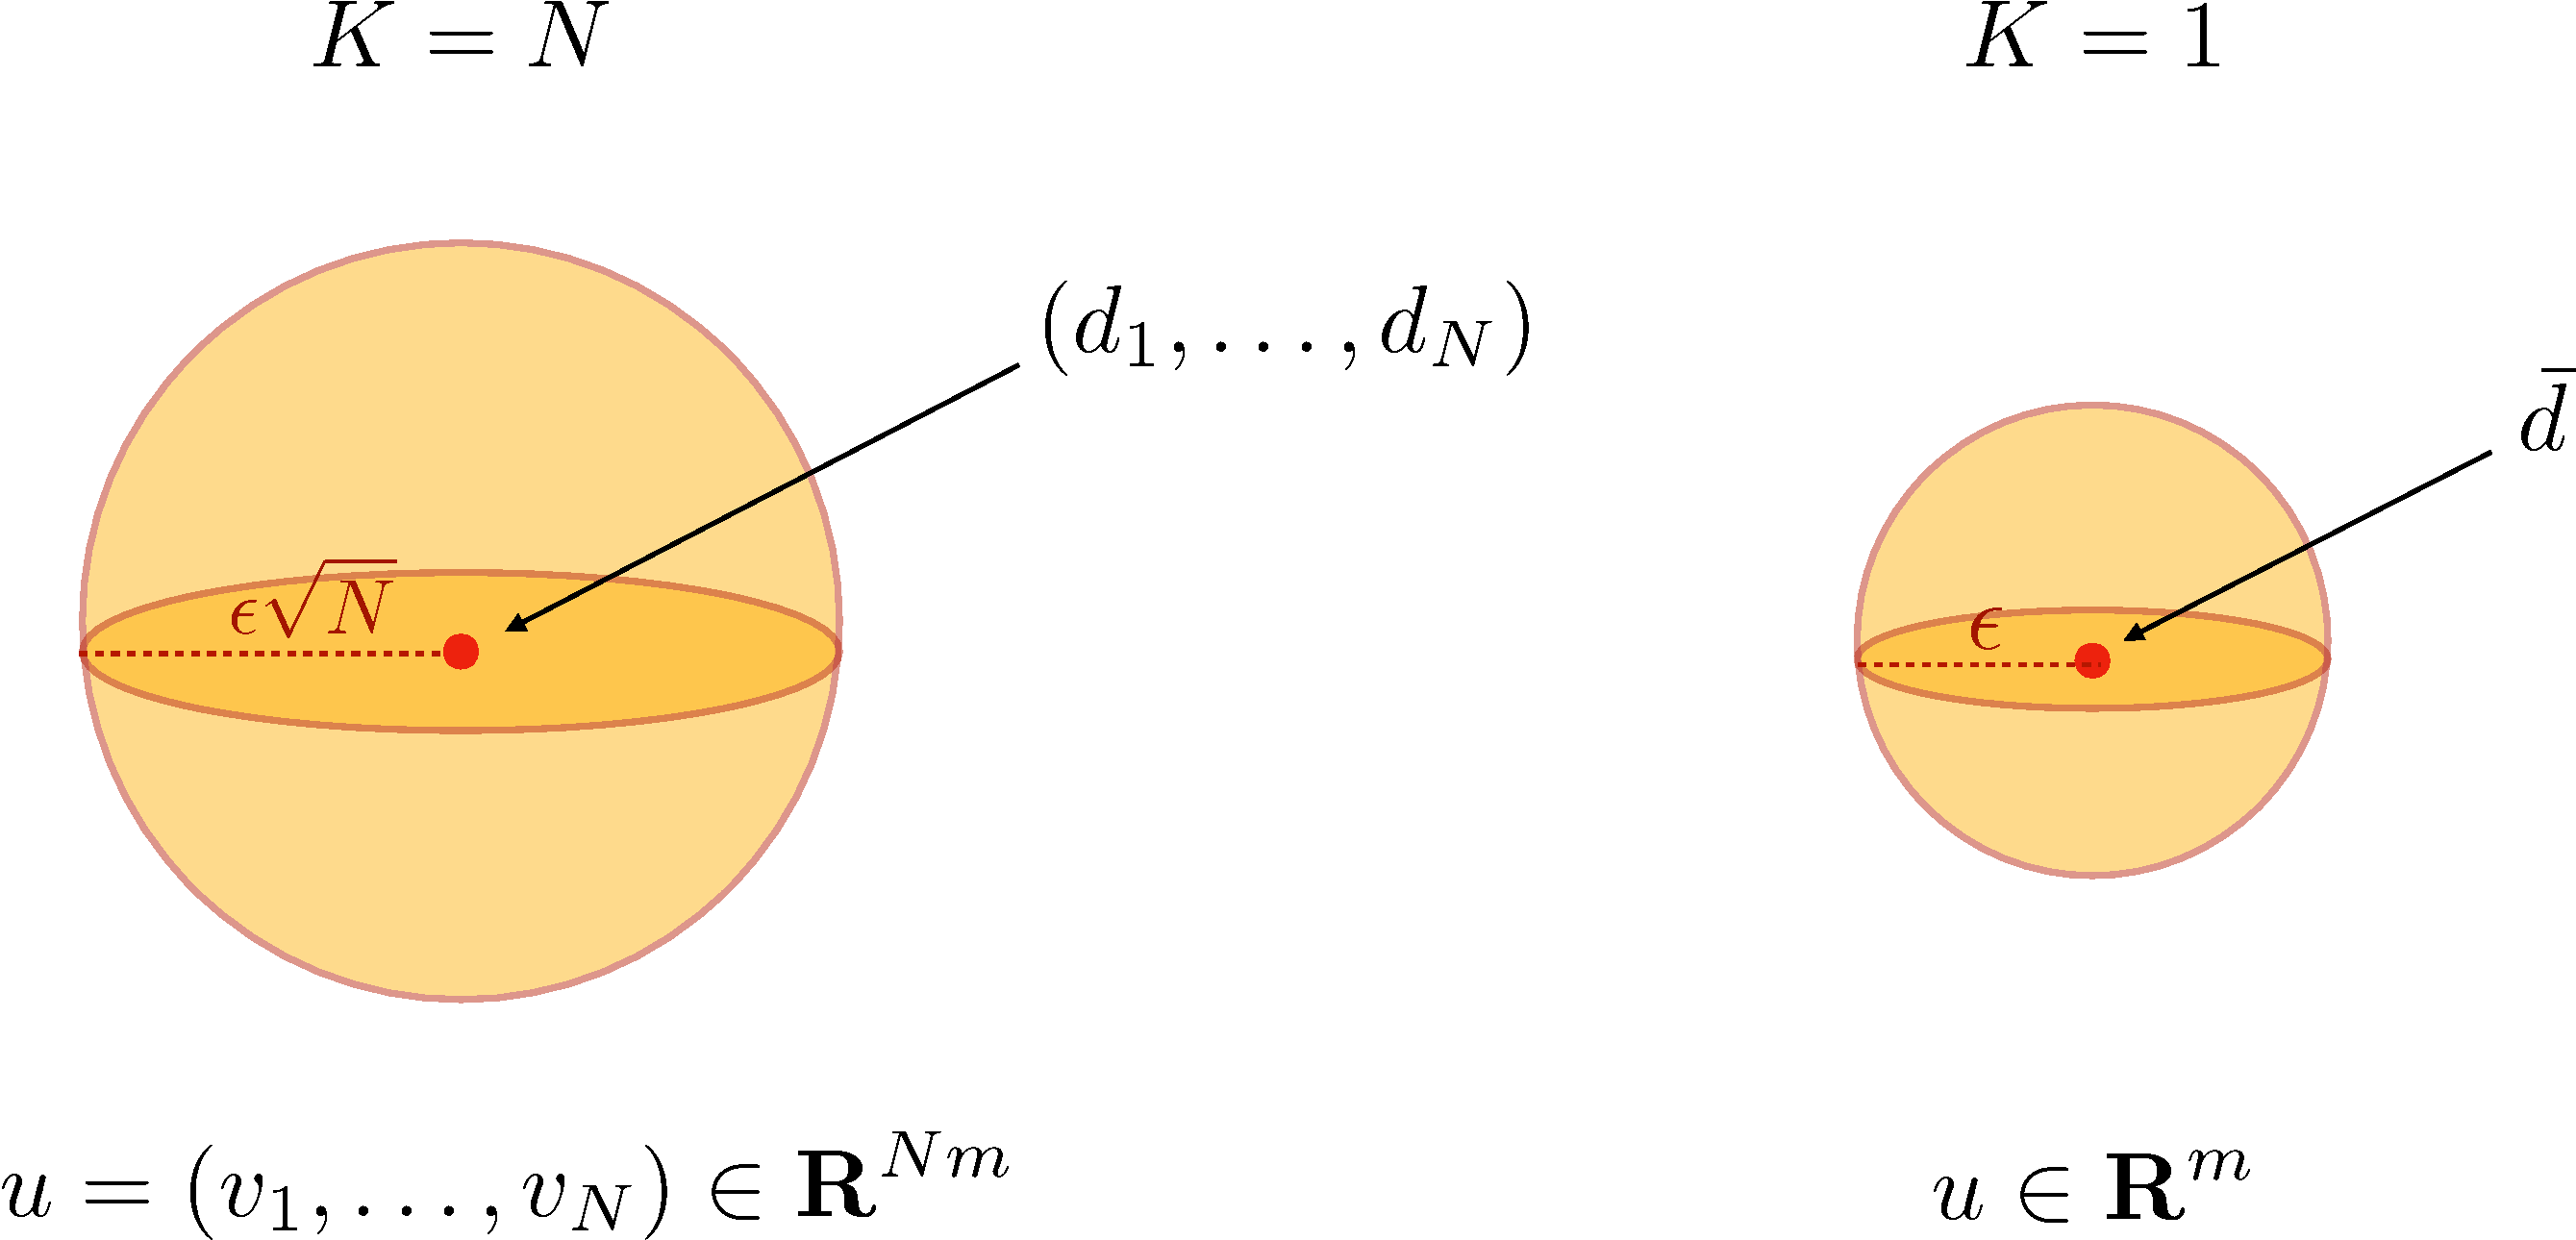
\includegraphics[width=0.6\textwidth]{unset_crop.pdf}
	\caption{Visualizing the uncertainty set $\uncset(N, \epsilon)$ and $\uncset(1,\epsilon)$ as high dimension balls when $p = 2$.}%
	\label{fig:unset}%
\end{figure}

\paragraph{Case $p = \infty$.}
In the case where $p = \infty$, the set we consider takes a more specific form,
\begin{equation*}
	\label{eq:uncset_inf}
	\uncset(K, \epsilon) \define \left\{ u = (v_1,\dots,v_K) \in \supp^{K} \quad\middle|\quad \max_{k=1,\dots,K} \| v_k - \bar{d}_k \| \le \epsilon\right\},
\end{equation*}
where the constraints for individual $v_k$ become decoupled.
See Figure~\ref{fig:unset-p} for an example when $K = 3$ and $K = 1$.
This decoupling follows the result for the Wasserstein type $p = \infty$ metric \citep[Equation 2]{wass-p}, as our uncertainty set is analogous to the set of all distributions within Wasserstein-$\infty$ distance of $\bar{d}$.
We note that, if any of the decoupled constraints are violated, then $\lim_{p \rightarrow \infty} \sum_{k=1} ^K w_k \| v_k - \bar{d}_k \|^p \geq \epsilon^p$, and the summation constraint will be violated.
\begin{figure}[h]%
	\centering
	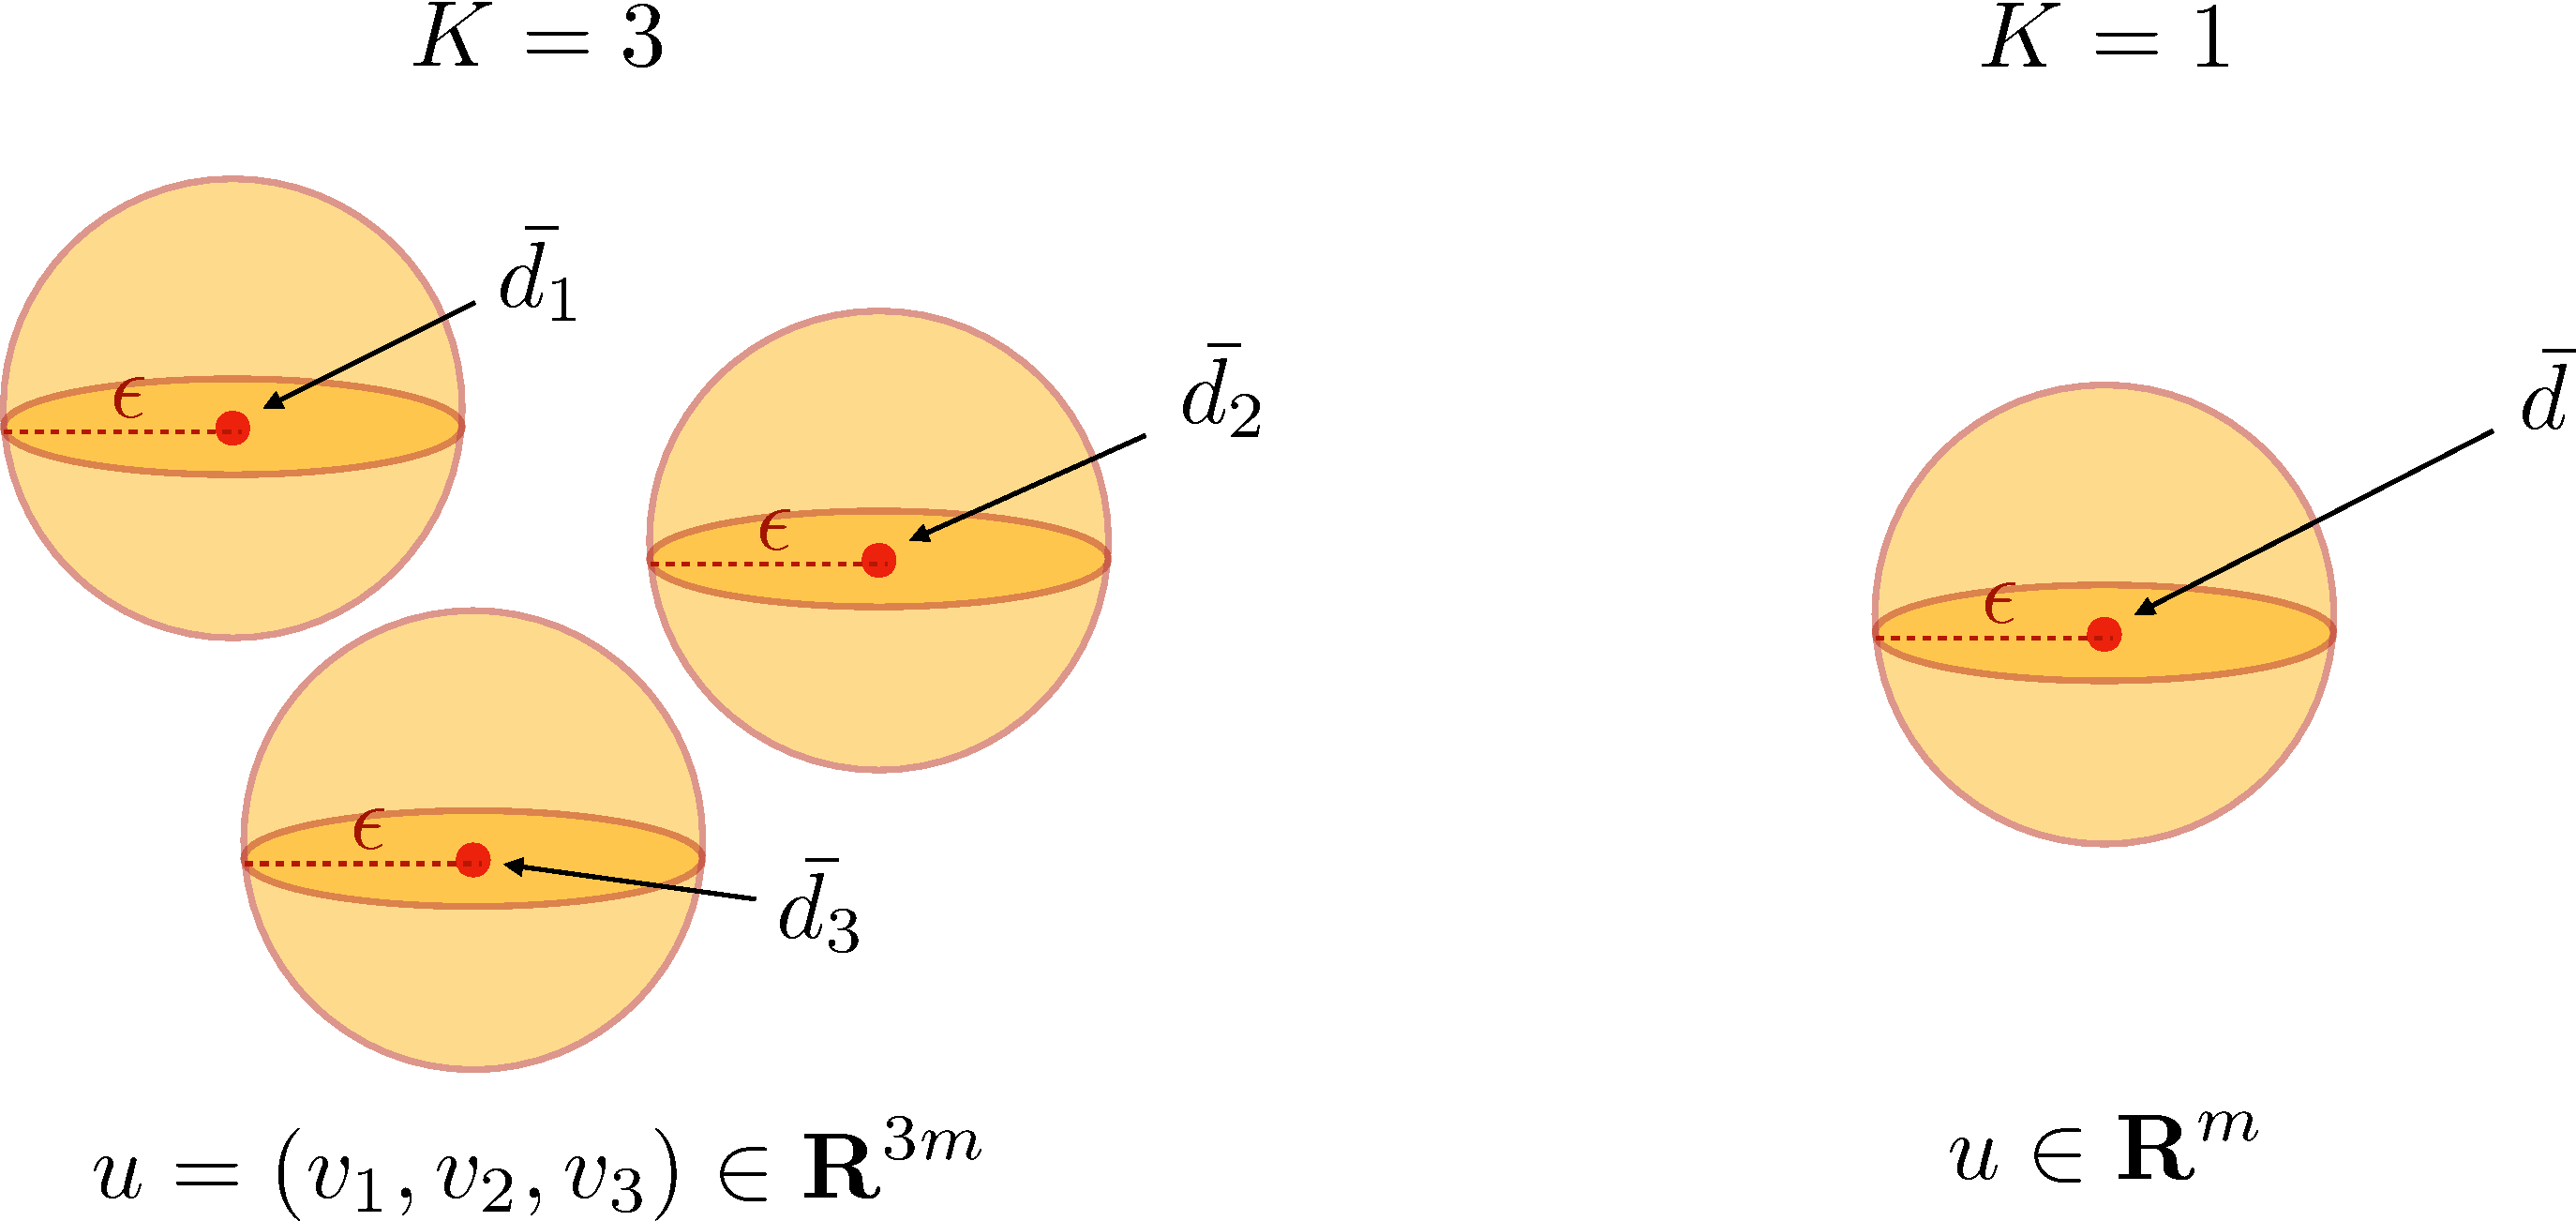
\includegraphics[width=0.6\textwidth]{unset_p_crop.pdf}
	\caption{Visualizing the decoupled uncertainty set $\uncset(K, \epsilon)$ with $p = \infty$.}%
	\label{fig:unset-p}%
\end{figure}

For both $p \geq 1$ and $p = \infty$, when~$K = 1$ we have a simple uncertainty set: a ball of radius $\epsilon$ around the empirical mean of the entire dataset, $\uncset(1, \epsilon) \define \left\{ v \in \supp \mid \| v - \bar{d} \| \le \epsilon  \right\}.$
This is equivalent to the uncertainty set of traditional \gls{RO}, as it is of the same dimension $m$ as the uncertain parameter.
When $K=N$ and $w_k = 1/N$, both cases closely resemble the ambiguity sets of Wasserstein-$p$ \gls{DRO}.
This formulation is thus a generalization of traditional sets for both~\gls{RO} and~\gls{DRO}.

Having defined the uncertainty set, we now introduce constraints of the form
\begin{equation}
	\label{eq:constraints}
\bar{g}(u, z) \define  \sum_{k=1} ^K w_k g(v_k, z),
\end{equation}
where $g$ is defined in the original constraint~\eqref{eq:constr_original}.
The weights $w_k$ correspond to the ones defined in the uncertainty set.
Putting everything together, $\hat{z}_N$ is the solution to the robust optimization problem
\begin{equation}
	\label{eq:robustopt}
	\tag{MRO}
	\begin{array}{ll}
		\mbox{minimize} & f(z)\\
		\mbox{subject to} & \bar{g}(u, z)  \le 0  \quad \forall u \in \uncset(K, \epsilon).
	\end{array}
	\end{equation}
	 We call this problem the \glsentryfull{MRO} problem.

\paragraph{High-level data-driven procedure.}%
\label{par:data_driven_procedure_}
Overall, given the problem data, we formulate the uncertainty set from clustered data using machine learning, with the choice of $K$ and $\epsilon$ chosen experimentally.
Then, we solve the \gls{MRO} problem to arrive at a data-driven solution $\hat{z}_N$ which satisfies the probabilistic guarantee~\eqref{eq:prob_guarantees1}, see Figure~\ref{fig:mro_proc}.
	\begin{figure}[h]%
		\centering
		\subfloat{{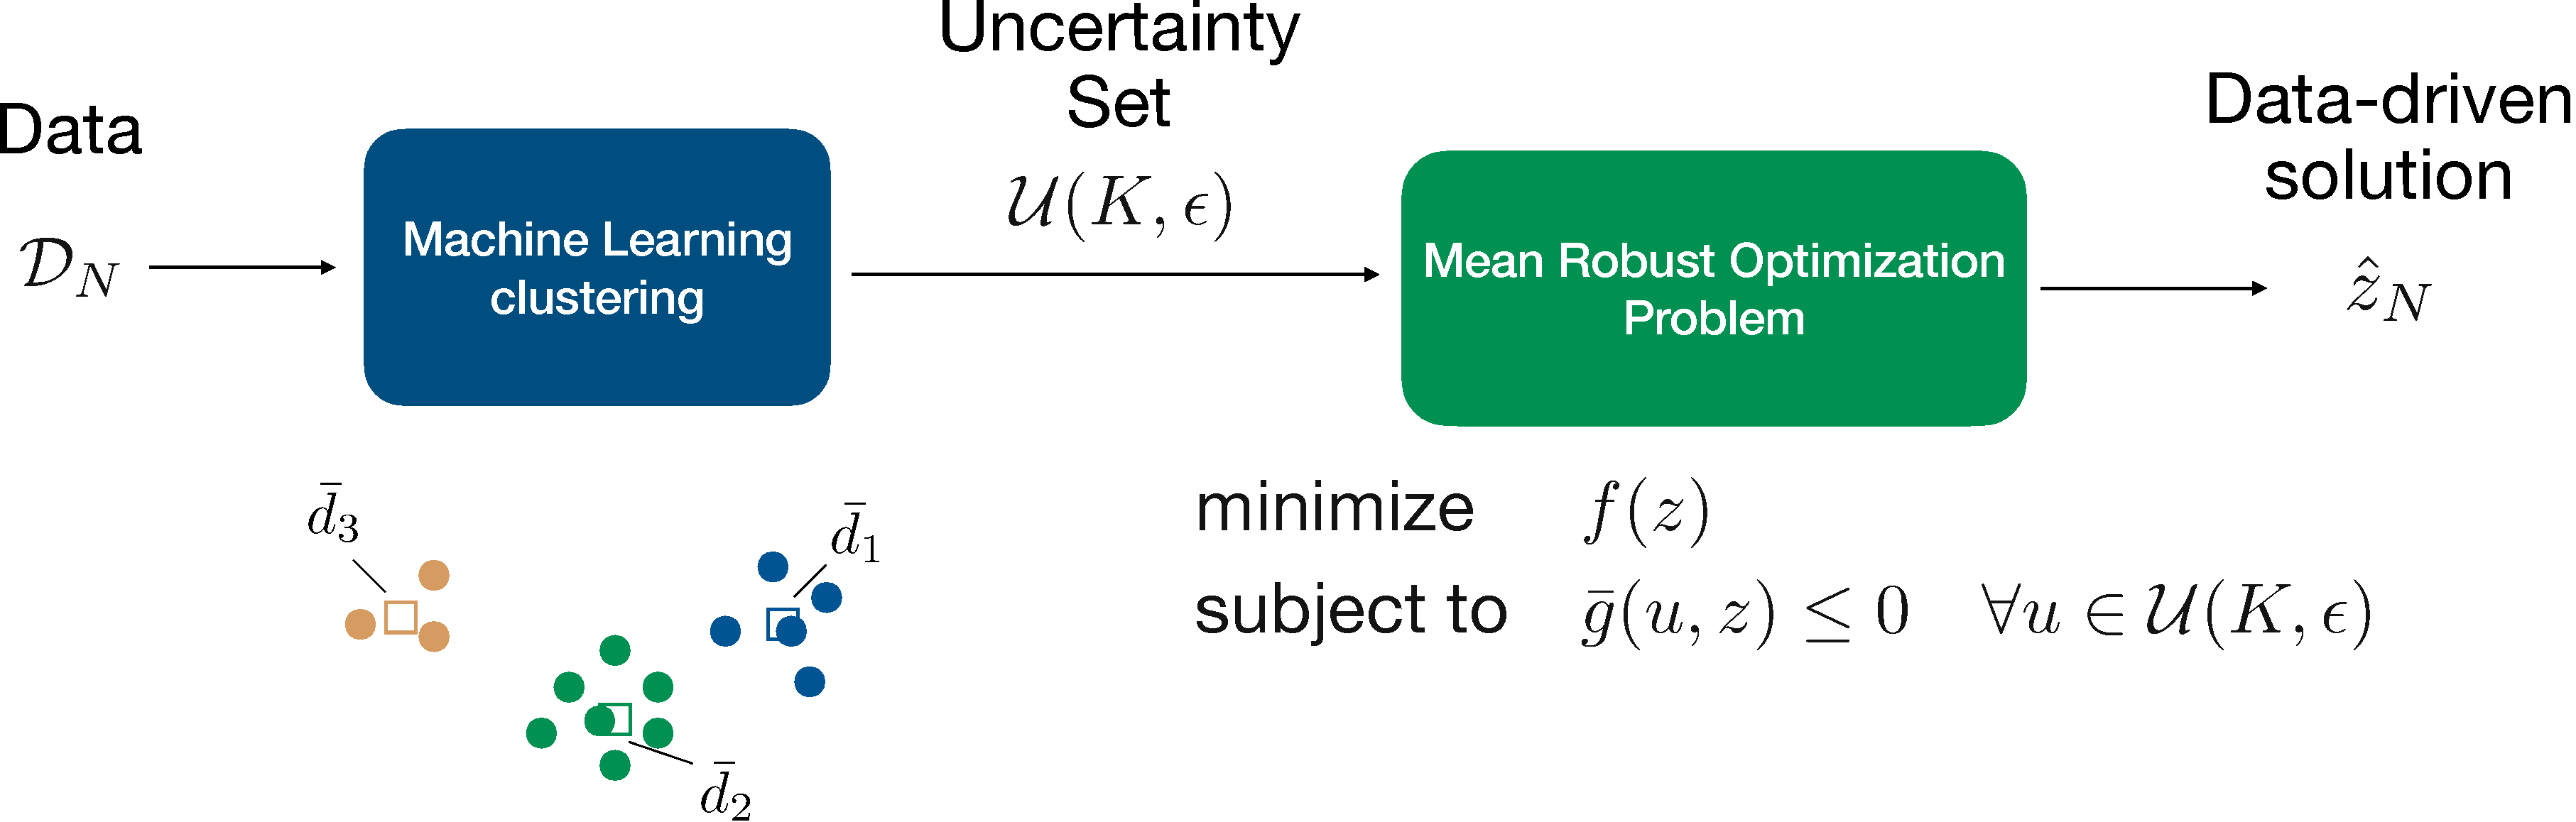
\includegraphics[width=0.9\linewidth]{procedure_crop.pdf} }}%
		\caption{Mean robust optimization procedure.}%
		\label{fig:mro_proc}%
	\end{figure}

\subsection{Solving the robust problem}
We now outline two ways to solve the~\gls{MRO} problem, using a direct convex reformulation and using a cutting plane algorithm. The reformulation and cutting plane procedure follow usual techniques for \gls{RO} problems in existing literature~\citep{ben-tal_robust_2009,kuhn2019wasserstein,robustadaptopt,cuttingplane}, with adaptations made for the \gls{MRO} setup, as well as a reformulation derived for the case $p = \infty$. We include simple examples and pseudocode for completeness.

\subsubsection{Direct convex reformulation for $p \geq 1$}
\label{sub:direct}
In the case where $p \geq 1$, the~\gls{MRO} problem can be rewritten as the optimization problem
\begin{equation}
	\label{eq:unif-const}
	% \tag{P}
	\begin{array}{ll}
		\mbox{minimize} & f(z)\\
		\mbox{subject to} & \begin{dcases}
			\begin{rcases}
		\underset{v_1, \dots, v_K \in \supp}{\text{maximize}} &\quad \sum_{k=1} ^K w_k g(v_k, z) \\
		\mbox{subject to} & \quad \sum_{k=1} ^K w_k \| v_k - \bar{d}_k \|^p \le \epsilon^p
			\end{rcases}
			\end{dcases} \le 0,
	\end{array}
\end{equation}
which, by dualizing the inner maximization problem, has the following reformulation for any $\epsilon > 0$:
\begin{equation}
	\label{eq:robustopt_p}
	\begin{array}{ll}
		\mbox{minimize} & f(z)\\
		\mbox{subject to} & \sum_{k=1}^{K} w_k s_k  \le 0\\
		& [-g]^*(y_{k} - h_{k}, z) + \sigma_{{\supp}}(h_{k}) - y_{k}^T\bar{d}_k  + \phi(q)\lambda \left\|y_{k}/\lambda \right\|^q_*  +\lambda \epsilon^p \leq s_k\\
		&\hspace{6cm} \quad k = 1,\dots, K\\
		& \lambda \geq 0,
	\end{array}
\end{equation}
with variables $\lambda \in \reals$, $s_k \in \reals$, $y_{k} \in \reals^{m}$, and $h_{k} \in \reals^m$.
Here, $[-g]^*(y, z) \define \sup_{u\in \dom g} y^Tu - [-g(u, z)] $ is the conjugate of $-g$, $\sigma_ \supp(y) \define\sup_{u \in  \supp}  y^Tu$ is the support function of $ \supp \subseteq \mathbf{R}^m$, $\| \cdot \|_*$ is the dual norm of  $\| \cdot \|$, and $\phi(q) = (q-1)^{(q-1)}/q^q$ for $q > 1$~\citep[Theorem 8]{kuhn2019wasserstein}.
Note that $q$ satisfies $1/p + 1/q = 1$, \ie, $q = p/(p - 1)$.
% is the conjugate number of $p \in [1,\infty)$.
\reviewChanges{When $p=1$ and $q =\infty$, we note the formulation in~\eqref{eq:robustp1}.}
The support function $\sigma_ \supp$ is also the conjugate of $\chi_ \supp$, which is defined $\chi_{\supp}(u) = 0$ if $u \in  \supp$, and $\infty$ otherwise.
The proof of the derivation and strong duality of the constraint is delayed to Appendix~\ref{app:dual_form}.
Since the dual of the constraint becomes a minimization problem, any feasible solution that with objective less than or equal to $0$ will satisfy the constraint, so we can remove the minimization to arrive at the above form.
While traditionally we take the supremum instead of maximizing, here the supremum is always achieved as we assume $g$ to be upper-semicontinuous.
For specific examples of the conjugate forms of different $g$, see Bertsimas and den Hertog~\cite[Section 2.5]{robustadaptopt} and Beck~\cite[Chapter 4]{amirbeck}.

When $K$ is set to be $N$, $w_k$ is $1/N$, and this is of an analogous form to the convex reduction of the worst case problem for Wasserstein \gls{DRO}; we expand upon this in Section~\ref{sub:connectionsdro}.

\reviewChanges{
We note the special case when $p = 1$. We observe from~\citep[Section 2.2 Remark 1]{kuhn2019wasserstein} that
\begin{equation*}
	 \lim_{q \rightarrow \infty}\phi(q)\lambda \left\|y_{k}/\lambda \right\|^q_* =
	\begin{dcases} 0 & \text{if}\; \|y_{k} \| \leq \lambda \\
		\infty & \text{otherwise}.
	\end{dcases}
	\end{equation*}
Therefore, the above formulation becomes
\begin{equation}
	\label{eq:robustp1}
	\begin{array}{ll}
		\mbox{minimize} & f(z)\\
		\mbox{subject to} & \sum_{k=1}^{K} w_k s_k  \le 0\\
		& [-g]^*(y_{k} - h_{k}, z) + \sigma_{{\supp}}(h_{k}) - y_{k}^T\bar{d}_k  + \lambda\epsilon^p\leq s_k\\
		&\hspace{6cm} \quad k = 1,\dots, K\\
		& \|y_{k} \| \leq \lambda, \quad k = 1,\dots, K\\
		& \lambda \geq 0.
	\end{array}
\end{equation}}


\paragraph{Example with affine constraints.}
Consider a single affine constraint of the form
\begin{equation}
	\label{eq:affineg}
	(a + Pu)^Tz \le b,
\end{equation}
where $a \in \reals^n$, $P \in \reals^{n \times m}$, and $b \in \reals$.
In other words, $g(u, z) = (a + Pu)^Tz - b$, and the support set is $\supp = \reals^m$.
Note that, in this case, $h_k$ must be $0$ for the support function $\sigma_{\supp}(h_k)$ to be finite.
%In addition, $q = p/(p-1) = 1$ and $\phi(q) = 1$.
We compute the conjugate as
\begin{equation}
\label{eq:conj_affine}
[-g]^*(y, z) =  \sup_u y^Tu +b - (a + Pu)^Tz =
\begin{dcases} a^Tz - b & \text{if}\; y + P^Tz = 0\\
	\infty & \text{otherwise}.
\end{dcases}
\end{equation}
To substitute $\sigma_{\supp}(h_k)$ and $[-g]^*(y_k - h_k, z)$ into~\eqref{eq:robustopt_p}, we note that $h_k = 0$ and $y_k = -P^Tz$, \ie, $y_k$ is independent from $k$.
Bycombining the $K$ constraints in~\eqref{eq:robustopt_p}, we arrive at the form
\begin{equation}
	\label{eq:example-affine-p}
	\begin{array}{ll}
		\mbox{minimize} & f(z)\\
		\mbox{subject to} & a^Tz - b + \phi(q)\lambda \left\|P^Tz/\lambda \right\|^q_*  +\lambda \epsilon^p + (P^Tz)^T\sum_{k=1}^{K} w_k \bar{d}_k \le 0\\
		& \lambda \ge 0,\\
	\end{array}
\end{equation}
where the number of variables or constraints does not depend on $K$.
Since vector $\sum_{k=1}^{K} w_k \bar{d}_k$ is the average of the datapoints in $\mathcal{D}_N$ for any $K \in \{1,\dots,N\}$, this formulation corresponds to always choosing $K=1$.


\subsubsection{Direct convex reformulation for $p = \infty$ }
\label{sub:direct-p}
In the case where ${p = \infty}$, the~\gls{MRO} problem can be rewritten as the optimization problem
\begin{equation}
	\label{eq:unif-const-p}
	% \tag{P}
	\begin{array}{ll}
		\mbox{minimize} & f(z)\\
		\mbox{subject to} & \begin{dcases}
			\begin{rcases}
		\underset{v_1, \dots, v_K \in\supp}{\text{maximize}} &\quad \sum_{k=1} ^K w_k g(v_k, z) \\
		\mbox{subject to} & \quad  \| v_k - \bar{d}_k \| \le \epsilon, \quad k = 1,\dots, K
			\end{rcases}
			\end{dcases} \le 0,
	\end{array}
\end{equation}
which has the following reformulation where the constraint above is dualized, for all $\epsilon > 0$:
	\begin{equation}
	\label{eq:unif-dual-p}
	% \tag{D}
	\begin{array}{ll}
		\text{minimize} & f(z)\\
 \text{subject to} \quad & \sum_{k=1}^{K} w_k s_k \leq 0\\
&[-g]^*(y_{k} - h_{k},z) + \sigma_{{\supp}}(h_{k}) - y_{k}^T\bar{d}_k  + \lambda_k \epsilon \leq s_k\\
& \hspace{3cm} \quad k = 1,\dots, K\\
&  \left\|y_{k} \right\|_* \leq \lambda_k \quad k = 1,\dots, K,
\end{array}
\end{equation}
with new variables $s_k \in \reals$, $y_{k} \in \reals^m$, and $h_{k} \in \reals^m$. The proof is delayed to Appendix~\ref{app:dual_form-p}.

\begin{remark}[Case ${p = \infty}$ is the limit of case ${p \geq 1}$]
	\label{limit-proof}
	In terms of the primal problem,~\eqref{eq:unif-const-p} is the limiting case of~\eqref{eq:unif-const} as $p \rightarrow \infty$.
	In terms of the reformulated problem with dualized constraints, problem~\eqref{eq:unif-dual-p} is the limiting case of~\eqref{eq:robustopt_p} as $p \rightarrow \infty$ .
	The proofs are delayed to Appendix~\ref{app:primal_limit} and Appendix~\ref{app:dual_limit} respectively. These proofs extend the ideas stated in~\cite[Proposition 3]{wass-p-1}.
\end{remark}

\paragraph{Example with affine constraints.}%
\label{par:example}
Consider again the case of affine constraint as in~\eqref{eq:affineg} with support set $\supp = \reals^m$, now with $p=\infty$.
Following a similar derivation as~\eqref{eq:example-affine-p}, we substitute the conjugate function $[-g]^*$~\eqref{eq:conj_affine} in problem~\eqref{eq:unif-dual-p}, we can obtain
\begin{equation}
	\label{eq:example-affine-inf}
	\begin{array}{ll}
		\mbox{minimize} & f(z)\\
		\mbox{subject to} & a^Tz - b + \epsilon\left\|P^Tz \right\|_* + (P^Tz)^T\sum_{k=1}^{K} w_k \bar{d}_k \le 0,\\
	\end{array}
\end{equation}
where the number of constraints and variables does not depend on $K$.
Similarly to problem~\eqref{eq:example-affine-p}, the term $\sum_{k=1}^{K} w_k \bar{d}_k$ is the average of the datapoints in $\mathcal{D}_N$ for any $K \in \{1,\dots,N\}$. Therefore, the choice of $K$ does not affect this formulation.
\reviewChanges{This can be viewed as the robust counterpart when the uncertainty set is a norm ball of radius $\epsilon$ centered at $(1/N)\sum_{i=1}^N d_i$}

Note that, if $\bar{d} = 0$ the constraint can be simplified even further, obtaining ${a^Tz + \epsilon\|P^Tz\|_* \le b}$, which corresponds to the robust counterpart in \gls{RO} with norm uncertainty sets~\citep[Section 2.3]{robustadaptopt},~\citep[Chapter 2]{ben-tal_robust_2009}.

\begin{remark}
	When $g$ is affine and \reviewChanges{$\supp = \reals^m$}, for any $\epsilon$ and norm, the convex reformulations for $p = 1$ and $p = \infty$ are identical. The proof appears in Appendix~\ref{app:equivalence}.
\end{remark}


\subsubsection{Cutting plane algorithm}
The second approach to solve problem~\eqref{eq:robustopt} is to use a cutting plane procedure, in which we consider the minimization problem where $z$ is the variable and $S$ a finite set of values for the uncertainty,
\begin{equation}
	\label{eq:mro_min}
	\begin{array}{ll}
		\mbox{minimize} & f(z)\\
		\mbox{subject to} & \bar{g}(u, z)  \le 0, \quad \forall u \in
		\hat{S},
		\end{array}
\end{equation}
and the maximization problem over $u$ with $z^k$ fixed,
\begin{equation}
	\label{eq:mro_max}
	\begin{array}{ll}
		\mbox{maximize} & \bar{g}(u, z^k)\\
		\mbox{subject to} & u \in \uncset(K, \epsilon)
	\end{array}
\end{equation}
The procedure works as follows.
We first solve~\eqref{eq:mro_min} with a set $\hat{S} = \{\bar{u}\}$, where $\bar{u}$ is nominal value of the uncertainty, obtaining $z^k$.
Then, we solve~\eqref{eq:mro_max}, obtaining $u^k$.
If $\bar{g}(u^k, z^k) > 0$, then we add $u^k$ to the set $\hat{S}$.
Otherwise, we terminate. This procedure is summarized in Algorithm~\ref{alg:cutting_plane}.
As demonstrated by Bertimas et al.~\cite{cuttingplane}, the cutting plane and convex reformulation methods are comparable in terms of performance, thus both are viable.
\begin{algorithm}
	\caption{Cutting plane algorithm to solve~\eqref{eq:robustopt}}
	\label{alg:cutting_plane}
	\begin{algorithmic}[1]
	 \State {\bf given} $\hat{S} = \{\bar{u}\}$
	 \For{$k=1,\dots,k_{\rm max}$}
	 \State $z^k \gets $ solve minimization problem~\eqref{eq:mro_min} over $z$
	 \State $u^k \gets $ solve maximization problem~\eqref{eq:mro_max} over $u$
         \If{$\bar{g}(u^{k}, z^{k}) > 0$}
	 \State $\hat{S} \gets \hat{S} \cup \{u^k\}$
	 \Else
	 \State {\bf return} $z^k$
	 \EndIf
	 \EndFor
	\end{algorithmic}
\end{algorithm}

\subsection{\reviewChanges{Maximum-of-concave constraint function}}
\label{sec:max_concave}
\reviewChanges{We now consider the general maximum-of-concave function satisfying Assumption~\ref{ass:convex_l}: 
$$g(u, z) = \max_{j\leq J}g_j(u, z),$$ with each $-g_j$ being proper, convex, and lower-semicontinuous in~$u$ for all $z$. When we take $J=1$, we arrive back at the formulations given in Section~\ref{sec:mro}.
Note that any problem with multiple uncertain constraints ${g_j(u,z),\; j = 1,\hdots,J}$, where we assume the usual conditions on $g_j$, can be combined to create a joint constraint of this maximum-of-concave form. 
As mentioned in Section~\ref{sec:intro}, this can also be used to model $\CVaR$ constraints, which has a maximum-of-concave analytical form.}

With the maximum-of-concave $g$ , we construct the~\gls{MRO} constraint as
\begin{equation}
	\label{eq:constraints_max}
\bar{g}(u, z) \define  \sum_{k=1}^K\sum_{j=1}^J \alpha_{jk} g_j(v_{jk}, z),
\end{equation}
where $\alpha\in \Gamma $, with $\Gamma = \{\alpha~|~\sum_{j=1}^J\alpha_{jk}= w_k, \alpha_{jk}\geq 0 ~\forall k,j\}$. For each constituent function $g_j$, the uncertainty set contains a set of vectors $(v_{j1},\dots,v_{jK})$, and a set of parameters $(\alpha_{j1},\dots, \alpha_{jK})$ to denote the fraction of mass assigned to that function for each $k$. The total amount of mass assigned for each cluster, $\sum_{j=1}^J\alpha_{jk}$, is the weight of the cluster, $w_k$. 

\reviewChanges{We use a summation over weighted pieces $g_j$ instead of a maximum over $g_j$, as this is a generalization of the maximum, and has a more natural dual reformulation. We take inspiration from~\citep[Section 4.2]{mohajerin_esfahani_data-driven_2018}, where $\alpha$ arises from the extremal distribution for Wasserstein \gls{DRO}.
Note that the intuitive maximization over $g_j$'s is analogous to setting $\alpha_{jk} = w_k$ for a specific $j$ for each $k$, and $\alpha_{jk} = 0$ otherwise.}

\reviewChanges{The uncertainty set is given as follows.}
\reviewChanges{
\paragraph{Case $p \geq 1$.}
In the case where $p \geq 1$, we have
\begin{equation*}
	\label{eq:uncset_p_max}
	\uncset(K, \epsilon) \define \left\{ u = (v_{11},\dots,v_{JK}) \in \supp^{K\times J} \quad\middle|\quad \sum_{k=1}^K \sum_{j=1}^J \alpha_{jk} \| v_{jk} - \bar{d}_k \|^p \le \epsilon^p,\alpha \in \Gamma \right\}.
\end{equation*}
Note that the single concave case given previously follows when we take $J = 1$. All parameters are defined as in the single concave case.}

\reviewChanges{\paragraph{Case $p = \infty$.}
In the case where $p = \infty$, the set we consider becomes
\begin{equation*}
	\label{eq:uncset_inf_max}
	\uncset(K, \epsilon) \define \left\{ u = (v_{11},\dots,v_{JK}) \in \supp^{K\times J} \quad\middle|\quad \max_{k=1,\dots,K} \sum_{j=1}^J (\alpha_{jk}/w_k) \| v_{jk} - \bar{d}_k \| \le \epsilon, \alpha \in \Gamma\right\},
\end{equation*}
where we once again introduce weight parameters $\alpha$. 
}

\reviewChanges{
Following these changes, $\hat{z}_N$ is again the solution to the robust optimization problem~\eqref{eq:robustopt}, defined now with the generalized uncertainty set and constraint.
}
\paragraph{\reviewChanges{Solving the robust problem.}}
\reviewChanges{We give the direct reformulation approach for solving the generalized problem for $p \geq 1$. The case $p = \infty$ is delayed to Appendix~\ref{app:dual_form-p_max}}.
\reviewChanges{We write the~\gls{MRO} problem as the optimization problem
\begin{equation}
	\label{eq:unif-const_max}
	% \tag{P}
	\begin{array}{ll}
		\mbox{minimize} & f(z)\\
		\mbox{subject to} & \begin{dcases}
			\begin{rcases}
		\underset{v_{11},\dots,v_{JK} \in \supp, \alpha \in \Gamma}{\text{maximize}} &\quad \sum_{k=1} ^K \sum_{j=1}^J \alpha_{jk} g_j(v_{jk}, z) \\
		\mbox{~~~~subject to} & \quad \sum_{k=1}^K \sum_{j=1}^J \alpha_{jk} \| v_{jk} - \bar{d}_k \|^p \le \epsilon^p\\
			\end{rcases}
			\end{dcases} \le 0,
	\end{array}
\end{equation}
and, by dualizing the inner maximization problem, arrive at the reformulation for all $\epsilon > 0$:}
\reviewChanges{
\begin{equation}
	\label{eq:robustopt_p_max}
	\begin{array}{ll}
		\mbox{minimize} & f(z)\\
		\mbox{subject to} & \sum_{k=1}^{K} w_k s_k  \le 0\\
		& [-g_j]^*(y_{jk} - h_{jk}, z) + \sigma_{{\supp}}(h_{jk}) - y_{jk}^T\bar{d}_k  + \phi(q)\lambda \left\|y_{jk}/\lambda \right\|^q_*  +\lambda \epsilon^p \leq s_k\\
		&\hspace{4cm} \quad k = 1,\dots, K, \quad j =1, \dots, J\\
		& \lambda \geq 0,
	\end{array}
\end{equation}
with variables $\lambda \in \reals$, $s_k \in \reals$, $y_{jk} \in \reals^{m}$, and $h_{jk} \in \reals^m$. The proof is delayed to Appendix~\ref{app:dual_form_max}.
Again, while traditionally we take the supremum instead of maximizing, here the supremum is always achieved as we assume \reviewChanges{$g_j$ to be upper-semicontinuous for all $j$.}}

\reviewChanges{In addition, when $K$ is set to be $N$, and $w_k$'s are $1/N$, this is also of an analogous form to the convex reduction of the worst case problem for Wasserstein \gls{DRO}, described below.


\section{Links to Wasserstein \gls{DRO}}
\label{sub:connectionsdro}
% \Glsentryfull{DRO} solves the problem
% where the ambiguity set $\mathcal{P}_N$ contains, with high confidence, all distributions that could have generated the training samples $\mathcal{D}^N$, such that the probabilistic guarantee~\eqref{eq:prob_guarantees1} is satisfied.
% Wasserstein \gls{DRO} constructs $\mathcal{P}_N$ as a ball of radius $\epsilon$ with respect to the Wasserstein metric around the empirical distribution ${\hat{\prob}^N \define \sum_{i=1}^N \delta_{d_i}/N}$, where $\delta_{d_i}$ denotes the Dirac distribution concentrating unit mass at $d_i \in \mathbf{R}^m$.
% Specifically, we write
% \begin{equation*}
% 	\label{eq:Wball}
% 	\mathcal{P}_N = \mathbf{B}_\epsilon^p (\hat{\prob}^N) \define \{\mathbf{Q} \in \mathcal{M}(\supp) \mid W_p(\hat{\prob}^N,\mathbf{Q}) \leq \epsilon \},
% \end{equation*}
% where $\mathcal{M}(\supp)$ is the set of probability distributions supported on $\supp$ satisfying a light-tailed assumption (more details in section~\ref{par:gau}), and
% $$W_p(\mathbf{Q},\mathbf{Q'}) \define \inf \left\{ \left(\int_\reviewChanges{\supp} \|u - u'\|^p \Pi (\dif u,\dif u') \right)^{1/p} \right\}.$$
% % This appears already in the next section
% % The probability distributions are assumed to satisfy ${\Expect^\mathbf{Q}(\|u\|^p)= \int_{\supp} \|u\|^p \mathbf{Q}(\dif u) < \infty}$ on convex and closed support $\supp$, $p > 1$ is any integer greater than 1, and $\Pi$ is any joint distribution of $u$ and $u'$ with marginals $\mathbf{Q}$ and $\mathbf{Q'}$.
% % The probability distributions are assumed to satisfy ${\Expect^\mathbf{Q}(\|u\|^p)= \int_{\supp} \|u\|^p \mathbf{Q}(\dif u) < \infty}$ on convex and closed support $\supp$,
% Here, $p$ is any integer greater than 1, and $\Pi$ is any joint distribution of $u$ and $u'$ with marginals $\mathbf{Q}$ and $\mathbf{Q'}$.


When $K=N$, the constraint of~\eqref{eq:robustopt} is equivalent to the constraint of the Wasserstein~\gls{DRO} problem
\begin{equation}
	\label{eq:dro_prob}
	\begin{array}{ll}
		\mbox{minimize} & f(z)\\
		\mbox{subject to} &   \sup_{\mathbf{Q}\in \mathcal{P}_N} \Expect_\mathbf{Q}(g(u,z))  \le 0,
	\end{array}
	\end{equation}
where the ambiguity set is as introduced in Chapter~\ref{chap:prelim}.
In particular, for the case $p \geq 1$, the Wasserstein~\gls{DRO} risk
\begin{equation}
\label{eq:dro-reduct}
\begin{aligned}
    \sup_{\mathbf{Q}\in \mathbf{B}_\epsilon^p(\hat{\prob}^N)} \Expect_\mathbf{Q}(g(u,z))
	\end{aligned}
\end{equation}
is equivalent to the dual of the constraint of~\eqref{eq:unif-const_max}, when $K = N$, and $w_k = 1/N$. 
This is noted in~\citep{kuhn2019wasserstein,zhen2021mathematical}.
We give a proof of strong duality in Appendix~\ref{app:convex_red}.
This is the dual of the generalized max-of-concave form, which is equivalent to the dual of the single concave form~\eqref{eq:unif-const} when $J = 1$. 
Bythe same logic, in the case where $p = \infty$, the expression is equivalent to the dual of the constraint of~\eqref{eq:unif-const-p}.
Given the above reductions, we can rewrite the Wasserstein \gls{DRO} problem in the same form as~\eqref{eq:unif-const_max}, the \gls{MRO} problem.

Our approach can then be viewed as a form of Wasserstein \gls{DRO}, with the difference that, when $K<N$, we deal with the clustered and averaged dataset.
We construct $\mathcal{P}_N$ as a ball around the empirical distribution $\hat{\prob}^K$ of the centroids of our clustered data
\begin{equation*}
\hat{\prob}^K \define \sum_{k=1}^K w_k\delta_{\bar{d}_k},
\end{equation*}
where $w_k$ is the proportion of data in cluster $k$.
This formulation allows for the reduction of the sample size while preserving key properties of the sample, which translates directly to a reduction in the number of constraints and variables.

\subsection{Satisfying the probabilistic guarantees}
\label{par:gau}
As we have noted the parallels between \gls{MRO} and Wasserstein \gls{DRO}, we now show that the conditions for satisfying the probabilistic guarantees are also analogous. Byenlarging the Wasserstein ball by a clustering-dependent value $\eta_N(K)$, we ensure that the measure-concentration type results from Section~\ref{sec:gua_dependent} hold also for~\gls{MRO}.
% \paragraph{Case $p \geq 1$.} Wasserstain \gls{DRO} satisfies~\eqref{eq:prob_guarantees1} if the data-generating distribution, supported on a convex and closed set $\supp$, satisfies a {\it light-tailed assumption}~\citep{fournier_guillin_2013,mohajerin_esfahani_data-driven_2018}: there exists an exponent $a > 0$ and $t > 0 $ such that ${A = \Expect^{\prob}(\exp (t \|u \|^a))  = \int_{\reviewChanges{\supp}} \exp (t \| u \| ^a) \prob(du) < \infty.}$
% We refer to the following theorem.
% \begin{theorem}[Measure concentration {\citep[Theorem 2]{fournier_guillin_2013}}]
% \label{theorem_ball}
% If the light-tailed assumption holds, we have
% 	\begin{equation*}
% 	\prob^N(W_p(\prob,\hat{\prob}^N) \geq \epsilon) \le \phi(p, N, \epsilon),
% 	\end{equation*}
% where $\phi$ is an exponentially decaying function of $N$.
% \end{theorem}
% % \begin{theorem}[Measure concentration \citep{fournier_guillin_2013}]
% % \label{theorem_ball}
% % If the light-tailed assumption holds, when p = 1 and $a > 1$, we have
% % \begin{equation*}
% %         \prob^N(W_1(\prob,\hat{\prob}^N) \geq \epsilon)
% %         \leq \begin{cases}
% %                 c_1 \exp(-c_2N \epsilon^{\max\{m,2\}}) \quad \textit{if } \epsilon \leq 1\\
% %                 c_1 \exp(-c_2N \epsilon^{a}) \quad \textit{if }  \epsilon > 1,
% %         \end{cases}
% % \end{equation*}
% %         for all $\epsilon > 0$, $m \neq 2$, and $N \geq 1$. When $p \geq 2$, and $\alpha \in (0,p)$, we have
% %         $$	\prob^N(W_p(\prob,\hat{\prob}^N)^p \geq \epsilon^p)
% %         \leq \begin{cases}
% %                 c_1 \exp(-c_2N \epsilon^{\max\{m,2p\}}) + \exp(-c_2 (N\epsilon^p)^\frac{a-s}{p})  \quad \textit{if } \epsilon \leq 1, \forall s \in (0,a)\\
% %                 c_1 \exp(-c_2 (N \epsilon^p)^{a/p}) \quad \textit{if }  \epsilon > 1,
% %         \end{cases}$$
% %         for all  $\epsilon > 0$, $m \neq 4$, and $N \geq 1$. $c_1,c_2$ are positive constants depending only on $A,a,t, s,$ and $m$.
% % \end{theorem}
% Theorem~\eqref{theorem_ball} estimates the probability that the unknown data-generating distribution $\prob$ lies outside the Wasserstein ball $\mathbf{B}_\epsilon^p (\hat{\prob}^N)$, which is our ambiguity set.
% Thus, we can estimate the smallest radius $\epsilon$ such that the Wasserstein ball contains the true distribution with probability $1 - \beta$, for some target $\beta \in (0,1)$.
% We equate the right-hand-side to $\beta$, and solve for $\epsilon_N(\beta)$ that provides us the desired guarantees for Wasserstein \gls{DRO}~\citep[Theorem 3.5]{mohajerin_esfahani_data-driven_2018}.


% \paragraph{Case $p = \infty$.} When $p = \infty$, Bertsimas et al.~\cite[Section 6]{wass-p-1} note that the light-tailed assumption is no longer sufficient.
% Wasserstein \gls {DRO} satisfies~\eqref{eq:prob_guarantees1} under stronger assumptions, as given in the following theorem.
% \begin{theorem}[Measure concentration, $\mathbf{p = \infty}$ {\cite[Theorem 1.1]{wass-p-guarantee}}]
% \label{theorem-inf}
% 	Let the support $\supp \subset \reals^m$ of the data-generating distribution be a bounded, connected, open set with Lipschitz boundary. Let $\prob$ be a probability measure on  $\supp$ with density $\rho : \supp \rightarrow(0,\infty)$, such that there exists $\lambda \geq 1$ for which ${1/\lambda \leq \rho(x) \leq \lambda, \hspace{2mm} \forall x \in \supp}$. Then,
% 	\begin{equation*}
% 		\prob^N(W_\infty(\prob,\hat{\prob}^N) \geq \epsilon) \le \phi(N, \epsilon),
% 		\end{equation*}
% 	where $\phi$ is an exponentially decaying function of $N$.
% \end{theorem}
% We can again equate the right-hand-side to $\beta$ and find  $\epsilon_N(\beta)$. We extend this result to the clustered set in \gls{MRO}.

\begin{theorem}[\gls{MRO} finite sample guarantee] \label{theorem_mro} Assume the light-tailed assumption~\ref{ass:light_tail} holds when $p \geq 1$, and the assumptions of Theorem~\ref{theorem-inf} hold when $p = \infty$. If ${\beta \in (0,1]}$, $\eta_N(K)$ is the average $p$-th powered distance of data-points in $\mathcal{D}_N$ from their assigned cluster centers, and $\hat{z}_N$ is the optimal solution to~\eqref{eq:robustopt} with uncertainty set $\uncset(K,\epsilon_N(\beta) + \eta_N(K)^{1/p})$, then the finite sample guarantee~\eqref{eq:prob_guarantees1} holds.
\end{theorem}

\begin{proof}
Compared with Wasserstein \gls{DRO}, \gls{MRO} has to account for the additional difference between the two empirical distributions $\hat{\prob}^N$ and $\hat{\prob}^K$.
We can write
\begin{equation*}
	\begin{array}{ll}
		&\displaystyle \hat{\prob}^N \define \sum_{i=1}^N \frac{1}{N}\delta_{d_i} = \sum_{k=1}^K \sum_{i \in C_k} \frac{|C_k|}{N}\frac{1}{|C_k|}   \delta_{d_i}, \\ % = \sum_{k=1}^K w_k \frac{1}{|C_k|}\sum_{i \in C_k}  \delta_{d_i},\\
		&\displaystyle \hat{\prob}^K = \sum_{k=1}^K w_k\delta_{\bar{d}_k} = \sum_{i=1}^K \frac{|C_k|}{N}\delta_{\bar{d}_k}. % = \sum_{i=1}^K w_k \delta_{\frac{\sum_{i \in C_k} d_i}{|C_k|}},
		\end{array}
	\end{equation*}
If we introduce a new parameter, $\eta_N(K)$, defined as
\begin{equation*}
	\eta_N(K) =  \frac{1}{N} \sum_{i = 1}^K \sum_{i \in C_k} \|d_i - \bar{d}_k\|^p
	\end{equation*}
	 the average $p$-powered distance with respect to the norm used in the Wasserstein metric, of all data-points in $\mathcal{D}_N$ from their assigned cluster centers $\bar{d}_k$, we notice that
\begin{equation*}
	\begin{aligned}
	W_p(\hat{\prob}^K,\hat{\prob}^N)^p &= \inf_\Pi \left\{ \int_\reviewChanges{\supp} \|u - u'\|^p \Pi (\dif u,\dif u') \right\} \quad \text{($\Pi$ any joint distribution of $\hat{\prob}^K$, $\hat{\prob}^N$  )}\\
&=\sum_{i = 1}^K \frac{|C_k|}{N}  \int_\reviewChanges{\supp} \|u - \bar{d}_k\|^p \reviewChanges{\hat{\prob}^N(u|u' =\bar{d}_k)}({\rm d}u)\\
&\leq \sum_{i = 1}^K \frac{|C_k|}{N}  \frac{1}{|C_k|} \sum_{i \in C_k} \|d_i - \bar{d}_k\|^p\\
&= \eta_N(K),
	\end{aligned}
	\end{equation*}
where we have replaced the integral with a finite sum, as the distributions are discrete. Therefore, by Theorems~\ref{thm:measure_gen},~\ref{theorem-inf} and the \reviewChanges{triangle inequality for the Wasserstein metric~\cite{wass_tri}},
\begin{equation*}
	\begin{aligned}
	W_p(\prob,\hat{\prob}^K) &\leq W_p(\prob,\hat{\prob}^N) + W_p(\hat{\prob}^K,\hat{\prob}^N)\\
	&\leq \epsilon_N(\beta) + \eta_N(K)^{1/p},
\end{aligned}
	\end{equation*}
with probability at least $1 - \beta$. We thus have
\begin{equation*}
		\prob(\prob \in \mathbf{B}_{\epsilon_N(\beta) + \eta_N(K)^{1/p}}^p (\hat{\prob}^K) )\geq 1 - \beta,
	\end{equation*}
which implies the uncertainty set $\uncset(K, \epsilon_N(\beta) + \eta_N(K)^{1/p})$ contains all possible realizations of uncertainty with probability $1-\beta$, so the finite sample guarantee~\eqref{eq:prob_guarantees1} holds.
\end{proof}

This result introduces a tradeoff between conservatism (affected by the radius) and computational efficiency (affected by the sample size), controlled by the value of $K$. When a large $K$ is chosen, the effect on the radius is small, but the computational savings may also be minimal. The choice of $K$ is thus paramount.

One might note that a blanket increase in the radius regardless of the optimization problem may introduce unnecessary conservatism. This brings us to the next section, where we bring the constraint functions $g$ into our considerations. 


\section{Worst-case value of the uncertain constraint}
\label{sec:conservatism}
In the previous section, we proposed a theoretical increase in $\epsilon$ to maintain the same finite sample guarantee before and after clustering. 
However, a question remains: what is the extent of the effects of clustering if we {\it don't} increase $\epsilon$?
In this section, we thus approach the analysis in a different manner: keeping $\epsilon$ constant, we quantify the change in the {\it worst-case value of the constraint function} that arises from clustering. 
In fact, for select cases, our results suggest there is no need to increase $\epsilon$ after clustering; under specific curvature conditions on the  constraint function $g$, we may obtain a more conservative, or even unchanged solution after clustering, in which case the original finite sample guarantee is retained. 

We begin with a remark on the clustering value attained. The \gls{MRO} approach is closely centered around the concept of clustering to reduce sample size while maintaining sample diversity.
We wish to cluster points that are close together, such that the objective is only minimally affected. With this goal, we would like to minimize the average distance of the points in each cluster to their data-center,
\begin{equation*}
	D(K)^\star =\text{minimize } D(K) =  \text{minimize } \frac{1}{N}\sum_{k=1}^K \sum_{d_i \in C_k} \| d_i - \bar{d}_k \|^2_2,
\end{equation*}
	where $\bar{d}_k$ is the mean of the points in cluster $C_k$.
	While the best performance is attained with $D(K)^\star$, in practice we work with the approximation $D(K)$, where $C_k$ is decided by {\it any} clustering algorithm. This value upper bounds $D(K)^\star$. A well-known algorithm is $K$-means~\citep{kmeans}, where we create $K$ clusters by iteratively solving a least-squares problem.
	From here on we use only $D(K)$, and note that for the case $p=2$, we have $D(K)=\eta_N(K)$ from Theorem~\ref{theorem_mro}.

In this section, we then show the effects of clustering on the worst-case value of the constraint function in~\eqref{eq:robustopt}.
We prove two sets of results, corresponding to $g$ given as a single concave function, and as a more general maximum-of-concave function, which includes the maximum-of-affine function. Later, in Chapter~\ref{chap:online_dro} of this thesis, we show how these results imply finite-sample and asymptotic performance guarantees. 


\subsection{\reviewChanges{Single concave function}}
\label{sub:single-con}
For the simplest case of a single concave function, we prove that when the support is large enough,
\begin{itemize}
	\item If $g$ is affine in $u$, \gls{MRO} does not increase the worst-case value, regardless of $K$.
	\item If $g$ is concave in $u$ and satisfies certain smoothness conditions, \gls{MRO} has a higher worst-case value than Wasserstein \gls{DRO} and the increase is inversely related to the number of clusters~$K$. In other words, the smaller the $K$, the higher the worst-case value.
	%\item If $g$ is convex as the finite maximum of at least two affine functions, MRO is less conservative than Wasserstein DRO, and the level of conservatism increases with the number of clusters $K$.
\end{itemize}

\paragraph{Quantifying the clustering effect.}%
\label{par:quantify_clustering_effect_}
To quantify the effect of clustering, we calculate the difference between the following formulations of the worst-case value of the constraint in~\eqref{eq:robustopt}
\begin{equation}
	\tag{MRO-N}
	\begin{aligned}
	\label{eq:nocluster_one}
	\bar{g}^N(z) = \underset{v_1\dots v_N}{\text{maximize}} &\quad\frac{1}{N} \sum_{i=1} ^N g(v_i, z) \\
	\mbox{subject to} & \quad \frac{1}{N} \sum_{i=1} ^N  \| v_i - d_i \|^p \le \epsilon^p\\
	& \quad v_i\in \supp \quad i = 1,\dots,N,
	\end{aligned}
\end{equation}
\begin{equation}
	\tag{MRO-K}
	\label{eq:cluster_one}
	\begin{aligned}
		\bar{g}^K(z) = \underset{u_1\dots u_K}{\text{maximize}} &\quad  \sum_{k=1} ^K  \frac{|C_k|}{N} g(u_k, z) \\
	\mbox{subject to} & \quad\sum_{k=1} ^K \frac{|C_k|}{N}  \| u_k - \bar{d}_k \|^p \le \epsilon^p\\
	& \quad u_k\in \supp \quad k = 1,\dots,K,
	\end{aligned}
\end{equation}
and
\begin{equation}
	\tag{MRO-N*}
	\label{eq:nocluster_inf}
	\begin{aligned}
		\bar{g}^{N*}(z) = \underset{v_1\dots v_N}{\text{maximize}} &\quad\frac{1}{N} \sum_{i=1} ^N g(v_i, z) \\
		\mbox{subject to} & \quad \frac{1}{N} \sum_{i=1} ^N  \| v_i - d_i \|^p \le \epsilon^p,
		\end{aligned}
\end{equation}
where~\eqref{eq:nocluster_one} is the formulation of the constraint without clustering, akin to traditional Wasserstein \gls{DRO},~\eqref{eq:nocluster_inf} is the same, except we drop the support constraint, and~\eqref{eq:cluster_one} is the formulation with $K$ clusters.
\reviewChanges{
From here on, when we mention that the support {\it affects the worst-case constraint value}, we refer to situations where at least one of the constraints $v_i \in \supp$ for $i = 1,\dots,N$ is binding.
Formally, the definition is $\bar{g}^N(z) \neq \bar{g}^{N*}(z)$ for any $z$ feasible for the \gls{DRO} problem. 
We note a sufficient but not necessary condition for the support to not affect the worst-case constraint value: the situation in which the support doesn't affect the uncertainty set, which is defined as 
$$\left \{u \in \reals^{N\times m}: (1/N)\sum_{i=1}^N  \| u_i - d_i \| \le \epsilon\right \} = \left \{ u \in \supp^{N\times m}: (1/N)\sum_{i=1}^N \| u_i - d_i \| \le \epsilon\right \}.$$
If the support satisfies this condition, then we can conclude that $\bar{g}^N(z) = \bar{g}^{N*}(z)$ for any $z$ feasible for the \gls{DRO} problem, and obtain improved bounds below. 
While the condition depends on the location of the datapoints, it is acceptable to have this dependency, as this is a condition we can check given data to potentially improve the following bounds, without having to solve the MRO problem.}

With these definitions, we can construct solutions for~\eqref{eq:nocluster_one},~\eqref{eq:cluster_one}, and~\eqref{eq:nocluster_inf} to prove the following relations.
\begin{theorem}
	\label{thm:1}
	\reviewChanges{
	With the same $z$ and $\epsilon$, and for any integer $p \geq 1$, we always have $$\bar{g}^{N}(z) \le \bar{g}^K(z).$$
Furthermore, suppose that Assumption~\ref{assp:dom} holds, and $g$ satisfies an $L$-smooth condition on its domain with respect to the $\ell_2$-norm and for a given $z \in \mathcal{Z}$, \ie,
	\begin{equation*}
		\left\|\nabla g(v,z) - \nabla g(u,z)\right\|_2 \leq L\| u - v\|_2, \forall u,v \in \dom g.
	\end{equation*}
Then, with the same $z$ and $\epsilon$, and for any integer $p \geq 1$, we always have
	\begin{equation*}
	  \bar{g}^K(z) \leq \bar{g}^{N*}(z) + (L/2) D(K).
	\end{equation*}}
\end{theorem}
The proof is delayed to Appendix~\ref{app:thm1}. The results also hold for $p = \infty$, as we have shown in Remark~\ref{limit-proof} that the case $p = \infty$ is the limit of the case $p \geq 1$, and these results hold under the limit.
%We can extend this result to the case of specific convex functions.
%\begin{corollary}
%	\label{cor:1}
%If $g$ is convex in $u$, specifically taking the form of the maximum of affine pieces $g = \max_j g_j$, and satisfies an $L$-smooth condition with an extra constant $M$ with respect to the $\ell_2$-norm, then we always have
%\begin{equation*}
%	\begin{array}{ll}
%(i) &\bar{g}^N(x) \geq \bar{g}^K(x)\\
% (ii) &\bar{g}^K(x) \geq \bar{g}^N(x) - (L/2) D(K) -  \frac{M}{N} D_1(K).
%	\end{array}
%\end{equation*}
%\end{corollary}
%To prove this, we simply apply the previous theorem to $-g$.

\reviewChanges{Let $\Delta$ be the maximum difference in constraint value resultant from relaxing the support constraint on the \gls{MRO} uncertainty sets, \ie, ${\Delta = \max_{z\in \mathcal{Z}}\left(\bar{g}^{N*}(z) - \bar{g}^{N}(z)\right)}$, subject to $z$ being feasible for problem~\eqref{eq:robustopt}. 
As we assume Assumption~\ref{assp:dom} to hold, combined with the smoothness of $g$, we note that when solving for $\bar{g}^{N*}(z)$, the chosen $v_i$ values without the support constraint will still remain in the domain $\dom$ of $g$. 
Refer to a similar argument in Appendix~\ref{app:thm1} (ii) for details. 
The function $\bar{g}^{N*}(z) - \bar{g}^{N}(z)$ is then continuous in $z$ and everywhere defined for $z \in \mathcal{Z}$, thus maximizing with respect to $\mathcal{Z}$, a compact set, the value $\Delta$ is finite. }
Then, we observe that $ \bar{g}^K(z)  - \bar{g}^N(z)\leq \Delta +(L/2) D(K)$ for all such $z$, so the smaller the $D(K)$, (\ie, higher-quality clustering procedure), the smaller the increase in the worst-case constraint value. \reviewChanges{In addition, the value $\Delta$ is independent of $K$, as we calculate it with only $\bar{g}^{N*}(z)$ and $\bar{g}^{N}(z)$.}

\begin{remark} \label{rem:support}
	% Since we are solving a \gls{DRO} problem, we only consider uncertainty within $\epsilon-$balls of our datapoints, which can be interpreted as manually constructing a new support for the uncertain data.
% When $\epsilon$ is small and we have high confidence the support will not constrain the uncertainty set, we can remove the support constraint by setting $\supp = \dom{g}$ and arrive at $\Delta = 0$.
While $\Delta$ could be constructed to be arbitrarily bad, in practice, we expect our relevant range of $\epsilon$ to be small enough such that the difference is insignificant.
We can then approximate $\Delta \approx 0$ and simply use the upper bound $(L/2)D(K)$, as this bound is often not tight.
See Sections~\ref{sub:facility} and~\ref{sub:capitalbudget} for examples. Later in Section~\ref{lem:delta}, we give more specific bounds for $\Delta$. 
\end{remark}

\paragraph{Uncertain objective.}%
\label{par:uncertain_objective_}
When the uncertainty is in the objective, Theorem~\ref{thm:1} quantifies the difference in optimal values.
% such that an uncertain constraint can be created using the epigraph form of the objective function, we note the following corollary.
\begin{corollary}
	\label{cor:obj_unc}
Consider the problem where $g$ is itself the objective function we would like to minimize and $X \subseteq \reals^n$ represents the constraints, which are deterministic.
Then, $(L/2)D(K)$ + $\Delta$ upper bounds the difference in optimal values of the \gls{MRO} problem with $K$ and $N$ clusters.
\end{corollary}

% \begin{proof}
% The feasible region of the \gls{MRO} problem with $K$ and $N$ does not change with clustering, as there are no constraints that involve the uncertain parameter.
% From Theorem~\ref{thm:1}, for any fixed $\hat{x}$,  we have $\bar{g}^K(\hat{x}) - \bar{g}^N(\hat{x}) \leq  (L/2) D(K) + \Delta$.
% Therefore, no matter what $\hat{x}$ the \gls{MRO} problem with $K$ clusters selects, the \gls{MRO} problem with $N$ clusters can always choose the same $\hat{x}$ to be at most $(L/2) D(K) + \Delta$ lower in value.
% \end{proof}

% The difference in the level of conservatism of the two problems then directly depend on $D(K)$.

\paragraph{Uncertain constraints.}%
\label{par:uncertain_constraints_}
When the uncertainty is in the constraints, the difference between $\bar{g}^K(z)$ and $\bar{g}^K(z)$ no longer directly reflects the difference in optimal values.
Instead, clustering creates a restriction on the feasible set for $z$ as follows.
For the same $\hat{z}$, $\bar{g}^K(\hat{z})$ takes a greater value than $\bar{g}^N(\hat{z})$.
Since both of them are constrained to be nonpositive from~\eqref{eq:robustopt}, the feasible region with $K$ clusters is smaller.

% in in the MRO problem may render some $x$ values infeasible for (MRO-K), thereby forcing the entire problem to take a higher (more conservative) optimal value. As such, the difference in the level of conservatism is still dependent on the value of $D(K)$, and is inversely proportional to the number of clusters $K$.

\paragraph{Affine dependence on uncertainty.}%
As a special case, when $g$ is affine in $u$, $L = 0$, so we observe the following corollary.
\begin{corollary}[Clustering with affine dependence on the uncertainty]
	\label{cor:affine}
	\reviewChanges{
If $g(u,z)$ is affine in $u$ and the worst-case constraint value is not affected by the support constraint, then clustering makes no difference to the optimal value and optimal solution to~\eqref{eq:robustopt}.}
\end{corollary}
\begin{proof}
In view of the primal problem and constraints, from Theorem~\ref{thm:1}, if $g(u,z)$ is affine in $u$ and the support does not affect the uncertainty set, $\bar{g}^N(z) = \bar{g}^K(z)$.
So for some fixed $\hat{z}$ we have ${\bar{g}^K(\hat{z}) \leq 0 \iff \bar{g}^N(\hat{z}) \leq 0}$. Therefore,
\[
    \hat{z} \text{ is feasible to~\eqref{eq:robustopt} for $K = N$} \iff \hat{z} \text{ is feasible to~\eqref{eq:robustopt} for $K < N.$}
\]
The feasible region of~\eqref{eq:robustopt} is identical for $K=N$ and $K < N$, and the optimal solutions will be identical so long as the optimal solution to~\eqref{eq:robustopt} is unique.
In view of the dual problem and constraints, if $g(u,z)$ is affine in $u$ following~\eqref{eq:affineg}, we observe from~\eqref{eq:example-affine-p} that the only term dependent on $K$ is  $(P^Tz)^T\sum_{k=1}^{K} w_k \bar{d}_k$, which is equivalent for all $K$.
\end{proof}
% This result corroborates with and extends Remark 6.6 of the work by Esfahani and Kuhn~\cite{mohajerin_esfahani_data-driven_2018}, and can be extended further to the formulation with multiple independent uncertain constraints.
% \begin{corollary}
% If the support does not affect the worst-case constraint value and we have multiple uncertain functions $g_l(u,x)$, each of which is affine in $u$ for all $l \in \{1,\dots,L\}$, and we treat them independently as in~\eqref{eq:robustopt-sep-g}, then clustering makes no difference to the optimal value and optimal solution.
% \end{corollary}

\reviewChanges{
\subsection{Maximum-of-concave functions}
\label{sub:maxofconcavebounds}
We now consider the more general case of a maximum-of-concave constraint function, $g(u,z) = \max_{j\leq J} g_j(u,z)$, subject to a polyhedral support, $\supp = \{u \mid Hu\leq h\}$. We define the new primal problems
\begin{equation}
	\tag{MRO-K-MAX}
	\bar{g}^K(z) = \begin{aligned}[t]
	\label{eq:nocluster_one_max}
	\underset{v_{11},\dots,v_{JK} \in \supp, \alpha \in \Gamma}{\text{maximize}} &\quad \sum_{k=1} ^K \sum_{j=1}^J \alpha_{jk} g_j(v_{jk}, z) \\
	\mbox{subject to} & \quad \sum_{k=1}^K \sum_{j=1}^J \alpha_{jk} \| v_{jk} - \bar{d}_k \|^p \le \epsilon^p\\
	& \quad v_i\in \supp \quad i = 1,\dots,K,
	\end{aligned}
\end{equation}
\begin{equation}
	\tag{MRO-N*-MAX}
	\label{eq:nocluster_inf_max}
	\bar{g}^{N*}(z) = \begin{aligned}[t]
		\underset{v_{11},\dots,v_{JN}, \alpha \in \Gamma}{\text{maximize}} &\quad \sum_{i=1} ^N \sum_{j=1}^J \alpha_{ji} g_j(v_{ji}, z) \\
		\mbox{subject to} & \quad \sum_{i=1}^N \sum_{j=1}^J \alpha_{ji} \| v_{ji} - d_i \|^p \le \epsilon^p\\
		\end{aligned}
\end{equation}
We also make use of the dual versions of the optimization problems, defined as follows. 
\begin{equation}
	\tag{MRO-N-Dual}
	\bar{g}^N(z) =\begin{aligned}[t]
	\label{eq:nocluster_dual}
	\underset{\lambda \geq 0, y_{ji},h_{ji}, s_i}{\text{minimize}} & \quad(1/N)\sum_i^N  s_i\\
	\mbox{subject to} & \quad[-g_j]^*(y_{ji} - H^T\gamma_{ji}) + \gamma_{ji}^T(h-Hd_i) - y_{ji}^Td_i  + \phi(q)\lambda \left\|y_{ji}/\lambda \right\|^q_* \\	
	& \hspace{3cm} + \lambda \epsilon^p \le s_i, \quad i = 1,\dots,N, \quad j = 1,\dots,J,
\end{aligned}
\end{equation}
where no clustering occurs, and 
\begin{equation}
	\tag{MRO-K-Dual}
	\label{eq:cluster_dual}
	\begin{aligned}
		\bar{g}^K(z) = \underset{\lambda \geq 0, y_{jk},h_{jk}, s_k}{\text{minimize}} &\quad \sum_k^K  (|C_k|/N) s_k\\
	\mbox{subject to} & \quad [-g_j]^*(y_{jk} - H^T\gamma_{jk})+ \gamma_{jk}^T(h-H\bar{d}_k) - y_{jk}^T\bar{d}_k + \lambda \epsilon^p   \\
	& \hspace{1cm} + \phi(q)\lambda \left\|y_{jk}/\lambda \right\|^q_*\le s_k, \quad k = 1,\dots,K, \quad j = 1,\dots,J,
\end{aligned}
\end{equation}
where we have $K$ clusters.
Given these definitions, we obtain bounds on the worst-case value of the constraint function for $K$ clusters.
\begin{theorem}
	\label{thm:maxconcave}
	When $g$ is the maximum of concave functions with domain ${\dom{g}= \reals^m}$ and polyhedral support $\supp = \{u \mid Hu\leq h\}$, and where each $g_j$ satisfies an $L_j$-smooth condition on its domain with respect to the $\ell_2$-norm at a given $z \in \mathcal{Z}$, we have, for the same $z$ and $\epsilon$,
	\begin{equation*}
		\bar{g}^{N}(z) -\delta(K,y,\gamma) \leq \bar{g}^K(z) \leq  \bar{g}^{N*}(z) + \max_{j\leq J} (L_j/2)D(K),
	\end{equation*}
	where $\delta(K,y,\gamma) \define (1/N)\sum_{k=1}^K \sum_{i \in C_k}  \max_{j\leq J}((-y_{jk} -H^T\gamma_{jk})^T(d_i - \bar{d}_k))$, and $y$, $\gamma$ are the dual variable from~\eqref{eq:cluster_one}. 
	% The constants $L_j$ are the $L$-smoothness constants for the concave functions $g_j$.
	\end{theorem}
	The proof is delayed to Appendix~\ref{app:maxconcave}. We note that due to the nonconvex and nonconcave nature of maximum-of-concave functions, we can no longer directly fix the relationship between $\bar{g}^{N}(z)$ and $\bar{g}^{K}(z)$. Instead, we need to define the lower bound with the extra term $\delta(K,y,\gamma)$.
	However, in the special case where $g$ is a maximum-of-affine function, which is convex, we know $\bar{g}^{N*}(z)$ to be an upper bound on $\bar{g}^{K}(z)$.
	\begin{corollary}
		\label{cor:maxaffine}
		When $g$ is the maximum of affine functions with domain $\dom = \reals^m$ and polyhedral support $\supp = \{u \mid Hu\leq h\}$, for the same $z$ and $\epsilon$,
		\begin{equation*}
			\bar{g}^{N}(z) -\delta(K,y,\gamma)  \leq \bar{g}^K(z) \leq \bar{g}^{N*}(z) 
		\end{equation*}
	\end{corollary}
This follows from the fact that $L_j = 0$ for all affine functions $g_j$.}
% \reviewChanges{ As another special case, if we cluster together datapoints $d_i$ whose corresponding uncertain parameters $v_i$ are maximized on the same function $g_j$, similar bounds as in the single concave case holds. 
% \begin{corollary}
% 	\label{cor:strict_cluster}
% 	When $g$ is the maximum of concave functions, with domain $\dom = \reals^m$, and clustering is performed such that for all datapoints $i \in C_k$ for each $k$, the function $g_j$ chosen by $\max_{j\leq J} g_j(v_i,x)$ is the same, then for the same $x$ and $\epsilon$,
% 	\begin{equation*}
% 		\bar{g}^{N}(x) \le \bar{g}^K(x) \leq \bar{g}^{N*}(x) + \max_{j\leq J}(L_j/2) D(K).
% 	 \end{equation*}
% \end{corollary}
% The proof is delayed to Appendix~\ref{app:strict_cluster}.}
\reviewChanges{
\paragraph{Uncertain objective.}%
\label{par:uncertain_objective_max}
When the uncertainty is in the objective, Theorem~\ref{thm:maxconcave} and Corollary~\ref{cor:maxaffine} quantifies the possible difference in optimal values between the \gls{MRO} problem with $K$ and $N$ clusters. We again define ${\Delta = \max_{z}\left(\bar{g}^{N*}(z) - \bar{g}^{N}(z)\right)}$, subject to $z$ being feasible for problem~\eqref{eq:robustopt}. 
Note, however, that this is only needed for the upper bound. The lower bound holds without needing to consider $\bar{g}^{N*}(z)$; we need not consider the effect of the support set on the problem.
\begin{corollary}
	\label{cor:obj_unc_max}
Consider the problem where $g$ is itself the objective function we would like to minimize and $X \subseteq \reals^n$ represents the constraints, which are deterministic.
Then, $\delta(K,y,\gamma)$ upper bounds the possible decrease in optimal values of the \gls{MRO} problem with $K$ clusters compared with that of $N$ clusters. 
Similarly, $\max_{j\leq J}(L_j/2)D(K) + \Delta$ upper bounds the possible increase in optimal values.
\end{corollary}}
% \begin{proof}
% The feasible region of the \gls{MRO} problem with $K$ and $N$ does not change with clustering, as there are no constraints that involve the uncertain parameter.
% From Theorem~\ref{thm:maxconcave}, for any fixed $\hat{x}$,  we have $\delta(K,z,\gamma) \geq \bar{g}^N(\hat{x}) - \bar{g}^K(\hat{x})$.
% Therefore, no matter what $\hat{x}$ the \gls{MRO} problem with $N$ clusters selects, the \gls{MRO} problem with $K$ clusters can always choose the same $\hat{x}$ to be at most $\delta(K,z,\gamma)$ lower in value.
% From the same theorem, for any fixed $\hat{x}$, we also have 
% ${\bar{g}^K(\hat{x}) - \bar{g}^N(\hat{x}) \leq  \max_{j\leq J}(L_j/2)D(K) + \Delta}$.
% No matter what $\hat{x}$ the \gls{MRO} problem with $K$ clusters selects, the \gls{MRO} problem with $N$ clusters can always choose the same $\hat{x}$ to be at most $\max_{j\leq J}(L_j/2)D(K) + \Delta$ lower in value.
% \end{proof}}
\reviewChanges{
\paragraph{Uncertain constraints.}%
\label{par:uncertain_constraints_max}
When the uncertainty is in the constraints, the difference between $\bar{g}^N(z)$ and $\bar{g}^K(z)$ as given in Theorem~\ref{thm:maxconcave} no longer directly reflect the difference in optimal values.
Instead, clustering affects the feasible set for $z$ as follows.
In the case $\bar{g}^N(z) \geq \bar{g}^K(z)$, for any $\hat{z}$, $\bar{g}^K(\hat{z})$ can be at most $\delta(K,y,\gamma)$ lower in value than $\bar{g}^N(\hat{z})$.
Since both values are constrained to be nonpositive from~\eqref{eq:robustopt}, the feasible region of the \gls{MRO} problem with $K$ clusters may be less restricted than that of $N$ clusters. This indirectly allows \gls{MRO} with $K$ clusters to obtain a smaller optimal value.
On the other hand, in the case $\bar{g}^N(\hat{z}) \leq \bar{g}^K(\hat{z})$, 
$\bar{g}^K(\hat{z})$ can be at most $\max_{j\leq J}(L_j/2)D(K) + \Delta$ higher in value than $\bar{g}^N(\hat{z})$. 
Since both values are constrained to be nonpositive, the feasible region of the \gls{MRO} problem with $K$ clusters may be more restricted than that of $N$ clusters. This indirectly lets \gls{MRO} with $K$ clusters to obtain a larger optimal value.
}


\section{Parameter selection \reviewChanges{and outliers}}
\label{sec:parameter_selection}

\paragraph{Choosing $K$.}
When the uncertain constraint is affine and $\supp$ does not affect the worst-case constraint value, the number of clusters $K$ does not affect the final solution, so it is always best to choose $K = 1$.
We trivially cluster by averaging all data-points without using any clustering algorithm.
When $\supp$ affects the worst-case constraint value, there is a difference of at most $\Delta$ between setting $K=1$ and $K=N$, which can often be approximated $\approx 0$ for small $\epsilon$. Therefore, setting $K = 1$ remains the recommendation.
When the constraint is concave, we choose $K$ to obtain a reasonable upper bound on $\bar{g}^K(z)$, as described in Theorem~\ref{thm:1}.
This upper bound depends linearly on $D(K)$, the clustering value, so by choosing the {\it elbow} of the plot of $D(K)$, we choose a cluster number that, while being a reasonably low value, best conforms to the shape of the underlying distribution.
\reviewChanges{When the constraint is maximum-of-concave, the bounds given in Theorem~\ref{thm:maxconcave} also depends on $D(K)$. Notice that the value $\delta(K,y,\gamma)$ in the lower bound is also a weighted transformation of $D(K)$.}
The elbow method has been commonly used in machine learning problems pertaining the choice of hyper-parameters, especially for $K$-means, and can be traced back to Thorndike~\cite{elbow} in 1953.
Note that, by directly returning $D(K)$ and examining the elbow as an initial step, this procedure can be completed in the clustering step without having to solve the downstream optimization problem.
\reviewChanges{To further improve the choice of $K$, or if the elbow is unclear, cross-validation may be used for low $K$ values or $K$ values around the elbow. }
No matter if the uncertainty lies in the objective or the constraints, this bound will inform us of the potential difference between choosing different $K$.
% as the value $L/2$ only changes the scale of the upper bound, not the shape.?

\paragraph{Choosing $\epsilon$.}
While we have outlined theoretical results in Theorem~\ref{theorem_mro} for choosing $\epsilon$, in practice, we experimentally select $\epsilon$ through cross validation to arrive at the desired guarantee.
Therefore, while the theoretical bounds suggest to choose a larger $\epsilon$ when we cluster, this may not be the case experimentally.
% while it seems as if we must choose a larger $\epsilon$ for concave $g$ to account for the information-loss of clustering, thereby arriving at an even worse (overly conservative) objective value, this may not be the case experimentally.
\reviewChanges{In fact, for concave $g$, we may even choose a smaller $\epsilon$, due to the increase in the level of conservatism for small $K$. 
On the other hand, for maximum-of-concave $g$, we do need to choose larger $\epsilon$, as smaller $K$ leads to less conservative solutions. 
However, for both cases, we show a powerful result in the upcoming numerical examples: although for the same $\epsilon$, \gls{MRO} with $K$ clusters differs in conservatism from Wasserstein \gls{DRO} ($N$ clusters), there are cases where we can tune $\epsilon$ such that \gls{MRO} and \gls{DRO} provide almost identical tradeoffs between objective values and probabilitic guarantees, such that no loss in performance results from choosing a smaller cluster number $K$.}
\reviewChanges{
\paragraph{Data with outliers}
When the provided dataset contains outliers, one might imagine that the centroids created by the clustering algorithm will be biased towards the outliers. While this is true, the weights of the outliers will not increase through clustering, thus the effect of outliers on these clustered Wasserstein balls is not worse than their effect on the original Wasserstein balls, which include the Wasserstein ball around the outlier point. In fact, by clustering the outlier point with other points, \gls{MRO} offers protection against the outlier. We demonstrate this in on the numerical experiment in Section~\ref{sub:news}, where we compare three methods: \gls{MRO}, \gls{MRO} with outlier removal, and \gls{MRO} with the outlier considered as its own cluster.
}

\section{Numerical examples}
\label{sec:examples}

We now illustrate the computational performance and robustness of the proposed method on various numerical examples.
All the code to reproduce our experiments is available, \reviewChanges{in Python}, at
\begin{center}
	\url{https://github.com/stellatogrp/mro_experiments}.
\end{center}
We run the experiments on the Princeton Institute for Computational Science and Engineering (PICSciE) facility with 20 parallel 2.4 GHy Skylake cores.
We solve all optimization problems with MOSEK~\citep{mosek} optimizer with default settings.

\reviewChanges{
All numerical examples are solved through direct reformulations if not stated otherwise.
The calculated in-sample objective value and out-of-sample expected values, as well as the out-of-sample probability of constraint violation, are averaged over 50 independent runs of each experiment. For each run, we generate evaluation data of the same size $N$ as the training dataset.}

\reviewChanges{
For numerical examples with an uncertain objective, the probability of constraint violation is measured as the probability the average out-of-sample value is above the in-sample value.
For numerical examples with an uncertain constraint, the probability of constraint violation is measured as the probability the average constraint value is above zero.}

\reviewChanges{In Sections~\ref{sub:capitalbudget},~\ref{sub:quadraticconcave}, and~\ref{sub:logsumexp}, we demonstrate the performance of \gls{MRO} when the uncertain constraint is concave. In Section~\ref{sub:sparse_portfolio_optimization},~\ref{sub:facility}, and~\ref{sub:news}, we demonstrate the performance of \gls{MRO} for maximum-of-affine uncertainty. }

\subsection{Capital budgeting}
\label{sub:capitalbudget}
We consider the capital budgeting problem in ~\cite[Section 4.2]{ben-tal_deriving_2015}, where we select a portfolio of investment projects maximizing the total net present value (NPV) of the portfolio, while the weighted sum of the projects is less than a total budget $\theta$.
% Since maximizing anything is equivalent to minimizing its negation, we instead minimize the negative NPV.
The NPV for all projects is $\eta(u) \in \reals^n$, where for each project $j$, $\eta_j(u)$ is the sum of discounted cash flows $F_{jt}$ over the years $t = 0,\dots, T$, \ie, $\eta_j(u) = \sum_{t = 0}^T F_{jt}/(1+u_j)^t$. Here, $u_j$ is the discount rate of project $j$.
We formulate the uncertain function to be minimized as
\begin{equation*}
	 g(u,z) = -\eta(u)^Tz,
\end{equation*}
where $z = (z_1, \dots, z_n) \in \{0,1\}^n$ is the indicator for selecting each project.
The discount rate $u_j$ is subject to uncertainty, as it depends on several factors, such as the interest rate of the country where project $j$ is located and the level of return the decision-maker wants to compensate the risk.
The function $g$ is concave and monotonically increasing in $u$, and we can define a domain $u \geq 0$ so that Assumption~\ref{assp:dom} and Theorem~\ref{thm:1} applies.
The robust problem can be written as
\begin{equation*}
	\begin{array}{ll}
	\underset{z, t}{\text{minimize}} & \tau\\
	\text{subject to} & \bar{g}(u,z) \leq \tau,\quad u \in \uncset(K,\epsilon)\\
	& h^Tz \leq \theta\\
& z\in \{0,1\},
\end{array}
\end{equation*}
where $h$ is the vector of project weights. We refer to~\eqref{eq:robustopt_p} and arrive at the convex reformulation for $p =2$
\begin{equation}
	\label{eq:capital}
	\begin{array}{ll}
	\text{minimize} & \tau\\
	\text{subject to} & \lambda \epsilon^2 + \sum^{K}_{k=1} w_k s_k \leq \tau\\
	& - F_{0}^Tz + \ones^T(\delta_{k}a - y_{k}) - y_k^T\bar{d}_k + \gamma_k^T(b - C\bar{d}_k) \\
	& \hspace{3cm} +1/(4\lambda)\| C^T\gamma_k - y_k \|^2_2 \leq s_k, \quad k = 1,\dots,K\\
	& \left(-(Y_k)_{jt},F_{jt}z_j,(\delta_k)_{jt}\right) \in  \mathcal{K}^{t/(t+1)}, \quad j = 1,\dots,n, \quad t= 1,\dots,T,\\
	& \hspace{7.4cm} \quad k= 1,\dots,K\\
	& Y_k \ones  = y_{k}, \quad \quad k= 1,\dots,K\\
	&  h^Tz \leq \theta\\
	& \lambda \geq 0, \quad \gamma_k \geq 0, \quad Y_k \leq 0,\quad \delta_{k} \leq 0,  \quad z \in \{0,1\},
	\end{array}
\end{equation}
where $a \in \reals^T$ with $a_t = t^{1/(t+1)} + t^{-t/(t+1)}$ for $t = 1,\dots,T$, and $(z,h,y) \in \mathcal{K}^{\alpha}$ is a power cone constraint given as $z^{\alpha} h^{1 - \alpha} \geq |y|$.
The vector $F_0$ indicates the first column of $F$, and matrix $C$ and vector $b$ encode the support of $u$, which we take to be $\{u\in \reals^m \mid 0 \leq u \leq \ones\}$, where $m = n$.
We have variables $z_j \in \reals$, $y_k \in \reals^{n}$, $Y_{k} \in \reals^{n\times T}$, $\delta_{k} \in \reals^{n\times T}$, $\tau \in \reals$, $\gamma_k \in \reals^{2n}$, $s_k \in \reals$, for $j = 1,\dots,n$, $k= 1,\dots,K$, and $t= 1,\dots,T$.
The derivation of reformulation~\eqref{eq:capital} is in Appendix~\ref{app:capital}.
Note that there are variables with total dimension $KnT$, which grows swiftly when any of the parameters are large.
For each cluster $k$, we introduce $nT$ new variables for $h$ and $\delta$, as well as $nT$ new power cone constraints, which greatly increases the compuational complexity of the problem.

\paragraph{Problem setup.}
We set $n = 20$, $N = 120$, $T= 5$. We generate $F_{jt}$ from a uniform distribution on ${[0.1,0.5+0.004t]}$ for $j = 1,\dots,n$, \quad $t = 0,\dots,T$.
For all $j$, $h_j$ is generated from a uniform distribution on $[1,3-0.5j]$, and the total budget $\theta$ is set to be 12.
We generate uncertain data from two slightly different uniform distributions, to simulate two different sets of predictions on the discount rates. The first half is generated on $[0.005j,0.02j]$, and the other half on $[0.01j,0.025j]$, for all $j$. We calculate an upper bound on the $L$-smooth parameter, ${L = \|\nabla^2 \sum_{j=1}^n \sum_{t=0}^T F_{jt}(\hat{z}_N)_j(1+u_j)^{-t} \|_{2,2} \leq  \|\sum_{j=1}^n \sum_{t=0}^T t(t+1)F_{jt}(\hat{z}_N)_j\|_{2,2}}$ for each data-driven solution $\hat{z}_N$.
\reviewChanges{
\paragraph{Choosing $K$}
Plotting the clustering value $D(K)$ over $K$, we note that the elbow occurs around $K=2$, which suggests using cross-validation for $K$ values around 2. }
\begin{figure}[h]%
	\centering
	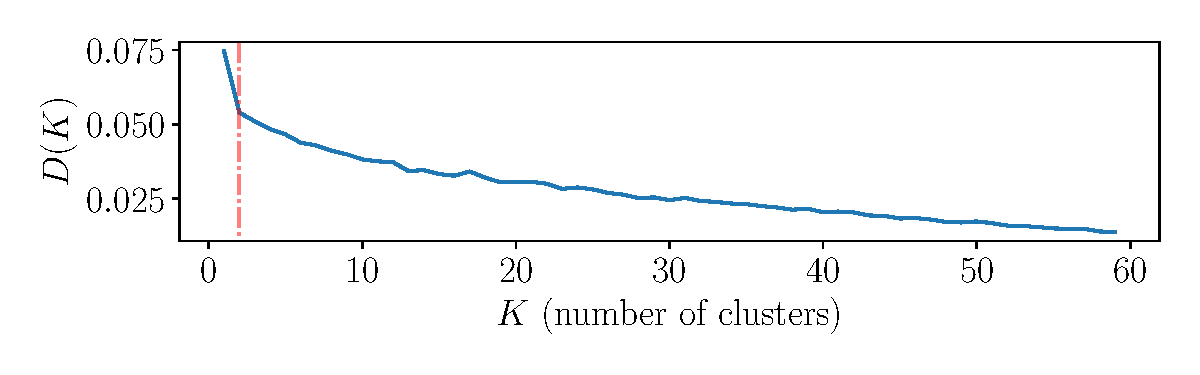
\includegraphics[width=0.8\textwidth]{capital_k.pdf}
	\caption{Capital budgeting. $D(K)$ vs. $K$. Dotted red line: $K = 2$.}%
	\label{fig:capitalk}%
\end{figure}
\begin{figure}[h]%
	\centering
	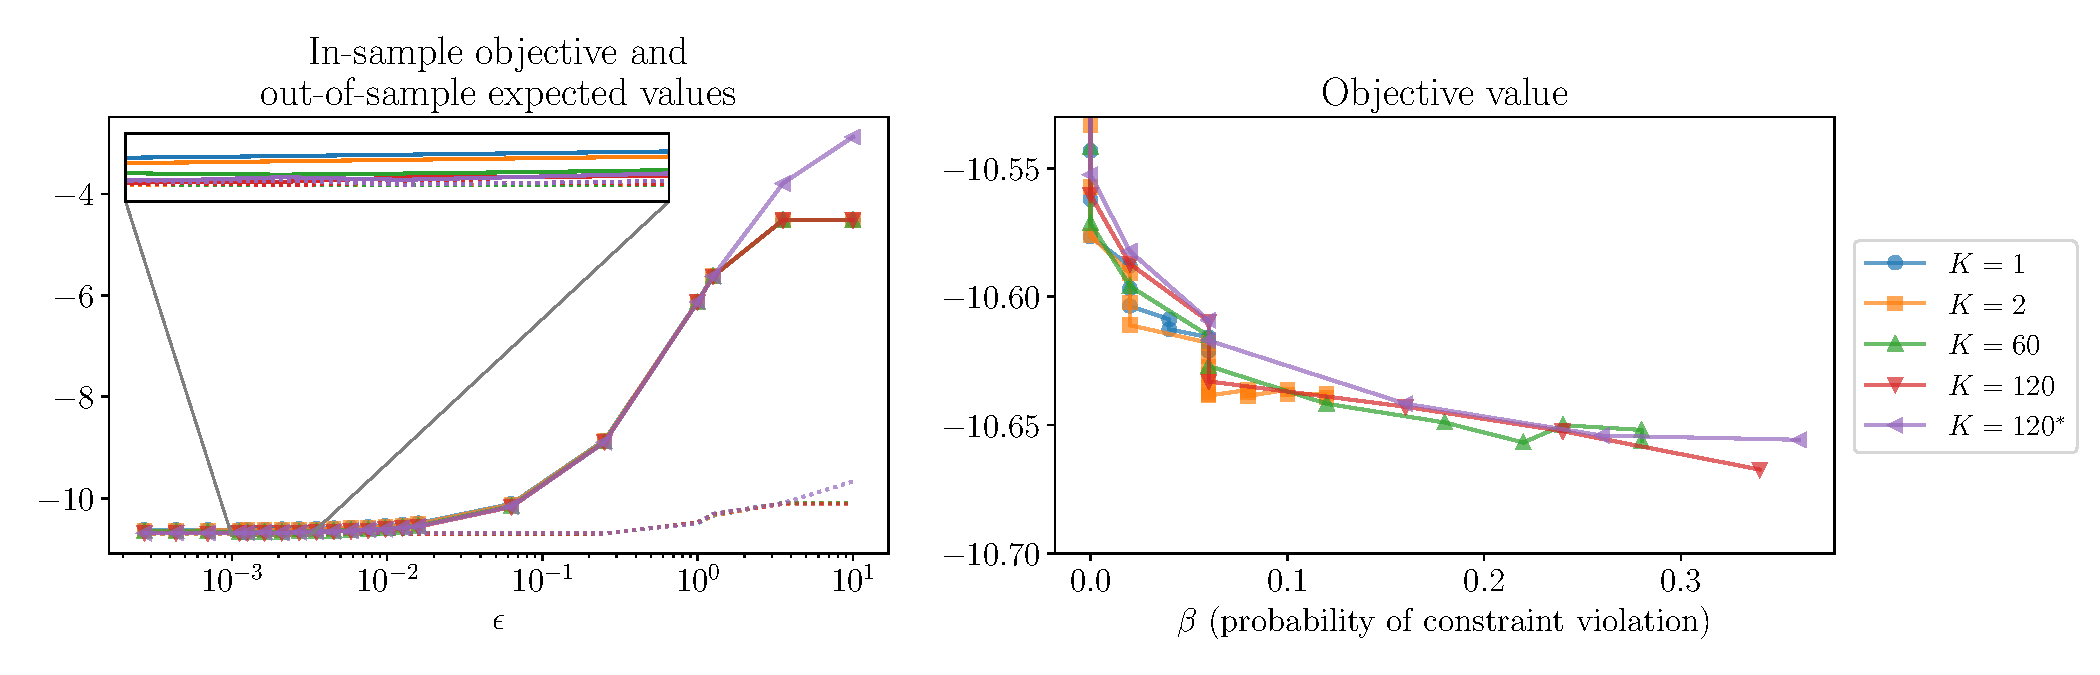
\includegraphics[width=\textwidth]{capitaltop2.pdf}
	\caption{Capital budgeting. Left: in-sample objective values and out-of-sample expected values vs. $\epsilon$ for different $K$. Solid lines are the in-sample objective value, dotted lines are the out-of-sample expected value. Right: objective value vs. $\beta$ for different $K$; each point represents the solution for the $\epsilon$ achieving the smallest objective value. $K = 120^*$ is the formulation without the support constraint. }%
	\label{fig:capital1}%
\end{figure}
\begin{figure}[h]%
	\centering
	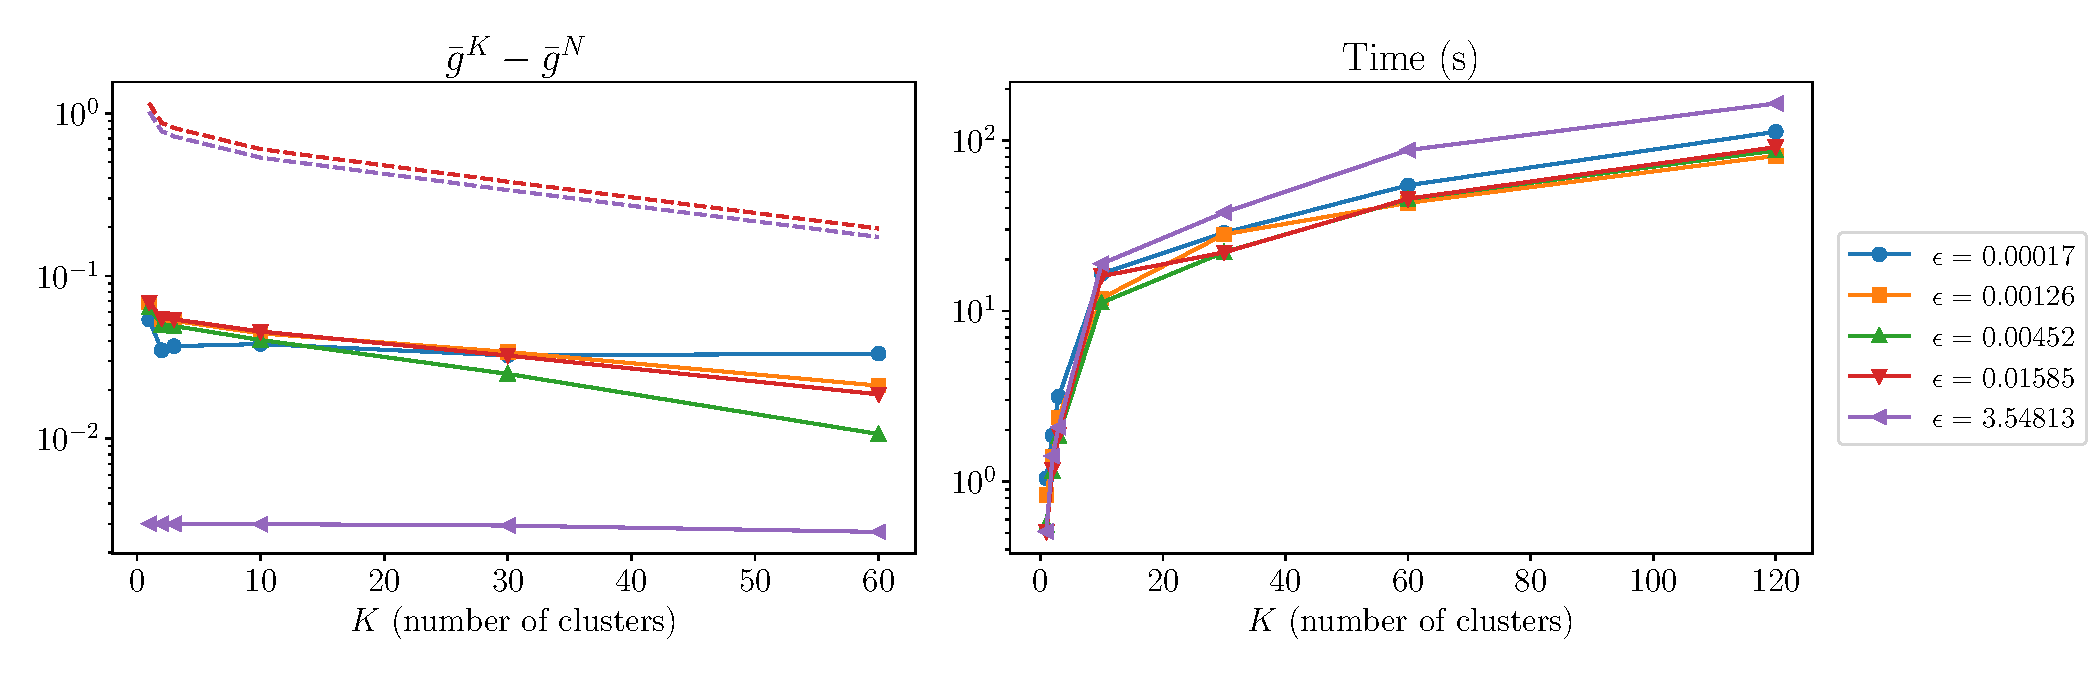
\includegraphics[width=\textwidth]{capitalbot2.pdf}
	\caption{Capital budgeting. Left: the difference in the value of the uncertain objective between using $K$ and $N$ clusters, calculated as $\bar{g}^K(z) - \bar{g}^N(z)$, compared with the theoretical upper bound $(L/2)D(K)$ from Corollary~\ref{cor:obj_unc}. Solid lines are the difference, dotted lines are the upper bounds. Right: solve time. }%
	\label{fig:capital2}%
\end{figure}

\paragraph{Results.}  We observe in Figure~\ref{fig:capital1} that using two clusters is enough to achieve performance almost identical to that of using 120 clusters.
Although from the left image, we see that $K=2$ slightly upper bounds $K = 120$, from the right, their tradeoffs between the objective value and relevant constraint violation probability ($\beta \leq 0.2$) are largely the same, so we can always tune $\epsilon$ to achieve the same performance and guarantees.
Notice that the results for $K = 120$ and $K=120^*$ are near identical for small $\epsilon$, where $K=120^*$ is the formulation without the support constraint. Therefore, while $ \bar{g}^{N*}(z)$ slightly upper bounds $\bar{g}^N(z)$, we can approximate their difference $\Delta \approx 0$ for small enough $\epsilon$, for which the upper bound $(L/2)D(K)$ thus hold.
In fact in this example, even for larger $\epsilon$ where we observe $\Delta > 0$, the actual difference between $\bar{g}^K$ and $\bar{g}^N$ is bounded by $(L/2)D(K)$.
\reviewChanges{
In Figure~\ref{fig:capital2}, we see that the elbow of the upper bound is at $K = 2$, and the true difference follows the same trend, matching the suggestion from Figure~\ref{fig:capitalk}.}
Therefore, setting $K = 2$ is the optimal decision, with a time reduction of 2 orders of magnitude, and a complexity reduction from 26626 variables and 12000 power cones to 666 variables and 200 power cones.



\subsection{Quadratic concave uncertainty}
\label{sub:quadraticconcave}
We refer to the example from Ben-Tal et al.~\cite[Section 4.2]{ben-tal_deriving_2015} with concave uncertainty of the form $$g(u,z) = \sum_{i=1}^n h_i(u) z_i,$$ where $h_i(u) = -(1/2)u^TA_iu$, each $A_i\in \reals^{m\times m}$ a symmetric positive definite matrix, $u \in \reals^m$, and $z \in \reals^{n}_{+}$. For simplicity, we also require that $z$ sums to 1, $p = 2$, and the support of the uncertainty $\supp = \reals^m$. Assuming the uncertainty is in the objective, such that the uncertain constraint is created using epigraph form, we solve the problem
\begin{equation*}
	\begin{array}{ll}
	\text{minimize} & \tau\\
	\text{subject to} & \lambda \epsilon^2 + \sum^{K}_{k=1} w_k s_k \leq \tau\\
	&(1/2)\sum_{i=1}^n \left({(Y_k)_i}^TA_i^{-1}(Y_{k})_i\right)/z_i -y_k^T\bar{d}_k  + 1/(4\lambda) \left\| y_k \right\|^2_2 \leq s_k \\
	&\hspace{7cm} \quad k = 1,\dots,K\\
& Y_{k}\ones = y_k, \quad k = 1,\dots,K\\
	& \ones^T z = 1, \quad \lambda \geq 0,\quad z \geq 0.
	\end{array}
\end{equation*}
The $A_i^{-1}$ terms come from taking the conjugate of $g$, and the derivation can be found in~\cite[Example 24]{ben-tal_deriving_2015}. We have variables $z \in \reals^n$, $y_k \in \reals^{m}$, $Y_{k} \in \reals^{m\times n}$, $\tau \in \reals$, $s_k \in \reals$, for $k= 1,\dots,K$. We let $(Y_k)_i$ indicate the $i$th column of $Y_k$.

\paragraph{Problem setup.}
We set $n = m = 10, N = 90$, and generate synthetic uncertainty as a multi-modal normal distribution with 5 modes, where $\mu_i = \gamma_j0.03i$ for all $i = 1,\dots, n$ for mode $j$, with mode scales $\gamma = (1, 5,15,25,40)$. The variance is $\sigma_i = 0.02^2 + (0.025i)^2$ for all modes. We generate $A_i$ as random positive semi-definite matrices for all $i = 1,\dots, n$. For the upper bound, we calulate $L = \|\sum_{i=1}^n A_i(\hat{z}_{N})_i\|_{2,2}$ for each data-driven solution $\hat{z}_N$.
\reviewChanges{
\paragraph{Choosing $K$}
Plotting the clustering value $D(K)$ over $K$, we note that the elbow occurs at $K=5$, which suggests a choice of $K=5$. }
\begin{figure}[h]%
	\centering
	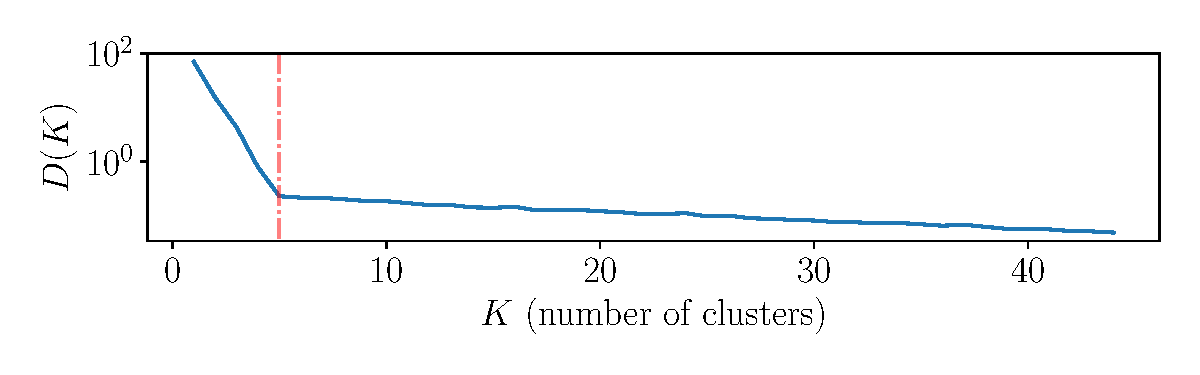
\includegraphics[width=0.8\textwidth]{quad_k.pdf}
	\caption{Quadratic concave uncertainty. $D(K)$ vs. $K$. Dotted red line: $K = 5$.}%
	\label{fig:concavek}%
\end{figure}
\begin{figure}[h]%
	\centering
	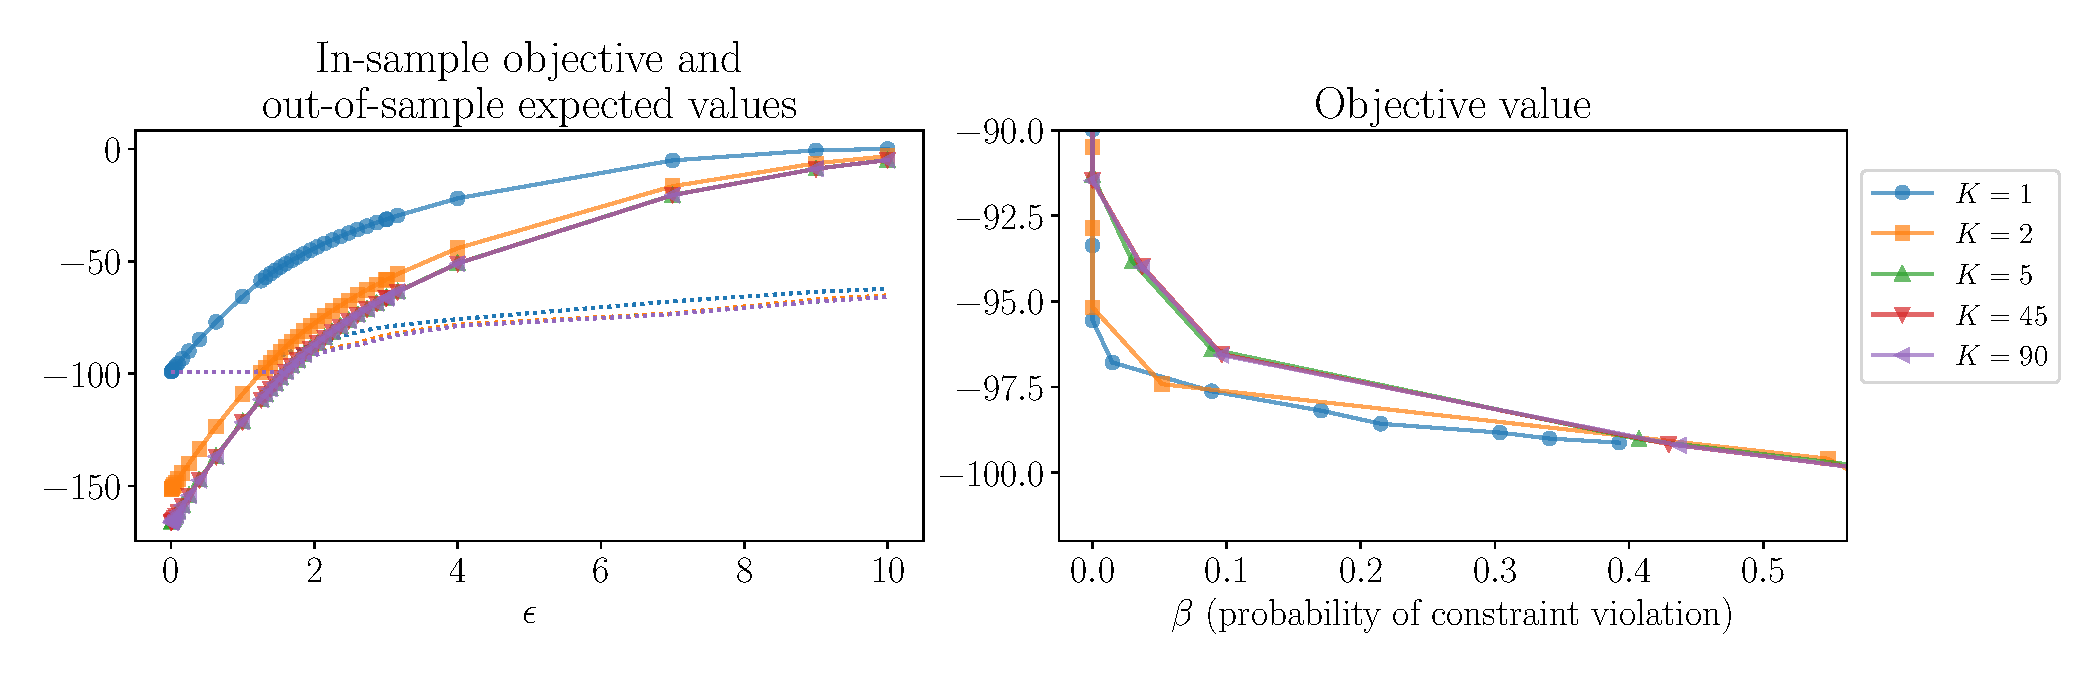
\includegraphics[width=\textwidth]{5modestop1.pdf}
	\caption{Quadratic concave uncertainty. Left: in-sample objective values and out-of-sample expected values of $g$ vs. $\epsilon$ for different $K$. Solid lines are the in-sample objective value, dotted lines are the out-of-sample expected value. Right: objective value vs. $\beta$ for different $K$; each point represents the solution for the $\epsilon$ achieving the smallest objective value. }%
	\label{fig:concave_syn1}%
\end{figure}
\begin{figure}[h]%
	\centering
	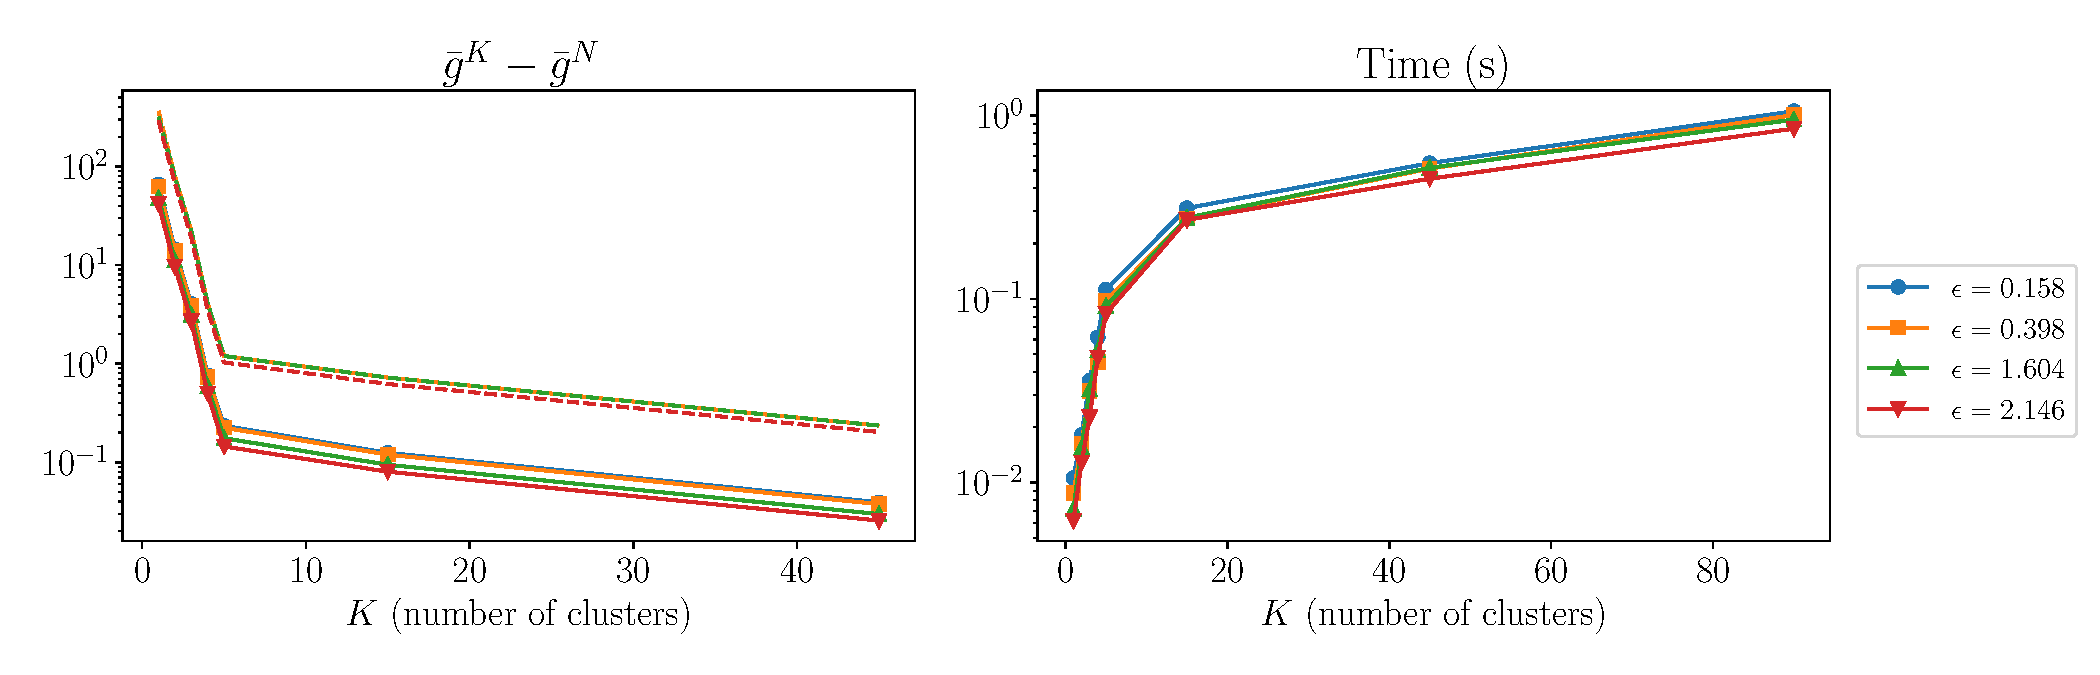
\includegraphics[width=\textwidth]{5modesbot1.pdf}
	\caption{Quadratic concave uncertainty. Left: the difference in the value of the uncertain objective between using $K$ and $N$ clusters, calculated as $\bar{g}^K(z) - \bar{g}^N(z)$, compared with the theoretical upper bound $(L/2)D(K)$ from Corollary~\eqref{cor:obj_unc}. Solid lines are the difference, dotted lines are the upper bounds. Right: solve time. }%
	\label{fig:concave_syn2}%
\end{figure}

\paragraph{Results.}  We observe on the left of Figure~\ref{fig:concave_syn1} that using 5 clusters is enough to achieve performance almost identical to that of using 90 clusters.
\reviewChanges{
Indeed, in Figure~\ref{fig:concave_syn2}, the elbow of the upper bound (dotted lines) on the difference in objective values is at $K = 5$, and the true difference follows the same trend, corroborating with Figure~\ref{fig:concavek}.}
Furthermore, on the left plot of Figure~\ref{fig:concave_syn2}, we note for $K \geq 5$, the tradeoff between the objective value and constraint violation is the same, so we can tune $\epsilon$ to achieve the same performance and guarantees.
In fact, for this particular example, using a smaller $K$ such as 1 or 2 may allow us to tune $\epsilon$ to achieve an even better tradeoff. However, this result cannot be guaranteed in general, so the recommended action is still to choose $K=5$.


\subsection{Robust log-sum-exp optimization}
\label{sub:logsumexp}
We also consider uncertainty from Bertimas and den Hertog~\cite[Chapter 14]{robustadaptopt} of the form
\begin{equation*}
	g(u,z) = \log\left(\sum_{i = 1}^n u_i e^{z_i}\right),
\end{equation*}
concave in $u$ and convex in $z$. This function $g$ is monotonically increasing in $u$, and we can define a domain $u \geq 0.01$ so that Assumption~\ref{assp:dom} and Theorem~\ref{thm:1} apply.
Assuming the simple case where the uncertainty is in the objective, we add some further restrictions on $z$ and use a cutting plane procedure to solve, for $p = 2$,
\begin{equation*}
	\begin{aligned}
	\underset{z}{\text{minimize}} \hspace{0.5em} \underset{u_1\dots u_k}{\text{maximize}} &\quad \sum_{k=1} ^K w_k  \log\left(\sum_{i = 1}^n u_i e^{z_i}\right) \\
	\mbox{subject to} & \quad \sum_{k=1} ^K w_k \| u_k - \bar{d}_k \|^2 \le \epsilon^2\\
	&\quad   \ones^T z \geq 10, \quad z \geq 0, \quad z \leq 10
	\end{aligned}
\end{equation*}
\paragraph{Problem setup.} We set $n = 30, N = 90$, and observe synthetic data from 3 sets of uniform distributions, scaled respectively by $\gamma = (1,3,7)$. Specifically, for each set $j$, each $d_i$ is generated uniformly on the intervals $0.01[\gamma_ji,\gamma_j(i+1)]$ for $i = 1,\dots, n$. For the upper bound, we calculate $L = \|\nabla^2 g\|_{2,2} \leq \exp(\hat{z}_N)^T\exp(\hat{z}_N)\min({d_k}^T\exp(\hat{z}_N))^{-2}$, for each data-driven solution $\hat{z}_N$.
\reviewChanges{
\paragraph{Choosing $K$}
Plotting the clustering value $D(K)$ over $K$, we note that the elbow occurs at $K=3$, which suggests using cross-validation for $K$ values around 3. }
\begin{figure}[h]%
	\centering
	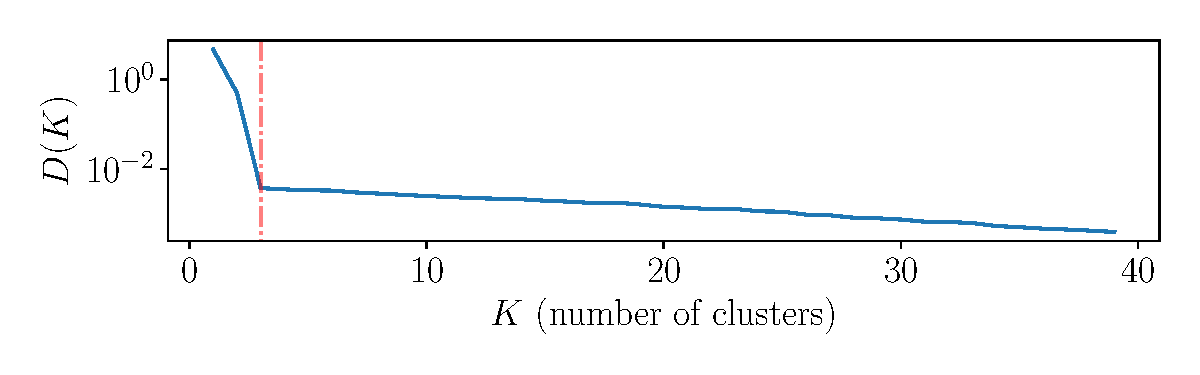
\includegraphics[width=0.8\textwidth]{log_k.pdf}
	\caption{Log-sum-exp uncertainty. $D(K)$ vs. $K$. Dotted red line: $K = 3$.}%
	\label{fig:logk}%
\end{figure}
\begin{figure}[h]%
	\centering
	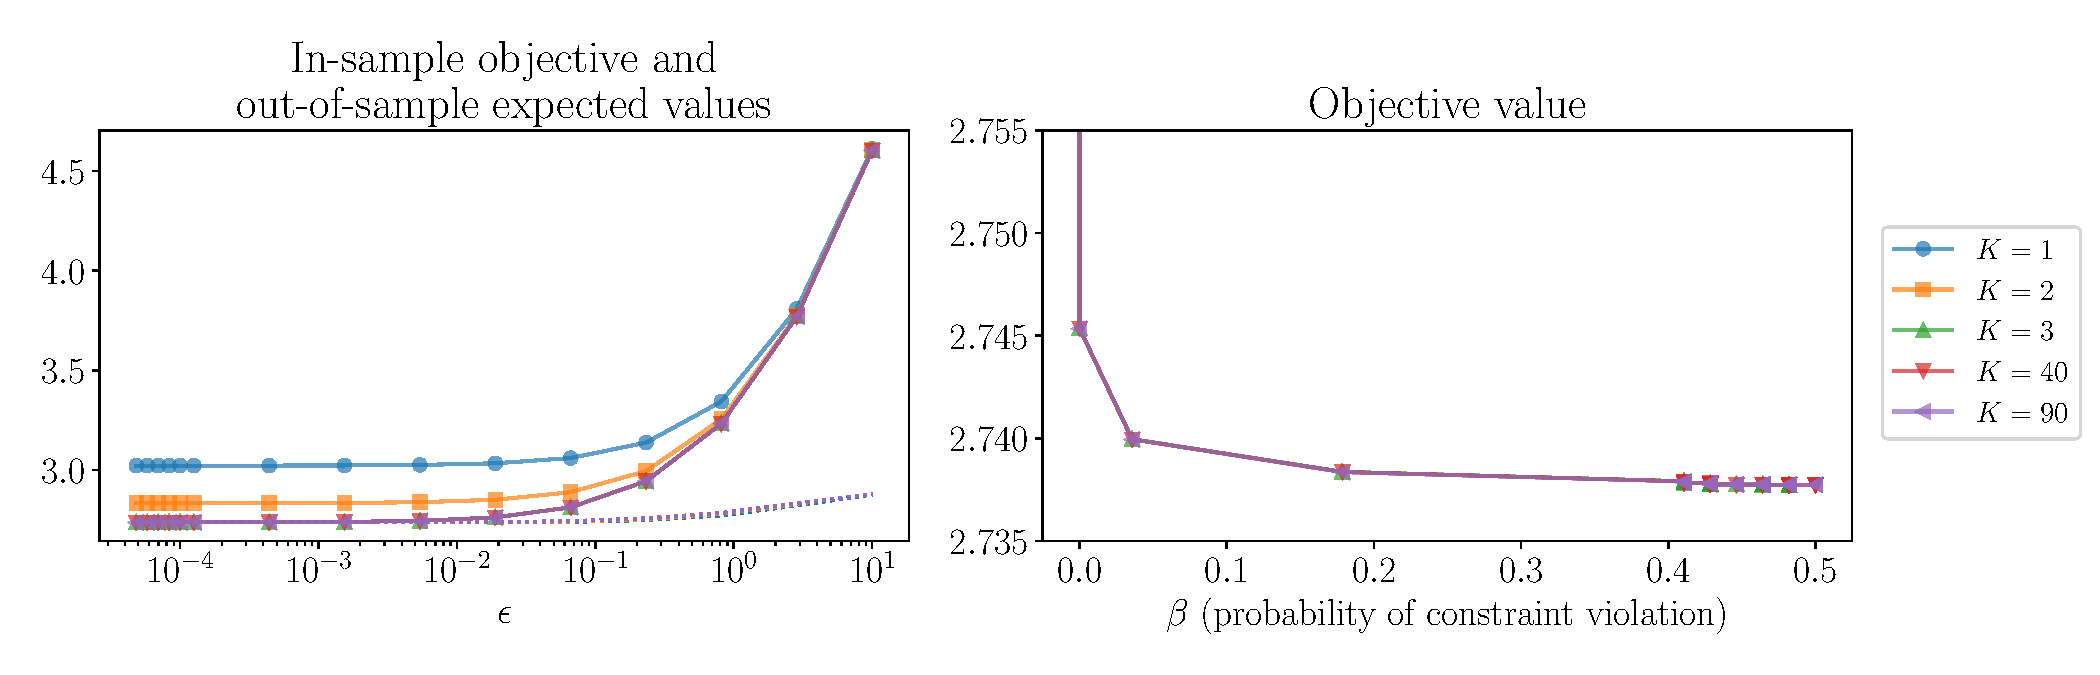
\includegraphics[width=\textwidth]{logtop2.pdf}
	\caption{Log-sum-exp uncertainty. Left: in-sample objective values and out-of-sample expected values vs. $\epsilon$ for different $K$. Solid lines are the in-sample objective value, dotted lines are the out-of-sample expected value. Right: objective value vs. $\beta$ for different $K$. }%
	\label{fig:log_syn1}%
\end{figure}

\begin{figure}[h]%
	\centering
	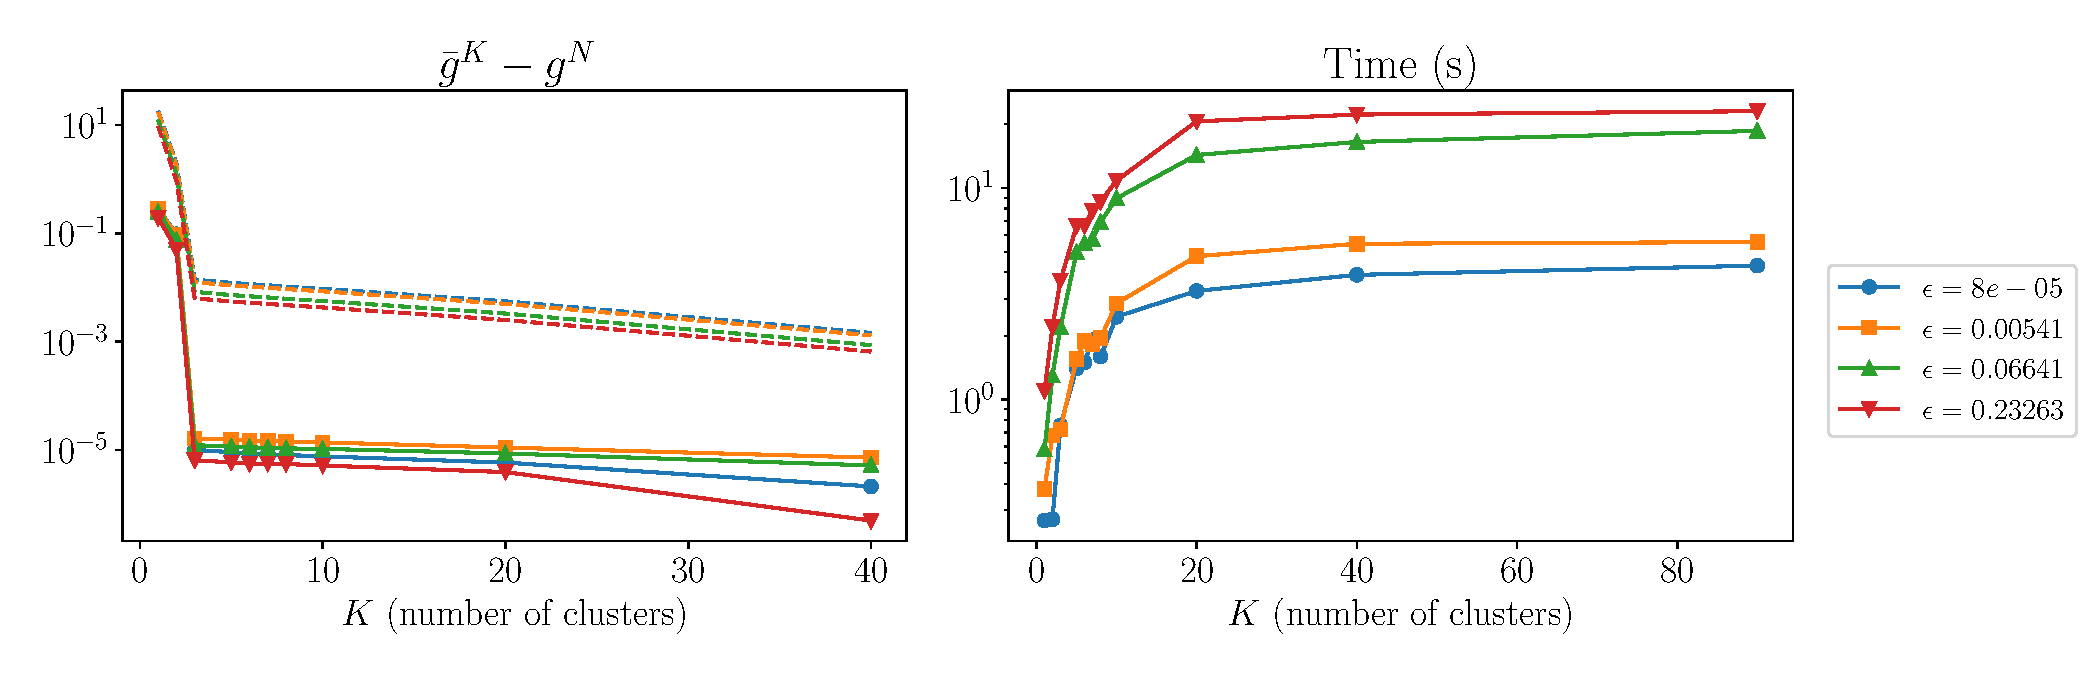
\includegraphics[width=\textwidth]{logbot.pdf}
	\caption{Log-sum-exp uncertainty. Left: the difference in the value of the uncertain objective between using $K$ and $N$ clusters. Solid lines are the difference, the dotted line is the upper bound. Right: solve time. }%
	\label{fig:log_syn2}%
\end{figure}

\paragraph{Results.} We observe on the left of Figure~\ref{fig:log_syn1} that while setting $K$ to smaller values increases the objective value, setting $K = 3$, the number of modes of the underlying distribution, already offers near identical performance to that of setting $K = 90$.
\reviewChanges{On the left of Figure~\ref{fig:log_syn2}, we see that $K = 3$ is at the elbow of upper bound and actual difference, corroborating with Figure~\ref{fig:logk}.}
Furthermore, we note that setting $K=3$ and above give identical tradeoff curves, therefore, choosing $K=3$ is the time-efficient solution.


\subsection{\reviewChanges{Sparse portfolio optimization}}%
\label{sub:sparse_portfolio_optimization}
\reviewChanges{
We consider a market that forbids short-selling and has $m$ assets as in~\citep{mohajerin_esfahani_data-driven_2018}.
Daily returns of these assets are given by the random vector $d = (d_1, \dots, d_m) \in \reals^m$.
The percentage weights (of the total capital) invested in each asset are given by the decision vector ${z = (z_1, \dots, z_n) \in \reals^n}$.
We restrict our selection to at most $\theta$ assets.
The underlying data-generating distribution $\prob$ is unknown, but we have observed a historical dataset  $\mathcal{D}_N$.
Our objective is to minimize the CVaR with respect to variable $z$,
\begin{equation*}
	\label{eq:portfolio}
	\begin{array}{ll}
	\text{minimize  } &\CVaR(- u^Tz,\alpha)\\
	\text{subject to} & \ones^T z = 1\\
			  & z \ge 0, \quad \|z\|_1 \leq \theta,
	\end{array}
\end{equation*}
which represents the average of the $\alpha$ largest portfolio losses that occur. In other words, the $\CVaR$ term seeks to ensure that the expected magnitude of portfolio losses, when they occur, is low.
The objective has an analytical form with an extra variable $\tau$ given as~\citep{cvaropt,mohajerin_esfahani_data-driven_2018}:
\begin{equation*}
	\text{minimize} \quad \Expect^{\prob}\left(\tau +\frac{1}{\alpha} \max\{-u^Tz -\tau, 0\}\right).
\end{equation*}
From this, we obtain $g$ as the maximum of affine functions,
\begin{equation*}
	g(u,z) \define \max\{(-1/\alpha)z^Tu + (1 - 1/\alpha)\tau, \tau \}.
\end{equation*}
Using the formulation~\eqref{eq:unif-dual-p} with $p= \infty$, we can write a convex reformulation of the form
\begin{equation*}
	\label{eq:portfolio_1}
	\begin{array}{ll}
	\text{minimize } & h\\
	\text{subject to } & \epsilon \left\|(1/\alpha)z\right\|_2 + \sum^{K}_{k=1} w_k s_k \leq h\\
	&  (1 - 1/\alpha)\tau - (1/\alpha)z^T\bar{d}_k    \leq s_k,\quad k = 1,\dots,K\\
	&  s_k \geq \tau, \quad k = 1,\dots,K\\
	& z \geq 0, \quad \mathbf{1}^T z = 1\\
	& y \in \{0,1\}, \quad y - z \leq 0, \quad \ones^Ty \leq \theta.
	\end{array}
\end{equation*}
with variables $z \in \reals^m$, $y \in \reals^m$, $h \in \reals$, $\tau \in \reals$, $s_k \in \reals$. The variables $y$ are introduced to replace the cardinality constraint using big-$M$ formulation~\citep{sparseportfolio}.}
\reviewChanges{
\paragraph{Problem setup.} We take stock data from the past 10 years of S\&P500, and generate synthetic data from their fitted general Pareto distributions.
We choose a generalized Pareto fit over a normal distribution as it better models the heavy tails of the returns~\citep{tails}.
See the Github repository for the code, which uses the "Rsafd" R package~\cite{Rsafd}.
We let $\alpha = 20\%$, $m = 50$ stocks, and generate a dataset size of $N = 1000$. Our portfolio can include at most $\theta = 5$ stocks. For the upper bound $\delta(K,y,\gamma)$ on $\bar{g}^N(z)-\bar{g}^K(z)$, we note the special structure of this problem, where one of the affine pieces is independent of $u$, to arrive at a bound $\delta(K,y,\gamma) = \max_k\{\max_i\{(\bar{d}_k - d_i)^Tz/\alpha\}\}$.}

\reviewChanges{
\paragraph{Choosing $K$}
Plotting the clustering value $D(K)$ over $K$, we note that the elbow occurs at $K=5$, which suggests using cross-validation for $K$ values around 5.}
\begin{figure}[h]%
	\centering
	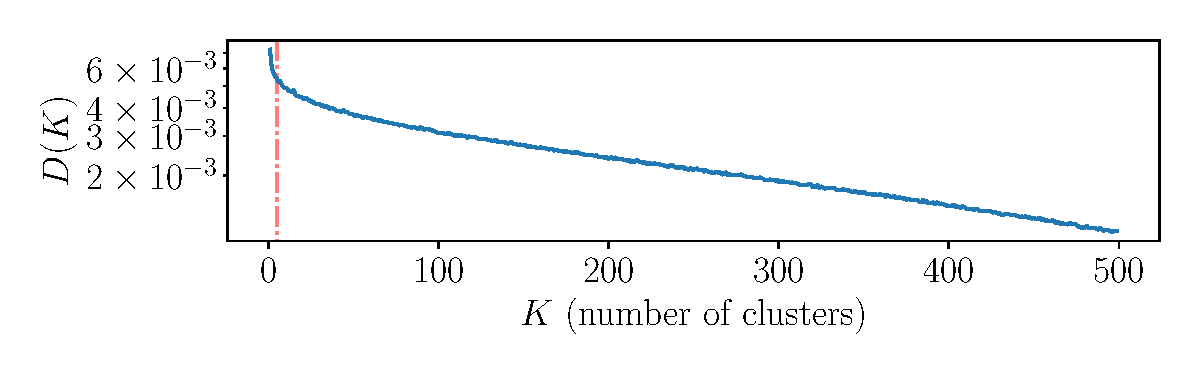
\includegraphics[width=0.8\textwidth]{port_k.pdf}
	\caption{Sparse portfolio. $D(K)$ vs. $K$. Dotted red line: $K = 5$.}%
	\label{fig:portk}%
\end{figure}

\reviewChanges{
\paragraph{Results.}%
In Figure~\ref{fig:portfolio1}, while setting $K$ to smaller values lead to a decrease in the optimal value across $\epsilon$, we note that for $K=5$ and above, we can already achieve a tradeoff curve between the optimal value and probability of constraint satisfaction that is similar to that of $K = 1000$, and setting $K=10$ brings it slightly closer. In Figures~\ref{fig:portk} and~\ref{fig:portfolio2}, in the plots of $D(K)$ and of the upper bound on the difference, we also note that the elbow is around $K=5$. We thus recommend choosing $K$ through cross validation around 5, as tuning $\epsilon$ for these small $K$ gives 1 - 3 orders of magnitude time reduction.}

\begin{figure}[h]%
	\centering
	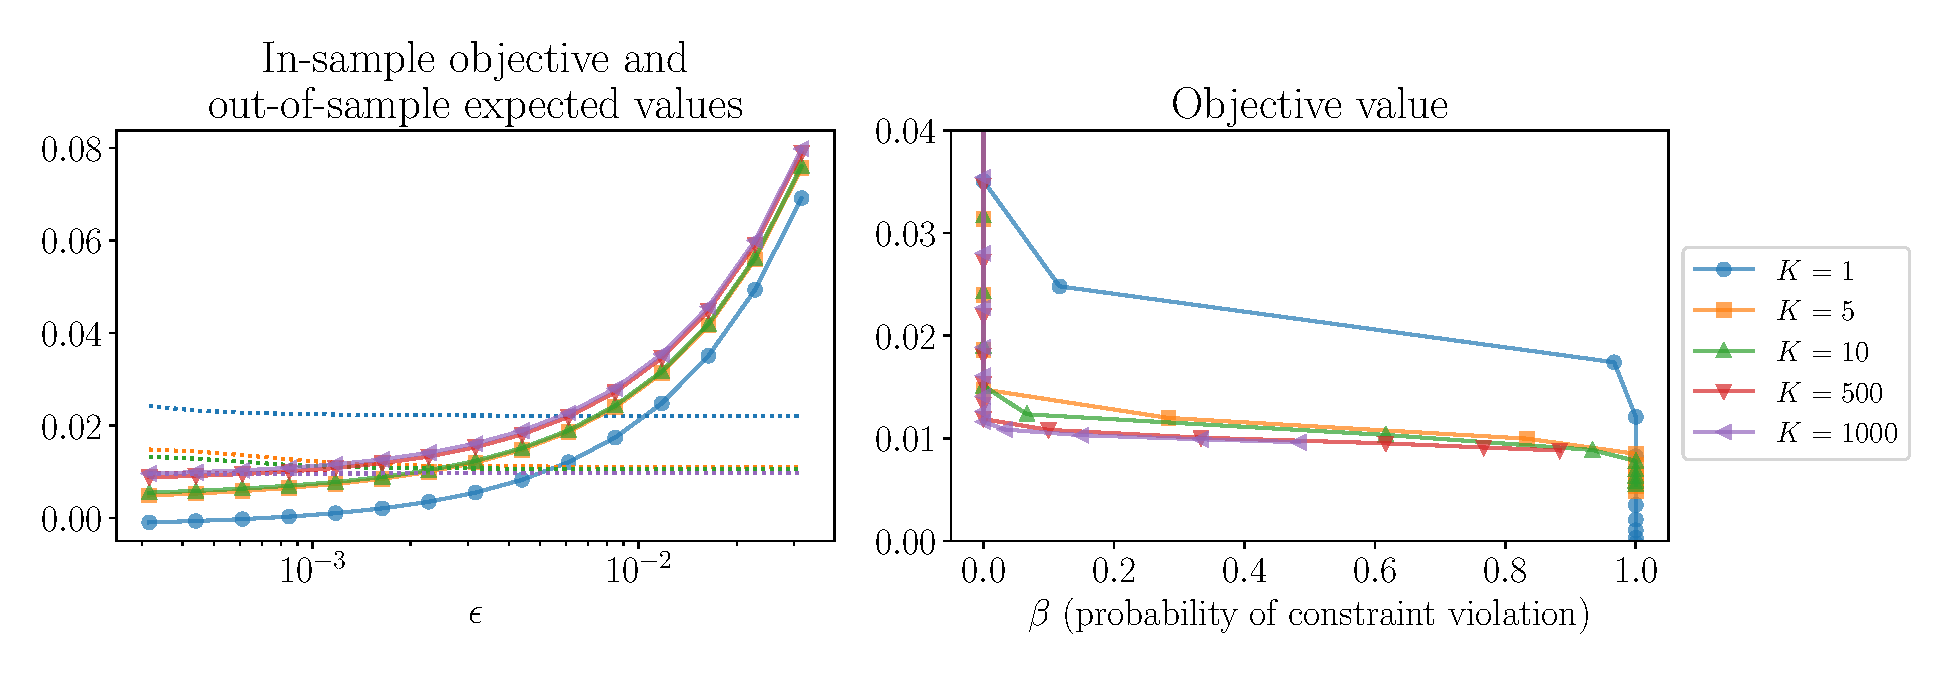
\includegraphics[width=\textwidth]{portMIPtop.pdf}
	\caption{Sparse portfolio. Left: in-sample objective values and out-of-sample expected values vs $\epsilon$ for different $K$. Solid lines are the in-sample objective value, dotted lines are the out-of-sample expected value. Right: objective value vs $\beta$ for different $K$; each point represents the solution for the $\epsilon$ achieving the smallest objective value.}%
	\label{fig:portfolio1}%
\end{figure}
\begin{figure}[h]%
	\centering
	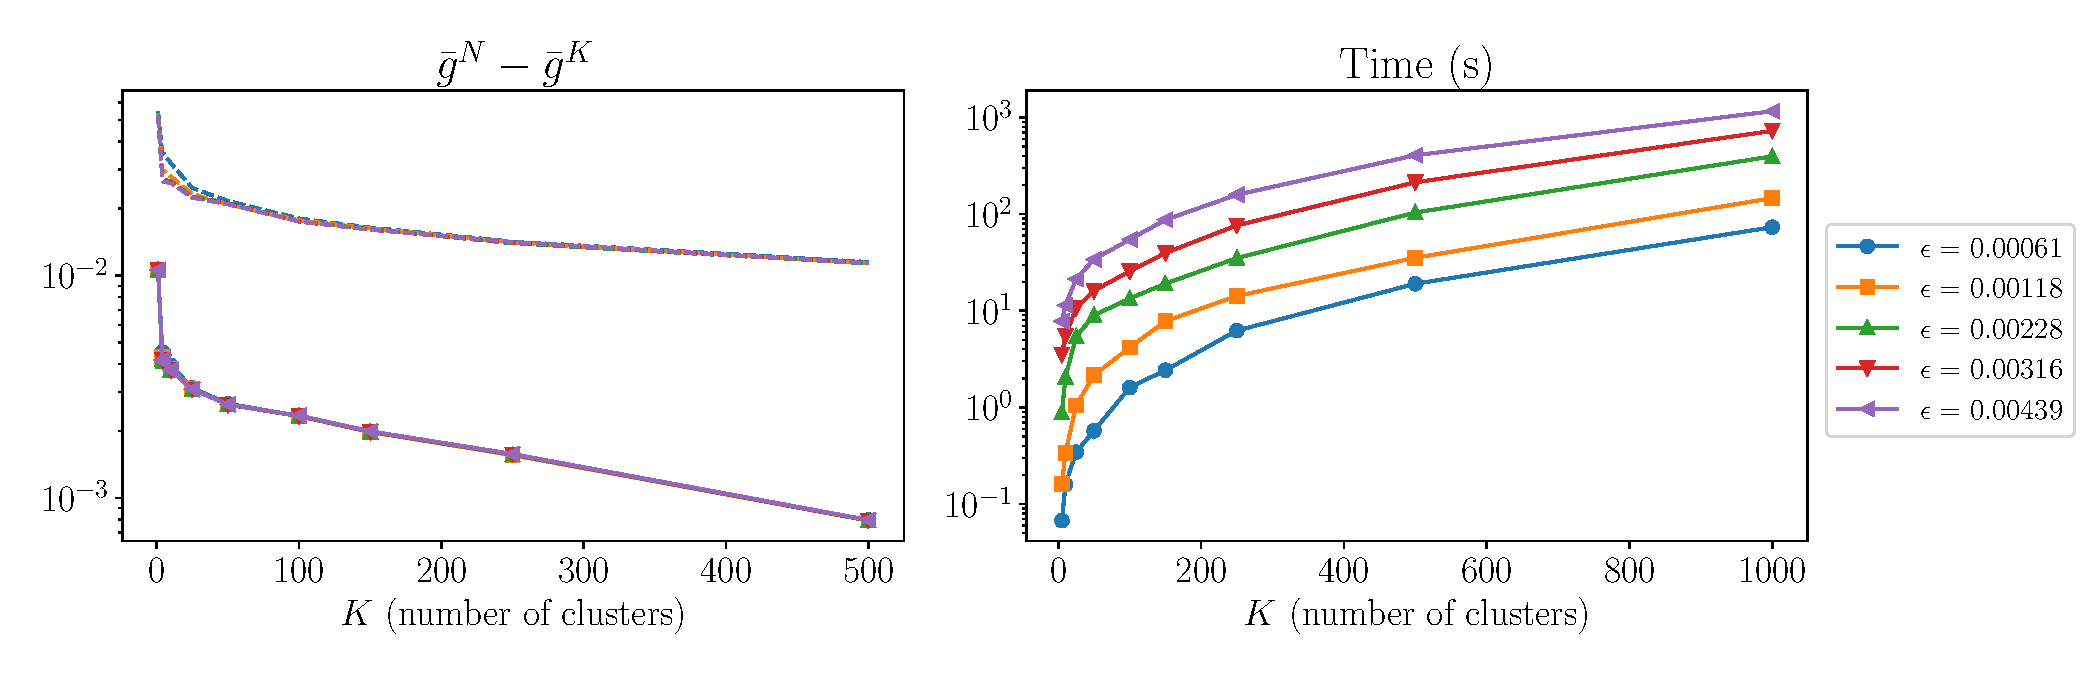
\includegraphics[width=\textwidth]{portMIPbot.pdf}
	\caption{Sparse portfolio. Left: the difference in the value of the uncertain objective between using $N$ and $K$ clusters, calculated as $\bar{g}^N(z) - \bar{g}^K(z)$, compared with the theoretical upper bound $\delta(K,y,\gamma)$ from Corollary~\ref{cor:maxaffine}. Solid lines are the difference, dotted lines are the upper bounds. Right: solve time for $K \geq 5$. }%
	\label{fig:portfolio2}%
\end{figure}


\subsection{Facility location}
\label{sub:facility}
We examine the classic facility location problem~\citep{bertsimas_probabilistic,HOLMBERG1999544}.
Consider a set of $n$ potential facilities, and $m$ customers.
Variable $z \in \{0, 1\}^n$ describes whether or not we construct each facility $i$ for $i=1, \dots, n$,  with cost $c_i$.
In addition, we would like to satisfy the uncertain demand $u\in \reals^m$ at minimal cost.
We define variable $X\in\mathbf{R}^{n\times m}$ where $X_{ij}$ corresponding to the portion of the demand of customer $j$ shipped from facility $i$ with corresponding cost $C_{ij}$.
Furthermore, $r \in \reals^n$ represents the production capacity for each facility, and $u\in \reals^m$ represents the uncertain demand from each customer.
For each customer $j$, $X_j$ represents the proportion of goods shipped from any facility to that customer, which sums to $1$.
For each facility $i$, $(X^T)_i$ represents the proportion of goods shipped to any customer.
Putting this all together, we obtain multiple affine uncertain capacity constraints,
\begin{equation*}
	g_i(u,z) \define (X^T)_i u - r_i z_i \leq 0 \quad i = 1,\dots,n,
\end{equation*}
\reviewChanges{which we combine to create a single maximum-of-affine constraint,
\begin{equation*}
	g(u,z) \define \max_{i \leq n}((X^T)_i u - r_i z_i) \leq 0.
\end{equation*}
Now, to ensure a high probability of constraint satisfaction, we use the $\CVaR$ reformulation, 
\begin{equation*}
	g(u,z,\tau) \define \tau + (1/\alpha)\max \left (\max_{i \leq n}((X^T)_i u - r_i z_i - \tau), 0\right ) \leq 0,
\end{equation*}
where we add the auxiliary variable $\tau$. We assume a polyhedral support $\supp= \{u \mid Hu\leq b\}$ for the demand, and solve the problem, for $p = \infty$,
\begin{equation*}
	\label{eq:mro_facility_mip_ref}
	\begin{array}{ll}
	\text{minimize} & c^Tz  +\Tr(C^TX)\\
	\text{subject to}  &\ones^TX_j = 1,\quad j = 1,\dots, m \\
	&   \tau + \sum_{k=1}^K w_k s_{k}  \leq 0,\\
	 & -(1/\alpha)\tau + \lambda_{k} \epsilon + (1/\alpha)((X^T)_i\bar{d}_k -r_ix_i) + \gamma_{ik}(b - H\bar{d}_k) \leq s_{k},\\
	 &\hspace{4cm} \quad i = 1,\dots,n, \quad k = 1,\dots, K\\
	 & \lambda_{k} \epsilon  \leq s_{k}, \quad k = 1,\dots, K\\
	 & \left\| H^T\gamma_{ik} + (1/\alpha)(X^T)_i\right\|_2 \leq \lambda_{k}, \quad i = 1,\dots,n, \quad k = 1,\dots, K\\
	 & \gamma_{ik} \geq 0, \quad i = 1,\dots,n, \quad k = 1,\dots, K\\
	 & z\in \{0,1\}^n, \quad X\in \reals^{n\times m}.
	\end{array}
\end{equation*}
We have variables $z \in \{0,1\}^{n}$, $X \in \reals^{n\times m}$, $s_{k} \in \reals$, $\tau \in \reals$, $\lambda_k \in \reals$, $\gamma_{ik} \in \reals^{m}$, for $i = 1,\dots,n$ and $k= 1,\dots,K$.
The $\gamma$ variables arise from enforcing the support constraints.}

% Even though we obtain a probabilistic guarantee of the form~\eqref{eq:robustopt-sep-g}, which can be interpreted as a separate probabilistic guarantee for each facility, we can still tune $\epsilon$ to obtain the stricter guarantee
% \begin{equation}
% 	\label{eq:robustopt-g}
%     \prob^N \bigg({\Expect}^{\prob}\left(\underset{l}{\max}\;g_l(u,\hat{x}_N)\right)\leq 0 \bigg) \geq 1- \beta,
% \end{equation}
% which guarantees that the uncertain constraints for all facilities are satisfied simultaneously.

\paragraph{Problem setup.}%
To generate data, we set $n = 5$ facilities, $m = 25$ customers, and $N = 50$ data samples.  \reviewChanges{For the $\CVaR$ reformulation, we set $\alpha = 20\%$. We set costs $c = (46.68, 58.81, 30, 42.09, 35.87)$, and generate the two coordinates of each customer's location from a uniform distribution on $[0,15]$. We then calculate $C$ as the $\ell_2$ distance between each pair of customers. We set production capacities $r = (33, 26, 41, 26, 22)$.
We assume the demand $d$ is supported between 1 and 6, which we write as $Hu\leq b$, where $H = [-I\; I]^T$ and $b$ is the concatenation of two vectors: a vector of $-1$'s of length $m$, and a vector of $6$'s of length $m$. 
We generate demands as the combination of two normal distributions. Half of the data is generated from the normal distribution with mean $\mu_1 = 3$ and variance $\sigma_1 = 0.9$, the second half has mean $\mu_1 = 4$ and variance $\sigma_1 = 0.8$.
We then project the demands onto $(1,6)$.}
% Since the underlying distribution is uniform, it satisfies the assumptions of Theorem~\ref{theorem-inf}, so theoretical guarantees also exist for $p = \infty$. 
\reviewChanges{For the upper bound $\delta(K,y,\gamma)$ on  $\bar{g}^N(z) - \bar{g}^K(z)$ from Corollary~\ref{cor:maxaffine}, we have $(1/N)\sum_{k=1}^K \sum_{i \in C_k}  \max(\max_{j\leq J}((X[i] -H^T\gamma_{jk}),0)^T(d_i - \bar{d}_k))$. Note that this upper bounds the difference in constraint values, and only indirectly affects the objective values through restrictions on the feasible region. Therefore, it is not an upper bound on the difference in objective value, merely a rough estimate.
We cannot directly compare this upper bound against the change in constraint values, as at the optimal chosen $z, X$ for each $K$, which differ due to differences in the feasible regions, the constraint value will always be near 0 for optimality. We thus compare it against the change in objective values. }
\reviewChanges{
\paragraph{Choosing $K$}
Plotting the clustering value $D(K)$ over $K$, we note that the elbow occurs at $K=2$, which suggests using cross-validation for $K$ values around 2. }
\begin{figure}[h]%
	\centering
	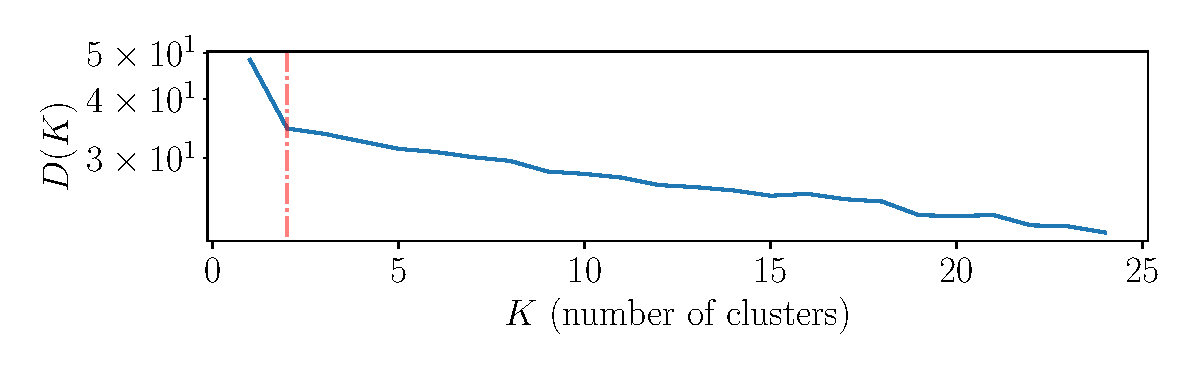
\includegraphics[width=0.8\textwidth]{facility_k.pdf}
	\caption{Facility location. $D(K)$ vs. $K$. Dotted red line: $K = 2$.}%
	\label{fig:facilityk}%
\end{figure}

% \begin{figure}[h]%
% 	\centering
% 	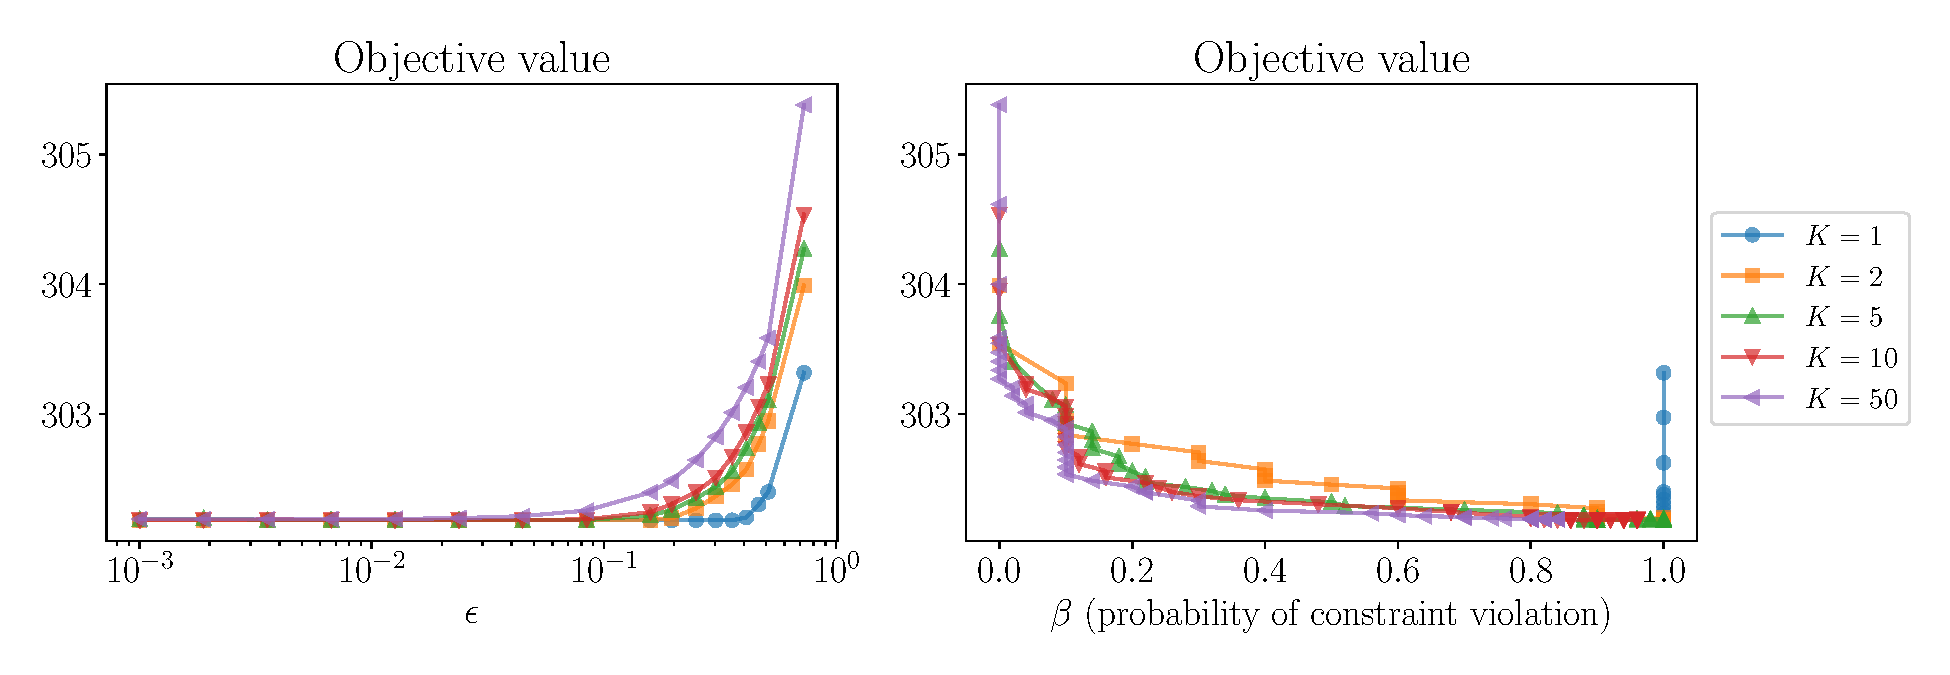
\includegraphics[width=\textwidth]{facilitytop.pdf}
% 	\caption{Facility location. Top left: in-sample objective values vs. $\epsilon$ for different $K$. Top right$^*$: $\epsilon$ vs. the original probabilitic guarantee~\eqref{eq:robustopt-sep-g} for different $K$. Bottom left$^{**}$: $\epsilon$ vs. the stricter probabilistic guarantee~\eqref{eq:robustopt-g}. Bottom right: solve time. $K=1^*$ is the formulation without the support constraint. }%
% 	\label{fig:facility}%
% \end{figure}
\paragraph{Results.}%
\reviewChanges{
As expected of maximum-of-affine $g$, we note in Figure~\ref{fig:facility} that setting $K$ to smaller values lead to a decrease in the optimal value across different $\epsilon$ values. 
While $K=1$ yields poor performance in terms of the probability of constraint violation, we observe that $K=2$ already yields a tradeoff between the objective and probability of constraint violation close to that of $K=50$. Through cross-validation with different $K$, we select $K=5$, which provides a tradeoff curve closer to optimality. 
As this problem has uncertainty in the constraints and not the objective, the bounds given in Corollary~\ref{cor:maxaffine} do not directly reflect the difference in the objective values. 
However, they do give a reference value and inform us of the general trend of the difference.
In this case, they still upper bound the actual difference, as shown in Figure~\ref{fig:facility}.
We note that the bounds we use do not depend on $\bar{g}^{N*}(z)$, so it is irrelevant whether or not the support has an affect on the worst-case constraint value.
Overall, choosing $K = 5$ leads to a time reduction of an order of magnitude while achieving near-optimal performance. 
}
\begin{figure}[h]%
	\centering
	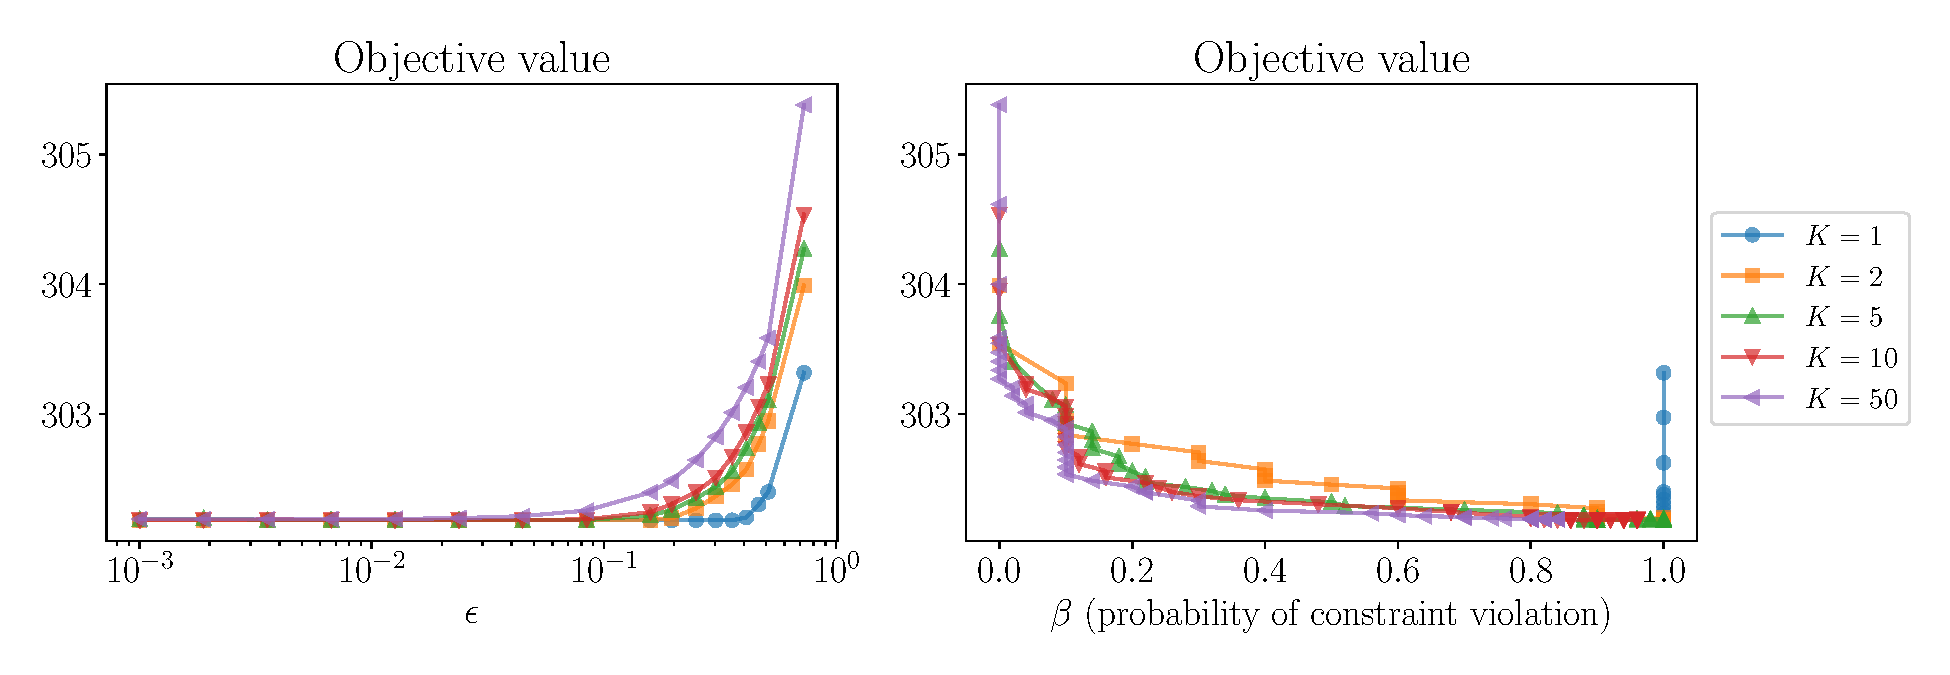
\includegraphics[width=\textwidth]{facilitytop.pdf}
	\caption{Facility location. Left: in-sample objective values vs $\epsilon$ for different $K$. Right: objective value vs $\beta$ for different $K$; each point represents the solution for the $\epsilon$ achieving the smallest objective value. }%
	\label{fig:facility}%
\end{figure}
\begin{figure}[h]%
	\centering
	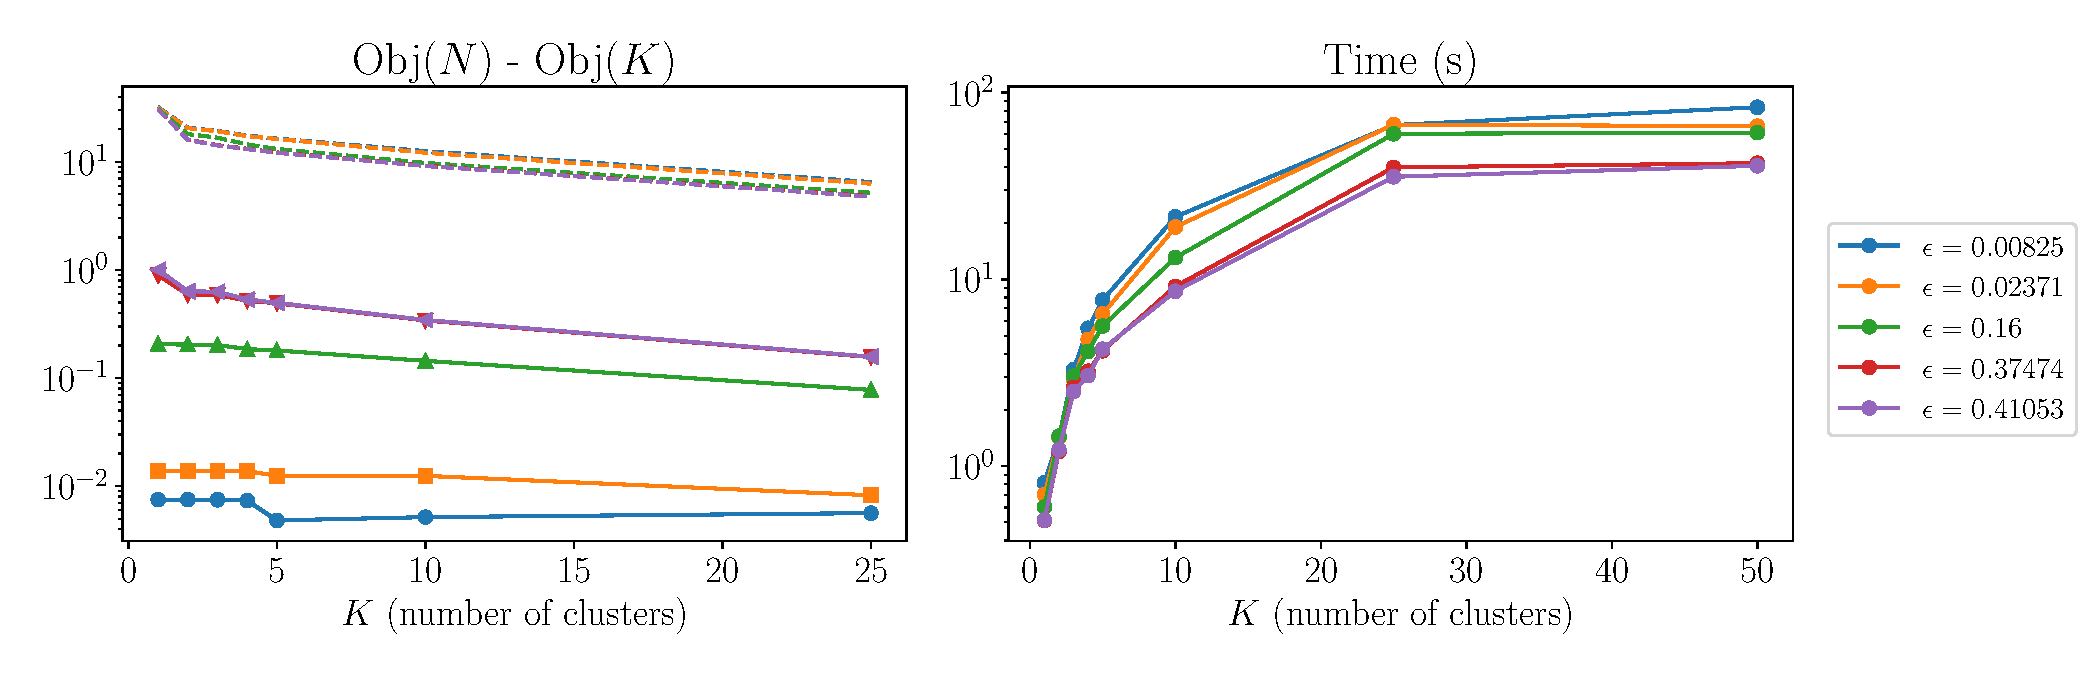
\includegraphics[width=\textwidth]{facilitybot1.pdf}
	\caption{Facility location. Left: the difference in the value of the uncertain objective between using $N$ and $K$ clusters, calculated as Obj($N$) - Obj($K$), compared with the theoretical upper bound $\delta(K,y,\gamma)$ on the worst-case constraint value $\bar{g}^N(z) - \bar{g}^K(z)$,  from Corollary~\ref{cor:maxaffine}. Solid lines are the difference, dotted lines are the upper bounds. Right: solve time. }%
	\label{fig:facility1}%
\end{figure}


\subsection{\reviewChanges{Newsvendor problem}}
\label{sub:news}
\reviewChanges{
We consider a 2-item newsvendor problem where, at the beginning of each day, the vendor orders $z\in \reals^2$ products at price $h=(4,5)$. These products will be sold at the prices $c=(5,6.5)$, until either the uncertain demand $u$ or inventory $z$ is exhausted.
The objective function to minimize is the sum of the ordering cost minus the revenue:
\begin{equation*}
	h^Tz - c^T\min\{z,u\},
\end{equation*}
from which we obtain the maximum-of-affine uncertain function $g$ to minimize,
$$g(u,z) = h^Tz + \max(-c_1z_1 - c_2 z_2, -c_1 z_1 -c_2 u_2, -c_1u_1 -c_2z_2, -c_1u_1 - c_2u_2 ).$$}
\reviewChanges{
We assume a polyhedral support $\supp= \{u \mid Cu\leq b\}$, and solve, with $p = 1$,
\begin{equation*}
	\label{eq:news}
	\begin{array}{ll}
	\text{minimize} & h^Tz  + \lambda\epsilon + \sum_{k=1}^K w_k s_{k} \\
	\text{subject to}  & -c^Tz + \gamma_{1k}^T(b - C\bar{d}_k)  \leq s{k}, \quad k = 1,\dots, K\\
	& -c_1 z_1 - \bar{d}_k^T(c_2e_2) + \gamma_{2k}^T(b - C\bar{d}_k) \leq s_k , \quad k = 1,\dots, K\\
& -c_2 z_2 - \bar{d}_k^T(c_1e_1) + \gamma_{3k}^T(b - C\bar{d}_k) \leq s_k, \quad k = 1,\dots, K\\
& -\bar{d}_k^T(c) + \gamma_{4k}^T(b - C\bar{d}_k) \leq s_k, \quad k = 1,\dots, K\\
	 & \left\| -C^T\gamma_{1k} \right\|_2 \leq \lambda_{k}, \quad k = 1,\dots, K\\
	 & \left\| -C^T\gamma_{2k}+ c_1 e_1 \right\|_2 \leq \lambda_{k}, \quad k = 1,\dots, K\\
	 & \left\| -C^T\gamma_{3k}+ c_2 e_2\right\|_2 \leq \lambda_{k}, \quad k = 1,\dots, K\\
	 & \left\| -C^T\gamma_{4k}+ c \right\|_2 \leq \lambda_{k}, \quad k = 1,\dots, K\\
	 & \gamma_{jk} \geq 0, \quad j = 1,\dots,4, \quad k = 1,\dots, K\\
	 & z \geq 0
	\end{array}
\end{equation*}
We have variables $z \in \reals^{n}$,$s_{k} \in \reals$, $\lambda \in \reals$, $\gamma_{jk} \in \reals^{m}$, for $j = 1,\dots,4$ and $k= 1,\dots,K$.
The $\gamma$ variables arise from enforcing the support. We denote $e_1 = (1,0)$ and $e_2 = (0,1)$.}

\reviewChanges{
For this problem, we consider the effects of outliers on the performance of \gls{MRO}. Therefore, we consider the data to have an outlier at $(0,0)$, the worst-case value of the support set. In Figure~\ref{fig:news}, we show a set of generated data along with this outlier point. }
\begin{figure}[h]%
	\centering
	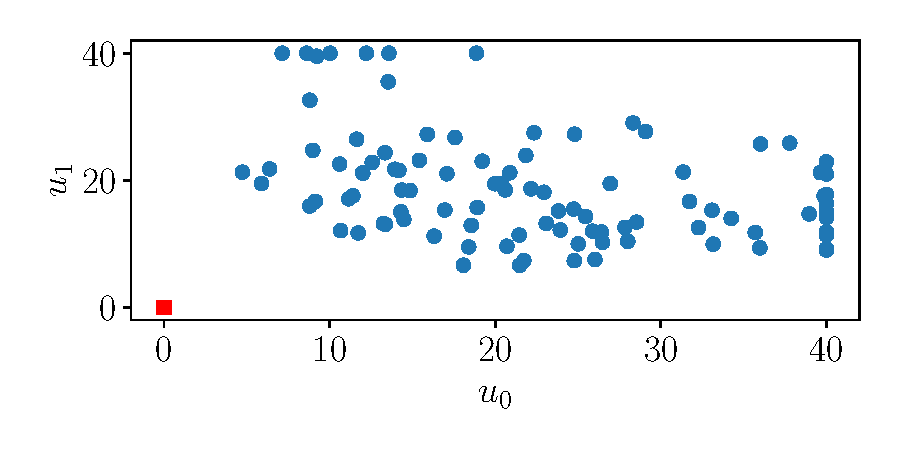
\includegraphics[width=0.6\textwidth]{news_outliers.pdf}
	\caption{Newsvendor. Datapoints and the outlier at (0,0). }%
	\label{fig:news}%
\end{figure}

\reviewChanges{
We consider three ways to solve the problem, decribed as follows. 
\begin{enumerate}
	\item \gls{MRO}, where we directly apply \gls{MRO} to the dataset with the outlier.
	\item ROB-\gls{MRO}, where we perform preliminary analysis on the dataset to remove the outlier point, then apply \gls{MRO} to the cleaned dataset. 
	\item AUG-\gls{MRO}, where we perform the clustering step on data without the outlier, then define an augmented distribution supported on $K+1$ points, where the extra point is the outlier point (0,0), with weight $1/N$. The weights of the other clusters are adjusted accordingly. 
\end{enumerate}}



\reviewChanges{
\paragraph{Problem setup.}%
To generate data, we set $N = 100$ data samples. We assume demand is supported between 0 and 40, which we write as $Cu\leq b$, where $C = [-I\; I]^T$ and $b = (0,0,0,0,40,40,40,40)$. We allow non-integer demand to allow for more variance in the data.
We generate the demand from a log-normal distribution, where the underlying normal distribution has parameters
\begin{equation*}
	\mu =
\left[ \begin{array}{l} 3.0 \\
2.8 \end{array} \right],\quad \Sigma =
\left[\begin{array}{ll} \phantom{-}0.3 & -0.1\\
-0.1 & \phantom{-}0.2 \end{array} \right],
\end{equation*}
and take the minimum between the generated values and 40. For the upper bound $\delta(K,y,\gamma)$ on  $\bar{g}^N(z) - \bar{g}^K(z)$ from Corollary~\ref{cor:maxaffine}, we have $(1/N)\sum_{k=1}^K \sum_{i \in C_k}  \max_{j\leq 4}((-\tilde{c}_j -C^T\gamma_{jk})^T(d_i - \bar{d}_k))$, where $\tilde{c}_1 = 0,~ \tilde{c}_2 = c_1e_1,~\tilde{c}_3 = c_2e_2,~\tilde{c}_4 = c$.}

\reviewChanges{
\paragraph{Choosing $K$}
Plotting the clustering value $D(K)$ over $K$, for the dataset both with and without the outlier, we note an elbow at around $K=5$, though not very prominent. The recommendation is setting $K$ around 5, to be fine tuned through cross-validation.}

\begin{figure}[h]%
	\centering
	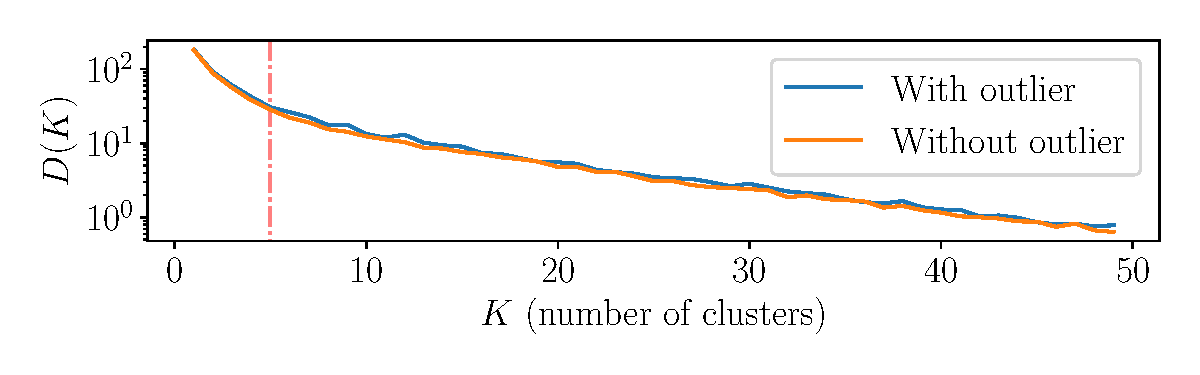
\includegraphics[width=0.8\textwidth]{news_k.pdf}
	\caption{Newsvendor. $D(K)$ vs. $K$. Dotted red line: $K = 5$.}%
	\label{fig:newsk}%
\end{figure}
\reviewChanges{
\paragraph{Results.}
In Figure~\ref{fig:news2}, we compare the in and out-of-sample objective values of the three methods, and note their similar performance. While setting $K=1$ yields suboptimal results, we note that for $K=5$ and above, we can achieve similar performance as setting $K=100$. To examine the effect of the outlier more closely, in Figures~\ref{fig:newscomp} and~\ref{fig:newscomp2}, we compare, for $K=10$ and $K=100$, the objectives and tradeoff curves for the three methods. We note that, when the outlier is averaged with other datapoints, the final in-sample objective may be improved, as the centroid moves closer to the non-outlier points. We observe this in Figure~\ref{fig:newscomp}, where \gls{MRO}, in which the outlier may be clustered with other points, offers a lower in-sample objective than AUG-\gls{MRO}, in which the outlier is considered its own cluster. \gls{MRO} has in fact offered protection against the outlier.  Lastly, as expected, ROB-\gls{MRO}, where the outlier point is removed, yields the best in-sample results. Regardless of the method, we note that the final out-of-sample tradeoff curves are near-identical. Comparing Figures~\ref{fig:newscomp} and~\ref{fig:newscomp2}, we note that the difference between \gls{MRO} and ROB-\gls{MRO} for $K=10$ is not larger than the difference for $K=N=100$, which shows that, while removing outliers before solving the problem may be helpful, the effect of outliers will not be worse for \gls{MRO} compared to classic Wasserstein \gls{DRO}.} 

\reviewChanges{We note in Figure~\ref{fig:news3} that the upper bound on $\bar{g}^N(z) - \bar{g}^K(z)$, given in Corollary~\ref{cor:maxaffine}, holds for \gls{MRO}.
We again note that bounds we observe do not depend on $\bar{g}^{N*}(z)$, so it is irrelevant whether or not the support has an affect on the worst-case constraint value.
Regardless, we see that the support only minimally affects the worst-case constraint value, at only at higher values of $\epsilon$.
Overall, choosing $K=5$, we obtain an order of magnitude computational speed-up.}

\section{Conclusions}
\label{sec:conclusions}
We have presented \glsentryfull{MRO}, a data-driven methodology for decision-making under uncertainty that bridges robust and distributionally robust optimization while preserving rigorous probabilistic guarantees.
Byclustering the dataset, we solve an efficient and computationally tractable formulation with limited performance degradation.
In particular, we showed that when the constraints are affine in the uncertainty, clustering does not affect the optimal value of the objective.
\reviewChanges{When the constraint is concave or maximum-of-concave in the uncertainty, we directly quantified the change in worst-case constraint value that is caused by clustering. For problems with objective uncertainty, this directly bounds the change in the optimal value caused by clustering. }
% This is especially the case when the uncertainty constraint is affine in the uncertain parameter, as then the conservatism of the solution is completely unaffacted by clustering.
%We demonstrated this result through a set of applications, and showed significant time-reduction in both continuous and mixed-integer formulations, where traditional Wasserstein \gls{DRO} is known to be computationally expensive.
We demonstrated this result through a set of numerical examples, where we observed the possibility of tuning the size of the uncertainty set such that using a small number of clusters achieves near-identical performance of traditional \gls{DRO}, with much higher computational efficiency.
\reviewChanges{In the final example, we also demonstrated that \gls{MRO} offers protection against outliers compared to Wasserstein \gls{DRO}.}
% A work in-progress is the extension of this idea: after we reduce the problem complexity, it becomes intuitive to utilize an automatic tuning procedure to learn the optimal epsilon, as opposed to the current grid-search and cross validation procedure.

\begin{figure}[H]%
	\centering
	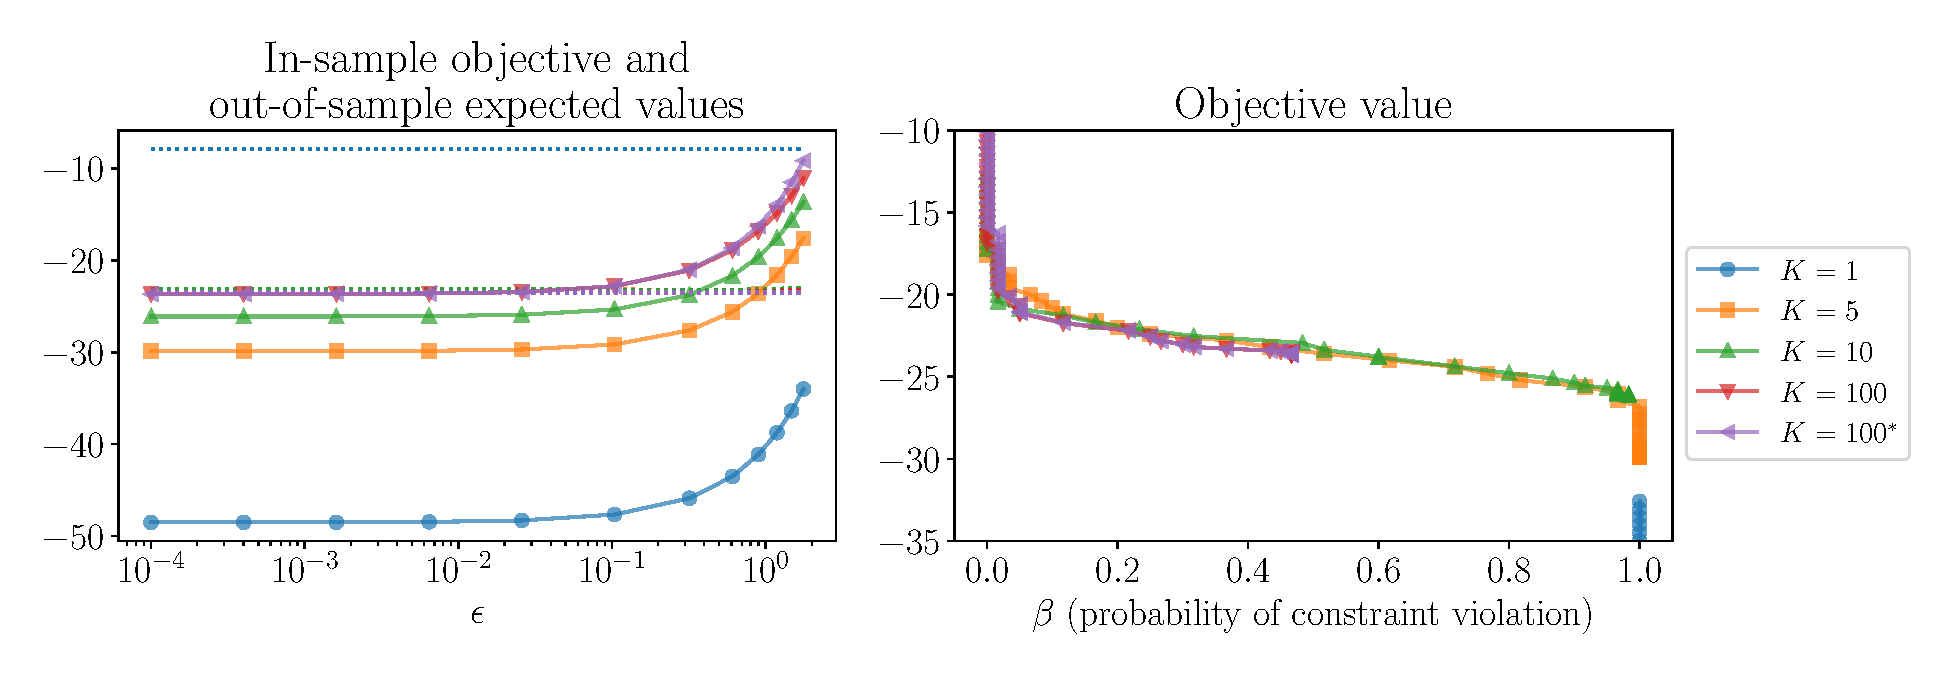
\includegraphics[width=\textwidth]{newstop.pdf}
	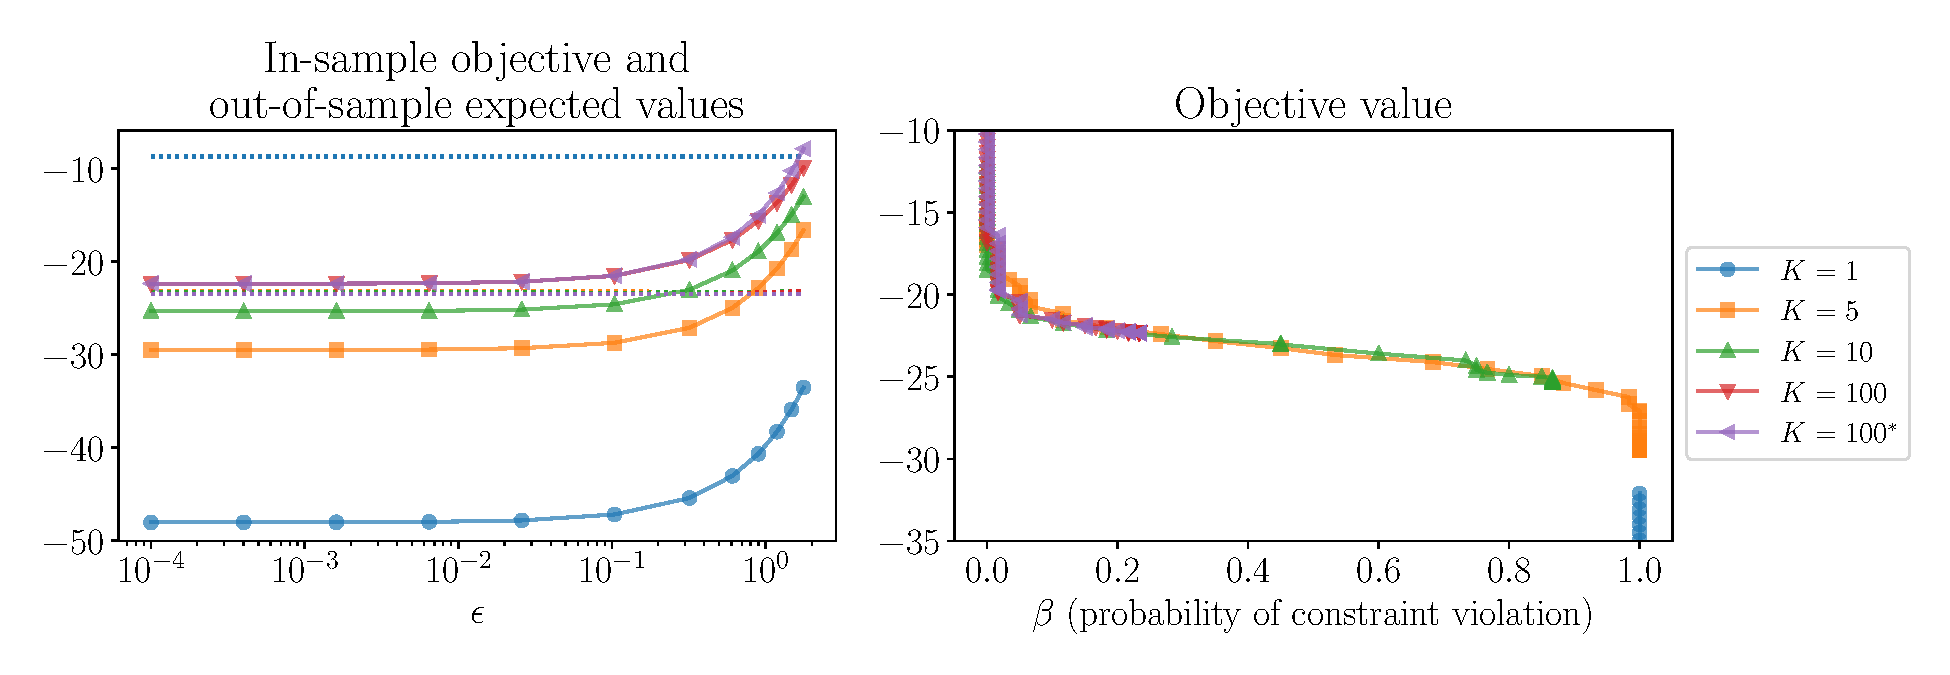
\includegraphics[width=\textwidth]{newstop_out.pdf}
	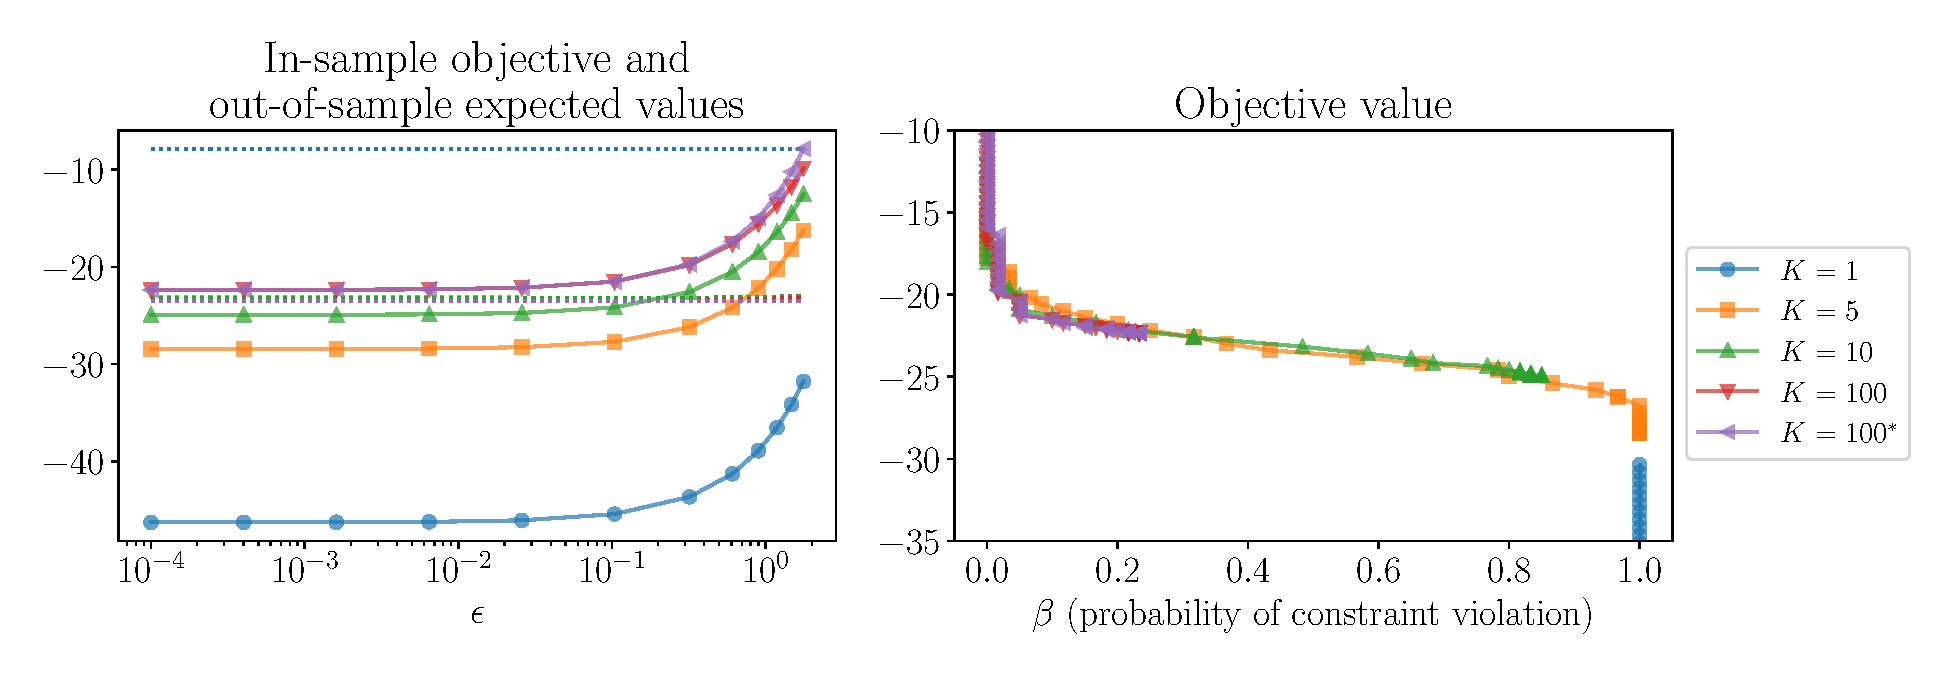
\includegraphics[width=\textwidth]{newstop_supp.pdf}
	\caption{Newsvendor. Left: in-sample objective values vs $\epsilon$ for different $K$. Right: objective value vs $\beta$ for different $K$; each point represents the solution for the $\epsilon$ achieving the smallest objective value.  $K = 100^*$ is the formulation without the support constraint. Top: \gls{MRO}. Middle: ROB-\gls{MRO}. Bottom: AUG-\gls{MRO}.}%
	\label{fig:news2}%
\end{figure}


\begin{figure}[h]%
	\centering
	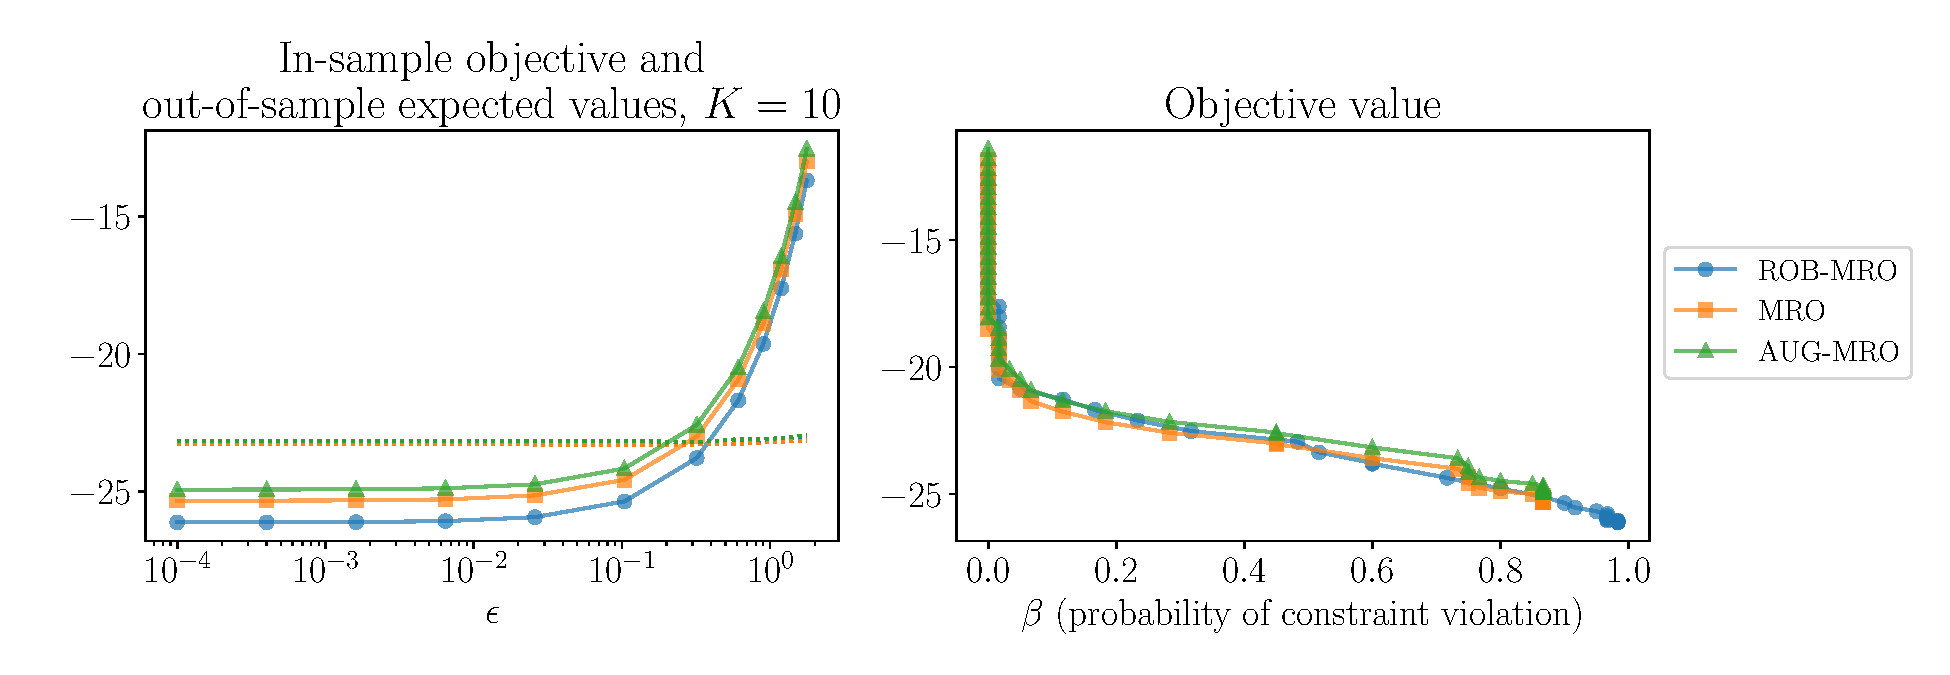
\includegraphics[width=\textwidth]{newscomp.pdf}
	\caption{Newsvendor. Left: in-sample objective values vs $\epsilon$ for  $K=10$. Right: objective value vs $\beta$ for $K=10$.}%
	\label{fig:newscomp}%
\end{figure}
\begin{figure}[h]%
	\centering
	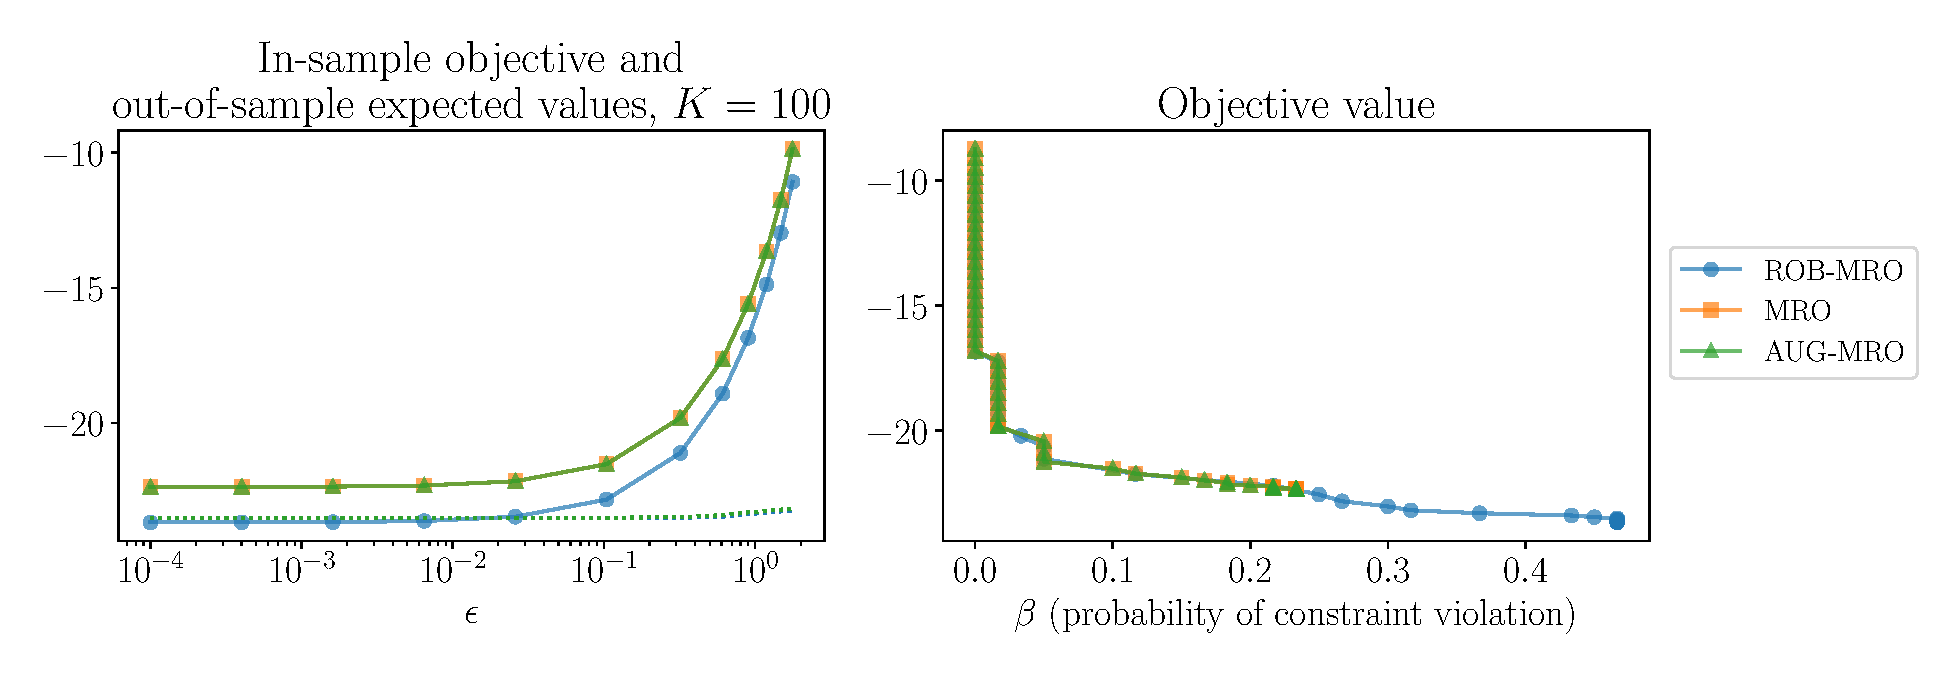
\includegraphics[width=\textwidth]{newscomp100.pdf}
	\caption{Newsvendor. Left: in-sample objective values vs $\epsilon$ for  $K=100$. Right: objective value vs $\beta$ for $K=100$.}%
	\label{fig:newscomp2}%
\end{figure}


\begin{figure}[h]%
	\centering
	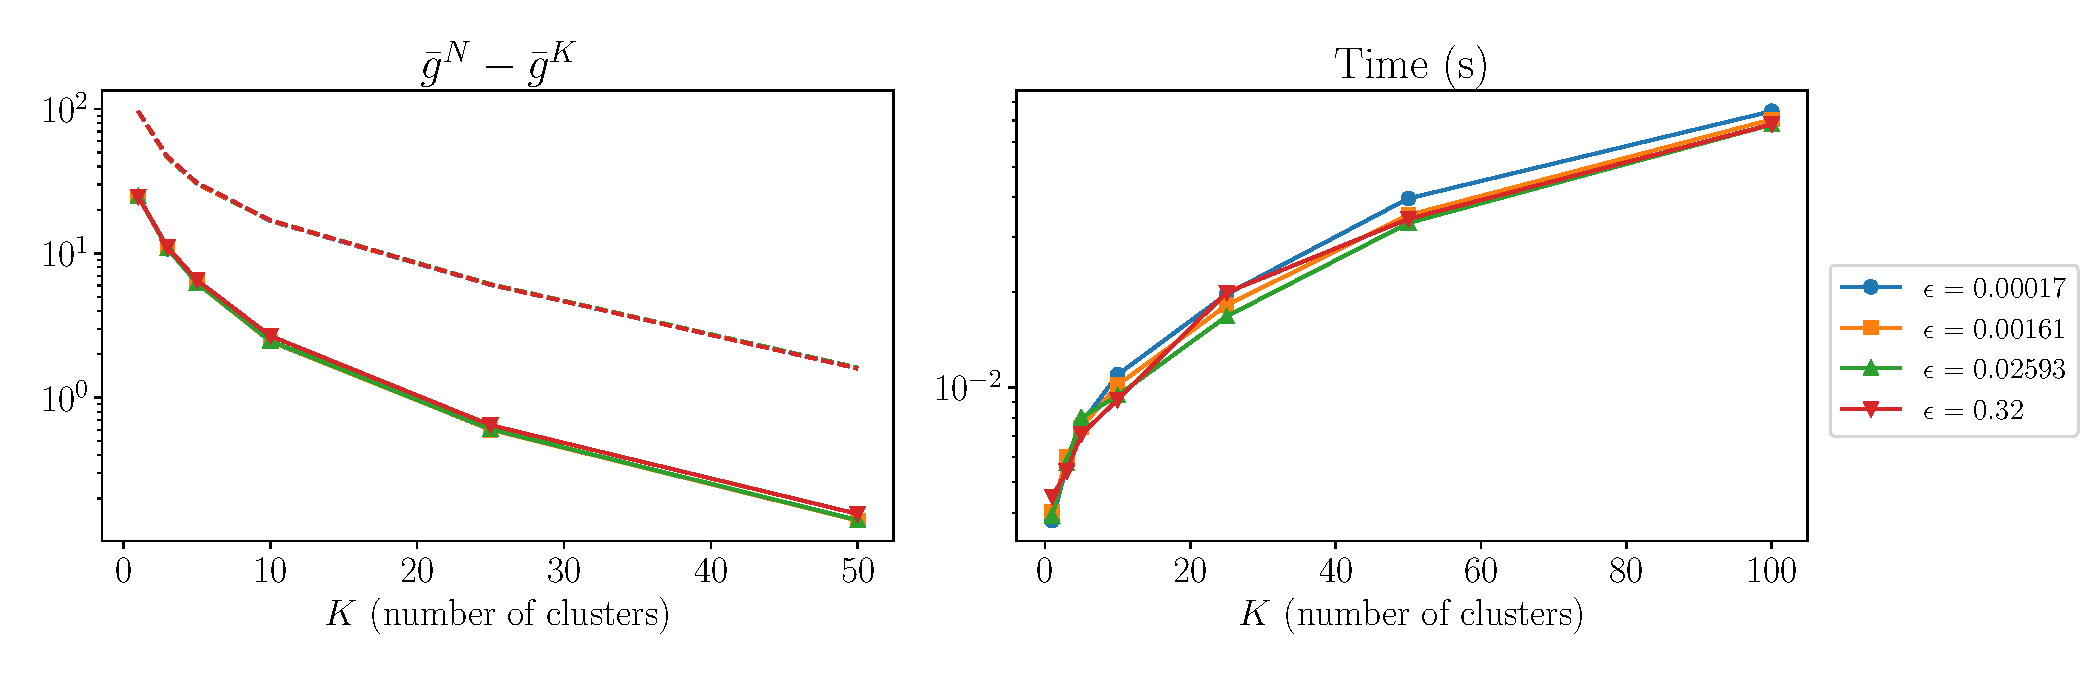
\includegraphics[width=\textwidth]{newsbot.pdf}
	\caption{Newsvendor. Left: the difference in the value of the uncertain objective between using $N$ and $K$ clusters, calculated as $\bar{g}^N(z) - \bar{g}^K(z)$, compared with the theoretical upper bound $\delta(K,y,\gamma)$ from Corollary~\ref{cor:maxaffine}. Solid lines are the difference, dotted lines are the upper bounds. Right: solve time. }%
	\label{fig:news3}%
\end{figure}


\chapter{Fast Online Distributionally Robust Optimization via Data Compression}
\label{chap:online_dro}

\glsresetall

\section{Introduction}
% This framework assumes the underlying probability distribution to be unknown, but lies in a known {\it ambiguity set} of probability distributions, from which the worst-case is taken. Such an approach is attractive in its ability to provide out-of-sample performance guarantees with a finite number of data-samples.
% By hedging against the ambiguity, it out-performs non-robust approaches such as~\gls{SAA}, with respect to worst-case performance. 

% Since its appearance, significant effort has been devoted to constructing ambiguity sets primarily in static settings, \RC{using either structural assumptions on the distribution (\eg, moments~\cite{moment,moment_1}) or training data directly~\cite{kuhn2019wasserstein,gao2016distributionally}.}
% % where a single set is used throughout; see~\cite{OPT-026,dro_survey,mohajerin2018data,gao2016distributionally}, and the references therein. 
% However, many real-time settings, such as healthcare resource allocation, air traffic control, and energy trading, are dynamic and new data becomes available sequentially over time.
% \RC{Despite its potential,~\gls{DRO} has been largely underdeveloped in such scenarios.
% Most~\gls{DRO} approaches construct a static ambiguity set, and model time progression through {\it adjustable wait-and-see variables}~\cite{adro2,adro,robustadaptopt}.}
% % Even in multi-stage~\gls{DRO}, where uncertain data is revealed sequentially, a single ambiguity set is typically constructed, with time progression modeled through {\it adjustable wait-and-see variables}~\cite{adro2,adro,robustadaptopt}. 
% % Fundamentally, this approach determines decisions based on {\it a priori} information.
% % Even in data-driven cases, the focus is on a fixed dataset from which the ambiguity set is constructed~\cite{}. 
% % However, in many real-time applications---such as healthcare resource allocation, air traffic control, and energy trading---new data becomes available sequentially over time. 
% % As a result, the optimizer's confidence in the nominal distribution can improve through the continuous assimilation of new data. 
% % More broadly, any application where an optimization problem is continuously re-solved for improved solutions can benefit from streaming data. %% Commented out after Marta's comment
% % into the ambiguity set.
% There are limited works focusing on how to adapt the ambiguity sets dynamically over time, where they pose strict assumptions on the problem: either by restricting the distribution to a finite set of scenarios~\cite{drotime}, or by requiring continuous variables and objective functions with local strong concavity~\cite{assim}.
% % In the few cases where it has been studied, updates to the~\gls{DRO} problem rely on gradient-based methods that either restrict the distribution to a finite set of scenarios~\cite{drotime}, or require continuous decision variables and objective functions with local strong concavity~\cite{assim}. 
% % To our knowledge, no online approach directly re-solves the \gls{DRO} problem as new data arrives, primarily due to the associated computational complexity.  % Commented out after Marta's comment
% % To our knowledge, there has not been online approaches where the \gls{DRO} problem is re-solved directly with the incorporation of streaming data, due to the increase in computational complexity. 
% \RC{In particular, streaming data settings can be challenging for the popular Wasserstein-based \gls{DRO}~\cite{mohajerin2018data,kuhn2019wasserstein,gao2016distributionally}, where the ambiguity set is defined as a Wasserstein ball around the empirical distribution of a dataset.}
% As new datapoints arrive, the problem dimension grows, increasing computational complexity~\cite{kuhn2019wasserstein,mro}.
% \RC{While a larger dataset improves confidence in the empirical measure as an approximation of the true distribution, the reduction in the ambiguity set’s radius is not enough to offset this complexity; for mixed-integer problems, even \gls{SAA} is difficult to solve with large amounts of data, without any added complexity from ambiguity. This leads to computational bottlenecks that are especially limiting for real-time applications.}
% % really don't like the word crippling


% , each increase in the sample size leads to an increase in the problem dimension. 
% Therefore, even though a larger number of datapoints leads to a higher confidence in the empirical measure as an approximation of the true distribution, the curse of dimensionality~\cite{gaoFiniteSampleGuaranteesWasserstein2023} dictates that the reduction in the ambiguity set radius is too slow to lead to a reduction in computational complexity, even with uncertain parameters of moderate dimensions. 
% In this work, we thus propose an online data compression approach to efficiently solve \gls{DRO} problems with streaming data, while ensuring guarantees on out-of-sample performance.
% the number of samples required before the~\gls{SAA} can be used as a reliable solution 


% Among the different settings proposed in recent years, we shall consider optimal transport-based \gls{acr:dro}, where the discrepancy between probability distributions is measured via an optimal transport distance.


% \bnote{Need to add story. An idea here
%     \begin{itemize}[noitemsep]
%     	\item DRO important, data-driven, but can be very expensive. Specifically with mixed-integer programs
% 	\item This is particularly true in streaming data settings where more and more samples arrive and increase the problem dimensions
% 	\item In this work, we propose a data compression approach to efficiently solve distributionally robust optimization problems with streaming data.
%     \end{itemize}
% }
% Here, $\epsnom_t > 0$ is a parameter that encapsulates our trust in the reference distribution.

% However, this comes at the expense of an increased computational burden as the reformulation of Problem \eqref{eq:DRO} is found to scale with the number of data $n_t$ employed in the construction of $\mathcal{P}_t$ \cite[Prop.~2.12]{shafieezadeh2023new}. 
% As a result, online \gls{DRO} with streaming data poses a fundamental \textit{dilemma} between statistics and computation. 
In this chapter, we extend the results of Chapter~\ref{chap:mro} to the online setting, where we consider access to streaming data. 
We formalize the problem-structure-dependent finite-sample probabilistic guarantees implied by the results of Section~\ref{sec:conservatism}, and further extend them to the asymptotic setting. 
For simplicity, we take the~\gls{DRO} view of the~\gls{MRO} problem, as noted in Section~\ref{sub:connectionsdro}, and restrict ourselves to an uncertain objective function $f$.

\subsection{Our contributions}%
\label{c3:sub:our_contributions}
% \bnote{briefly state how it overcomes the limitations that we just mentioned above}
We propose an {\rm online data compression approach} for efficiently solving Wasserstein~\gls{DRO} problems with streaming data, while also maintaining out-of-sample performance guarantees.
\RC{We allow for mixed-integer formulations, and a broad class of underlying distributions.}
Our key contributions are:
% \bnote{adjust abstract, conclusions, cover and nomination letters.}
\begin{itemize}
    % \item {\bf Online \gls{DRO} with data compression:} We develop an online algorithm that balances computational efficiency (through data compression) and solution quality. By adjusting the number of clusters, we trade off computational effort and performance adaptively. 
    % Online algorithm for DRO with streaming data, based on data-compression. Balance computational effort (number of clusters) and performance.
    \item {\it Adaptive ambiguity sets via online clustering:} We apply online clustering to construct {\it adaptive} ambiguity sets, formulated as Wasserstein balls of any order around a clustered empirical distribution.
    % adjusting a clustered empirical distribution over time to accurately capture the true underlying distribution. 
    We establish theoretical conditions on clustering algorithms to ensure the robustness of our framework, 
    which is compatible with any online clustering method that meets these conditions. 
    % Up to a finite time, the number of clusters and cluster assignments are allowed to shift freely, to accurately capture the underlying distribution.
    We relate to the concept of {\it optimal clustering},
     and provide  three  fast and memory-efficient  approximation algorithms suitable for our purposes. 
    
    \item {\it Clustering effect analysis:}  
    % \item {\bf Finite-sample and asymptotic guarantees:} 
    % We provide certificates, \ie, upper bounds on the out-of-sample performance of our algorithm, and
    \RC{We prove that the performance gap between our compressed solution and the non-compressed (nominal) \gls{DRO} solution can be written in terms of the discrepancy between the true distribution and its clustered approximation, together with the ambiguity set radius. Under mild assumptions, this radius can decay at a rate independent of the uncertainty dimension.}~We also show that our objective converges to a value dependent on the number of clusters and the quality of the clustering algorithm. 
    This quantifies the impact of data compression, and highlights the {\it trade-off between computational effort and optimality.}
    \RC{We provide both finite-sample and asymptotic performance guarantees for our solution.}
    % and establishes the number of clusters as an adjustable parameter. 
    % by adjusting the number of clusters, we trade off computational effort and 
% \ifpreprint
    \item {\it Online regret analysis:} 
    % \item {\bf Regret analysis:} 
    We provide a regret analysis comparing the performance of our algorithm to the one of non-compressed \gls{DRO} {\it in hindsight}, \ie, with access to the subsequent realization of the uncertainty. 
    We show that the regret converges sublinearly to a function of the Wasserstein distance between the true and compressed distributions, and with probability 1, the difference induced by the time-discrepancy converges to 0.
%     % : 
%     % ensuring that our online approach successfully approximates the non-compressed \gls{DRO} solution.
% \fi
    \item {\it Computational gains in numerical experiments:} We demonstrate the efficiency of our approach in sparse portfolio optimization. Our results show significant computational savings, even compared to~\gls{SAA}, with minimal loss in solution quality.
    We also demonstrate the possibility for the online framework to be memory-efficient, allowing the optimizer to discard datapoints once seen, with minimal impact on solution times and quality.  

\end{itemize}

% \bnote{still need to complete this}
% \begin{itemize}
% \item fast and memory efficient online clustering algorithm for distributionally robust optimization.
% \item performance guarantees, finite-sample and asymptotic, for both bounded and unbounded support. We give both upper and lower bounds, and show convergence of the online solutions to some clustering-dependent value, at the same rate of convergence as nominal \gls{DRO}.
% These work with any clustering algorithm satisfying mild assumptions, and for any computational budget $K$.
% \item the number of clusters do not need to be constant throughout the algorithm for the finite sample results. For the asymptotic results, we only require the number of cluster and cluster supports to be constant after some finite time $\tau$
% \item dynamic regret bounds where we assume information latency
% \item works for mixed-integer optimization problems
% \item numerical experiments where we demonstrate computational speedups
% \end{itemize}

% \bnote{I would try to highlight the contributions without introducing too many math symbols yet since we haven't defined anything so far. I brought some of this to the contributions already}
% For each of the online decisions, dependent on the adaptive radius $\eps_t$, we obtain finite sample performance guarantees similar to~\eqref{c3:eq:prob_guarantees1}, as well as asymptotic guarantees as $t \to \infty$.
% Specifically, we show the relationship between the performance of our online decision, the optimal \gls{DRO} solution, as well as the true optimal solution, and note that the gap in performance converges to a function of the data-compression loss: the distance $W_p(\prob,\prob^K_\star)$ between the true distribution $\prob$ and a converged data-compressed distribution $\prob^K_\star$.

% We show that with probability $1$, the regret again converges to a function of $W_p(\prob,\prob^K_\star)$, and the convergence to this value is sublinear in $T$. The sublinear convergence certifies that the considered online algorithm successfully approximates the \gls{DRO} solution with an average gap that decreases over time.

% \subsection{Related work}%
% \label{c3:sub:related_work}

% \bnote{The selection committee is Jim Luedtke (University of Wisconsin-Madison, chair), Milo\v{s} Kopa (Charles University in Prague), and Karmel S. Shehadeh (Lehigh University). Let's make sure we cite their papers. The first and last one especially have several papers on stochastic programming/DRO/etc}

% \paragraph{Online saddle-point tracking.}


% In this work, we adapt two algorithms for our purposes. 
% Specifically, CluStream works in two phases: an online phase where it maintains a set of micro-clusters (i.e., summary statistics of the observed data), and and offline phase that periodically applies traditional clustering methods on the micro-clusters to generate macro-clusters. \MartaNote{Comment on the differences w.r.t. our version? Is it going to be cut?}

% \bnote{change layout}
\subsection{Layout of the chapter}
The rest of this chapter is organized as follows.
In Section~\ref{sec:problem_intro}, we state the problem and introduce our online algorithm, and in Section~\ref{sec:general_intro}, analyze the clustering effect by providing finite sample and asymptotic performance guarantees.
% , for distributions satisfying light-tailed assumptions, and with arbitrary online clustering algorithms satisfying mild requirements. 
% in Section~\ref{sec:bounded_perf}, we examine the special case of bounded support.
% , and give alternative performance guarantees. 
In Section~\ref{sec:bounded_perf}, we give theoretical results for the specific case of bounded support. 
In Section~\ref{sec:regret}, we introduce the notion of dynamic regret and give corresponding bounds.
In Section~\ref{sec:algos}, we describe various online clustering algorithms, and
% with different runtime and space complexities.
in Section~\ref{sec:hyper_param}, give guidelines for choosing the number of clusters and the ambiguity set radii experimentally. In Section~\ref{sec:exampless} we demonstrate our results on a portfolio optimization example. 
% We summarize our conclusions in Section~\ref{c3:sec:conclusions}.

\section{The online stochastic problem}
\label{sec:problem_intro}
% \RC{In this section, we introduce our problem setting and standing assumptions. For conciseness, these assumptions will not be explicitly imposed in subsequent theorems.}
Following the notation and general setting of Chapter~\ref{chap:prelim}, we consider a \gls{SO} problem of the form
\begin{equation}
\label{eq:opt}
 H_\star  = \min_{z\in \mathcal{Z}} \mathbf{E}_{\unc \sim \mathbf{P}}[f(\unc,z)],
\end{equation}
where $z \in \mathcal{Z} \subseteq \reals^n$ is the decision variable, $\unc \in \supp \subseteq \reals^m$ the vector of uncertain parameters governed by $\prob$, and $H_\star$ the optimal objective value.
The assumptions on the support and domain of $f$ follow exactly from Chapter~\ref{chap:mro}.
%  and we assume that Assumption~\ref{assp:dom} on the $\dom{f}$ holds throughout the chapter. 
% We assume that the support $\supp$ of $\prob$ lives within the domain of $f$ for the variable $u$, which we will refer to as $\dom{f}$, \ie, $\supp \subseteq \dom{f}$.
The function $f:\mathcal{Z}\times \supp \rightarrow (-\infty, \infty]$ is again assumed to be of the maximum-of-concave form satisfying Assumption~\ref{ass:convex_l}, \ie,
$f(u, z) = \max_{j\leq J}f_j(u,z),$
with each $f_j$ being proper, concave, and upper-semicontinuous in~$u$ for all $z$.
Additionally, we require the functions $f_j$ to be either Lipschitz or smooth for all $z \in \mathcal{Z}$, according to the following definitions. We assume the existence of the global constants independent of $z$ by the compactness of $\mathcal{Z}$.
% \bnote{Should this result hold for any $x$? Otherwise, we would need $M_x$.}
% \begin{definition}[Lipschitzness]
% 	\label{def:lip}
% 	A function $f(u,x)$ is $M$-Lipschitz on its domain with respect to the $\ell_2$-norm, if for all $x \in \mathcal{X}$,
%     \vspace{-0.6em}
% 	\begin{equation*}
% 	\textstyle	\left |f(v,x) - f(u,x)\right| \leq M\| u - v\|_2, \quad \forall u,v \in \dom f.
% 	\end{equation*}
%  %    In addition, it is $L^{(2)}$-Lipschitz on its domain, with constant $L^{(2)}$, with respect to the $\ell_2$-norm and for a given $u$, if 
% 	% \begin{equation*}
% 	% \textstyle	\left |f(u,x) - f(u,x')\right| \leq L^{(2)}\| x - x'\|_2, \quad \forall x,x' \in \mathcal{X}.
% 	% \end{equation*}
% \end{definition}
% \begin{definition}[Smoothness]
% 	\label{def:smooth}
% 	A differentiable function $f(u,x)$ is $L$-smooth on its domain, with respect to the $\ell_2$-norm, if for all $x \in \mathcal{X}$, 
%     \vspace{-0.6em}
% 	\begin{equation*}
% 	\textstyle	\left\|\nabla f(v,x) - \nabla f(u,x)\right\|_2 \leq L\| u - v\|_2, \quad \forall u,v \in \dom f.
% 	\end{equation*}
% \end{definition}
\begin{assumption}[Lipschitzness and smoothness]
\label{ass:general_ass_lip} \RC{Let at least one hold.
    \begin{enumerate}
        \item For all $z \in \mathcal{Z}$, the constituent functions $f_j$ of $f$ are Lipschitz continuous with constants~$M_j$, \ie, $\left |f_j(v,z) - f_j(u,z)\right| \leq M_j\| u - v\|_2, \; \forall u,v \in \dom f$.
        \item For all $z \in \mathcal{Z}$, the constituent functions $f_j$ of $f$ are smooth with constants~$L_j$, \ie, $\left\|\nabla f_j(v,z) - \nabla f_j(u,z)\right\|_2 \leq L_j\| u - v\|_2,\; \forall u,v \in \dom f$.
        \item For all $z \in \mathcal{Z}$, $f$ is smooth with constant ~$L$, \ie, $\left\|\nabla f(v,z) - \nabla f(u,z)\right\|_2 \leq L\| u - v\|_2,\; \forall u,v \in \dom f$.
    \end{enumerate}}
\end{assumption}
% \RC{Note that if clause 3 is satisfied and $f$ is concave, clause 2 is also satisfied with $J = 1$.}

% $\dom{f}$ to be independent of $x$, and satisfies the following.
% We assume $f$ is either element-wise monotonically increasing in $u$ and only has a (potentially) lower-bounded domain, or element-wise monotonically decreasing in $u$ and only has a (potentially) upper-bounded domain.
% Otherwise, we assume $\dom{f}$ is $\reals^m$.}
% \begin{assumption}
% 	\label{assp:dom}
% 	The domain $\dom{f}$ is $\reals^m$. Otherwise, $f$ is either element-wise monotonically increasing in $u$ and only has a (potentially) lower-bounded domain, or element-wise monotonically decreasing in $u$ and only has a (potentially) upper-bounded domain. In all cases, the domain $\dom{f}$ is independent of $x$.
% \end{assumption}

% Despite that stochastic optimization problems are ubiquitous in many research areas \cite{shapiro2021lectures}, their practical deployment 
% is hindered by a fundamental
% challenge, namely that the distribution $\mathbf{P}$ governing $\unc$ is rarely accessible to the decision maker. 
% \bnote{the phrase before is good but more suited for the intro. I would just start with ``we assume $\prob$ to be ..., and only accessible through streaming data...''}


% Analogously to~\cite{mro}, we make the following assumptions on $\prob$, that commonly apply in practice.

\paragraph{Streaming data}
We assume the distribution $\prob$ to be unknown, and that the value $H_\star$ cannot be calculated as is. 
However, we have access to a {\it streaming dataset} of i.i.d.\ realization of $u$, which we use to construct an uncertainty framework. 
We begin with an initial dataset with $n_0 \geq 1$ datapoints, \ie, $\mathcal{D}_0 = \{\hat{u}^i\}_{i=1}^{n_0}$. Then, at the end of each time step $t \geq 1$, the dataset is updated to be $\mathcal{D}_t = \{\hat{\unc}^{i}\}_{i=1}^{n_0 + t}$, with $|\mathcal{D}_t| = n_t = n_0 + t$. That is, we assume w.l.o.g. that one realization gets disclosed at the end of each time step. Furthermore, we define the empirical distribution $\hat{\prob}_t = (1/{n_t})\sum_{i=1}^{n_t} \delta_{\hat{\unc}^{i}},$
where $\delta_u$ is the Dirac distribution concentrating unit mass on $u$, and $\prob^t$ the product distribution of the dataset. 



% \RC{We denote by $r$ the specific order chosen for the Wasserstein ambiguity set.}
% \bnote{mention what $\delta$ is}
% \IrinaNote{done}

\subsection{\Gls{DRO} over time}
\label{sec:over_time}
% Using the Wasserstein distance $W_p$ defined in Chapter~\ref{chap:prelim} (see~\eqref{eq:wass_dist}), let $\Xi_{\barp}(S)$ be the space of all probability distributions $\mathbf{Q}$ defined on the support~$\supp$, with bounded $\barp$-th moments, \ie,
% $\Expect_\mathbf{Q}[\|u\|^{\barp}] = \int_S\|u\|^{\barp}\mathbf{Q}(du) < \infty$, where $\|\cdot\|$ is an arbitrary norm on $\reals^m$, \RC{and either $\barp\geq 1$ or $\barp = \infty$.
% }
In this work, to differentiate from the analysis on general Wasserstein-$p$ distances in Section~\ref{sec:cluster_prop}, we always refer to $r$ as the order of the Wasserstein distance used within an ambiguity set.
As introduced in Section~\ref{sec:dro_def}, at each time $t$, the~\gls{DRO} approach under the Wasserstein metric constructs an ambiguity set \RC{of order $r$} around $\hat{\prob}_t$ of radius $\epsnom_t \geq 0$, \ie,
\begin{equation}\label{empirical:ball}
\mathcal{P}_t = \mathbf{B}_{\epsnom_t}^r(\hat{\prob}_t)=\left\{\mathbf{Q} \in \mathcal{M}_{r}({\supp}) \mid W_r(\hat{\prob}_t, \mathbf{Q}) \leq \epsnom_t\right\},
\end{equation}
% \RC{In this work, we always refer to $r$ as the order of the Wasserstein distance used within an ambiguity set. For other Wasserstein distances used in the analysis, we refer to order $p$.
% In addition, whenever we use a distance metric of order~$p$ on a distribution $\mathbf{Q}$, we assume that the distribution itself has finite~$\barp$-th moments.}
% \RC{We suppress the dependency of $\mathcal{P}_t$ on $r$ for conciseness, and note that unless otherwise specified, $r$ is of an arbitrary order and $\|\cdot\|$ is an arbitrary norm.}
and the~\gls{DRO} solution $z_t \in \mathcal{Z}$ is computed by solving the optimization problem
\begin{equation}\label{eq:DRO}
H_t = \min_{z \in \mathcal{Z}} \max_{\mathbf{Q} \in \mathcal{P}_{t}}\mathbf{E}_{\unc \sim \mathbf{Q}}[f(\unc,z)].
\end{equation}
% where we seek to minimize the worst-case (w.r.t.\ \textit{any} distribution in the ambiguity set) expected value of $f$. 
% Note that we use the ambiguity set $\mathcal{P}_{t-1}$ constructed at time $t-1$: in the online framework, we assume to solve the problem {\it before} the new datapoint is revealed. 
\label{subsec:nom_perf}
As~$t$ increases, our confidence in $\hat{\prob}_t$ increases, allowing us to safely reduce the radius~$\epsnom_t$, which can be interpreted as a measure of trust in the data.
\RC{With suitable choices of $\epsnom_t$ (given in Theorems~\ref{thm:measure_gen},~\ref{theorem-inf},~\ref{thm:informal_curse}), which we from here on refer to as the {\it nominal radius}, we obtain
{\it finite sample performance guarantees} of the form}
\begin{equation}
	\label{c3:eq:prob_guarantees1}
	\RC{\prob^{t}\left( H_\star \leq \mathbf{E}_{\prob}[f(u, z_t)] \le H_t + \rho_{t}\right) \ge 1 - \beta_{t},}
\end{equation}
where for all $t\geq 1$, $\beta_{t} > 0$ is a specified time-varying
probability of constraint violation, and $\rho_{t}$ is a residual term.
Following the results of Section~\ref{sec:dro_def}, for $\epsilon_t$ chosen from Theorems~\ref{thm:measure_gen} and~\ref{theorem-inf}, $\rho_t = 0$, and for $\epsilon_t$ chosen from Theorem~\ref{thm:informal_curse}, $\rho_t = \tilde{O}(n_t^{-1/2})$.

As noted in the previous chapters, while powerful, such a formulation is susceptible to prohibitive solution times as $N$ grows. This leads to computational bottlenecks that are especially limiting for real-time applications. We thus adapt our~\gls{MRO} approach from Chapter~\ref{chap:mro} to this real-time setting, which enjoys cost-savings in every iteration. 
% \RC{Specifically, under mild assumptions, choosing $\epsnom_t \sim \text{o}(t^{-\frac{1}{d}})$ ensures that the true distribution $\mathbf{P} \in \mathcal{P}_t$ with high probability, which gives the above guarantee with $\rho_{t-1} = 0$~\cite{fournier2015rate,mohajerin2018data}.}  
% The in-sample objective value $H_t$ is then a {\it certificate} for the out-of-sample performance $\Expect_{\prob}[f(u, x_t)]$.
% \RC{In this work, we make use of two such choices of $\epsnom_t$, which require the distribution $\prob$ to satisfy distinct assumptions. We summarize them here.}

% \paragraph{Dimension-dependent} \RC{One choice is to impose a light-tailed assumption, which is satisfied by sub-Gaussian distributions and by bounded distributions.}
% % \begin{assumption}[Light-tailed distribution]
% % \label{ass:light_tail}
% %     There exists an exponent \RC{$\alpha > 1$, such that
% %     $R = \Expect_\prob[\exp(\|u\|^{\alpha})] = \int_S \exp(\|u\|^{\alpha})\prob(du) < \infty.$}
% % \end{assumption}
% \RC{Then, measure concentration results for Wasserstein-$\barp$ distances imply the following.}
% % \RC{Satisfaction of this assumption for the case $\barp \geq 1$, and the satisfaction of analogous but stronger assumptions for the case $\barp = \infty$~\cite{wass-p-guarantee}, gives the following guarantee:}
% % \begin{theorem}[Measure concentration, light-tailed~\cite{fournier2015rate}]
% % \label{thm:measure_gen}
% % \RC{Let $\barp \geq 1$. If Assumption~\ref{ass:light_tail} holds with $r > \barp$ for the distribution $\prob$ and empirical distribution $\hat{\prob}^N$ supported on $N$ points, we have
% %   $$  \mathbf{P}^N(W_{\barp}(\mathbf{P},\hat{\mathbf{P}}^N) \geq \epsnom)
% %   \leq \begin{cases}
% %     c_1 \exp(-c_2N \epsnom^{\max\{d/{\barp},2\}}) \quad \textit{if } \epsnom \leq 1\\
% %     c_1 \exp(-c_2N \epsnom^{r/{\barp}}) \quad \textit{if }  \epsnom > 1,
% %   \end{cases}$$
% %   for all $\epsnom >0$, $m \neq 2{\barp}$, and $N \geq 1$. If Assumption~\ref{ass:light_tail} holds with $r \in (1,\barp)$, we have
% %     $$  \mathbf{P}^N(W_{\barp}(\mathbf{P},\hat{\mathbf{P}}^N) \geq \epsnom)
% %   \leq \begin{cases}
% %     c_1 \exp(-c_2N \epsnom^{\max\{d,2{\barp}\}}) + \exp(-c_2 (N\epsnom^{\barp})^\frac{r-s}{\barp})  \\
% %     \hfill \textit{if } \epsnom \leq 1, \forall s \in (0,r)\\
% %     c_1 \exp(-c_2 (N \epsnom^{\barp})^{r/{\barp}}) \quad \textit{if }  \epsnom > 1,
% %   \end{cases}$$
% % for all $\epsnom > 0$, $m \neq 2\barp$, and $N \geq 1$. For all cases, $c_1,c_2$ are positive constants depending only on $R,r,s,$ and $d$.}
% % \end{theorem}
% % For the special case $\barp = \infty$, we point to~\cite[Theorem 1.1]{wass-p-guarantee} for an analogous result, which assumes a stronger condition than Assumption~\ref{ass:light_tail}.
% % Using these relations, the radius for a Wasserstein~\gls{DRO} ambiguity set with $N = n_{t-1}$ points \RC{and order $\barp = p$} can be chosen by setting the right-hand-side to $\beta_{t-1}$, then solving for $\epsnom_{t-1}$. See~\cite[Theorem 3.4]{mohajerin2018data} for the case $\barp=1$. The procedure for $\barp > 1$ follow similarly. \RC{We summarize them as follows.} 
% \begin{theorem}[Guarantees using Wasserstein measure concentration~\cite{fournier2015rate,kuhn2019wasserstein}]
%     \label{thm:calc_eps}
%     \RC{Let $\barp$ be an arbitrary order. 
%     Under Assumption~\ref{ass:light_tail} for the case $\barp \geq 1$, and under analogous assumptions for $\barp =\infty$~\cite{wass-p-guarantee}, for $n_t \rightarrow \infty$ we can choose confidence levels $\beta_t \in (0,1)$ and corresponding radii $\epsnom_t=O((\log(\beta^{-1}_t)/{n_t})^{\min(\barp/m,1/2)})$ such that $\sum_{t=1}^\infty \beta_t < \infty$,
%     $\prob^{t}(W_{\barp}(\prob,\hat{\prob}_t) \geq \epsnom_t) \leq \beta_t,$ and $\lim_{t \rightarrow \infty} \epsnom_t = 0.$ The~\gls{DRO} problem~\eqref{eq:DRO} solved with $r = \barp$ and these radii gives the finite-sample guarantee~\eqref{c3:eq:prob_guarantees1} with $\rho_{t} = 0$.}
%     % $$\prob^{t-1}\left( H_\star \leq \Expect_{\prob}[f(u, x_t)] \le H_t\right) \ge 1 - \beta_{t-1}.$$
% \end{theorem}
% % In all cases, we note that the radius is inversely related to the number of datapoints, \ie, the larger the number $n_t$, the smaller $\epsnom_t$ can be. 
% % With the radius chosen in this way, we obtain the~\gls{DRO} performance guarantees~\eqref{c3:eq:prob_guarantees1} using~\cite[Theorem 3.5]{mohajerin2018data}.

% % \begin{theorem}[Nominal \gls{DRO} guarantee]
% % \label{thm:dro_nom}
% % The solution $x_t$ and optimal value $H_t$ of the \gls{DRO} problem with radius $\epsnom_{t-1}$ implies the finite sample performance guarantee 
% % \begin{equation*}
% % 	\prob^{n_{t-1}}\left( H_\star \leq \Expect_{\prob}[f(u, x_t)] \le H_t \right) \ge 1 - \beta_{t-1}.
% % \end{equation*}
% % \end{theorem}
% \RC{We point to the cited works~\cite{fournier2015rate,wass-p-guarantee,kuhn2019wasserstein} for the constants involved.}

% In Section~\ref{sec:bounded_perf}, we further calculate explicit radii for the specific case of bounded support $\supp$. 

% From the above characterization, it is evident that larger datasets are beneficial for reducing the distributional ambiguity around the nominal distribution. 
% Indeed, we can \RC{use Theorem~\ref{thm:calc_eps}} to conclude that $\mathbf{P}^\infty \{ \lim_{t \rightarrow \infty} W_r(\mathbf{P}, \hat{\mathbf{P}}_t)\RC{ =0} \} = 1$, which implies \RC{$\mathbf{P}^\infty \{\lim_{t \rightarrow \infty}H_t \downarrow H_\star\}=1$ under the Lipschitz condition of Assumption~\ref{ass:general_ass_lip}~\cite[Theorem 3.7]{mohajerin2018data}.} \RC{However, as the radius scales with $O(n_t^{-r/m})$, even for moderately sized $m$ this bound suffers from the curse of dimensionality.}
% \RC{The slow decrease in the required radius while the dataset grows} makes the resolution of the \gls{DRO} problem in \eqref{eq:DRO} computationally challenging, as a constraint needs to be added for each datapoint constituting the empirical distribution  $\hat{\mathbf{P}}_t$ (see formulation~\eqref{c3:eq:robustopt_p_max}). 
% Clearly, for $t \rightarrow \infty$, we would end up with an infinite-dimensional problem that cannot be solved. 

% \paragraph{Dimension-free} 
% \RC{Recent work~\cite{gao2016distributionally} decouples the radii $\epsnom_t$ from the dimension $m$ by providing finite sample guarantees for type-$r$ Wasserstein~\gls{DRO}, $r \in [1,2]$, with radii scaling as $\tilde{O}(n_t^{-1/2})$~($\tilde{O}$ suppresses logarithmic terms). %, breaking the curse of dimensionality. 
% These result require $\prob$ to satisfy a transportation-information inequality, and $f$ to satisfy certain curvature conditions, stated below for completeness.
% \begin{assumption}
% \label{ass:gao}
%     If we consider $r= 1$ for~\eqref{empirical:ball}, then $\prob$ satisfies the transportation-information inequality $T_1(\alpha)$ for some positive constant $\alpha$, \ie, for all $\mathbf{Q}\in \Xi_1(\supp)$, $W_1(\mathbf{Q},\prob) \leq \sqrt{\alpha H(\mathbf{Q}\|\prob)}$, where $H(\mathbf{Q}\|\prob)$ denotes the relative entropy. Furthermore, $f$ satisfies clause 1 of Assumption~\ref{ass:general_ass_lip}. If $r=2$, then $\prob$ satisfies $T_2(\alpha)$ for some positive constant $\alpha$, and $f$ satisfies clause 3 of Assumption~\ref{ass:general_ass_lip}.
% \end{assumption} If the objective function class $\mathcal{F}=\{f(\cdot,x)\mid x\in\mathcal{X}\}$ additionally satisfies certain assumptions on its Rademacher complexity~\cite[Assumption 5]{gao2016distributionally}, the following holds.}
% \RC{\begin{theorem}[Dimension-free performance guarantees~\cite{gao2016distributionally}]
% \label{thm:informal_curse} 
% For orders $r =1$ and $r=2$, under Assumption~\ref{ass:gao} and a Rademacher complexity condition~\cite[Assumption 5]{gao2016distributionally}, we can choose confidence levels $\beta_t \in (0,1)$, radii $\epsnom_t=\tilde{O}(n_t^{-1/2})$, and residual terms $\rho_{t} = \tilde{O}(1/n_t)$ such that for all $x \in \mathcal{X}$, 
% \begin{equation}
% 	\label{eq:informal_x}
% 	\prob^{t}\left(\Expect_{\prob}[f(u, x)] \le  \max_{\mathbf{Q} \in \mathcal{P}_{t}}\mathbf{E}_{ \mathbf{Q}}[f(\unc,x)]+ \rho_{t}\right) \ge 1 - \beta_{t}.
% \end{equation}
% This implies the finite-sample guarantee~\eqref{c3:eq:prob_guarantees1} with the above parameter values.
%     % $$\prob^{t-1}\left( H_\star \leq \Expect_{\prob}[f(u, x_t)] \le H_t+\rho_{t-1}\right) \ge 1 - \beta_{t-1}.$$
% \end{theorem}}
% \RC{In exchange for dimension-free radii $\epsnom_t$, this result introduces a nonzero residual~$\rho_t$. However, even with smaller radii, the difficulty of solving the DRO problem with a large number of datapoints can be high. We are thus motivated to introduce an additional tradeoff, where a separate residual term is established in exchange for a more compact \gls{DRO} formulation. This leads to our framework below. }




 % Mohajerin Esfahani and Kuhn~\cite{mohajerin2018data} prove that appropriately decreasing choices of $\epsnom_t$ and $\beta_t$ as $t \to \infty$ also lead to {\it asymptotic} guarantees on the convergence of $H_t$ to the true value $H_\star$. 
 % These results imply, by incorporating streaming data into~\eqref{eq:DRO}, we can \textit{adapt} the ambiguity set and gradually reduce the cost of robustness. 

\subsection{Our online algorithm}
\label{subsec:ours}
% While incorporating streaming data improves the solution quality, it also increases the computational burden.
% scaling with the number of datapoints~\cite{mohajerin2018data}.
%(See also~\eqref{c3:eq:robustopt_p_max} below\bnote{I would remove citation to future parts}). 
We propose a data-compression framework for fast online \gls{DRO}. 
Our goal is to solve an adjusted \gls{DRO} problem over time, \RC{where $K$ is the chosen number of data clusters, and}
\begin{equation}\label{eq:dro:time}
H^K_t = \min_{z \in \mathcal{Z}} \max_{\mathbf{Q} \in \mathcal{P}^K_{t}}\mathbf{E}_{\unc \sim \mathbf{Q}}[f(\unc,z)],\quad t=1,2,\dots
\end{equation}
with $\mathcal{P}^K_{t}$ an {\it adaptive ambiguity set}, with adaptive radius $\eps_{t} \geq 0$, constructed from the data $\mathcal{D}_{t}$ observed so far. 
From here onward, we refer to the solution $z^K_t$ as the {\it online} solution, and the solution $z_t$ from~\eqref{eq:DRO} as the {\it nominal}~\gls{DRO} solution.
\begin{definition}[Adaptive ambiguity set]
The adaptive ambiguity set at the end of time period $t$, with radius $\eps_{t}\geq0$ and reference distribution $\hat{\mathbf{P}}^K_{t}$, is given by
\begin{equation}\label{empirical:ball_t}
\mathcal{P}^K_t = \mathbf{B}_{\eps_{t}}^r(\hat{\mathbf{P}}^K_{t})=\left\{\mathbf{Q} \in \mathcal{M}_r({\supp}) \mid W_r(\hat{\mathbf{P}}^K_{t}, \mathbf{Q}) \leq \eps_{t}\right\}.
\end{equation}
\end{definition}
Unlike the standard \gls{DRO} ambiguity set, the adaptive ambiguity set is {\it compressed} in that we allow the reference distribution to be supported on only $K \leq n_t$ points.
% , to greatly reduce the computational burden. 
With access to the dataset $\mathcal{D}_t$, the reference distribution is formulated by {\it clustering} the datapoints into sets $C^k_t$, $k = 1, \dots,K_t,$ where $K_t \leq K$.
% consisting of cluster weights $\theta^k_t$ and cluster centroids $\bar{\unc}^k_t$. 
The weight $\theta^k_t$ of a cluster $C^k_t$ is defined as the proportion of total points in the cluster, and the cluster \RC{mean}~$\bar{\unc}^k_t$ is the mean of these points. These values characterize the clustered empirical distribution~$\hat{\prob}^K_t$,~\ie,
$$\theta_t^k = \frac{n^k_t}{n_t},\quad \bar{u}^k_t = \frac{1}{n^t_k} \sum_{\hat{u} \in C^k_t} \hat{u},\quad \hat{\mathbf{P}}^K_t = \sum_{k=1}^{K_t}\theta_t^k\delta_{\bar{u}_t^k},$$ 
where $n^k_t = |C^k_t|$.
In Section~\ref{sec:shared_cluster}, we provide additional details on our clustering requirements, and in Section~\ref{sec:algos}, provide efficient online clustering methods. 

With an adaptive ambiguity set $\mathcal{P}^K_{t}$, we solve the online compressed~\gls{DRO} problem~\eqref{eq:dro:time} through a direct reformulation approach (as introduced in Section~\ref{sec:max_concave}), given as
\begin{equation}
	 \label{c3:eq:robustopt_p_max}
	\begin{array}{lll}
 \!\!H^K_t \!= \!\!\!&\underset{z\in\mathcal{Z},\lambda_t\geq0,s_t,y_t,h_t}{\mbox{minimize}} & \sum_{k=1}^{K_t} \theta^k_{t} s^k_t\\
&\mbox{subject to}  & [-f_j]^*(y^{jk}_t-h^{jk}_t , z) + \sigma_{{\supp}}(h^{jk}_t) - (y{^{jk}_t})^T\bar{\unc}^k_{t} + \phi(q)\lambda_t \|y^{jk}_t/ \lambda_t \|_*^q   \\
	&	&\hspace{8em}   +\lambda_t \epsnom_{t}^p \leq s^k_t,\quad k = 1,\dots, K_t, \, j =1, \dots, J.\\	\end{array}\!\!\!\!\!\!\!\!\!\!\!\!\!
\end{equation}
In addition to the primal variables $z \in \mathcal{Z}$, we introduce dual and auxiliary variables $\lambda_t \in \reals$, $s^k_t \in \reals$, $y^{jk}_t \in \reals^{m}$, and $h^{jk}_t \in \reals^m$, for $k=1,\dots,K_t$ and $j=1,\dots,J$.
Here, $[-f_j]^*(y, z) \define \sup_{u\in \dom f} y^Tu - [-f_j(u, z)] $ is the conjugate of $-f_j$, $\sigma_\supp(h) \define\sup_{u \in  \supp}  y^Tu$ is the support function of $ \supp \subseteq \mathbf{R}^m$, $\| \cdot \|_*$ is the dual norm of  $\| \cdot \|$, and $\phi(q) = (q-1)^{(q-1)}/q^q$ for $q > 1$~\cite[Theorem 8]{kuhn2019wasserstein}.
Note that $q$ is the conjugate number of $r$, satisfying $1/r + 1/q = 1$, \ie, $q = r/(r - 1)$. The above reformulation is for $r <\infty$; the case for $r = \infty$ is given in~\cite[Appendix B]{mro}. The case for $r = 1$ is also special, and is described in Section~\ref{sub:direct}.

We remark that the computational complexity of this problem is directly correlated to the value $K_t$, as it controls the number of constraints required. 
Furthermore, as the problem structure does not change once $K_t$ is fixed at $K$, certain optimization software (such as CVXPY~\cite{diamond2016cvxpy}) can reuse the same problem framework for all time steps, which decreases the computational and memory overhead.

% the parameters $\theta^k_t$ and $\bar{u}^k_t$ do not change dimensions are $N$ grows, so the problem does not need to be 


In summary, the online problem follows a sequential process for $t \ge 0$:
\begin{enumerate}
\item We compute decision $z^K_{t}$ by solving \eqref{c3:eq:robustopt_p_max} with ambiguity set $\mathcal{P}^K_{t}$;
\item We observe a new realization of the uncertainty $\unc$, denoted as $\hat{\unc}$;
\item We update the ambiguity set to $\mathcal{P}^K_{t+1}$ with the new data point.
\end{enumerate}
\paragraph{Remark on the re-optimization frequency} \RC{Above, we proposed to update the ambiguity set and solve~\eqref{c3:eq:robustopt_p_max} after each new datapoint is collected. This could be adjusted, however, depending on the frequency of data collection and the complexity of~\eqref{c3:eq:robustopt_p_max}. If the frequency is high, or if the data arrives in batches, step 1 (and 3, if desired) of the sequential process could instead be performed once a threshold number of datapoints has been observed. 
This does not affect the theoretical results in Section~\ref{sec:general}, and we do so in the example in Section~\ref{sec:exampless}.
We can also choose to solve the robust problem only after a large enough adjustment to $\hat{\prob}^K_t$ has been observed: if solving~\eqref{c3:eq:robustopt_p_max} is time-consuming relative to data-collection, we might wish to re-optimize only if a center $\bar{u}^k_t$ or a probability $\theta^k_t$ undergoes a change beyond a predetermined threshold $\delta > 0$, \ie, when $|\bar{u}^k_{t} - \bar{u}^k_{\text{prev-solve}}| \geq \delta$ for some cluster $k$. Checking for this is at most $O(K)$ at each time step.
Overall, since the computational complexity of our problem can be controlled by $K$, while the complexity of nominal~\gls{DRO}, and even~\gls{SAA}, increases over time, our method enjoys much higher flexibility in choosing a re-optimization threshold.
}


% This procedure is formalized in Section~\ref{sec:adaptive}.
% Note that this fits the framework of online optimization, where we rely
% exclusively on the sequentially gathered data. 
\paragraph{Our performance guarantees} To assess the performance of our online solutions, in Section~\ref{sec:gen_gau} we provide finite-sample and asymptotic performance guarantees similar to~\eqref{c3:eq:prob_guarantees1}, with adjustments due to clustering. 
A key strength of our approach is its ability to utilize established performance guarantees for Wasserstein~\gls{DRO}, with minimal additional assumptions.
Informally, if we choose~$\epsnom_t^K = \epsnom_t$ for a nominal radius~$\epsnom_t$ (given in Theorems~\ref{thm:measure_gen},~\ref{theorem-inf},~\ref{thm:informal_curse}), we obtain
\begin{equation}
\label{eq:informal}
\prob^{t}\left( H_\star \leq \Expect_{\prob}[f(u, z^K_t)] \le H^K_t + \rho_{t}+\psi^K_{t} \leq H_t +  \rho_{t}+\gamma^K_{t}\right) \ge 1 - \beta_{t},
\end{equation}
where $\psi^K_{t}$ and $\gamma^K_{t}$ are additional residual terms of order $O(\epsnom_{t}+d(\hat{\prob}_{t},\hat{\prob}_{t}^K))$,
for some discrepancy $d(\cdot)$.
In other words, the difference between our certificates and the nominal~\gls{DRO} certificates converges, with rate $O(\epsnom_t)$, to a discrepancy between the empirical and clustered empirical distributions. This rate depends on the radius $\epsnom_t$, which we have shown to scale with $O(n_t^{-r/m})$(dimension-dependent), or with $\tilde{O}(n_t^{-1/2})$ for $r \in [1,2]$ and any $m$ (dimension-free).
% \RC{In Section~\ref{sec:general}, 
% we present the performance guarantees achieved with these two rates for $\epsnom_t$. 
% \RC{While we do not present them, we note that other~\gls{DRO} performance guarantees (achieved by other $\epsnom_t$ choices) can be adapted in an analogous manner.} 
\RC{Our residual terms can be interpreted as the price for higher computational efficiency.}
In Section~\ref{sec:bounded_perf}, we also derive guarantees specific for bounded distributions~$\prob$, which features a similar tradeoff. 

% \ifpreprint
In Section~\ref{sec:regret}, we further consider the {\it dynamic regret}, which  measures the performance gap between our online solution
% \bnote{Not sure I would highlight so much the information delay. We just have one time step shift. A proper analysis of information delay would be with arbitrary delays, which is not what we are interested in. So I would not mention information delay but just mention that the decision is based on the previous ambiguity set as you properly do below.}
and the \gls{DRO} solution {\it in hindsight} at time step $t$, both evaluated with respect to the non-compressed and updated 
ambiguity set $\mathcal{P}_{t+1}$.
The notion of regret is in line with literature on online learning~\cite{drotime,regret, regret2}, where a time-discrepancy (which indicates an information-discrepancy) is introduced between the online solution and an oracle. 
Formally, we quantify this gap as
\begin{equation}
\label{regret}
R(T,K) = \frac{1}{T}\sum_{t=0}^{T-1} \left(\max_{\mathbf{Q} \in \mathcal{P}_{t+1}} \mathbf{E}_{\mathbf{Q}}[f(\unc,z^K_{t})] - \min_{z \in \mathcal{Z}} \max_{\mathbf{Q} \in \mathcal{P}_{t+1}} \mathbf{E}_{\mathbf{Q}}[f(\unc,z)]\right),
\end{equation}
where we compare the average performance of our online solution $z^K_{t}$ against the average performance of the oracle: the \gls{DRO} solution in hindsight.
% , $x^{\rm hind}_{t} = \argmin_{x \in \mathcal{X}} \max_{\mathbf{Q} \in \mathcal{P}_t} \mathbf{E}_{\mathbf{Q}}[f(\unc,x)]$. 



% \bnote{I would rename this "Clustering effect analysis"}
\section{Clustering effect analysis}
\label{sec:general_intro}
% In Section~\ref{sec:bounded_cover_performance}, under the assumption of bounded support, we computed finite sample and asymptotic performance guarantees for the online algorithm~\eqref{alg:sup_cover}. 
% Making use of the known radius of $S$, we gave adjustments to the radii $\eps_t$ that recovered finite-sample performance guarantees for the nominal \gls{DRO}. problem. The enlargement of the radii, however, might have introduced additional conservatism to the problem. 

% In this section, we consider the case where the online algorithm uses the nominal \gls{DRO} radius $\epsnom_t$, and derive the resultant performance guarantees. 
% Specifically, we compare the data-compressed solution with both the true optimal solution and the nominal \gls{DRO} solution, and give both lower and upper bounds. 
%  These result work with any sequence of clustered empirical distributions $\hat{\prob}^K_t$, given that the support $S$ is partitioned in a manner satisfying Assumption~\ref{ass:support}. 
% % We also introduce the notion of {\it dynamic regret}, where we compare the performance of our online solution to that of the optimal~\gls{DRO} solution, across all time steps. 
% We will no longer rely on the boundedness of the support $S$; we instead impose a light-tailed assumption. Note that bounded distributions trivially satisfy this assumption. 
% \bnote{I would definitely start from general performance guarantees with light-tailed distributions and then do bounded support as a special case.}


% \bnote{Break into analysis of measure concentration, clustering behavior, and performaance guarantees}

% \bnote{Outline the flow and repeat the outline later. We ened to group or tie together the results in this section since there are many}
% \bnote{make it clear that we are analyzing the effects of clustering (this is the static solution).}
In this section, we formally show the effect of clustering on the finite samples and asymptotic performance guarantees for the online algorithm. 
% These are confidence bounds, similar to~\eqref{c3:eq:prob_guarantees1}
% \ifpreprint, on the in-sample and out-of-sample performance of the online solution $x^K_{t}$\fi.
% 
% In Section~\ref{subsec:measure}, we state key measure concentration results, and 
In Section~\ref{sec:shared_cluster}, we provide requirements on the online clustered distribution $\hat{\prob}^K_t$, and in Section~\ref{sec:cluster_prop}, provide theoretical results pertaining this distribution. 
% We also provide a reformulated version of~\eqref{eq:dro:time}, which is the~\gls{DRO} problem we solve with respect to the ambiguity set $\mathcal{P}^K_t$.
In Section~\ref{sec:gen_gau}, we  state our performance guarantees. 

% \subsection{Measure concentration and nominal results}
% \label{subsec:measure}

\subsection{Clustering procedure requirements}
\label{sec:shared_cluster}
% The above results are for the nominal \gls{DRO} problem, which does not cluster datapoints. 
The key of our approach is the adaptive ambiguity set $\mathcal{P}^K_t$, which is constructed using a {\it compressed} representation of the available data, $\hat{\prob}^K_t$.
Below, we formalize the requirements on generating $\hat{\prob}^K_t$, and note that the decision-maker has the flexibility to use {\it any} method to generate $\hat{\prob}^K_t$, provided it satisfies the given assumptions.
These requirements ensure the validity of the asymptotic performance guarantees established later in this section, and can be satisfied by any partitioning of the support set $\supp$.
% Regardless of the method, the overall goal is to find the clustering that minimizes the discrepancy between the clustered empirical distribution $\hat{\prob}^K_t$ and the true distribution $\prob$, which is approximated by the empirical distribution~$\hat{\prob}_t$.
In this section, we also outline the theoretical procedure to find the optimal clustering, and note that the goal of the online clustering procedure is to find a good approximation of the optimal clustering, while also maintaining low computational complexity.


% This approach both reduces the computational burden of the \gls{DRO} problem and ensures robust performance guarantees.
% Two key parameters define $\mathcal{P}^K_t$: the reference distribution~$\hat{\prob}^K_t$, and the radius~$\eps_t$, both of which affect its performance. 
% In this section, we describe efficient online updating procedures for $\hat{\prob}^K_t$.


% We emphasize that these are only {\it potential} updating procedures; the decision-maker can choose to use {\it any} online updating procedure to produce $\hat{\prob}^K_t$, so long as it satisfies the shared characteristics given below in Section~\ref{sec:shared_cluster}. The general performance guarantees given in Section~\ref{sec:general} will work with any such algorithm.  
\subsubsection{Requirements}
Let $K$ denote the maximum number of data points (that is, of constraints) that we can handle based on the available computational budget.
We thus {\it cluster} data points together, and allow up to $K$ distinct clusters. 
For all methods and time periods $t$, we then maintain a set of $K_t \leq K$ clusters $\{C_t^k\}_{k=1}^{K_t}$ and a corresponding set of supports $\mathcal{S}_t = \{S_t^k\}_{k=1}^{K_t},$  where each one is defined as follows.
% We employ the following definition for the support, and impose an accompanying assumption.
\begin{definition}[Cluster support]
\label{def:cluster_supp}
    For each cluster $k$ and time $t$, the {\it cluster support} $S_t^k \subset \supp$ is defined as a region in $\supp$ such that any datapoint $\hat{u} \in \mathcal{D}_t$ that falls within this region is contained in cluster $C_t^k$.
    We also call these clusters the clustering induced by the cluster support. 
\end{definition}
The cluster supports must satisfy the following assumption. 
\begin{assumption}
\label{ass:support}
The following holds for any time step $t$,
\begin{itemize}
    \item The elements in the set $\mathcal{S}_t = \{S_t^k\}_{k=1}^{K_t}$ have pairwise disjoint interiors, \ie, $ \mathrm{int}(S^k_t) \cap \mathrm{int}(S^{k'}_t) = \emptyset,~\forall S_t^k,S_t^{k'}\in \mathcal{S}_t, k \neq k'.$
    \item The cluster supports cover $\supp$, \ie, $\supp  = \cup_{k\leq K_t}S_t^k$.
    \item The cluster supports have nonzero measure, \ie, $\prob(S^k_t) > 0$ for $k=1,\dots,K_t$.
    \item \RC{The cluster boundaries have measure 0.}
    % \item Each region $S^k_t$ has a Lipschitz boundary, except on a set of measure 0.
\end{itemize}
Furthermore, there is some finite time $\tau < \infty$ such that $\mathcal{S}_t = \mathcal{S}_\tau$ for all $t \geq \tau$.
    \end{assumption}
 These assumptions ensure that all datapoints fall in a single cluster support, and could be satisfied by any partitioning of the original support set $\supp$.  Note that until some finite time $\tau$, the datapoints are allowed to switch cluster assignments, which increases the flexibility of the clustering algorithm. 
ByAssumption~\ref{ass:support}, the cluster weights $\sum_{k=1}^{K_t}\theta^k_t = 1$, and $\hat{\mathbf{P}}^K_t$ represents an approximation of the non-clustered empirical distribution $\hat{\mathbf{P}}_t$, supported on $K_t \leq n_t$ atoms.
% Note that we do not assume convexity for the individual cluster supports. 
% The remaining assumptions are required for asymptotic analysis in Section~\ref{sec:general}. 


% It follows that we want to find the best approximation, \ie, find the cluster supports that minimize the Wasserstein distance between $\hat{\prob}^K_t$ and $\hat{\prob}_t$, and in turn minimize the distance $W_p(\hat{\prob}^K_t,\prob)$.

\subsubsection{Optimal clustering} 
\label{sec:optimal_cluster}
If the distribution $\prob$ is known, then for any~$K$, the optimal set of supports can be determined using $k$-centers clustering~\cite[Chapter 1]{quantization}. 
% If the distribution $\prob$ is given, there is a well-known procedure for finding the optimal set of supports. 
% We solve the $k$-centers problem for an optimal set of centers $A^\star \subset S$, then define the optimal set of supports as the Voronoi diagram of $A^\star$~\cite[Chapter 1]{quantization}. Each cluster support, or Voronoi region, is defined
% $$ S^k_\star = V(a^k) =\{u \in S~|~\|u - a^k\| = \min_{a \in A^\star}\|u - a\| \},$$
% where all points $u$ are assigned to the set with the closest center $a^k$.
\begin{definition}[$k$-centers]
    \label{def:k_center}
    The $k$-centers problems, with respect to a distribution \RC{$\mathbf{Q}$ with support $Z$, and orders $\barp \geq 1$ (left), $\barp=\infty$ with compact $Z$} (right) are
\begin{equation}
    \label{def:k_centers}
    \RC{\inf_{A \subset \reals^m, |A|\leq K}\Expect_\mathbf{Q}\left[\min_{a \in A}\|u - a\|^{\barp}\right], ~\quad\text{and}\quad \inf_{A \subset \reals^m, |A|\leq K}\sup_{u \in Z}\min_{a \in A}\|u - a\|,}
\end{equation}
where $A^\star$ is the set that achieves this infimum. 
\end{definition}

\begin{definition}[Minimum quantization error{~\cite[Chapter 1]{quantization}}]
\label{def:quantization}
\RC{The minimum quantization error of a distribution $\mathbf{Q}$ with support $Z$ is the minimum Wasserstein-$\barp$ distance between $\mathbf{Q}$ and any discretization of $\mathbf{Q}$ to at most $K$ atoms, given as
$$\ld^K_{\star,\barp}(\mathbf{Q}) = \left(\Expect_{\mathbf{Q}}\left[\min_{a \in A^\star}\|u - a\|^{\barp}\right]\right)^{1/{\barp}},\quad\text{and} \quad \ld^K_{\star,\infty}(\mathbf{Q})  = \sup_{u\in Z}\min_{a \in A^\star}\|u - a\|,$$
    \RC{with $\barp \geq 1$ (left), $\barp=\infty$ with compact $Z$} (right), and $A^\star$ the set of optimal centers. }
\end{definition}
% \begin{proposition}
% \label{prop:quantization}
%     % When $p=2$ and $\|\cdot\|$ is the $\ell_2$-norm, 
%     For any $\barp$ and $\|\cdot\|$,
%     $d^K_{\star,\barp}(\prob)  \leq  W_{\barp}(\prob^{K}_t,\prob).$
% \end{proposition}
% \begin{proof}
%     This holds since $\hat{\prob}^K_t$ is a particular discretization of $\prob$ to $K$ atoms. 
%     % is constructed from the centroids of the cluster supports. 
% \end{proof}

Specifically, we solve the $k$-centers problem to obtain an optimal set of centers \RC{$A^\star \subset \reals^m$}, then construct the Voronoi diagram of $A^\star$: 
each cluster support is defined as  
$ S^k =\left\{u \in \supp\,\middle|\,\|u - a^k\| = \min_{a \in A^\star}\|u - a\| \right\},$
where each point $u$ is assigned to the region corresponding to its closest center $a^k$. 
\RC{This achieves the {\it minimum quantization error},~\ie, $\ld^K_{\star,\barp}(\prob)  \leq  W_{\barp}(\hat{\prob}^{K}_t,\prob)$ for any valid $\hat{\prob}^K_t$.}

Without knowledge of $\prob$ but having access to a dataset $\mathcal{D}_t$, the optimal clustering with respect to the empirical distribution $\hat{\mathbf{P}}_t$ can also be found through the above process.
However, the $k$-centers problem is NP-hard~\cite{k-centers}, and is therefore inefficient to solve. 
Furthermore, with $\hat{\mathbf{P}}_t$ as the reference distribution, when $t \rightarrow \infty$, the computational complexity of the $k$-centers problem increases, conflicting with our goal of decreasing computational effort. 
Thus, the goal of the online clustering algorithm is to find a good approximation of the $k$-centers problem. In Section~\ref{sec:algos}, we give  three  algorithms that satisfy the given requirements. 


\subsection{Clustered distribution analysis}
\label{sec:cluster_prop}
Since the performance bounds will be affected by the sequence of clustered empirical distributions $\hat{\prob}^K_t$, we first derive some results pertaining these distributions. 
In particular, we formalize their discrepancies from the empirical distributions $\hat{\prob}_t$, and prove their convergence to a limiting distribution $\prob^K_\star$.
% In fact, as there will also be a-posteriori bounds that depend on the dual variables of the compressed \gls{DRO} problem, we first state the reformulated problem solved in the online procedure. 
We define the following values. \RC{Note that the orders and norms below are independent of the order and norm of the ambiguity set~\eqref{empirical:ball_t}.}
\begin{definition}
\label{def:cluster_value}
    For any clustered configuration of the dataset $\mathcal{D}_t$, with clusters $C^k_t$, cluster \RC{means} $\bar{u}^k_t$, and clustered empirical distribution $\hat{\prob}^K_t$, for any $p\geq 1$, we define the Wasserstein cost $\ld^K_{\barp} $ and clustering value $D^K_{t,\barp} $ as follows. 
    % \RC{follows, for any $\barp$ such that $\prob$ has finite $\barp$-th moments. }
    % \vspace{-1em}
    \begin{equation*}
        \ld^K_{t,\barp}= W_{\barp}(\hat{\prob}_t,\hat{\prob}^K_t), \quad D^K_{t,\barp} = \left(\frac{1}{n_t}\sum_{k=1}^{K_t}\sum_{\hat{\unc} \in C^k_t}\left\| \hat{\unc} - \bar{u}^k_t\right\|_2^{\barp}\right)^{1/{\barp}}.
         \end{equation*}
    At each time step, we also define a function of dual variables $y^{jk}_t$ of~\eqref{c3:eq:robustopt_p_max}, 
    \begin{equation*}\Phi^K_t = \ones\{J\geq2\}\frac{1}{n_t}\sum_{k=1}^{K_t}\sum_{\hat{\unc} \in C^k_t}\max_{j\leq J} (-y_t^{{jk}})^T(\hat{\unc} - \bar{\unc}^k_t), \end{equation*}
   where $\ones\{\cdot\}$ is the $0$-$1$ indicator function. Note that $\Phi^K_t = 0$ when $J=1$, \ie, when $f$ is a concave function. 
\end{definition}
\RC{Byconstruction, the above values all quantify the discrepancy between the clustered and the non-clustered empirical distributions; the first two are distance metrics, while the third is a nonnegative cost function.}
 We establish a hierarchy between these discrepancies and provide a few bounds, making use of the following definition.  

\begin{definition}
    \label{def:diam_cluster}
    The diameter of a set $\supp$ is defined
    $$\mathrm{diam}_q(\supp) = \max\{\|u - v\|_q\mid u,v \in \supp\}.$$
\end{definition}

\begin{proposition}
\label{prop:values}
For all $K$, $t$, and $\barp$, with $\|\cdot\|$ the $\ell_2$-norm,
    $\ld^K_{\star,\barp}(\hat{\prob}_t) \leq  \ld^K_{t,\barp} \leq D^K_{t,\barp}.$ 
    \RC{Under Assumption~\ref{ass:support}}, if $K \geq n_t$,
$D^K_{t,\barp}=\ld^K_{t,\barp}=\Phi^K_t = 0.$

In addition, if $\supp$ is bounded, with radius $\rho = (1/2)\mathrm{diam}_\infty(\supp) < \infty$, we have that for all~$K$ and~$t$, and any $\|\cdot\|$,
    $$ D^K_{t,p} \leq 2\rho,  \quad \Phi^K_t \leq  \ones\{J\geq2\}\max_{k\leq {K_t}}\max_{j\leq J}2\rho\|y^{jk}_t\|.$$
    
\end{proposition}
\begin{proof}
The Wasserstein distance is computed with the optimal (minimizing) coupling (joint distribution) between the two reference distributions, while $D^K_{t,\barp}$ is calculated from one particular coupling. Therefore, $\ld^K_{t,\barp} \leq D^K_{t,\barp}$. \RC{The lower bound on $ \ld^K_{t,\barp} $ follows by Definition~\ref{def:quantization}}, and the equalities follow from  the fact that  $\hat{\prob}^K_t = \hat{\prob}_t$ when $K\geq n_t$.  The final inequalities follow from the boundedness of the support. 
\end{proof}

Furthermore, we can derive asymptotic bounds, for $t \to \infty$. 
This relies on Assumption~\ref{ass:support}, that for $t \geq \tau$, where $\tau < \infty$ is some finite time, we fix the cluster supports $S_t^k$. We make use of the following lemma. 
\begin{lemma}[Clustering consistency]
\label{lem:cluster_converge}
Under Assumption~\ref{ass:support}, the sequence of clustered empirical distributions~$\hat{\prob}^K_t$ converges~$\prob^\infty$-almost surely to a distribution $\prob^K_\star$. Furthermore, the distributions achieve almost sure convergence with respect to the Wasserstein metric, that is, for any $\barp$ such that $\prob$ has finite $\barp$-th moments,
    $$\prob^{\infty} \left \{ \lim_{t \to \infty} W_{\barp}(\prob^K_\star, \hat{\prob}^K_t) = 0\right\} = 1.$$
\end{lemma}
\begin{proof}
W.l.o.g., let $K_\tau = K$. 
\RC{ByAssumption~\ref{ass:support} and the Strong Law of Large Numbers (SLLN)~\cite{slln}}, for each cluster $k \leq K$,
    $$\prob^\infty\left\{ \lim_{t\to\infty}\frac{1}{n_t} \sum_{i=1}^{n_t}\mathbf{1}\{\hat{u}^i \in S^k_\tau\} = \theta_\star^k\right\}=1. $$
     This shows that the cluster weights converge almost surely to $\prob(S^k_\tau) = \theta_\star^k$, the true weights on each cluster support. 
Next, as $\prob(S^k_\tau) >0$ for all clusters $k$, we note that $n^k_t \to \infty$ when $t \to \infty$. 
Furthermore, since $\prob$ has finite $\barp$-th moments, the conditional distributions of $\prob$ on these supports $S^k_\tau$ must also have finite $\barp$-th moments. We denote these conditional distributions $\prob^k$, and their means $\bar{u}^k_\star$. Then, by the SLLN,
$$\prob^\infty\left\{ \lim_{n_t^k\to\infty} \frac{1}{n_t^k} \sum_{\hat{u} \in C^k_\tau}\hat{u} = \bar{u}^k_\star\right\} = 1,$$
 \ie, the cluster \RC{means} converge almost surely to the true (finite) means of the conditional distributions $\prob^k$.
\RC{Since both the probabilities and the means converge almost surely to finite limits, it follows that}
 $$\prob^\infty\left\{ \lim_{t\to\infty} \hat{\prob}^K_t =\lim_{t\to\infty}\sum_{k=1}^K\theta^k_t\delta_{\bar{u}_t^k} = \sum_{k=1}^K\theta^k_\star\delta_{\bar{u}_\star^k} =\prob^K_\star\right\} = 1, $$
 where $\prob^K_\star$ is \RC{constructed to be} a discretized distribution of $\prob$ onto $K$ atoms. 
 Since $\prob^K_\star$ has finite $\barp$-th moments by construction, this implies almost sure convergence with respect to the Wasserstein-$\barp$ metric~\cite[Theorem 6.9]{optimal_transport_wass}.
\end{proof}

We can then give an asymptotic bound on $d^K_{t,p} $ for $t\to\infty$.

\begin{theorem}[Asymptotic clustering bounds]
\label{thm:clustering_conv}
Under Lemma~\ref{lem:cluster_converge}, we have
\RC{$$
\mathbf{P}^\infty\left\{  \ld^K_{\star,\barp}(\prob) \leq \lim_{t \rightarrow \infty }  \ld^K_{t,\barp} = \ld^K_{\star,\barp} = W_{\barp}(\prob,\prob^K_\star)\right\} = 1.
$$} 
% Furthermore, if $p=2$ and $\|\cdot\|$ is the $\ell_2$-norm,
% $$
% \mathbf{P}^\infty\left\{d^\star_{W_2}(\prob,K) \leq \lim_{t \rightarrow \infty } d_{W_2}(K,t)\leq W_2(\prob,\prob^K_\star)\right\} = 1.
% $$ 
Furthermore,
     $\lim_{K \rightarrow \infty} W_{\barp}(\prob,\prob^K_\star) = 0$ for all $\barp$.
\end{theorem}
\begin{proof}
\RC{Bythe continuity of the Wasserstein-$\barp$ metric, and by the almost-sure convergence of the empirical distributions to the respective true distributions (\cite{fournier2015rate} and Lemma~\ref{lem:cluster_converge}), we obtain $\mathbf{P}^\infty\{ \lim_{t \rightarrow \infty } \ld^K_{t,\barp}   = W_{\barp}(\prob,\prob^K_\star)\} = 1$~\cite[Theorem 7.12]{Villani2003Topics}.}
% By the triangle inequality, we note that for all $t$, $$d^K_{t,\barp} =W_{\barp}(\hat{\prob}_t,\hat{\prob}^K_t) \leq W_{\barp}(\hat{\prob}_t,\prob) + W_{\barp}(\prob,\prob^K_\star) + W_{\barp}(\prob^K_\star,\hat{\prob}^K_t), $$
% that is, the distance between the two empirical distributions is bounded by the sum of the distances between the nominal empirical distribution and $\prob$, between $\prob$ and the converged clustered distribution, and between converged clustered distribution and the clustered empirical distribution. 
% Taking the limit as $t \to \infty$,
% we have 
% $$\lim_{t \to \infty} d^K_{t,\barp}  \leq \lim_{t \to \infty} W_{\barp}(\hat{\prob}_t,\prob) + W_{\barp}(\prob,\prob^K_\star) + \lim_{t \to \infty} W_{\barp}(\prob^K_\star,\hat{\prob}^K_t). $$
% Theorem~\ref{thm:calc_eps} implies 
% \ifpreprint
% \begin{equation}
% \label{eq:wass_converge}
%     \mathbf{P}^\infty\left\{ \lim_{t \rightarrow \infty } W_p(\mathbf{P}, \hat{\prob}_t) = 0\right\} = 1,
% \end{equation}
% \else $\mathbf{P}^\infty\left\{ \lim_{t \rightarrow \infty } W_{\barp}(\mathbf{P}, \hat{\prob}_t) = 0\right\} = 1,~$\fi 
%  and together with Lemma~\ref{lem:cluster_converge}, we obtain
%
For the lower bound, recall that by Definition~\ref{def:quantization},
$ \ld^K_{\star,\barp}(\hat{\prob}_t) \leq \ld^K_{t,\barp} . $
The result then holds by the asymptotic consistency of finite quantizations, given in~\cite[Corollary 4.24]{quantization}.
Specifically,
we note that
$ \mathbf{P}^\infty\{ \lim_{t \rightarrow \infty }  \ld^K_{\star,\barp}(\hat{\prob}_t) =  \ld^K_{\star,\barp}(\prob)\} = 1.
$
Lastly, the asymptotic result for $K \to \infty $ holds from~\cite[Lemma 6.1]{quantization}.
\end{proof}

\RC{The asymptotic limit of $D^K_{t,\barp}$ and the limit superior of $\Phi^K_t$ follows similarly.} 
\begin{theorem}[Asymptotic clustering values]
\label{thm:asy_cluster}
Under Lemma~\ref{lem:cluster_converge}, we have that 
$$\prob^{\infty}\left\{\lim_{t\to\infty} D^K_{t,\barp} = D^K_{\star,\barp}= \left(\mathbf{E}_{\prob}\left[\sum_{k=1}^{K}\ones\{u \in S^k_\tau\}\|u - \bar{u}^k_\star\|^{\barp}_2 \right]\right)^{1/{\barp}} \right\} = 1.$$
\RC{Furthermore, if there exist accumulation points of $y_t^{jk}$ for all $j\leq J,k\leq K$, then}
% $ \hat{z}^{jk}_\star = \limsup_{t \to\infty}z_t^{jk}$ for all $j\leq J,k
% \leq K$},
$$\prob^{\infty}\left\{\RC{\limsup_{t\to\infty}}~\Phi^K_t = \Phi^K_\star = \ones\{J\geq2\}\mathbf{E}_{\prob}\left[\sum_{k=1}^{K}\ones\{u \in S^k_\tau\}\max_{j\leq J}(-y^{jk}_\star)^T(u - \bar{u}^k_\star) \right] \right\} = 1,$$
\RC{where $\hat{y}^{jk}_\star$ are the accumulation points that achieve the limit superior.}
\end{theorem}
\begin{proof}
\RC{Bythe consistency of our clustering procedure (Lemma~\ref{lem:cluster_converge}), the 0-measure of the cluster boundaries (Assumption~\ref{ass:support}), the continuity of linear functions and $\|\cdot\|^{\barp}$, and the existence of the accumulation points, the limit (or limit superior, for the second result) of the functions within the summations of Definition~\ref{def:cluster_value} converge almost surely to the functions within the expectations above, for $\prob$-almost every $u$. That is, defining 
  $\omega_t(u) =  (\sum_{k=1}^{K_t}\ones\{u \in C^k_t\}\| u - \bar{u}^k_t\|_2^{\barp})^{1/{\barp}}$ for the first result, by the given assumptions, we have that $\lim_{t\to\infty} \omega_t(u) = \sum_{k=1}^{K}\ones\{u \in S^k_\tau\}\|u - \bar{u}^k_\star\|^{\barp}_2 = \omega_\star(u)$, for $\prob$-almost every $u$.
  Next, to conclude that $\lim_{t\to\infty} \mathbf{E}_{\hat{\prob}_t}[\omega_t(u)] = \mathbf{E}_{\prob}[\omega_\star(u)]$, we require the function $\omega_t(u)$ to have an integrable dominating function.
  W.l.o.g., let $u$ belong in the cluster $k$. Bythe triangle inequality, $|\omega_t(u)| = \|u - \bar{u}^k_t\|^{\barp}_2 \leq (\|u\|_2 + \|\bar{u}\|^k_t )^{\barp} \leq \bar{C}(1+\|u\|_2^{\barp} )$ for some constant $\bar{C}$. Bythe assumption of finite $\barp$-th moments, this dominating function is integrable. The result then follows from \cite[Theorem 7.12(iv)]{Villani2003Topics}, which establishes a generalized convergence of expectation. Since we have shown almost sure pointwise convergence in the first step, the cited theorem holds even without the assumption on continuity. }  
% {By Definition~\ref{def:cluster_value}, $D^K_{t,\barp}$ and $\Phi^K_t$ are continuous functions of the distributions $\hat{\prob}_t,\hat{\prob}^K_t$. By the almost-sure convergence of the empirical distributions to the distributions $\prob,\prob^K_\star$, respectively, the aforementioned functions then converge to functions of $\prob,\prob^K_\star$, which are given by the above expressions. }
\end{proof}
From Lemma~\ref{lem:cluster_converge}, we established that the clustered empirical distribution $\hat{\prob}^K_t$ converges almost surely to the distribution $\prob^K_\star$. We can also prove that its convergence rate follows the convergence rate of the non-clustered empirical distribution. 
\begin{theorem}[Clustering convergence rate]
\label{lem:conditional_Conv}
Suppose Assumption~\ref{ass:support} holds, and we have a sequence $\epsnom_t$, computed using Theorem~\ref{thm:measure_gen} or Theorem~\ref{theorem-inf} for a order $\barp$, such that $\lim_{t \rightarrow \infty} \epsnom_t = 0$ and the confidence sequence $\beta_t \in (0,1)$ satisfies $\sum_{t=1}^\infty {\beta_t < \infty}$. Then, for $t \geq \tau$, the distance $W_{\barp}(\hat{\prob}^K_t,\prob^K_\star)$ converges to 0 with rate $O(\epsnom_t)$.
\end{theorem}
\begin{proof}
    We prove the result for $\epsilon_t$ computed using Theorem~\ref{thm:measure_gen}, and note that the result for Theorem~\ref{theorem-inf} holds similarly.
    Byassumption, all cluster supports have nonzero measure, \ie, $\prob(S^k_\tau) > 0$. 
    Since $\prob$ is light-tailed, we also know that for some $\alpha > 1$, there is some finite $R <\infty$ defined by Assumption~\ref{ass:light_tail}.
    % $$A = \Expect_\prob[\exp(\|u\|^a)] = \int_S \exp(\|u\|^a)\prob(du) < \infty.$$
    It follows that the conditional distributions of $\prob$ on the supports $S^k_\tau$, denoted $\prob^k$, are also light-tailed, with the same $\alpha$ and a constant $R^k \leq O(R)$, \ie,
    $R^k = \int_{S_\tau^k} \exp(\|u\|^{\alpha})\prob(u|u\in S^k_\tau)(du) < \infty.$
    ByTheorem~\ref{thm:measure_gen},
    $$\prob^{t}(W_{\barp}(\prob^k,\hat{\prob}^{t,k})\leq O(\epsnom_t)) \geq 1-\beta_t,$$
    where $\hat{\prob}^{t,k}$ is the conditional distribution of $\hat{\prob}_t$ on support $S^k_\tau$.
    ByKantorovich-Rubinstein duality and the ordering of Wasserstein distances, 
    $$\left|\Expect_{\prob^k}[u_i] - \Expect_{\hat{\prob}^{k,t}}[u_i] \right| \leq W_1(\prob^k,\hat{\prob}^{k,t}) \leq W_{\barp}(\prob^k,\hat{\prob}^{k,t}), \quad i =1,\dots,d.$$
    This implies that the \RC{means} $\bar{u}^k_t$ converge to the true means $\bar{u}^k_\star$ with rate $O(\epsnom_t)$, with respect to the infinity norm, \ie, 
    $\| \bar{u}^k_t - \bar{u}^k_\star\|_\infty \leq O(\epsnom_t).$
    \RC{Then, by the equivalence of norms on $\reals^m$ and the definition of the Wasserstein distance on discrete distributions,}
    $$W_{\barp}(\hat{\prob}^K_t,\prob^K_\star) \leq \left(\sum_{k=1}^K\max(\theta^k_t,\theta^k_\star) \| \bar{u}^k_t - \bar{u}^k_\star\|^{\barp}\right)^{1/{\barp}} \leq O(\epsnom_t),$$
    since the weights $\theta$ are bounded by 1. 
\end{proof}

\subsection{Performance guarantees}
\label{sec:gen_gau}
We can now derive performance guarantees for the online problem. We begin by summarizing the assumptions.
% where we use the nominal~\gls{DRO} radius $\epsnom_t$ for the adaptive ambiguity set $\mathcal{P}^K_t$.
\begin{assumption}
\label{ass:general_ass} \RC{Fix an order $r$ and} let the following hold.
    \begin{enumerate}
        \item \RC{For the chosen order $r$ and all $t$, $\epsnom_t,\beta_t$, and $\rho_t$ are constructed according to either Theorem~\ref{thm:measure_gen},Theorem~\ref{theorem-inf}, or Theorem~\ref{thm:informal_curse}, under their respective assumptions. }
        \item The distribution $\hat{\prob}^K_t$ is constructed using $\mathcal{S}^k$ that satisfy Assumption~\ref{ass:support}.
        \item The adaptive ambiguity set $\mathcal{P}^K_{t}=\mathbf{B}_{\eps_{t}}^r(\hat{\mathbf{P}}^K_{t})$, \RC{with $\eps_{t} = \epsnom_{t}$ and the Wasserstein distance defined with an arbitrary norm $\|\cdot\|$.}
    \end{enumerate}
\end{assumption}
% \ifpreprint
% In addition, either the Lipschitz or smoothness condition must hold. 
% \fi
% We note that the Lipschitz and smoothness conditions not need be global,~\ie, hold for all $x \in \mathcal{X}$. 
% We only require it to hold around the considered \gls{DRO} solutions,
% This is less restrictive, but may be difficult to verify a-priori.

\subsubsection{Concave case}
\label{sec:concave}
\RC{We first present a simplified set of results for a concave objective function $f$, with unbounded support $\supp = \reals^m$. The proofs can be derived from the general case, which will be presented subsequently.} 
\RC{\begin{theorem}[Concave finite sample guarantee] 
\label{thm:nominal_performance_concave}
Suppose Assumptions~\ref{ass:general_ass_lip},~\ref{assp:dom}, and~\ref{ass:general_ass} hold, $f$ is concave in~$u$, and $\supp = \reals^m$. Then, the optimal solution $z^K_t$ and the optimal value $H^K_t$ of the compressed \gls{DRO} problem~\eqref{eq:dro:time} at time $t$ satisfies
\begin{equation}
\label{eq:relate_concave}
 H_t \leq H_t^K \le H_t + \bar{\psi}_t^K, \quad \bar{\psi}_t^K = \min\left\{ {\frac{L}{2}}(D^K_{t,2})^2,  M(2\epsnom_{t} + \ld^K_{t,1})\right\}
\end{equation}
where $H_t$ is the nominal~\gls{DRO} value.
Furthermore, we obtain the finite-sample probabilistic guarantee
\begin{equation}
\label{eq:oos_bounds_concave}
\prob^{{t}}\left(H_\star \leq \mathbf{E}_{\mathbf{P}}[f(\unc, z^K_{t})] \leq H^K_t + \RC{\rho_{t}} \right) \geq 1 - \beta_{t},
\end{equation}
where the certificate $H^K_t + \rho_{t}$ satisfies
\begin{equation}
\label{eq:is_bounds_concave}
\prob^{{t}}\left( H_\star \leq H_{t} + \rho_{t}\leq  H^K_t  + \rho_{t} \leq H_{t}+  \rho_{t} +\bar{\psi}_t^K \right) \geq 1 - \beta_{t}.
\end{equation}
% where $ \hat{H}^K_t =\max_{\mathbf{Q} \in \mathcal{P}_{t-1}} \mathbf{E}_{\mathbf{Q}}[f(\unc, x^K_{t})]$. 
\RC{If any among the Lipschitz and smoothness conditions from Assumption~\ref{ass:general_ass_lip} does not hold, the corresponding term in $\bar{\psi}_t^K$ is set to $\infty$.}  
\end{theorem}}
Theorem~\ref{thm:nominal_performance_concave} shows that, when the adaptive ambiguity set $\mathcal{P}^K_{t}$ is constructed with the same radius as nominal \gls{DRO}, we can \RC{relate their optimal values in terms of this radius and the discrepancies given in Definition~\ref{def:cluster_value}. 
This yields a finite-sample guarantee, with a certificate within a bounded distance from the nominal~\gls{DRO} certificate.} 

\RC{In particular, equation~\eqref{eq:oos_bounds_concave} states that with probability $1-\beta_{t}$, the out-of-sample performance $\mathbf{E}_{\mathbf{P}}[f(\unc, z^K_{t})]$ upper bounds the true optimal value $H_\star$, and this value is in turn upper bounded by the in-sample objective $H^K_t$ and the nominal DRO residual $\rho_{t}$, which depends on the radius $\epsnom_t$. 
Using the bounds established in~\eqref{eq:relate_concave}, equation~\eqref{eq:is_bounds_concave} relates this certificate to the one obtained by nominal~\gls{DRO}, providing upper and lower bounds. 
Specifically, the certificate is an upper bound on the nominal certificate $H_t +\rho_{t}$, but the increase in suboptimality (as we are solving a minimization problem, a larger certificate is less optimal)  is at most $\bar{\psi}_t^K$. Similar to the nominal residual, which is the price paid in exchange for smaller radii, $\bar{\psi}_t^K$ is the price we pay for increased computational efficiency.}
\RC{As the radius $\epsnom_t$ decreases over time at the chosen rate, which could be as fast as $\tilde{O}(n_t^{-1/2})$, this price converges to, or already is, a function of only the clustering discrepancy.}
\RC{Note that the discrepancies for the clustering discrepancy are defined with orders $\barp=1$ or $\barp=2$, unrelated to the order~$r$ of the ambiguity set. The order $r$ instead affects the bounds through the radius $\epsnom_t$ and the residual $\rho_t$.}

Depending on the smoothness and Lipschitz conditions on the function $f$, we can choose the best out of the two clauses given for $\bar{\psi}_t^K$. Note that when $f$ is affine, $\bar{\psi}_t^K$ reduces to $0$, and we recover nominal \gls{DRO} guarantees regardless of $K$. 
Otherwise, when the Lipchitz condition is satisfied,  we can compute the bound involving $\ld^K_{t,1}$. This is the Wasserstein-1 distance between two empirical distributions, and can be calculated using a linear program. 
When the smoothness condition is satisfied, $D_{t,2}^K$ can be easily computed using the empirical distributions.

\RC{Asymptotically, if $\epsnom_t$ is chosen through Theorem~\ref{thm:measure_gen} or Theorem~\ref{theorem-inf}, the bound converges as in the following theorem. 
Note that while $\epsnom_t$ chosen through Theorem~\ref{thm:informal_curse} allows smaller finite-sample certificates, \ie, $\tilde{O}(n_t^{-1/2})$ scales better than $O(n_t^{-p/m})$, in the asymptotic case we can assume $O(n_t^{-p/m})$ to converge to 0 for any $m$. In the computational sense, our method is more compatible with asymptotic analysis than nominal~\gls{DRO}, as our computational complexity is fixed regardless of the sample size.}

\begin{theorem}[\RC{Concave} asymptotic guarantee]
\label{thm:asym_concave}
\RC{Suppose Assumptions~\ref{ass:general_ass_lip},~\ref{assp:dom},~\ref{ass:support} and~\ref{ass:general_ass} hold,  $f$ is concave, $\supp = \reals^m$, and $\epsnom_t,\beta_t$ are constructed according to Theorem~\ref{thm:measure_gen} or Theorem~\ref{theorem-inf} for all $t$. 
Asymptotically, 
 the sequence of optimal solutions $z^K_t$ and optimal values $H^K_t$ of the compressed \gls{DRO} problem~\eqref{eq:dro:time} satisfies}
\vspace{-0.6em}
\begin{equation*} 
\mathbf{P}^\infty\left\{ H_\star \leq  \limsup_{t \rightarrow \infty }\mathbf{E}_{\mathbf{P}}[f(\unc, z^K_{t})]\ \leq \limsup_{t \rightarrow \infty } H^K_t \leq H_\star + \bar{\psi}_\star^K \right\} = 1,
\end{equation*}
\vspace{-2em}
\begin{equation*}
    \begin{aligned}
        \bar{\psi}_\star^K &=
\min \left\{ {\frac{L}{2}}(D^K_{\star,2})^2, M\RC{\ld^K_{\star,1}}\right\}.
    \end{aligned}
\end{equation*}
\end{theorem}
% \begin{proof}
%     This follows from the summability of $\beta_t$ and the Borel–Cantelli Lemma~\cite[Theorem 2.18]{borel}, as well as Lemma~\ref{lem:delta}. 
%     The convergence of the distances follow from the results in Section~\ref{sec:cluster_prop}. 
%     % \RC{The existence of $\hat{x}^K_\star$ follows from the compactness of $\mathcal{X}$.}
% \end{proof}
\RC{This shows that in the asymptotic case, the performance gap between the online solution and the nominal \gls{DRO} solution is controlled by our defined discrepancies between the true distribution and a chosen discretization to $K$ atoms. It follows that a well-chosen clustering algorithm and a balanced $K$ are crucial for good performance.}

\subsubsection{General case}
\label{sec:general}
\RC{We now extend these results to the maximum-of-concave case with arbitrary  support $\supp$, which requires the following lemma. The proofs of this lemma and the upcoming results are in Appendix~\ref{app:gen_proofs}.}
\begin{lemma}[Effect of the support]
\label{lem:delta}
    Let $\Delta_t = \tilde{H}_t - H_t$, \RC{where $H_t$ is the value of the \gls{DRO} problem with arbitrary support $\supp$, while $\tilde{H}_t$ fixes $\supp = \reals^m$, \ie, $\tilde{H}_t = \max_{\mathbf{Q} \in \hat{\mathcal{P}}_{t}}\mathbf{E}_{\mathbf{Q}}[f(\unc,z_t)]$, $
\hat{\mathcal{P}}_{t}=\{\mathbf{Q} \in \Xi_r({\reals^m})\mid W_r(\hat{\prob}_{t}, \mathbf{Q}) \leq \epsnom_{t}\}.$} 
\RC{If the sequence of $\epsnom_{t}$ is constructed according to Theorem~\ref{thm:measure_gen} or Theorem~\ref{theorem-inf}, we have  $\prob^{\infty}\left\{ \lim_{t\to\infty} \Delta_t = 0\right \} = 1.$ For any $\epsnom_t \leq 1$, if $f$ satisfies clause 1 or 3 of Assumption~\ref{ass:general_ass_lip}, with $r\geq 2$ in the latter case,  
then $\Delta_t = O(\epsnom_{t})$.}
\end{lemma}
This lemma formalizes the discrepancy between nominal \gls{DRO} objectives with and without support constraints. This discrepancy appears in the following bounds.
% but we note that it converges to 0 as $\epsnom_t \rightarrow 0$, and is often negligible. 

\begin{theorem}[General finite sample guarantee] 
\label{thm:nominal_performance}
\RC{Suppose Assumptions~\ref{ass:general_ass_lip},~\ref{assp:dom}, and~\ref{ass:general_ass} hold.} Then, the optimal solution $z^K_t$ and the optimal value $H^K_t$ of the compressed \gls{DRO} problem~\eqref{eq:dro:time} at time $t$ satisfies
\begin{equation}
\label{eq:relate}
-\underline{\psi}_t^K \le H_t^K - H_t \le \bar{\psi}_t^K,
\end{equation}
where $H_t$ is the nominal~\gls{DRO} value, and the bounds are defined as 
\begin{equation*}
    \begin{aligned}
\underline{\psi}_t^K &= \min\left\{\Phi^K_{t}, \max_{j\leq J}M_j(2\epsnom_{t}+\ld^K_{t,1}), \RC{\|\nabla f_{z^K_t}\|_{L_2(\hat{\prob}^K_t)}(2\epsnom_t + \ld^K_{t,2}) + \frac{L}{2}(2\epsnom_t + \ld^K_{t,2})^2}\right\},\\
\bar{\psi}_t^K &= \min\left\{ \Delta_t +{\max_{j \leq J}\frac{L_j}{2}}(D^K_{t,2})^2,  \max_{j\leq J}M_j(2\epsnom_{t} + \ld^K_{t,1})\right\},
    \end{aligned}
\end{equation*}
\RC{with $\|\nabla f_z\|_{L_2(\mathbf{Q})} = (\int \|\nabla f(u,z)\|^2d\mathbf{Q})^{1/2},$}~$\Phi^K_t$ given in Definition~\ref{def:cluster_value},
and $\Delta_t$ given in Lemma~\ref{lem:delta}.
Furthermore, we obtain the finite-sample probabilistic guarantee
\begin{equation}
\label{eq:oos_bounds}
\prob^{{t}}\left(H_\star \leq \mathbf{E}_{\mathbf{P}}[f(\unc, z^K_{t})] \leq H^K_t + \RC{\rho_{t}} +\underline{\psi}_t^K \right) \geq 1 - \beta_{t},
\end{equation}
where the certificate $H^K_t\RC{ +\rho_{t}} + \underline{\psi}_t^K$ satisfies
\begin{equation}
\label{eq:is_bounds}
\prob^{{t}}\left( H_\star \leq H_{t} \RC{+\rho_{t}}\leq  H^K_t \RC{ + \rho_{t}}+ \underline{\psi}_t^K \leq H_{t}\RC{ + \rho_{t}}+\underline{\psi}_t^K+\bar{\psi}_t^K \right) \geq 1 - \beta_{t}.
\end{equation}
% where $ \hat{H}^K_t =\max_{\mathbf{Q} \in \mathcal{P}_{t-1}} \mathbf{E}_{\mathbf{Q}}[f(\unc, x^K_{t})]$. 
\RC{If any among the Lipschitz and smoothness conditions from Assumption~\ref{ass:general_ass_lip} does not hold, the corresponding term(s) in the bounds are set to $\infty$.}  
\end{theorem}

\RC{Theorem~\ref{thm:nominal_performance} shows that, for maximum-of-concave $f$ with arbitrary support, the online objective $H^K_t$ is no longer guaranteed to be an upper bound on $H_t$. This leads to performance guarantees and performance gaps with additional terms compared to that of Theorem~\ref{thm:nominal_performance_concave}. However, the additional terms are also functions of the ambiguity set radius $\epsnom_t$ and
the clustering discrepancis, and can be readily approximated or computed. For instance, $\Delta_t \approx O(\epsnom_{t})$, and the value $\Phi^K_t$ can be computed using the dual variables of the solved optimization problem. Asymptotically, we can also obtain limits for the generalized bounds.} 

\begin{theorem}[General asymptotic guarantee]
\label{thm:asym}
\RC{Suppose Assumptions~\ref{ass:general_ass_lip},~\ref{assp:dom},~\ref{ass:support} and~\ref{ass:general_ass} hold, and $\epsnom_t,\beta_t$ are constructed according to Theorem~\ref{thm:measure_gen} or Theorem~\ref{theorem-inf} for all $t$. 
Asymptotically, 
 the sequence of optimal solutions $z^K_t$ and optimal values $H^K_t$ of the compressed \gls{DRO} problem~\eqref{eq:dro:time} satisfies}

\begin{equation*} 
\mathbf{P}^\infty\left\{ H_\star \leq  \limsup_{t \rightarrow \infty }\mathbf{E}_{\mathbf{P}}[f(\unc, z^K_{t})]\ \leq \limsup_{t \rightarrow \infty } H^K_t + \underline{\psi}_\star^K \leq H_\star + \underline{\psi}_\star^K + \bar{\psi}_\star^K \right\} = 1,
\end{equation*}

\begin{equation*}
    \begin{aligned}
        \underline{\psi}_\star^K &= \min \left\{
   \limsup_{t \rightarrow \infty } {\Phi^K_t},
        \max_{j\leq J}M_j\RC{\ld^K_{\star,1}}, \RC{\|\nabla f_{\hat{z}^K_\star}\|_{L_2(\prob^K_\star)}\ld^K_{\star,2} + \frac{L}{2}(\ld^K_{\star,2})^2}\right\},\\
        \bar{\psi}_\star^K &=
\min \left\{ {\max_{j \leq J}\frac{L_j}{2}}(D^K_{\star,2})^2,  \max_{j\leq J}M_j\RC{\ld^K_{\star,1}}\right\},
    \end{aligned}
\end{equation*}
\RC{where $\hat{z}^K_\star$ is the accumulation point of $z^K_t$ that yields the largest value of the bound.}
\end{theorem}
\begin{proof}
    This follows from the summability of $\beta_t$ and the Borel–Cantelli Lemma~\cite[Theorem 2.18]{borel}, as well as Lemma~\ref{lem:delta}. 
    The convergence of the bounds follow from the results in Section~\ref{sec:cluster_prop}. \RC{The existence of $\hat{z}^K_\star$ follows from the compactness of $\mathcal{Z}$.}
\end{proof}
In order to obtain a closed-form limit superior for ${\Phi^K_t}$, we require the convergence of the online algorithm. 
Below, we prove that the online optimal value converges to a clustering-dependent value, at the same rate of convergence as nominal \gls{DRO}. 
\begin{theorem}
\label{thm:converge_K}
Suppose Assumption~\ref{ass:support} and the Lipschitz clause of Assumption~\ref{ass:general_ass_lip} holds, and let $\eps_{t} \sim O(\epsnom_{t})$, \RC{where $\epsnom_{t}$ is computed according to Theorem~\ref{thm:measure_gen} or Theorem~\ref{theorem-inf}.} 

With this radius, the optimal value $H^K_t$ of the compressed \gls{DRO} problem~\eqref{eq:dro:time} at time $t \geq \tau$ satisfies

\begin{equation*}
	\prob^{{t}}\left( H^K_\star \leq \Expect_{\prob^K_\star}[f(u, z^K_{t})] \le H^K_t\right) \ge 1 - \beta_{t},
\end{equation*}
and asymptotically, $\prob^\infty$-almost surely we have $H^K_t \rightarrow H^K_\star$ as $t\to\infty$, where $H^K_\star$ is the optimal value of the stochastic optimization problem~\eqref{eq:opt} with distribution $\prob^K_\star$.
In addition, if $f(u,z)$ is lower-semicontinuous in $z$ for all $u \in \supp$, then any accumulation point $\hat{z}^K_\star = \lim_{t\to \infty}z_t^K$ is almost surely, with respect to $\prob^\infty$, an optimal solution to the stochastic optimization problem with distribution $\prob^K_\star$.
\end{theorem}
\begin{proof}
This follows from Theorem~\ref{lem:conditional_Conv} and an adaptation of~\cite[Theorem 3.6]{mohajerin2018data}, by treating $\prob^K_\star$ as the true distribution.
\end{proof}

With this result, for special cases, we can obtain a limit superior for $\Phi^K_t$.
\begin{theorem}
    \label{thm:lim_phi}
Suppose the assumptions of Theorem~\ref{thm:converge_K} hold.
\RC{When the function $f(u,z)$ is maximum-of-affine in both $u$ and $z$, and the support $\supp = \reals^m$, we have
% When the dual variables $z^{jk}$ of the reformulated problem~\eqref{c3:eq:robustopt_p_max} can be \RC{substituted by a} continuous function of only the primal variables $x \in \mathcal{X}$, 
$\limsup_{t \to \infty} \Phi^K_{t} = \Phi^K_\star, $
where the latter is defined in Theorem~\ref{thm:asy_cluster}.}
\end{theorem}
\begin{proof}
\RC{When $f$ is maximum-of-affine and $\supp = \reals^m$, well known conjugation results show that the variables $y^{jk} = P^{jk}z$, for constant matrices $P^{jk}$~\cite[Corollary 5.1]{mohajerin2018data}. 
It follows that the accumulation points $\hat{y}^{jk}_\star$ exist as continuous functions of an accumulation point $\hat{z}^K_\star$, which exist by Theorem~\ref{thm:converge_K}.
}
\end{proof}
% For maximum-of-affine $f$ without additional support constraints, the above is always satisfied. Well-known conjugation results show that the variables $z^{jk} = P^{jk}x$, for constant matrices $P^{jk}$~\cite[Corollary 5.1]{mohajerin2018data}. 

\RC{The above results hold in general, for any clustering algorithm satisfying Assumption~\ref{ass:support}. 
For completeness, below we instead assume optimal clustering, and state the best bounds we can obtain.
}

\begin{theorem}[Optimal clustering bounds]
\label{cor:opt_cluster}
% Suppose the assumptions of Theorem~\ref{thm:asym} hold.
\RC{Suppose Assumptions~\ref{ass:general_ass_lip},~\ref{assp:dom},~\ref{ass:support} and~\ref{ass:general_ass} hold.}
 If the clustering algorithm is optimal with respect to $\barp=2$ and the $\ell_2$-norm, \ie, for all $t$, we achieve the minimum quantization error of $\hat{\prob}_t$ on $K$ clusters, such that
    $D^K_{t,2} = \ld^K_{t,2}=\ld^K_{\star,2}(\hat{\prob}_t),$
 then almost surely with respect to~$\prob^{\infty}$,
\begin{equation*}
    \bar{\psi}_\star^K =  \min \left\{{\max_{j \leq J}\frac{L_j}{2}}(\ld^K_{\star,2}(\prob))^2,\max_{j\leq J}M_j\RC{\ld^K_{\star,1}}\right\}.\end{equation*}
\RC{When $f(u,z)$ is maximum-of-affine in both $u$ and $z$, and the support $\supp = \reals^m$,} if the clustering-induced coupling is optimal with respect to $\barp=1$, \ie,
    $ D^K_{t,1} = \ld^K_{t,1}, $
   then almost surely with respect to~$\prob^{\infty}$,
   
\begin{equation*} 
\begin{aligned} 
   {\underline{\psi}_\star^K \leq \Phi^K_\star}\leq
        \max_{j\leq J}M_j\RC{\ld^K_{\star,1}}.
\end{aligned}
\end{equation*}

\end{theorem}
\begin{proof}
 The first result follows from Proposition~\ref{prop:values} and Theorem~\ref{thm:clustering_conv}, where the pertinent inequalities are made tight by the assumption of optimal clustering.
For the second result, note that $\Phi^K_t$ is computed with respect to the clustering-induced coupling, \ie, each $\hat{u}$ is associated with the \RC{mean} $\bar{u}^k_t$ of the cluster it belongs to. If this is equivalent to the optimal coupling, then by the Cauchy-Schwarz inequality,
\begin{equation*}(-y^{jk}_t)^T (\hat{u} - \bar{u}^k_t) \leq \|y^{jk}_t\|\|\hat{u}- \bar{u}^k_t\|\leq M_j\|\hat{u} - \bar{u}^k_t\| =  M_j \min \left \{\|\hat{u} - \bar{u}\|\mid \bar{u} \in \{\bar{u}^k_t\}_{k=1}^K \right\} ,\end{equation*}
\RC{where $\|y^{jk}_t\|\leq M_j$~$\forall j\leq J$, $k\leq K$, and $t\geq1$ by the conjugates of maximum-of-affine functions and the compactness of $\mathcal{Z}$. This holds for all $t$, $j$, and $\hat{u}$, which implies}

\begin{equation*}
    \begin{aligned}
\Phi^K_t \leq \max_{j\leq J} M_j\frac{1}{n_t}\sum_{k=1}^{K}\sum_{\hat{\unc} \in C^k_t}\|\hat{u} - \bar{u}^k_t\|  = \max_{j\leq J}M_j\ld^K_{t,1}.
    \end{aligned}
\end{equation*}
\RC{The result follows by taking the limit superior as $t \to \infty$.}
\end{proof}
% \ifpreprint
% Note that, the requirement on $z^{jk}_t$ is once again satisfied by maximum-of-affine $f$ without extra support constraints. 
% \fi
% Furthermore, while we only prove that $\Phi^K_t\leq \max_{j\leq J} M_jd^K_{t,1}$ under the conditions above, the large gain from the Cauchy-Schwarz inequality generally implies that this relationship, even without optimal coupling. 

In all cases, our bounds scale with the clustering quality; when the clustering algorithm is optimized, the bound is tighter. 
% Asymptotically, the performance-gap between the online solution and the nominal~\gls{DRO} solution is controlled by different distance metrics between the true distribution and its discretization to $K$ atoms.
Theorem~\ref{thm:converge_K} shows a direct correlation between the optimality of the clustering procedure and the optimality of the online solution; the algorithm will converge to a value dependent on the supports of the final clustering, so it follows that a well-chosen clustering procedure will lead to a better performing solution. 
% We also observe that the rate of convergence of the online solution is not guaranteed to coincide with the rate of convergence of the nominal \gls{DRO} solution. Even though we have $\prob^\infty$-almost sure convergence of $\hat{\prob}^K_t$ to $\prob^K_\star$, the rate of convergence additionally depends on the clustering algorithm's partitioning of the support. 
For all these bounds, we can verify using either Proposition~\ref{prop:values} or Theorem~\ref{thm:clustering_conv} that as the number of clusters $K \to \infty$, 
we recover the \gls{DRO} performance guarantees.
This illustrates the importance of finding a $K < \infty$ which balances the tradeoff between performance and computational effort.

 
In fact, this leads to an interesting result: if we do not have a strict budget $K$, but would like to decrease computational effort, we can obtain the following more controllable bounds.

\begin{theorem}[Fixed radii clustering] 
Suppose Assumptions~\ref{ass:general_ass} and~\ref{ass:general_ass_lip} hold. If we fix a radius $\eta$ such that 
all datapoints are either clustered into an existing ball with at most radius $\eta$, or initialized as a new cluster, then~$\prob^\infty$-almost surely,
$$  H_\star - 2\max_{j\leq J}M_j\eta \leq \limsup_{t \rightarrow \infty } H^{K_t}_t \leq H_\star + 2\min\left\{ {\max_{j \leq J}L_j}\eta^2, \max_{j\leq J}M_j\eta\right\}.$$
\end{theorem}
\begin{proof}
 Under this clustering regime, the distance $W_p(\hat{\prob}_t,\hat{\prob}^{K_t}_t) \leq 2\eta$, where $K_t$ is allowed to increase with $t$. The result then follows from Theorem~\ref{thm:nominal_performance}.
\end{proof}


\section{Special case: bounded support}
\label{sec:bounded_perf}
In the dimension-dependent portion of Section~\ref{subsec:nom_perf}, we gave performance guarantees for light-tailed supports $\supp$, and set the ambiguity set radius $\eps_t$ with the nominal \gls{DRO} radius $\epsnom_t$, calculated using Theorem~\ref{thm:measure_gen} or Theorem~\ref{theorem-inf}. 
In this section, for the case of bounded support, we give an explicit formulation of the radius in terms of the diameter of the support $\supp$.
We also derive performance guarantees using a different theoretical approach from that of Section~\ref{sec:gen_gau}: using measure concentration results, we instead increase the ambiguity set radius by a finite value. In this case, the online objective value $H^K_t$ is guaranteed to be an upper bound on the \gls{DRO} objective value $H_t$, regardless of the curvature of $f$.

% Given the above data-compression frameworks for updating $\hat{\prob}^K_t$, we can now analyze the behavior and performance of our Wasserstein-based ambiguity sets. 
% In this section, we focus on the setting of bounded support, and specifically on the clustered empirical distributions from the Bounded-Sup-Cover algorithm~\eqref{alg:sup_cover} from Section~\ref{sec:cover_sup}.
% In Section~\ref{sec:general}, we relax these assumptions and present more general results.

% We first derive some instrumental results with a fixed number of data $N$ and the full empirical distribution supported on $\mathcal{D}_N$, and later adapt them to the case of streaming data with data-compression.

\subsection{Wasserstein radius with bounded support}
\label{sec:static_set}
We begin with calculating the ambiguity set radius for the case of bounded support. 
Suppose the following assumption holds true.
\begin{assumption}[Compact support]\label{ass:noise}
The true distribution $\mathbf{P}$ has compact support $\supp \subset \mathbf{R}^m$.
\end{assumption}
Then, the result follows from propositions 24 and 25 of the online version of~\cite{bounded_wass}, which makes use of the concentration bound below. 
% Consider a static dataset $\mathcal{D}_N$ comprising $N$ data points of $u$, and let $\hat{\mathbf{P}}^N = \frac{1}{N} \sum_{i=1}^N \delta_{\hat{\unc}^{i}}$ be the corresponding empirical distribution. 
% Let $\prob^N$ be the product distribution of the dataset. 
% Further, consider the ambiguity set $\mathbf{B}_{\epsnom}(\hat{\mathbf{P}}^N)$ around the empirical distribution.
% We exploit the boundedness of the support to derive an explicit characterization of the radius $\epsnom$ such that the true probability distribution is contained in the Wasserstein ambiguity set with high confidence.

\begin{proposition}[Concentration bound]\label{prop:empirical}
Let Assumption \ref{ass:noise} hold, and let $p < m/2$. Then, for the true distribution $\prob$ and an empirical distribution $\hat{\prob}^N$ supported on $N$ points,
$$\mathbf{P}^N\left(W_p\left(\hat{\mathbf{P}}^N, \mathbf{P}\right) \geq \mathbf{E}\left[W_p\left(\hat{\mathbf{P}}^N, \mathbf{P}\right)\right]+t\right) \leq e^{-N t^{2 p} /\left(2 \tilde{\rho}^{2 p}\right)} \quad \forall t \geq 0,$$
where $\tilde{\rho} = \mathrm{diam}_2(\supp)$.
\end{proposition}
This follows from \cite[Proposition A.2]{boissard2014mean} and exploits the fact that bounded distributions are sub-Gaussians. 
% Next, we also use \cite[Proposition 1 and Remark 4]{peyre2019computational}  to bound the expected Wasserstein distance between the empirical and actual distribution.
% \begin{proposition}[Decay of empirical Wasserstein mean]\label{prop:decay}
% For any probability measure $\mathbf{P}$ supported on $[0,1)^d$ and $p<m / 2,$ we have $\mathbf{E}\left[W_p\left(\mathbf{P}^N, \mathbf{P}\right)\right] \leq C N^{-1 / d}$, with
% $$
% C=\sqrt{m} 2^{(d-2) /(2 p)}\left(\frac{1}{1-2^{p-d / 2}}+\frac{1}{1-2^{-p}}\right)^{1 / p} .
% $$
% \end{proposition}
Then, by bounding the expected Wasserstein distance using a function of $m,p,\tilde{\rho}$, and $N$,  we obtain the following explicit characterization of the nominal ambiguity radius. For details, see the proofs in the online version of the referenced paper. 

\begin{theorem}[{Explicit nominal radius~\cite{bounded_wass}[Propositions 23, 24]}]\label{explicit}
 Assume that the probability measure $\mathbf{P}$ is supported on $\supp \subset \mathbf{R}^m$ with $\rho=\frac{1}{2} \operatorname{diam}_{\infty}(\supp)<\infty$ and that $p<m / 2$. Then, for a given confidence $\beta \in (0,1)$, the nominal ambiguity radius is given by
$$
\epsnom_N(\beta, \rho)=2 \rho\left(C N^{-\frac{1}{m}}+\sqrt{m}\left(2 \ln \beta^{-1}\right)^{\frac{1}{2 p}} N^{-\frac{1}{2 p}}\right),
$$
where 
$$C=\sqrt{m} 2^{(m-2) /(2 p)}\left(\frac{1}{1-2^{p-m / 2}}+\frac{1}{1-2^{-p}}\right)^{1 / p} .$$
Furthermore, the radius can be written with the compact form 
$$
\epsnom_N(\beta, \rho)=2 \rho\left(\frac{\ln \left(C^{\star} \beta^{-1}\right)}{c^{\star}}\right)^{\frac{1}{m}} N^{-\frac{1}{m}},
$$
with $C^{\star}=C^m/(2 \sqrt{m}^m)$ and $c^{\star}=1/(2^m \sqrt{m}^m)$.
\end{theorem}


% \begin{proof}
% Since the Wasserstein distance between two scaled distributions is equal to this factor times their original Wasserstein distance, we have from Proposition \ref{prop:decay} that $$\mathbf{E}\left[ W_p\left(\mathbf{P}^N, \mathbf{P}\right)\right] \leq 2 \rho C N^{-1 / d}.$$ Substituting the latter in Proposition \ref{prop:empirical} and exploiting the well-known relationship $\operatorname{diam}_2(\supp) \leq \sqrt{m} \operatorname{diam}_{\infty}(\supp)$ (from norm properties), i.e., that $\widetilde{\rho}=\sqrt{m} 2 \rho$, we get
% $$
% \mathbf{P}^N\left(W_p\left(\mathbf{P}^N, \mathbf{P}\right) \geq 2 \rho C N^{-\frac{1}{d}}+t\right) \leq e^{-N t^{2 p} /\left(2 d^p(2 \rho)^{2 p}\right)} \quad \forall t \geq 0 .
% $$
% Set $\epsnom=2 \rho C N^{-\frac{1}{d}}+t$ and $\beta=e^{-N t^{2 p} /\left(2 d^p(2 \rho)^{2 p}\right)}$. 
% Then, we have $t=\sqrt{m} 2 \rho\left(2 \ln \beta^{-1}\right)^{\frac{1}{2 p}} N^{-\frac{1}{2 p}}$ and $\mathbf{P}^N\left(W_p\left(\mathbf{P}^N, \mathbf{P}\right) \leq \epsnom\right) \geq 1-\beta$ for all $\beta \in(0,1)$, with radius
% $$
% \epsnom = \epsnom_N(\beta, \rho)=2 \rho\left(C N^{-\frac{1}{d}}+\sqrt{m}\left(2 \ln \beta^{-1}\right)^{\frac{1}{2 p}} N^{-\frac{1}{2 p}}\right).
% $$
% \end{proof}

% Furthermore, we can derive an expression in terms of exponentials to present a compact form for the radius.
% \begin{corollary}
% \label{cor:eps}
% Under the assumptions of Theorem \ref{explicit}, we can select the nominal ambiguity radius as
% $$
% \epsnom_N(\beta, \rho)=2 \rho\left(\frac{\ln \left(C^{\star} \beta^{-1}\right)}{c^{\star}}\right)^{\frac{1}{d}} N^{-\frac{1}{d}}
% $$
% with $C^{\star}=C^d/(2 \sqrt{m}^d)$ and $c^{\star}=1/(2^d \sqrt{m})$.
% \end{corollary}

% \begin{proof}
%     Note first that $e^{-N t^{2 p} /\left(2 d^p(2 \rho)^{2 p}\right)} \leq e^{-N t^d} /\left(2 \sqrt{m}^d(2 \rho)^d\right)$ when $t \in[0, \sqrt{m} 2 \rho]$ (for $t>\sqrt{m} 2 \rho$ the probability of interest is zero). Thus, using the inequality $a^{1/q}+b^{1/q} \leq$ $\left(2^{q-1}(a+b)\right)^{1/q}$ for $q \geq 1$, we get in analogy to the proof of Proposition 24 \bnote{where did you get that proposition? why is it referenced in this way?} that
% $$
% \begin{aligned}
% & \epsnom=2 \rho\left(C N^{-\frac{1}{d}}+\sqrt{m}\left(2 \ln \beta^{-1}\right)^{\frac{1}{d}} N^{-\frac{1}{d}}\right)=2 \rho\left(C+\sqrt{m}\left(2 \ln \beta^{-1}\right)^{\frac{1}{d}}\right) N^{-\frac{1}{d}} \\
% & =2 \rho\left(\left(C^d\right)^{\frac{1}{d}}+\left(2 \sqrt{m}^d \ln \beta^{-1}\right)^{\frac{1}{d}}\right) N^{-\frac{1}{d}} \leq 2 \rho\left(2^{d-1}\left(C^d+2 \sqrt{m}^d \ln \beta^{-1}\right)\right)^{\frac{1}{d}} N^{-\frac{1}{d}} \\
% & =2 \rho\left(2^{d-1} C^d+2^d \sqrt{m}^d \ln \beta^{-1}\right)^{\frac{1}{d}} N^{-\frac{1}{d}}=2 \rho\left(\frac{\frac{C^d}{2 \sqrt{m}^d}+\ln \beta^{-1}}{\frac{1}{2^d \sqrt{m}}}\right)^{\frac{1}{d}} N^{-\frac{1}{d}} \\
% & =2 \rho\left(\frac{\ln \left(\frac{C^d}{2 \sqrt{m}} \beta^{-1}\right)}{\frac{1}{2^d \sqrt{m}}}\right)^{\frac{1}{d}} N^{-\frac{1}{d}} = 2 \rho\left(\frac{\ln \left(C^{\star} \beta^{-1}\right)}{c^{\star}}\right)^{\frac{1}{d}} N^{-\frac{1}{d}},
% \end{aligned}
% $$
% with $C^{\star}$ and $c^{\star}$ as given in the statement.
% \end{proof}

For any time step $t$ and $\beta_t$, the radius $\epsnom_t$ calculated from Theorem~\ref{explicit} can be used to obtain the performance guarantees implied by Theorem~\ref{thm:measure_gen}, since distributions with bounded support are trivially light-tailed. 

On the other hand, we can also use this radius to obtain performance guarantees specifically for bounded distributions. 
In the following, we show that by suitably enlarging the radius $\epsnom_t$, we can also obtain performance guarantees for the online compressed \gls{DRO} problem. 
% In the following, we thus adapt these findings to our data-compressed ambiguity sets, which are built around the clustered empirical distributions $\hat{\prob}^K_t$. 

\subsection{Performance guarantees with bounded support}
\label{sec:bounded_cover_performance}
% In order for our online algorithm to achieve certain performance guarantees, we must select the radius $\eps_t$ accordingly.
In this approach, we assume the clustering algorithm to satisfy the requirements in Section~\ref{sec:shared_cluster}, and additionally restrict the diameter of each cluster to a value $2\eta_K$. In Section~\ref{sec:cover_sup}, we give such an algorithm, which is based on covering the bounded support with $K$ balls of finite radius $\eta_K$.
Bysetting the ambiguity set radius $\eps_t$ as the nominal radius $\epsnom_t$ plus a function of $\eta_K$, we ensure that the true distribution lies within the adaptive ambiguity set with high probability. This then allows us to derive guarantees on the out-of-sample performance of the online solution $z^K_{t}$.
To show this, we first quantify the discrepancy between the distributions of interest. Note that the proofs of this section are delayed to Appendix~\ref{app:bounded_perf_1}. 
% To understand the information loss induced by the data-compression algorithm~\eqref{alg:sup_cover}, we first quantify the discrepancy between the different distributions of interest. 
\begin{lemma}[Discrepancy between distributions] 
\label{lem:dist} 
Let $\hat{\prob}^K_t$ be the clustered empirical distribution at time $t$, with cluster diameters $\mathrm{diam}_q(C^k_t) \leq 2\eta_K$, defined according to Definition~\ref{def:diam_cluster} and an arbitrary norm $q$. Then, for all $t$ and $p$, and with the same norm, we have 
$\ld^K_{t,p} \leq 2\eta_K.$ With probability $1-
\beta_t$, we have
$ W_p(\mathbf{P}, \hat{\mathbf{P}}^K_t)  \leq \epsnom_t + 2\eta_K,$ where $\beta_t$ and $\epsnom_t$ are computed as in Theorem~\ref{explicit}.
\end{lemma}
Lemma~\ref{lem:dist} implies that by selecting the radius $\eps_t = \epsnom_t + 2\eta_K$, where $\epsnom_t$ is the nominal radius for Wasserstein \gls{DRO}, we can obtain the same finite sample performance guarantee for the online algorithm as Wasserstein \gls{DRO}. 
We formalize this result in the following theorem. 
\begin{theorem}[Finite sample performance guarantee]\label{lemma:guarantees_fin}
Under the assumptions of Theorem~\ref{explicit}, let the adaptive ambiguity set $\mathcal{P}^K_{t}$ be defined with $\eps_{t} = \epsnom_{t} + 2\eta_K$. Then, the solution $z^K_{t}$ and optimal value $H^K_t$ of the compressed \gls{DRO} problem~\eqref{eq:dro:time} implies the finite sample performance guarantee
\begin{equation*}
	\prob^{t}\left( H_\star \leq \Expect_{\prob}[f(u, z^K_{t})] \le H^K_t\right) \ge 1 - \beta_{t}.
\end{equation*}
\end{theorem}
\begin{proof}
    This follows from Lemma~\ref{lem:dist} and the same logic as nominal~\gls{DRO} results~\cite[Theorem 3.5]{mohajerin2018data}.
\end{proof}

In addition, we can derive the following asymptotic result by applying a similar approach as~\cite[Lemma 3.7]{mohajerin2018data}.

\begin{lemma}[Convergence of distributions]\label{lemma:convergence:K}
Assume for all $t$, $\epsnom_t$ is computed as in Theorem~\ref{explicit}, with a sequence $\beta_t$ such that $\sum_{t=0}^\infty \beta_t< \infty$ and $\lim_{t\to\infty}\epsnom_t = 0$. Then, any sequence $\mathbf{Q}_t \in \mathcal{P}^K_t$, where $\mathcal{P}^K_t$ has radius $\eps_t = \epsnom_t + 2\eta_K$, satisfies
$$
\mathbf{P}^\infty\left\{ \lim_{t \rightarrow \infty } W_p(\mathbf{P}, \mathbf{Q}_t) \leq 4\eta_K\right\} = 1.
$$ 
\end{lemma}

This lemma dictates that asymptotically, the true distribution lies in a ball around the clustered distribution with radius $4\eta_K$; the increased radius is the price to pay due to the limited computational budget available to solve \eqref{eq:DRO}, and is directly related to the quality of our approximation $\hat{\prob}^K_t$. Clearly, if $K$ is high, then $\eta_K$ will be low and our asymptotic estimate will be more accurate; viceversa for low $K$.
Following~\cite[Theorem 3.6]{mohajerin2018data}, we now derive the following result. 

\begin{theorem}[Asymptotic performance guarantee] 
\label{thm:asy_eta}
Assume for all $t$, $\epsnom_t$ is computed as in Theorem~\ref{explicit}, with a sequence $\beta_t$ such that $\sum_{t=0}^\infty \beta_t< \infty$ and $\lim_{t\to\infty}\epsnom_t = 0$. Also assume the adaptive ambiguity set $\mathcal{P}^K_t$ is defined with $\eps_{t} = \epsnom_{t} + 2\eta_K$, and that for all $z\in \mathcal{Z}$, the constituent functions $f_j$ of $f$ satisfy the $M$-Lipschitz condition given in Assumption~\ref{ass:general_ass_lip} with constants $M_j$.
Then, the sequence of solutions and optimal values $z^K_{t}$ and $H^K_t$ of the compressed \gls{DRO} problem~\eqref{eq:dro:time} satisfies
$$\mathbf{P}^\infty\left\{ H_\star \leq \limsup_{t \rightarrow \infty } \Expect_\prob[f(\unc,z^K_{t})]\leq \limsup_{t \rightarrow \infty } H^K_t \leq H_\star + 4\max_{j\leq J}M_j\eta_K\right\} = 1.
$$
\end{theorem}

Theorem~\ref{thm:asy_eta} shows that, asymptotically, our online in-sample value is an upper bound on the out-of-sample and true values, but is also no more than $4\max_{j\leq J}M_j\eta_K$ suboptimal compared to the true solution. In other words, there exists some value $\tau$ such that for all $t \geq \tau$, the online solution $H^K_t \leq H_\star + 4\max_{j\leq J}M_j\eta_K$.
We note that the upper bound on $H^K_t$ may be less tight than the ones derived in Section~\ref{sec:gen_gau}, but $H^K_t$ is now an upper bound on $H_\star$, regardless of the curvature of $f$, without the need for the term $\Phi^K_t$. Therefore, for maximum-of-concave $f$, this bound may perform better than the ones in Section~\ref{sec:gen_gau}, depending on the specific robust optimization problem. 

Overall, to tune the tradeoff between performance and computational effort, we would again be inclined to choose a number $K$ that provides a reasonable $\eta_K$ while not being too computationally expensive. 


% \ifpreprint
\section{Online performance analysis}
\label{sec:regret}
So far, we have obtained guarantees with respect to the out-of-sample performance, and to the nominal \gls{DRO} performance with the {\it same information}, \ie, both having observed $\mathcal{D}_{t}$. 
However, in online settings, we are interested in robustifying our solution with respect to the {\it subsequent realization} of the uncertainty, \ie, we want to compare with an oracle that has observed $\mathcal{D}_{t+1}$. 
% This introduces a notion of {\it regret}, where we compare solutions subject to an information latency, then average the differences over time. 
This notion of {\it regret} is common in  online learning~\cite{drotime,regret, regret2}, where the online solution is compared against the best solution in hindsight, and measures how well an algorithm can adapt to anticipated data.

In this section, we thus compute the {\it dynamic regret bound}, where we compare our online solution with information up to time $t$, against the nominal \gls{DRO} solution with information up to time $t+1$. 
In particular, recall that we solve for the online solution at time $t$ {\it before} the new datapoint is observed, with the ambiguity set $\mathcal{P}^K_{t}$. 
The dynamic regret, defined in equation~\eqref{regret},
then calculates the difference between the worst-case performance of our online solution $z^K_{t}$, hedged against the updated non-compressed ambiguity set $\mathcal{P}_{t+1}$, and the optimal \gls{DRO} value over the same set.
Note that the performance of the online solution over the set $\mathcal{P}_{t+1}$, which is built around the full empirical distribution at time $t$, will differ from its performance over the set $\mathcal{P}^K_{t}$, which it was optimized against.
We present the following results; all proofs are delayed to Appendix~\ref{app:regret}.
% To compute the regret bounds, we first derive the following lemma.
\begin{lemma}
\label{lem:regret}
    Suppose assumptions~\ref{ass:general_ass} and~\ref{ass:general_ass_lip} hold.
    The dynamic regret satisfies
    \begin{equation}
    \begin{aligned}
    &R(T,K) \leq  \frac{1}{T}\sum_{t=0}^{T-1} \left(\underline{\psi}_{t+1}^K + \bar{\psi}_t^K\right)\\
    &\quad + \frac{1}{T}\left(\max_{j\leq J}M_j\left(\epsnom_0 + \epsnom_{T}+W_1(\hat{\prob}_0,\hat{\prob}_{T})+\sum_{t=1}^T (2\epsnom_{t} +W_1(\hat{\prob}^K_t,\hat{\prob}^K_{t+1}))\right)\right),
    \end{aligned}
    \end{equation} 
    with $\underline{\psi}_{t}^K$ and $\bar{\psi}^K_t$ as defined in Theorem~\ref{thm:nominal_performance}.
    \end{lemma}
\RC{Note that this is not a probabilistic bound, as it does not yet involve distances to the true distributions $\prob$ and $\prob^K_\star$.} There are two sources of discrepancy: one from clustering, and one from the difference in time step. The difference in time step results in an offset in the index of $\underline{\psi}_{t+1}^K$, as well as the addition of the second set of terms. 
However, these differences once again boil down to the discrepancy between the distributions involved, for which we have convergence results. 
We thus obtain the following bounds. 
\begin{theorem}[Dynamic regret bound]
\label{thm:regret}
Suppose Assumption~\ref{ass:general_ass} and the first clause of Assumption~\ref{ass:general_ass_lip} holds. For finite $T \gg \tau$, with probability $1-\zeta$, the dynamic regret is bounded as 
   $$R(T,K) \leq O\left(\left(\log(\beta_T^{-1})/T\right)^{1/m}\right) + 
O\left(\RC{d^K_{\star,1}}\right),$$
   where $\beta_T$ decays at least sublinearly in $T$, and $\zeta$ scales with $\beta_T$.
\end{theorem}
\begin{corollary}
\label{cor:regret_beta}
    If we choose $\beta_t = O(\exp(-\sqrt{n_t}))$ in Assumption~\ref{ass:general_ass}, the dynamic regret is bounded as
    $$R(T,K) \leq O\left(T^{-\frac{1}{2m}}\right) + O\left(\RC{d^K_{\star,1}}\right),$$
   with some probability $1-\zeta \geq 1-\sum_{t=0}^T\beta_t$.
\end{corollary}
In Theorem~\ref{thm:regret}, we assume the Lipschitz condition in order to obtain a clear convergence rate; the regret converges sublinearly to a value at most $O(W_1(\prob,\prob^K_\star))$, a factor of the Wasserstein-1 distance between the true distribution and the converged compressed distribution.
This is in line with our expectations.  
Recall that over time, we gain confidence in the empirical measures as approximations of the true distributions. Therefore, both the ambiguity set radii we select and the theoretical distances between the empirical and true distributions converge sublinearly to 0. 
What remains is then a function of the discrepancy between the converged (true) distributions. 

Theorem~\ref{thm:regret} thus consolidates theorems~\ref{thm:nominal_performance},~\ref{thm:asym} and~\ref{thm:converge_K}, and shows that the difference arising from the one-time-step information discrepancy converges to 0.
Overall, only the choice of $K$ and the clustering algorithm directly affect the asymptotic performance of the online algorithm: they fully control the trade-off between efficiency and optimality. 
Below, we note this asymptotic behavior, which hold due to~$\prob^\infty$-almost sure convergence.
\begin{corollary}
\label{cor:regret}
Suppose assumptions~\ref{ass:general_ass} and~\ref{ass:general_ass_lip} hold.
With probability 1, asymptotically we observe
   $$ \lim_{T\to\infty} R(T,K) \leq O(\underline{\psi}_\star^K + \bar{\psi}_\star^K),$$ and additionally as $K \to \infty$,~$$\lim_{K\to\infty}\lim_{T\to\infty}R(T,K) = 0.$$
\end{corollary}



\section{Online algorithms for data-compression}
\label{sec:algos}
In Section~\ref{sec:shared_cluster}, we gave requirements for the clustering algorithm. In this section, we provide  three  online clustering algorithms satisfying Assumption~\ref{ass:support}.
\RC{These algorithms maintain a reasonably accurate approximation of the optimal discretization while minimizing computational effort. Note that they can be easily adjusted to perform updates with a {\it batch} of data, instead of a single datapoint, in case the data-arrival frequency is high.}

Below, we summarize the time and memory complexities of the algorithms.
% We note that the Reclustering approach gives a better approximation, but has higher time and memory complexities. The OnlineClustering approach is suboptimal compared to reclustering, but has lower complexities; it doesn't need to store $\mathcal{D}_t$. 

\begin{table}[h!]
\vspace{-0.5em}
\label{tab:complex}

\caption{Time and memory complexities of our clustering algorithms. Recall that $n_t$ is the total number of datapoints at time $t$, $K$ is the number of clusters, and $m$ is the dimension of the data. We also let $I$ be the number of iterations required for the clustering algorithm's convergence. The values $G$ and $Q$ are defined in the respective algorithms.}

\centering
\begin{tabular}{llll}
\toprule
 Algorithm & Time (initialization) & Time (online)  & Memory \\
\midrule

SupCover  & $O(GK)$ & $O(Km)$  &  $O(Km)$\\
\midrule

Reclustering  & $O(In_0Km)$  & $O(In_tKm)$ & $O((K+n_t)m)$  \\
\midrule
OnlineClustering & $O(In_0Qm)$ & $O(IQKm)$ & $O((K+Q)m)$ \\
\bottomrule
\end{tabular}
\label{table:example}
\vspace{-0.5em}
\end{table}

The most time and memory efficient algorithm, as we will describe below, is the SupCover algorithm, but it is the least flexible in terms of cluster assignments, and is only for bounded supports. The Reclustering approach gives the best approximation, but has the highest time and memory complexities. The OnlineClustering approach is suboptimal compared to reclustering, but has lower runtime and memory complexities; it doesn't need to store the observed dataset. 
 

\subsection{A bounded coverage of the support (SupCover)}
\label{sec:cover_sup}
We begin with an intuitive approach for a bounded support set $\supp$: partitioning $\supp$. 
% Note that this holds for most discrete distributions - the ones that have finite support. 
When $\supp$ is bounded, we can always cover $\supp$ with $K$ balls $B_{\eta_K}(a^k)$ with centers $A = \{a^k\}_{k=1}^K \subseteq \supp$ and fixed finite radius $\eta_K > 0$. Specifically, the centers and the radius are selected as follows.
\begin{assumption}\label{ass:balls}
The parameters $\{a^k\}_{k=1}^K$ and $\eta_K$ are chosen such that, $\forall u \in \supp$
\begin{enumerate}
\item $\min_{k\leq K}\|\unc - a^k\| \leq \eta_K$;
\item $\unc \subseteq \cup_{k \in K} B_{\eta_K}(a^k)$;
\item $\eta_K = \min\{\eta \mid \min_{k\leq K}\|\unc - a^k\| \leq \eta,~u \in \supp\}$.
\end{enumerate}
\end{assumption}
In fact, such a partitioning is equivalent to an $\eta_K$-net of the support $\supp$, or a $k$-centers problem with order 1. 
Solving this problem is NP-hard, but we can use an efficient greedy-algorithm approximation~\cite{kcenters}.
In this greedy algorithm, we begin with a random point, and iteratively find the furthest point from the current point, and set these $K$ total points as the cluster centers. With a given point $a^k$, the process of finding the next furthest point depends on the support $\supp$, and can be solved using the following optimization problem
$$ \argmax_{u\in \supp}\|u-a^k\|,$$ whose complexity depends on the shape of $\supp$. We let the time complexity of this operation be $G$, and note that it needs to be solved $K$ times. The radius $\eta_K$ can be set to the maximum of the distances found. 

Once the centers are found, we can construct a simple procedure for updating~$\hat{\prob}^K_t$.  The entire process is summarized in Algorithm~\ref{alg:sup_cover}.
\begin{algorithm}[ht]
	\caption{SupCover}
	\label{alg:sup_cover}
	\begin{algorithmic}[1]
	 \State {\bf given} $\mathcal{D}_0, K,\supp$
     \State choose centers $\{a^k\}_{k=1}^K$ and radius $\eta_K$ satisfying Assumption~\ref{ass:balls}
      \State assign datapoints to clusters $\{C^k_0\}_{k=1}^K$, and compute $\{n^k_0\}_{k=1}^K$, $\{\theta^k_0\}_{k=1}^K$, $\{\bar{u}_0^k\}_{k=1}^K$
\For{$t=0,1,\dots$}
     \State  $\hat{\mathbf{P}}^K_t \gets \sum_{k=1}^{K}\theta_t^k\delta_{\bar{u}_t^k}$
 %     \State $\mathcal{P}^K_t \gets \mathbf{B}_{\eps_{t}}^p(\hat{\mathbf{P}}^K_{t})$
 % \State $H^K_t \gets$ solve~\eqref{c3:eq:robustopt_p_max} with ambiguity set $\mathcal{P}^{t}$
 \State $C_t^{k'} \gets C_t^{k'} \cup \{\hat{u}\}$ \Comment{assign $\hat{u}$ to cluster $k'$ following  ~\eqref{eq:assign_ball}}
 % \State observe datapoint $\hat{\unc}$, and assign $\hat{\unc}^t$ to cluster $k'$ following~\eqref{eq:assign_ball}\Comment{\bnote{Write this more in math terms, \eg,  and add text as comment with Comment command}}
 \State $\theta^k_t\gets$~\eqref{eq:cluster_update_dym} \Comment{update weights}
     \State $\bar{u}^{k'}_t \gets (n^{k'}_{t-1}\bar{u}^{k'}_{t-1} + \hat{u})/n^{k'}_t$ \Comment{update \RC{mean}}
  \EndFor
	\end{algorithmic}
\end{algorithm} 

Specifically, the cluster support set $\mathcal{S}_t$ can be seen as the Voronoi diagram of $A$, which covers the entire support $\supp$, and remains constant for all $t$. In addition, each Voronoi region $S^k$ has a diameter bounded by $\eta_K$. The clustering induced by this support is then
\begin{equation}
\label{eq:assign_ball}
    \hat{u} \in C_t^{k'} \quad \text{if}\;  \hat{u} \in S^{k'}, \quad\text{where}\quad k'=\argmin_{k\leq K} \|\hat{u} - a^k\|,
\end{equation}
and $\|\hat{u} - \zeta_{k'}\| \leq \eta_K$.
The  set of weights $\{\theta^k_t\}_{k=1}^K$ follow the first-order dynamics
\begin{equation}
\label{eq:cluster_update_dym}
\theta^k_{t} = \begin{cases}
\frac{n^k_{t-1} + 1}{n_{t}} & \text{if} \:\hat{\unc} \in C^k_{t}\\
\frac{n^k_{t-1}}{n_{t}} & \text{otherwise}
\end{cases}\quad k=1,\dots, K,
\end{equation}
where $\hat{u}$ is the datapoint at time $t$. Additionally at each time $t$, the \RC{mean} of the cluster that gained a datapoint is updated.
Notably, we do not need to store $\mathcal{D}_t$. Bykeeping track of the centers, \RC{means} and weights of each cluster, together with a count of the total number of datapoints seen, we can perform the above updates with only the newest datapoint. After performing the update, this datapoint can also be discarded. The algorithm is thus memory efficient; it only requires $O(Km)$ space. 

However, while the updating procedure of this algorithm is simple, its performance is highly dependent on the initial selection of centers $\{a^k\}_{k=1}^K$. If the covering found is a suboptimal representation of the data, \ie, a single cluster contains multiple distinct modes of the data, then the performance is expected to be suboptimal as well. 


% support $S$ is very large relative to the number $K$, \ie, the we may end up with a suboptimal selection of centers. 
% \bnote{what does it mean for a set to be large with respect to a scalar? We need to be precise. We can have an argument about the volume required by each ball to construct a cover in high dimensions}. In addition, the offline phase of choosing the centers may also be computationally expensive. 


\subsection{Approximate $k$-centers clustering with warm starts (Reclustering)}

To track the given data more closely, we can recompute the approximate $k$-centers clustering at each time step, until the stopping threshold $\tau$.
At each time $t$, the cluster support for each $k$ is the Voronoi region around the center $a_t^k \in A_t$.
After the threshold $\tau$, we cluster points using the fixed centers $A_\tau$, similarly as above. 
At times $t\leq \tau $, the subsequent clustering can be warm-started with the previous set of centers. We assume without loss of generality that the number of clusters remain $K$, and summarize the algorithm in Algorithm~\ref{alg:recluster}. 
\begin{algorithm}[ht]
	\caption{Reclustering}
	\label{alg:recluster}
	\begin{algorithmic}[1]
	 \State {\bf given} $\mathcal{D}_0, K,\tau$ 
     \State $A_0 \gets$ find $K$ centers using $k$-centers on $\mathcal{D}_0$
     \State assign datapoints to clusters $\{C^k_0\}_{k=1}^K$, and compute $\{n^k_0\}_{k=1}^K$, $\{\theta^k_0\}_{k=1}^K$, $\{\bar{u}_0^k\}_{k=1}^K$
\For{$t=0,1,\dots$}
\State  $\hat{\mathbf{P}}^K_t \gets \sum_{k=1}^{K}\theta_t^k\delta_{\bar{u}_t^k}$
\State observe datapoint $\hat{u}$
\If{$t \geq \tau$}
\State $C_t^{k'} \gets C_t^{k'} \cup \{\hat{u}\}$ \Comment{assign $\hat{u}$ to cluster $k'$ following  ~\eqref{eq:assign_ball}}
     \State $\bar{u}^{k'}_t \gets (n^{k'}_{t-1}\bar{u}^{k'}_{t-1} + \hat{u})/n^{k'}_t$ \Comment{update \RC{mean}}
     \State $\{\theta^k_t\}_{k=1}^K \gets$~\eqref{eq:cluster_update_dym} \Comment{update weights}
\Else~
    repeat lines 2 and 3, warm starting at $A_{t-1}$
    \EndIf
  \EndFor
	\end{algorithmic}
\end{algorithm} 

% In the complexity analysis, we assume the $k$-centers approximation to be $k$-means~\cite{kmeans}, with an iterative algorithm converging in $I$ steps. 
% We note that this method is not memory conservative, as we need to store all datapoints to recompute the cluster information. 
% However, with warm-starts, it can be quite computationally efficient; while the theoretical upper bound on the time-complexity is unchanged compared to not warm-starting, in practice, warm-starting greatly reduces the required number of iterations for convergence.
 

In the complexity analysis in Table~\ref{table:example}, we assume the $k$-centers approximation to be $k$-means~\cite{kmeans}, with an iterative algorithm converging in $I$ steps. 
This method is not memory conservative, as we need to store all datapoints to recompute the cluster information. 
However, with warm-starts, it can be quite computationally efficient; in practice, warm-starting greatly reduces the required number of iterations.


\subsection{Online clustering (OnlineClustering)}
\label{sec:clustream}
For an algorithm that is also memory conservative, we propose an online updating procedure that takes inspiration from  a well-known online clustering approach,  CluStream~\cite{clustream}.

We summarize the algorithm here, and give a more detailed version in Appendix~\ref{app:onlinecluster}.

Similarly to CluStream, we maintain two sets of clusters: a set of $Q \geq K$ {\it microclusters}, and a set of $K$ {\it macroclusters}.
Datapoints are assigned to microclusters on arrival, or initialized as a new cluster based on its distance to current clusters. When new microclusters are initialized, the closest microclusters are merged to maintain the budget $Q$. The $K$ macroclusters are obtained by clustering the microclusters, and can be warm-started. 

Differently from CluStream, we allow for separate cluster centers and \RC{means}; the centers do not shift with the addition of new datapoints, while the \RC{means} are updated. \RC{Both values are updated when clusters are merged.} 
For times $t \leq \tau$, all clustering assignments can be made according to either the microcluster centers or \RC{means}. 
\RC{We also require the subsequent macrocluster update to be performed online, either with the addition of each datapoint, or before each time the~\gls{DRO} problem~\eqref{c3:eq:robustopt_p_max} is solved.}
\RC{For $t > \tau$, cluster assignments must be made according to the macrocluster centers, which are fixed at time $\tau$.}
\RC{For all clusters, the support is the Voronoi region around its center/\RC{mean}, with adjustments based on the already-clustered datapoints, which may fall outside the region.} For continuous distributions $\prob$, since the datapoints have measure 0, this does not need to be explicitly maintained. 
Therefore, this algorithm can discard all datapoints once seen, and keep only the aggregated information of size $O((K+Q)m)$. 
For discrete $\prob$, however, the adjustment to the support is no longer negligible. Nevertheless, discrete distributions generally have a finite set of atoms, so memory (for storing the support information and datapoints) is not a bottleneck. 


For the complexity analysis, we again assume the $k$-centers approximation on the $Q$ microclusters to be $k$-means~\cite{kmeans}. Compared to the reclustering approach, we are solving a smaller problem, which reduces the theoretical time complexity; the set of $Q$ microclusters allows this method to interpolate between SupCover and Reclustering. 
Practically, however, the main advantage of this approach is the lower memory requirement. 



\section{Choosing hyper-parameter values}
\label{sec:hyper_param}
Above, we detailed various theoretical bounds for the online algorithm, with a given $K$ and with $\eps_t$ chosen according to measure concentration results. 
\RC{In practice, however, we tune these hyper-parameters based on the performance on a validation set of size $N^{\rm val}$.} %, in addition to our growing training data. 


% In this section, we give some guidelines for their practical selection.

% \bnote{shrink this section}
\paragraph{Choosing $K$}
% As noted in the previous sections, the value of $K$ controls the discrepancy between the online and nominal \gls{DRO} performance. A low value of $K$ is computationally efficient, while higher values allow for better approximations of the underlying distribution, thus increasing solution quality. 
% In practice, we expect a value of $K$ that doesn't far exceed the number of modes of the underlying distribution. 
If the initial dataset $\mathcal{D}_0$ is large enough, the value of $K$ can be chosen a-priori, using the elbow method on the clustering value $(D^K_{0,2})^2$~\cite{elbow,mro}.
If the initial dataset is small, we can initialize with a small value of $K$ \RC{and adapt it based on the performance on validation data.}
% , and allow it to increase or decrease, based on its performance. 
% Our asymptotic analysis requires only that after a finite time $\tau$, the cluster supports are fixed; prior to this time, the clusters are flexible, and could be adjusted to better approximate the true distribution. 

\paragraph{Choosing $\eps_t$}
% \RC{
\RC{Similarly to existing literature on Wasserstein~\gls{DRO}, we tune 
radius $\epsnom_t$ to minimize validation performance:
% We employ a similar procedure for the compressed online algorithm
for every time step $t$, upon constructing the clustered empirical distribution $\hat{\prob}^K_t$, we solve the optimization problem~\eqref{c3:eq:robustopt_p_max} with a finite set of candidate radii $\eps_t$.
For each solution, we use the validation dataset to compute the validation performance. 
Averaging across multiple repetitions of the experiment, we select the sequence of $\eps_t$ that gives the best validation performance.}

% , and report the corresponding sequence of data-driven solutions, certificates, and empirical confidence.

% For each in-sample solution, we use the validation dataset to estimate 

% In numerical experiments for Wasserstein~\gls{DRO}, the radius $\epsnom_t$ is often chosen through cross-validation, to minimize the out-of-sample performance on a hold-out set, instead of ensuring theoretical guarantees. 
% The corresponding in-sample value $H_t$ already serves as a practical certificate on the performance, so for convenience, the residual $\rho_t$ can be disregarded.}
% \RC{We do so in the examples in Section~\ref{sec:examples}.}
% We employ a similar procedure for the compressed online algorithm, where we tune $\eps_t$ to minimize the out-of-sample performance. 
% We assume to have a validation dataset of size $N^{\rm val}$, in addition to our growing training data. 

% For every time step $t$, upon constructing the clustered empirical distribution $\hat{\prob}^K_t$, we solve the optimization problem~\eqref{c3:eq:robustopt_p_max} with a finite set of radii $\eps_t$.

% \bnote{this should go elsewhere}
% For each in-sample solution, we use the validation dataset to estimate the out-of-sample performance via~\gls{SAA}, and record whether or not it is upper bounded by the certificate $H^K_t +\underline{\psi}_t^K$\RC{(disregarding $\rho_t$ for the reasons stated above)}, defined in Theorem~\ref{thm:nominal_performance}.

% We select the sequence of $\eps_t$ that gives the lowest out-of-sample performance, and report the corresponding sequence of data-driven solutions, certificates, and empirical confidence.

% such that after a certain number of time steps, the out-of-sample performance is consistently bounded by the in-sample objective. 
% Note that in practice, we use the in-sample objective directly, instead of the certificate $H^K_t +\underline{\psi}_t^K$ defined in Theorem~\ref{thm:nominal_performance}.
% This is because the in-sample objective can already be a good approximation of the~\gls{DRO} value, and adding $\underline{\psi}_t^K$ gives a more conservative bound. 
% From Theorem~\ref{thm:nominal_performance}, the certificate could be chosen as $H^K_t +\underline{\psi}_t^K$, which is directly computable after solving~\eqref{c3:eq:robustopt_p_max}. However, $\underline{\psi}_t^K$ may be 



% with a faster procedure due to the efficiency of the compressed problems. 
% At each time $t$, upon constructing the clustered empirical distribution $\hat{\prob}^K_t$, we solve the online problem~\eqref{c3:eq:robustopt_p_max} with multiple values of $\eps_t$. 
% We choose a sequence $\eps_t$ that gives certificates, based on the in-sample values, with high empirical confidence $1 -\hat{\beta}_t$.


\section{Numerical examples}
\label{sec:exampless}
We now illustrate the computational performance and robustness of the proposed method on a numerical example.
All the code to reproduce our experiments is available, \reviewChanges{in Python}, at
\begin{center}
{\tt \url{https://github.com/stellatogrp/online_mro}}.
\end{center}
We run the experiments on the Princeton Institute for Computational Science and Engineering (PICSciE) facility with 35 parallel 2.4 GHz Skylake cores.
We solve all optimization problems with the MOSEK~\cite{mosek} optimizer with default settings.


\paragraph{Baselines and metrics}
We compare four different approaches, described below. 
\begin{itemize}
    \item \textit{Online clustering (our memory-efficient method).}
    We use our online clustering algorithm,  as described in Algorithm~\ref{alg:online_cluster}, to update cluster assignments. This method discards the datapoints once seen, and is thus memory-efficient. Upon constructing the empirical clustered distribution, we solve~\eqref{c3:eq:robustopt_p_max}  for the online solution.
    
    \item \textit{$k$-means reclustering (our method).}
    Same as above, except using $k$-means clustering at each time step, warm-starting at the previous centers.  The clustering procedure is described in Algorithm~\ref{alg:recluster}.

    \item \textit{Wasserstein \gls{DRO}.}
    At time $t$, we solve~\eqref{c3:eq:robustopt_p_max} with the ambiguity set $\mathcal{P}_{t}$.

    \item \textit{Sample average approximation~\gls{SAA}.}
    At time $t$, we solve the stochastic optimization problem with respect to the empirical measure $\hat{\prob}_{t}$ of the training data. We denote this in-sample value as $H^{\rm SAA}_t$.
\end{itemize}
We use a training dataset of up to $T = 2000$ time steps (datapoints) for all approaches.
\RC{For evaluation, we employ both validation and testing datasets, comprising of $N^{\rm val} = N^{\rm test} = 200$ datapoints.}
% The testing dataset is of size \bnote{XXX complete}, 200, and we consider up to $T = 2000$ time steps. 
\RC{To limit the total solving time, particularly for the nominal~\gls{DRO} problem, we solve the problems every 100 time steps.} 
% For the~\gls{DRO} methods, we select radii $\epsnom_t$ using the procedure given in Section~\ref{sec:hyper_param}; we choose the best~$\epsnom_t$ determined through 30 repetitions of the experiment. 
We compare the following metrics, with values averaged over 30 repetitions of each experiment. We additionally show the 25-75\textsuperscript{th} percentiles using shaded regions. 
\begin{itemize}
    \item \textit{In-sample certificate.}
    \RC{We compute the in-sample certificates obtained with respect to the training data. For nominal Wasserstein~\gls{DRO}, we use the in-sample objective $H_t$. For our online methods, we use $H^K_t  +\underline{\psi}_t^K$ as defined in Theorem~\ref{thm:nominal_performance}.} \RC{For all~\gls{DRO} approaches, we do not include the theoretical residual $\rho_t$, as the radii $\epsnom_t$ are empirically determined as outlined in Section~\ref{sec:hyper_param}}.

    \item \RC{\textit{Out-of-sample objectives.} For all methods, we also compute the out-of-sample expected value, which is the stochastic optimization objective computed using the empirical measure of the testing dataset, at the given solutions.} 
    
    \item \RC{\textit{Empirical confidence.}
    The empirical confidence, denoted $1 - \hat{\beta}_t$, is computed as the probability that the certificate upper bounds the out-of-sample value.}
    
    \item \textit{Computation times.}
    We compare the per-iteration computation times, which include both clustering and solving times for our data-compressed methods. 
% \ifpreprint
%     \item \textit{Regret.} 
%     For our methods, we compute the dynamic regret $R(T,K)$~\eqref{regret}, compared with the theoretical upper bound given in Lemma~\ref{lem:regret}.
%     \fi
\end{itemize}
% \begin{description}[leftmargin=2em]
% \item[{In-sample objectives}.]
% For all methods, we compare the in-sample objectives obtained with respect to the training data.
% % where~\eqref{c3:eq:robustopt_p_max} is re-solved with a fixed $x$, as described in the discussion of Theorem~\ref{thm:nominal_performance}. For the reclustering approach. we show $\hat{H}^K_t$ as the in-sample objective. 

% % \item[Out-of-sample expected values.]
% % For all methods, at their respective solutions, we evaluate the stochastic optimization objective using the empirical measure of the testing dataset.

% \item[Empirical confidence.]
% The empirical confidence is computed as the probability that the in-sample objective upper bounds the out-of-sample expected value, which is the stochastic optimization objective computed using the empirical measure of the testing dataset, at the given solutions. This value is denoted $1 - \hat{\beta}_t$.

% \item[Computation times.]
% For all approaches, we compare the per-iteration computation times,
% which includes both clustering and solving times for our data-compressed methods. 

% \item[Regret.] 
% For both $k$-means reclustering and online clustering, we compute the dynamic regret $R(T,K)$~\eqref{regret}, compared with the theoretical upper bound given in Lemma~\ref{lem:regret}.
% \end{description}
\subsection{Sparse portfolio optimization}
\label{c3:sub:sparse_portfolio_optimization}
We consider a market that forbids short-selling and has $m$ assets~\cite{mro,kuhn2019wasserstein}.
The uncertain parameters are the daily returns, given by $v \in \reals^m$.
The decisions ${z\in \reals^n}$ represent the percentage weights (of the total capital) invested in the assets.
We restrict our selection to at most $\gamma$ assets, given by the $0$-th norm cardinality constraint.
The distribution $\prob$ is unknown, but we have access to a streaming dataset $\mathcal{D}_t$, updated each day with a new returns vector. 
Our objective is to minimize the $\CVaR$ with respect to $z$,
\begin{equation*}
	\label{c3:eq:portfolio}
	\begin{array}{ll}
	\text{minimize  } &\CVaR(- v^Tz,\omega)\\
	\text{subject to} & \ones^T z = 1, \quad z \ge 0, \quad \|z\|_0 \leq \gamma,
	\end{array}
\end{equation*}
which represents the average of the $\omega$ largest portfolio losses that occur. In other words, the $\CVaR$ term seeks to ensure that the expected magnitude of portfolio losses, when they occur, is low.
The objective can be written as the expectation of the maximum-of-affine functions~\cite{cvaropt}, \ie, $\Expect_{\prob}\left[\tau +(1/\omega) \max\{-v^Tz -\tau, 0\}\right]$. 
We solve the online \gls{DRO} problem using the reformulation~\eqref{c3:eq:robustopt_p_max}, with $r=1$ and $\|\cdot\|$ the $\ell_2$-norm. 
As $f$ is maximum-of-affine, $\bar{\psi}_t^K=0$, and $\Phi^K_t$ converges to $\Phi^K_\star$, as proven in Theorem~\ref{thm:lim_phi}.

\paragraph{Problem setup}
We take stock data from the past 5 years of S\&P500 (1/1/2020 to 1/1/2025) daily returns, and generate synthetic data from their fitted general Pareto distributions, with correlations preserved using a Gaussian copula. 
These distributions are chosen to model the data more accurately than a Gaussian fit.
% see the Github repository for the code.

We let $\omega = 20\%$, $m = 50$ stocks, and restrict our portfolio to at most $\gamma = 8$ stocks. We initialize with a dataset of size $n_0 = 5$, and  show results for  $K=15$ and $K=25$. This range is obtained using the elbow method on the initial dataset, and allowing for adjustments. 
% We note that by the structure of the problem, $\Phi^K_t \leq \max_k\{\max_{\hat{u}\in C^k_t}\{(\bar{u}_t^k - \hat{u})^Tx^K_t/\alpha\}\}$.
% \begin{table}
% \caption{Certificates used for cross-validation, and the $\epsnom_t$ chosen.}
% \centering
% \label{tab:eps}
% \begin{tabular}{lllll}
% \toprule
%  & Online clustering & Reclustering &\gls{DRO} & \gls{SAA} \\
% \midrule
% Certificate  & $H^K_t$ & $H^K_t$  &  $H_t$ & $H^{\rm SAA}_t$\\
% \midrule
% $K=5, \epsnom_t$  & $0.003 t^{-1/60}$  & $0.006 t^{-1/60}$ & $0.0015 t^{-1/60}$  & -\\
% \midrule
% $K=15, \epsnom_t$  & $0.0048 t^{-1/60}$  & $0.003 t^{-1/60}$ & -  & -\\
% % \midrule
% % $K=15,n_0 = 5,\eps_t$  & $0.006 t^{-1/60}$  & $0.0015 t^{-1/60}$ & -  & -\\
% \bottomrule
% \vspace{-1em}
% \end{tabular}
% \end{table}


\begin{figure}[ht]%
\vspace{-0.5em}
	\centering
      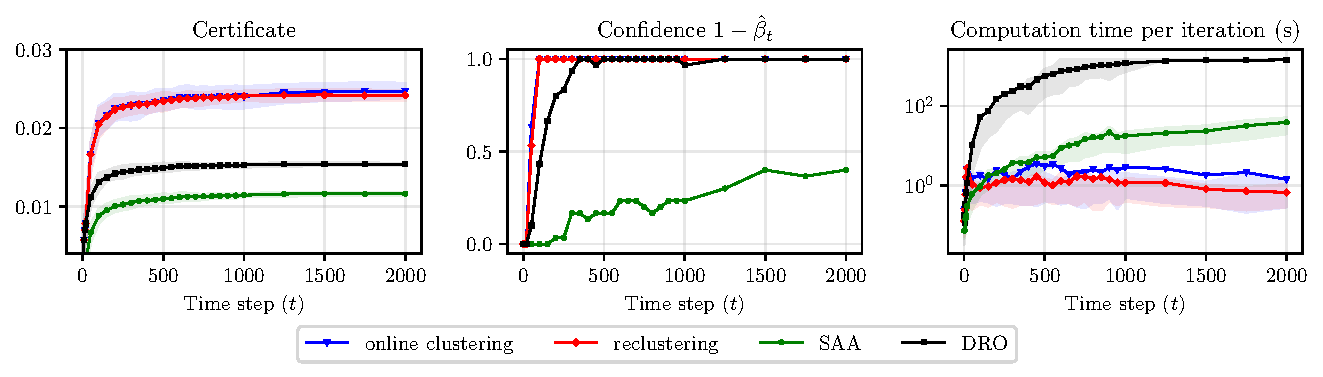
\includegraphics[width = \textwidth]{obj_analysis25.pdf}
	\caption{Sparse portfolio, $K=25$. In-sample certificates, empirical confidence, and per-iteration computation times for the different methods, at $\eps_t = 0.0025{(t+n_0)^{-1/40}}$.}%
	\label{fig:port_obj}%
    
\end{figure}
\begin{figure}[ht]%
\vspace{-0.2em}
	\centering
  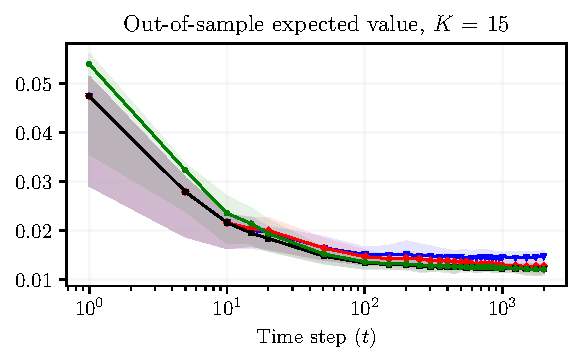
\includegraphics[width = 0.45\textwidth]{eval_analysis_15.pdf}
  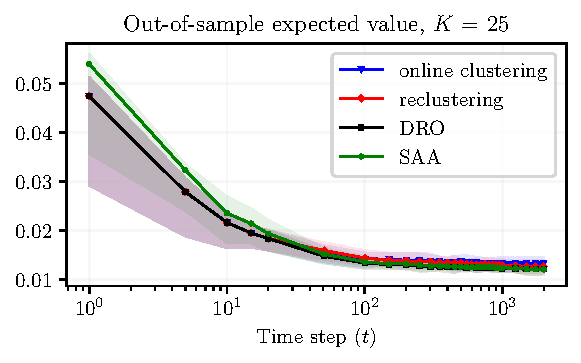
\includegraphics[width = 0.45\textwidth]{eval_analysis_25.pdf}
	\caption{Sparse portfolio. Left: $K = 15$, right: $K = 25$. Out-of-sample expected values for $\epsnom_t = 0.0025{(t+n_0)^{-1/40}}$.}%
	\label{fig:port_eval}%
     
    
\end{figure}
\paragraph{Results}
\RC{For all~\gls{DRO} settings, the radius we obtain through cross-validation is  $\epsnom_t = 0.0025{(t+n_0)^{-1/40}}$.
In Figure~\ref{fig:port_obj}, we compare the certificates, empirical confidence, and per-iteration computation times at the chosen $\epsnom_t$ sequence, and in Figure~\ref{fig:port_eval}, compare the out-of-sample performance. 
We observe that our online data-compressed approaches introduce slight sub-optimality in out-of-sample performance, but provide high-confidence certificates, and offer significant speed-ups compared to nominal~\gls{DRO}. 
As expected, $K=25$ clusters out-performs $K=15$ clusters, but $K=15$ already gives a good approximation of the nominal \gls{DRO} performance.
% For all methods, initializing with a smaller dataset results in worse initial performances, though the robust approaches are able to obtain a good certificate relatively fast. 
The~\gls{SAA} approach improves in performance as the number data points increases, but does not offer a certificate of optimality: the empirical confidence is near 0 for all $t$. Furthermore, it also grows in complexity with sample size and is less efficient than our online approaches. In the long-term, the computation times for our data-compressed approaches can be multiple orders of magnitude faster than that of both~\gls{SAA} and nominal~\gls{DRO}. 
% Surprisingly, as $K=15$ allows for a smaller choice of $\epsnom_t$, the solution times are faster than that of $K=5$. 
We find that the $k$-means warm-starting algorithm (reclustering approach) is particularly efficient, achieving lower computation times and better solution quality than the online clustering method, which entails an extra trade-off between optimality and memory efficiency. Nonetheless, the differences are minimal.}
% We observe that the $k$-means warm-starting algorithm (reclustering approach) is especially efficient, with a lower computation time than even the online clustering approach. The reclustering approach also outperforms the online clustering approach in solution quality, as the latter introduces an additional trade-off between optimality and memory-efficiency. However, the differences in the certificates are minimal. 

\RC{In Figure~\ref{fig:port_regret}, we show the various certificates given in equation~\eqref{eq:is_bounds} (disregarding~$\rho_t$ in favor of cross-validation), and note that the relationships follow the hierarchy presented. The data-compressed in-sample objective value for this maximum-of-affine problem is lower than the in-sample objective of nominal~\gls{DRO}, but adding the clustering discrepancy makes it a valid certificate. We also show the clustering values for a longer horizon, up to $T=10000$, with $\tau = 8500$. 
We observe that the $\barp=1$ and $\barp=2$ clustering discrepancies, $\ld^K_{t,1}$ and $(D^K_{t,2})^2$, as well as $\Phi^K_t$, are converging. 
Moreover, $\ld^K_{t,1} \ge \Phi^K_t$ and, hence, $\max_{j\leq J}M_j\ld^K_{\star,1} \ge \Phi^K_t$  where the maximum Lipschitz constant is $M_1 = 1/\omega = 5$.} This illustrates the relative optimality of $\Phi^K_t$, as opposed to the Wasserstein-1 distance, as proven in Theorem~\ref{cor:opt_cluster}.  
In fact, although we have not assumed (or achieved) optimal clustering-induced coupling, the result still held.
\begin{figure}[ht]%
\vspace{-0.8em}
	\centering
  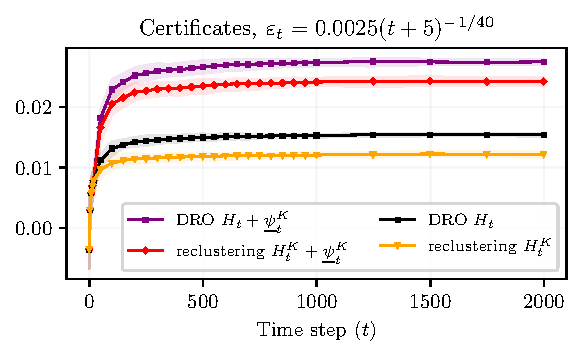
\includegraphics[width = 0.45\textwidth]{bounds_analysis.pdf}
  % 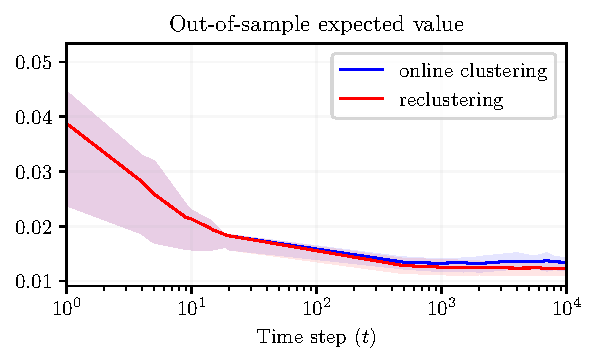
\includegraphics[width = 0.3\textwidth]{eval_analysis_T.pdf}
 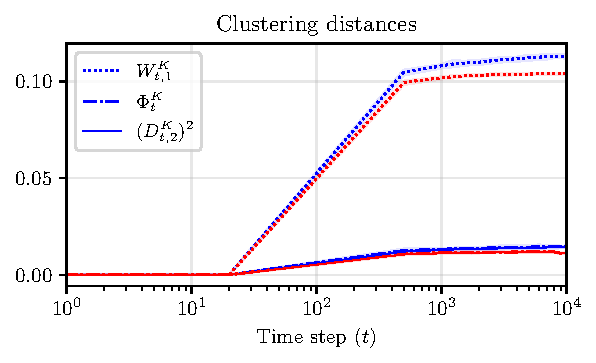
\includegraphics[width = 0.45\textwidth]{dist_conv_W.pdf}
	\caption{Sparse portfolio, $K = 25$. The radius $\epsnom_t = 0.0025{(t+n_0)^{-1/40}}$ for all methods.  Left: certificates from~\eqref{eq:is_bounds}. 
   Right: clustering discrepancies given in Definition~\ref{def:cluster_value}, with $T= 10000$. The lighter (red) shade is for the reclustering method. }%
	\label{fig:port_regret}%
     
    
\end{figure}




% \ifpreprint
% In Figure~\ref{fig:port_regret}, we show the various certificates given in equation~\eqref{eq:is_bounds}, and note that the relationships follow the hierarchy presented. The data-compressed in-sample objective value for this maximum-of-affine problem is lower than the in-sample objective of nominal~\gls{DRO}, but adding the clustering discrepancy makes it a valid certificate.
% % As shown, the upper bounds are generally conservative. Therefore, in practice we tune $\epsnom_t$ using the in-sample value $H^K_t$ instead.  
% \begin{figure}[ht]%
% \vspace{-0.8em}
% 	\centering
%   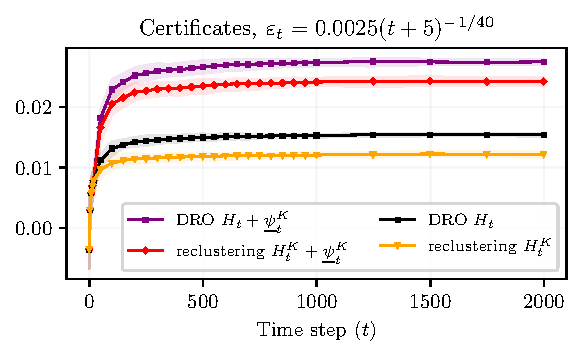
\includegraphics[width = 0.49\textwidth]{bounds_analysis.pdf}
%   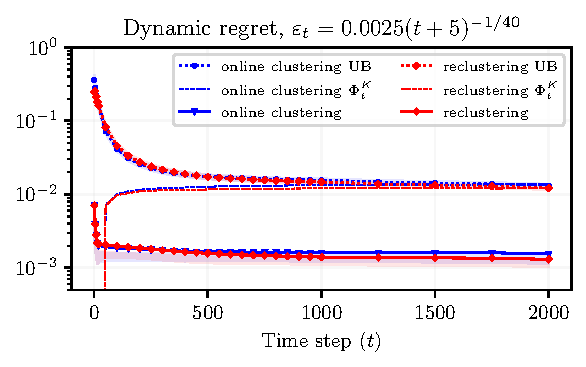
\includegraphics[width = 0.49\textwidth]{regret_analysis.pdf}
% 	\caption{Sparse portfolio, $K = 25$. The radius $\epsnom_t = 0.0025{(t+n_0)^{-1/40}}$ for all methods.  Left: certificates from~\eqref{eq:is_bounds}. 
%     Right: dynamic regret~\eqref{regret}, compared to the theoretical upper bounds.}%
% 	\label{fig:port_regret}%
%     \ifpreprint 
%     \else
%     \vspace{-1em}\fi
% \end{figure}
% In Figure~\ref{fig:port_regret}, we also show the dynamic regret $R(T,K)$ and the regret bound as calculated in Lemma~\ref{lem:regret}. As $T\to\infty$, the upper bound is expected to converge to a fixed function of the clustering discrepancy; indeed, we observe that it coincides with $\Phi^K_t$.
% % converges to $\Phi^K_\star$. 
% This is in line with the theory; since we are solving a maximum-of-affine problem, the term $\bar{\psi}^K_t$ is reduced to 0. 
% \fi
% \ifpreprint 
% The limiting distance becomes $\Phi^K_t$, which, as we show in Figure~\ref{fig:converge} below, is a tighter bound than the Wasserstein-1 distance. This value should converge to its theoretical limit $\Phi_\star^K$.
% \begin{figure}[ht]%
% \vspace{-0.5em}
% 	\centering
%      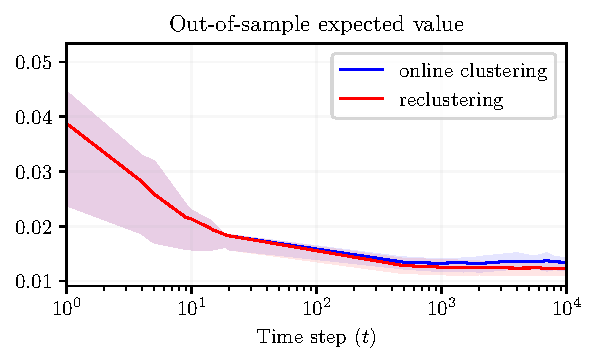
\includegraphics[width = 0.49\textwidth]{eval_analysis_T.pdf}
%  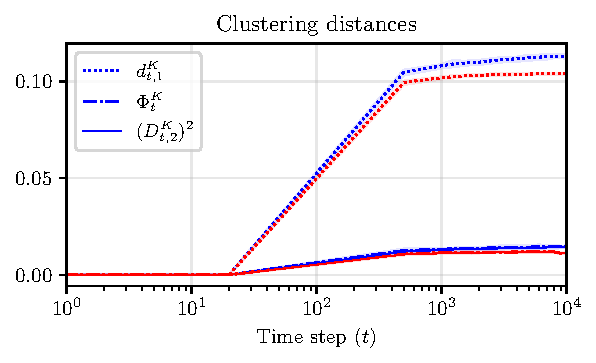
\includegraphics[width = 0.49\textwidth]{dist_conv.pdf}
% 	\caption{Sparse portfolio, $K = 25$, $T=10000$, at $\epsnom_t = 0.0025{(t+n_0)^{-1/40}}$. Left: in-sample certificates. Right: clustering distances given in Definition~\ref{def:cluster_value}.}%
% 	\label{fig:converge}%
%         \ifpreprint \else\vspace{-1em}\fi
% \end{figure}

% In Figure~\ref{fig:converge}, we show the results of our online approaches for a longer horizon, up to $T=10000$, with $\tau = 8500$. 
% We observe that the $\barp=1$ and $\barp=2$ clustering distances, $d^K_{t,1}$ and $(D^K_{t,2})^2$, as well as $\Phi^K_t$, are converging, and the out-of-sample performances are also converging in mean. 
% As remarked above, we observe that $d^K_{t,1}$ upper bounds $\Phi^K_t$ without even multiplying by the maximum Lipschitz constant (which is $1/\alpha = 5$). This illustrates the relative optimality of $\Phi^K_t$, as opposed to the Wasserstein-1 distance, as proven in Theorem~\ref{cor:opt_cluster}.  
% In fact, although we have not assumed (or achieved) optimal clustering-induced coupling, the result still held.
% % \else 
% % The limiting distance becomes $\Phi^K_t$, which, for this example, is a tighter bound than the Wasserstein-1 distance.
% \fi
% % Again, the online clustering approach is slighty suboptimal compared to reclustering, due to the additional trade-off between optimality and memory-efficiency. 
% % However, it still provides a good approximation. 



% \begin{figure}[ht]%
% 	\centering
%  \includegraphics[width = \textwidth]{time_iters.pdf}
% 	\caption{Sparse portfolio, $K = 15$, $n_0=50$. Per-iteration and cumulative computation times for the different methods, at the sequences of $\eps_t$ given in Table~\ref{tab:eps}. The total time for the certificate $\hat{H}^K_t$ is the sum of both reclustering times. \bnote{just plot total time in red}. \bnote{remove cumulative time. remove out of sample plots}}%
% 	\label{fig:port_time}%
% \end{figure}


\section{Conclusions}
\label{c3:sec:conclusions}
We have introduced an online data compression framework for solving Wasserstein~\gls{DRO} problems with streaming data, extending our framework in Chapter~\ref{chap:mro}. 
Our method constructs adaptive ambiguity sets using online clustering, allowing the uncertainty model to evolve as new data arrives, while also maintaining out-of-sample performance guarantees. 
We have analyzed the impact of data compression on solution quality, providing finite-sample and asymptotic performance bounds that relate to nominal bounds for Wasserstein~\gls{DRO}, as well as a sublinear regret analysis with respect to the full-information \gls{DRO} solution. 
The framework is compatible with a broad class of clustering algorithms and supports efficient, memory-aware implementations. 
Numerical experiments in sparse portfolio optimization demonstrate significant computational savings with minimal loss in solution quality.

\chapter{Learning Decision-Focused Uncertainty Sets in Robust Optimization}
\label{chap:lro}

\glsresetall

\section{Introduction}
\label{sec:intro_p}
% Over the past years, \gls{RO} has become a widely adopted efficient tool for decision-making under uncertainty.
% A robust approach first defines an uncertainty set where the uncertain vector lives, and subsequently hedges its decision against any worst-case realization in this set~\citep{robustconvexopt,ben-tal_robust_2009,bertsimassurvey,robustadaptopt}.
As mentioned in Chapters~\ref{chap:intro} and~\ref{chap:prelim}, to attain proper solution quality and practical robustness, the choice of the uncertainty set in \gls{RO} is paramount. Uncertainty sets obtained through a two-step procedure, where information on the optimization problem is not used, could lead to conservative decisions. 
In this chapter, we thus explore an end-to-end approach to build problem-specific uncertainty sets. We additionally consider a {\it context parameter}, such that our results can be applied for a {\it family} of related optimization problems.

We note that the sets considered in Chapters~\ref{chap:mro} and~\ref{chap:online_dro} follow the traditional two-step procedure, but can be enhanced using the results of this chapter. 
Lastly, instead of the function $\ell$ considered in Chapter~\ref{chap:prelim}, in this chapter we work with {\it both} an uncertain objective $f$ and an uncertain constraint $g$. 
% Coverage-based uncertainty sets,


\subsection{Our contributions}%
\label{c4:sub:our_contributions}
In this work, we propose a end-to-end approach to calibrate uncertainty sets for a family of contextual optimization problems, optimizing over a performance metric for the specific problem family.
This is a common scenario in many applications, including inventory management, where we solve similar optimization problems with varying prices and factors driving demand (\ie, context parameters), while satisfying the uncertain demand with high probability.
We construct the uncertainty set, which maps from contexts to context-based regions of uncertainty, by learning its contextual shape and size parameters.
By directly taking into account the quality of the \gls{RO} solutions through the performance metric,
% solving a {family} of parametric \gls{RO} problems and learning the uncertainty set geared towards the specific family, 
the learned set is {\it decision-focused} and eliminates the unnecessary conservatism common in existing data-driven \gls{RO} methods. 
% \RC{In fact, the decision-focused uncertainty sets are calibrated specifically for a given performance metric.
\RC{Our specific contributions are as follows:}
\begin{itemize}
\item 
% \bsnote{We minimize for what? We should say that to train the uncertainty sets, we do the following. This is a point of confusions (difference between training and RO problems) that one of the reviewers raised as well} 
We control the trade-off between performance and robustness by constructing a constrained learning problem for the uncertainty set parameters. 
We minimize the expectation of a performance metric, which incorporates both worst-case and average-case performance, over the family of parametric \gls{RO} problems while ensuring an appropriate probability level of constraint satisfaction. The latter is enforced as a constraint on the conditional-value-of-risk ($\CVaR$) of the problem family's uncertain constraints.
% , which are reformulated into a single joint maximum-of-concave constraint. 
% By incorporating both worst-case and average-case performance as well as data-driven constraint satisfaction into the training problem, we control the trade-off between performance and robustness explicitly.
\item We present the learning problem as a constrained bi-level problem, where the outer level is given above, and the inner level is represented by the family of parametric \gls{RO} problems. The outer level performance metric and $\CVaR$ constraint rely on the solutions of the inner level problems. 
% The aforementioned performance metric and constraints rely on the solutions of the parametric \gls{RO} problems. The overall training formulation 
% \bsnote{formulation of the RO or training problem? specify} 
% is thus a constrained bi-level problem, with the inner level represented by the parametric \gls{RO} problems. 
	% \item We formulate the problem of finding the uncertainty set using bi-level optimization. \bsnote{I would stress the constrained learning setup first, which is already quite challenging to grasp. Then, we can mention that we rely on the inner robust problem solution, essentially solving a bi-level problem.} At the outer level, we minimize the expectation of the objective function over the family of parametric optimization problems, while ensuring an appropriate probability level of constraint satisfaction. At the lower level, we represent the decisions as the solution of the resulting \gls{RO} problem.
 \item We develop a stochastic augmented Lagrangian algorithm to solve the constrained learning problem, which requires differentiating through the inner level solutions as well as the $\CVaR$ constraint. Due to the potentially nonsmooth, nonconvex, and thus nondifferentiable nature of the problem, we show {\it path-differentiability} of the Lagrangian, and apply nonsmooth implicit differentiation. We show convergence to a critical point under step-size and boundedness conditions, and establish the critical point as a feasible solution of the constrained learning problem under mild assumptions. 
 \item Using empirical process theory, we give both marginal and conditional finite sample probabilistic guarantees of constraint satisfaction for the resulting solution.
%  \item We extend our probabilistic guarantees to the case of conditional expectation, where the problem is conditioned on a particular context within the problem family.
 % \bsnote{we need to say that we show convergence and say to what and under which conditions.}
% for the uncertainty sets learned through the aforementioned procedure.
	% \item We introduce a gradient-based approach to learn the optimal $\epsilon$, the radius of generalized uncertainty sets, without the need for any structural information on the underlying distribution.
	% \item Through extending the above approach, we learn something even more powerful -- a set of parameters $(A, b)$ that $\mathit{reshapes}$ the uncertainty sets. Not only does $A$ mimic the $\epsilon$ approach when set to be a scaled identity matrix, it offers improved performances when faced with irregularly shaped distributions.
	% \item We implement our technique in Python package \gls{LROPT}, which allows users to easily model and tune uncertainty sets in \gls{RO}. The code is available at \url{https://github.com/stellatogrp/lropt}.
 % \bsnote{I would not mention the package. I would simply mention the link to the experiments repo at the end of the bullet point below where we talk about the experiments. This is not a pakcage paper.}
 \item Our uncertainty sets are highly tractable, as they are based on 
a variety of traditional sets with simple structure, such as ellipsoidal and budget sets. 
% Once the uncertainty set parameters are learned, we obtain a highly tractable formulation.
% as developed in~\cite{bertsimas_data-driven_2018}, or \gls{DRO} uncertainty sets, which require larger problem formulations.}
\item We benchmark our method on examples in portfolio optimization and multi-stage inventory management, outperforming data-driven robust and distributionally robust approaches in terms of out-of-sample performance and probabilistic guarantees. The code is available at \githubrepo.
\end{itemize}
% shape, size instead of epsilon, geometry instead of A,b

% \subsection{Related work}%
% \label{c4:sub:related_work}

% \paragraph{Risk measures.}
% Value at risk ($\mathbf{VaR}$) and conditional value at risk ($\CVaR$) are common risk measures for quantifying costs encountered in the tails of distributions.
% A $\mathbf{VaR}_\eta$ constraint is a chance constraint that measures the maximum cost incurred with respect to a given confidence level $\eta$, but while intuitive, the function is often intractable, and does not quantify costs beyond the found threshold value.
% \RC{Conditional value at risk, on the other hand, measures the {\it expected} cost given that the cost exceeds $\mathbf{VaR}$, and, as the tightest convex approximation of $\mathbf{VaR}$, is known to have a tractable formulation~\citep{cvaropt,cvar}. }
% Since its development, $\CVaR$ optimization has been a common method for controlling risk in portfolio optimization and option hedging problems, and has also been explored in risk-constrained Markov decision problems, where the risk is presented as a constraint on the $\CVaR$ of the cumulative cost~\citep{cvar_markov}.
% \RC{In fact, $\CVaR$ is a {\it coherent risk metric}~\citep{coherentrisk}, which satisfies certain axioms that give it value beyond approximating the $\VaR$~\citep{cvar_var}.}
% The use of $\CVaR$ constraints to substitute chance constraints has also been explored in reliability engineering, where the $\CVaR$ constraint has been given a different name: buffered failure probability~\citep{buffered}.
% In our work, we constrain risk, which in \gls{RO} is the probability of constraint violation, by constraining the $\CVaR$ of the uncertain constraint functions.

\subsection{Layout of the paper}%
\RC{In Section~\ref{c4:sec:intro}, we introduce the notion of the decision-focused set with a motivating example. In Section~\ref{sec:learn}, we describe the data-driven algorithm and prove its convergence, and in Section~\ref{sec:guarantees}, provide probabilistic guarantees.
% In Section~\ref{sec:HL_canon}, we give a high-level overview of our \gls{LROPT} package, and 
In Section~\ref{sec:hyper}, we discuss hyperparameter tuning, and in Section~\ref{c4:sec:examples}, present various numerical examples problems.}
For completeness, we give example convex reformulations of robust optimization problems for common uncertainty sets, with our shaped parameters, in the appendices.
% \bsnote{make sure this matches the final version after we move things to fit journal page limits}

\section{The optimization problem}
\label{c4:sec:intro}
Consider a contextual stochastic optimization setting with context parameter $x \in \reals^p$ and uncertain parameter $u \in \reals^m$. 
The context parameter $x$ represents information available when we make our decisions (\eg, market factors for portfolio optimization, the supplier's price for inventory problems), while the uncertain parameter $u$ is not known (\eg, future returns in portfolio optimization), but may be affected by the context parameter.
We set $\prob_x$ as the distribution of $x$ with domain $\mathcal{D}_x \subseteq \reals^p$, $\prob_u$ as the  distribution of $u$ with domain $\mathcal{D}_u \subseteq \reals^m$, and $\prob_{(u, x)}$ as their joint distribution, all of which are unknown.
Importantly, since $x$ may affect $u$, $u$ and $x$ can be correlated. We therefore denote by $\prob_{(u|x = \bar{x})}$ the conditional distribution of $u$ for a context $\bar{x} \in \mathcal{D}_x$.

\subsection{The conditional formulation}
\label{sec:cond}
For any context $\bar{x}$, the decision-maker, who has some uncertain objective function $f(z,u,\bar{x})$, would like to ensure that their decision $z(\bar{x}) \in \reals^n$ performs well in both the average-case and the worst-case, where we use the following {\it value at risk} formulation to describe the $\eta$-quantile worst-case. That is, for some risk parameter $\eta \in [0,1]$:
\begin{equation*}
\VaR(f(z(\bar{x}),u,\bar{x}),\eta|\bar{x}) = \inf\{\Gamma \mid \prob_{(u|x = \bar{x})}(f(z(\bar{x}),u,\bar{x}) \leq \Gamma) \geq 1-\eta\} \leq 0.
\end{equation*} 
The decision-maker would then consider minimizing the aggregate objective,
\begin{equation}
	\label{eq:performance_metric}
	\Expect_{(u|x = \bar{x})}\left(\hat{\Phi}_\gamma(z(\bar{x}),u,\bar{x})\right) = \Expect_{(u|x = \bar{x})}\left(\gamma f(z(\bar{x}),u,\bar{x}) + \VaR(f(z(\bar{x}),u,\bar{x}),\eta|\bar{x}) \right),
\end{equation} 
where the first term describes the average-case, the second term describes the worst-case, and $\gamma$ controls their tradeoff. This dual objective is inspired by the developments on Pareto-optimal solutions by~\cite{pareto}, who identify solutions for \gls{RO} problems that perform well not only in the worst-case, but also dominates all other solutions in the typical-case. 

Ideally, the problem for any context $\bar{x} \in \mathcal{D}_x$ can then be formulated as
\begin{equation}
	\label{eq:bilevel_intro_opt_cond}
	\begin{array}{ll}
		\underset{z(\bar{x})}{\mbox{minimize}} & \Expect_{(u|x = \bar{x})}\left(\hat{\Phi}_\gamma(z(\bar{x}),u,\bar{x})\right) \\
		\mbox{subject to} & \VaR(\hat{g}(z(\bar{x}),u,\bar{x}),\eta|\bar{x}) \leq 0,\\
	\end{array}
\end{equation}
where the function $\hat{g} : \reals^n \times \reals^m \times \reals^{p} \to \reals$  is an {\it uncertain constraint} the decision-maker might have, and would like to constrain below 0 with high probability (that is, with probability $1-\eta$, as implied by the value at risk constraint). We assume $\hat{g}$ to be the maximum of functions concave in $u$ and convex in $z$ and $x$,~\eg, $\hat{g}(z, u, x) = \max_{l=1,\dots, \hat{L}} \hat{g}_l(z, u, x)$. This structure allows us to express $\hat{L}$ joint uncertain constraints using the maximum of each component $l$. Similarly, we assume the original objective function $f$ to be concave in $u$ and convex in $z$. 

With these assumptions, we can in fact move the $\VaR$ in the peformance metric~\eqref{eq:performance_metric} into the constraint, that is, define 
\begin{align*}
\Phi_\gamma(z(\bar{x}),u,\bar{x}) &= \gamma f(z(\bar{x}),u,\bar{x}) + t(z(\bar{x}))\\
g(z(\bar{x}),u,\bar{x}) &= \max\{f(z(\bar{x}),u,\bar{x}) - t(z(\bar{x})),\hat{g}(z(\bar{x}),u,\bar{x})\},
\end{align*}
where $z(\bar{x})$ is augmented with an additional epigraph variable, and the function $t(z(\bar{x}))$ extracts this epigraph variable. Furthermore, the new constraint $g$ is an augmentation of the original constraint $\hat{g}$ with the epigraph constraint $f(z(\bar{x}),u,\bar{x}) - t(z(\bar{x})) \leq 0$, with the number of concave pieces now $L = \hat{L}+1$.
% Then, if we consider the constraint $g$ to incorporate the function $ \leq 0$ as one of the $L$ components of the maximum, we arrive at an equivalent formulation. 
For the rest of the paper, we assume to work with this transformed formulation. The corresponding formuation of~\eqref{eq:bilevel_intro_opt_cond} becomes
\begin{equation}
	\label{eq:bilevel_intro_opt_cond_new}
	\begin{array}{ll}
		\underset{z(\bar{x})}{\mbox{minimize}} & \Expect_{(u|x = \bar{x})}\left(\Phi_\gamma(z(\bar{x}),u,\bar{x})\right) \\
		\mbox{subject to} & \VaR(g(z(\bar{x}),u,\bar{x}),\eta|\bar{x}) \leq 0.\\
	\end{array}
\end{equation}

The conditional formulation given in~\eqref{eq:bilevel_intro_opt_cond_new} is powerful, as the constraint controls the risk for each context. However, while the conditional guarantee is desirable, in real-life settings the conditional distribution may be difficult to estimate~\citep{conformal}. The associated performance guarantees require stringent assumptions, which additionally depend on the approximation technique applied. While we do provide performance guarantees for this setting (see Section~\ref{sec:cond_guarantee}), for the sake of simplicity, we focus on the following {\it joint formulation},
\begin{equation}
	\label{eq:bilevel_intro_opt_cond_joint}
	\begin{array}{ll}
		\underset{z(\cdot)}{\mbox{minimize}} & \Expect_{(u,x)}\left(\Phi_\gamma(z(x),u,x)\right) \\
		\mbox{subject to} & \VaR(g(z,u,x),\eta) \leq 0,\\
	\end{array}
\end{equation}
which can be interpreted as~\eqref{eq:bilevel_intro_opt_cond_new} with an additional expectation taken over $x$ in both the objective and the constraints. Instead of optimizing for a particular context, we want to find a mapping $z(\cdot)$ that performs well {\it across all contexts}. Such a mapping would then be applicable for any context within the problem family.
% Note that while a mapping $z(\bar{x})$ found through~\eqref{eq:bilevel_intro_opt_cond_new} might overfit to the particular context, and would not be applicable for other contexts, the mapping $z(\cdot)$ of~\eqref{eq:bilevel_intro_opt_cond_joint} could be applied for any context within the problem family. 
In the following, we describe our proposed mapping. 

\subsection{The joint formulation and the bi-level problem}
\label{sec:joint}
In~\eqref{eq:bilevel_intro_opt_cond_joint}, we are interested in finding the best mapping $z(\cdot)$ from context parameters $x$ to decisions $z$. To this end, we define the parametic set-valued mapping given by $x \rightarrow \uncset(\theta,x)$, where 
$\uncset(\theta,x) \subseteq \reals^m$ is a convex contextual uncertainty set that depends on the {\it set parameter} $\theta \in \reals^q$.
For example, $\theta$ can represent the mapping between $x$ and the center, size, and shape of~$\uncset(\theta,x)$.
We then define the mapping $z(\cdot)$ as the solution to the \glsfirst{RO} problem
\begin{equation}
	\label{eq:robust_prob}
	z(\theta, x) \in \begin{array}[t]{ll}
		\mbox{argmin}  &t(z)\\
		\mbox{subject to} & g(z,u,x)  \le 0  \quad \forall u \in \uncset(\theta,x).
	\end{array}
\end{equation}
In this manner, we would like to find the optimal parameter $\theta$ by solving the bi-level optimization problem
\begin{equation}
	\label{eq:bilevel_intro_opt_theta}
	\begin{array}{ll}
		\underset{\theta}{\mbox{minimize}} & \Expect_{(u,x)}\left(\Phi_\gamma(z(\theta,x),u,x)\right) \\
		\mbox{subject to} & \VaR(g(z(\theta,x),u,x),\eta) \leq 0,\\
	\end{array}
\end{equation}
where the inner level problems, which becomes constraints of the outer level problem~\eqref{eq:bilevel_intro_opt_theta}, is represented by~\eqref{eq:robust_prob}, for all $x \in \mathcal{D}_x$. 
Problem~\eqref{eq:robust_prob} guarantees that, for $\theta$ and any given $x$, the solution $z(\theta, x)$ satisfies the constraint for any value of the uncertain parameter $u$ in $\uncset(\theta,x)$. The outer level problem~\eqref{eq:bilevel_intro_opt_theta} then selects $\theta$ in a {\it decision-focused} manner, such that the solutions \RC{$z(\theta, x)$} perform well in terms of the performance metric and satisfy the $\VaR$ constraint across the problem class.


% The decision-maker would like to ensure that their decision $z \in \reals^n$ performs well in both average-case and worst-case situations across the contexts $x$ and uncertainty $u$, that is, for some uncertain objective function $f(z,u,x)$,
% both 
% $$\Expect_{(u,x)}\left(f(z(x),u,x)\right)~~~\text{and}~~~\Expect_{x}\left(t(x)\right)~~\text{such that}~~\prob_{(u,x)}(f(z(x),u,x)\leq t(x)) \geq 1 - \eta$$
% are taken into consideration.
% Here, the variable $z(x)$ denotes the decision made for the context $x$, and the variable $t(x)$ is constructed to represent the corresponding $\eta$-quantile worst-case objective value for the context $x$, for some risk parameter $\eta \in [0,1]$. 
% This dual objective is inspired by the developments on Pareto-optimal solutions by~\cite{pareto}, who identify solutions for \gls{RO} problems that perform well not only in the worst-case, but also dominates all other solutions in the typical-case. 

% In this formulation, $\prob_x$ is the distribution of $x$ with domain $\mathcal{D}_x \subseteq \reals^p$, $\prob_u$ is the  distribution of $u$ with domain $\mathcal{D}_u \subseteq \reals^m$, and $\prob_{(u, x)}$ is their joint distribution, all of which are unknown.
% Importantly, $u$ and $x$ can be correlated.
% We note that this is an aggregate probabilistic guarantee for the parametric class of problems, and not a conditional guarantee which holds for all instances~$x$. 
% Whereas a conditional guarantee is more desirable, there are multiple methods through which we can approximate the conditional distribution~\citep{bertsimas2020predictive}, each with its own required assumptions. While our results can extend to such settings, to avoid cumbersome exposition in the main text, we delay these extensions to Appendix~\ref{appx:conditional}. In the rest of the section, we work with the joint distribution $\prob_{(u, x)}$.



% % stringent assumptions on the distribution \RC{$\prob_x$}, which are typically hard to verify in practice~\citep{condcover}~\citep[Section 3.1]{conformal}.}


% Ideally, the problem can then be formulated as
% \begin{equation}
% 	\label{eq:bilevel_intro_opt}
% 	\begin{array}{ll}
% 		\underset{z(\cdot)}{\mbox{minimize}} & \Expect_{(u,x)}\left(\Phi_\gamma(z(x),u,x)\right) \\
% 		\mbox{subject to} & \prob_{(u,x)}(g(z(x),u,x) \le 0) \ge 1 - \eta,\\
% 	\end{array}
% \end{equation}
% where the performance metric  $\Phi_\gamma(z(x),u,x) = t(z(x)) + \gamma f(z(x),u,x)$ consolidates the two objectives through the tunable hyper-parameter $\gamma$. Note that with a slight abuse of notation, we assume now that the epigraph variable $t(x)$ constructed is within $z(x)$, such that $t(z(x))$ extracts this epigraph variable from $z(x)$. 
% The function $g : \reals^n \times \reals^m \times \reals^{p} \to \reals$  is an uncertain constraint which we assume to be the maximum of functions concave in $u$ and \RC{convex in $z$ and $x$,~\eg, $g(z, u, x) = \max_{l=1,\dots, L} g_l(z, u, x)$.}
% This structure allows us to express $L$ joint uncertain constraints using the maximum of each component $l$. We note that the constraint $f(z(x),u,x)- t(z(x)) \leq 0$ is assumed to be encoded into $g$ as one of the components. 
% % We note that linear adjustable \gls{RO} problems with affine decision rules also fall within this class.




% In~\eqref{eq:bilevel_intro_opt}, we are interested in finding the best mapping $z(\cdot)$ from context parameters $x$ to decisions $z$. To this end, we define the parametic family of set-valued mappings given by $x \rightarrow \uncset(\theta,x)$, where 
% $\uncset(\theta,x) \subseteq \reals^m$ is a convex contextual uncertainty set that depends on the {\it set parameter} $\theta \in \reals^q$.
% For example, $\theta$ can represent the mapping between $x$ and the center, size, and shape of~$\uncset(\theta,x)$.
% We then define the mapping $z(\cdot)$ as the solution to the \glsfirst{RO} problem
% \begin{equation}
% 	\label{eq:robust_prob}
% 	z(\theta, x) \in \begin{array}[t]{ll}
% 		\mbox{argmin}  &t(z)\\
% 		\mbox{subject to} & g(z,u,x)  \le 0  \quad \forall u \in \uncset(\theta,x).
% 	\end{array}
% \end{equation}
% In this manner, we would like to find the optimal parameter $\theta$ by solving the bi-level optimization problem
% \begin{equation}
% 	\label{eq:bilevel_intro_opt_theta}
% 	\begin{array}{ll}
% 		\underset{\theta}{\mbox{minimize}} & \Expect_{(u,x)}\left(\Phi_\gamma(z(\theta,x),u,x)\right) \\
% 		\mbox{subject to} & \prob_{(u,x)}(g(z(\theta,x),u,x) \le 0) \ge 1 - \eta,\\
% 	\end{array}
% \end{equation}
% where the inner level problem is represented by~\eqref{eq:robust_prob}.
% Problem~\eqref{eq:robust_prob} guarantees that, for $\theta$ and any given $x$, the solution $z(\theta, x)$ satisfies the constraints for any value of the uncertain parameter $u$ in $\uncset(\theta,x)$. The outer level problem~\eqref{eq:bilevel_intro_opt_theta} then selects $\theta$ in a {\it decision-focused} manner, such that the solutions \RC{$z(\theta, x)$} perform well in terms of the performance metric and satisfy the chance constraint across the problem class.

% Unfortunately, as the chance constraint is intractable, this problem cannot be solved directly. A common reformulation technique is to
% express the chance constraint in~\eqref{eq:bilevel_intro_opt_theta} in terms of the corresponding {\it value at risk}, \ie,
% \RC{\begin{equation*}
% \VaR(g(z(\theta,x),u,x),\eta) = \inf\{\Gamma \mid \prob_{(u,x)}(g(z(\theta,x),u,x)\leq \Gamma) \geq 1-\eta\} \leq 0.
% \end{equation*}}

Unfortunately, the value at risk function often leads to intractable formulations~\citep{cvaropt}, so our problem cannot be solved directly. 
To get a tractable approximation, we adopt the {\it conditional value at risk}~\citep{cvaropt,cvar}, defined as
\begin{equation*}
	\label{eq:cvar}
\CVaR(g(z(\theta,x),u,x),\eta) = \inf_{\alpha}\left\{\frac{\Expect_{(u,x)} (g(z(\theta,x),u,x)- \alpha)_+}{\eta} + \alpha\right\},
\end{equation*}
where $(a)_+ = \max\{a,0\}$. It is well known~\citep{cvaropt} that, for any \RC{$z \in \reals^n$}, the relationship between these probabilistic guarantees of constraint satisfaction is
% Please use quad instead of specific hspace cm. Otherwise, if we change the layout, things can break.
\begin{equation*}
	\label{eq:imply}
\CVaR(g(z,u, x),\eta) \leq 0 ~~\Longrightarrow~~ \VaR(g(z,u,x),\eta)\leq 0 ~~\Longleftrightarrow ~~ \prob_{(u,x)}(g(z,u,x)\leq 0) \geq 1 - \eta.
\end{equation*}
Therefore, if the solution \RC{$z(\theta,x)$ of~\eqref{eq:robust_prob} satisfies $\CVaR(g(z(\theta,x),u,x),\eta) \leq 0$,} we have the desired probabilistic guarantee in~\eqref{eq:bilevel_intro_opt_theta}.
In fact, as the $\CVaR$ constraint is stronger than the $\bf{VaR}$ constraint, ensuring its satisfaction might result in more desirable solutions, especially when, on top of the {\it threshold} worst-case value, the decision-maker is concerned with the {\it magnitude} of all the worst-case values beyond the threshold~\citep{cvar_var}. Furthermore, this formulation should not favor neglecting certain contexts $x$ (such that they suffer constraint violations of a significant magnitude) in exchange for better performance for other contexts, since that would result in a high $\CVaR$.


\subsection{Data-driven approximation}
\label{ssec:constrained_learning}
As the distribution $\prob_{(u,x)}$ is unknown, we are unable to obtain the true expectation in~\eqref{eq:bilevel_intro_opt_theta}. We do, however, assume access to historical data.
Suppose we are given
a pair of {\it training} datasets $W^{N} = (U^N,X^N) = \{(u^i,x^i)\}_{i=1}^N \subseteq \mathcal{D}_{(u,x)}$, consisting of a set of $N$ independent samples of the uncertain parameter $u$ and context parameter $x$, governed by $\prob^N$, their joint distribution.
As the true probabilistic guarantee in~\eqref{eq:bilevel_intro_opt_theta} cannot be obtained, we instead target the
% Our main requirement is to identify a set parameter $\theta$ for which the solutions $z(\theta, x)$ to problem~\eqref{eq:robust_prob} with uncertainty set $\mathcal{U}(\theta,x)$, satisfy
the following {\it finite-sample probabilistic guarantee}
\begin{equation}
  \label{eq:prob_guarantee}
  \prob^{N}\left(\prob_{(u,x)}(g(z(\theta,x),u,x) \le 0) \ge 1 - \eta\right)\geq 1 - \beta,
\end{equation}
where $\beta > 0$ is the target confidence level across draws of the dataset $W^N$.
In other words, for any dataset $W^N$ drawn from the true distribution, the learned $\theta$ satisfies the chance constraint $\prob_{(u,x)}(g(z(\theta,x),u,x) \le 0) \ge 1 - \eta$ with confidence $\beta$.
% In other words, we are looking for $\theta$ such that the probability of observing $N$ samples which results in data-driven decisions $z(\theta,x)$ that do not satisfy the desired guarantee is small.
% \bsnote{use only round or curly brackets for probabilities, but do not mix them}
% \bsnote{What do you mean by ``stochastic version of~\eqref{eq:bilevel_intro}''? Isn't that already a stochastic program?}
% Instead of working with the probability $\prob_{(u,x)}$,} which often leads to intractable formulations~\citep{cvaropt} as discussed in Section~\ref{c4:sec:intro}, we adopt a tractable approximation based on the {\it conditional value at risk}~\citep{cvaropt,cvar} defined in~\eqref{eq:cvar}, obtaining the constraint
% \RC{$$\CVaR(g(z(\theta,x),u,x),\eta) \le \kappa \quad \iff\quad \inf_{\alpha}\left\{\frac{\Expect_{(u,x)} (g(z(\theta,x),u,x)- \alpha)_+}{\eta} + \alpha\right\}\leq \kappa,$$}
% where $\kappa > 0$ is a threshold value that we define in Section~\ref{sec:guarantees} to obtain the finite sample guarantees~\eqref{eq:prob_guarantee}.
% \citep{cvaropt}.
% To get a tractable approximation, we can adopt the {\it conditional value at risk}~\citep{cvaropt,cvar}, defined as
% \begin{equation}
% 	\label{eq:cvar}
% \CVaR(g(x(\theta,y),u,y),\eta) = \inf_{\alpha}\{\Expect_{(u,y)}((1/\eta)(g(x(\theta,y),u,y)- \alpha)_+) + \alpha\},
% \end{equation}
% where $(a)_+ = \max\{a,0\}$.
% Here, $u$ are realizations of the constructed uncertainty set, $y$ are the family parameters, and $\prob_{(u,y)}$ denotes the joint distribution of $(u,y)$.
% In order to formalize the learning task, we define an outer problem minimizing the expected value of the objective function $f(x(\theta, y), y)$ of~\eqref{eq:robust_prob}, subject to the following constraint,
% $$\CVaR(g(x(\theta,y),u,y),\eta) \leq \kappa,$$
% where $\kappa \le 0$ is a target value, and the $\CVaR$ is defined as in~\eqref{eq:cvar}. As mentioned in Section~\ref{c4:sec:intro}, this then implies a probabilistic guarantee of constraint satisfaction~\eqref{eq:imply}.
To obtain such a guarantee, we first must ensure the convergence of a data-driven version of~\eqref{eq:bilevel_intro_opt_theta}.
To this end, we define a constraint on the sampled $\CVaR$,
\begin{equation}
\label{eq:sampled_cvar}
\widehat{\CVaR}(\theta) = \inf_{\alpha} \frac{1}{N}\sum_{i=1}^N \left(\frac{(g(z(\theta,x^i),u^i,x^i)- \alpha)_+}{\eta} + \alpha \right)\leq \kappa,
\end{equation}
and require this condition to hold for feasible $\theta$.
\RC{The value $\kappa < 0$ is a threshold margin that we define later in Section~\ref{sec:guarantees}, Theorem~\ref{thm:fin_sample}, to ensure the finite sample guarantee~\eqref{eq:prob_guarantee}.}
\RC{We can then formulate the stochastic objective and constraint functions as follows,}
\begin{equation*}
F(\theta) = \frac{1}{N}\sum_{i=1}^N\Phi_{\gamma}(z(\theta,x^i),u^i, x^i) \quad \text{and}\quad H(\alpha,\theta) = \frac{1}{N}\sum_{i=1}^N ((g(z(\theta,x^i),u^i,x^i)- \alpha)_+/\eta + \alpha - \kappa)_+,
\end{equation*}
evaluated over the dataset 
$W^N$. We use these approximations to define the sampled version of~\eqref{eq:bilevel_intro_opt_theta} as
\begin{equation}
	\label{eq:bilevel_sampled}
	\begin{array}{ll}
		\underset{\alpha,\theta}{\mbox{minimize}} & F(\theta) \\
		\mbox{subject to} & H(\alpha,\theta) = 0,\\
	\end{array}
\end{equation}
where the constraint $H$ corresponds to the $\CVaR$ constraint where $\alpha$ is also a minimization variable.
When the functions $f$ and $g$ are convex in $z$, optimizing over $\alpha$ as well has no impact on the optimal solution~\citep{cvar_ref}.
With this formulation, we thus tune $\alpha$ and the set parameter $\theta$ to improve the quality of the solutions \RC{$z(\theta,x^i)$} of the inner \gls{RO} problem~\eqref{eq:robust_prob}, measured by the performance on the outer level problem.

Solving the stochastic problem~\eqref{eq:bilevel_sampled} is challenging because of the nonconvex bi-level structure introduced by the inner \gls{RO} problem~\eqref{eq:robust_prob}.
While it may be possible to directly reformulate it as a single-level problem, this would involve several bilinear constraints over the entire training dataset, which can be difficult even in the simplest case of $\ell_1$-norm uncertainty sets; see Appendix~\ref{appx:bilinear}.
% Our approach, despite requiring hyperparameter tuning, can be batched for low per-iteration cost. 
We address these challenges in the following section, by introducing a stochastic first-order method to address problem~\eqref{eq:bilevel_sampled} with tractable iterations.
For the high-level architecture, see Figure~\ref{fig:arch}.

\begin{figure}[ht]%
	\centering
	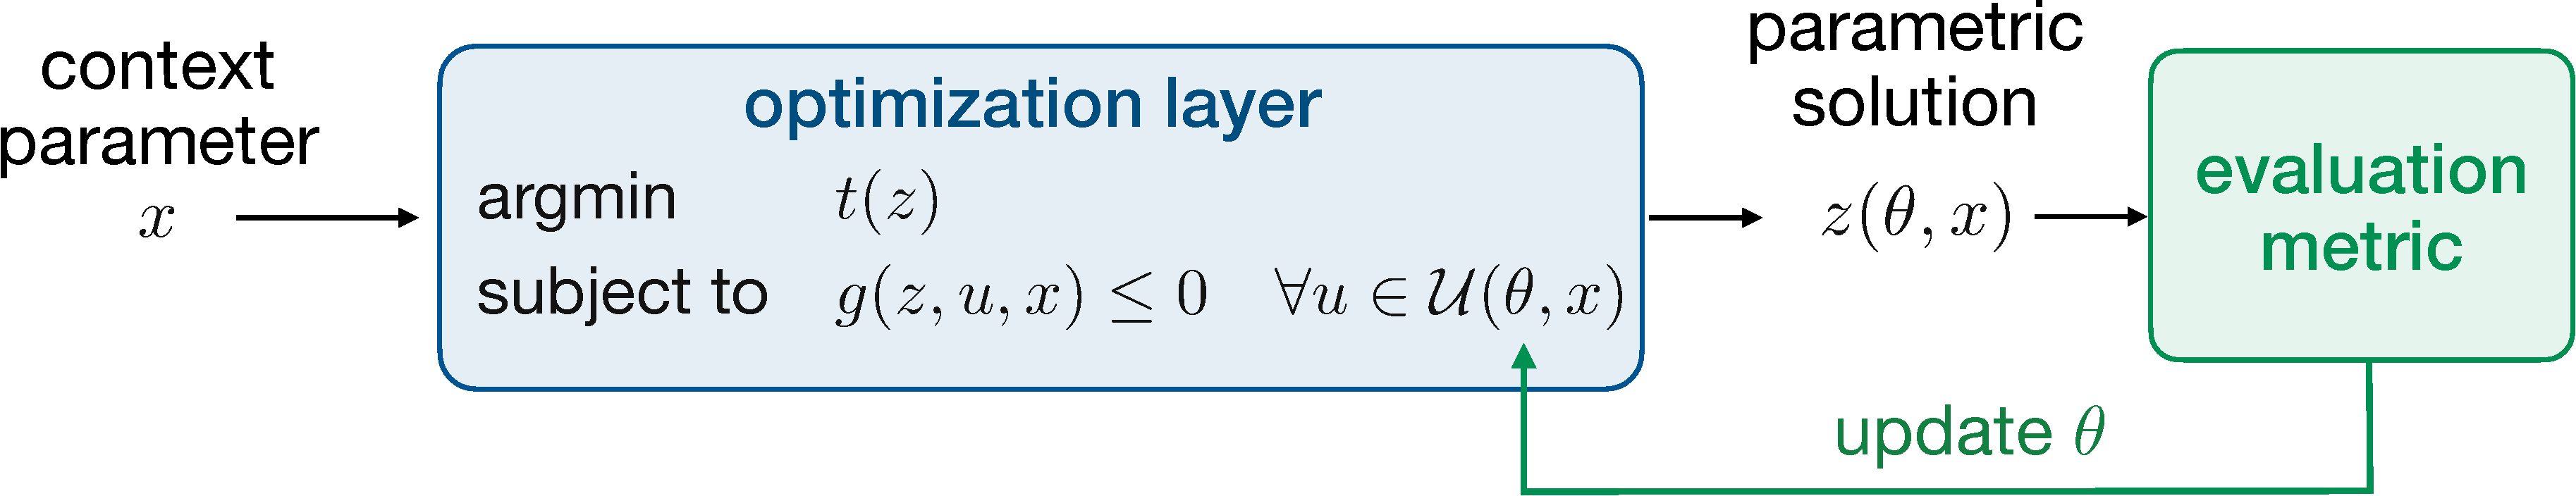
\includegraphics[width=0.7\textwidth]{img_architecture_t.pdf}
	\caption{Our high-level procedure. 
	% We evaluate the performance of the decision $z(\theta,x)$ in terms of the expected objective value and constraint satisfaction. 
	The evaluation metric is the augmented Lagrangian function defined in Section~\ref{sec:training_procedure}, and is derived from the sampled problem~\eqref{eq:bilevel_sampled}.}
	\label{fig:arch}%
    % \ifpreprint\else
    % \vspace{-1em}
    % \fi
\end{figure}

We give in Appendix~\ref{appx:gen_sets} examples of parameterized uncertainty sets and the corresponding convex reformulations of~\eqref{eq:robust_prob}, which we use to solve for \RC{$z(\theta,x^i)$}. 
In the motivating example below, we give a parameterization of an ellipsoidal uncertainty set, where the trainable parameters are $\theta = (W_A, W_b, h_A, h_b,\rho)$. Learning $\theta$ using~\eqref{eq:bilevel_sampled} thus equates to learning a feasible and ideally optimal set-valued mapping from context parameters to a region of uncertainty realizations.


% \bsnote{I would describe the problem here and the desired probabilistic guarantees of constraint satisfaction. 1) this clarifies the goal earlier on, and 2) this makes it easier to follow the motivating example.}
% \RC{We consider a class of parametric \glsfirst{RO} problems, indexed by the {\it context parameter}~$x \in \reals^p$, where each instance takes the form:}
% % Each problem takes the form:
% \RC{\begin{equation}
% 	\label{eq:robust_prob}
% 	z(\theta, x) \in \begin{array}[t]{ll}
% 		\mbox{argmin}  &f(z)\\
% 		\mbox{subject to} & g(z,u,x)  \le 0  \quad \forall u \in \uncset(\theta,x),
% 	\end{array}
% \end{equation}}
% \bsnote{argmin is a set in general, we cannot use equality condition. We either write $x \in \argmin$, or we write $=$ and directly mention that there is a unique optimal solution.}
% \bsnote{I think we can have $f(x)$ simply. It should make things cleaner. I started editing it but we should change other parts as well.}
% where $y \in \reals^{n'}$ parametrizes the family with underlying distribution $\prob_y$,
% \RC{where $z \in \reals^n$ is the optimization variable}, $u \in \reals^m$ is the {\it uncertain parameter}, $f: \reals^n \to \reals$ is the convex objective function, and $g : \reals^n \times \reals^m \times \reals^{p} \to \reals$ is the uncertain constraint which we assume to be the maximum of functions concave in $u$ and \RC{convex in $z$ and $y$,~\eg, $g(z, u, x) = \max_{l=1,\dots, L} g_l(z, u, x)$.}
% \bsnote{Are we using max of concave or max of affine in the end? It looks like we have max of affine.}
% This structure allows us to express $L$ joint uncertain constraints using the maximum of each component $l$.
% \RC{We note that linear adjustable \gls{RO} problems with affine decision rules also fall within this class.}
% \bsnote{is the definable assumption absolutely necessary here to understand? or can we put it in the theorems directly?}
% We refer to {\it instances} of the family as the realization of problem~\eqref{eq:robust_prob} where $y$ takes a specific value.

% \RC{Problem~\eqref{eq:robust_prob} guarantees that, for a given $x$, the solution $z(\theta, x)$ satisfies the constraints for any value of the uncertain parameter $u$ in $\uncset(\theta,x) \subseteq \reals^m$, a convex {\it contextual} uncertainty set that depends on the {\it set parameter} $\theta \in \reals^q$.
% For example, $\theta$ can represent the mapping between $x$ and the center, size, and shape of~$\uncset(\theta,x)$.
% % \bsnote{to be precise, $\theta$ represents the mapping between $x$ and the center,size, etc}
% % maximum-of-concave function in $u$.
% In this setting, the context parameter $x$ represents information available when we make our decisions (\eg, current allocations in portfolio optimization, the price of the products to sell in inventory problems). } The uncertain parameter $u$, however, is not known (\eg, future returns in portfolio optimization). 
% \RC{The context parameter $x$ is allowed to affect the uncertain parameter $u$.}
% Importantly, we do not assume that $y$ affects $u$, which is common in several practical applications (\eg, when our portfolio allocations do no affect future market returns).

% from the uncertain parameter $u$ in that it is known when we make the decision.
% \bsnote{Give a quick example in a inventory problem or portfolio optimization problem, where $y$ and $u$ do not interact.}
% This allows us to exploit the structure of this family of parametric \gls{RO} problems, as we train an uncertainty set specifically targeted for it. 
% particular family.
% , and need not consider the entire class of optimization problems.
% Note that, if $y$ is supported on a single value, we obtain the usual \gls{RO} formulation.
% , whose dimensions depend on the form of the uncertainty set considered (\ie~box, ellipsoidal).
% As learning an uncertainty set is costly, %% One could learn a function (contextual) instead of a different set. I don't think the argument holds here....
% Here, the set $\uncset(\theta)$ does not depend on individual $y$ as this would require either learning a different uncertainty set for every instance of the family, which may be costly, or learning a mapping from $y$ to the uncertainty set (as in conditional \gls{RO}~\citep{contex}), which may be hard to interpret.
% % \bsnote{we should mention the last two points in the lit review}
% Instead, we construct a fixed set that works for all realizations of $y$ encountered in target application.

% Our goal is to find a set parameter $\theta$ in a {\it decision-focused} manner, \ie, such that the solutions \RC{$z(\theta, x)$} perform well in terms of \RC{a performance metric} and satisfy
% the constraint satisfaction guarantees across the problem class. 
% % for the high-level architecture. 
% % Instead of a single \gls{RO} problem, we consider a family of problems parametrized by $y$ such that the uncertainty set is robust for multiple {\it instances} of $y$, and can optimize the worst-case decisions $x(\theta,y)$ across all instances.
% Specifically, we choose the uncertainty set \RC{$\uncset(\theta,x)$ such that the solutions $z(\theta,x)$ from~\eqref{eq:robust_prob}} imply that the uncertain constraint is satisfied with probability $1 - \eta$ with $\eta > 0$, across all instances of problem~\eqref{eq:robust_prob}:
% \RC{\begin{equation}
% 	\label{eq:guarantee}
% 	\prob_{(u,x)}(g(z(\theta,x),u,x) \le 0) \ge 1 - \eta.
% \end{equation}}
% \RC{Here, $\prob_x$ is the distribution of $x$ with domain $\mathcal{D}_x \subseteq \reals^p$, $\prob_u$ is the  distribution of $u$ with domain $\mathcal{D}_u \subseteq \reals^m$, and $\prob_{(u, x)}$ is their joint distribution, all of which are unknown.
% Importantly, $u$ and $x$ can be correlated. 
% We note that this is an aggregate probabilistic guarantee for the parametric class of problems, and not a conditional guarantee which holds for all instances~$x$. 
% {Whereas such a conditional guarantee is perhaps more desirable, it requires stringent assumptions on the distribution \RC{$\prob_x$}, which are typically hard to verify in practice~\citep{condcover}~\citep[Section 3.1]{conformal}.}}

% It is well known that by constructing uncertainty sets that contain at least $1-\eta$ probability mass, \RC{\ie,~$\prob_{(u,x)}(u \in \uncset(\theta,x))\geq 1 - \eta$}, we can ensure that any feasible solution of~\eqref{eq:robust_prob} implies a probabilistic guarantee~\eqref{eq:guarantee}.
% However, this sufficient condition may lead to overly conservative solutions~\cite[page 34]{ben-tal_robust_2009}, as it works for any \gls{RO} problem and any constraint using the uncertainty set~\RC{$\uncset(\theta,x)$}.
% \RC{In this work, instead, we avoid such conservatism by taking into account the average cost $\Expect_{(u,x)}\left(\Phi(z(\theta , x),u,x)\right)$ of the robust solutions \RC{$z(\theta, x)$} while constructing the uncertainty sets, where $\Phi(\cdot)$ is a given performance metric. For problems with only constraint uncertainty, this performance metric can be taken as simply the objective function, $f(\cdot)$. For problems with objective uncertainty, we delay the discussion to Section~\ref{sec:objective_uncertainty} below.
% % \bsnote{``in other words'' does not follow from the phrase before}
% Overall, we aim to find the best uncertainty set parameterization $\theta$ that satisfies the probabilistic constraint and also performs well on average. While uncertainty sets constructed from constraint information has been explored in recent literature~\citep{bertsimas_price_2004,bertsimas_data-driven_2018}, systematic customization of a large number of uncertainty set parameters in a contextual and decision-focused manner is a novel topic. With these goals in mind, the ideal problem we would like to solve is} 
% \RC{\begin{equation}
% 	\label{eq:bilevel_intro}
% 	\begin{array}{ll}
% 		\underset{\theta}{\mbox{minimize}} & \Expect_{(u,x)}\left(\Phi(z(\theta, x),u,x)\right) \\
% 		\mbox{subject to} & \prob_{(u,x)}(g(z(\theta,x),u,x) \le 0) \ge 1 - \eta,\\
% 	\end{array}
% \end{equation}}
% \RC{where $z(\theta, x)$ is the solution of the \gls{RO} problem~\eqref{eq:robust_prob} for each $x$.} 

% To solve the bi-level problem~\eqref{eq:bilevel_intro}, we thus employ the $\CVaR$ approximation for the chance constraint, and use a stochastic gradient-based approach to learn an optimal parameterization $\theta$ of the uncertainty set.



% \subsection{Objective uncertainty and average performance }
% \label{sec:objective_uncertainty}
% \RC{In the robust formulation~\eqref{eq:robust_prob}, we assumed only uncertain constraints. However, robust objective functions can be easily rewritten in the given form, by introducing an epigraph variable, \ie, $t$, along with the uncertain constraint $$g_0(z,t,u,x) = f(z,u,x) - t \leq 0.$$ 
% % \bsnote{maybe we can call this $g_0$ as this is commonly done in the convex optimization book? }
% The $\CVaR$ constraint $\CVaR(g_0(z(\theta,x),t(\theta,x),u, x),\eta) \leq 0 $ then implies the probabilistic guarantee $$\prob_{(u,x)}(f(z(\theta,x),u,x)\leq t(\theta,x)) \geq 1 - \eta,$$ such that $t(\theta,x)$ is an upper bound on the $\eta$-quantile worst-case objective.
% % {\color{red} Bart: Very subtle sentence.}. 
% By minimizing $\Expect_{x}\left(t(\theta, x)\right)$ in the outer level of the bi-level problem~\eqref{eq:bilevel_intro}, we optimize the $\eta$-quantile worst-case performance, averaged over the contexts.}
% \RC{In many applications, however, in addition to the worst-case performance, we also wish to optimize the average-case performance. Related is the recent development on Pareto-optimal solutions~\citep{pareto}, where the authors identify robust solutions that perform well not only in the worst-case. In this work, by defining a weighted performance metric, we can also solve for uncertainty sets that perform well in the average case. We consolidate the two objectives (minimizing worst-case and average-case performance) through the following formulation
% \begin{equation}
% \label{eq:perform_bi}
%     \Expect_{(u,x)}\left(\gamma t(\theta,x) + (1-\gamma)f(z(\theta, x),u,x)\right),
%     \end{equation}
% where $\gamma$ is a tunable hyper-parameter.
% In terms of~\eqref{eq:bilevel_intro}, the performance metric is thus defined as $\Phi(z(\theta,x),u,x) = \gamma t(\theta,x) + (1-\gamma)f(z(\theta, x),u,x).$
% }
% \RC{Controlling the value of $\gamma$ allows us to trade-off the two objectives, and identify a solution that provides numerically the best of both worlds.}

% % \bsnote{paragraph below is a bit confusing. I would just drop it to be honest. The main aprt of the message is above}
% % \RC{
% % We note that, to guarantee a specific worst-case performance, we could additionally introduce an upper bound $\hat{t}(x)$ on $t(\theta,x)$, potentially acquired through a pre-processing step, such as any traditional two-step \gls{RO} procedure. The resultant constraint $t(\theta,x) \leq \hat{t}(x)$ could be added to the robust problem~\eqref{eq:robust_prob}. However, as this restricts the feasible initializations of the problem, in practice we drop this constraint and use hyper-parameter tuning. }
% % With our method, we show that there is not necessarily a correlation between the coverage percentage of the constructed uncertainty set and the probability of constraint satisfaction.


% % \bsnote{We should change the evaluation metric here (possibly to avoid using $L$), and make $f$ only depend on $x$ and not $y$.}
% % construct the uncertainty set while also finding the optimal solutions $x(\theta,y)$ of~\eqref{eq:robust_prob} across instances of $y$.
% % In this way, we obtain less conservative objective values.
% % In addition, if the set of $y$'s are representative enough of the desired set of problems, the constructed uncertainty set is already as conservative as we need.

% %while the desired probabilistic guarantee is satisfied only at our set of optimal solutions $x(\theta,y)$, we obtain less conservative objective values. In addition, if the set of $y$'s are representative enough of the desired set of problems, the constructed uncertainty set is already as conservative as we need.
% % Therefore, our uncertainty set seeks not to encompass the majority of data-points, but instead learns information from the optimization problem itself, and adopts a parameterization $\theta$ that services the worst-case robust decision $\bar{x}$.  In the following section, we motivate our procedure of learning this $\theta$.

\subsection{Motivating example}
\label{sec:intro_sets}
\RC{We demonstrate through a motivating toy example the average-case gains we could obtain through a decision-focused uncertainty set, even when the worst-case objective value cannot be further improved.}
% - simple example to illustrate the power of using a reshaping matrix instead of the radius
% - multi-modal distribution
% - should include images of the uncertainty set
% - deterministic set given, in this paper show how to train it
% - estimating parameters, region will not be a ball
% - the direction of the constraint also matters a lot
\RC{We consider a 2-product newsvendor problem where each day, the vendor
orders $z\in \reals^2$ 
products at price $k \in \reals^2$, and we allow fractional values for simplicity. The products are sold at price $p \in \reals^2$, until either the demand $u \in \reals^2$ or inventory $z$ is exhausted. The objective function to minimize is the sum of the ordering cost minus the revenue, 
$f(z,u,k,p) = k^Tz - p^T\min\{z,u\} = k^Tz + \max(-p_1z_1 - p_2z_2, -p_1z_1 - p_2u_2, -p_1u_1 - p_2z_2, -p_1u_1 - p_2u_2).$}
% We consider the portfolio management problem where we select a portfolio $x \in \reals^n$ of stocks to maximize $u^T x$, where $u\in \reals^n$ are the uncertain asset returns.
% For visualization purposes, we choose $n = 2$.
% Our selected stock should not deviate too far from our previous holdings, denoted $x^{\text{prev}} \in \reals^n$.
% The trading costs are proportional to the deviations from our previous holdings $x^{\text{prev}} \in \reals^n$, \ie, $\lambda^{\rm trade}\|x - x^{\text{prev}}\|_1$ with $\lambda^{\rm trade} > 0$.
% We seek to minimize the objective
% $$-u^Tx + \lambda^{\rm trade}\|x - x^{\text{prev}}\|_1.$$
% To account for uncertainty in the returns $u$, we introduce a new variable $t$ to write the objective in epigraph form, obtaining the \gls{RO} problem 
% \begin{equation}\label{eq:portfolio_intro}
% 	\begin{array}{ll}
% 		\mbox{minimize} & t + \lambda^{\rm trade}\|x - x^{\text{prev}}\|_1\\
% 		\mbox{subject to} & -u^Tx \le t \quad \forall u \in \uncset(\theta) \\
% 		& \ones^Tx = 1, \quad x \geq 0.
% 	\end{array}
% \end{equation}
% We would like to construct uncertainty sets without knowing the distributions of $y$ and $u$.
\RC{Using the epigraph form, we obtain the \gls{RO} problem 
\begin{equation}\label{eq:portfolio_intro}
	\begin{array}{ll}
		\mbox{minimize} & t\\
		\mbox{subject to} & f(z,u,k,p) \le t \quad \forall u \in \uncset(\theta,k,p) \\
		&z \geq 0.
	\end{array}
\end{equation}
We parametrize the problem~\eqref{eq:portfolio_intro} with context parameters $x = (k,p)$, the buying and selling prices of the products, and would like to construct uncertainty sets without knowing the distributions of $x$ and $u$.}

\paragraph{Problem setup.}
\RC{We consider 20 unique sets of contexts, each repeated 100 times, to generate 2000 total data-samples. Each unique $k = (4,5) + \delta_1$ and $p = k + \max\{0,\delta_2\}$, with $\delta_1, \delta_2$ normal random variables with mean 0 and variance 3. 
The uncertain parameter $u$ is distributed as a contextual normal distribution, with parameters
$\mu = (3,4) -0.1p - 0.2k,~\Sigma =
	I$,
where the mean depends on the context. 
In other words, the demands of the products are inversely related to their prices. 
Overall, we generate 2000 uncertainty-context pairs $(u_i,x_i)$.
We split the 2000 samples into 600 training data-points, 400 validation data-points, and 1000 testing data-points.}

\paragraph{Methods.}
% \RC{As this is a contextual problem with a piecewise linear objective, it cannot be solved by methods that consider only concave objective uncertainty. Furthermore, for custom uncertain-constraint-based uncertainty sets, solving~\eqref{eq:portfolio_intro} would require a cutting plane algorithm for each uncertain constraint (each component of the maximum), and a separate procedure for each context.} 
% \bsnote{We haven't talke about out method or how to find such sets yet. Do we need this comment here?} Our method, in comparison, is able to optimize over the joint uncertain constraint in a contextual manner, requiring only a single uncertainty set formulation.}
\RC{For this toy example, we compare our method against a mean-variance uncertainty set and a contextual mean-variance uncertainty set;
% , where such procedures are not required. 
we delay a more comprehensive comparison against other baselines to the numerical examples in Section~\ref{c4:sec:examples}.}
We have access to three independent datasets: a training set, a validation set, and a testing set, detailed in the problem setup. 

For each method, we determine the shape of the uncertainty set using the training set, tune the radius of the uncertainty set for at most a 10\% probability of constraint violation (the probability that the in-sample objective underestimates the out-of-sample cost) on the validation dataset, and record the corresponding test-set values for the probability of constraint violation, 10\% worst-case objective, and average objective. 
We repeat the data generation for $u$ and the uncertainty set training and selection for 10 runs of the experiment, and report the averaged values.
The probability of constraint violation is measured as 
$\hat{\prob}_{(u,x)}(f(z(\theta,x),u,x) \leq t(\theta,x)),$
where $\hat{\prob}_{(u,x)}$ is the empirical distribution over the considered dataset. 
The worst-case and average-case objectives are likewise computed using the uncertain objective function $f(\cdot)$ over the considered datasets, for instance, the 10\% worst-case objective is computed as the 90-th percentile of the test-set objective values. 
Below, we describe the methods in greater detail. 
% \bsnote{I would use bullet points to list the methods, not additional paragraphs as everything is under ``methods''}

% \begin{figure}[ht]
% 	\centering
% 	\includegraphics[width=0.85\textwidth]{news_intro4_Mean-Variance.pdf}
% 	\includegraphics[width=0.75\textwidth]{img_news_objective_vs_violations_new.pdf}
% 	\includegraphics[width=0.85\textwidth]{news_intro4_Reshaped.pdf}
% 	\caption{Top (bottom) row: mean-variance (reshaped) uncertainty sets, depicted in red, corresponding to the empirical probability of constraint violation $\hat{\eta}$. White dots: training data-points. Green dot: training data mean. 
%  % Purple lines: lines corresponding to the constraint function $f(x(\theta,y),u, y) - t(\theta, y) = 0$; for each plot, there is a line for each data driven solution $x(\theta,y)$, $t(\theta, y)$.
% \RC{Middle row: out-of-sample trade-off curves for the objective value vs.\ empirical probability of constraint violation, averaged across testing data over all repetitions of the experiment. Each marker corresponds to a $\rho$ value. The uncertainty sets depicted above and below achieves the probabilities of constraint violation $\hat{\eta}$ closest to the red dotted lines, for one repetition of the  experiment. For the reshaped set, we show contextual uncertainty sets corresponding to 5 different contexts.}}%
% 	\label{fig:ex1_curves}%
% \end{figure}
% % \paragraph{Data generation.} We generate data for $u$ and $y$ as detailed above, for 5 repetitions of the experiment. Below, we show the exact values of the uncertainty sets obtained for one such repetition. 
\begin{itemize}
    \item  Mean-Variance (MV) uncertainty set. 
Standard methods in \gls{RO} methods construct uncertainty sets based on
the empirical mean $\hat{\mu}$ and covariance $\hat{\Sigma}$ of the training-set uncertainty $U^{N}$, and can be expressed in the ellipsoidal form
\begin{equation}\label{eq:intro_example_unc_set}
	\uncset{(\theta)} = \{u = \hat{\mu} + \hat{\Sigma}^{1/2} v \mid \|v\|_2 \leq \rho\} = \{b^{\rm mv} + A^{\rm mv} v \mid \|v\|_2 \leq \rho\},
\end{equation}
where $\theta = (A^{\rm mv}, b^{\rm mv},\rho)$. 
The radius $\rho$, which represents the size of the uncertainty set, is tuned using the validation-set uncertainty $U^{\text{valid}}$.
\item Contextual Mean-Variance (CMV) uncertainty set. Consider now a contextual version of~\eqref{eq:intro_example_unc_set} inspired by~\cite{knn}, \ie,
$\uncset(\theta,x) =\{u = b^{\rm cmv}(x) + A^{\rm cmv}(x)v \mid \|v\|_2 \leq \rho\}$, where $b^{\rm cmv}(x)$ is a linear mapping of the context $x$ to the contextual mean of the uncertainty, and $A^{\rm cmv}(x)$ is based on the covariance matrix of the $k$ uncertainty realizations associated with the $k$ nearest neighbors of $x$,~\ie,
\begin{equation}
    A^{\rm cmv}(x) = \hat{\Sigma}_k^{1/2}(x),\quad b^{\rm cmv}(x) = W_bx+h_b.
\end{equation} 
 Specifically, we compute $W_b,h_b$ as the solution to the ordinary least-squares problem
$$W_b,h_b=\text{argmin}~\|X^N W_b^T + \ones_{N}h_b^T - U^N\|_F^2,$$
where we use the training dataset $(U^N, X^N)$. To compute $\hat{\Sigma}_k^{1/2}(x)$, for each context $x$, we find the $k = \lceil N/10\rceil$ realizations in $X^N$ that are closest (in the Euclidean distance) to $x$, and take the square root of the covariance matric of the $k$ corresponding realizations in $U^N$. The parameters of the uncertainty set then become $\theta = (W_b,h_b, \hat{\Sigma}_k^{1/2}(\cdot),\rho)$, where $\rho$ is tuned using the validation dataset. 
\item Decision-focused (LRO) uncertainty set.
\RC{Consider now a reshaped ellipsoidal set
$$\uncset(\theta) =\{u = b^{\rm lro}(x) + A^{\rm lro}(x) v \mid \|v\|_2 \leq \rho\},$$ where both $A^{\rm lro}(x)$ and $b^{\rm lro}(x)$ are linear mappings of the context $x$, \ie,
\begin{equation}
\label{eq:lin_map}
    A^{\rm lro}(x) = W_Ax+ h_A,\quad b^{\rm lro}(x) = W_bx+h_b,
\end{equation}
% and $T$ is a transformation that turns the vector into a matrix.
where $W_A\in \reals^{m,m,p},~h_A\in \reals^{m,p},~W_b\in \reals^{m,p},~h_b \in\reals^m$. Note that the mappings for $A^{\rm lro}$ are tensors.  
The parameters of the uncertainty set are $\theta = (W_A, W_b, h_A, h_b, \rho)$, the first four of which are selected using our end-to-end framework on the training dataset, and the radius is tuned using the validation dataset.}
\end{itemize}

\begin{table}
\footnotesize
\centering
\begin{tabular}{lccc}
\toprule
 &  LRO & MV & CMV \\
\midrule
 $\hat{\eta}$ & $0.0995$ & $0.094$ & $0.0997$\\
 \midrule
 10\% worst-case obj. &  $0 \pm 0 $ &$0 \pm 0 $ &$0 \pm 0 $  \\
  \midrule
 avg-case obj. &$-1.98 \pm 0.08$ &   $-1.52 \pm 0.08$ &  $-1.83\pm 0.04$\\
\bottomrule
\end{tabular}
\caption{Out-of-sample values for the three methods, across 10 repetitions. Values shown as mean $\pm$ half-IQR, where half-IQR $= (Q_{.75} - Q_{.25})/2$.}
\label{tab:intro}
\end{table}

\paragraph{Comparison.}
\RC{In Table~\ref{tab:intro}, we compare the three uncertainty sets, with an average taken over the 10 independent runs. We note that while the 10\% worst-case values are all 0 (for all methods, the radius can always be tuned to obtain a particular worst-case guarantee), the average-case objective for the learned decision-focused uncertainty set (LRO) outperforms the other two methods, signifying that we attain less conservative - but still robust - solutions. In fact, we note that the worst average-case objective for LRO in the given (0.25,0.75) quantile range still outperforms the best average-case objective for the other methods.}
\RC{In the next sections, we introduce an automatic technique to find these contextual decision-focused sets. In the larger numerical examples in Section~\ref{c4:sec:examples}, we further demonstrate the ability of the method to outperform baseline methods in both worst-case and average-case performance. }
% different instances of the parametric family.
% for the demand values in our dataset.
% In other words, solving the \gls{RO} problem with the reshaped dataset achieves better performance.

% \begin{figure}[H]%
% 	\centering
% 	\includegraphics[width=\textwidth]{Reshaped2.pdf}
% 	\caption{Headmaps of the constraint value, ${k^T\bar{x}- p^T\min\{\bar{x}, u\} - \hat{\tau}}.$ Darker indicates lower values, which are desirable. }%
% 	\label{fig:ex1_heat}%
% \end{figure}
% Therefore, when solving \gls{RO} problems, we propose to {\it learn} reshaping parameters $(A,b)$ instead of only $\epsilon$, to gain better performance. Compared to very involved data-driven \gls{RO} procedures that estimate the shape parameters of the data using hypothesis tests and data-preprocessing, our proposed procedure is automatic, and not dependent on a priori assumptions.
% In the following section, we give examples of parametric uncertainty sets, and detail how to solve them when parameters $(A,b)$ are given.


\section{Learning the uncertainty set parameterization}
\label{sec:learn}
In this section, we detail the procedure to solve the sampled problem~\eqref{eq:bilevel_sampled}, and prove its convergence either to a feasible solution, or to a stationary point of constraint violation. 

% \subsection{Constrained stochastic learning formulation}
% \label{ssec:constrained_learning}
% \RC{As the distribution $\prob_{(u,x)}$ is unknown, we are unable to obtain the true expectation in~\eqref{eq:bilevel_intro}. We do, however, assume access to historical data.}  
% \RC{Suppose we are given
% a pair of datasets $W^{N} = (U^N,X^N) = \{(u^i,x^i)\}_{i=1}^N \subseteq \mathcal{D}_{(u,x)}$ of a set of $N$ independent samples of the uncertain parameter $u$ and context parameter $x$, governed by $\prob^N$, their joint distribution.
% As the true probabilistic guarantee~\eqref{eq:guarantee} cannot be obtained, we instead target the
% % Our main requirement is to identify a set parameter $\theta$ for which the solutions $z(\theta, x)$ to problem~\eqref{eq:robust_prob} with uncertainty set $\mathcal{U}(\theta,x)$, satisfy
% the following {\it finite-sample probabilistic guarantee}
% \begin{equation}
%   \label{eq:prob_guarantee}
%   \prob^{N}\left(\prob_{(u,x)}(g(z(\theta,x),u,x) \le 0) \ge 1 - \eta\right)\geq 1 - \beta,
% \end{equation}
% where $\beta > 0$ is the target confidence level across draws of the dataset $W^N$.
% In other words, we are looking for $\theta$ such that the probability of observing $N$ samples which results in data-driven decisions $z(\theta,x)$ that do not satisfy the desired guarantee is small.}
% % \bsnote{use only round or curly brackets for probabilities, but do not mix them}
% % \bsnote{What do you mean by ``stochastic version of~\eqref{eq:bilevel_intro}''? Isn't that already a stochastic program?}
% % Instead of working with the probability $\prob_{(u,x)}$,} which often leads to intractable formulations~\citep{cvaropt} as discussed in Section~\ref{c4:sec:intro}, we adopt a tractable approximation based on the {\it conditional value at risk}~\citep{cvaropt,cvar} defined in~\eqref{eq:cvar}, obtaining the constraint
% % \RC{$$\CVaR(g(z(\theta,x),u,x),\eta) \le \kappa \quad \iff\quad \inf_{\alpha}\left\{\frac{\Expect_{(u,x)} (g(z(\theta,x),u,x)- \alpha)_+}{\eta} + \alpha\right\}\leq \kappa,$$}
% % where $\kappa > 0$ is a threshold value that we define in Section~\ref{sec:guarantees} to obtain the finite sample guarantees~\eqref{eq:prob_guarantee}.
% % \citep{cvaropt}.
% % To get a tractable approximation, we can adopt the {\it conditional value at risk}~\citep{cvaropt,cvar}, defined as
% % \begin{equation}
% % 	\label{eq:cvar}
% % \CVaR(g(x(\theta,y),u,y),\eta) = \inf_{\alpha}\{\Expect_{(u,y)}((1/\eta)(g(x(\theta,y),u,y)- \alpha)_+) + \alpha\},
% % \end{equation}
% % where $(a)_+ = \max\{a,0\}$.
% % Here, $u$ are realizations of the constructed uncertainty set, $y$ are the family parameters, and $\prob_{(u,y)}$ denotes the joint distribution of $(u,y)$.
% % In order to formalize the learning task, we define an outer problem minimizing the expected value of the objective function $f(x(\theta, y), y)$ of~\eqref{eq:robust_prob}, subject to the following constraint,
% % $$\CVaR(g(x(\theta,y),u,y),\eta) \leq \kappa,$$
% % where $\kappa \le 0$ is a target value, and the $\CVaR$ is defined as in~\eqref{eq:cvar}. As mentioned in Section~\ref{c4:sec:intro}, this then implies a probabilistic guarantee of constraint satisfaction~\eqref{eq:imply}.
% \RC{To obtain such a guarantee, we first ensure the convergence of a data-driven version of~\eqref{eq:bilevel_intro}.
% To this end, we define a constraint on the sampled $\CVaR$,
% \RC{\begin{equation}
% \label{eq:sampled_cvar}
% \widehat{\CVaR}(\theta) = \inf_{\alpha} \frac{1}{N}\sum_{i=1}^N \left(\frac{(g(z(\theta,x^i),u^i,x^i)- \alpha)_+}{\eta} + \alpha \right)\leq \kappa,
% \end{equation}}
% and require this condition to hold for feasible $\theta$.}
% \RC{The value $\kappa < 0$ is a threshold margin that we define later in Section~\ref{sec:guarantees}, to ensure the finite sample guarantee~\eqref{eq:prob_guarantee}.}
% \RC{We can then formulate the stochastic objective and constraint functions as follows,}
% \RC{\begin{equation*}
% F(\theta) = \frac{1}{N}\sum_{i=1}^N\Phi(z(\theta,x^i),u^i, x^i) \quad \text{and}\quad H(\alpha,\theta) = \frac{1}{N}\sum_{i=1}^N ((g(z(\theta,x^i),u^i,x^i)- \alpha)_+/\eta + \alpha - \kappa)_+,
% \end{equation*}
% evaluated over the dataset 
% $W^N$. We use these approximations to define the sampled version of~\eqref{eq:bilevel_intro},
% \begin{equation}
% 	\label{eq:bilevel_sampled}
% 	\begin{array}{ll}
% 		\underset{\alpha,\theta}{\mbox{minimize}} & F(\theta) \\
% 		\mbox{subject to} & H(\alpha,\theta) = 0,\\
% 	\end{array}
% \end{equation}
% where the constraint $H$ corresponds to the $\CVaR$ constraint where $\alpha$ is also a minimization variable.
% When the functions $f$ and $g$ are convex in $z$, optimizing over $\alpha$ as well has no impact on the optimal solution~\citep{cvar_ref}.}
% \RC{
% With this formulation, we thus tune $\alpha$ and the set parameter $\theta$ to improve the quality of the solutions \RC{$z(\theta,x^i)$} of the inner \gls{RO} problem~\eqref{eq:robust_prob}, measured by the evaluation metric $\Phi(\cdot)$.}
% We give in Appendix~\ref{appx:gen_sets} examples of parameterized uncertainty sets and the corresponding convex reformulations of~\eqref{eq:robust_prob}, which we use to solve for \RC{$z(\theta,x^i)$}. 
% \RC{In the motivating example above, we gave a parameterization of an ellipsoidal uncertainty set~\eqref{eq:lin_map}, where the trainable parameters are $(W_A, W_b, h_A, h_b)$. Learning $\theta$ using~\eqref{eq:bilevel_sampled} thus equates to learning these parameters, \ie, learning a feasible and ideally optimal mapping from context parameters to a region of uncertainty realizations.} 


% Solving the training problem~\eqref{eq:bilevel_sampled} is challenging because of the nonconvex bi-level structure introduced by the inner \gls{RO} problem.
% \RC{While it may be possible to directly reformulate it as a single-level problem, this would involve several bilinear constraints over the entire training dataset, which can be intractable.
% % Our approach, despite requiring hyperparameter tuning, can be batched for low per-iteration cost. 
% We address these challenges in the following section, by introducing a stochastic first-order method to address problem~\eqref{eq:bilevel_sampled} with tractable iterations.
% }
% Solving the stochastic problem~\eqref{eq:bilevel_sampled} is challenging because of the nonconvex bi-level structure introduced by the inner \gls{RO} problem.
% While it may be possible to directly reformulate it as a single-level problem, this would involve several bilinear constraints over the entire training dataset, which can be intractable.
% % Our approach, despite requiring hyperparameter tuning, can be batched for low per-iteration cost. 
% We address these challenges in the following section, by introducing a stochastic first-order method to address problem~\eqref{eq:bilevel_sampled} with tractable iterations.
\subsection{The stochastic augmented Lagrangian algorithm}
\label{sec:training_procedure}
We begin by defining the optimality conditions for problem~\eqref{eq:bilevel_sampled}. Since the problem is nonsmooth and nonconvex due to the bi-level structure (see Appendix~\ref{appx:bilinear}), we search for feasible stationary points instead of globally optimal points. We make use of the following augmented Lagrangian function 
\begin{equation}
\label{eq:lagrangian}
	\begin{aligned}
		L(\alpha,\theta,\lambda,\mu) = F(\theta) &+ \lambda H(\alpha,\theta) + \frac{\mu}{2}\|H(\alpha,\theta)\|^2,
	\end{aligned}
\end{equation}
where $\lambda$ is the Lagrange multiplier in  $\reals$, and $\mu$ is the penalty parameter in $\reals$.
% and $\mu$ are pre-initialized parameters that are updated throughout the iterations of the learning algorithm, 
% \bsnote{I would define what $\hat{L}$ is here.}
As this is the augmented Lagrangian formulation of~\eqref{eq:bilevel_sampled}, the function $L$ is evaluated over the entire dataset $W^N$. 
We also denote the estimated augmented Lagrangian over a subset (batch) of data $B \subseteq W^N$ as~$\hat{L}$.
We then define the following stationary and $\epsilon$-stationary points. 
\begin{definition}[Stationary point of the augmented Lagrangian]
\label{def:stationary_lag}
Given $\lambda$ and $\mu$, a point $(\alpha,\theta)\in \reals^{q+1}$ is called a stationary point of the augmented Lagrangian function~\eqref{eq:lagrangian} if $0 \in J_L(\alpha,\theta)$, where $J_L(\alpha,\theta)$ denotes the conservative Jacobian (Definition~\ref{def:conserve}) of $L$ in the variables $(\alpha,\theta)$.
\end{definition}

\begin{definition}[$\epsilon$-stationary point]
\label{def:eps_stationary}
Given $\epsilon > 0$, a point $(\alpha,\theta)\in \reals^{q+1}$ is called an $\epsilon$-stationary point of~\eqref{eq:bilevel_sampled} if there is a scalar $\lambda \in \reals$ such that
\begin{equation}
\label{eq:stationary}
\|H(\alpha,\theta)\|_2 \leq \epsilon, \quad \dist(0, J_F(\theta) + \lambda J_{H}(\alpha,\theta)) \leq \epsilon,
\end{equation}
where $J_F(\theta)$ is the conservative Jacobian of the objective function $F$ in the variable $\theta$, $J_{H}(\alpha,\theta)$
denotes the conservative Jacobian of the constraint function in variables $(\alpha,\theta)$, and the distance between a vector $z$ and set $\mathcal{Z}$ is defined as $\dist{(z,\mathcal{Z})} = \min_{y \in \mathcal{Z}} \| z - y \|_2$.
\end{definition}

These definitions rely on conservative Jacobians, which are a generalized form of Jacobians for functions that are almost everywhere differentiable~\citep{conservative}, and are suitable for our case due to the nonsmooth nature of our problem. In the following section, we detail the assumptions requried for the existance of these conservative Jacobians. Below, in Algorithms~\ref{alg:learning} and~\ref{alg:learning_inner}, we give our proposed stochastic augmented Lagrangian approach to find an $\epsilon$-stationary point for the sampled problem~\eqref{eq:bilevel_sampled}. 
Later, in Section~\ref{sec:convergence_analysis} on the convergence analysis, for $k \rightarrow \infty$, we prove the convergence of $\theta$ to either a feasible solution satisfying condition~\eqref{eq:sampled_cvar}, or to a stationary point of the constraint violation function $(1/2)\|H(\alpha,\theta)\|^2$.

% Using the stochastic augmented Lagrangian approach outlined in Algorithms~\ref{alg:learning} and~\ref{alg:learning_inner}, and under mild assumptions, we can find a feasible $\theta$ satisfying condition~\eqref{eq:sampled_cvar}.
% While useful in our convergence analysis, this stationarity condition is hard to evaluate.
% That's why in practical applications, instead of using it to terminate Algorithm~\ref{alg:learning_inner}, we set the number of iterations $t_{\text{max}}$ to a reasonably large value. 
% We note, however, that the termination conditions, especially of Algorithm~\ref{alg:learning_inner}, are difficult to verify in practice, and expensive to check on a per-iteration basis. In practical applications, it is instead recommended to forgo the tolerance condition, and set $t_{\text{max}}$ to a reasonably large value. 
 % \bsnote{add a remark about termination criteria. They are difficult to check and we just run it for enough iterations.}
% \bsnote{Define batch $B$ here}
\begin{algorithm}[ht]
	\caption{Safeguarded stochastic augmented Lagrangian algorithm to solve~\eqref{eq:bilevel_sampled}}
	\label{alg:learning}
	\begin{algorithmic}[1]
	 \State {\bf given} $\theta^0 = (A^{\text{init}},b^{\text{init}})$, $\alpha^0$, $\lambda^0, \mu^0,\epsilon \geq 0,\kappa$, $\sigma > 1$, $\tau < 1$, $\eta \in (0,1)$, $H_{\text{best}} = \infty$
	 \For{$k=1,\dots,k_{\rm max}$}
  \State $(\alpha^{k}, \theta^{k}) \gets$ minimize $L(\alpha, \theta, \lambda^{k-1}, \mu^{k-1})$ over $(\alpha, \theta)$ via Algorithm~\ref{alg:learning_inner}
  \If {$\|H(\alpha^{k},\theta^{k}) \|_2 \leq \epsilon$}
  \State  {\bf return} $\theta^{k}$ \Comment{$\epsilon$-stationary point found}
    \ElsIf {$\|H(\alpha^{k},\theta^{k}) \|_2 \leq \tau \|H_{\text{best}}\|_2$}
	 \State $\lambda^{k} \gets  \Pi_{[{\lambda^{\rm{min}}}, \lambda^{\rm{max}}]}(\lambda^{k-1} + \mu^{k-1}(H(\alpha^{k},\theta^{k}))$) 
  \Comment{update Lagrange multipliers}
    \State $H_{\text{best}} \gets \|H(\alpha^{k},\theta^{k}) \|_2$
    \State $\mu^{k} \gets  \mu^{k-1}$
    \Else
	 \State $\mu^{k} \gets  \sigma\mu^{k-1}$ \Comment{update penalty}
    \State $\lambda^{k} \gets \lambda^{k-1}$
    \EndIf
    % \State $t_1 \gets  \sigma_1t_1$ if $(k\mod r_1 = 0)$ else $t_1 \gets t_1$
    % \State $t_2 \gets  \sigma_2t_2$ if $(k\mod r_2 = 0)$ else $t_2 \gets t_2$
	 \EndFor
	 \State {\bf return} $\theta^{k_{\rm max}}$
	\end{algorithmic}
\end{algorithm} 
\begin{algorithm}[ht]
	\caption{Stochastic gradient descent for the inner loop}
	\label{alg:learning_inner}
	\begin{algorithmic}[1]
	 \State {\bf given} $\theta^0$, $\alpha^0$, $\lambda, \mu,\{\delta^t\}_{t \in \mathbf{N}}, W^N$
\For{$t=1,\dots,t_{\rm max}$}
	\State \RC{sample data $W^t = (U^t,X^t) \subseteq W^N$}
	 \State \RC{$z^{t}(\theta^{t-1},x) \gets $ solve inner \gls{RO} problem~\eqref{eq:robust_prob} for all $x \in X^t$}
	 \State $J_{\hat{L}} \gets J_{\hat{L}}(\alpha^{t-1},\theta^{t-1})$  \Comment{compute Jacobian of $\hat{L}$ over $W^t$}
  % \bsnote{need to iron out the notation and mention that we are computing the jacobian (possibly as an algorithm comment)}
  \State $\alpha^{t} \gets \alpha^{t-1} - \delta^{t} v_{\alpha}^{t},\quad \text{with}\quad v_{\alpha}^{t} \in J_{\hat{L}}(\alpha)$
\State $\theta^{t} \gets \theta^{t-1} - \delta^t v_{\theta}^{t},\quad \text{with}\quad v_{\theta}^{t} \in J_{\hat{L}}(\theta)$
   % \If {$\dist(0,J_L(\alpha^{t},s^{t},\theta^{t})) \leq \gamma$}
   % \textbf{break}
   % \Comment{evaluate Jacobian of $L$ over $U^N \times Y^J$}
   % \EndIf
  \EndFor
	 \State {\bf return} $(\alpha^t, \theta^t)$
	\end{algorithmic}
\end{algorithm} 

% \bsnote{Clarify that we get to an $\epsilon$-stationary point.}
\subsubsection{Path differentiability and conservative Jacobians}
% \bsnote{I would define what is a conservative jacobian}
In order to apply Algorithms~\ref{alg:learning} and~\ref{alg:learning_inner}, we need to establish the existence of $J_L$ and $J_{\hat{L}}$, the conservative Jacobians of the augmented Lagrangian functions $L$ and $\hat{L}$. 
The conservative Jacobian is defined as follows. 
% (For consistency, for any function $f$, we denote its Jacobian in variable $x$ as $J_f(x)$.) 
% As $L$ may be non-differentiable in the traditional sense, however, we turn to the concepts of {\it path differentiability} and {\it convservative Jacobians}. 
% Conservative Jacobians, introduced in~\citep{conservative}, are a generalized form of Jacobians for functions that are almost everywhere differentiable.

\begin{definition}[Conservative Jacobian~\citep{path-diff}]
\label{def:conserve}
Given a locally Lipschitz continuous function $F:\reals^{m} \rightarrow \reals^m$, we call $J_F:\reals^{n} \rightrightarrows \reals^{n\times m}$ its {\it conservative Jacobian} if $J_F$ has a closed graph, is locally bounded, and is nonempty with $$\frac{\text{d}}{\text{d} t}F(\gamma(t))\in J_F(\gamma(t))\dot{\gamma}(t)~~\text{a.e.},$$
for any absolutely continuous curve $\gamma$ in $\reals^n$. 
A locally Lipschitz function $F$ that admits a conservative Jacobian $J_F$ is called {\it path differentiable}.
\end{definition}


To obtain the conservative Jacobians~$J_L$ and~$J_{\hat{L}}$, we then note the following assumptions. 
\begin{assumption} [Definability]
    \label{ass:define}
All functions $f$ and $g_l$ in the robust optimization problem~\eqref{eq:robust_prob} are  {\it definable}~\citep{definable,definable2,path-diff}. 
% \bsnote{the right definition ofg definability comes from ``Geometric categories and o-minimal structures'' by L Van den Dries, C Miller}
% \bsnote{either do \emph{definable} or ``definable''. Everywhere. }
\end{assumption} 
% \bsnote{we need to justify definability (see our chat).}
The class of definable functions is very wide and includes semi-algebraic functions: functions whose graphs can be described by a finite number of polynomial equalities and inequalities. This includes polynomials, the Euclidean norm, max and mins of finitely many polynomials, as well as piecewise polynomial functions, which encorporates a large number of functions we would expect to use in stochastic optimiation problems. For a more detailed overview, see the works by~\cite{conservative} and~\cite{path-diff}. For a foundational work, see~\cite{definable}. 
Assuming the definability of the objective and constraint functions, it follows that $F$ and $H$, and subsequently $L$, as compositions of definable pieces, are also definable~\citep{path-diff}. 
\begin{assumption} [Local Lipschitzness]
    \label{ass:lip}
    The Lagrangian function \RC{$L(\alpha,\theta,\lambda,\mu)$} is locally Lipschitz in variables \RC{$\alpha,\theta, \lambda,\mu$}. A function $F:\reals^n \rightarrow \reals^m$ is locally Lipschitz if, for each $z \in \reals^n$, there exists a neighborhood $\mathcal{V}$ of $z$ such that $F$ is Lipschitz on $\mathcal{V}$.
\end{assumption}
% \bsnote{I would define exactly what locally Lipschitz is.}
We also require the augmented Lagrangian to be locally Lipschitz continuous, as definable locally Lipschitz functions are shown to be path differentiable, meaning they admit conservative Jacobians and follow the chain rule~\citep{path-diff}.
Admittance of the chain rule is imperative, as 
% \bsnote{move to right after the definability assumption.}
% We note that $F(z)$ is convex, and as $g$ is a maximum-of-concave function, $H(z)$ is a composition of a maximum-of-concave function with a relu operation. 
% As convex/concave functions, maximums, and relu mappings are
$L$ depends on $\theta$ indirectly through the solution \RC{$z(\theta,x)$} of the inner robust problem~\eqref{eq:robust_prob}. 
In order to establish the conservative Jacobians of $L$ in the variable $\theta$, we thus need to show the path differentiability of the inner problem and compute \RC{$J_{z}(\theta)$}, for which we require a uniqueness assumption.
\begin{assumption} [Uniqueness]
    \label{ass:unique}
    The robust optimization problem~\eqref{eq:robust_prob} has a convex conic reformulation with a unique solution. 
    % \bsnote{we could simply mention this at the beginning of the paper when we introduce the first robus t problem.}
\end{assumption} We can then make use of the results of~\cite{diffcp2019} and~\cite{path-diff}, which enables us to find conservative Jacobians of optimal solutions for conic problems by differentiating through the KKT optimality conditions. 
% This relies on an uniqueness assumption on the solution of the conic problem.
We state the theorem below, with the proof delayed to Appendix~\ref{appx:subdiff}.
\begin{theorem}[Path differentiability of the \gls{RO} solution] 
\label{thm:subdiff}
	Suppose Assumption~\ref{ass:unique} holds. Let \RC{$z(\theta,x)$ be the unique solution, for a given input pair $(\theta, x)$}, to the convex conic reformulation of the inner optimization problem~\eqref{eq:robust_prob}.
 % \bsnote{this is identical to the very first problem, let's define it only once}. 
 This solution is path differentiable with nonempty conservative Jacobian  \RC{$J_{z}(\theta) \neq \emptyset$}.
\end{theorem}

% \bsnote{Technically, we are not estimating these. They are exact derivatives of the sampled version.}
We can then establish the existance of the conservative Jacobians of the augmented Lagrangian function. The specific forms of the conservative Jacobians established in Proposition~\ref{prop:jacobians} are given in Appendix~\ref{appx:jacobians}.
\begin{proposition} [Conservative Jacobians of the augmented Lagrangian~\eqref{eq:lagrangian}] 
\label{prop:jacobians}
Suppose Assumptions \ref{ass:define} and~\ref{ass:lip} hold, and for each given input pair \RC{$(\theta, x)$, the solution $z(\theta,x)$} of the optimization problem~\eqref{eq:robust_prob} is path differentiable with conservative Jacobian \RC{$ J_{z}(\theta)$}. \RC{Then, the Lagrangian function $L(\alpha,\theta,\lambda,\mu)$, from equation~\eqref{eq:lagrangian}, and its batched version $\hat{L}(\alpha,\theta,\lambda,\mu)$, are path differentiable with conservative Jacobians $J_L(\alpha,\theta)$ and $J_{\hat{L}}(\alpha,\theta)$.}
\end{proposition}



% \bsnote{I think the order of the proposition 1 and theorem 1 should be the opposite. I would first say that the first result as proposition ``Path differentiability of the \gls{RO} solution''. Then, I would state the theorem ``Conservative Jacobian of the Augmented Lagrangian''.}


\subsubsection{Convergence analysis}
\label{sec:convergence_analysis}
To show convergence of the augmented Lagrangian algorithm, given in Algorithm~\ref{alg:learning}, we require the convergence of the inner loop, Algorithm~\ref{alg:learning_inner}. 
The convergence of Algorithm~\ref{alg:learning_inner} relies on the path-differentiability of the Lagrangian function, as well as the boundedness of the iterates and the Lagrangian multiplier $\lambda$.
% \bsnote{prepare the reader to the different time scales, $\mu, \lambda$ updates, etc.}
% \bsnote{I would use separate $\delta_{\theta}$ and $\delta_{s}$ }
\begin{assumption}[Boundedness]
\label{ass:bounded}
There exists a constant $\alpha^{\rm max} > 0$ and compact set $\mathcal{D}_{\alpha} \subset \reals$, such that for $\alpha^0 \in  \mathcal{D}_{\alpha}$, $\|\alpha^t\| \leq \alpha^{\rm max}$  almost surely.
Similarly, there exist constants $\theta^{\rm max},\RC{z^{\rm max}}, y^{\rm max} > 0$, compact sets $\mathcal{D}_{\theta} \subset \reals^{q}$, \RC{$\mathcal{Z} \subset \reals^n$}, such that for $\theta^0 \in \mathcal{D}_{\theta}$ and \RC{$x \in \mathcal{D}_x$}, we have $\|\theta^t\| \leq \theta^{\rm max}$ and \RC{$z(\theta^t,x) \in \mathcal{Z} = \{z \in \reals^n \mid \|z\| \le z^{\rm max}\}$ almost surely.}
In addition, the optimal Lagrangian multiplier $\lambda^\star \in [\lambda^{\rm{min}}$, $\lambda^{\rm{max}}]$.
\end{assumption}
% \bsnote{still wonder if we should work with bounded sets directly instead of taking closures.}
Lastly, we require that the step sizes are nonnegative, square summable, but not summable.
% that the $\alpha$ and $s$ updates (with step sizes $\delta_\alpha^t$,$\delta_{s}^t$) is on a faster time scale than the $\theta$ update (with step size $\delta_{\theta}^t$). 
\begin{assumption}[Step sizes]
\label{ass:step_size}
The step sizes $\{\delta^t\}_{t \in \mathbf{N}}$ are chosen such that
\begin{align*}
   &\sum_{t=1}^\infty \delta^t = \infty, \quad \sum_{t=1}^\infty (\delta^t)^2 < \infty,\quad \delta^t = o(1/\log(t)).
   % &\sum_{t=1}^\infty \delta_{\theta}^t = \infty, \quad \sum_{t=1}^\infty (\delta_{\theta}^t)^2 < \infty,\quad \delta_{\theta}^t = o(\delta^t_\alpha).
\end{align*}
% $$\sum_{t=1}^\infty \delta^t_\alpha = \infty, \quad \sum_{t=1}^\infty (\delta^t_\alpha)^2 < \infty,\quad \delta^t_\alpha = o(1/\log(t)), \quad \delta_{s}^t = \delta_{\alpha}^t$$
% $$\sum_{t=1}^\infty \delta_{\theta}^t = \infty, \quad \sum_{t=1}^\infty (\delta_{\theta}^t)^2 < \infty,\quad \delta_{\theta}^t = o(\delta^t_\alpha).$$
\end{assumption}
% \bsnote{change names. For example, $\alpha^{\rm max}$ $\theta^{\rm max}$ and so on...}
% \bsnote{Be consistent with $\lambda_{\rm min}$ (superscript vs subscript).}
% \bsnote{cl should be a command}
% \begin{assumption}[Safeguards]
% \label{ass:safe}
% The optimal Lagrangian multiplier $\lambda^\star \in [\lambda_{\text{min}}$, $\lambda_{\text{max}}]$.
% \end{assumption}
% \bsnote{use $\lambda^\star$ instead of $\lambda^\star$ Also, can we merge these two assumptions together since they related to the boundedness??}
% \bsnote{got to here}
% Under this assumption, Algorithm~\ref{alg:learning_inner} becomes a two-timescale stochastic approximation algorithm~\citep{borkar} similar to the one presented by~\cite{cvar_markov} for a $\CVaR$-constrained problem. 
% We provide a similarly styled approach adapted for the stochastic augmented Lagrangian algorithm with conservative Jacobians. 
% In~$\alpha$ and $s$'s faster time scale convergence analysis, we assume that $\theta,\lambda,\mu$ are fixed. 
% Then, in the~$\theta$'s slower convergence analysis, we assume that $\alpha$ and $s$ have already converged at the faster time scale, and that $\lambda, \mu$ are fixed. 
% Then, for the analysis of the convergence of $\lambda$ and $\mu$ in Algorithm~\ref{alg:learning}, by the dynamic tolerance $\|J_L(\alpha^{k},s^{k},\theta^{k})\|_2 \leq \gamma^k$, where $\{\gamma^k\}\to 0$, 
% % \bsnote{can we just use $\to$ instead of downarrow? We know that $\gamma > 0$ so it can never be $\uparrow$}
% we assume that $\alpha,s,\theta$ have converged to a $\gamma^k$-stationary point given the current $\lambda^k$ and $\mu^k$.
% % $\alpha^\star(\lambda)$, 
% % $\theta^\star(\lambda)$, and $s^\star(\lambda)$.
% % \bsnote{how about $\mu$??}
% % \bsnote{be consistent with the arguments of $\alpha^\star$ (for example). I would maybe not even call them with the arguments for now.}
Under these assumptions, by Theorem 6.2 of~\cite{Davis} and Theorem 3 of~\cite{path-diff},
the sequence $\{\alpha^{t},\theta^{t}\}$ in Algorithm~\ref{alg:learning_inner} converges to a stationary point of the Lagrangian function~\eqref{eq:lagrangian} with arbitrary $\lambda$ and $\mu$.
We note that~$\mu^k$ in Algorithm~\ref{alg:learning} is potentially unbounded, in which case it does not not converge.
% \bsnote{which stationary points? Maybe we should simply say ``they do not converge.''} to stationary points. 
The stationary point $(\alpha^{k},\theta^{k})$ of the augmented Lagrangian function for any $\lambda^k$ and $\mu^k$ 
% \bsnote{for the current or for simply any?}
is, therefore, not guaranteed to be a feasible solution of the $\CVaR$-constrained problem~\eqref{eq:bilevel_sampled}. 
However, with the use of the safeguards~$[\lambda^{\rm{min}}$, $\lambda^{\rm{max}}]$, we can guarantee that the limit point of the augmented Lagrangian algorithm is at least a stationary point of constraint violation~\cite[Theorem 6.3]{auglag_safe}.  
More specifically, below we show that the algorithm finds a feasible point of condition~\eqref{eq:sampled_cvar} under mild assumptions, and otherwise converges to a stationary point of the constraint violation function~\RC{$(1/2)\|H(\alpha,\theta)\|^2$}. 
% \bsnote{this phrase repeates a bit the previous one. Can we consolidate them?}
% \bsnote{do we define it? I would reference it or at least copy-paste it yere}. 
The proof is delayed to Appendix~\ref{appx:converge_stationary}. 
% {\color{blue} Bart: I would be upfront about the fact that we assume the inner loop to converge exactly for in the outer method. It is not ideal but at least they cannot say we are trying to hide this fact. }
\begin{theorem}
\label{thm:convergence}
Suppose Assumptions~\ref{ass:define}~to~\ref{ass:step_size} hold.
% and let $\epsilon \geq 0$ \bsnote{I would use $\epsilon > 0$}. 
If the sequence of penalty parameters $\{\mu^k\}$ is bounded, then the sequence of updates $\{\theta^k\}$ in Algorithm~\ref{alg:learning} converges almost surely to a feasible point, \RC{$\theta^\star$}, of the $\widehat{\CVaR}$ condition~\eqref{eq:sampled_cvar} as $k\to\infty$.  % an $\epsilon$-stationary solution 
% $(\alpha^\star,s^\star,\theta^\star)$ 
% the $\CVaR$-constrained bi-level problem~\eqref{eq:bilevel_sampled} as $k\to\infty$. 
% \bsnote{Just mention that cvar constraint is satisfied. (avoid mentioning $\alpha$ and $s$). Just refer to $\theta$ and $\widehat{\CVaR}$}
\RC{Otherwise, $\{\alpha^k,\theta^k\}$ converges to a stationary point of the constraint violation function  $(1/2)\|Hx(\alpha,\theta)\|^2$.}
\end{theorem}
Note that a feasible point $\theta^\star$ of the $\widehat{\CVaR}$ condition~\eqref{eq:sampled_cvar} also implies a feasible point of the constrained problem~\eqref{eq:bilevel_sampled}. 
% Note that the convergence to a feasible point $\theta^\star$ is achieved with $k \to \infty$. 
In practice, with a finite number of iterations $k_{\text{max}}$ and some $\epsilon > 0$, we obtain an $\epsilon$-stationary solution of~\eqref{eq:bilevel_sampled} satisfying condition~\eqref{eq:stationary}. The feasibiliy is then ensured through tuning the radius $\rho$ while fixing the other parameters of $\theta$.

% \paragraph{Locally optimal solution.} 
% When $\{\alpha^k,s^k,\theta^k\}$ 
% % \bsnote{be consistent with round vs curly brackets for sequences}
% converges to a feasible solution to problem~\eqref{eq:bilevel_sampled},
% % ($\epsilon = 0$) \bsnote{$\epsilon$ can never be exactly $0$. We cannot assume that. We could say that $\epsilon$ is below a specific tolerance but not have a case where, in general, it is numerically equivalent to $0$.}
% % \bsnote{One way to fix this is to have $\epsilon_{\rm feas}$ for feasibility and $\epsilon_{\rm opt}$ for optimality in \eqref{eq:stationary}}, 
% we can show that, under further assumptions, the converged $(\alpha^\star,s^\star,\theta^\star)$ is a locally optimal solution of~\eqref{eq:bilevel_sampled}. 
% We make use of a theorem on the local minimizers of the augmented Lagrangian function, adapted from Theorem 17.5 of~\cite{numerical_opt} to the generalized path-differentiable case. 
% \begin{theorem}
% \label{thm:licq}
% Let $(\alpha^\star,s^\star,\theta^\star)$ be a local solution of the constrained problem, where $LICQ$ holds for the conservative Jacobians of the constraints. 
% In particular, the Jacobian of the equality constraints, $J_{H+s-\kappa}(\alpha^\star,s^\star,\theta^\star)$, has linearly independent rows, 
% % \bsnote{do we ever use $\hat{H}$?} 
% % $H(\theta,\alpha) + s - \kappa$ represents the equality constraints, 
% and the generalized subgradient-form $KKT$ conditions hold with Lagrange multiplier $\lambda^\star$ for problem~\eqref{eq:bilevel_sampled}. 
% % \bsnote{add reference to equation.}
% Let the second-order sufficient conditions hold at this $\lambda^\star$, $\ie$,
% % \bsnote{all $\ie$ and $\ge$ have a comma afterwards in the manuscript--as in, \ie, .... Please be consistent}
% $$\omega^T H_L(\alpha^\star,s^\star,\theta^\star,\lambda^\star,0)\omega > 0  
%  \quad \forall \omega \in \mathcal{C}(\alpha^\star,s^\star,\theta^\star,\lambda^\star), \quad \omega \neq 0,$$ where $H_L$ is the Hessian of $L$\bsnote{what is the Hessian definition when you have non-differentiable functions and conservative jacobians?} in variables $(\alpha^\star,s^\star,\theta^\star)$ and $\mathcal{C}(\alpha^\star,s^\star,\theta^\star,\lambda^\star)$ is the critical cone, defined as 
% $$\mathcal{C}(\alpha^\star,s^\star,\theta^\star,\lambda^\star) \define \{\omega \in \mathcal{F}(\alpha^\star,s^\star,\theta^\star)\mid  J_{\hat{H}}(\alpha^\star,s^\star,\theta^\star)^T\omega =0\},$$
% where $\mathcal{F}(\alpha^\star,s^\star,\theta^\star)$ is the set of feasible directions. 
% Then, there exists a value $\bar{\mu}$ such that for all $\mu \geq \bar{\mu}$, $(\alpha^\star,s^\star,\theta^\star)$ is a strict local minimizer of the augmented lagrangian function $L(\alpha,s,\theta,\lambda^\star,\mu)$.
% \end{theorem}
% We can now make a statement on the local optimality of the converged solution.
% \begin{theorem}
% \label{thm:local_opt} 
%     Given the limit point $(\alpha^\star,s^\star,\theta^\star,\lambda^\star,\mu^\star)$ from Theorem~\ref{thm:convergence}, in the case where $(\alpha^\star,s^\star,\theta^\star)$ is a feasible solution. If the first and second order optimality conditions of Theorem~\eqref{thm:licq} hold, and $\mu^\star \geq \bar{\mu}$, then $(\alpha^\star,s^\star,\theta^\star)$ is a locally optimal solution of problem~\eqref{eq:bilevel_sampled}.
% \end{theorem}

% \paragraph{Notes on the Hessian}
% The Hessian $H_L = \nabla^2 F(\theta^\star) + \sum_{i=1}^d \lambda_i \nabla^2 \hat{H}_i(\alpha^\star,s^\star,\theta^\star)$. We approximate it as 
% $$H_L = J_F(\theta^\star)^TJ_F(\theta^\star) + \sum_{i=1}^d \lambda_i  J_{\hat{H}_i}(\alpha^\star,s^\star,\theta^\star)^TJ_{\hat{H}_i}(\alpha^\star,s^\star,\theta^\star).$$
% \subsubsection{Augmented Lagrangian method details (not yet updated)}
% Augmented Lagrangian algorithms have a two-level double-loop structure, where in the inner problem, the unconstrained augmented Lagrangian problem in variable $z$ is solved using a conventional unconstrained optimization method, while the Lagrangian multipliers and penalty parameter are updated in the outer loop based on the constraint violation of the inner loop solution. 
% In typical augmented Lagrangian settings, the inner problem is solved to a dynamic tolerance, $\|\nabla L(z^k,s^{k},\lambda^k,\mu^k)\| \leq \omega^k$, where the tolerance is gradually tightened. 
% However, as we take a stochastic approach, where instead of the true norm $\|\nabla L(z^k,s^{k},\lambda^k,\mu^k)\|$ we obtain an estimate $G_\theta(W^{k}, z^{k},s^{k}, \lambda^k, \mu^k)$ over a mini-batch, we no longer fit in the typical framework for convergence analysis. 
% Instead of solving the problem to a dynamic tolerance, we adapt the approach given in~\cite{auglag_ref}. 

% For each augmented Lagrangian iteration, we take an pre-set number, $r_1$, of gradient steps, where we only update $z$ and $s$. Then, in the outer loop, our stochastic augmented Lagrangian algorithm accepts an update to either $\lambda$ or $\mu$ depending on the current value of constraint violation, $\|H(z^{k}) + s^k - \kappa \|_2 $. If a sufficient decrease is observed from the previous best-observed value, $\ie$ $\|H(z^{k}) + s^k - \kappa \|_2 \leq 0.95\|H_{\text{best}}\|_2$, an update to the Lagrangian multipliers $\lambda$ occurs. Otherwise, we update the penalty parameter $\mu$ by a fixed factor $\sigma_1$. 
% It is common practice to gradually decay the step size for SGD iterations as the problem converges towards the solution, to improve model accuracy. Throughout the algorithm, we also adjust the learning rate $t$ every time a pre-set $r_2$ number of steps have been taken.

% \subsubsection{Convergence of the Augmented Lagrangian method}
% \label{sec:converge}
% Our formulation fits in the framework of the nonconvex expectation constrained problem of~\cite{aug_lag} and~\cite{aug_lag2}, as such convergence results follow those of~\cite[Algorithm 1]{aug_lag} and~\cite[Algorithm 1]{aug_lag2} for appropriate parameter values and assumptions. We restate the assumptions and results for completeness.

% \begin{definition}[$\epsilon$-KKT point in expectation~\cite{aug_lag}] Given $\epsilon\geq 0$, a point $z = (\theta,\alpha,s) \in \reals^{m\times m}\times \reals^{m}\times\reals\times \reals^m$ is an $\epsilon$-KKT point in expectation to~\eqref{eq:bilevel} if there is a vector $\gamma\in \reals$ such that
% 	$$\Expect[\|H(z)\|^2] \leq \epsilon^2, \quad \Expect[\mathbf{dist}(0,\partial
% 	F(z) + J_{H}(z)^T\gamma)]\leq \epsilon^2,$$
% 	where $J_{H}(z)$ is the Jacobian of function $H$ at $z$.
% \end{definition}

% To show that Algorithm~\ref{alg:learning} converges to an $\epsilon$-KKT point in expectation to~\eqref{eq:bilevel_new}, we need the following assumptions.

% \begin{assumption}[structured bounded domain]
% 	\label{assp_1}
% 	The domain $\Theta$ of the decision variables $z = (\theta, \alpha,s)$ must be compact. In addition, there must exist finite constants $B_0$ and $B_h$ such that
% 	$$B_0 \geq \max_{z \in \Theta} \max\{|F(z)|,\| \nabla F(z) \|\},\quad B_h \geq \max_{z \in \Theta} \|J_{H}(z) \| $$
% \end{assumption}


% \begin{assumption}[regularity condition, ~\cite{aug_lag}]
%   \label{assp_2}
%   There exists a constant $v > 0$ such that for any $z = (\theta,\alpha,s) \in \Theta$,
%   $$ v \|F(z)\| \leq \mathbf{dist}(-J_{H}(z)^T(H(z), \mathcal{N}_\Theta(z)),$$
% 	where $\mathcal{N}_\Theta(z)$ is the normal cone of $\Theta$ at $z$.
% \end{assumption}
% We also need mean-squared smoothness assumptions on our objective and constraint functions.
% \begin{assumption}[mean-squared smoothness, ~\cite{aug_lag}]
% 	\label{assp_3}
% 	 For any ${z_1,z_2 = (\theta_1,\alpha_1,s_1), (\theta_2, \alpha_2,s_2) \in \Theta}$, the functions $\ell(\cdot,w)$ and $h(\cdot,w)$ satisfy the mean-squared smoothness conditions:
% 	$$\Expect_w[\|\nabla \ell(z_1,w) - \nabla \ell(z_2,w)\|^2]  \leq L^2_0\| z_1 - z_2\|^2,$$
% 	$$\Expect_{w}[\|J_{{h}}(z_1, w) - J_{{h}}(z_2,w)\|^2]  \leq L^2_J\| z_1, z_2\|^2,$$
% 	$$\Expect_{w_1, w_2}[\|J_{h}(z_1, w_1)^T{h}(z_1,w_2) - J_{{h}}(z_2, w_1)^T{h}(z_2,w_2)\|^2]\leq L^2_J\| z_1 - z_2\|^2, $$
% where $w_1$ and $w_2$ are independent and drawn from $\mathbf{P_u}\times\mathbf{P_y}$.
% \end{assumption}

% Lastly, we need to assume unbiasedness and bounded variance.
% \begin{assumption}[unbiasedness and bounded variance~\cite{aug_lag}]
% 	\label{assp_4}
% 	For any $z = (\theta,\alpha,s) \in \Theta$, the objective and constraints satisfy
% 	$$\Expect_{w}[\nabla \ell(z,w)] = \nabla F(z), \quad \Expect_{w}[J_h(z,w)] = J_{H}(z).$$
% 	Also, there exists $\sigma_f,\sigma_h > 0 $ such that for any $z = (\theta,\alpha,s) \in \Theta$,
% 	$$ \Expect_{w}[\|\nabla \ell(z,w) - F(z)\|^2] \leq  \sigma_f^2,\quad \Expect_{w}[\|J_h(z,w) - J_{H}(z)\|^2] \leq \sigma_h^2, $$
% 	$$\Expect_{w_1,w_2}[\|J_h(z,w_1)^Th(z,w_2) - J_{H}(z)^TH(z)\|^2] \leq \sigma_h^2, $$
% 	where $(w_1)$ and $(w_2)$ are independent and drawn from $\mathbf{P_u}\times\mathbf{P_y}$.
% \end{assumption}
% Under these assumptions, it can be shown that $F(\cdot)$ is $L_0$-smooth and $H(\cdot)$ is $L_J$-smooth~\cite{aug_lag}.

% \begin{theorem}
% Let $\epsilon$ be a small enough number.  Then, under Assumptions~\ref{assp_1},~\ref{assp_2},~\ref{assp_3}, and~\ref{assp_4}, Algorithm~\ref{alg:learning} needs at most $K$ outer iterations to find an $\epsilon$-KKT point in expectation of~\eqref{eq:bilevel}, where
% $$K = O(1/\epsilon).$$
% In addition, the number of inner iterations $l^k_{\rm max}$ needed is
% $$l^k_{\rm max} = O(1/\epsilon^3). $$
% \end{theorem}
% This result is an application of~\cite[Theorem 1, Theorem 2]{aug_lag} and~\cite[Corollary 2]{aug_lag2}. In practice, Algorithm~\ref{alg:learning} will converge to an $\epsilon$-KKT point so long as $K$ and $l^k_{\rm max}$ are large enough.


% \subsubsection{Augmented Lagrangian method}
% \label{sec:learn_algo}
% In order to learn the optimal $z$, we would like to transform the constrained outer function in~\eqref{eq:bilevel} using the augmented Lagrangian method~\cite[Section 17.3]{numerical_opt}.
% For simplicity of notation, from here onwards we adopt the shorthands
% $$ F(z) = \Expect_{w}[\ell(z,w)], \quad H(z) = \Expect_{w}[h(z,w)]. $$
% We, then, create the unconstrained function
% \begin{equation*}
% 	\begin{aligned}
% 		L(z,\lambda,\mu) = F(z) &+ \lambda(H(z)) + \frac{\mu}{2}\|H(z)\|^2,
% 	\end{aligned}
% \end{equation*}
% where $\lambda$ and $\mu$ parameters that we update throughout the iterations of the learning algorithm.
% % We now solve the bi-level problem using a stochastic gradient-based approach.
% Our procedure estimates the derivative of $L(z,\lambda,\mu)$ using a subgradient $G(W, z, \lambda, \mu)$ computed over a subset $W$ of the data-points.
% % the stochastic gradient defined as $G(W_{ij},z,\lambda,\mu)$, where $W_{ij}$ is the data batch used.
% A key component to evaluating this subgradient lies in computing $\nabla_{\theta} x(\theta,y)$. For this we make use of the results \cite{diffcp2019}, which enable us to find gradients of optimal solutions for convex problems by differentiating through the KKT optimality conditions.
% % The rest of this gradient computation is done by accumulating gradients using the chain rule.
% % For more details and implementation, see Section~\ref{sec:set_implementation}.
% % \subsubsection{Gradient-based approach}

% % Note that when we learn the optimal parameterization $z$, we refer to learning $z = (\theta,\alpha,s)$, where $\theta = (A,b)$, the reshaping parameters.
% % While $\theta$ may also include $\epsilon$, the size parameter, this parameter can be combined into $A,b$, such that it need not be explicitly stated.
% The procedure to learn the optimal $z$ is described in Algorithms~\ref{alg:learning} and~\ref{alg:learning2}. Algorithm~\ref{alg:learning} details the outer level Lagrangian updating procedure for convergence to an $\epsilon$-KKT point in expectation to~\eqref{eq:bilevel}, while Algorithm~\ref{alg:learning2} details obtaining $\epsilon$-stationary points in expectation of $L$.
% % There are two types of parameterizations, the first where learn the entire set of reshaping parameters $(A, b)$, which we initilize as ($A^0, b^0$). For the second, we learn only a resizing parameter $\epsilon$, in which case $A = (1/\epsilon)A^0$, $b = (1/\epsilon)b^0$. We typically set $A^0 = \Sigma^{-1/2}$, the inverse square root of the empirical covariance of the training dataset, and $b^0 = -\Sigma^{-1/2}\bar{d}$, where and $\bar{d}$ is the empirical mean of the training dataset.
% An $\epsilon$-KKT point in expectation is defined as follows.
% \begin{definition}[$\epsilon$-KKT point in expectation~\cite{aug_lag}] Given $\epsilon > 0$, a point $z = (\theta,\alpha,s) \in \reals^{m\times m}\times \reals^{m}\times\reals$ is an $\epsilon$-KKT point in expectation to~\eqref{eq:bilevel} if there is a vector $\gamma\in \reals$ such that
% 	$$\Expect[\|H(z)\|^2] \leq \epsilon^2, \quad \Expect[\mathbf{dist}(0,\partial
% 	F(z) + J_{H}(z)^T\gamma)^2]\leq \epsilon^2,$$
% 	where $J_{H}(z)$ is the Jacobian of function $H$ at $z$.
% \end{definition}
% While these true expectations cannot be computed, we can guarantee the conditions above at convergence~\cite{aug_lag}.
% \begin{algorithm}[H]
% 	\caption{Stochastic augmented Lagrangian algorithm to solve~\eqref{eq:bilevel}}
% 	\label{alg:learning}
% 	\begin{algorithmic}[1]
% 	 \State {\bf given} $z^0 = (A^{\text{init}},b^{\text{init}},\alpha^0)$, $\lambda^0, \mu^0, \kappa,\sigma, \gamma_{\rm max}, \epsilon$
% 	 \For{$k=1,\dots,k_{\rm max}$}
% 	 \State obtain $z^k$ satisfying  $\Expect[\mathbf{dist}(0,\partial_{z} L(z^{k},\lambda^{k-1}, \mu^{k-1}))^2]\leq \epsilon^2$ \Comment{using Algorithm~\ref{alg:learning2}}
% 	 \State $\lambda^k \gets  \lambda^{k-1} + \min\{\mu^{k-1}(H(z^k)),\gamma_{\rm max}\}$ \Comment{update Lagrange multipliers, with all data}
% 	 \State $\mu^{k} \gets  \sigma\mu^{k-1}$
% 	 \EndFor
% 	 \State {\bf return} $z^{k_{\rm max}}$
% 	\end{algorithmic}
% \end{algorithm}
% For each outer iteration $k$, we call Algorithm~\ref{alg:learning2} with dataset ${W^k = U^k \times Y^k \subseteq W^{N\times J}}$, where $U^k \subseteq U^N$ and $Y^k \subseteq Y^J$, sampled uniformly and with overall size $|W^k | = M_1$.
% We initialize $\lambda = \lambda^{k-1}$, $\mu = \mu^{k-1}$. The values of $\gamma$, and $t$ are initialized as detailed in Appendix~\ref{appx:converge}.
% For each subsequent inner iteration $t$, we use subsets $W^t$ of the corresponding outer iterations' datasets, with overall size $|W^t| = M_2$.
% \begin{algorithm}[H]
% 	\caption{Subroutine to obtain $\epsilon$-stationary points in expectation, $z^k$, for all $k$}
% 	\label{alg:learning2}
% 	\begin{algorithmic}[1]
% 	 \State {\bf given} $\hat{z}^0, \lambda, \mu, \kappa, \gamma,t, W, Y$
% 	 \State $x^0 \gets $ solve inner problem~\eqref{eq:robust_prob} over $x$ for $ y \in Y$
% 	 \State $v^0 \gets G(W,\hat{z}^0,\lambda,\mu)$,
% 	 \For{$t=1,\dots,t_{\rm max}$}
% 	 \State sample uniformly datasets $W^t \subset W$ and $Y^t \subset Y$
% 	 \State $\hat{z}^t \gets  \hat{z}^{t-1} - \gamma v^{t-1}$
% 	 \State $x^t \gets $ solve inner problem~\eqref{eq:robust_prob} over $x$ for all $y \in Y^t$
% 	 \State $v_1^t \gets G(W^t,\hat{z}^{t-1},\lambda,\mu)$
% 	 \State $v_2^t \gets G(W^t,\hat{z}^t,\lambda,\mu)$
% 	 \State $v^t \gets v_2^t + (1-t)(v^{t-1} - v_1^t)$
% 	 \EndFor
% 	 \State Choose $\hat{z}$ uniformly at random from $\{\hat{z}^1,\dots,\hat{z}^{t_{\rm max}}\}$
% 	 \State {\bf return} $\hat{z}$
% 	\end{algorithmic}
% \end{algorithm}
% % Convergence for augmented Lagrangian methods for stochastic optimization problems have been
% % For convergence analysis, we refer to the results of~\cite{stoch-aug}, which studies the convergence of expectation constrained stochastic optimization problems using a stochastic augmented Lagrangian algorithm. With the assumptions
% % \begin{assumption}
% % \end{assumption}

% \subsubsection{Convergence of the Augmented Lagrangian method}
% \label{sec:converge}

% Our formulation fits in the framework of the nonconvex expectation constrained problem of~\cite{aug_lag} and~\cite{aug_lag2}.
% % as such convergence results follow those of~\cite[Algorithm 1]{aug_lag} and~\cite[Algorithm 1]{aug_lag2} for appropriate parameter values and assumptions. We restate the assumptions and results for completeness.
% Under standard bounded gradient, smoothness, and regularity conditions, detailed further in Appendix~\ref{appx:converge}, Algorithm~\ref{alg:learning} converges to an $\epsilon$-KKT point in expectation to~\eqref{eq:bilevel}.
% In particular, we require the following regularity condition.
% \begin{assumption}[regularity condition,~\cite{aug_lag,regularity}]
%   \label{assp_1}
%   Given the finite and bounded domain $\Theta$ of the decision variable $z = (\theta, \alpha)$, there exists a constant $v > 0$ such that for any $z \in \Theta$,
%   $$ v \|F(z)\| \leq \mathbf{dist}(-J_{H}(z)^TH(z), \mathcal{N}_\Theta(z)),$$
% 	where $\mathcal{N}_\Theta(z)$ is the normal cone of $\Theta$ at $z$,
% 	defined as
% 	$$ \mathcal{N}_\Theta(z) = \{s \mid s^T(y - z)\leq 0,\quad\forall y \in \Theta \}.$$
% \end{assumption}
% This condition ensures that when the penalty $\mu$ is large, a near-stationary point of the augmented Lagrangian function is near feasible to~\eqref{eq:bilevel}.
% This assumption is neither stronger or weaker than other common regularity conditions such as the Slater's condition and the MFCQ condition, and has been proven for many applications~\cite{regularity, regularity2}.

% We can now give an informal theorem on the convergence of Algorithm~\ref{alg:learning}.
% \begin{theorem}[algorithm convergence (informal)]
% 	Let $\epsilon$ be a small enough positive number.  Then, under standard smoothness conditions and regularity Assumption~\ref{assp_1}, Algorithm~\ref{alg:learning} needs at most $k_{\rm max}$ outer iterations to find an $\epsilon$-KKT point in expectation of~\eqref{eq:bilevel}, where
% $$k_{\rm max} = O(\log_\sigma(1/\epsilon)).$$
% In addition, the number of inner iterations $t^k_{\rm max}$ needed by Algorithm~\ref{alg:learning2} is
% $$t^k_{\rm max} = O(1/\epsilon^3). $$
% \end{theorem}
% See Appendix~\ref{appx:converge} for the exact terms. This result is an application of~\cite[Theorem 1, Theorem 2]{aug_lag} and~\cite[Corollary 2]{aug_lag2}.
% % In practice, Algorithm~\ref{alg:learning} will converge to an $\epsilon$-KKT point so long as $k_{\rm max}$ is large enough.

\section{Probabilistic guarantees of constraint satisfaction}
\label{sec:guarantees}
In the previous section, we have proved convergence to a feasible solution of the sampled problem~\eqref{eq:bilevel_sampled}, which does not exactly correspond to the probabilistic guarantees of constraint satisfaction~\eqref{eq:prob_guarantee}. 
In this section, we thus establish this guarantee. We prove two results: one with respect to the joint distribution, as given in~\eqref{eq:prob_guarantee}, and another with respect to the conditional distribution, for the setting introduced in Section~\ref{sec:cond}.

\subsection{Guarantees with respect to the joint distribution}
To arrive at our desired guarantees, where the inner probability is with respect to the unknown joint distribution~\RC{$\prob_{(u,x)}$}, we need to analyze the generalization behavior of the robust solutions on out-of-sample data. 
% \bsnote{I would add a few sentences at the beginning of this section, to link it to the previous section. In this way, we motivate why we need this section, \ie, the finite-sample solution that we just computed does not have guarantees of constraint satisfaction.}
% To this end, we make use of empirical process theory and a covering number argument.
\RC{In addition to Assumption~\ref{ass:bounded}, we need a boundedness assumption on the function from the $\CVaR$ definition.}
% \bsnote{use $c^{\rm max}$ and $c^{\rm min}$ instead of $C_1$ and $C_2$}
% $h(\theta,\alpha,u,y) := g(x(\theta,y),u,y)- \alpha)_+/\eta + \alpha$, the constituents of the constraints of~\eqref{eq:bilevel_sampled}. 
% Note that, in this section, we assume the constraint function $g$ to be single-valued. 
% If there exist multiple uncertain constraints in the robust problem, we formulate it as a joint maximum-of-concave constraint.
\begin{assumption}
  \label{assup:bound_range} \RC{The function $(g(z(\theta,x),u,x)- \alpha)_+/\eta + \alpha$ maps to values in  $(-c^{\rm min}, c^{\rm max})$, where $0 \leq c^{\rm min}, c^{\rm max} < \infty$, for all $\theta,\alpha,u,x$ in its support.}
\end{assumption}
Under Assumption~\ref{assup:bound_range}, we then let $C = c^{\rm min} + c^{\rm max}$ and define the normalized function
\begin{equation}
	\label{g_setting}
\psi_{w}(u, x) = \frac{1}{C} \left(c^{\rm min} + \frac{(g(z(\theta,x), u, x) - \alpha)_{+}}{\eta} + \alpha\right),
\end{equation}
% \bsnote{update equation by avoiding definition of $C$}
where $w = (\theta, \alpha) \in \mathcal{W} \subset \reals^{q+1}$.
Note that when Assumption~\ref{ass:bounded} holds, we have $\mathcal{W} = \mathcal{D}_{\theta} \times \mathcal{D}_{\alpha}$ being a compact set.
% \bsnote{can we work directly with a closed set instead of $\cl\mathcal{D}$.}
The function \RC{$\psi_{w}$} then maps to values in $(0,1)$, and we consider the entire function class
\RC{$$\Psi =  \{\psi_{w}\}_{w \in\mathcal{W}},$$}
% where $\mathcal{Z}$ is bounded when Assumption~\ref{ass:bounded} holds, \ie~${\mathcal{Z} = \{z = (x,\alpha) \in \reals^{n+1} : \|z\| \leq R\}}$, with $R = M_1 + M_3$. 
% \begin{assumption}
% 	\label{assup:bound_dom}
% 	The set $\mathcal{Z}$ is bounded, \ie~$ {\mathcal{Z} = \{z = (x,\alpha) \in \reals^{n+1} : \|z\| \leq R\}}$
% \end{assumption} 
which we use to acquire the finite sample probabilistic guarantee in Theorem~\ref{thm:fin_sample}.
% \bsnote{An option is to define $\mathcal{X}$ here, and another set for $\alpha$. Then you have $\mathcal{Z} = \mathcal{X} \times setforalpha$}.
\begin{theorem}[Finite sample probabilistic guarantee]
	\label{thm:fin_sample}
Suppose Assumptions~\ref{ass:define} to~\ref{assup:bound_range} hold.
For the function class $\Psi$ defined above, suppose the following condition on the covering number $N^{\text{cov}}$ holds with constants $V$ and $K$, relative to the $L_2(Q)$ norm~$\|\psi\|_{Q,2} = (\int |\psi|^2 dQ)^{1/2}$ with probability measure $Q$,
% \bsnote{Don't assume that the reader knows this stuff. Define it and add a reference.}
\begin{equation}
    \label{eq:covering}
\sup_Q N^{\text{cov}}(\delta,\Psi,L_2(Q)) \leq \left (\frac{K}{\delta}\right )^V,
\end{equation}
for every $0 < \delta < K$. Then, when Algorithm~\ref{alg:learning} converges to an $\epsilon$-stationary point of~\eqref{eq:bilevel_sampled}, given as $\theta^\star$, we have the finite sample probabilistic guarantee
\begin{equation}
	\label{eq:prob_guarantee_fin}
	\prob^{N}\left (\prob_{(u,x)}(g(z(\theta^\star,x),u,x)\leq 0) \geq 1 - \eta \right) \geq 1 - \beta,
	\end{equation}
	where \RC{$\beta = (D\sqrt{N}C\tau/\sqrt{V})^V\exp(-2NC^2\tau^2)$}, $D$ is a constant that depends only on $K$, and $\tau \leq -(c^{\min}+\kappa+\epsilon)/C$. 
 % This is stronger than and implies the probabilistic guarantee given in~\eqref{eq:prob_guarantee}, as it holds for all $x\in \mathcal{X}$.
 % \bsnote{add that this holds for every $\forall x \in \mathcal{X}$  \textit{inside} the probability (with $\mathcal{X} = \{x \in \reals^n \mid \|x\| \le R\}$ being a bounded set)}
\end{theorem}

\begin{proof}
By the definition of the function class $\Psi$ and Assumptions~\ref{ass:bounded} and~\ref{assup:bound_range}, we can apply Theorem 2.14.9 by~\cite{empirical} to get
$$\prob^{N}\left (\sup_{\psi_{w} \in \Psi} \left \|\frac{1}{N}\sum_{i=1}^N \psi_{w}(u^i, x^i) - \Expect_{(u,x)}[\psi_{w}(u,x)] \right \| \leq \tau\right ) \geq 1 - \left (\frac{D\sqrt{N}C\tau}{\sqrt{V}}\right )^V\exp(-2NC^2\tau^2).$$
By the convergence of Algorithm~\ref{alg:learning} to an $\epsilon$-stationary point of~\eqref{eq:bilevel_sampled},
% \bsnote{of the Lagrangian?}, 
we have that the empirical $\CVaR$ will be close to $\kappa$. Given equation~\eqref{g_setting}, this means that at $w^\star = (\theta^\star, \alpha^k)$, we have
$$\frac{1}{N}\sum_{i=1}^N \psi_{{w}^{\star}}(u^i, x^i) \leq (1/C)(c^{\min} + \kappa+ \epsilon).$$
Therefore, as $\psi_{{w}^{\star}} \in \Psi$, we have
$$\prob^{N}\left ( \Expect_{(u,x)}[\psi_{w^\star}(u,x)] \leq (1/C)(c^{\min}+ \kappa+\epsilon) + \tau\right ) \geq 1 - \beta,$$
where $\beta =(D\sqrt{N}C\tau/\sqrt{V})^V\exp(-2NC^2\tau^2)$.
If $\kappa$ is set such that $\kappa \leq -C\tau - \epsilon - c^{\min}$, we then have
$$\prob^{N}\left (\CVaR(g(z(\theta^\star,x),u,x),\eta)\leq 0 \right ) \geq 1 - \beta,$$
which implies~\eqref{eq:prob_guarantee_fin}.
\end{proof}
This probabilistic guarantee holds for our data-driven solutions \RC{$z(\theta^\star,x)$.} 
% \begin{corollary}
%     Suppose Assumption~\ref{ass:bounded} holds. For all $\theta^0 \in \mathcal{D}_{\theta}$, $s^0 \in \mathcal{D}_{s}$, and~$y \in \mathcal{D}_y$, Theorem~\ref{thm:fin_sample} implies the probabilistic guarantee~\eqref{eq:prob_guarantee} for the data-driven solution~$x(\theta^\star,y)$, \ie, $\prob^{N\times J}\left\{\prob_{(u,y)}(g(x(\theta^\star,y),u,y) \le 0) \ge 1 - \eta\right\}\geq 1 - \beta.$
% \end{corollary}
We note that the covering number requirement holds when $\Psi$ is a class of Lipschitz functions, which is implied when the constraint function $g$ is Lipschitz in \RC{$z$, and $z$ is Lipschitz in $\theta$. 
For instance, when $g$ is affine or a maximum of affine functions in variable $z$, which is a common scenario in many optimization problems (and is the case for our numerical experiments in Section~\ref{c4:sec:examples}), it is Lipschitz in $z$ for all $(u,x) \in \mathcal{D}_{(u,x)}$,
% \bsnote{do we need closures here?}
~\ie,$$|g(z,u,x) - g(z',u,x) |\leq \bar{L}\|z - z'\|_2 \quad \forall z,z'\in \mathcal{Z},~(u,x) \in \mathcal{D}_{(u,x)},$$
with some Lipschitz constant $\bar{L}$. 
Then, if $z$ is Lipschitz in $\theta$, \ie,
$$|z(\theta,x) - z(\theta',x) |\leq L_z\|\theta - \theta'\|_2 \quad \forall \theta,\theta'\in \mathcal{D}_\theta,~x\in \mathcal{D}_x,$$
we have that $g$ is Lipschitz in $\theta$ with Lipschitz constant $\bar{L}L_z$.
Then, $\psi_w \in \Psi$ is Lipschitz in $w=(\theta,\alpha)$ with Lipschitz constant $L \leq (1/C)((\bar{L}L_z+1)/\eta + 1)$. }
We can now derive the following covering number condition.
\paragraph{Covering number for $L$-Lipschitz functions.} When $\psi_{w}$ is $L$-Lipschitz in $w$ for all $u$ and~$x$,
% \ie
% $$|\psi_{z}(u,y) - \psi_{z'}(u,y) |\leq L\|z - z'\|_2,$$
we can apply standard bounds on the covering number of Lipschitz losses~\citep{empirical,covering,covering2}.
In this case, the covering number condition~\eqref{eq:covering} reduces to
\begin{equation*}
\sup_Q N^{\text{cov}}(\delta,\Psi,L_2(Q)) \leq N(\delta/L,\mathcal{Z},\|\cdot\|_2) \leq  \left (1 + \frac{(\theta^{\rm max} +\alpha^{\rm max})L}{\delta}\right )^{q+1} \leq \left (\frac{K}{\delta}\right )^{q+1},
\end{equation*} 
for every $0 < \delta < K$, where $K = \delta + (\theta^{\rm max} +\alpha^{\rm max})L$.
Then, the confidence parameter can be chosen as $\beta =  (D\sqrt{N}C\tau/\sqrt{q+1})^{q+1}\exp(-2NC^2\tau^2)$.
% {\color{blue} Bart: Convert this to a condition on $g$?}

% \bsnote{Add corollary where you recover exactly the guarantee we need~\ref{eq:prob_guarantee}.}

\subsection{Guarantees with respect to the conditional distribution}
\label{sec:cond_guarantee}
To establish performance guarantees with respect to the conditional distribution $\prob_{(u|x = \bar{x})}$ instead of the joint distribution $\prob_{(u,x)}$, we now consider the optimization problem~\eqref{eq:bilevel_intro_opt_cond_new},
for which an approximated sampled formulation (alternative for~\eqref{eq:bilevel_sampled}) becomes
\begin{equation}
	\label{eq:bilevel_sampled_cond}
	\begin{array}{ll}
		\underset{\alpha,\theta}{\mbox{minimize}} & \tilde{F}(\theta,\bar{x}) \\
		\mbox{subject to} & \tilde{H}(\alpha,\theta,\bar{x}) = 0,\\
	\end{array}
\end{equation}
where
$$\tilde{F}(\theta,\bar{x}) = \sum_{i=1}^N w(\bar{x},x^i)\Phi_{\gamma}(z(\theta,x^i),u^i, x^i)$$
and 
 $$\tilde{H}(\alpha,\theta,\bar{x}) = \sum_{i=1}^N w(\bar{x},x^i)((g(z(\theta,x^i),u^i,x^i)- \alpha)_+/\eta + \alpha - \kappa)_+.$$
The weights $w(\bar{x},x^i)$ are constructed such that $\sum_{i=1}^Nw(\bar{x},x^i) = 1$ and $w(\bar{x},x^i) \geq 0$ for $i = 1,\dots N$, and is a measure of the proximity of the data-point $x^i$ to $\bar{x}$. With this construction, the conditional distribution $\prob_{(u|x = \bar{x})}$ is approximated as
$$\tilde{\prob}_{(u|x = \bar{x})} = \sum_{i=1}^Nw(\bar{x},x^i)\delta_{u^i}.$$

As discussed by~\cite{bertsimas2020predictive}, the weights could be constructed using $k$-nearest-neighbors ($k$NN), kernel methods, nonnegative local linear methods, trees, or random forests. Here, we focus on the $k$NN setting, and note that the remaining methods could similarly be applied, albeit with different assumptions.

In the $k$NN setting, we choose the weights
$$w(\bar{x},x^i) = \frac{1}{k}\ones\{x^i\text{ is a $k$NN of } \bar{x}\}, $$
where ties are broken randomly, and the nearest-neighbors are decided using the Euclidean distance in $\reals^p$. 
In their work,~\cite{bertsimas2020predictive} derive asymptotic guarantees for their constructed contextul prescriptors. We, however, require a finite-sample gaurantee analogous to~\eqref{eq:prob_guarantee_fin} for a particular context $\bar{x}$. We therefore require the following assumptions:
\begin{assumption}[Regular marginal density]
	\label{ass:positive}
	The distribution $\prob_x$ of the context variable $x$ admits a density $\mu_x$ with respect to the Lebesgue measure, and $\mu_x$ is continuous at $\bar{x}$ with $\mu_x(\bar{x}) > 0$.
	Moreover, there exists a radius $R > 0$ such that for all $r \in [0, R]$,
	$\int_{B(\bar{x},r)} \mu_x(x)\, dx \geq \mu_x(\bar{x})\, V_p\, r^p$,
	where $B(\bar{x},r) = \{x \in \reals^p \mid \|x - \bar{x}\|_2 < r\}$ is the open ball of radius $r$ centered at $\bar{x}$, and $V_p$ is the volume of the unit ball in $\reals^p$.
\end{assumption}
\begin{assumption}[H\"{o}lder continuous conditional expectation]
	\label{ass:holder}
There exist constants $L > 0$ and $s > 0$ such that for all $w = (\theta, \alpha) \in \mathcal{W}$ and all $\bar{x}, \bar{x}' \in \mathcal{D}_x$:
\begin{equation*}
    \left| \mathbf{E}_{(u \mid {x = \bar{x}})}[\psi_w(u, \bar{x})] - \mathbf{E}_{(u \mid  {x = \bar{x}}')}[\psi_w(u, \bar{x}')] \right| \leq L \| \bar{x} - \bar{x}' \|_2^s.
\end{equation*}
\end{assumption}
Intuitively, the density assumption ensures that the conditional distribution at $\bar{x}$ is meaningful and that the local mass of the ball around $\bar{x}$ is well-behaved, while the continuity assumption ensures that borrowing information from neighboring contexts introduces only a controlled amount of bias.
We can then derive the following finite-sample guarantee for the conditional distribution. Note that compared with the joint distribution, this bound includes an additional bias term, which arises from the approximation of the conditional distribution.
\begin{theorem}[Conditional finite sample guarantee]
	\label{thm:fin_sample_cond}
Suppose Assumptions~\ref{ass:define} to~\ref{ass:holder} hold.
For the function class $\Psi$ defined in Section~\ref{sec:guarantees}, suppose the covering number condition~\eqref{eq:covering} holds with constants $V$ and $K$.
Suppose also that Algorithm~\ref{alg:learning}, adjusted for the conditional sampled problem~\eqref{eq:bilevel_sampled_cond} with $k$NN weights, converges to an $\epsilon$-stationary point $\theta^\star$ for a particular context $\bar{x}$. We then have the conditional finite sample probabilistic guarantee for the given $\bar{x}$:
\begin{equation}
	\label{eq:prob_guarantee_cond}
	\prob^{N}\left (\prob_{(u | x = \bar{x})}(g(z(\theta^\star,\bar{x}),u,\bar{x})\leq 0) \geq 1 - \eta \right ) \geq 1 - \beta_{\mathrm{cond}},
\end{equation}
where $\beta_{\mathrm{cond}} = \beta_{\mathrm{var}} + \beta_{\mathrm{bias}}$.
The variance term is
$$\beta_{\mathrm{var}} = \left(\frac{D\sqrt{k}\,C\tau_{\mathrm{var}}}{\sqrt{V}}\right)^V\exp(-2kC^2\tau_{\mathrm{var}}^2),$$
with $D$ a constant depending only on $K$, and $\tau_{\mathrm{var}} \leq -(c^{\min}+\kappa+\epsilon)/C - \tau_{\mathrm{bias}} $.
The value $\tau_{\mathrm{bias}}$ is chosen as $\tau_{\mathrm{bias}}= L r^s$ for an $r \in \left[\left({k/f_x(\bar{x})\, V_p\, N}\right)^{1/p},\; R\right]$, and the corresponding bias probability is
$$\beta_{\mathrm{bias}} = \exp\left(-f_x(\bar{x})\, V_p\, r^p\, N\right)\left(\frac{e\,f_x(\bar{x})\, V_p\, r^p\, N}{k}\right)^k.$$
\end{theorem}

\begin{proof}
We decompose the error between the $k$NN-weighted empirical estimate and the true conditional expectation as
$$\sum_{i=1}^N w(\bar{x}, x^i) \psi_w(u^i, x^i) - \Expect_{(u | x = \bar{x})}[\psi_w(u, \bar{x})] = S_{\mathrm{var}} + S_{\mathrm{bias}},$$
where
$$S_{\mathrm{var}} = \frac{1}{k}\sum_{i \in k\text{NN}(\bar{x})} \left(\psi_w(u^{i}, x^{i}) - \Expect_{(u | x = x^{i})}[\psi_w(u, x^{i})]\right)$$
is the variance term, with $k\text{NN}(\bar{x})$ the set of indices of the $k$ nearest neighbors of $\bar{x}$, and
$$S_{\mathrm{bias}} = \frac{1}{k}\sum_{i \in k\text{NN}(\bar{x})} \Expect_{(u | x = x^{i})}[\psi_w(u, x^{i})] - \Expect_{(u | x = \bar{x})}[\psi_w(u, \bar{x})]$$
is the bias term. We begin with bounding the variance term, as it follows the logic of the bound from Theorem~\ref{thm:fin_sample}, only with $k$ samples instead of $N$.

\paragraph{Variance bound.}
By Assumptions~\ref{ass:bounded},~\ref{assup:bound_range} and the normalization step in equation~\eqref{g_setting}, the variance term $S_{\mathrm{var}}$ is an average of $k$ conditionally independent random variables, each bounded in $(0,1)$.
Applying Theorem 2.14.9 by~\cite{empirical} with the $k$ nearest-neighbor samples in place of the full dataset, we obtain
$$\prob^{N}\left (\sup_{\psi_{w} \in \Psi} |S_{\mathrm{var}}| \leq \tau_{\mathrm{var}}\right ) \geq 1 - \left (\frac{D\sqrt{k}\,C\tau_{\mathrm{var}}}{\sqrt{V}}\right )^V\exp(-2kC^2\tau_{\mathrm{var}}^2) = 1 - \beta_{\mathrm{var}}.$$

\paragraph{Bias bound.}
By Assumption~\ref{ass:holder}, the bias term satisfies
$$\sup_{\psi_w \in \Psi} |S_{\mathrm{bias}}| \leq L r_k(\bar{x})^s,$$
where $r_k(\bar{x}) = \max_{i \in k\text{NN}(\bar{x})} \|x^{i} - \bar{x}\|_2$ is the $k$NN radius.
Under Assumption~\ref{ass:positive}, $\prob_x$ satisfies the full dimension condition (Definition 3) of~\cite{singh2016knn} with dimension $p$ and locality radius $R$.
For any $r \in \left[\left(k/f_x(\bar{x})\, V_p\, N\right)^{1/p},\; R\right]$, Lemma 6 of~\cite{singh2016knn} therefore gives
$$\prob^N(r_k(\bar{x}) > r) \leq \exp\left(-f_x(\bar{x})\, V_p\, r^p\, N\right)\left(\frac{e\,f_x(\bar{x})\, V_p\, r^p\, N}{k}\right)^k = \beta_{\mathrm{bias}}.$$
It follows that $\sup_{\psi_w \in \Psi} |S_{\mathrm{bias}}| \leq L r^{s} = \tau_{\mathrm{bias}} $ with probability $ 1 - \beta_{\mathrm{bias}}$.

\paragraph{Combining the bounds.}
By the convergence of Algorithm~\ref{alg:learning} to an $\epsilon$-stationary point of~\eqref{eq:bilevel_sampled_cond}, analogously to the proof of Theorem~\ref{thm:fin_sample}, we have at $w^\star = (\theta^\star, \alpha^k)$:
$$\sum_{i=1}^N w(\bar{x}, x^i) \psi_{w^\star}(u^i, x^i) \leq (1/C)(c^{\min} + \kappa + \epsilon).$$
By a union bound over the variance and bias events, with probability at least $1 - \beta_{\mathrm{var}} - \beta_{\mathrm{bias}}$,
$$\Expect_{(u | x = \bar{x})}[\psi_{w^\star}(u, \bar{x})] \leq (1/C)(c^{\min} + \kappa + \epsilon) + \tau_{\mathrm{var}} +\tau_{\mathrm{bias}} .$$
Setting $\kappa$ such that $\kappa \leq -C(\tau_{\mathrm{var}} + \tau_{\mathrm{bias}} ) - \epsilon - c^{\min}$, we obtain
$$\prob^{N}\left (\CVaR(g(z(\theta^\star,\bar{x}),u,\bar{x}),\eta)\leq 0 \right ) \geq 1 - \beta_{\mathrm{cond}},$$
which implies~\eqref{eq:prob_guarantee_cond}.
\end{proof}

% Overall, we note that this result relies on the additional Assumptions~\ref{ass:positive} and~\ref{ass:holder} on the marginal and conditional distributions of $x$, which may be difficult to verify in practice. 
We note that due to the bias term, and due to the use of $k$ instead of $N$ in the variance term, this result adds additional conservatism to the probabilistic guarantee compared to that of Theorem~\ref{thm:fin_sample}.  


\section{Hyperparameter tuning}
\label{sec:hyper}
As our learning problem is stochastic, nonsmooth, and nonconvex, our feasible solution is not guaranteed to be a locally or globally optimal solution. 
Furthermore, as the theoretical guarantees are often conservative, they often require a very large number of samples~$N$. % to obtain a reasonable guarantee. 
In practice, we thus tune for a target guarantee using a validation dataset; to obtain the best solutions, we employ hyperparameter tuning to select among various feasible solutions.

As given in Algorithm~\ref{alg:learning}, we have multiple tunable parameters; see Table~\ref{tab:default} below, where we list suggested default values.
We prioritize grid-searching over the most impactful hyperparameters, such as the radius $\rho$, augmented Lagrangian initializations $\lambda^0$ and $\mu^0$, the risk $\eta$, and the objective multiplier $\gamma$. The suggested ranges for these parameters are also given below. For the other parameters, while the given default values may not be optimal, they work consistently well for our numerical experiments.
\begin{table}[ht]
	\footnotesize
  \centering
	\begin{tabular}{cccccccccccccc}\toprule
	$\rho$& $\alpha^0$ & $\lambda^0$ & $\mu^0 $ & $\gamma$ &$\kappa$ & $\sigma$ & $\tau$ & $k_{\text{max}}$ & $t_{\text{max}}$ & $\eta$ & $|B|$\\
		\midrule
   $[0.00001,5]$ &0  & $[0.1,2]$ & $[0.1,2]$  & $[0,0.5]$ & $-0.01 $& 1.005 & 0.95 & 15 & 20 & $(0,0.3]$& 200\\
	\bottomrule
		\end{tabular}
		\caption{Default hyperparameter values and suggested ranges for the training algorithm~\ref{alg:learning}.}
		\label{tab:default}
	\end{table}
% the parameters $\theta^0, \alpha^0,\lambda^0, \mu^0, \kappa, \sigma, \tau,\eta$, as well as $\gamma$
% for the performance metric $\Phi$, are all tunable hyperparameters. 
% In addition, upon training the shape parameter $\theta$, we tune the radius $\rho$. 

Note that, to limit the training cost in practice, we limit the number of inner iterations~$t_{\rm max}$ and outer iterations~$k_{\rm max}$, as the per-iteration gains on the validation dataset are diminishing. 
% The numbers of iterations we take, $t_{\rm max}$ and $k_{\rm max}$, are also commonly restricted to small values, instead of ensuring convergence with low tolerance, as the per-iteration gains are diminishing. 
For the step sizes $\delta^t$ given in Algorithm~\ref{alg:learning_inner}, we employ an incrementally decreasing schedule, where we multiply the step size by some value $\hat{\delta}$ every $\hat{k}$ steps. We use the default values $\hat{k} = 50$ and $\hat{\delta}$ = 0.7, and an initial step size $\delta^0 = 0.001$.

For the uncertainty set initialization, we pre-train a contextual mean-variance linear mapping for $\theta^0 = (W_A^0, h_A^0,W_b^0, h_b^0)$, as introduced in~\eqref{eq:lin_map}. We use least-squares on the the stacked vectors of the training data $(U^N,X^N)$ to learn $(W_b^0, h_b^0)$, and similarly use least-squares on the $10\%$-nearest-neighbor covariance matrices to learn $(W_A^0, h_A^0)$, \ie, 
$\text{minimize}~\|W_b^0X^N + h_b^0 - U^N\|^2,$ and$~\text{minimize}~\|W_A^0X^N + h_A^0 - \hat{\Sigma}^{1/2}(X^N)\|^2.$

Among the solutions obtained from the hyperparameter combinations, we use a validation dataset to select the one with the best performance. 



\section{Examples}
\label{c4:sec:examples}
We run the following experiments on the Princeton Institute for Computational Science and Engineering (PICSciE) facility with 20 parallel 2.4 GHz Skylake cores. We solve the inner optimization problems~\eqref{eq:robust_prob} with the Clarabel optimizer with default settings. The learning procedure relies on the Python package cvxpylayers~\citep{cvxpylayers2019}, and 
% is implemented using the \gls{LROPT} package. T
the code to replicate the experiments (along with the baselines) can be accessed at
\begin{center}
	\githubrepo
\end{center}
\RC{We compare our method with the following baselines. To accommodate non-contextual methods, we restrict ourselves to discrete contexts, so the problems can be solved separately in each context. While we can also use clustering to restrict the number of representative contexts (for problems where the context does not appear in the formulation), here we use the exact contexts for a better comparison. For all experiments, we split the data into three components: training, validation, and testing. For all methods, we tune hyperparameters based on the performance on the validation dataset, for a validation probability of constraint violation below 10\%, and for the best (lowest) 90 percentile validation value (out-of-sample objective value on the validation dataset) among all sets that satisfies the criteria. We report the corresponding test-set values. Below, we detail the tuning procedures for each method.}
% \bsnote{Do we use LRO or LROPT? In the tables you write LRO. I would be consistent.}
\begin{itemize}
\item {\bf Learning for decision-focused \gls{RO} (LRO) (our method)}. We apply the training method given in Section~\ref{sec:training_procedure} on the training data, for an ellipsoidal uncertainty set with $p=2$, and hyperparameter values from Table~\ref{tab:default}. We use the validation dataset to select the hyperparameter combination that has a probability of constraint violation below 10\% and the lowest 90 percentile objective value.
\item {\bf Mean-Variance \gls{RO} (MV)}. We perform mean-variance \gls{RO}, where the shape of the uncertainty set is determined by the empirical mean and variance of the training data~\citep{ben-tal_robust_2000}. We use grid search over the set size $\rho$ on the validation set to select the $\rho$ that gives a constraint violation below 10\% and the lowest 90 percentile objective value.
\item{\bf Contextual Mean-Variance \gls{RO} (CMV)}. We perform contextual mean-variance \gls{RO} on the training data, as described in Section~\ref{sec:intro_sets}, and use grid search over the set size $\rho$ on the validation data, as described above.
\item {\bf Wasserstein \gls{DRO} (W)}. We perform Wasserstein-1 \gls{DRO}~\citep{mohajerin_esfahani_data-driven_2018}, where the uncertainty set is constructed around individual data-points from the training set, regardless of the context. We again perform grid search over the set size $\rho$ on the validation data, as described above.
\item {\bf Wasserstein \gls{DRO} with separate contexts (CW)}. We perform Wasserstein-1 \gls{DRO} for each context, where the uncertainty set is constructed around individual data-points from the training set for the particular context. For each context, we grid search over the set size $\rho$ on the validation data. We average the final result across all contexts. 
% \item {\bf Scenario Approach with separate contexts (CSA)}. We implement the scenario approach, inspired by~\cite{scenario}. For each context, we require the constraint to be satisfied by both the associated training and validation uncertainty data. We average the results across all contexts. 
\item {\bf End-to-End Conditional \gls{RO} (ECRO)}. We implement the end-to-end approach given by~\cite{cond-cov}, where a contextual neural-network is trained on the training data. We use grid search over $\eta \in [0.05,0.3]$ and $\gamma \in [0.1,0.9]$, which controls their objective $\CVaR$ and a conditional coverage objective, with 6 values in each interval. We choose the combination with the best performance on the validation data, as described above. For other hyperparameters, we use the values given in their work. 
\item {\bf Linear-Convex Ordering \gls{RO} with separate contexts (CLCX)}. We implement the LCX uncertainty set given by~\cite[Section 7]{bertsimas_data-driven_2018}, which is a custom constraint-based uncertainty set built using hypothesis testing. We use the hyperparameters $\alpha = \epsilon = 0.1$, as given in their numerical experiments. We repeat the procedure for each context in the training data, and average the results across all contexts.  
\end{itemize}

For each setting, we repeat the experiment 10 times, each with a new independent dataset, and evaluate the performance metrics in Table~\ref{tab:perfmetrics}. For all methods with size tuning, we use $60$ values of $\rho$, and for our method, additionally grid over 6 values of $\eta$ and 6 combinations of $(\lambda^0,\mu^0,\gamma$) in the given ranges. Note that the hyperparameter tuning is done separately for each repetition of the experiments.
\begin{table}[ht]
	\small
  \centering
  % \bsnote{$t$ is also the step size in the next table. Can we use ${\rm time}$ for the CPU time?}}
  \adjustbox{max width=\linewidth}{
	\begin{tabular}{ll}\toprule
		Name & Description\\
		\midrule
        $\hat{\eta}$ & Test-set empirical probability of constraint violation\\
		  10\% worst-case & Test-set 90 percentile objective value\\
        average-case & Test-set average objective value\\
        $\CVaR$ & Test-set 10\% Conditional Value-at-Risk\\
	\bottomrule
		\end{tabular}}
	\caption{Performance metrics, averaged over 10 runs.}
	\label{tab:perfmetrics}
	\end{table}
 \subsection{Portfolio optimization}
 \label{sec:port}
\paragraph{Problem description.}
\RC{We consider the classic portfolio management problem, where we select a portfolio $z \in \reals^n$ of stocks to maximize $u^T z$, where $u\in \reals^n$ are the uncertain asset returns.
We assume to have access to contextual data on the market factors $F \in \reals^{(n,2)}$, which influences the returns covariance, as well as data $h\in \reals^n$ that influences the mean of the returns. 
This translates to the \gls{RO} problem  
\begin{equation*}
	\begin{array}{ll}
		\mbox{minimize} & t\\
		\mbox{subject to} & -u^Tz \le t \quad \forall u \in \uncset(\theta,x) \\
		& \ones^Tz = 1, \quad z \geq 0,
	\end{array}
\end{equation*}
where the contextual information $x = (h, F)$ does not appear in the problem objective or constraints.} 


\paragraph{Data.}
\RC{We consider the cases where $n = 10$ and $n=30$ stocks. For this problem, the uncertainty size $m = n$. 
We generate 20 different contexts, where for each context we have $x^i = (h^i,F^i),$ with $h^i$ sampled uniformly on $[0.5,1]$ and the components of $F^i$ sampled independently from $N(0,1)$.}
\RC{
The contextual uncertain returns $u^i$ is sampled from a multivariate normal distribution $N(\mu^i(h^i)), \Sigma^i(F^i))$, where $\mu^i(h^i) = 0.7\mu +0.3h^i$, and $\Sigma^i(F^i) = 0.2F^iF^{iT}$. The nominal mean $\mu$ is sampled uniformly on $[0.5,1]$. 
We consider the cases with $N=2000$ and $N=1000$ samples, with the same number of samples for each context. For both cases, we use $30\%$ of the data for training, $20\%$ for validation, and $50\%$ for testing.}


\paragraph{Results.}
In Tables~\ref{table:port_n10} and~\ref{table:port_n30}, we compare the performance of all methods, and note that our method outperforms the others in all objective metrics. This means that not only do we do better in the 10\% worst-case and average case, the total loss we incur in the 10\% worst cases is also consistently lower.
The second-best method is CMV, where we already identify a good mapping from the context to the uncertainty set. Our learning method initializes from this set, and moves to less conservative mappings. As shown, these improvements cannot be found with traditional size-tuning. The other contextual method, ECRO, also performs relatively well, but suffers from the conservative coverage requirement, which reduces $\hat{\eta}$ in exchange for worse out-of-sample performance.
% \RC{The CSA uncertainty set performs the worst in terms of probability of constraint violation, as it generally requires more data than the \gls{RO} methods that can tune a size parameter. Since the training data is consistent across all methods, it is unable to achieve the target guarantee.}


The non-contextual MV and W uncertainty sets, which use all data-points regardless of the context, suffer from this generalization, as expected. However, such formulations are much more tractable than those of CLCX and CW, for which a separate problem must be solved for each context.
% \RC{These psuedo-contextual \bsnote{Is pseudo-contextual a name we just came up with? I am not sure if we should use it. For sure, we should clarify what we mean when we discuss the baselins}
These methods also did not perform as well as the contextual methods, perhaps due to the (relatively) limited number of data-points available for each context.
Furthermore, these methods could only be employed because we restricted the number of contexts; if we had unique contexts, the contexts may also need to be treated as an uncertainty set, or clustered, and might introduce additional conservatism in compensation for the information loss.

We note that the above behavior trends are consistent across the 4 scenarios, and comparing scenarios, a larger uncertainty set size $m = n$ (which for this problem indicates a larger selection of stocks) allows for better overall solutions, as does a larger $N$. 
% The effects of these values are relatively similar for all methods.
%  besides CSA, which is heavily impacted by the lack of data; it requires more data to achieve the 10\% guarantee. 
A larger $n$ may increase the solving and training time for all problems, as it increases the complexity. A larger $N$, on the other hand, might not affect the training time, as long as the batch size is kept consistent. 
% \begin{table}[ht]
%   \centering
%   \footnotesize
%  % \adjustbox{max width=\linewidth}
% {
% 	\begin{tabular}{cllllllll}   \toprule   
%           $n=10$& \multicolumn{4}{c}{$N=2000$}
%            & \multicolumn{4}{c}{$N=1000$}\\
%          \midrule
% 		method & $\hat{\eta}$ & Worst-case$ $ & Average-case & $\CVaR$ & $\hat{\eta}$ & Worst-case & Average-case & $\CVaR$ \\
%         \midrule
%          LRO & $0.0080$ & $\bf{-0.818}$ & $\bf{-0.862}$ &$\bf{-0.751}$ & $0.0094$ & $\bf{-0.800}$ & $\bf{-0.855}$ &$\bf{-0.739}$\\
%         \midrule 
%         MV & $0.0479$ & $-0.578$ & $-0.812$ &$-0.441$ & $0.0407$ & $-0.573$ & $-0.809$ &$-0.440$\\
%         \midrule 
%         CMV & $0.0469$ & $-0.780$ & $-0.823$ &$-0.741$ & $0.0434$ & $-0.757$ & $-0.809$ &$-0.688$\\
%         \midrule 
%         W & $0.0452$ & $-0.551$ & $-0.810$ &$-0.403$ & $0.0120$& $-0.553$& $-0.807$ &$-0.415$\\
%         \midrule 
%         CW & $0.0283$ & $-0.621$ & $-0.828$ & $-0.550$ & $0.0034$ & $-0.479$ & $-0.810$ &$-0.403$\\
%         \midrule 
%         % SA & $0.1494$ & $-0.489$ & $-0.803$ &$-0.338$ & $0.2572$ & $-0.484$ & $-0.812$ &$-0.344$\\
%         % \midrule 
%         ECRO & $0.0014$ & $-0.656$ & $-0.816$ &$-0.530$ & $\bf{0.0006}$ & $-0.639$ & $-0.822$ &$-0.508$\\
%         \midrule 
%         LCX & $\bf{0.0013}$ & $-0.476$ & $-0.810$ &$-0.320$ & $0.0056$ & $-0.425$ & $-0.820$&$-0.291$\\
%         \bottomrule \\[-8pt]
%                 \toprule 
% $n=30$& \multicolumn{4}{c}{$N=2000$}
%            & \multicolumn{4}{c}{$N=1000$}\\
%              \midrule
% 		method & $\hat{\eta}$ & Worst-case & Average-case & $\CVaR$ & $\hat{\eta}$ & Worst-case & Average-case & $\CVaR$ \\
%  \midrule
%          LRO & $0.0018$ & $\bf{-0.902}$& $\bf{-0.925}$&$\bf{-0.880}$ & $0.0082$ & $\bf{-0.901}$ & $\bf{-0.927}$ &$\bf{-0.841}$\\
%         \midrule 
%         MV & $0.0844$ & $-0.721$ & $-0.831$ & $-0.656$& $0.0858$ & $-0.723$ & $-0.828$ &$-0.659$\\
%         \midrule 
%         CMV & $0.0410$ & $-0.871$ & $-0.898$ &$-0.861$ & $0.0320$ & $-0.864$ & $-0.894$ &$-0.840$\\
%         \midrule 
%         W & $0.0899$ & $-0.668$ & $-0.842$ & $-0.558$ & $0.0638$ & $-0.666$ & $-0.836$ &$-0.555$\\
%         \midrule 
%         CW & $0.0283$ & $-0.621$ & $-0.828$ &$-0.550$& $0.0090$ & $-0.610$ & $-0.822$ &$-0.562$\\
%         % \midrule 
%         % SA & $0.2850$ & $-0.652$ & $-0.830$ &$-0.549$ & $0.4310$ & $-0.598$ & $-0.849$ &$-0.488$\\
%         \midrule 
%         ECRO & $\bf{0}$ & $-0.773$ & $-0.857$ &$-0.697$ & $\bf{0}$ & $-0.758$ & $-0.854$ &$-0.673$\\
%         \midrule 
%         LCX & $0.0001$ & $-0.628$ & $-0.820$ &$-0.528$ & $0.0007$ & $-0.555$ & $-0.834$ &$-0.447$\\
%  \bottomrule
% 		\end{tabular}}
% 		\caption{Portfolio optimization comparisons averaged across 10 runs. The best value for each category is in bold.}
% 		\label{table2}
%         \vspace{-1em}
% 	\end{table}
% 	\begin{table}[ht]
%   \centering
%   \footnotesize
%  % \adjustbox{max width=\linewidth}
% {
% 	\begin{tabular}{cllllllll}   \toprule   
%           $n=10$& \multicolumn{4}{c}{$N=2000$}
%            & \multicolumn{4}{c}{$N=1000$}\\
%          \midrule
% 		method & $\hat{\eta}$ & Worst-case$ $ & Average-case & $\CVaR$ & $\hat{\eta}$ & Worst-case & Average-case & $\CVaR$ \\
%         \midrule
%          LRO & $0.0060$ & $\bf{-0.814}$ & $\bf{-0.861}$ &$\bf{-0.752}$ & $0.0100$ & $\bf{-0.800}$ & $\bf{-0.855}$ &$\bf{-0.731}$\\
%         \midrule 
%         MV & $0.0650$ & $-0.573$ & $-0.810$ &$-0.436$ & $0.0324$ & $-0.571$ & $-0.806$ &$-0.433$\\
%         \midrule 
%         CMV & $0.0587$ & $-0.780$ & $-0.824$ &$-0.741$ & $0.0410$ & $-0.757$ & $-0.809$ &$-0.690$\\
%         \midrule 
%         W & $0.0452$ & $-0.551$ & $-0.810$ &$-0.403$ & $0.0120$& $-0.553$& $-0.807$ &$-0.415$\\
%         \midrule 
%         CW & $0.0283$ & $-0.621$ & $-0.828$ & $-0.550$ & $0.0034$ & $-0.479$ & $-0.810$ &$-0.403$\\
%         \midrule 
%         % SA & $0.1494$ & $-0.489$ & $-0.803$ &$-0.338$ & $0.2572$ & $-0.484$ & $-0.812$ &$-0.344$\\
%         % \midrule 
%         ECRO & $0.0014$ & $-0.656$ & $-0.816$ &$-0.530$ & $\bf{0.0006}$ & $-0.639$ & $-0.822$ &$-0.508$\\
%         \midrule 
%         LCX & $\bf{0.0013}$ & $-0.476$ & $-0.810$ &$-0.320$ & $0.0056$ & $-0.425$ & $-0.820$&$-0.291$\\
%         \bottomrule \\[-8pt]
%                 \toprule 
% $n=30$& \multicolumn{4}{c}{$N=2000$}
%            & \multicolumn{4}{c}{$N=1000$}\\
%              \midrule
% 		method & $\hat{\eta}$ & Worst-case & Average-case & $\CVaR$ & $\hat{\eta}$ & Worst-case & Average-case & $\CVaR$ \\
%  \midrule
%          LRO & $0.0003$ & $\bf{-0.902}$& $\bf{-0.926}$&$\bf{-0.881}$ & $0.0084$ & $\bf{-0.900}$ & $\bf{-0.926}$ &$-0.837$\\
%         \midrule 
%         MV & $0.0832$ & $-0.721$ & $-0.830$ & $-0.651$& $0.0786$ & $-0.716$ & $-0.831$ &$-0.644$\\
%         \midrule 
%         CMV & $0.0339$ & $-0.871$ & $-0.897$ &$-0.861$ & $0.0318$ & $-0.864$ & $-0.894$ &$\bf{-0.839}$\\
%         \midrule 
%         W & $0.0899$ & $-0.668$ & $-0.842$ & $-0.558$ & $0.0638$ & $-0.666$ & $-0.836$ &$-0.555$\\
%         \midrule 
%         CW & $0.0283$ & $-0.621$ & $-0.828$ &$-0.550$& $0.0090$ & $-0.610$ & $-0.822$ &$-0.562$\\
%         % \midrule 
%         % SA & $0.2850$ & $-0.652$ & $-0.830$ &$-0.549$ & $0.4310$ & $-0.598$ & $-0.849$ &$-0.488$\\
%         \midrule 
%         ECRO & $\bf{0}$ & $-0.773$ & $-0.857$ &$-0.697$ & $\bf{0}$ & $-0.758$ & $-0.854$ &$-0.673$\\
%         \midrule 
%         LCX & $0.0001$ & $-0.628$ & $-0.820$ &$-0.528$ & $0.0007$ & $-0.555$ & $-0.834$ &$-0.447$\\
%  \bottomrule
% 		\end{tabular}}
% 		\caption{Portfolio optimization comparisons averaged across 10 runs. The best value for each category is in bold.}
% 		\label{table3}
%         \vspace{-1em}
% 	\end{table}

\begin{table}[ht]
  \centering
  \fontsize{9}{11}\selectfont
{
	\begin{tabular}{cllll}   \toprule   
          $n=10$, $N=1000$ & & & & \\
         \midrule
		method & $\hat{\eta}$ & 10\% worst-case & average-case & $\CVaR$ \\
        \midrule
         LRO & $0.0100$ & $\bf{-0.800 \pm 0.003}$ & $\bf{-0.855 \pm 0.004}$ &$\bf{-0.731 \pm 0.016}$\\
        \midrule 
        MV & $0.0324$ & $-0.571 \pm 0.014$ & $-0.806 \pm 0.010$ &$-0.433 \pm 0.023$\\
        \midrule 
        CMV & $0.0410$ & $-0.757 \pm 0.006$ & $-0.809 \pm 0.004$ &$-0.690 \pm 0.019$\\
        \midrule 
        W & $0.0120$ & $-0.553 \pm 0.017$ & $-0.807 \pm 0.014$ &$-0.415 \pm 0.029$\\
        \midrule 
        CW & $0.0034$ & $-0.479 \pm 0.014$ & $-0.810 \pm 0.004$ &$-0.403 \pm 0.020$\\
        \midrule 
        ECRO & $\bf{0.0006}$ & $-0.639 \pm 0.024$ & $-0.822 \pm 0.007$ &$-0.508 \pm 0.046$\\
        \midrule 
        LCX & $0.0056$ & $-0.425 \pm 0.031$ & $-0.820 \pm 0.018$ &$-0.291 \pm 0.042$\\
        \bottomrule \\[-8pt]
                \toprule 
		$n=10$, $N=2000$ & & & & \\
             \midrule
		method & $\hat{\eta}$ & 10\% worst-case & average-case & $\CVaR$ \\
 \midrule
         LRO & $0.0060$ & $\bf{-0.814 \pm 0.004}$ & $\bf{-0.861 \pm 0.003}$ &$\bf{-0.752 \pm 0.008}$\\
        \midrule 
        MV & $0.0650$ & $-0.573 \pm 0.004$ & $-0.810 \pm 0.002$ &$-0.436 \pm 0.007$\\
        \midrule 
        CMV & $0.0587$ & $-0.780 \pm 0.001$ & $-0.824 \pm 0.002$ &$-0.741 \pm 0.006$\\
        \midrule 
        W & $0.0452$ & $-0.551 \pm 0.006$ & $-0.810 \pm 0.004$ &$-0.403 \pm 0.011$\\
        \midrule 
        CW & $0.0283$ & $-0.621 \pm 0.008$ & $-0.828 \pm 0.003$ &$-0.550 \pm 0.010$\\
        \midrule 
        ECRO & $0.0014$ & $-0.656 \pm 0.016$ & $-0.816 \pm 0.010$ &$-0.530 \pm 0.028$\\
        \midrule 
        LCX & $\bf{0.0013}$ & $-0.476 \pm 0.006$ & $-0.810 \pm 0.004$ &$-0.320 \pm 0.014$\\
 \bottomrule
		\end{tabular}}
		\caption{Portfolio optimization ($n=10$) averaged across 10 runs. Values shown as mean $\pm$ half-IQR, where half-IQR $= (Q_{.75} - Q_{.25})/2$. The best value for each category is in bold.}
		\label{table:port_n10}
        \vspace{-1em}
\end{table}

\begin{table}[ht]
  \centering
  \fontsize{9}{11}\selectfont
{
	\begin{tabular}{cllll}   \toprule   
		$n=30$, $N=1000$ & & & & \\
             \midrule
		method & $\hat{\eta}$ & 10\% worst-case & average-case & $\CVaR$ \\
 \midrule
         LRO & $0.0090$ & $\bf{-0.899 \pm 0.002}$ & $\bf{-0.926 \pm 0.004}$ &$\bf{-0.842 \pm 0.028}$\\
        \midrule 
        MV & $0.0786$ & $-0.716 \pm 0.007$ & $-0.831 \pm 0.009$ &$-0.644 \pm 0.011$\\
        \midrule 
        CMV & $0.0318$ & $-0.864 \pm 0.002$ & $-0.894 \pm 0.003$ &$-0.839 \pm 0.007$\\
        \midrule 
        W & $0.0638$ & $-0.666 \pm 0.005$ & $-0.836 \pm 0.005$ &$-0.555 \pm 0.013$\\
        \midrule 
        CW & $0.0090$ & $-0.610 \pm 0.008$ & $-0.822 \pm 0.005$ &$-0.562 \pm 0.016$\\
        \midrule 
        ECRO & $\bf{0}$ & $-0.758 \pm 0.012$ & $-0.854 \pm 0.004$ &$-0.673 \pm 0.031$\\
        \midrule 
        LCX & $0.0007$ & $-0.555 \pm 0.017$ & $-0.834 \pm 0.010$ &$-0.447 \pm 0.023$\\
        \bottomrule \\[-8pt]
                \toprule 
		$n=30$, $N=2000$ & & & & \\
             \midrule
		method & $\hat{\eta}$ & 10\% worst-case & average-case & $\CVaR$ \\
 \midrule
         LRO & $0.0003$ & $\bf{-0.902 \pm 0.002}$ & $\bf{-0.926 \pm 0.001}$ &$\bf{-0.881 \pm 0.006}$\\
        \midrule 
        MV & $0.0832$ & $-0.721 \pm 0.005$ & $-0.830 \pm 0.008$ &$-0.651 \pm 0.004$\\
        \midrule 
        CMV & $0.0339$ & $-0.871 \pm 0.002$ & $-0.897 \pm 0.001$ &$-0.861 \pm 0.001$\\
        \midrule 
        W & $0.0899$ & $-0.668 \pm 0.005$ & $-0.842 \pm 0.004$ &$-0.558 \pm 0.005$\\
        \midrule 
        CW & $0.0283$ & $-0.621 \pm 0.008$ & $-0.828 \pm 0.003$ &$-0.550 \pm 0.010$\\
        \midrule 
        ECRO & $\bf{0}$ & $-0.773 \pm 0.008$ & $-0.857 \pm 0.005$ &$-0.697 \pm 0.014$\\
        \midrule 
        LCX & $0.0001$ & $-0.628 \pm 0.003$ & $-0.820 \pm 0.008$ &$-0.528 \pm 0.011$\\
 \bottomrule
		\end{tabular}}
		\caption{Portfolio optimization ($n=30$) averaged across 10 runs. Values shown as mean $\pm$ half-IQR, where half-IQR $= (Q_{.75} - Q_{.25})/2$. The best value for each category is in bold.}
		\label{table:port_n30}
        \vspace{-1em}
\end{table}
 

\subsection{Inventory management}
% Instead of the deterministic polyhedral uncertainty set considered there, 
% We assume the uncertainty set to be ellipsoidal, with parameters to be learned from data.
\paragraph{Problem description. } We consider a two-stage adjustable \gls{RO} problem on inventory management~\citep[Section 5.2.1]{pareto}. There exist a retail network consisting of a single warehouse and $n$ different retail points, indexed by $i = 1, \dots, n$. For simplicity, only a single product is sold.
There are a total of $C$ units of the product available, and each retail point starts with $0$ inventory and is capable of stocking at most $c_i$ units.
The transportation costs for distributing the items at the $i$th retail point is $t_i$ currency units per unit of inventory, and the operating cost is $h_i$ per unit.
\RC{The revenues per unit is $r_i$, which we take as a context parameter, as these values are known but may be subject to minor changes across problem instances, \ie, supplier price changes. 
Customer demand $u \in \reals^n$ is uncertain, but we have access to contextual data on $q$ market factors, $F \in \reals^{(n,q)}$, which influences the demand covariance.
The total contextual information is thus $x = (r,F)$.}
The decision variable is the stocking decisions for all retail points, denoted $s \in \reals^n$.
In addition, the problem involves a vector $w(u)$ of realized sales at each point, which is dependent on stocking decision $s$ and the unknown factors $u$ affecting the demand; we have
\RC{$w_i(u) = \min\{s_i,u_i\} $}
for each retail point.
The manager makes stocking decisions to maximize worst-case profits, which is equivalent to minimizing worst-case loss, 
$-r^Tw(u) + (t+h)^Ts$, $\forall u\in \uncset(\theta,x)$.
For each problem instance, the \gls{RO} formulation is given as
\begin{equation}
	\label{eq:inv_1}
	\begin{array}{ll}
		\mbox{minimize} & \tau\\
		\mbox{subject to} & -r^Tw(u) + (t+h)^Ts \le \tau, \quad \forall u\in \uncset(\theta,x)\\
		& w_i(u) \leq s_i, \quad i = 1, \dots, n, \quad \forall u\in \uncset(\theta,x)\\
		& w_i(u) \leq u_i, \quad i = 1, \dots, n, \quad \forall u\in \uncset(\theta,x)\\
			& \ones^Ts = C,\quad 0 \le s \leq c,\\
	\end{array}
\end{equation}
where variables $s\in \reals^n$, $w\in \reals^n$, and $\tau \in \reals$. To get a tractable approximation, we replace the adjustable decision $w_i(u)$ with their affine adjustable robust counterparts $z^0_i + v_i^Tu$, where $z^0_i \in \reals$ and $v_i \in \reals^f$ are auxiliary introduced as part of the linear decision rules~\citep{ben-tal_robust_2009}. 
The new formulation is
\RC{\begin{equation}
	\label{eq:inv_2}
	\begin{array}{ll}
		\mbox{minimize} & \tau\\
		\mbox{subject to} & -r^Tz^0 - r^TVu + (t+h)^Ts \le \tau, \quad \forall u\in \uncset(\theta,x)\\
		& z^0_i + v_i^Tu\leq s_i, \quad i = 1, \dots, n, \quad \forall u\in \uncset(\theta,x)\\
		& z^0_i + v_i^Tu \leq u_i, \quad i = 1, \dots, n, \quad \forall u\in \uncset(\theta,x)\\
			& \ones^Ts = C, \quad 0 \le s \leq c,\\
	\end{array}
\end{equation}}
where $V = [v_1 \cdots v_n]^T \in \reals^{n \times f}$. 
\RC{We treat the $2n+1$ uncertain constraints as a single joint chance constraint represented as the maximum of concave functions.}
% As there are multiple uncertain constraints, we next apply a maximum of concave formulation to combine all uncertain constraints into a single joint constraint. The final problem solved is the problem with a single constraint. 

\paragraph{Data.} As in the work by~\cite{pareto}, we let $n = 10$. \RC{This is also the size of the uncertain parameter, \ie, $m=n$. We consider the case where the number of market factors for the contextual information is $q=4$.} We set $C = 200$, and all other problem data are independently sampled from uniformly distributed random variables. 
Inventory capacities $c$ are between 30 and 50. 
Transportation and operation costs are between $0.1$ and $0.3$, and sales revenues $r$ are between 2 and 4.
We consider 10 instances for $r$, perturbing each by random sample of a normal distribution with mean 0 and standard deviation $0.05$.
\RC{We also consider 10 instances for $F$, each drawn from a standard $N(0,1)^{(n,q)}$ distribution.} 
\RC{The contextual uncertain demand $u^i$ is sampled from a multivariate normal distribution $N(\mu^i(r^i)), \Sigma^i(F^i))$, where $\mu^i(r^i) = \mu -0.1r^i$, and $\Sigma^i(F^i) = 0.3F^iF^{iT}$. The nominal demand $\mu$ is sampled uniformly on $[10,20]$. 
We consider the case with $N=1000$ samples, with 100 samples for each context. We use $30\%$ of the data for training, $20\%$ for validation, and $50\%$ for testing.}

\paragraph{Uncertainty sets.}
\RC{As this problem has $2n+1 = 21$ uncertain constraints, the ECRO uncertainty set, which works with uncertain objectives only, does not apply. In addition, the LCX uncertainty set would require a separate cutting-plane procedure for each uncertain constraint, and also for each context, so we opted to forgo it. 
For the non-contextual Wasserstein~\gls{DRO} method (W), we use the \gls{MRO} approximation, with the number of clusters $K=30$, given by~\cite{mro}, to obtain a more tractable formulation. 
For our training method, due to the higher complexity of the problem, we lower the batch size to 30, and the initial step size to $0.0005$. We halve the step size every $20$ steps. To adjust for the smaller step sizes, we increase the number of outer iterations to $25$, bringing the total number of iterations to $500$.}

\paragraph{Results.}
% We observe in Figure~\ref{fig:inv1} that the testing loss achieved by the best-fit uncertainty set when only $\epsilon$ is learned is sub-par compared to that achieved by learning both $A$ and $b$.
\RC{In Table~\ref{table1}, we compare the performance of all methods, and note that our method again outperforms the others in the performance metrics. Our decision-focused manner of learning uncertainty sets identifies more effective regions of uncertainty, and therefore reduces the conservatism of the data-driven solutions.}
\begin{table}[ht]
  \centering
  \vspace{-0.3em}
  \fontsize{9}{11}\selectfont
 \adjustbox{max width=\linewidth}{
	\begin{tabular}{cllll}\toprule   
          $n=10$& \multicolumn{4}{c}{$N=1000$}\\
         \midrule
		Method & $\hat{\eta}$ & Worst-case & Average-case & $\CVaR$\\
        \midrule
         LRO & $0.0990$ & $\bf{-403.79 \pm 1.17}$& $\bf{-406.75 \pm 0.72}$& $\bf{-403.64 \pm 1.10}$\\
        \midrule 
        MV  & $0.1027$ & $-385.38 \pm 1.96$& $-393.67 \pm 1.99$& $-385.38 \pm 1.96$\\
        \midrule 
        CMV  & $\bf{0.0962}$ & $-377.95 \pm 3.77 $& $-397.71 \pm 0.96 $& $-377.95 \pm 3.77$\\
        \midrule 
        W &  $0.0994$ & $-376.06 \pm 1.08$& $-383.44 \pm 1.05$& $-375.47 \pm 1.05$\\
        \midrule 
        CW  & $0.0998$ & $-388.94 \pm 9.63$& $-396.21 \pm 9.79$& $-387.97 \pm 9.60$\\
 \bottomrule
		\end{tabular}}
		\caption{Average inventory management performance over 10 runs. Values shown as mean $\pm$ half-IQR. The best value for each category is in bold.}
		\label{table1}
        \vspace{-0.7em}
	\end{table}


\section{Conclusion}
We develop a data-driven method to learn the contextual shape of uncertainty sets in a decision-focused manner, \ie, using the structure and the solution of the robust counterpart.
% , \ie, in a decision-focused manner, dependent on the structure of the robust optimization problem.
By formulating the learning problem as a stochastic optimization problem with $\CVaR$ constraints, we can optimize over a weighted performance metric while enforcing desired probabilistic guarantees. 
We show convergence of our algorithm using nonsmooth implicit differentiation, and provide finite sample probabilistic guarantees on unseen data.
Through numerical examples, we demonstrate the performance gain achieved by our method compared to traditional manual tuning methods, for both worst-case and average-case performance.

Several directions for future research remain. One is to extend the performance guarantees to relate to the true global optimal value, though this requires solving the exact formulation provided in Appendix~\ref{appx:bilinear}. Another one is, instead of treating the algorithm as a ``black box", to analyze the geometric properties of the uncertainty sets found in relation to the geometric properties of the optimization problem, and establish theoretical insights. 
This would add to the empirical demonstrations given in this work, and help inform the best choice for an uncertainty set parametrization for a given problem.  We aim to explore these directions in future works. 

\chapter{CVXRO Package}
\label{chap:cvxro}

% Bibliography
\bibliographystyle{abbrv}
% \bibliographystyle{natbib}
\bibliography{references}
\addcontentsline{toc}{chapter}{Bibliography}

% Appendices (if needed)
\appendix
\chapter{Proofs for Mean Robust Optimization}
\label{app:mro}

\section{Proof of the constraint reformulation in~\eqref{eq:robustopt_p}}

\label{app:dual_form}
% \reviewChanges{
% To simplify notation, we define $c_k(v_k) \define   \| v_k - \bar{d}_k \|^p - \epsilon^p$. Then, starting from the inner optimization problem of~\eqref{eq:unif-const}:
% \begin{equation*}
% 	\begin{aligned}
% & \begin{cases}
% 	\underset{v_1, \dots, v_K \in \supp}{\sup} &\sum_{k=1} ^K w_k g(v_k, x) \\
% 	\mbox{subject to} & \sum_{k=1} ^K w_k c_k(v_k) \le 0
% \end{cases}\\
% &= \begin{cases}
% 	\underset{v_1, \dots, v_K \in \supp}{\sup} &\sum_{k=1} ^K w_k ~\underset{j \leq J}{\max}~g_{j}(v_k, x) \\
% 	\mbox{subject to} & \sum_{k=1} ^K w_k c_k(v_k) \le 0
% \end{cases}\\
% &= \begin{cases}
% 	\underset{(\pi_1,\dots, \pi_K)\in \Pi}{\max}~\underset{v_1, \dots, v_K \in \supp}{\sup} &\sum_{k=1} ^K w_k ~g_{\pi_k}(v_k, x) \\
% 	\mbox{subject to} & \sum_{k=1} ^K w_k c_k(v_k) \le 0
% \end{cases}\\
% &= \begin{cases}
% 	\underset{\pi = (\pi_1,\dots, \pi_K)\in \Pi}{\max}~ \underset{v_1, \dots, v_K \in \supp}{\sup}  & \underset{\lambda \geq 0}{\inf}   \sum_{k=1} ^K  w_k g_{\pi_k}(v_k, x)  - \lambda \sum_{k=1} ^K w_k c_k (v_k)\\
% 	\end{cases}\\
% &= \begin{cases}
% 		\underset{\pi = (\pi_1,\dots, \pi_K)\in \Pi}{\max}~ \underset{\lambda \geq 0}{\inf} ~\underset{v_1, \dots, v_K \in \supp}{\sup}  ~  \sum_{k=1} ^K  w_k g_{\pi_k}(v_k, x)  - \lambda \sum_{k=1} ^K  w_k c_k (v_k).\\
% 		\end{cases}\\
% \end{aligned}
% \end{equation*}
% where in the first equality we separated $g$ into its constituents $g_j$ for each $k$. 
% We then brought the maximum outside the summation by defining the set $\Pi$ of all possible choices of $l$ across the $K$ clusters. 
% A realization of the set is defined $(\pi_1, \dots, \pi_K)$, and as each cluster $k$ has $J$ possible pieces in the maximization function, each $\pi_k \in \{1, \dots, J\}$.
% The set $\Pi$ thus has size $J^K$.
% We then applied the Lagrangian for the third equality. As the summation is now over upper-semicontinuous functions $g_{\pi_k}$ concave in $v_k$, we then applied the Von Neumann-Fan minimax theorem to interchange the inf and the sup.
% Now, we can rewrite this in epigraph form with $J^K$ total constraints, one for each realization of $\Pi$. In the next step, the same $J^K$ constraints are rewritten with new variables $v_{11},\dots,v_{JK}$; specifically, for each $k$ we optimize over $v_{k1},\dots,v_{JK}$ instead of simply over $v_k$.
% \begin{equation*}
% 	\begin{aligned}
% &=\begin{cases}
% 	\underset{\lambda_\pi \geq 0}{\inf} &  \tau \\
% 	\mbox{subject to} &  \underset{v_1, \dots, v_K \in \supp}{\sup}\sum_{k=1} ^K  w_k g_{\pi_k}(v_k, x)  - \lambda_\pi \sum_{k=1} ^K w_k c_k (v_k) \leq \tau \quad \pi \in \Pi
% \end{cases}\\
% &= \begin{cases}
% 	\underset{\lambda_\pi \geq 0}{\inf} &  \tau \\
% 	\mbox{subject to} &  \underset{v_{11}, \dots, v_{JK} \in \supp}{\sup}\sum_{k=1} ^K  w_k g_{\pi_k}(v_{{\pi_k}k}, x)  - \lambda_\pi \sum_{k=1} ^K w_k c_k (v_{{\pi_k}k}) \leq \tau \\
% 	& \hfill \pi \in \Pi.\\
% \end{cases}\\
% \end{aligned}
% \end{equation*}
% The summation over $k$ can now be broken apart as follows, where for each $k$ there are $J$ total constraints. 
% \begin{equation*}
% 	\begin{aligned}
% &\leq\begin{cases}
% 	\underset{\lambda \geq 0}{\inf} &  \tau \\
% 	\mbox{subject to} &  \sum_{k=1} ^K  w_k s_k \leq \tau \\
% 	& \underset{v_{jk} \in \supp}{\sup} g_{j}(v_{jk}, x)  - \lambda c_k (v_{jk}) \leq s_k \quad  k = 1, \dots, K, \quad j = 1,\dots,J \\
% \end{cases}\\
% 	&= \begin{cases}
% \underset{\lambda \geq 0}{\inf} &  \sum_{k=1} ^K  w_k s_k \\
% \mbox{subject to} &  \underset{v_{jk}\in \supp}{\sup}\hspace{1mm} g_{j}(v_{jk}, x) -\lambda c_k (v_{jk})  \le s_k \quad k = 1,\dots,K,\quad j = 1,\dots,J
% \end{cases}\\
% &= \begin{cases}
% \underset{\lambda \geq 0} {\inf} &  \sum_{k=1} ^K  w_k s_k \\
% \mbox{subject to} &  [-g_j +\chi_{\supp} + \lambda c_k]^*(0) \le s_k \quad k = 1,\dots,K,\quad j = 1,\dots,J.
% \end{cases}\\
% \end{aligned}
% \end{equation*}
% For the last equality, we used the definition of conjugate functions. Now, borrowing results from~\citep[Theorem 4.2]{mohajerin_esfahani_data-driven_2018},~\citep[Theorem 11.23(a), p. 493]{rockafellar_wets_1998}, and~\citep[Lemma B.8]{zhen2021mathematical}, with regards to the conjugate functions of infimal convolutions and $p$-norm balls, we note that:
% \begin{equation*}
% 	[-g_j + \chi_{\supp} + \lambda c_k]^* (0) = \underset{y_{jk},z_{jk}}{\inf} ([-g_j]^*(z_{jk} - y_{jk}) + \sigma_{\supp}(y_{jk}) + [\lambda c_k]^* (-z_{jk})]),
% \end{equation*}
% and
% \begin{equation*}
% 	[\lambda c_k]^* (-z_{jk}) = \underset{v_{jk}}{\sup}(-z_{jk}^T v_{jk}- \lambda \| v_{jk} - \bar{d}_k\|^p + \lambda \epsilon^p) =-z_{jk}^T\bar{d}_k + \phi(q)\lambda {\|}z_{jk}/\lambda{\|}^q_* + \lambda \epsilon^p.
% \end{equation*}
% Substituting these in, we arrive at:
% \begin{equation*}
% 	\begin{aligned}
% \begin{cases}
% 	\underset{\lambda \geq 0, z_{jk},y_{jk}, s_k}{\inf} & \sum_k^K w_k s_k\\
% 	\mbox{subject to} & [-g_j]^*(z_{jk} - y_{jk}) + \sigma_{\supp}(y_{jk}) - z_{jk}^T\bar{d}_k  + \phi(q)\lambda \left\|z_{jk}/\lambda \right\|^q_* + \lambda \epsilon^p \le s_k \\
% 	&\hspace{6cm} \quad k = 1,\dots,K, \quad j = 1,\dots,J.
% \end{cases}
% \end{aligned}
% \end{equation*}}
% We present the proof for, the derivation of the dual formulation.
To simplify notation, we define $c_k(v_k) \define   \| v_k - \bar{d}_k \|^p - \epsilon^p$. Then, starting from the inner optimization problem of~\eqref{eq:unif-const}:
\begin{equation*}
	\begin{aligned}
& \begin{cases}
	\underset{v_1 \dots v_K \in \supp}{\sup} &\sum_{k=1} ^K w_k g(v_k, z) \\
	\mbox{subject to} & \sum_{k=1} ^K w_k c_k(v_k) \le 0
\end{cases}\\
&= \begin{cases}
	\underset{v_1 \dots v_K\in \supp}{\sup}  & \underset{\lambda \geq 0}{\inf}   \sum_{k=1} ^K  w_k g(v_k, z)  - \lambda \sum_{k=1} ^K w_k c_k (v_k)\\
	\end{cases}\\
	&= \begin{cases}
		\underset{\lambda \geq 0}{\inf} & \underset{v_1 \dots v_K\in \supp}{\sup}    \sum_{k=1} ^K  w_k  g(v_k, z)  - \lambda \sum_{k=1} ^K w_k c_k (v_k)\\
		\end{cases}\\
&= \begin{cases}
	\underset{\lambda \geq 0}{\inf} &  \sum_{k=1} ^K  w_k s_k \\
	\mbox{subject to} &  \underset{v_k\in \supp}{\sup}\hspace{1mm} g(v_k, z) -\lambda c_k (v_k)  \le s_k \quad k = 1,\dots,K
\end{cases}\\
&= \begin{cases}
	\underset{\lambda \geq 0}{\inf} &  \sum_{k=1} ^K  w_k s_k \\
	\mbox{subject to} &  [-g +\chi_{\supp} + \lambda c_k]^*(0)  \le s_k \quad k = 1,\dots,K,
\end{cases}\\
\end{aligned}
\end{equation*}
where we used the Lagrangian in the first equality, and Lagrangian strong duality in the second inequality, where we applied the assumption that $g$ is upper-semicontinuous and concave in $v$, the convexity of the supports, and the satisfaction of Slater's condition for all $\epsilon > 0$. For the last equality, we used the definition of conjugate functions. Now, borrowing results from Esfahani et al.~\cite[Theorem 4.2]{mohajerin_esfahani_data-driven_2018}, Rockafellar and Wets~\cite[Theorem 11.23(a), p. 493]{rockafellar_wets_1998}, and Zhen et al.~\cite[Lemma B.8]{zhen2021mathematical}, with regards to the conjugate functions of infimal convolutions and $p$-norm balls, we note that:
\begin{equation*}
	[-g + \chi_{\supp} + \lambda c_k]^* (0) = \underset{h_{k},y_{k}}{\inf} ([-g]^*(y_{k} - h_{k},z) + \sigma_{\supp}(h_{k}) + [\lambda c_k]^* (-y_{k})]),
\end{equation*}
and
\begin{equation*}
	[\lambda c_k]^* (-y_{k}) = \underset{v_k}{\sup}(-y_{k}^T v_k - \lambda \| v_k - \bar{d}_k\|^p + \lambda \epsilon^p) =-y_{k}^T\bar{d}_k + \phi(q)\lambda {\|}y_{k}/\lambda{\|}^q_* + \lambda \epsilon^p.
\end{equation*}
Substituting these in, we arrive at:
\begin{equation*}
	\begin{aligned}
\begin{cases}
	\underset{\lambda \geq 0, y_{k},h_{k}, s_k}{\inf} & \sum_k^K w_k s_k\\
	\mbox{subject to} & [-g]^*(y_{k} - h_{k},z) + \sigma_{\supp}(h_{k}) - y_{k}^T\bar{d}_k  + \phi(q)\lambda \left\|y_{k}/\lambda \right\|^q_* + \lambda \epsilon^p \le s_k \\
	& \hspace{7cm} \quad k = 1,\dots,K.
\end{cases}
\end{aligned}
\end{equation*}
\section{Proof of the constraint reformulation in~\eqref{eq:unif-dual-p}}
\label{app:dual_form-p}
% \reviewChanges{
% Starting from the inner optimization problem of~\eqref{eq:unif-const-p}:
% \begin{equation*}
% 	\begin{aligned}
% &=\begin{cases}
% 	\underset{v_1, \dots, v_K \in \supp}{\sup} &\sum_{k=1} ^K w_k g(v_k, x) \\
% 	\mbox{subject to} &  \|v_k - \bar{d}_k\| \le \epsilon, \quad k = 1,\dots,K
% \end{cases}\\
% & = \begin{cases}
% 	\underset{v_1, \dots, v_K \in \supp}{\sup} &\sum_{k=1} ^K w_k ~\underset{j \leq J}{\max}~g_j(v_k, x) \\
% 	\mbox{subject to} &  \|v_k - \bar{d}_k\| \le \epsilon, \quad k = 1,\dots,K
% \end{cases}\\
% &= \begin{cases}
% 	\underset{(\pi_1,\dots, \pi_K)\in \Pi}{\max}~\underset{v_1, \dots, v_K \in \supp}{\sup}~ \underset{\lambda_k \geq 0}{\inf}   \sum_{k=1} ^K  w_k (g_{\pi_k}(v_k, x)  +  (1/w_k)\lambda_k (\epsilon  - \|v_k - \bar{d}_k\| ))\\
% 	\end{cases}\\
% 	&= \begin{cases}
% 		\underset{(\pi_1,\dots, \pi_K)\in \Pi}{\max}~\underset{\lambda_k \geq 0}{\inf}~ \underset{v_1, \dots, v_K \in \supp}{\sup}    \sum_{k=1} ^K  w_k  (g_{\pi_k}(v_k, x)  +  (1/w_k)\lambda_k (\epsilon  - \|v_k - \bar{d}_k\| )).\\
% 		\end{cases}\\
% 	\end{aligned}
% \end{equation*}
% We have again separated $g$ into its constituents, brought out the maximization by defining the set $\Pi$, and formulated  the Lagragian. We then applied the minmax theorem to the sum of concave functions in $v$.
% Now, using the same procedure as in Appendix~\ref{app:dual_form}, we can rewrite this in epigraph form,
% 		\begin{equation*}
% 			\begin{aligned}
% &= \begin{cases}
% 	\underset{\lambda_k \geq 0}{\inf} &  \sum_{k=1} ^K  w_k s_k \\
% 	\mbox{subject to} & (\lambda_k/w_k)\epsilon + \underset{v_{jk}\in \supp}{\sup}\hspace{1mm} g_j(v_{jk}, x) -  \underset{\|z_{jk}\|_* \leq \lambda_k/w_k}{\max} z_{jk}^T(v_{jk} - \bar{d}_k)\le s_k \\
% 	&\hfill \quad k = 1,\dots,K, \quad j = 1,\dots,J
% \end{cases}\\
% &= \begin{cases}
% 	\underset{\lambda_k \geq 0}{\inf} &  \sum_{k=1} ^K  w_k s_k \\
% 	\mbox{subject to} & (\lambda_k/w_k)\epsilon +  \underset{\|z_{jk}\|_* \leq \lambda_k/w_k}{\min} \underset{v_{jk}\in \supp}{\sup}\hspace{1mm} g_j(v_{jk}, x) -   z_{jk}^T(v_{jk} - \bar{d}_k)\le s_k \\
% 	&\hfill \quad k = 1,\dots,K, \quad j = 1,\dots,J,
% \end{cases}\\
% \end{aligned}
% \end{equation*}
% where we refer to the proof of~\cite[Theorem 4.2]{mohajerin_esfahani_data-driven_2018} for the definition of the dual norm. We can now apply the definition of conjugate functions.
% \begin{equation*}
% 	\begin{aligned}
% &= \begin{cases}
% 	\underset{\lambda_k \geq 0, z_{jk}}{\inf} &  \sum_{k=1} ^K  w_k s_k \\
% 	\mbox{subject to} & (\lambda_k/w_k)\epsilon + [-g_j +\chi_{\supp}]^*(-z_{jk}) + z_{jk}^T\bar{d}_k \le s_k \\
% 	&\hfill \quad k = 1,\dots,K, \quad j = 1,\dots,J\\
% 	& \|z_{jk}\|_* \leq \lambda_k/w_k \quad k = 1,\dots,K, \quad j = 1,\dots,J.
% \end{cases}\\
% \end{aligned}
% \end{equation*}
% \begin{equation*}
% \begin{aligned}
% &= \begin{cases}
% 	\underset{\lambda_k \geq 0, z_{jk}}{\inf} &  \sum_{k=1} ^K  w_k s_k \\
% 	\mbox{subject to} &  [-g]^*(z_{jk} - y_{jk}) + \sigma_{\supp}(y_{jk})  - z_{jk}^T\bar{d}_k  + \lambda_k\epsilon \le s_k\\
% 	&\hfill  \quad k = 1,\dots,K, \quad j = 1,\dots,J\\
% 	& \|-z_{jk}\|_*\leq \lambda_k,\quad k = 1,\dots,K, \quad j = 1,\dots,J.
% \end{cases}\\
% \end{aligned}
% \end{equation*}
% Lastly, we make the substitions $z_{jk} = -z_{jk}$ and $ \lambda_k =  \lambda_kw_k$. The substitution of the auxiliary variable $\lambda_k$ does not change the value of the optimization problem, as $w_k$ are known positive constants, and minimizing with respect to $\lambda_k/w_k$ is equivalent to minimizing with respect to $\lambda_k$.
% }
Starting from the inner optimization problem of~\eqref{eq:unif-const-p}:
% \vspace{-1cm}
\begin{equation*}
	\begin{aligned}
& \begin{cases}
	\underset{v_1 \dots v_K \in \supp}{\sup} &\sum_{k=1} ^K w_k g(v_k, z) \\
	\mbox{subject to} &  \|v_k - \bar{d}_k\| \le \epsilon, \quad k = 1,\dots,K
\end{cases}\\
&= \begin{cases}
	\underset{v_1 \dots v_K\in \supp}{\sup}  & \underset{\lambda_k \geq 0}{\inf}   \sum_{k=1} ^K  w_k (g(v_k, z)  +  (1/w_k)\lambda_k (\epsilon  - \|v_k - \bar{d}_k\| ))\\
	\end{cases}\\
	&= \begin{cases}
		\underset{\lambda_k \geq 0}{\inf} & \underset{v_1 \dots v_K\in \supp}{\sup}    \sum_{k=1} ^K  w_k  (g(v_k, z)  +  (1/w_k)\lambda_k (\epsilon  - \|v_k - \bar{d}_k\| ))\\
		\end{cases}\\
&= \begin{cases}
	\underset{\lambda_k \geq 0}{\inf} &  \sum_{k=1} ^K  w_k s_k \\
	\mbox{subject to} &   (\lambda_k/w_k)\epsilon + \underset{v_k\in \supp}{\sup}\hspace{1mm} g(v_k, z) -(\lambda_k/w_k)\|v_k - \bar{d}_k\| \le s_k \quad k = 1,\dots,K
\end{cases}\\
&= \begin{cases}
	\underset{\lambda_k \geq 0}{\inf} &  \sum_{k=1} ^K  w_k s_k \\
	\mbox{subject to} & (\lambda_k/w_k)\epsilon + \underset{v_k\in \supp}{\sup}\hspace{1mm} g(v_k, z) -  \underset{\|y_k\|_* \leq \lambda_k/w_k}{\max} y_k^T(v_k - \bar{d}_k)\le s_k\\
	 &\hspace{7cm}\quad k = 1,\dots,K
\end{cases}\\
&= \begin{cases}
	\underset{\lambda_k \geq 0}{\inf} &  \sum_{k=1} ^K  w_k s_k \\
	\mbox{subject to} & (\lambda_k/w_k)\epsilon +  \underset{\|y_k\|_* \leq \lambda_k/w_k}{\min} \underset{v_k\in \supp}{\sup}\hspace{1mm} g(v_k, z) -   y_k^T(v_k - \bar{d}_k)\le s_k\\
	&\hspace{7cm}\quad k = 1,\dots,K
\end{cases}\\
&= \begin{cases}
	\underset{\lambda_k \geq 0, y_k}{\inf} &  \sum_{k=1} ^K  w_k s_k \\
	\mbox{subject to} & (\lambda_k/w_k)\epsilon + [-g +\chi_{\supp}]^*(-y_k) + y_k^T\bar{d}_k \le s_k \quad k = 1,\dots,K\\
	& \|y_k\|_* \leq \lambda_k/w_k,\quad k = 1,\dots,K
\end{cases}\\
&= \reviewChanges{\begin{cases}
	\underset{y_k}{\inf} &  \sum_{k=1} ^K  w_k s_k \\
	\mbox{subject to} &  [-g]^*(y_{k} - h_{k},z) + \sigma_{\supp}(h_{k})  - y_k^T\bar{d}_k  + \epsilon\|y_k\|_* \le s_k \quad k = 1,\dots,K.\\
\end{cases}}\\
\end{aligned}
\end{equation*}
We have again used the Lagragian, Lagrangian strong duality, and the definition of conjugate function. In particular, in the fourth equality, we refer to the proof of~\cite[Theorem 4.2]{mohajerin_esfahani_data-driven_2018} where we use the definition of the dual norm. \reviewChanges{In the final equality, we make the substition $y_k = -y_k$ and $ \lambda_k/w_k = \|y_k\|_* $, because the coefficient multiplying $\lambda_k$, $\epsilon/w_k$, is nonnegative and $\lambda_k/w_k$ achieves its lower bound, $\|y_k\|_*$, for all $k$.}



\section{Proof of the constraint reformulation in~\eqref{c3:eq:robustopt_p_max}}

\label{app:dual_form_max}
\reviewChanges{
To simplify notation, we define $c_k(v_{jk}) \define   \| v_{jk} - \bar{d}_k \|^p - \epsilon^p$. Then, starting from the inner optimization problem of~\eqref{eq:unif-const_max}:
\begin{equation*}
	\begin{aligned}
& \begin{cases}
	\underset{v_{11}, \dots, v_{JK} \in \supp, \alpha \in \Gamma}{\sup} &\sum_{k=1}^K \sum_{j=1}^J \alpha_{jk} g_j(v_{jk}, z) \\
	\mbox{~~~~subject to} & \sum_{k=1} ^K \sum_{j=1}^J \alpha_{jk} c_k(v_{jk}) \le 0
\end{cases}\\
&=\begin{cases}
	\underset{v_{11}, \dots, v_{JK} \in \supp, \alpha \in \Gamma}{\sup} & \underset{\lambda \geq 0}{\inf}~\sum_{k=1}^K \sum_{j=1}^J \alpha_{jk} g_j(v_{jk}, z) - \lambda\sum_{k=1} ^K \sum_{j=1}^J \alpha_{jk} c_k(v_{jk})\\
\end{cases}\\
&=\begin{cases}
	\underset{\alpha \in \Gamma}{\sup}~\underset{\lambda \geq 0}{\inf}~\underset{v_{11}, \dots, v_{JK} \in \supp}{\sup} &\sum_{k=1}^K \sum_{j=1}^J \alpha_{jk} g_j(v_{jk}, z) - \lambda\sum_{k=1} ^K \sum_{j=1}^J \alpha_{jk} c_k(v_{jk}),\\
\end{cases}\\
\end{aligned}
\end{equation*}
We applied the Lagrangian in the first equality. Then, as the summation is over upper-semicontinuous functions $g_j(v_{jk},z)$ concave in $v_{jk}$, we noted Lagrangian strong duality to interchange the inf and the sup. Next, we rewrite the formulation using an epigraph trick, and note that the $\alpha_{jk}$'s can be pulled outside the inner supremum due to their nonnegativity and the separability of the $v_{jk}$'s. 
\begin{equation*}
	\begin{aligned}
&= \begin{cases}
	\underset{\alpha \in \Gamma}{\sup}~\underset{\lambda \geq 0}{\inf} &\sum_{k=1}^K s_k  \\
	\mbox{subject to}~\underset{v_{11}, \dots, v_{JK} \in \supp}{\sup}& \sum_{j=1}^J \alpha_{jk}(g_j(v_{jk}, z) - \lambda c_k(v_{jk})) \le s_k \quad k = 1,\dots,K,
\end{cases}\\
&= \begin{cases}
	\underset{\alpha \in \Gamma}{\sup}~\underset{\lambda \geq 0}{\inf} &\sum_{k=1}^K s_k  \\
	\mbox{subject to}& \sum_{j=1}^J \alpha_{jk}[-g_j +\chi_{\supp} + \lambda c_k]^*(0) \le s_k \quad k = 1,\dots,K.
\end{cases}\\
\end{aligned}
\end{equation*}
% In the last step, we rewrote $v_{jk} = (\alpha_{jk}v_{jk})/\alpha_{jk}$, and maximized over $\alpha_{jk}v_{jk} \in S'$, where $S'$ is the support trasformed by $\alpha_{jk}$. 
% In the case $\alpha_{ij} > 0$, the terms in the summation are unchanged, and maximizing over $v_{jk}$ is equivalent to maximizing over $\alpha_{jk}v_{jk}$.
% In the case $\alpha_{jk}= 0$, we have in the transformed formulation $(\alpha_{jk}v_{jk})/\alpha_{jk} = 0/0 = 0$, and $\alpha_{jk}(g_j(0, x) - \lambda c_k(0)) = 0(g_j(0, x) - \lambda c_k(0)) = 0$.
% In the original formulation, the term $\alpha_{jk}(g_j(v_{jk}, x) - \lambda c_k(v_{jk}))$ is also equivalent to 0. 
% As the terms in the summation are 0 regardless of the value of $v_{jk}$, maximizing over $v_{jk}$ is equivalent to maximizing over $0$.
% Therefore, we note that the optimal value remains unchanged. 
% Next, we make substitutions $h_{ij} = \alpha_{jk}v_{jk}$, and define functions $g_j'(h_{jk},x) = \alpha_{jk}g_j(h_{jk}/\alpha_{jk})$, $c_k'(h_{jk}) = \alpha_{jk}c_k'(h_{jk}/\alpha_{jk})$.
% \begin{equation*}
% 	\begin{aligned}
% &= \begin{cases}
% 	\underset{\alpha \in \Gamma}{\sup}~\underset{\lambda \geq 0}{\inf} &\sum_{k=1}^K s_k  \\
% 	\mbox{subject to}~\underset{h_{11}, \dots, h_{JK} \in \supp'}{\sup}& \sum_{j=1}^J g_j'(h_{jk}, x)- \lambda c_k'(h_{jk}) \le s_k \quad k = 1,\dots,K,
% \end{cases}\\
% &= \begin{cases}
% 	\underset{\alpha \in \Gamma}{\sup}~\underset{\lambda \geq 0}{\inf} &\sum_{k=1}^K s_k  \\
% 	\mbox{subject to}& \sum_{j=1}^J [-g_j' +\chi_{\supp'} + \lambda c_k']^*(0) \le s_k \quad k = 1,\dots,K.
% \end{cases}\\
% \end{aligned}
% \end{equation*}
% For the new functions defined, we applied the definition of conjugate functions.}
% \reviewChanges{
% Now, using the conjugate form $f^*(y) = \alpha g^*(y)$ of a right-scalar-multiplied function $f(x) = \alpha g(x/\alpha)$, we rewrite the above as 
% \begin{equation*}
% 	\begin{aligned}
% &= \begin{cases}
% 	\underset{\alpha \in \Gamma}{\sup}~\underset{\lambda \geq 0}{\inf} &\sum_{k=1}^K s_k  \\
% 	\mbox{subject to}& \sum_{j=1}^J \alpha_{jk}[-g_j +\chi_{\supp} + \lambda c_k]^*(0) \le s_k \quad k = 1,\dots,K.
% \end{cases}\\
% \end{aligned}
% \end{equation*}
% We note that while the support of $h_{jk}$ is $\supp'$, the support of $h_{jk}/\alpha_{jk}$, which is the input of $g_j$, is still $\supp$. 
 Now, again using properties of conjuate functions as given in Appendix~\ref{app:dual_form}, we note that:
\begin{equation*}
	\begin{aligned}
		\alpha_{jk}[(-g_j +\chi_{\supp} + \lambda c_k)]^* (0) &= \alpha_{jk}\underset{h_{jk},y_{jk}}{\inf} ([-g_j]^*(y_{jk} - h_{jk},z) + \sigma_{\supp}(h_{jk}) + [\lambda c_k]^* (-y_{jk})).
	\end{aligned}
\end{equation*}
Substituting in the conjugate functions derived in Appendix~\ref{app:dual_form}, we have 
\begin{equation*}
	\begin{aligned}
\begin{cases}
	\underset{\alpha \in \Gamma}{\sup}~\underset{\lambda \geq 0, y_{jk},h_{jk}, s_k}{\inf} & \sum_k^K s_k\\
	\mbox{subject to} & \sum_{j=1}^J \alpha_{jk}([-g_j]^*(y_{jk} - h_{jk},z)\\
	& + \sigma_{\supp}(h_{jk}) - y_{jk}^T\bar{d}_k + \phi(q)\lambda \left\|y_{jk}/\lambda \right\|^q_* + \lambda \epsilon^p ) \le s_k \\
	&\hspace{2cm} \quad k = 1,\dots,K, \quad j = 1,\dots,J.
\end{cases}
\end{aligned}
\end{equation*}
Taking the supremum over $\alpha$, noting that $\sum_{j=1}^J \alpha_{jk} = w_k$ for all $k$, we arrive at
\begin{equation*}
	\begin{aligned}
\begin{cases}
	~\underset{\lambda \geq 0, y_{jk},h_{jk}, s_k}{\inf} & \sum_k^K s_k\\
	\mbox{subject to} & w_k ([-g_j]^*(y_{jk}' - h_{jk}',z) + \sigma_{\supp}(h_{jk}') - y_{jk}'^T\bar{d}_k \\
	&~~ + \phi(q)\lambda \left\|y_{jk}'/\lambda \right\|^q_* + \lambda \epsilon^p ) \le s_k \quad k = 1,\dots,K, \quad j = 1,\dots,J,
\end{cases}
\end{aligned}
\end{equation*}
which is equivalent to~\eqref{c3:eq:robustopt_p_max}.
}

\section{Reformulation of the maximum-of-concave case for ${p = \infty}$}
\label{app:dual_form-p_max}

\reviewChanges{In the case where ${p = \infty}$, we have
\begin{equation}
	\label{eq:unif-const-p_max}
	% \tag{P}
	\begin{array}{ll}
		\mbox{minimize} & f(z)\\
		\mbox{subject to} & \begin{dcases}
			\begin{rcases}
		\underset{v_{11},\dots,v_{JK} \in \supp, \alpha \in \Gamma}{\text{maximize}} &\quad \sum_{k=1} ^K\sum_{j=1} ^J  \alpha_{jk} g(v_{jk}, z) \\
		\mbox{~~~~subject to} & \quad  \sum_{j=1}^J (\alpha_{jk}/w_k)| v_{jk} - \bar{d}_k \|^p  \le \epsilon, \quad k = 1,\dots, K
			\end{rcases}
			\end{dcases} \le 0,
	\end{array}
\end{equation}
which has a reformulation where the constraint above is dualized,}
\reviewChanges{
	\begin{equation}
	\label{eq:unif-dual-p_max}
	% \tag{D}
	\begin{array}{ll}
		\text{minimize} & f(z)\\
 \text{subject to} \quad & \sum_{k=1}^{K} w_k s_k \leq 0\\
&[-g_j]^*(y_{jk} - h_{jk},z) + \sigma_{{\supp}}(h_{jk}) - y_{jk}^T\bar{d}_k  + \lambda_k \epsilon \leq s_k\\
& \hspace{3cm} \quad k = 1,\dots, K, \quad j = 1,\dots, J\\
&  \left\|y_{jk} \right\|_* \leq \lambda_k \quad k = 1,\dots, K, \quad j = 1,\dots, J,
\end{array}
\end{equation}
with new variables $s_k \in \reals$, $y_{jk} \in \reals^m$, and $h_{jk} \in \reals^m$. }
\reviewChanges{
We prove this by starting from the inner optimization problem of~\eqref{eq:unif-const-p_max}:
\begin{equation*}
	\begin{aligned}
		& \begin{cases}
			\underset{v_{11}, \dots, v_{JK} \in \supp, \alpha \in \Gamma}{\sup} &\sum_{k=1}^K \sum_{j=1}^J \alpha_{jk} g_j(v_{jk}, z) \\
			\mbox{~~~~subject to} & \sum_{j=1}^J (\alpha_{jk}/w_k) \|v_{jk} - \bar{d}_k\| \le \epsilon, \quad k = 1,\dots,K
		\end{cases}\\
		&=\begin{cases}
			\underset{v_{11}, \dots, v_{JK} \in \supp, \alpha \in \Gamma}{\sup} & \underset{\lambda \geq 0}{\inf}~\sum_{k=1}^K (\sum_{j=1}^J \alpha_{jk} g_j(v_{jk}, z) + \lambda_k (\epsilon - \sum_{j=1}^J (\alpha_{jk}/w_k) \|v_{jk} - \bar{d}_k\|))\\
		\end{cases}\\
		&=\begin{cases}
			\underset{\alpha \in \Gamma}{\sup}~\underset{\lambda \geq 0}{\inf}~\underset{v_{11}, \dots, v_{JK} \in \supp}{\sup}&\sum_{k=1}^K (\sum_{j=1}^J \alpha_{jk} g_j(v_{jk}, z) + \lambda_k (\epsilon - \sum_{j=1}^J (\alpha_{jk}/w_k)  \|v_{jk} - \bar{d}_k\|))\\
		\end{cases}\\
	\end{aligned}
\end{equation*}
We have again formulated the Lagragian and noted that strong duality holds for the sum of concave functions in $v_{jk}$.
Now, using the same procedure as in Appendix~\ref{app:dual_form}, we can rewrite this in epigraph form, and use the dual norm definition,
		\begin{equation*}
			\begin{aligned}
				&= \begin{cases}
					\underset{\alpha \in \Gamma}{\sup}~\underset{\lambda \geq 0}{\inf} &\sum_{k=1}^K s_k  \\
					\mbox{subject to}&\underset{v_{11}, \dots, v_{JK} \in \supp}{\sup}~ \lambda_k \epsilon+ \sum_{j=1}^J \alpha_{jk}g_j(v_{jk}, z) - \lambda_k(\alpha_{jk}/w_k) \|v_{jk} - \bar{d}_k\|\le s_k\\
					& \hspace{4cm}  \quad k = 1,\dots,K,
				\end{cases}\\
				&= \begin{cases}
					\underset{\alpha \in \Gamma}{\sup}~\underset{\lambda \geq 0}{\inf} &\sum_{k=1}^K s_k  \\
					\mbox{subject to}&\underset{v_{11}, \dots, v_{JK} \in \supp}{\sup}~ \lambda_k \epsilon+ \sum_{j=1}^J \underset{\|y_{jk}\|_* \leq \lambda_k/w_k}{\min} \alpha_{jk}g_j(v_{jk}, z) \\
					& \hspace{4cm} - \alpha_{jk}y_{jk}^T(v_{jk} - \bar{d}_k)\le s_k \quad k = 1,\dots,K.
				\end{cases}\\
&= \begin{cases}
	\underset{\alpha \in \Gamma}{\sup}~\underset{\lambda_k \geq 0, y_{jk}}{\inf} &  \sum_{k=1} ^K s_k \\
	\mbox{subject to}&\lambda_k \epsilon+ \alpha_{jk}[-g_j +\chi_{\supp}]^*(-y_{jk},z) +\alpha_{jk}y_{jk}^T\bar{d}_k \le s_k \\
	&\hfill \quad k = 1,\dots,K, \quad j = 1,\dots,J\\
	& \|y_{jk}\|_* \leq \lambda_k/w_k \quad k = 1,\dots,K, \quad j = 1,\dots,J.
\end{cases}\\
\end{aligned}
\end{equation*}
% In the last step, we again rewrote $v_{jk} = (\alpha_{jk}v_{jk})/\alpha_{jk}$ inside functions $g_j$. Using similar logic as in Appendix~\ref{app:dual_form_max}, we note that this does not change the optimal value for both $\alpha_{jk} > 0$ and  $\alpha_{jk} = 0$, as taking the supremum over the transformed variables is equivalent to taking the supremum over the original variables. For conciseness, we omit the steps of creating the right-scalar-multiplied function and transformations. For details, please refer to Appendix~\ref{app:dual_form_max}.
% We directly apply the definition of conjugate functions,
% \begin{equation*}
% 	\begin{aligned}
% &= \begin{cases}
% 	\underset{\alpha \in \Gamma}{\sup}~\underset{\lambda_k \geq 0, z_{jk}}{\inf} &  \sum_{k=1} ^K s_k \\
% 	\mbox{subject to}&\lambda_k \epsilon+ \alpha_{jk}[-g_j +\chi_{\supp}]^*(-z_{jk},x) +\alpha_{jk}z_{jk}^T\bar{d}_k \le s_k \\
% 	&\hfill \quad k = 1,\dots,K, \quad j = 1,\dots,J\\
% 	& \|z_{jk}\|_* \leq \lambda_k/w_k \quad k = 1,\dots,K, \quad j = 1,\dots,J.
% \end{cases}\\
% \end{aligned}
% \end{equation*}
Now, substituting $\lambda_k = \lambda_k w_k$, $y_{jk} = -y_{jk}$, and substituting in the conjugate functions derived in Appendix~\ref{app:dual_form_max}, we have 
\begin{equation*}
\begin{aligned}
&= \begin{cases}
	\underset{\alpha \in \Gamma}{\sup}~\underset{\lambda_k \geq 0, y_{jk}}{\inf} &  \sum_{k=1} ^K s_k \\
	\mbox{subject to} &  \lambda_k w_k\epsilon + \sum_{j=1}^J \alpha_{jk} ([-g_j]^*(y_{jk} - h_{jk},z) + \sigma_{\supp}(h_{jk}) \\
	&\hspace{2cm} - y_{jk}^T\bar{d}_k) \le s_k \quad k = 1,\dots,K, \quad j = 1,\dots,J\\
	& \|y_{jk}\|_*\leq \lambda_k,\quad k = 1,\dots,K, \quad j = 1,\dots,J.
\end{cases}\\
\end{aligned}
\end{equation*}
Note that rescaling $\lambda_k$ did not affect value of the problem, as minimizing $\lambda_k$ is equivalent to minimizing $\lambda_k w_k$.
Lastly, taking the supremum over $\alpha$, we arrive at
\begin{equation*}
	\begin{aligned}
	&= \begin{cases}
		\underset{\lambda_k \geq 0, y_{jk}}{\inf} &  \sum_{k=1} ^K s_k \\
		\mbox{subject to} & w_k(\lambda_k\epsilon + [-g_j]^*(y_{jk} - h_{jk},z) + \sigma_{\supp}(h_{jk})  - y_{jk}^T\bar{d}_k) \le s_k\\
		&\hfill  \quad k = 1,\dots,K, \quad j = 1,\dots,J\\
		& \|-y_{jk}\|_*\leq \lambda_k,\quad k = 1,\dots,K, \quad j = 1,\dots,J.
	\end{cases}\\
	\end{aligned}
	\end{equation*}
}



\section{Proof of the primal problem reformulation as $\mathbf{p \rightarrow \infty}$}
\label{app:primal_limit}


Consider again the function $\bar g^K$ discussed in Section \ref{sec:conservatism} and defined as
\[
\bar g^K(z; p)
\defn
\left\{
\begin{array}{l@{~~~~}l}
	\mbox{maximize} & \sum_{k=1}^K w_k g(v_k, z) \\[0.5em]
     \mbox{subject to} & \sum_{k=1}^K w_k \norm{v_k-d_k}^p\leq \epsilon^p\\[0.5em]
          & v_k\in \supp \quad k = 1,\dots,K
\end{array}
\right.
\]
where we make its dependence on $p$ explicit.
We have that $1/M<w_k=|C_k|/N<M$ for all $k= 1,\dots, K$ for some large $M\geq 1$.

\begin{theorem}
  \label{thm:extreme-case-infinity}
  Let the functions $\epsilon \mapsto g^\epsilon(d_k, z)$ be continuous for all $k= 1,\dots, K$ where
\(
  g^{\epsilon}(d, z)= \max \{g(v, z) \mid v\in \supp,\,\norm{v-d}\leq \epsilon\}.
\)
We have that
\(
  \bar g^K(z;\infty)\defn\lim_{p\to\infty} \bar g^K(z;p) = \sum_{k=1}^K w_k g^{\epsilon}(d_k, z).
  \)
\end{theorem}
\begin{proof}
  Using the auxiliary variables $t_k\geq 0$ for $k= 1,\dots, K$ we have that
  \[
    \bar g^K(z; p)
    =
    \left\{
      \begin{array}{l@{~~~~}l}
	      \mbox{maximize} & \sum_{k=1}^K w_k g(v_k, z) \\[0.5em]
        \mbox{subject to} & v_k\in \supp, ~ t_k\geq 0\quad k = 1,\dots,K\\[0.5em]
             &  \sum_{k=1}^K t_k^p \leq \epsilon^p\\[0.5em]
             &  t_k\geq \norm{v_k-d_k} w_k^{1/p} \quad k  =1,\dots,K.
      \end{array}
    \right.
  \]
  The function $\bar g^K(z;p)$ is hard to study directly. Hence, let us first introduce two auxiliary functions
  \[
    \bar{g}^K_u(z; p)
    =
    \left\{
      \begin{array}{l@{~~~~}l}
	      \mbox{maximize} & \sum_{k=1}^K w_k g(v_k, z) \\[0.5em]
        \mbox{subject to} & v_k\in \supp, \, t_k\geq 0 \quad k = 1,\dots,K\\[0.5em]
             &  \sum_{k=1}^K t_k^p \leq \epsilon^p\\[0.5em]
             &  t_k\geq \norm{v_k-d_k} M^{-1/p} \quad k = 1,\dots,K
      \end{array}
    \right.
  \]
  and
    \[
    \bar{g}^K_l(z; p)
    =
    \left\{
      \begin{array}{l@{~~~~}l}
	      \mbox{maximize} & \sum_{k=1}^K w_k g(v_k, z) \\[0.5em]
        \mbox{subject to} & v_k\in \supp, \, t_k\geq 0 \quad k = 1,\dots,K\\[0.5em]
             &  \sum_{k=1}^K t_k^p \leq \epsilon^p,\\[0.5em]
             &  t_k\geq \norm{v_k-d_k} M^{1/p} \quad k = 1,\dots,K.
      \end{array}
    \right.
  \]
  Observe that for $p\geq 1$ we have $1/M<w_k<M \implies M^{-1/p} < w^{1/p}_k < M^{1/p}$ for any $k\in 1,\dots, K$.
  As we hence have for all $k= 1,\dots, K$ that
  \(
    M^{-1/p} \norm{v_k-d_k} \leq w_k^{1/p} \norm{v_k-d_k}  \leq M^{1/p} \norm{v_k-d_k}
  \)
  we obtain the sandwich inequality $\bar{g}^K_l(z; p) \leq \bar{g}^K(z; p) \leq \bar{g}^K_u(z; p)$ for any $p\geq 1$.

  Furthermore, observe that when $t_k\geq 0$ for all $k=1,\dots, K$ then we have the implication $\sum_{k=1}^K t^p_k\leq \epsilon^p \implies \max_{k=1}^K t_k \leq \epsilon$. Hence, we have that
  \begin{align*}
    \bar{g}_u(z; p)
    \leq &
    \left\{
      \begin{array}{l@{~~~~}l}
				\mbox{maximize} & \sum_{k=1}^K w_k g(v_k, z) \\[0.5em]
        \mbox{subject to} & v_k\in \supp, \, t_k\geq 0 \quad k = 1,\dots,K,\\[0.5em]
             &  \max_{k=1}^K t_k \leq \epsilon,\\[0.5em]
             &  t_k\geq \norm{v_k-d_k} M^{-1/p} \quad k = 1,\dots,K
      \end{array}
           \right.\\
    = &    \left\{
      \begin{array}{l@{~~~~}l}
				\mbox{maximize} & \sum_{k=1}^K w_k g(v_k, z) \\[0.5em]
        \mbox{subject to} & v_k\in \supp\quad k = 1,\dots,K\\[0.5em]
             &  \max_{k=1}^K \norm{v_k-d_k} M^{-1/p} \leq \epsilon\\[0.5em]
      \end{array}
        \right.\\
    = &  \sum_{k=1}^K w_k \left[\max_{v\in \supp,\,\norm{v-d_k}\leq \epsilon M^{1/p}} g(v, z)\right].
  \end{align*}

  Similarly, observe that when $t_k\geq 0$ for all $k = 1,\dots, K$ we also have the inequality $\sum_{k=1}^K t_k^p \leq K (\max_{k=1}^K t_k)^p$. Hence, we have that
  \begin{align*}
    \bar{g}^K_l(z; p)
    \geq &
    \left\{
      \begin{array}{l@{~~~~}l}
				\mbox{maximize} & \sum_{k=1}^K w_k g(v_k, z) \\[0.5em]
        \mbox{subject to} & v_k\in \supp, \, t_k\geq 0 \quad k = 1,\dots,K\\[0.5em]
             &  K (\max_{k=1}^K t_k)^p \leq \epsilon^p\\[0.5em]
             &  t_k\geq \norm{v_k-d_k} M^{1/p} \quad k = 1,\dots,K
      \end{array}
           \right.\\
    = &
    \left\{
      \begin{array}{l@{~~~~}l}
				\mbox{maximize} & \sum_{k=1}^K w_k g(v_k, z) \\[0.5em]
        \mbox{subject to} & v_k\in \supp, \, t_k\geq 0 \quad k = 1,\dots,K,\\[0.5em]
             &   \max_{k=1}^K t_k \leq K^{-1/p} \epsilon,\\[0.5em]
             &  t_k\geq \norm{v_k-d_k} M^{1/p} \quad k = 1,\dots,K
      \end{array}
               \right.\\
    = &    \left\{
      \begin{array}{l@{~~~~}l}
				\mbox{maximize} & \sum_{k=1}^K w_k g(v_k, z) \\[0.5em]
        \mbox{subject to} & v_k\in \supp~~\forall k \in [1,\dots,K],\\[0.5em]
             &  \max_{k=1}^K \norm{v_k-d_k} M^{1/p} \leq \epsilon K^{-1/p}\\[0.5em]
      \end{array}
        \right.\\
    = &  \sum_{k=1}^K w_k \left[\max_{v\in \supp,\,\norm{v-d_k}\leq \epsilon (MK)^{-1/p}} g(v, z)\right].
  \end{align*}

  Finally, chaining all the inequalities together we obtain
  \[
    \sum_{k=1}^K w_k \left[\max_{v\in \supp,\,\norm{v-d_k}\leq \epsilon (MK)^{-1/p}} g(v, z)\right] \leq \bar{g}^K(z;p)  \leq \sum_{k=1}^K w_k \left[\max_{v\in \supp,\,\norm{v-d_k}\leq \epsilon M^{1/p}} g(v, z)\right]
  \]
  for any $p\geq 1$.
  Considering now the limit for $p$ to infinity
  \begin{align*}
    & \lim_{p\to\infty}\sum_{k=1}^K w_k  g^{\epsilon (MK)^{-1/p}}(d_k, z)\leq \lim_{p\to\infty} \bar{g}^K(z;p) \leq \lim_{p\to\infty} \sum_{k=1}^K w_k g^{\epsilon M^{1/p}}(d_k, z) \\
    \implies &\sum_{k=1}^K w_k \lim_{p\to\infty} g^{\epsilon (MK)^{-1/p}}(d_k, z)\leq \lim_{p\to\infty} \bar{g}^K(z;p) \leq \sum_{k=1}^K w_k  \lim_{p\to\infty}  g^{\epsilon M^{1/p}}(d_k, z) \\
    \implies &  \sum_{k=1}^K w_k g^{\epsilon}(d_k, z) \leq \lim_{p\to\infty} \bar{g}^K(z; p) \leq \sum_{k=1}^K w_k g^{\epsilon}(d_k, z)
  \end{align*}
  establishes the claim.
  The first implication follows from the fact that the finite sums and limits can be exchanged. The final implication follows from
  $\lim_{p\to \infty} (MK)^{-1/p} = \lim_{p\to \infty} M^{1/p}=1$ and the fact that the functions $\epsilon \mapsto g^\epsilon(d_k, z)$ are continuous  for all $k=1,\dots, K$.
\end{proof}

\section{Proof of the dual problem reformulation as $\mathbf{p \rightarrow \infty}$}
\label{app:dual_limit}

\begin{theorem}
  Let $S$ be a bounded set.
  Define here
  \begin{equation}
    \label{eq:def:barf}
    \bar g^K(z;\infty)\defn
    \left\{
      \begin{array}{l@{~~~~}l}
				\mbox{\rm{minimize}} & \sum_{k=1}^K w_k s_k\\
        \mbox{\rm{subject to}} &  \lambda \geq 0,~ y_{k}\in \Re^m, ~h_{k}\in \Re^m, ~s_k\in \Re^m \quad k=1,\dots, K,\\
             &  [-g]^*(y_{k} - h_{k}) + \sigma_{\supp}(h_{k}) - y_{k}^T{d}_k  + \epsilon \left\|y_{k} \right\|_* \le s_k\\
						 &\hspace{5.5cm} \quad k=1,\dots, K.
      \end{array}
    \right.
  \end{equation}
  Then,
  \(
    \lim_{p\to \infty} \bar g^K(z;p)= \bar g^K(z;\infty)
  \)
  for any $z\in X$.
\end{theorem}
\begin{proof}
  First, from Equation \eqref{eq:robustopt_p} we have for any $p> 1$ that
  \begin{align*}
    & \bar g^K(z;p)\\
    =&\reviewChanges{
                       \left\{
                       \begin{array}{l@{~~~~}l}
												\mbox{minimize} & \sum_{k=1}^K w_k s_k\\
                         \mbox{subject to} &  \lambda \geq 0,~ y_{k}\in \Re^m, ~h_{k}\in \Re^m, ~s_k\in \Re^m \quad k = 1,\dots,K,\\
                              &  [-g]^*(y_{k} - h_{k}) + \sigma_{\supp}(h_{k}) - y_{k}^T{d}_k  + \phi(q)\lambda \left\|y_{k}/\lambda \right\|^q_* + \lambda \epsilon^p\le s_k\\
															&\hspace{7cm} \quad k=1,\dots, K
                       \end{array}
                       \right.}\\
    \geq &
                       \left\{
                       \begin{array}{l@{~~~~}l}
												\mbox{minimize} & \sum_{k=1}^K w_k s_k\\
                         \mbox{subject to} &  \lambda_k \geq 0,~ y_{k}\in \Re^m, ~h_{k}\in \Re^m, ~s_k\in \Re^m \quad k = 1,\dots,K,\\
                              &  [-g]^*(y_{k} - h_{k}) + \sigma_{\supp}(h_{k}) - y_{k}^T{d}_k  + \phi(q)\lambda_k \left\|y_{k}/\lambda_k \right\|^q_* + \lambda_k \epsilon^p\le s_k\\
															&\hspace{7cm} \quad k=1,\dots, K
                       \end{array}
                       \right.\\
    = &
           \left\{
           \begin{array}{l@{~~~~}l}
						\mbox{minimize} & \sum_{k=1}^K w_k s_k\\
             \mbox{subject to} & y_{k}\in \Re^m, ~h_{k}\in \Re^m, ~s_k\in \Re^m \quad k = 1,\dots, K,\\
                  &  [-g]^*(y_{k} - h_{k}) + \sigma_{\supp}(h_{k}) - y_{k}^T{d}_k + \epsilon \left\|y_{k} \right\|_*\le s_k \quad k =1,\dots, K
           \end{array}
           \right.
  \end{align*}
  \reviewChanges{where the first equality is established in Appendix \ref{app:dual_form}} and the second equality follows from Lemma \ref{lemma:dual-helper}. Remark that the inequality in the second step simply follows as we introduce $\lambda_k$ and do not impose that $\lambda_k=\lambda$ for all $k=1,\dots, K$.
  Hence, considering the limit for $p$ tending to infinity gives us now
  \(
  \reviewChanges{\liminf_{p\to \infty}} \bar g^K(z;p)\geq \bar g^K(z;\infty).
  \)
  It remains to prove the reverse
  \(
  \reviewChanges{\limsup_{p\to \infty}} \bar g^K(z;p) \leq \bar g^K(z;\infty).
  \)

  Second, we have for any $p>1$ with $1/p+1/q=1$ that
  \begin{align*}
    & \bar g^K(z;p)\\
    \leq&
                       \left\{
                       \begin{array}{l@{~~~~}l}
												\mbox{minimize} & \sum_{k=1}^K w_k s_k\\
                         \mbox{subject to} &  y_{k}\in \Re^m, ~h_{k}\in \Re^m, ~s_k\in \Re^m \quad  k=1,\dots,K,\\
                              &  [-g]^*(y_{k} - h_{k}) + \sigma_{\supp}(h_{k}) - y_{k}^T{d}_k  \\
															& \qquad \qquad + \phi(q)\left[\frac{q-1}{q} \epsilon^{\frac{1}{1-q}} \max_{k'=1}^K\norm{y_{k'}}_*\right]^{1-q} \left\|y_{k} \right\|^q_* \\
                              & \qquad \qquad+ \left[\frac{q-1}{q} \epsilon^{\frac{1}{1-q}} \max_{k'=1}^K\norm{y_{k'}}_*\right] \epsilon^p\le s_k \quad  k=1,\dots, K\\
                              & (q-1)^{1/4} \leq \norm{y_k}_* \leq (q-1)^{-1/4}\quad  k =1,\dots, K
                       \end{array}
                     \right.\\
    =&
                       \left\{
                       \begin{array}{l@{~~~~}l}
												\mbox{minimize} & \sum_{k=1}^K w_k s_k\\
                         \mbox{subject to} &  y_{k}\in \Re^m, ~h_{k}\in \Re^m, ~s_k\in \Re^m \quad k= 1,\dots, K,\\
                              &  [-g]^*(y_{k} - h_{k}) + \sigma_{\supp}(h_{k}) - y_{k}^T{d}_k  + \frac{1}{q}\epsilon \left[\max_{k'=1}^K\norm{y_{k'}}_*\right]^{1-q} \left\|y_{k} \right\|^q_* \\
                              & \qquad + \frac{q-1}{q} \epsilon \max_{k'=1}^K\norm{y_{k'}}_*\le s_k \quad  k =1,\dots, K\\
			      & (q-1)^{1/4} \leq \norm{y_k}_* \leq (q-1)^{-1/4}\quad  k =1,\dots, K
                       \end{array}
                       \right.\\
    =&
                       \left\{
                       \begin{array}{l@{~~~~}l}
												\mbox{minimize} & \sum_{k=1}^K w_k s_k\\
                         \mbox{subject to} &  y_{k}\in \Re^m, ~h_{k}\in \Re^m, ~s_k\in \Re^m \quad k= 1,\dots, K,\\
                              &  [-g]^*(y_{k} - h_{k}) + \sigma_{\supp}(h_{k}) - y_{k}^T{d}_k  \\
                              & \qquad +\epsilon \left\|y_{k} \right\|_* \left[\frac{1}{q} \left[\max_{k'=1}^K\frac{\norm{y_{k'}}_*}{\left\|y_{k} \right\|_*}\right]^{1-q} +\frac{q-1}{q} \max_{k'=1}^K\frac{\norm{y_{k'}}_*}{\left\|y_{k} \right\|_*} \right] \le s_k\\
															&\hspace{7cm} \quad k =1,\dots, K\\
                         & (q-1)^{1/4} \leq \norm{y_k}_* \leq (q-1)^{-1/4}\quad k=1,\dots, K
                       \end{array}
                       \right.\\
    \leq&
                       \left\{
                       \begin{array}{l@{~~~~}l}
												\mbox{minimize} & \sum_{k=1}^K w_k s_k\\
                         \mbox{subject to} &  y_{k}\in \Re^m, ~h_{k}\in \Re^m, ~s_k\in \Re^m \quad k=1,\dots, K,\\
                              &  [-g]^*(y_{k} - h_{k}) + \sigma_{\supp}(h_{k}) - y_{k}^T{d}_k  +\epsilon \left\|y_{k} \right\|_* D(q) \le s_k \quad k =1,\dots, K\\
                         & (q-1)^{1/4} \leq \norm{y_k}_* \leq (q-1)^{-1/4}\quad  k=1,\dots, K.
                       \end{array}
                       \right.
  \end{align*}
  \reviewChanges{
    The first inequality follows from the choice $\lambda_k = \left[\frac{q-1}{q} \epsilon^{\frac{1}{1-q}} \max_{k'=1}^K\norm{y_{k'}}_*\right]$ and by imposing the restrictions $(q-1)^{1/4} \leq \norm{y_k}_* \leq (q-1)^{-1/4}$ for all $k =1,\dots, K$.
    %
    The first equality follows from the identities
    \[
      \phi(q)\left[\frac{q-1}{q}\right]^{1-q} = (q-1)^{(q-1)}/q^q \left[\frac{q-1}{q}\right]^{1-q} = 1/q
    \]
    and
    \[
      p+\frac{1}{1-q} = \frac{1}{\frac{1}{p}} + \frac{1}{1-q} = \frac{1}{1-\frac{1}{q}}+\frac{1}{1-q} = \frac{-q}{-q+1}+\frac{1}{1-q}=\frac{1-q}{1-q}=1.
    \]
    The second equality follows by pulling $\epsilon \left\|y_{k} \right\|_*>0$ out of the last two terms in the constraints.
  }
  To establish the last inequality we note that $\max_{k'=1}^K \tfrac{\norm{y_{k'}}_*}{\left\|y_{k} \right\|_*} \geq \tfrac{\norm{y_{k}}_*}{\left\|y_{k} \right\|_*} = 1$ and $\max_{k'=1}^K \tfrac{\norm{y_{k'}}_*}{\left\|y_{k} \right\|_*} \leq (q-1)^{-1/2}$ and hence we can apply Lemma \ref{lemma:dual-helper-II}. Let
  \begin{equation}
    \label{eq:def:barf2}
    \bar g_u^K(z;p)\defn \left\{
      \begin{array}{l@{~}l}
        \mbox{minimize} & \sum_{k=1}^K w_k s_k\\
        \mbox{subject to} &  y_{k}\in \Re^m, ~h_{k}\in \Re^m, ~s_k\in \Re^m \quad k =1,\dots, K,\\
             &  [-g]^*(y_{k} - h_{k}) + \sigma_{\supp}(h_{k}) - y_{k}^T{d}_k  +\epsilon \left\|y_{k} \right\|_* D\left(\frac{p}{p-1}\right) \le s_k\\
						 &\hspace{6cm} \quad k =1,\dots, K\\
             & (p-1)^{-1/4} \leq \norm{y_k}_* \leq (p-1)^{1/4}\quad  k =1,\dots, K.
      \end{array}
    \right.
  \end{equation}
  Hence, as $q=p/(p-1)$ and $q-1=1/(p-1)$  we have
  \(
    \bar g^K(z;p) \leq \bar g_u^K(z;p)
  \)
  for all $p>1$.
  Hence, taking the limit $p\to\infty$ we have $\bar g^K(z;\infty)=\lim_{p\to\infty} \bar g^K(z;p) \leq \liminf_{p\to\infty} \bar g_u^K(z;p)$.
  \reviewChanges{In fact, as the function $D\left(\frac{p}{p-1}\right)$ defined in Lemma \ref{lemma:dual-helper-II} is nonincreasing for all $p$ sufficiently large this implies that $\bar g^K(z;p)$ is nonincreasing for $p$ sufficiently large and hence we have $\bar g^K(z;\infty)=\lim_{p\to\infty} \bar g^K(z;p) \leq \liminf_{p\to\infty} \bar g_u^K(z;p) = \lim_{p\to\infty} \bar g_u^K(z;p)$. }
    We now prove here that $\lim_{p\to\infty} \bar g_u^K(z;p) = \liminf_{p\to\infty} \bar g_u^K(z;p)\leq \bar g^K(z;\infty)$. \reviewChanges{Consider any feasible sequence $\{(y^t_{k}, \,h^t_{k}, \,s^t_k=[-g]^*(y^t_{k} - h^t_{k}) + \sigma_{\supp}(h^t_{k}) - (y^t_{k})^T{d}_k  +\epsilon \left\|y^t_{k} \right\|_* )\}_{t\geq 1}$ in the optimization problem characterizing $\bar g^K(z;\infty)$ in Equation \eqref{eq:def:barf} so that $\lim_{t\to\infty}\sum_{k=1}^K w_k s^t_k=\bar g^K(z;\infty)$.}
  Let $\tilde y^t_{k}\in \arg\max \set{\norm{y}_*}{y\in \Re^m, \, \norm{y-y_k^t}_*\leq 1/t}$ for all $t\geq 1$ and $k=1,\dots, K$ and \reviewChanges{observe that $\norm{\tilde y^t_k}_*= 1/t+\norm{y_k^t}_*\geq 1/t$.}
  Consider now an increasing sequence $\{p_t\}_{t\geq 1}$ so that $(p_t-1)^{1/4}\geq \max^K_{k=1} \norm{\tilde y^t_k}_*$ and $(p_t-1)^{-1/4}\leq 1/t$.
  Finally observe that the auxiliary sequence $\{(\tilde y^t_{k}, \,\tilde h^t_{k}=h^t_k + (\tilde y^t_{k}-y^t_{k}), \,\tilde s^t_k= [-g]^*(\tilde y^t_{k} - \tilde h^t_{k}) + \sigma_{\supp}(\tilde h^t_{k}) - (\tilde y^t_{k})^T{d}_k  +\epsilon \left\|\tilde y^t_{k} \right\|_* D\left(\tfrac{p_t}{(p_t-1)}\right))\}_{t\geq 1}$ is by construction feasible in the minimization problem characterizing the function $\bar g_u^K(z;p_t)$ in Equation \eqref{eq:def:barf2}. Hence, finally, we have
  \begin{align*}
    \lim_{p\to\infty} &g_u^K(z;p) = \lim_{t\to\infty} g_u^K(z;p_t)\\
    =  & \lim_{t\to\infty} \sum_{k=1}^K w_k \tilde s_k^t\\
    \reviewChanges{=} & \lim_{t\to\infty} \sum_{k=1}^Kw_k\left([-g]^*(\tilde y^t_{k} - \tilde h^t_{k}) + \sigma_{\supp}(\tilde h^t_{k}) - (\tilde y^t_{k})^T{d}_k  +\epsilon \left\|\tilde y^t_{k} \right\|_* D\left(\tfrac{p_t}{(p_t-1)}\right)\right)\\
    \leq &\lim_{t\to\infty} \sum_{k=1}^Kw_k\left([-g]^*(y^t_{k} - h^t_{k}) + \sigma_{\supp}(h^t_{k}) - (y^t_{k})^T{d}_k  +\epsilon \left\|y^t_{k} \right\|_* D\left(\tfrac{p_t}{(p_t-1)}\right)\right)\\
                                            & \qquad  + \sum_{k=1}^Kw_k\left(\max_{s\in S} \norm{s}+\norm{d_k}+\epsilon D\left(\tfrac{p_t}{(p_t-1)}\right) \right)/t\\
    \leq &\lim_{t\to\infty} \sum_{k=1}^Kw_k\left([-g]^*(y^t_{k} - h^t_{k}) + \sigma_{\supp}(h^t_{k}) - (y^t_{k})^T{d}_k  +\epsilon \left\|y^t_{k} \right\|_* D\left(\tfrac{p_t}{(p_t-1)}\right)\right)\\
    \reviewChanges{=} &\lim_{t\to\infty} \sum_{k=1}^Kw_k([-g]^*(y^t_{k} - h^t_{k}) + \sigma_{\supp}(h^t_{k}) - (y^t_{k})^T{d}_k  \\
		& \qquad +\epsilon \left\|y^t_{k} \right\|_* + \epsilon \left\|y^t_{k} \right\|_* \left(D\left(\tfrac{p_t}{(p_t-1)}\right)-1\right))\\
    \leq &\lim_{t\to\infty} \sum_{k=1}^Kw_k([-g]^*(y^t_{k} - h^t_{k}) + \sigma_{\supp}(h^t_{k}) - (y^t_{k})^T{d}_k \\
		& \qquad +\epsilon \left\|y^t_{k} \right\|_* + \epsilon  (p_t-1)^{1/4} \left(D\left(\tfrac{p_t}{(p_t-1)}\right)-1\right))\\
    \leq & \lim_{t\to\infty} \sum_{k=1}^Kw_ks_k = \bar g^K(z;\infty).
  \end{align*}  
  To establish the third inequality observe first that $-(\tilde y^t_{k})^T{d}_k = -(y^t_{k})^T{d}_k - (\tilde y^t_k-y^t_k)^Td_k\leq -(y^t_{k})^T{d}_k + \norm{\tilde y^t_k-y^t_k}_* \norm{d_k}\leq -(y^t_{k})^T{d}_k + \norm{d_k}/t$. \reviewChanges{Second, remark that we have 
    \begin{align*}
      \sigma_{\supp}(\tilde h^t_{k}) = & \sigma_{\supp}(h^t_{k}+(\tilde y^t_k-y_k^t)) \\
      \leq & \max_{s\in S} s^T(h^t_{k}+(\tilde y^t_k-y_k^t)) \\
      \leq & \max_{s\in S} s^Th^t_{k}+\max_{s\in S} s^T(\tilde y^t_k-y_k^t)\leq \norm{s}\norm{\tilde y^t_k-y_k^t}_* \leq 1/t \max_{s\in S} \norm{s} .
    \end{align*}
    as $\norm{\tilde y_t-y_t}\leq 1/t$.
  }
  Lemma \ref{lemma:dual-helper-II} guarantees that $\lim_{t\to\infty} D\left(\tfrac{p_t}{(p_t-1)}\right)=1$.
  Finally, $\left\|y^t_{k} \right\|_*\leq \left\|\tilde y^t_{k} \right\|_*\leq (p_t-1)^{1/4}$ and
  \begin{align*}
    \lim_{t\to\infty} (p_t-1)^{1/4} \left(D\left(\tfrac{p_t}{(p_t-1)}\right)-1\right)=& \lim_{p\to\infty} (p-1)^{1/4} \left(D\left(\tfrac{p}{(p-1)}\right)-1\right)\\
    = & \lim_{q\to 1} (q-1)^{-1/4} \left( D(q)-1 \right)=0
  \end{align*}
  with $1/p+1/q=1$ using again Lemma \ref{lemma:dual-helper-II}.
\end{proof}

\begin{lemma}
  \label{lemma:dual-helper}
  We have
  \[
    \min_{\lambda \geq 0} ~\phi(q)\lambda \left\|y/\lambda \right\|^q_* + \lambda \epsilon^p = \norm{y}_*\epsilon
  \]
  for any $p>1$ and $q>1$ for which $1/p+1/q=1$, $\phi(q)=(q-1)^{q-1}/q^q$ and $\epsilon>0$.
\end{lemma}
\begin{proof}
  Remark that as the objective function $\lambda\mapsto \phi(q)\lambda \left\|y/\lambda \right\|^q_* + \lambda \epsilon^p$ is continuous and we have $\lim_{\lambda\to 0} \phi(q)\lambda \left\|y/\lambda \right\|^q_* + \lambda \epsilon^p = \lim_{\lambda\to\infty} \phi(q)\lambda \left\|y/\lambda \right\|^q_* + \lambda \epsilon^p=\infty$ as $\epsilon>0$ there must exist a minimizer $\lambda^\star\in \min_{\lambda \geq 0}\, \phi(q)\lambda \left\|y/\lambda \right\|^q_* + \lambda \epsilon^p$ with $\lambda_\star>0$.
The necessary and sufficient first-order convex optimality conditions of the minimization problem guarantee
\begin{align*}
  & \lambda^\star\in \min_{\lambda \geq 0} ~\phi(q)\lambda \left\|y/\lambda \right\|^q_* + \lambda \epsilon^p\\
  \iff & (1-q)\phi(q) \lambda_\star^{-q} \norm{y}_\star^q + \epsilon^p = 0\\
  \iff & \epsilon^p = (q-1) \phi(q) \lambda_\star^{-q} \norm{y}_\star^q \\
  \iff & \lambda_\star = \left[(q-1) \phi(q)\right]^{1/q} \norm{y}_\star\epsilon^{-p/q}\\
  \iff & \lambda_\star = \frac{q-1}{q} \epsilon^{\frac{1}{1-q}} \norm{y}_\star
\end{align*}
where we exploit that $1/p+1/q=1$ and $\phi(q)=(q-1)^{q-1}/q^q$. Indeed, we have
\[
  \left[(q-1) \phi(q)\right]^{1/q} = \left[(q-1)^{q}/q^q\right]^{1/q}= (q-1)/q
\]
and
\[
  -\frac{p}{q} = -\frac{1}{\frac{1}{p} q} = -\frac{1}{(1-1/q) q}=-\frac{1}{q-1}=\frac{1}{1-q}.
\]
Hence, we have
\begin{align*}
  & \min_{\lambda\geq 0} ~\phi(q) \lambda^{1-q} \norm{y}_\star^q+\lambda\epsilon^p\\
  = ~&\phi(q) \lambda_\star^{1-q} \norm{y}_\star^q+\lambda_\star\epsilon^p\\
  = ~&\phi(q) \left[ \frac{(q-1)^{1-q}}{q^{1-q}} \epsilon \norm{y}^{1-q}_\star \right] \norm{y}_\star^q +\left[\frac{q-1}{q} \epsilon^{\frac{1}{1-q}} \norm{y}_\star\right]\epsilon^p\\
  = ~&\phi(q) \frac{(q-1)^{1-q}}{q^{1-q}} \epsilon \norm{y}_\star +\frac{q-1}{q} \epsilon^{p+\frac{1}{1-q}} \norm{y}_\star\\
  = ~&\phi(q) \frac{(q-1)^{1-q}}{q^{1-q}} \epsilon \norm{y}_\star +\frac{q-1}{q} \epsilon \norm{y}_\star\\
  = ~&\frac{(q-1)^{q-1}}{q^q} \frac{(q-1)^{1-q}}{q^{1-q}} \epsilon \norm{y}_\star +\frac{q-1}{q} \epsilon \norm{y}_\star\\
  = ~&\frac{1}{q} \epsilon \norm{y}_\star +\frac{q-1}{q} \epsilon \norm{y}_\star\\
  = ~&\left[\frac{1}{q}  +\frac{q-1}{q} \right] \epsilon \norm{y}_\star\\
  = ~ & \epsilon \norm{y}_\star
\end{align*}
where we exploit that $1/p+1/q=1$ and $\phi(q)=(q-1)^{q-1}/q^q$. Indeed, we have
\[
  p+\frac{1}{1-q} = \frac{1}{\frac{1}{p}} + \frac{1}{1-q} = \frac{1}{1-\frac{1}{q}}+\frac{1}{1-q} = \frac{-q}{-q+1}+\frac{1}{1-q}=\frac{1-q}{1-q}=1
\]
establishing the claim.
%
\end{proof}

\begin{lemma}
  \label{lemma:dual-helper-II}
  Let $q>1$ then
  \[
    \max_{t\in [1, \tfrac{1}{\sqrt{q-1}}]} ~\frac{1}{q} t^{1-q} +\frac{q-1}{q} t = D(q)\defn \max\left(1, \frac{1}{q} \frac{1}{(q-1)^{(1-q)/2}} +\frac{\sqrt{q-1}}{q}\right)
  \]
  with $\lim_{q\to 1} D(q)=1$ and $\lim_{q\to 1} (q-1)^{1/4} \left(D(q)-1\right)=0$.
\end{lemma}
\begin{proof}
  Observe that the objective function is convex in $t$. Convex functions attain their maximum on the extreme points of their domain. The limits can be verified using standard manipulations.
\end{proof}


\section{Proof of the equivalence between $\mathbf{p =1}$ and  $\mathbf{p = \infty}$ for affine uncertainty}
\label{app:equivalence}
We again consider the single affine constraint~\eqref{eq:affineg}. In formulation~\eqref{eq:example-affine-p}, when $p=1$, we observe from Kuhn et al.~\citep[Section 2.2 Remark 1]{kuhn2019wasserstein} that
\begin{equation*}
	 \lim_{q \rightarrow \infty}\phi(q)\lambda \left\|y_{k}/\lambda \right\|^q_* =
	\begin{dcases} 0 & \text{if}\; \|y_{k} \| \leq \lambda \\
		\infty & \text{otherwise},
	\end{dcases}
	\end{equation*}
so when the support is $\supp = \reals^m$, the reformulation becomes
\begin{equation}
	\begin{array}{ll}
		\mbox{minimize} & f(z)\\
		\mbox{subject to} & a^Tz - b +\lambda \epsilon + (P^Tz)^T\sum_{k=1}^{K} w_k \bar{d}_k \le 0\\
		& \|P^Tz \|_* \leq \lambda \\
		& \lambda \ge 0,\\
	\end{array}
\end{equation}
where we can make the substitution $\lambda = \| P^Tz \|_*$, in which case this becomes equivalent to~\eqref{eq:example-affine-inf}.

\section{Proof of convex reduction of the worst-case problem~\eqref{eq:dro-reduct}}
\label{app:convex_red}
We assume all preconditions given in Section 2.2. Referencing the proof for the case where $p=1$ in~\cite{mohajerin_esfahani_data-driven_2018}, we first expand-out the definition of the expected value and the Wasserstein-ball constraint. Then, we replace the joint distribution by a conditional one, since one of the distributions is the known empirical distribution, given by data. We use $K$ instead of $N$ and $w_i$ instead of $1/N$ such that this generalizes to ambiguitity sets defined as the Wasserstein-ball around the weighted empirical distribution $\prob^K$ of the clustered and averaged dataset.
\begin{equation*}
\begin{aligned}
  \sup_{\mathbf{Q}\in \mathbf{B}_\epsilon^p(\hat{\prob}^K)} \Expect^\mathbf{Q}[g(u,z)] &=
    \begin{cases}
      \underset{\Pi, \mathbf{Q}}{\sup} & \int_\reviewChanges{\supp} g(u,z)\mathbf{Q}(\dif u)\\
			\text{s.t.} & \int_\reviewChanges{\supp} \|u - u'\|^p \Pi (\dif u,\dif u') \leq \epsilon^p
    \end{cases} \\
		&=   \begin{cases}
      \underset{\mathbf{Q_k} \in \mathcal{M}(\supp)}{\sup} & \sum_{k = 1}^K w_k \int_\reviewChanges{\supp} g(u,z)\mathbf{Q_k}(\dif u)\\
			\text{s.t.} &  \sum_{k = 1}^K w_k \int_\reviewChanges{\supp} \|u - \bar{d_k}\|^p \mathbf{Q_k}(\dif u) \leq \epsilon^p.
    \end{cases} \\
\end{aligned}
\end{equation*}
Next, we take the Lagrangian and utilize the definition of conjugacy.
\begin{equation*}
\begin{aligned}
		&= \begin{cases}
			\underset{\mathbf{Q_k} \in \mathcal{M}(\supp)}{\sup}\underset{\lambda \geq 0}{\inf} &  \sum_{k = 1}^K w_k \int_\reviewChanges{\supp} g(u,z)\mathbf{Q_k}(\dif u) + \lambda(\epsilon^p - \sum_{k = 1}^K w_k \int_\reviewChanges{\supp} \|u - \bar{d_k}\|^p \mathbf{Q_k}(\dif u) )\\
	\end{cases}\\
	&= \begin{cases}
		\underset{\lambda \geq 0}{\inf} \underset{\mathbf{Q_k} \in \mathcal{M}(\supp)}{\sup} \quad \lambda\epsilon^p +  \sum_{k = 1}^K w_k \int_\reviewChanges{\supp} g(u,z)-\lambda\|u - \bar{d_k}\|^p \mathbf{Q_k}(\dif u)\\
\end{cases}\\
&= \begin{cases}
	\underset{\lambda \geq 0}{\inf} \quad \lambda \epsilon^p +  \underset{u = (v_1,\dots,v_K) \in \supp}{\sup} \sum_{k = 1}^K w_k (g(v_k,z)-\lambda\|v_k - \bar{d_k}\|^p),\\
\end{cases}
\end{aligned}
\end{equation*}
where the second equality is due to a well-known strong duality result for moment problems~\citep{mohajerin_esfahani_data-driven_2018}. \reviewChanges{Now, separating $g$ into its constituent functions following~\citep[Theorem 4.2]{mohajerin_esfahani_data-driven_2018},
\begin{equation*}
	\begin{aligned}
&= \begin{cases}
	\underset{\lambda \geq 0}{\inf} & \lambda\epsilon^p + \sum_{k=1} ^K  w_k s_k \\
	\mbox{subject to} &  \underset{v_k\in \supp}{\sup}\hspace{1mm} g_j(v_k, z) -\lambda \|v_k - \bar{d_k}\|^p  \le s_k \quad k = 1,\dots,K,\quad j = 1,\dots,J
\end{cases}\\
&= \begin{cases}
	\underset{\lambda \geq 0}{\inf} & \sum_{k=1} ^K  w_k s_k \\
	\mbox{subject to} &  [-g_j +\indicator_{\supp} + \lambda c_k]^*(0)  \le s_k \quad k = 1,\dots,K,\quad j = 1,\dots,J,
\end{cases}
\end{aligned}
\end{equation*}
where $c_k(v_k) \define   \| v_k - \bar{d}_k \|^p$. The last expression is identical to the form in Appendix~\ref{app:dual_form}, except now with multiple $j$, so the final dual is equivalent to the dualized constraint in~\eqref{c3:eq:robustopt_p_max}.}

\section{Proof of Theorem~\ref{thm:1}}
\label{app:thm1}
We prove (i) $\bar{g}^N(z) \leq \bar{g}^K(z)$, (ii) $\bar{g}^K(z) \leq \bar{g}^{N*}(z) + (L/2) D(K)$, and (iii) when the support constraint does not affect the uncertainty set, ${\bar{g}^K(z) \leq \bar{g}^{N}(z) + (L/2) D(K)}$.

\paragraph{Proof of (i).} We begin with a feasible solution $v_1, \dots, v_{N}$ of~\eqref{eq:nocluster_one}, and set $u_k = \sum_{i \in C_k}{v_i}/|C_k|$ for each of the $K$ clusters. We see $u_k$ with $k = 1,\dots,K$ satisfies the constraints of~\eqref{eq:cluster_one}, as
\reviewChanges{
\begin{align*}
	\sum_{k = 1}^K \frac{|C_k|}{N}\left \| u_k - \bar{d}_k \right \|^p &= 	\sum_{k = 1}^K \frac{|C_k|}{N} \left \|  \frac{\sum_{i \in C_k}{v_i}}{|C_k|} -  \frac{\sum_{i \in C_k}{d_i}}{|C_k|} \right \|^p \\
	&\leq \sum_{k = 1}^K \frac{|C_k|}{N}   \sum_{i \in C_k} \frac{1}{|C_k|} \|v_i - d_i\|^p\\
	&= \sum_{k = 1}^K \frac{1}{N}  \sum_{i \in C_k} \|v_i - d_i\|^p\\
	&\leq \epsilon^p,
	%&= \sqrt{\left (\sum_{k = 1}^K \frac{1}{|C_k| N} \sum_{i \in C_k} \sum_{j \in C_k}\|v_i - d_i\| \|v_j - d_j\|\right)^2}\\
	%&\leq \sqrt{\left(\sum_{k = 1}^K \frac{1}{|C_k| N} \sum_{i \in C_k} \sum_{j \in C_k}\|v_i - d_i\|^2\right)\left(\sum_{k = 1}^K \frac{1}{|C_k| N} \sum_{i \in C_k} \sum_{j \in C_k}\|v_j - d_j\|^2 \right)}\\
	%&=\sqrt{\left(\frac{1}{N} \sum_{k = 1}^K  \sum_{i \in C_k}\|v_i - d_i\|^2\right )\left( \frac{1}{N} \sum_{k = 1}^K \sum_{j \in C_k}\|v_j - d_j\|^2\right)}\\
	%&\leq \sqrt{\epsilon^2 \epsilon^2} = \epsilon^2
\end{align*}
where we have applied triangle inequality, Jensen's inequality for the convex function $f(z) = \|z\|^p$, and the constraint of~\eqref{eq:nocluster_one}. In addition, since the support $\supp$ is convex, for every $k$ our constructed $u_k$, as the average of select points $v_i$ $\in \supp$, must also be within $\supp$. The same applies with respect to the domain of $g$.
}

Since we have shown that the $u_k$'s satisfies the constraints for~\eqref{eq:cluster_one}, it is a feasible solution. We now show that for this pair of feasible solutions, in terms of the objective value, $\bar{g}^K(z) \geq \bar{g}^N(z)$.
Bh assumption, $g$ is concave in the uncertain parameter, so by Jensen's inequality,
\begin{align*}
\sum_{k = 1}^K \frac{|C_k|}{N} g \left(\frac{1}{|C_k|}\sum_{i \in C_k}v_i, z\right) &\geq  \sum_{k = 1}^K \frac{|C_k|}{N} \frac{1}{|C_k|}\sum_{i \in C_k} g(v_i)\\
\sum_{k = 1}^K \frac{|C_k|}{N}g(u_k,z) &\geq \frac{1}{N}\sum_{i \in N} g(v_i).
\end{align*}
Since this holds true for $u_k$'s constructed from any feasible solution $v_i, \dots, v_N$, we must have $\bar{g}^K(z) \geq \bar{g}^N(z)$.

\paragraph{Proof of (ii).}
Next, we prove $\bar{g}^K(z) \leq \bar{g}^{N*}(z) + (L/2) D(K)$ by making use of the $L$-smooth condition on $-g$. We first solve~\eqref{eq:cluster_one} to obtain a feasible solution $u_1, \dots, u_k$. We then set $\Delta_k \define u_k - \bar{d}_k$ for each $k \leq K$, and set $v_i = d_i + \Delta_k \quad \forall i \in C_k, k = 1,\dots,K$. These satisfy the constraint of~\eqref{eq:nocluster_inf}, as
\begin{align*}
	\frac{1}{N} \sum_{i=1}^N  \| v_i - d_i \|^p &= \frac{1}{N} \sum_{k=1}^K \sum_{i \in C_k} \|\Delta_k\|^p\\
	&= \sum_{k=1}^K \frac{|C_k|}{N} \|u_k - \bar{d}_k\|^p\\
	&\leq \epsilon^p,
\end{align*}
where the inequality makes use of the constraint of~\eqref{eq:cluster_one}. Since the constraints are satisfied, the constructed $v_i \dots v_N$ are a valid solution for~\eqref{eq:nocluster_inf}.
We note that these $v_i$'s are also in the domain of $g$, given that the uncertain data $\mathcal{D}_N$ is in the domain of $g$.
\reviewChanges{For monotonically increasing functions $g$, (\eg, $\log(u)$, $1/(1+u)$), we must have $\Delta_k = u_k - \bar{d_k} \geq 0$ in the solution of~\eqref{eq:cluster_one}, as the maximization of $g$ over $u_k$ wil lead to $u_k \geq \bar{d_k}$.
Therefore, $v_i = d_i + \Delta_k$ is also in the domain, as the $L$-smooth and concave function $g$ with only a potential lower bound will not have holes in its domain above the lower bound. }
For monotonically decreasing functions $g$, the same logic applies with a nonpositive $\Delta_k$.
We now make use of the convex and $L$-smooth conditions~\citep[Theorem 5.8]{amirbeck} on $-g: \forall v_1, v_2 \in \supp, \lambda \in [0,1],$
\begin{align*}
	g(\lambda v_1 + (1-\lambda) v_2) \leq \lambda g(v_1) + (1 - \lambda)g(v_2) + \frac{L}{2}\lambda(1 - \lambda)\| v_1 - v_2 \|^2_2,
\end{align*}
\reviewChanges{which, we can apply iteratively, with the first iteration being
$$ g\left (\frac{1}{|C_k|} v_1 + \frac{|C_k|-1}{|C_k|} \bar{v}_2\right ) \leq \frac{1}{|C_k|}g(v_1) + \frac{|C_k|-1}{|C_k|}g(\bar{v}_2) + \frac{L}{2}\frac{1}{|C_k|}\frac{|C_k|-1}{|C_k|}\| v_1 - \bar{v}_2 \|^2_2, $$
where $\bar{v}_2 = \frac{1}{|C_k|-1}\sum_{i \in C_k, i\neq 1} v_i$. Note that $v_1 - \bar{v}_2 = d_1 - \frac{1}{|C_k|-1}\sum_{i \in C_k, i\neq 1} d_i$, as they share the same $\delta_k$. The next iteration will be applied to $g(\bar{v}_2)$, and so on.} 
\reviewChanges{
For each cluster $k$, this results in:
\begin{align*}
	g \left(\frac{1}{|C_k|}\sum_{i \in C_k} v_i, z\right) &\leq  \frac{1}{|C_k|}\sum_{i \in C_k} g(v_i,z) + \frac{L}{2|C_k|} \sum_{i=2} ^{|C_k|} \frac{i-1}{i} \left \|d_i - \frac{\sum_{j=1}^{i-1}d_j}{i-1} \right \|^2_2\\
	 g(\bar{d}_k + \Delta_k,z) &\leq \frac{1}{|C_k|}\sum_{i \in C_k} g(v_i,z) + \frac{L}{2|C_k|} \sum_{i \in C_k} \|d_i - \bar{d}_k\|^2_2\\
	g(u_k,z) &\leq  \frac{1}{|C_k|}\sum_{i \in C_k} g(v_i,z) + \frac{L}{2|C_k|} \sum_{i \in C_k} \|d_i - \bar{d}_k\|^2_2,
\end{align*}
where we used the equivalence $$ \sum_{i=2} ^{|C_k|} \frac{i-1}{i} \left \|d_i - \frac{\sum_{j=1}^{i-1}d_j}{i-1} \right \|^2_2 =  \sum_{i \in C_k} \|d_i - \bar{d}_k\|^2_2. $$
Now, summing over all clusters, we have 
\begin{align*}
	\sum_{k = 1}^K \frac{|C_k|}{N}  g(u_k,z) &\leq \frac{1}{N} \sum_{i = 1}^N g(v_i,z) + (L/2) D(K).
\end{align*}
Since this holds for any feasible solution of~\eqref{eq:cluster_one}, we must have  $ {\bar{g}^K(z) \leq \bar{g}^{N*}(z) + (L/2) D(K)}$.
}
% \paragraph{Proof of (iii).} When the support constraint does not affect the uncertainty set, we note that the constructed $v_i$'s in part (ii) are then also in $\supp$. Therefore, ${\bar{g}^{N}(x) = \bar{g}^{N*}(x)}$, and we arrive at the desired conclusion.


\section{Proof of Theorem~\ref{thm:maxconcave}}
\label{app:maxconcave}
\reviewChanges{
\paragraph{Proof of the lower bound.}
We use the dual formulations of the \gls{MRO} constraints. We first solve~\eqref{eq:cluster_dual} to obtain dual variables $y_{jk}$, $\gamma_{jk}$ for $k = 1,\dots,K$, $j = 1,\dots,J$. For each data label $i$ in cluster $C_k$, for all clusters $k = 1,\dots,K$, and for all pieces $j = 1,\dots, J$, if we set
\begin{equation*}
	\begin{aligned}
		y_{ji} &= y_{jk}, \quad \gamma_{ji} = \gamma_{jk}\\
		s_i &= s_k + \max_j\{(-y_{jk} - H^T\gamma_{jk})^T (d_i - \bar{d}_k)\},
	\end{aligned}
\end{equation*}
we have obtained a valid solution for~\eqref{eq:nocluster_dual}. The increase in the objective value from $\bar{g}^K(z)$ to that of the constructed solution of~\eqref{eq:nocluster_dual} is
\begin{equation*}
	\begin{aligned}
		\delta(K,y,\gamma) & \define (1/N)\sum_{i=1}^N s_i - \sum_{k=1}^K(|C_k|/N)s_k \\
		&= (1/N)\sum_{k = 1}^K\sum_{i\in C_k} \max_j\{(-y_{jk} - H^T\gamma_{jk})^T(d_i - \bar{d}_k)\}.
	\end{aligned}
\end{equation*}
We note that $\delta(K,y,\gamma) \geq 0$, as
\begin{equation*}
	\begin{aligned}
		\delta(K,y,\gamma) &= (1/N)\sum_{k = 1}^K\sum_{i\in C_k} \max_j\{(-y_{jk} - H^T\gamma_{jk})^T(d_i - \bar{d}_k)\}\\
		&\geq (1/N)\sum_{k = 1}^K\sum_{i\in C_k} (-y_{1k}^T - \gamma_{1k}^TH)(d_i - \bar{d}_k)\\
		& = (|C_k|/N)\sum_{k = 1}^K  (-y_{1k} - H^T\gamma_{1k})^T (1/|C_k|)\sum_{i\in C_k} (d_i - \bar{d}_k)\\
		&= (|C_k|/N) \sum_{k = 1}^K  (-y_{1k} - H^T\gamma_{1k})^T0\\
		&= 0
	\end{aligned}
\end{equation*}
The constructed feasible solution for~\eqref{eq:nocluster_dual} is an upper bound for its optimal solution, since we solve a minimization problem. As this holds true for any solution of~\eqref{eq:cluster_dual}, we must have $\bar{g}^K(z) + \delta(K,y,\gamma) \geq \bar{g}^N(z)$, which translates to $\bar{g}^N(z) - \delta(K,y,\gamma) \leq \bar{g}^K(z)$.
\paragraph{Proof of the upper bound.}
We use the primal formulations of the \gls{MRO} constraints. 
We first solve~\eqref{eq:cluster_one} to obtain a feasible solution $u_{11}, \dots, u_{JK}$. We then set $\Delta_{jk} \define u_{jk} - \bar{d}_k$ for each $k \leq K$, and set $v_{ji} = d_i + \Delta_{jk}$, $\alpha_{ji} = \alpha_{jk}/|C_k| \quad \forall i \in C_k, k = 1,\dots,K$.
These satisfy the constraint of~\eqref{eq:nocluster_inf}, as
\begin{align*}
	\sum_{i=1}^N \sum_{j=1}^J  \alpha_{ji} \| v_{ji} - d_i \|^p &= \sum_{k=1}^K \sum_{j=1}^J \sum_{i \in C_k}  \alpha_{ji} \|\Delta_{jk}\|^p\\
	&= \sum_{k=1}^K \sum_{j=1}^J \alpha_{jk} \|u_{jk} - \bar{d}_k\|^p\\
	&\leq \epsilon^p.
\end{align*}
The constructed solutions remain in $\dom$, following the arguments in the proof of (ii) in Appendix~\ref{app:thm1}. 
Now, for each cluster $k$ and function $g_j$, we note using the $L$-smooth condition on $-g_j$,
\begin{align*}
	\alpha_{jk} g_j\left(\frac{1}{|C_k|}\sum_{i \in C_k} v_{ji}, z\right) &\leq  \alpha_{jk} \left (\sum_{i \in C_k} \frac{1}{|C_k|} g_j(v_{ji},z) + \frac{L_j}{2|C_k|} \sum_{i=2} ^{|C_k|} \frac{i-1}{i} \left \|d_i - \frac{\sum_{j=1}^{i-1}d_j}{i-1} \right \|^2_2\right )\\
	\alpha_{jk} g_j(\bar{d}_k + \Delta_k,z) &\leq  \sum_{i \in C_k} \alpha_{ji} g_j(v_{ji},z)  + \frac{\alpha_{ji} L_j}{2} \sum_{i \in C_k} \|d_i - \bar{d}_k\|^2_2
\end{align*}
Then, summing over all the clusters and functions, we have 
\begin{align*}
\sum_{k=1}^K \sum_{j=1}^J \alpha_{jk}  g_j(u_k,z) &\leq \sum_{k=1}^K \sum_{j=1}^J \sum_{i \in C_k} \alpha_{ji} g_j(v_{ji},z)  + \sum_{k=1}^K \sum_{j=1}^J \frac{\alpha_{ji}  \max_{j\leq J} L_j}{2} \sum_{i \in C_k} \|d_i - \bar{d}_k\|^2_2.\\
&\leq \sum_{i=1}^N \sum_{j=1}^J \alpha_{ji} g(v_i,z) + \max_{j\leq J} (L_j/2N)\sum_{i=1}^N \|d_i - \bar{d}_k\|^2_2 .
\end{align*}
Since this holds for all feasible solutions of~\eqref{eq:cluster_one}, we conclude that 
$$ \bar{g}^K(z) \leq \bar{g}^{N*}(z) +  \max_{j\leq J} (L_j/2) D(K).$$
}

% \ifpreprint
% \subsection{Proof of Corollary~\ref{cor:strict_cluster}}
% \else
% \section{Proof of Corollary~\ref{cor:strict_cluster}}
% \fi
% \label{app:strict_cluster}
% \reviewChanges{As all datapoints in the same cluster are maximized on the same piece of $g$, we can follow the proof of Appendix~\ref{app:thm1} for the single concave case, for each cluster. Specifically, for each cluster, the constructed solutions $u_k$ and $\{v_i\}_{i\in C_k}$ should be maximized on the same function $g_j$ as the solution it was constructed from. Jensen's ineqality and $L$-smoothness applies on each cluster, as every $g_j$ is concave. Summing over all the clusters, we obtain
% $$\bar{g}^{N}(x) \le \bar{g}^K(x) \leq \bar{g}^{N*}(x) + \max_{j\leq J}(L_j/2) D(K).$$
% }
\section{Conjugate derivation for the Capital Budgeting problem~\eqref{eq:capital}}
\label{app:capital}
We begin with
\begin{equation*}
g(u,z) = -\eta(u)^Tz = -\sum_{j = 1}^n \sum_{t = 0}^T F_{jt}z_j/(1+u_j)^{t},
\end{equation*}
and take its conjugate $[-g]^*(y)$ in the uncertain parameter $u$. We use the theorem on infimal convolutions~\citep[Theorem 11.23(a), p. 493]{rockafellar_wets_1998} to arrive at
\begin{equation*}
	[-g]^*(y) = \sum_{t = 0}^T \sup_{u} \left( u^Th_t -  \left[\sum_{j = 1}^n F_{jt}z_j(1+ u_j)^t\right]\right), \quad \sum_{t = 0}^T h_t = y.
	\end{equation*}
We calculate the inner conjugates using the the first order optimality condition,
\begin{align*}
\nabla \left(h_t^Tu - \sum_{j = 1}^n F_{jt}z_j(1+ u_j)^{-t}\right) = 0 \\
h_{jt} = -tF_{jt}z_j(1+u_j^\star)^{-(t+1)}, \quad j = 1,\dots,n \\
u_j^\star = (tF_{jt}z_j(-h_{jt})^{-1})^{1/(t+1)} - 1, \quad j = 1,\dots,n.
\end{align*}
Substituting this back into the expression for the conjugate, we have, for each $j$ and $t$,
\begin{align*}
	h_{jt}u_j^\star - F_{jt}z_j&(1+u_j)^{-t} = h_{jt}(tF_{jt}z_j(-h_{jt}^{-1})^{(1/(t+1)} - 1)) \\
	&\hspace{4cm} - F_{jt}(tF_{jt}z_j(-h{jt})^{-1})^{-t/(t+1)}\\
&= -h_{jt} - ((-h_{jt})^{t/(t+1)}(F_{jt}z_j)^{1/(t+1)})(t^{1/(t+1)} + t^{-1/(t+1)}),
	\end{align*}
after combining terms. Note that $-(-h_{jt})^{t/(t+1)}(F_{jt}z_j)^{1/(t+1)}$ can be replaced by an auxiliary variable $\delta_{jtk} \leq 0$, by introducing the power cone constraint $(-h_{jt})^{t/(t+1)}(F_{jt}z_j)^{1/(t+1)} \geq |\delta_{jtk} |$. Bh substituting these results into~\eqref{eq:robustopt_p} and further vectoring some constraints, we arrive at the desired formulation.

\chapter{Proofs for Online Distributionally Robust Optimization}
\label{app:online_dro}

\section{Proof of the performance guarantees in Section~\ref{sec:gen_gau}}

\label{app:gen_proofs}
\begin{proof}[Proof of Lemma~\ref{lem:delta}]
    For all $t$, let $\tilde{\mathbf{Q}}_t \in  \tilde{\mathbf{B}}_{\epsnom_t}^{r}(\hat{\prob}_t)$ and $\mathbf{Q}_t \in  \mathcal{P}_t$. Bh~\cite[Lemma 3.7]{mohajerin2018data}, we observe {$\prob^{\infty}\{ \lim_{t\to\infty}\tilde{\mathbf{Q}}_t \rightarrow  \prob\}=1$} and $\prob^{\infty}\left\{ \lim_{t\to\infty}\mathbf{Q}_t \rightarrow \prob \right \}=1$. \RC{The first result follows. 
    If $f$ is Lipschitz, by the Kantorovich-Rubinstein duality~\cite{kantorovich_duality}, and by noting $W_1(\tilde{\mathbf{Q}}_t,\mathbf{Q}_t)\leq W_r(\tilde{\mathbf{Q}}_t,\mathbf{Q}_t) \leq 2\epsnom_{t}$ (by the ordering of Wasserstein distances and the triangle inequality), we obtain $\Delta_t\leq 2\max_{j\leq J}M_j \epsnom_{t}$.}
    \RC{If $f$ is $L$-smooth, then by the descent lemma and~\eqref{eq:wass_dist}, 
    $\mathbf{E}_{\mathbf{\tilde{Q}_t}}[f(\unc, z_{t})] - \mathbf{E}_{\mathbf{{Q}_t}}[f(\unc, z_{t})] \leq \inf_{\pi \in \Pi(\tilde{\mathbf{Q}}_t,\mathbf{Q}_t)}\int_{S\times S} \nabla f(v,z_t)^T(u-v)d\pi(u,v) + (L/2)W_2(\tilde{\mathbf{Q}}_t,\mathbf{Q}_t)^2.$ Bh the Cauchy-Schwartz inequality and H\"{o}lder's inequality with order 2, the integral is upper bounded by $(\textstyle \int \|\nabla f(v,z_t)\|^2d{\mathbf{Q}}_t)^{1/2} (\int \|u-v\|^2d\pi(u,v))^{1/2} = \|\nabla f_{z_t}\|_{L_2({\mathbf{Q}}_t)}W_2(\tilde{\mathbf{Q}}_t,\mathbf{Q}_t)$. When $r\geq 2$, this simplifies to $\Delta_t \leq \|\nabla f_{z_t}\|_{L_2({\mathbf{Q}}_t)}2\epsnom_t + 2L\epsnom_t^2$. The result follows.}
\end{proof}

\begin{proof}[Proof of Theorem~\ref{thm:nominal_performance}]
\RC{We first prove~\eqref{eq:relate}. We begin by observing} 
\begin{equation*}
    H_t = \max_{\mathbf{Q} \in \mathcal{P}_{t}} \mathbf{E}_{\mathbf{Q}}[f( \unc,z_t)] \leq \max_{\mathbf{Q} \in \mathcal{P}_{t}} \mathbf{E}_{\mathbf{Q}}[f(\unc, z^K_{t})] \leq \max_{\mathbf{Q} \in \mathcal{P}^K_{t}} \mathbf{E}_{\mathbf{Q}}[f(\unc, z^K_{t})]  + \Phi^K_{t},
\end{equation*}
with $\max_{\mathbf{Q} \in \mathcal{P}^K_{t}}\mathbf{E}_{\mathbf{Q}}[f(\unc, z^K_{t})] = H^K_t$ in the final clause. 
The first inequality follows from the optimality of $z_t$, the second follows from~\cite[Theorem 5]{mro}, 
% the equality follows from the optimality of $x^K_{t}$, 
and $\Phi^K_t$ is defined in Definition~\ref{def:cluster_value}.
From~\cite[Theorem 4]{mro}, we note that $\Phi^K_{t}=0$ for concave functions $f$,~\ie, when $J=1$.
\RC{When $f$ is Lipschitz, using Kantorovich-Rubinstein duality~\cite{kantorovich_duality}, we can obtain a second bound on $H_t$,}
\begin{equation*}
\begin{aligned}
        \max_{\mathbf{Q} \in \mathcal{P}_{t}} \mathbf{E}_{\mathbf{Q}}[f(\unc, z^K_{t})] &\leq  \max_{\mathbf{Q} \in \mathcal{P}^K_{t}} \mathbf{E}_{\mathbf{Q}}[f(\unc, z^K_{t})] + \max_{j\leq J}M_j(2\epsnom_{t} + W_1(\hat{\prob}_{t},\hat{\prob}^K_{t})).
    % &\leq H^K_t+ \max_{j\leq J}M_j(2\epsnom_{t} +d^K_{t,1}).\\ 
    \end{aligned}
\end{equation*}
\RC{When $f$ is $L$-smooth, using the same procedure as in the proof of Lemma~\ref{lem:delta} above, we obtain a third bound in terms of the $W_2$ distance.} 
\RC{Combining all gives the bound on $H_t - H^K_t$.} For the other side, from the optimality of $H^K_t$ and \cite[Theorem 5]{mro},
\begin{equation*}
\begin{aligned}
    H^K_t \leq \max_{\mathbf{Q} \in \mathcal{P}^K_{t}} \mathbf{E}_{\mathbf{Q}}[f(\unc, z_{t})] &\leq  H_t + (\tilde{H}_t - H_t) + {\max_{j \leq J}\frac{L_j}{2}}(D^K_{t,2})^2,
    % &= H_t + \Delta_t + {\max_{j \leq J}(L_j/2)}(D^K_{t,2})^2,
\end{aligned}
\end{equation*}
where $\tilde{H}_t - H_t =\Delta_t$ is given in Lemma~\ref{lem:delta}. 
Kantorovich-Rubinstein duality yields 
\begin{equation*} H^K_t \leq \max_{\mathbf{Q} \in \mathcal{P}^K_{t}} \mathbf{E}_{\mathbf{Q}}[f(\unc, z_{t})] \leq H_t + \max_{j\leq J}M_j(2\epsnom_{t} +\ld^K_{t,1}).\end{equation*}
\RC{Combining everything, we obtain~\eqref{eq:relate}.} \RC{Using these relationships, and the finite-sample performance guarantee~\eqref{c3:eq:prob_guarantees1} implied by the chosen radii sequence in Assumption~\ref{ass:general_ass}(1), we obtain~\eqref{eq:is_bounds}.} \RC{To prove~\eqref{eq:oos_bounds}, we note that if the radii are chosen using Theorem~\ref{thm:measure_gen} or Theorem~\ref{theorem-inf}, then with probability $1 - \beta_{t}$, $\prob \in \mathcal{P}_{t},$ and we have, with $\rho_{t}=0$,}
\begin{equation}
\label{eq:oos_proof}
        \prob^{{t}}\left( H_\star \leq \mathbf{E}_{\mathbf{P}}[f(\unc, z^K_{t})] \leq \max_{\mathbf{Q} \in \mathcal{P}_{t}} \mathbf{E}_{\mathbf{Q}}[f(\unc, z^K_{t})] + \rho_{t}\right) \geq 1 - \beta_{t}.
\end{equation}
\RC{Applying the bounds we derived for $\max_{\mathbf{Q} \in \mathcal{P}_{t}} \mathbf{E}_{\mathbf{Q}}[f(\unc, z^K_{t})]$ gives the desired result.} \RC{If the radii are chosen using Theorem~\ref{thm:informal_curse}, then as $z^K_t \in \mathcal{Z}$,~\eqref{eq:oos_proof} holds by~\eqref{eq:informal_x}.}
\end{proof}

% \IrinaNote{Rewrite}
% Recall that under the radius $\epsnom_{t-1}$, the solution $x_t$  and optimal value $H_t = \max_{\mathbf{Q} \in \mathcal{P}_{t-1}} \mathbf{E}_{\mathbf{Q}}[f( \unc,x_t)]$ of the \gls{DRO} problem~\eqref{eq:DRO} imply the finite sample performance guarantee~\eqref{c3:eq:prob_guarantees1}.
% % $$\prob^{n_{t-1}}\left(H_\star \leq \max_{\mathbf{Q} \in \mathcal{P}_{t-1}} \mathbf{E}_{\mathbf{Q}}[f(\unc,x_t)] = H_t \right) \geq 1 - \beta_{t-1}.$$
% % Furthermore, when the adaptive ambiguity set has radius $\eps_{t-1} = \epsnom_{t-1}$, the solution $x^K_{t}$ and optimal value $H^K_t$ of the compressed \gls{DRO} problem~\eqref{eq:dro:time} satisfy
% We also observe
% \begin{equation*}
%     \begin{aligned}
%     \max_{\mathbf{Q} \in \mathcal{P}_{t-1}} \mathbf{E}_{\mathbf{Q}}[f( \unc,x_t)] \leq \max_{\mathbf{Q} \in \mathcal{P}_{t-1}} \mathbf{E}_{\mathbf{Q}}[f(\unc, x^K_{t})] &\leq \max_{\mathbf{Q} \in \mathcal{P}^K_{t-1}} \mathbf{E}_{\mathbf{Q}}[f(\unc, x^K_{t})]  + \Phi^K_{t-1},
%     \end{aligned}
% \end{equation*}
% with $\max_{\mathbf{Q} \in \mathcal{P}^K_{t-1}}\mathbf{E}_{\mathbf{Q}}[f(\unc, x^K_{t})] = H^K_t$ in the final clause. 
% The first inequality follows from the optimality of $x_t$, the second follows from~\cite[Theorem 5]{mro}, 
% % the equality follows from the optimality of $x^K_{t}$, 
% and $\Phi^K_t$ is defined in Definition~\ref{def:cluster_value}.
% From~\cite[Theorem 4]{mro}, we note that $\Phi^K_{t-1}=0$ for concave functions $f$,~\ie, when $J=1$.
% We also observe, using Kantorovich-Rubinstein duality~\cite{kantorovich_duality}, 
% \begin{equation*}
% \begin{aligned}
%         \max_{\mathbf{Q} \in \mathcal{P}_{t-1}} \mathbf{E}_{\mathbf{Q}}[f(\unc, x^K_{t})] &\leq  \max_{\mathbf{Q} \in \mathcal{P}^K_{t-1}} \mathbf{E}_{\mathbf{Q}}[f(\unc, x^K_{t})] + \max_{j\leq J}M_j(2\epsnom_{t-1} + W_1(\hat{\prob}_{t-1},\hat{\prob}^K_{t-1})) \\
%     &\leq H^K_t+ \max_{j\leq J}M_j(2\epsnom_{t-1} +d^K_{t-1,1}).\\ 
%     \end{aligned}
% \end{equation*}
% Combining the above relations, we obtain the first half of equation~\eqref{eq:is_bounds}, 
% $$\prob^{{t-1}}\left(H_\star \leq H_t \leq H^K_t + \min\left\{\Phi^K_{t-1},\max_{j\leq J}M_j(2\epsnom_{t-1} +d^K_{t-1,1})\right\}\right) \geq 1 - \beta_{t-1}.$$
% % Note that by definition of $\Phi^K_{t-1}$, it is generally expected to be a lower bound of $\max_{j\leq J}M_j(2\epsnom_{t-1} + d^K_{t-1,1}$), as each $M_j$ is assumed to be the global Lipchitz constant that bounds the functional change $|f_j(x,u) - f_j(x,v)|$, $u,v\in \supp$. However, since $d^K_{t-1,1}$ assumes optimal coupling between the two empirical distributions, and $\Phi^K_t$ uses the coupling induced by clustering, there may be exceptions. 

% To derive~\eqref{eq:oos_bounds}, we also note that, with probability $1 - \beta_{t-1}$,
% \begin{equation*}
%     \begin{aligned}
%         H_\star = \min_{x\in \mathcal{X}} \mathbf{E}_{\mathbf{P}}[f(\unc,x)] \leq \mathbf{E}_{\mathbf{P}}[f(\unc, x^K_{t})] \leq \max_{\mathbf{Q} \in \mathcal{P}_{t-1}} \mathbf{E}_{\mathbf{Q}}[f(\unc, x^K_{t})].
%     \end{aligned}
% \end{equation*}
% Now for the upper bound, from the optimality of $H^K_t$ and \cite[Theorem 5]{mro},
% \begin{equation*}
% \begin{aligned}
%     H^K_t \leq \max_{\mathbf{Q} \in \mathcal{P}^K_{t-1}} \mathbf{E}_{\mathbf{Q}}[f(\unc, x_{t})] &\leq  H_t + (\tilde{H}_t - H_t) + {\max_{j \leq J}(L_j/2)}(D^K_{t-1,2})^2\\
%     &= H_t + \Delta_t + {\max_{j \leq J}(L_j/2)}(D^K_{t-1,2})^2,
% \end{aligned}
% \end{equation*}
% where $\Delta_t$ is given in Lemma~\ref{lem:delta}. 
% By applying Kantorovich-Rubinstein duality, 
% $$ H^K_t \leq \max_{\mathbf{Q} \in \mathcal{P}^K_{t-1}} \mathbf{E}_{\mathbf{Q}}[f(\unc, x_{t})] \leq H_t + \max_{j\leq J}M_j(2\epsnom_{t-1} +d^K_{t-1,1}).$$
% Combining both inequalities, we obtain 
% $$H^K_t \leq H_t + \min\left\{\Delta_t + {\max_{j \leq J}(L_j/2)}(D^K_{t-1,2})^2,\max_{j\leq J}M_j(2\epsnom_{t-1} +d^K_{t-1,1})\right\}.$$
% \ifpreprint Combining the upper and lower bounds gives the desired result.\fi
% Rearranging terms and combining with previous results give equations~\eqref{eq:relate} and~\eqref{eq:is_bounds}.
% \end{proof}

% \ifpreprint
% \ifpreprint
% \section{Proof of the regret bound in Section~\ref{sec:regret}}
% \else
\section{Proof of the regret bounds in Section~\ref{sec:regret}}
\label{app:regret}
\begin{proof}[Proof of Lemma~\ref{lem:regret}]
For brevity, let us denote the following shorthands for any $t$:
 $\bar{f}_t(z) = \max_{\mathbf{Q} \in \mathcal{P}_t} \mathbf{E}_{\mathbf{Q}}[f(\unc,z)]$, $\bar{f}^K_t(z) = \max_{\mathbf{Q} \in \mathcal{P}^K_{t}} \mathbf{E}_{\mathbf{Q}}[f(\unc,z)],$ 
 and the corresponding solutions 
 $z_t = \argmin_{z \in \mathcal{Z}}\bar{f}_t(z)$, $z^K_{t} = \argmin_{z \in \mathcal{Z}}\bar{f}^K_{t}(z).$
We wish to bound 
$$R(T) = \frac{1}{T}\sum_{t=0}^{T-1} \left(\bar{f}_{t+1}(z^K_{t}) - \bar{f}_{t+1}(z_{t+1})\right),$$
which can be rewritten as
\begin{equation*}
\begin{aligned}
  R(T,K) &=\frac{1}{T}\sum_{t=0}^{T-1} \left(\bar{f}_{t+1}(z^K_{t}) - \bar{f}_{t}(z_{t})\right) + \frac{1}{T}\sum_{t=0}^{T-1} \left( \bar{f}_{t}(z_{t}) - \bar{f}_{t+1}(z_{t+1})\right).
\end{aligned}
\end{equation*}
Note that the second summation telescopes to $(1/T)\left( \bar{f}_{0}(z_{0}) - \bar{f}_{T}(z_{T})\right).$
We then begin by bounding the terms in the first summation. We observe that
$$\bar{f}_{t+1}(z^K_{t}) \leq \bar{f}^K_{t+1}(z^K_{t}) + \min\left\{ \Phi^K_{t+1},  \max_{j\leq J}M_j(2\epsnom_{t+1}+d^K_{{t+1},1})\right\} = \bar{f}^K_{t+1}(z^K_{t}) + \underline{\psi}_{t+1}^K,$$
using~\cite[Theorem 5]{mro} and Kantorovich-Rubinstein duality. Using the same theorems, we observe
$\bar{f}_{t}(z_{t}) \geq \bar{f}_{t}^K(z_{t}) - \bar{\psi}_t^K,$
and by the optimality of $z^K_{t}$ for the particular problem, $\bar{f}_{t}^K(z_{t}) \geq \bar{f}_{t}^K(z^K_{t})$.
Furthermore, by Kantorovich-Rubinstein duality
$$ \bar{f}^K_{t+1}(z^K_{t}) -\bar{f}_{t}^K(z^K_{t}) \leq \max_{j\leq J}M_j(2\epsnom_{t} + W_1(\hat{\prob}^K_t,\hat{\prob}^K_{t+1})).$$
Combining these relations, we obtain
    \begin{equation}
    \begin{aligned}
    \label{lem:regret_eq}
    \frac{1}{T}& \sum_{t=0}^{T-1} (\bar{f}_{t+1}(z^K_{t}) - \bar{f}_{t}(z_{t})) \leq \frac{1}{T}\sum_{t=0}^{T-1}  (\underline{\psi}_{t+1}^K + \bar{\psi}_t^K  + \max_{j\leq J}M_j(2\epsnom_{t} +W_1(\hat{\prob}^K_t,\hat{\prob}^K_{t+1})).
    \end{aligned}
    \end{equation} 
For the final term, we show again by Kantorovich-Rubinstein duality
$$\bar{f}_{0}(z_{0}) - \bar{f}_{T}(z_{T}) \leq \bar{f}_{0}(z_{T}) - \bar{f}_{T}(z_{T})\leq  \max_{j\leq J}M_j(\epsnom_0 + \epsnom_{T} +W_1(\hat{\prob}_0,\hat{\prob}_{T})).$$
\end{proof}

We use this to prove Theorem~\ref{thm:regret} and its corollaries. 
\begin{proof}[Proof of Theorem~\ref{thm:regret} and Corollary~\ref{cor:regret_beta}]
We examine the terms in $R(T,K)$ individually, for a finite value $T \gg \tau$.
As we assume the Lipschitz condition, we use the corresponding terms in $\underline{\psi}^K_{t}$ and $\bar{\psi}^K_t$ as the upper bounds. 
% We first examine the terms on the right-hand-side of the minimum clauses. 
Bh assumption, $\epsnom_t\sim (\log(\beta_t^{-1})/t)^{1/m}$, so their averages are $O((\log(\beta_T^{-1})/T)^{1/m}).$
Note that by the summability of $\beta_t$, the convergence rate of $\beta_t$ is at least sublinear. 
Next, recall by the triangle inequality,  $$d^K_{t,1} \leq W_1(\hat{\prob}_t,\prob) + W_1(\prob,\prob^K_\star) + W_1(\prob^K_\star,\prob^K_{t}).$$ Bh Theorem~\ref{thm:measure_gen}, we can construct a summable sequence $\beta_t$ such that $\prob(W_1(\hat{\prob}_t,\prob) \leq \epsnom_t) \geq  1-\beta_t$, where $\epsnom_t$ is the same as above. Bh Theorem~\ref{lem:conditional_Conv}, a similar result holds for $W_1(\prob^K_\star,\hat{\prob}^K_t)$, with a sequence of radii $\tilde{\epsnom}_t\leq O(\epsnom_t)$ for $t \geq \tau$. Since $T \gg \tau$, the finite values $\tilde{\epsnom}_t/T$ for $t\leq \tau$ are dominated by $O(\epsnom_T)$.
Therefore, the terms involving $d^K_{t,1}$ and $d^K_{t-1,1}$ are together $O(W_1(\prob,\prob^K_\star) + \left(\log(\beta_{T}^{-1})/T\right)^{1/m})$, with probability at least $\Pi_{t=1}^{T}(1-\beta_t)^2$. This probability can be constructed to converge to a nonzero value due to the summability of $\beta_t$. 
% Now, we note the terms on the left-hand-side of the minimum clauses. These terms quantify the distances between the empirical and the compressed empirical distributions, $\hat{\prob}_t$ and $\hat{\prob}^K_t$, at times $t$ and $t-1$. They converge to their asymptotic values at the convergence rates of $W_1(\hat{\prob}_t,\prob)$ and $W_1(\prob^K_\star,\prob^K_{t})$, which, as shown above, is $O(\epsnom_t)$. 
% Overall, then, the sum of the two minimum clauses are bounded by $O\left(\underline{\psi}_\star^K + \bar{\psi}_\star^K\right)$ + $O(\epsnom_t)$.
Next, we note again by the triangle inequality, $$W_1(\hat{\prob}_0,\hat{\prob}_T) \leq W_1(\hat{\prob}_0,\prob) + W_1(\prob,\hat{\prob}_T),$$
where the first term is constant in $T$ and the second term, by measure concentration results, is upper bounded by $\epsnom_T$ with some probability $1-\beta_T$. Therefore, with probability $1-\beta_T$, $W_1(\hat{\prob}^0,\hat{\prob}_t)/T$ is $O(T^{-1})$.
Lastly, by the triangle inequality,
$$W_1(\hat{\prob}^K_t,\hat{\prob}^K_{t+1}) \leq W_1(\hat{\prob}^K_t,\prob^K_\star) + W_1(\prob^K_\star,\hat{\prob}^K_{t+1}) \leq 2\tilde{\epsnom}_{t},$$
with probability $(1-\beta_{t})^2$.
The average over $T$ is again $O(\epsnom_{T})$, with probability $\Pi_{t=1}^{T}(1-\beta_t)^2$.
Combining all terms, we have $R(T,K) \leq O(\left(\log(\beta_T^{-1})/T\right)^{1/d})+ O(W_1(\prob,\prob^K_\star))$, with a consolidated probability $1-\zeta \geq \Pi_{t=1}^T(1-\beta_t)^4$. Again, we remark that the probability $1-\zeta$ can be constructed to be high, with well-chosen sequences $\beta_t$ and $\epsnom_t$. Note that their convergence rates are inversely related; the higher the desired probability $1-\zeta$, the slower the convergence with respect to $T$. Using the Bonferroni Inequality~\cite{Bonferroni}, the probability can be estimated as $1-\zeta \geq 1-\sum_{t=0}^T4\beta_t$.

Corollary~\ref{cor:regret_beta} follows by setting $\beta_t = O(\exp(-\sqrt{n_t})$ and simplifying.
\end{proof}


\begin{proof}[Proof of Corollary~\ref{cor:regret}]
    The asymptotic result for $T \rightarrow \infty$ follows from Lemma~\ref{lem:regret} and the results from Section~\ref{sec:general}.
   As $t \to \infty$ and $T\to\infty$, by the almost sure convergence of 
     $\underline{\psi}_t^K + \bar{\psi}_t^K$ to $\underline{\psi}_\star^K + \bar{\psi}_\star^K$,
    % $d^K_{t,1}$ to $W_1(\prob,\prob^K_\star)$, 
    $W_1(\hat{\prob}_0,\hat{\prob}_T)/T$ to $W_1(\hat{\prob}_0,{\prob})/T$ to $0$, and $ W_1(\hat{\prob}^K_t,\hat{\prob}^K_{t-1})$ to $0$, by the Ces\`aro Mean Theorem~\cite{cesaro}, 
    $R(T,K)$ converges to some value that is $O(\underline{\psi}_
    \star^K + \bar{\psi}_\star^K)$ with probability 1. 
The result for $K \rightarrow \infty$ follows from Theorem~\ref{thm:clustering_conv}.
\end{proof}

% \ifpreprint

\section{Proofs of Section~\ref{sec:bounded_perf} results}

\label{app:bounded_perf_1}
\begin{proof}[Proof of Lemma~\ref{lem:dist}]
% Let the center of the $k$-th cluster be $a^k$.
Bh definition of the Wasserstein metric,
\begin{equation*}
\begin{aligned}
(\ld^K_{t,p})^p = W_p(\hat{\prob}_t, \hat{\mathbf{P}}^K_t)^p & = \inf_{\pi \in \Pi}\left \{\int_{{\supp}^2} \|\unc - \unc^\prime\|^p\pi(d\unc, d\unc^\prime)\right\}\\
& \leq \sum_{k=1}^K \frac{n^t_k}{n_t} \int_{\supp^2}\|\unc-\bar{u}^k_t\|^p \hat{\prob}_t(\unc|\unc^\prime = \bar{u}^k_t)(du)\\
& \leq \sum_{k=1}^K \frac{n_k^t}{n_t} \frac{1}{n_k^t} \sum_{ \hat{\unc}\in C^k_t}\|\hat{\unc} - \bar{u}^k_t\|^p\\
& = \frac{1}{n_t}  \sum_{k=1}^K\sum_{\hat{\unc}\in C^k_t}\|\hat{\unc}- \bar{u}^k_t\|^p\\ 
% & \leq \frac{1}{n_t}  \sum_{k=1}^K\sum_{\hat{\unc}\in C^k_t}(\|\hat{\unc} - a^k\| + \|a^k - \bar{u}^k_t\| )^p\\
& \leq (2\eta_K)^p,
\end{aligned}
\end{equation*}
where the final inequality follows from the cluster diameter of $2\eta_K$, using Definition~\ref{def:diam_cluster}. Next, by exploiting the triangular inequality, with probability $1-\beta$, we get
\begin{equation}\label{eq:MRO}
W_p(\mathbf{P}, \hat{\mathbf{P}}^K_t) \leq W_p(\mathbf{P}, \hat{\prob}_t) + W_p(\hat{\mathbf{P}}_t, \hat{\mathbf{P}}^K_t) \leq \epsnom_t + 2\eta_K,
\end{equation}
where $\epsnom_t$ is computed as in Theorem~\ref{explicit}. 
\end{proof}

\begin{proof}[Proof of Lemma~\ref{lemma:convergence:K}]
As $\mathbf{Q}_t \in \mathbf{B}_{\eps_{t}}(\hat{\mathbf{P}}_{t}^K)$, from the triangular inequality,
$$
W_p(\mathbf{P}, \mathbf{Q}_t) \leq W_p(\mathbf{P}, \hat{\mathbf{P}}^K_{t}) + W_p(\hat{\mathbf{P}}^K_{t}, \mathbf{Q}_t) \leq W_p(\mathbf{P}, \hat{\mathbf{P}}^K_{t}) + \eps_{t} $$
From \eqref{eq:MRO} we have $W_p(\mathbf{P}, \hat{\mathbf{P}}^K_{t}) \leq \epsnom_{t} + 2\eta_K = \eps_{t}$. Thus, we have $\mathbf{P}(W_p(\mathbf{P}, \mathbf{Q}_t) \leq 2\eps_{t}) \geq 1 - \beta_{t}$.
Since by definition $\sum_{t=0}^\infty \beta_t < \infty$, then by the Borel-Cantelli Lemma we get
$$
\mathbf{P}^\infty\{W_p(\mathbf{P}, \mathbf{Q}_t) \leq 2\eps_{t} \text{~~for all large enough $t$}\} = 1.
$$
Since by definition
$\lim_{t \rightarrow \infty} 2\eps_{t} = 4\eta_K$, we conclude $\lim_{t\rightarrow \infty}  W_p(\mathbf{P}, \mathbf{Q}_t) \leq 4\eta_K$ almost surely.
\end{proof}


\begin{proof}[Proof of Theorem~\ref{thm:asy_eta}]
Bh the finite sample performance guarantee in Theorem~\ref{lemma:guarantees_fin} and the summability of $\beta_t$, the Borel–Cantelli Lemma implies that $$ \mathbf{P}^\infty\left\{ H_\star \leq \limsup_{t \rightarrow \infty } \Expect_\prob[f(\unc,z^K_{t})]\leq  \limsup_{t \rightarrow \infty } H^K_t\right\} = 1.$$
Now, choose any $\gamma >0$, and fix a $\gamma$-optimal solution $z_{\gamma} \in \mathcal{Z}$ of~\eqref{eq:opt} such that $\Expect_{\prob}[f(z_{\gamma},u)] \leq H_\star + \gamma$. For each $t$, we choose a $\gamma$-optimal distribution $\mathbf{Q}_t \in \mathcal{P}^{t-1}$ such that $ \sup_{\mathbf{Q} \in \mathcal{P}^{t-1}}\Expect_{\mathbf{Q}}[f(z_{\gamma},u)] \leq \Expect_{\mathbf{Q}_t}[f(z_{\gamma},u)] + \gamma.$
Then, we observe that
\begin{equation*}
\begin{aligned}
    \limsup_{t \rightarrow \infty } H^K_t &\leq \limsup_{t \rightarrow \infty } \sup_{\mathbf{Q} \in \mathcal{P}^{t-1}}\Expect_{\mathbf{Q}}[f(z_{\gamma},u)]\\
    &\leq \limsup_{t \rightarrow \infty }\Expect_{\mathbf{Q}_t}[f(z_{\gamma},u)] + \gamma\\
     &\leq \limsup_{t \rightarrow \infty }\Expect_{\mathbf{\prob}}[f(z_{\gamma},u)] + \max_{j\leq J}M_jW_1(\mathbf{Q}_t,\prob)+ \gamma\\
     &\leq H_\star + 4\max_{j\leq J}M_j\eta_K + 2\gamma,
\end{aligned}
\end{equation*}
where the first inequality follows from the optimality of $z^K_{t}$ and $H^K_t$, and the third inequality follows from Kantorovich-Rubinstein duality~\cite{kantorovich_duality} and the Lipschitz condition of $f$. The final inequality follows from Lemma~\ref{lemma:convergence:K}. Since we chose $\gamma > 0$ arbitrarily, we can conclude that
$\limsup_{t \rightarrow \infty } H^K_t \leq H_\star + 4\max_{j\leq J}M_j\eta_K $.
\end{proof}




\section{Online clustering algorithm (Section~\ref{sec:clustream})}
\label{app:onlinecluster}
We give details for the online clustering algorithm, introduced in Section~\ref{sec:clustream}.
We keep track of two sets of clusters: a set of $Q \geq K$ {\it microclusters}, and a set of $K$ {\it macroclusters}. 
For simplicity, below we assume the number of microclusters to be $Q$ and the number of macroclusters to be $K$; if the number of datapoints is smaller, \ie, $Q_t \leq Q$ and $K_t \leq K$, the arrival of new datapoints result in new clusters.

% If this is less than $Q$, the microcluster merging step will not occur until the number reaches $Q$.


\paragraph{Initialization}
We initialize the problem by solving approximately the $k$-centers problem~\eqref{def:k_centers} with respect to $\hat{\prob}^0$, allowing up to $Q$ clusters. This set of centers is denoted $A^Q_0$. We assign all points to the closest center, and define the support of the $q$-th cluster $S^q_0$ as the Voronoi region around its center $a_0^q \in A^Q_0$. Note that the Voronoi regions need not be explicitly stored; they are implicitly defined by their centers. 
For each cluster, we note its center, \RC{mean}, root-mean-squared-error (RMSE), and weight. These are denoted the {\it microclusters}. We refer to the RMSE of each cluster as $\eta^q_t$, and for clusters with only a single datapoint, heuristically initialize it as twice the minimum RMSE of all clusters. 
% We also keep a threshold value $\eta$, which could be a given arbitrary value, or a function of the current clustering. For example, we can initialize it as the maximum distance between any data point and its cluster center, $\eta = \max_{\hat{u} \in \mathcal{D}_t}\min_{a\in A^Q_0}{\|\hat{u} - a\|}$, where . 

To create $K$ {\it macroclusters}, we solve approximately the $k$-centers problem with respect to $A^Q_0$, and obtain a set of centers $A^K_0$. Each microcluster is assigned to the macrocluster with the closest center; each macrocluster then contains all the points of its constituent microclusters, and has their combined weight. The \RC{mean} of the macrocluster is therefore the weighted average of the \RC{means} of the constituent microclusters. The support of the $k$-th macrocluster is the Voronoi region around the $k$-th center $a_0^k \in A^K_0$, plus the datapoints assigned to it, and minus the datapoints assigned to other clusters, \ie,
\begin{equation}
\label{eq:update_sup}
    S^k_t = (V(a_t^k) \cup \{C^k_t\})/\{C^{k'}_t\}_{k' \neq k}.
\end{equation}
In this manner, the set of supports $\mathcal{S}_t$ satisfy Assumption~\ref{ass:support}. The necessity of this adjustment of the support follows from the two-layer nature of the clustering algorithm. It is possible for a datapoint to be clustered into the $q$-th microcluster, which is assigned to the $k$-th macrocluster, but distance-wise is actually closer to the center of $k'$-th macrocluster for some $k' \neq k$.

% \bnote{are the next two phrases necessary? }
% We note that we can also initialize the problem with {\it any} $Q$-clustering of the initial dataset~$\mathcal{D}_0$. 
% In the case the clusters overlap, the support of the $q$-th cluster is defined as in~\eqref{eq:update_sup}. 
% However, we require that identical datapoints must be clustered together. 

\paragraph{Online updating procedure}
For $t \geq 1$, when we observe a new datapoint $\hat{u}$, we calculate its distance to the microcluster whose support it falls on, \ie, if it falls on support $S^q_{t-1},$
$$d_t = \|\hat{u} - a^q_{t-1}\|.$$
If this value is below $2\eta^q_{t-1}$, where $\eta^q_{t-1}$ is the RMSE, we assign it to this cluster. The multiplier of 2 is selected according to {\it CluStream} sensitivity analysis~\cite[Section 6.4]{clustream}. We then update all microclusters weights, as well as the \RC{mean} and RMSE of the assigned microcluster. The macroclusters are also adjusted accordingly, based on their constituent microclusters. 

On the other hand, if $d_t > 2\eta^q_{t-1}$, we create a new microcluster with this datapoint as its center, and assign it the weight $1/n_t$. The weights of the other microclusters are decreased accordingly, following~\eqref{eq:cluster_update_dym}. The RMSE of this cluster is initialized heuristically to be twice the minimum RMSE of all other existing clusters. If the total number of microclusters exceeds $Q$ with this addition, we merge the two closest microclusters based on the distances between their centers. The center of the merged microcluster will be the weighted average of the centers of the two constituent microclusters, with the new \RC{mean}, RMSE, and weight calculated accordingly. The supports of the microclusters will be reassigned as in~\eqref{eq:update_sup}. 
Then, we again perform approximate $k$-centers on the $Q$ microclusters, warm-staring at the previous centers, and generate $K$ macroclusters. The parameters of the macroclusters are assigned the same manner as in initialization. 

At some time step $\tau < \infty$, we terminate the support updating procedure, and only cluster points based on the latest support $\hat{S}^K_\tau$. 

The online \gls{DRO} algorithm with online clustering is summarized in Algorithm~\ref{alg:online_cluster}. If a parameter is not explicitly updated, we assume it inherits the value from the previous time step. 

\paragraph{Remark}
In the algorithm and description, the cluster assignments are assumed to use the cluster centers. The \RC{mean} can also be used, however, up to time $t\leq \tau$.  

Overall, by keeping $Q\geq K$ microclusters, we allow for a finer clustering algorithm than keeping only $K$ clusters at all times. In this manner, the microclusters are allowed to switch macrocluster assignments when the $k$-centers update is performed, thereby minimizing the information loss induced by the $K$-cluster budget.

% While the support information is required to verify that Assumption~\ref{ass:support} is satisfied, in Algorithm~\ref{alg:online_cluster} we usually do not need to store it. 
% Above, we already noted that the Voronoi regions need not be explicitly stored. It remains to consider the dataset $\mathcal{D}^t$. For continuous distributions $\prob$, the probability of any point falling onto the set of already observed datapoints is 0, as that finite set has measure 0. 
% Therefore, the cluster assignments can be done by using simply the Voronoi regions, \ie, clustering the points to the cluster with the closest center. 
% If $\prob$ is discrete, however, the probability measure of individual datapoints will be nonzero, so the dataset $\mathcal{D}^t$ is required. 

% When the support information does not need to be explicitly maintained, Algorithm~\ref{alg:online_cluster} only requires $O((Q+K)d)$ memory; we only need to store information on $Q$ microclusters and $K$ macroclusters. The individual datapoints can be discarded once they have been clustered. 


% Note that once $t \geq \tau$, we discard the microclusters, and only keep the macroclusters. We assume to be confident enough in the current partitioning of the support $\hat{S}^K_\tau$, and will cluster all subsequent datapoints accordingly. 



\begin{algorithm}[ht]
\caption{OnlineClustering}\label{alg:online_cluster}
	\begin{algorithmic}[1]
	 \State {\bf given} $\mathcal{D}_0, K, Q, S,\tau, \{\eps_t\}_{t=0,1,\dots}$
     \State $A^Q_0 \gets$ find $Q$ centers using approximate $k$-centers on $\mathcal{D}_0$
     \State assign all datapoints to microclusters $C^q_0$, and compute $n^q_0$, $\theta^q_0$, $\bar{u}_0^q$, and $\eta^q_0$
     \State $\hat{S}^Q_{0} \gets $~\eqref{eq:update_sup}
     \State $A^K_0 \gets$ find $K$ centers using approximate $k$-centers on $A^Q_0$
     \State assign corresponding microclusters to macroclusters $C^k_0$, and compute $n^k_0$, $\theta^k_0$, and $\bar{u}_0^k$
     \State $\hat{S}^K_{0}\gets $~\eqref{eq:update_sup}
\For{$t=1,2,\dots$}
     \State  $\hat{\mathbf{P}}^K_{t} \gets \sum_{k=1}^{K}\theta_t^k\delta_{\bar{u}_t^k}$
    \State observe datapoint $\hat{\unc}$, and set $d_t \gets \|\hat{u} - a^{q'}_{t-1}\|$, where $q'$ is chosen such that $\hat{u} \in S^{q'}_{t-1}$
    \If{$t\geq \tau$}
    \State $C_t^{k'} \gets C_t^{k'} \cup \{\hat{u}\}$ \Comment{assign $\hat{u}$ following  ~\eqref{eq:assign_ball}}
     \State $\theta^k_t\gets$~\eqref{eq:cluster_update_dym} \Comment{update weights}
    \State $\bar{u}^{k'}_t \gets (n^{k'}_{t-1}\bar{u}^{k'}_{t-1} + \hat{u})/n^{k'}_t$ \Comment{update \RC{mean}}
    \ElsIf{$d_t \leq 2\eta^{q'}_t$}
    \State $C_t^{q'} \gets C_t^{q'} \cup \{\hat{u}\}$
    \State $\theta^q_t\gets$~\eqref{eq:cluster_update_dym} \Comment{update microcluster weights}
    \State $\bar{u}^{q'}_t \gets (n^{q'}_{t-1}\bar{u}^{q'}_{t-1} + \hat{u})/n^{q'}_t$\Comment{update \RC{mean}}
     \State $\eta^{q}_t \gets (n^{q'}_{t-1}\eta^{q'2}_{t-1} + \|\hat{u}-\bar{u}^{q'}_t\|_2^2 )/n^{q'}_t$\Comment{update RMSE}
    \State $\theta^k_t\gets$~\eqref{eq:cluster_update_dym} \Comment{update macrocluster weights}
    \State update $\bar{u}^{k'}_t$ for microcluster $k'$, where $C^{q'}_t \subseteq C^{k'}_t$
    \State $\hat{S}^K_{t}\gets $~\eqref{eq:update_sup}
    \Else
    \State assign $\hat{u}$ to a new cluster $q^\star$, initialize $\eta^{q^\star}_t \gets \min_{q\leq Q}2\eta^q_{t-1}$
    \State $\theta^q_t\gets$~\eqref{eq:cluster_update_dym} \Comment{update weights}
    \State $A^Q_t \gets$ merge the two microclusters with the closest centers 
    \State $\hat{S}^Q_{t}\gets $~\eqref{eq:update_sup}
   \State $A^K_t \gets$ find $K$ centers using approximate $k$-centers on $A^Q_t$
     \State assign microclusters to macroclusters $C^k_t$, and compute $n^k_t$, $\theta^k_t$, and $\bar{u}_t^k$
     \State $\hat{S}^K_{t}\gets $~\eqref{eq:update_sup}
    \EndIf
  \EndFor
	\end{algorithmic}
\end{algorithm}


\chapter{Proofs for Learning Decision-Focused Uncertainty Sets}
\label{app:lro}

\section{Uncertainty sets and general reformulations}
% \fi 
\label{appx:gen_sets}
% \bsnote{keep only max of concave and have max of affine as a special case}
We derive convex reformulations of~\eqref{eq:robust_prob} for a general class of constraints $g$ and common uncertainty sets. 
We express $u$ as an affine transformation of an uncertain parameter $v$, \ie, \RC{$u = A(x)v + b(x)$, where $A(x) \in \reals^{m\times \hat{m}}$, and $\hat{m} \leq m$, and $b(x) \in \reals^m$.}
% As using a reshaping matrix for $u$, $\ie,$ expressing $u$ as $Az + b$ can be more powerful than specifying the size of the uncertainty set, we include in $\theta$ the reshaping parameters $(A,b)$. 
% We have $A \in \reals^{m\times \hat{m}}$, where $\hat{m} \leq m$, and $b \in \reals^m$. 
The proofs are in
Appendix~\ref{appx:reform}.
% \bsnote{use ifpreprint else. If preprint, they are in the appendix of the main document. If not preprint, they are in the EC.}
% The proofs are in Appendix~\ref{appx:reform}. 
For notational simplicity, we suppress the dependency of $g$ on $x$ here and for all following sections on reformulations.
We consider two types of functions $g$: the maximum of concave functions (left), where each $g_l$ is concave in $u$, and its special case, the maximum of affine functions (right), where $P_l(z)$ and $a_l(z)$ are convex functions in $z$:
$$g(z,u) = \max_{l=1,\dots,L} g_l(z,u), \qquad g(z,u) = \max_{l=1,\dots,L} (P_l(z)u + a_l(z)).$$

\paragraph{Box and Ellipsoidal uncertainty.}
The ellipsoidal uncertainty set is defined as
\RC{$$ \uncset(\theta,x) = \left\{u = A(x)v+b(x) \mid \| v\|_p \leq 1,\quad u \in S\right\},$$
where $A(x)\in \reals^{m\times \hat{m}}$, $b(x)\in \reals^{m}$, $p \in \reals$}
% \bsnote{sets should go outside the definition of $\theta$. Also, I do not think $\theta$ includes $p$ here since this is not something we tune. I have no idea how $p$ could be a differentiable parameter of the robust counterpart.}
, and $S$ includes additional support information such as upper and lower bounds. We let $p$ be the order of the norm, which is any integer value $\geq 1$, or equal to $\infty$. In the latter case, this becomes the box uncertainty set. The trainable parameter \RC{$\theta = (A(\cdot),b(\cdot))$, the mapping from the context parameter to the reshaping matrices.} Note that if $A = \rho I$, $b = 0$, and~$S = \reals^m$, this is equivalent to the traditional ellipsoidal uncertainty set ${ \{ u \mid\| u\|_p \leq \rho \}}$. 
For the maximum of concave constraint, we have the following reformulation,
% The proofs are in Appendix~\ref{apx:boxproof}. 
\begin{equation*}
	\begin{array}{ll}
	\text{minimize} & f(z)\\
	\mbox{subject to} & [-g_l]^\star(z,h_l)+ \sigma_S(\omega_l)  -b\RC{(x)}^T(h_l + \omega_l) + \|A\RC{(x)}^T(h_l + \omega_l) \|_q \leq 0, \quad l = 1,\dots,L,
	\end{array}
	\end{equation*}
with auxiliary variables $\omega_l, h_l \in \reals^m$ for $l = 1,\dots,L$, and $g^\star(z,h)$ the conjugate function. This result follows from the theorem of infimal convolutions and composites for conjugate functions~\citep{rockafellar_wets_1998},~\citep{composites}. In the special (maximum of affine) case, we instead have
\begin{equation*}
	\label{eq:ellip_max}
	\begin{array}{ll}
		\mbox{minimize} & f(z)\\
		\mbox{subject to} & a_l(z) + \sigma_S(\omega_l)+ b\RC{(x)}^T(P_l(z) - \omega_l) +  \|A\RC{(x)}^T(\omega_l -P_l(z))\|_q \le 0, \quad l = 1,\dots,L.	\end{array}
\end{equation*}

\paragraph{Budget uncertainty.}
The budget uncertainty set requires both box and ellipsoidal constraints,
\RC{$$ \uncset_{\text{bud}}(\theta,x) = \{u = A\RC{(x)}v+b\RC{(x)} \mid \| v\|_\infty \leq \rho_1, \quad \| v \|_1 \leq \rho_2, \quad u \in S\},$$
where $\theta = (A(\cdot),b(\cdot), \rho_1, \rho_2)$.}
% For the two types of constraints, we have the following reformulations. The proofs are in Appendix~\ref{apx:budproof}. For max of concave:
For the maximum of concave constraint, we have the following reformulation.
\begin{equation*}
	\begin{array}{ll}
		{\text{minimize}} & f(z) \\
		\mbox{subject to} & [-g_l]^\star(z,h_l)  + \sigma_S(\omega_l) -  b\RC{(x)}^T(h_l + \omega_l) + \rho_1\|r_l - A\RC{(x)}^T(h_l + \omega_l)\|_1  + \rho_2\|r_l\|_\infty \leq 0,\\
		&\hfill \quad l =  1, \dots,L,	\end{array}
	\end{equation*}
with $r_l \in \reals^{\hat{m}}$, $\omega_l, h_l \in \reals^m$ for $l = 1,\dots,L$ as auxiliary variables. The maximum of affine reformulation is 
\begin{equation}
	\label{eq:budget_max}
	\begin{array}{ll}
		\mbox{minimize} & f(z)\\
		\mbox{subject to} &  a_l(z) + \sigma_S(\omega_l) + b\RC{(x)}^T(P_l(z) - \omega_l) + \rho_1\|r_l - A\RC{(x)}^T(P_l(z) +\omega_l)\|_1 + \rho_2\|r_l\|_\infty \leq 0,\\
		&\hfill \quad l = 1,\dots,L.
	\end{array}
\end{equation}

\paragraph{Polyhedral uncertainty.}
The polyhedral uncertainty set is defined as
\RC{\begin{equation*}
    \uncset(\theta) = \{ u = A\RC{(x)}v+b\RC{(x)} \mid Dv \leq d, \quad u \in S\},\end{equation*}
where $\theta = (A(\cdot),b(\cdot),D,d)$.}
% For the two types of constraints, we have the following reformulations. 
% The proofs are in Appendix~\ref{apx:polyproof}. 
% For max of concave:
For the maximum of concave constraint, we have the following reformulation.
\begin{equation*}
\begin{array}{ll}
	{\text{minimize}} & f(z)\\
	\mbox{subject to} & [-g_l]^\star(z,\omega_l) - b\RC{(x)}^T(\omega_l + \gamma_l) + \sigma_S(\gamma_l) \leq 0, \quad l = 1,\dots,L\\
	 &A\RC{(x)}^T(\omega_l+ \gamma_l) = -D^Th_l,\quad l = 1,\dots,L.
\end{array}
\end{equation*}
with auxiliary variables $\gamma_l, \omega_l \in \reals^m$, $h_l \in \reals^{r}, $ for $l = 1,\dots,L$. The maximum of affine reformulation is
\begin{equation*}
	\label{eq:poly_max}
	\begin{array}{ll}
		\mbox{minimize} & f(z)\\
		\mbox{subject to} &  a_l(z) + d^Th_l + b\RC{(x)}^T( P_l(z)-\gamma_l)\le 0, \quad l = 1,\dots,L\\
		& A\RC{(x)}^T(P_l(z)-\gamma_l) = D^Th_l , \quad l = 1,\dots,L\\
		& h_l \geq 0, \quad l = 1,\dots,L.
	\end{array}
\end{equation*}


\paragraph{Mean robust uncertainty.}
The Mean Robust Uncertainty (MRO)~\citep{mro} set
% , a more general form for Wasserstein \gls{DRO}, 
is defined as
\begin{equation*}
	\begin{aligned}
		\uncset_{\text{mro}}(\theta) & = \left\{ u = A\RC{(x)}(v_{11},\dots,v_{LK})+ b\in \supp^{K\times L} \quad\middle|\quad \sum_{k=1}^K \sum_{l=1}^L \alpha_{lk} \| v_{lk} - \bar{d}_k \|^p \le \rho^p,\quad \alpha \in \Gamma \right\},
	\end{aligned}
\end{equation*}
where $\Gamma = \{\alpha~|~\sum_{l=1}^L\alpha_{lk}= w_k, \alpha_{lk}\geq 0 ~\forall k,l\}$. 
Here, we assume the constraint function $g$ of the \gls{RO} to be a maximum of $L$ pieces, indexed by $l$. 
We assume A is square, with dimensions $\reals^{m\times m}$, and we have $\theta = (A(\cdot), b(\cdot))$. 
This set depends on $U^N$, a dataset of $N$ samples.
% \bsnote{Again, for me $\theta$ should only include the tuning parameters.} 
We partition ${U}_N$ into $K$ disjoint subsets, with $\bar{d}_k$ the centroid of the $k$th subset. The weight we place upon each subset is $w_k$, and is equivalent to the proportion of points in the subset. We choose $p$ to be an integer exponent, and $\rho$ to be a positive radius. 
For the maximum of concave constraint, we have the following reformulation,
% The proofs are in Appendix~\ref{apx:mroproof}. 
\begin{equation*}
	\begin{aligned}
	\begin{array}{ll}
	{\text{minimize}} & f(z)\\
	\mbox{subject to} &\lambda \rho^p + \sum_{k=1}^K w_k s_k \leq 0\\
	 & [-g_l]^\star(x,h_{lk}) -b\RC{(x)}^T(h_{lk} + \omega_{lk}) + \sigma_S(\omega_{lk}) - (A\RC{(x)}^T(h_{lk} + \omega_{lk}))^T \bar{d}_k \\
& \qquad \qquad + \phi(q)\lambda \left\|A\RC{(x)}^T(h_{lk} + \omega_{lk})/\lambda \right\|^q_* \le s_k,\quad  l = 1,\dots,L, \quad k = 1,\dots,K\\
& \lambda \geq 0.
	\end{array}
	\end{aligned}
	\end{equation*}
with auxiliary variables  $s, h_{lk}, \omega_{lk} \in \reals^m$ for $j = 1,\dots,J$, $k = 1,\dots, K$, and $\lambda \in \reals$. For the special case of the maximum of affine constraint, we have
\begin{equation}
	\label{c4:eq:mro_max}
	\begin{aligned}
		\begin{array}{ll}
			\text{minimize } & f(z)\\
			\mbox{subject to} & \lambda\rho^p  + \sum_{k=1}^{K} w_{k} s_{k}  \le 0\\
			& a_l(z) + \sigma_S(\omega_{lk}) - b\RC{(x)}^T(\omega_{lk} - P_l(x)) - (A\RC{(x)}^T(\omega_{lk} - P_l(z)))^T\bar{d}_k \\
   &\qquad \qquad + \phi(r)\lambda \left\|A\RC{(x)}^T(\omega_{lk} - P_l(z))/\lambda \right\|^r_q \leq s_k, \quad l = 1,\dots, L, \quad k = 1,\dots, K\\
			& \lambda \geq 0.
		\end{array}
	\end{aligned}
\end{equation}

% \ifpreprint
\subsection{Linear transformation to cone programs in standard form}
\label{sec:dpp}
The convex optimization problems above can be transformed to the cone program~\citep{cvxpylayers2019}
	\begin{equation}
 \label{eq:conic}
		\begin{array}{ll}
			\mbox{minimize} & c^Tz\\
			\mbox{subject to} & Gz+ s = h \\
			& s \in \mathcal{K},
		\end{array}
	\end{equation}
% \bsnote{it is not clear how $G$ appears.  }
where $z \in \reals^{\bar{n}}$ is the primal variable, $s \in \reals^{\bar{m}}$ is a slack variable, and the set $\mathcal{K} \subseteq \reals^{\bar{m}}$ is a nonempty, closed, convex cone with dual cone $\mathcal{K}^\star \subseteq \reals^{\bar{m}}$.  So long as  the constituent functions $g_l$ of the constraint $g$ from the robust problem~\eqref{eq:robust_prob}
% \bsnote{remind the reader where $g$ is first defined}
are concave in the uncertain parameters, and that these functions satisfy the {\it (disciplined parametrized program) DPP} rules proposed by~\cite{cvxpylayers2019}, the cone program's data $(G,h,c)$ can be expressed as a linear function (\ie, tensor product) of the parameters~$\theta$ and $x$~\citep[Lemma 1]{cvxpylayers2019}. 
The DPP rules depend on well-known composition theorems for convex functions, and ensure that every function in the program is convex in the decision variables, or affine if representing equalities.
% \bsnote{add conic problem in standard form here.}

% \bsnote{add a result stating that the problems are DPP. (according to cvxpylayers paper). Mention that canonicalization is a tensor product (linear)}

% \ifpreprint
% \subsection{Conservative Jacobians for the augmented Lagrangian}
% \else 
\section{Conservative Jacobians for the augmented Lagrangian}
\label{appx:jacobians}
We give the conservative Jacobians from Proposition~\ref{prop:jacobians}. 
In this section, for simplicity,  we denote the solution of the optimization problem~\eqref{eq:robust_prob},~$z^i = z(\theta,x^i)$, and its conservative Jacobian, $ J_{z^i}(\theta)$, for each input pair $(\theta, x^i)$. 
For the Lagrangian function $\hat{L}(\alpha,\theta,\lambda, \mu)$ over the batch $B = (U,X) \subseteq W^N$, where $|B|$ denotes the cardinality of the set, we have the following conservative Jacobians,
\begin{equation*}
\begin{aligned}
J_{\hat{L}}(\theta) &= \frac{1}{|B|}\sum_{x^i \in Y} J_{\Phi_{\gamma}}(z^i)J_{z^i}(\theta) + \frac{\lambda}{\eta |B|}\sum_{(u^i,x^i)\in B}   M^i\ones\left\{g(z^i,u^i,x^i) \geq \alpha\right\} J_{g}(z^i)J_{z^i}(\theta) \\
&+ \frac{\mu}{\eta|B|}\sum_{(u^i,x^i)\in B} M^i((g(z^i,u^i,x^i)- \alpha)/\eta + \alpha+s-\kappa)\ones\left\{g(z^i,u^i,x^i) \geq \alpha\right\}J_{g}(z^i)J_{z^i}(\theta) ,\\
J_{\hat{L}}(\alpha) &= \frac{ \lambda}{|B|}\sum_{(u^i,x^i)\in B} M^i(1 - (1/\eta)\ones\left\{g(z^i,u^i,x^i) \geq \alpha\right\})\\
&+ \frac{\mu}{|B|}\sum_{(u^i,x^i)\in B}  M^i (1 - (1/\eta)\ones\left\{g(z^i,u^i,x^i) \geq \alpha\right\} ) ((g(z^i,u^i,x^i)- \alpha)_+/\eta + \alpha +s-\kappa),
\end{aligned}
\end{equation*}
% \bsnote{We did not define $\ones$, I think. We should do it.}
where $M^i = \ones\left\{(g(z^i,u^i,x^i) - \alpha^k)_+/\eta + \alpha^k - \kappa \geq 0\right\}.$ For a condition $A$, we denote its indicator function $\ones\{A\}$, taking the value 1 when true and 0 when false. 
% In addition, when the constraint $g$ is vector-valued, the indicator function $\ones\{g \geq \alpha\}$ is element-wise. 
% \bsnote{remove statement on vector valued g. we will work with only a single constraint}
When the Lagrangian function is defined over the entire dataset, we formulate the conservative Jabocian $J_L(\alpha,s,\theta)$ the same way as above, with $B = W^N$.

% \ifpreprint
% \subsection{Proof of conservative Jacobians for the robust optimization problem}
% \else 
\section{Proof of conservative Jacobians for the robust optimization problem}
\label{appx:subdiff}
% \bsnote{citations need to be fixed here.}
To prove Theorem~\ref{thm:subdiff},
% \bsnote{say a few more words about what that is}
% \bsnote{Say what we are trying to do: characterize the differntiability of the function $x(\theta, y)$.}
% \ifpreprint \begin{proof} \else
% 	\proof{Proof.}
% 	we characterize the path-differentiability of the function \RC{$z(\theta,x)$} by solving the inner optimization problem and obtaining conservative Jacobians using the results of~\cite{diffcp2019} and~\cite{path-diff}. 
The optimization problem~\eqref{eq:robust_prob} is first reformulated into a convex and tractable problem in conic form~\eqref{eq:conic}, as shown in Appendix~\ref{sec:dpp}. 
% where $x \in \reals^n$ is the primal variable, $s \in \reals^m$ is a slack variable, and the set $\mathcal{K} \subseteq \reals^m$ is a nonempty, closed, convex cone with dual cone $\mathcal{K}^\star \subseteq \reals^m$. 
The conic program's data,~$(G,h,c)$, is parameterized by \RC{$(\theta,x)$}, through the mapping 
\RC{$$(\theta,x) \rightarrow (G,h,c),$$}
% which we require to be {\it linear} in $\theta$ and $y$. 
% \bsnote{I think it is linear in $y$ as well since $y$ also enters according to DPP rules}.
which is linear in $\theta$ and \RC{$x$} for all uncertainty sets in Appendix~\ref{appx:gen_sets}, given the disciplined parametrized program (DPP) requirement detailed in Appendix~\ref{sec:dpp}~\citep[Lemma 1]{cvxpylayers2019}, \RC{as well as the linear contextual mapping we defined in Section~\ref{sec:hyper}.}

% \bsnote{reference the result in the previous appendix, and state again that with DPP you get nice canonicalization (cite Lemma 1 in other paper).}


% This problem is ensured to have a unique solution by introducing suitable perturbations. From the structure of the inner optimization problem, our parameters $\theta$ and $y$ enter in $G(\theta,y)$ linearly. 
This formulation has a corresponding dual, with dual variable $r \in \reals^{m}$, and solving the conic program amounts to solving the homogeneous self-dual embedding~\citep{cones-hist}
% \bsnote{add citation here}
of the primal-dual problem. 
In the following, we define $N = \bar{n} +  \bar{m} + 1$. The overall procedure is split into three steps: mapping the problem data ($G,h,c$) onto a skew symmetric matrix $Q$:
$$Q =  
\left[\begin{array}{lll} 0 & G^T & c\\
	-G & 0 & h \\
-c^T & -h^T & 0\end{array} \right] \in \reals^{N\times N},$$
finding the solution \RC{$y = (u,v,w) \in \reals^N$} to the homogeneous self-dual embedding, and mapping \RC{$y$} onto the solution of the primal-dual pair~\citep{diffcp2019}. We can express the chain of mappings as 
\RC{$$(G,h,c) \rightarrow Q \rightarrow y \rightarrow (z,r,s).$$
To solve for $y= \nu(Q)$, shown as the mapping $Q \rightarrow y$, we define the normalized residual map~\citep{cones}, given as
$$\mathcal{N}(y,Q) = ((Q-I)\Pi + I)(y/|w|),$$}
where $\Pi$ is the projection onto the convex cone $\mathcal{K}' = \reals^{\bar{n}} \times \mathcal{K}^\star \times \reals_+$.
For a given $Q$, \RC{$y = \nu(Q)$} is a solution to the homogeneous self-dual embedding if and only if \RC{$\mathcal{N}(y,Q) =0$} and $w> 0$.
% \bsnote{what is $w$. Do we define it?}
Once this solution is obtained, the mapping \RC{$y \rightarrow (z,r,s)$ }is given by the function 
\RC{$ \phi(y) = (u, \Pi(v), \Pi(v) - v)/w. $}
We can now invoke proposition 4 of the work by~\cite{path-diff}, together with the results from~\cite{diffcp2019} to show that $\nu$ and $\phi$ are path-differentiable. 
\begin{proposition}
    Assume the functions $\Pi$ and $\mathcal{N}$ are path differentiable, with conservative Jacobians $J_\Pi$ and $J_\mathcal{N}$.  Assume, for all $Q$ constructed from the problem data $(G,h,c)$, and \RC{$y = \nu(Q) $ is the unique solution to $\mathcal{N}(y,Q)=0$}. Furthermore, assume all matrices formed by the first $N$ columns of \RC{$J_\mathcal{N}(y,Q)$} are invertible. Then, the functions $\nu$ and $\phi$ are path-differentiable, with conservative Jacobians
    \RC{$$J_\nu(Q) = \{-U^{-1}V \mid [U~V] \in J_\mathcal{N}(y,Q)\},\qquad J_\phi(y) = \left[\begin{array}{ccc} I & 0 & -z\\
	0 & J_\Pi(v) & -r\\
0 & J_\Pi(v) - I & -s\end{array} \right].$$}
\vspace{-1em}
\end{proposition}
The assumptions on $\Pi$ and $\mathcal{N}$ hold, as the cones we consider (zero cones, free cones, nonnegative cones, and second-order cones) are sub-differentiable~\citep{cones, cones1}. By Theorem 1 of the work by~\cite{path-diff}, which states that the Clarke Jacobian is a minimal conservative Jacobian, we conclude that the conic projections admit conservative Jacobians, and are thus path differentiable. It follows that $\mathcal{N}$, as a linear function of $\Pi$ and $Q$, is also path-differentiable. \RC{The invertibility of $U$ holds as $U = ((Q-I)J_{\Pi}(y)+I)/w$~\citep{diffcp2019}, which is nonsingular due to the PSD nature of the members of the set $J_{\Pi}(y)$ and the skew-symmetric nature of $Q$, so long as $(Q-I)J_{\Pi}(y)$ does not have eigenvalues of $-1$.} Lastly, the assumption of uniqueness holds from Assumption~\ref{ass:unique}. 

With this result, and by the linear nature of the mappings from $\theta$ to $(G,h,c)$ and to $Q$, which preserves path-differentiablity, we can apply the chain rule to obtain
$$J_\phi(\theta) = J_\phi(v(Q)) J_v(Q) J_Q(G,h,c) J_{(G,h,c)}(\theta).$$
\RC{As $(z,r,s) = \phi(y)$}, we can partition $J_\phi(\theta)$ as $(J_{z}(\theta),J_{r}(\theta),J_{s}(\theta))$ where the first component is the conservative Jacobian of interest.  
Therefore, we conclude that $z(\theta,x)$ is path differentiable, with nonempty conservative Jacobian $J_{z}(\theta)$.

\RC{Lastly, we note that when the matrix $U$ is singular, we can still solve for the Jacobian using a least-squares approximation, as remarked in~\cite[Appendix B]{cvxpylayers2019}. In fact, for large matrices, the least-squares approximation is the most efficient solution method for all problems.}
% \ifpreprint \begin{proof} \else
% 	\proof{Proof.}
% 	%  To verify the first statement, we consider our set of convex cones. 
% We assume to work with zero cones, free cones, nonnegative cones, and second-order cones. Zero and free cones are duals of each other, and both differentiable everywhere. Nonnegative and second-order cones are self-dual, and are differentiable except at $x = 0$ for the former and at $(t,x)$ whenever $\|x\|_2 = t$ for the latter. At these points, they are subdifferentiable, with Clarke generalized gradients~\citep{cones, cones1}. Zero, free, and nonnegative cones admit nonnegative derivatives and subdifferentials~\citep{cones}, and second-order cones admit derivatives and subdifferentials that are symmetric and have nonnegative eigenvalues~\citep{cones, cones1}. 
% By Theorem 1 of the work by~\cite{path-diff}, which states that the Clarke Jacobian is a minimal conservative Jacobian, we conclude that the conic projections admit conservative Jacobians, and are thus path differentiable. 
% Therefore, at solutions $z$ where $\Pi(z)$ is differentiable, we have $J_{\Pi}(z)$ a symmetric block diagonal matrix with nonnegative eigenvalues. At the measure 0 set of solutions $z$ where $\Pi(z)$ is only subdifferentiable, we have $ J_{\Pi}(z)$ a set of symmetric block diagonal matrices with nonnegative eigenvalues.

% Next, path differentiability of $\mathcal{N}$ holds so long $\Pi$ is path differentiable~\citep{path-diff} and $w > 0$. We observe the latter as $w > 0$ for valid solutions, and have shown the former. Therefore, both $\Pi$ and $\mathcal{N}$ are path differentiable. 

% % \bsnote{what is the second proposition?}
% For the second statement, we note that we assume uniqueness of the conic problem solution. Therefore, we consider $z(\theta,y) = (u,v,w)$ to be the unique solution to the homogeneous self-dual embedding, which then maps to the primal solution $x(\theta,y)$. 

% To verify the third statement, we note that $J_\mathcal{N}(z,Q)$ takes the form $[M~V]$, where $M = ((Q-I)J_{\Pi}(z)+I)/w$, $V = \dif Q\Pi(z/|w|)$, and $$\dif Q =  
% \left[\begin{array}{lll} 0 & \dif G^T & \dif c\\
% 	-\dif G & 0 & \dif b\\
% -\dif c^T & -\dif b^T & 0\end{array} \right].$$
% This follows from the method of~\cite{diffcp2019} and Theorem 1 of~\cite{path-diff}.
% It remains to show that all matrices $M$ are invertible. As $w > 0$, we take $w=1$ without the loss of generality, and consider the properties of $(Q-I)J_{\Pi}(z)+I$. As $Q$ is a skew-symmetric matrix, $Q-I$ is nonsingular, with positive eigenvalues. It follows that $(Q-I)J_{\Pi}(z) + I$ is either a single matrix or a set of matrices with positive eigenvalues, depending on the differentiability of $\Pi(z)$. The matrix $M$ (or the set of matrices $M$ for the subdifferentiable case) is therefore nonsigular and thus invertible, as desired.
% \ifpreprint \end{proof} \else
% \Halmos
% \endproof
% 

% With the proposition verified, we can then apply~\cite[Proposition 4]{path-diff} to arrive at the conservative Jacobian of $z(\theta,y)$,
% $$J_{z}(\theta) =J_{z}(Q) = -M^{-1}\dif Q\Pi(z/|w|).$$
% Lastly, partitioning $J_{z}$ as $(J_{u},J_{v},J_{w})$ and using the mapping from $z(\theta,y)$ to $x(\theta,y)$~\cite[Section 3]{diffcp2019}, we have 
% $$  J_{x}(\theta)= J_{u}(\theta) - J_{w}(\theta)x(\theta,y),$$
% therefore $x(\theta,y)$ is path differentiable,  with nonempty conservative Jacobian $J_{x}(\theta)$.

% \ifpreprint \end{proof} \else
% \Halmos
% \endproof
% % We state, for completeness, key assumptions required for the convergence result. In particular, we give the boundedness, smoothness, and unbiasedness assumptions applied to our context. For more details, refer to~\cite{aug_lag}.
% \begin{assumption}[structured bounded domain]
% 	\label{assp_2}
% 	The domain $\Theta$ of the decision variables $z = (\theta, \alpha)$ must be compact. In addition, there must exist finite constants $B_0$ and $B_h$ such that
% 	$$B_0 \geq \max_{z \in \Theta} \max\{|F(z)|,\| \nabla F(z) \|\},\quad B_h \geq \max_{z \in \Theta} \|J_{H}(z) \| $$
% \end{assumption}
% \begin{assumption}[mean-squared smoothness, ~\cite{aug_lag}]
% 	\label{assp_3}
% 	 For any ${z_1,z_2 = (\theta_1,\alpha_1), (\theta_2, \alpha_2) \in \Theta}$, the functions $\ell(\cdot,w)$ and $h(\cdot,w)$ satisfy the mean-squared smoothness conditions:
% 	$$\Expect_w[\|\nabla \ell(z_1,w) - \nabla \ell(z_2,w)\|^2]  \leq L^2_0\| z_1 - z_2\|^2,$$
% 	$$\Expect_{w}[\|J_{{h}}(z_1, w) - J_{{h}}(z_2,w)\|^2]  \leq L^2_J\| z_1, z_2\|^2,$$
% 	$$\Expect_{w_1, w_2}[\|J_{h}(z_1, w_1)^T{h}(z_1,w_2) - J_{{h}}(z_2, w_1)^T{h}(z_2,w_2)\|^2]\leq L^2_J\| z_1 - z_2\|^2, $$
% where $w_1$ and $w_2$ are independent and drawn from $\prob_u\times\prob_y$.
% \end{assumption}
% \begin{assumption}[unbiasedness and bounded variance~\cite{aug_lag}]
% 	\label{assp_4}
% 	For any $z = (\theta,\alpha,s) \in \Theta$, the objective and constraints satisfy
% 	$$\Expect_{w}[\nabla \ell(z,w)] = \nabla F(z), \quad \Expect_{w}[J_h(z,w)] = J_{H}(z).$$
% 	Also, there exists $\sigma_f,\sigma_h > 0 $ such that for any $z = (\theta,\alpha,s) \in \Theta$,
% 	$$ \Expect_{w}[\|\nabla \ell(z,w) - F(z)\|^2] \leq  \sigma_f^2,\quad \Expect_{w}[\|J_h(z,w) - J_{H}(z)\|^2] \leq \sigma_h^2, $$
% 	$$\Expect_{w_1,w_2}[\|J_h(z,w_1)^Th(z,w_2) - J_{H}(z)^TH(z)\|^2] \leq \sigma_h^2, $$
% 	where $(w_1)$ and $(w_2)$ are independent and drawn from $\mathbf{P_u}\times\mathbf{P_y}$.
% \end{assumption}
% % Under these assumptions, it can be shown that $F$ is $L_0$-smooth and $H$ is $L_J$-smooth~\cite{aug_lag}.
% Under these assumptions, we achieve convergence results detailed in Theorem~\ref{thm:conv}.

% \begin{theorem}
% 	\label{thm:conv}
% 	Let $\epsilon$ be such that $\epsilon \leq C_1\frac{3\sqrt{\sigma^2_f+ \mu_0^2\sigma_h^2}}{10}$. Then, under Assuptions~\ref{assp_1},~\ref{assp_2},~\ref{assp_3}, and~\ref{assp_4}, Algorithm~\ref{alg:learning} needs at most $k_{\rm max}$ outer iterations to find an $\epsilon$-KKT point in expectation of~\eqref{eq:bilevel}, where
% 	$$k_{\rm max} = \max\left \{\left\lceil \log_{\sigma} \frac{\sqrt{8}\sqrt{\epsilon^2 + B_0^2}}{\mu_0 v \epsilon}\right \rceil,\left \lceil 2\log_{\sigma} \frac{\sqrt{8}B_h\gamma_{\rm max}}{\mu_0 v \epsilon}\right \rceil  \right \} + 1, $$
% 	and $\gamma_{\rm max}$ is large enough such that it satisfies $\frac{\sqrt{8}B_h\gamma_{\rm max}}{\mu_0 v \epsilon} \geq \frac{8}{\ln{\sigma}}.$
% 	In addition, the number of inner iterations $t^k_{\rm max}$ needed is at most
% 	$$ t^k_{\rm max} = \left \lceil \frac{C_2 \left (\frac{L_k(L(z^k,\lambda^{k}, \mu^k) - L^{k*})_{1+}}{\gamma_k} + \frac{\sigma_k^2}{20 c_{0,k} \gamma_k^2} + \frac{24^2\sigma_K^2\gamma_k^2}{10M_2}\right )^{3/2}}{\epsilon^3} \right \rceil,$$
% 	where
% 	$$L_k = \sqrt{3L_0^2 + 3L_J^2\|\lambda_k\|^2 + 3\mu_k^2L_J^2},\quad \sigma_k = \sqrt{3\sigma_f^2 + 3\sigma_h^2\|\lambda_k \|^2+ 3\mu_k^2\sigma_h^2},$$
% 	$$ \bar{\gamma}_k = \frac{\gamma_k}{L_k {t^k_{\rm max}}^{1/3}}, \quad \delta_k = \frac{4\gamma_k^2/M_2 + 10\gamma_k^2(2 - \gamma_k{t^k_{\rm max}}^{(-1/3)} )}{{t^k_{\rm max}}^{2/3} + 4\gamma_k^2/M_2},$$
% 	$$\gamma_k = C_3 \frac{(L_k(L(z^k,\lambda^{k}, \mu^k) - L^{k*})_{1+})^{(1/3)}}{\sigma_k^{2/3}}, c_{0,k} = C_4\frac{\sigma_k^{2/3}}{20(L_k(L(z^k,\lambda^{k}, \mu^k) - L^{k*})_{1+})^{4/3}}.$$
% 	Here, $C_1, C_2, C_3, C_4$ are constants, $(a)_{1_+}$ represents $\max\{a,1\}$, and $L^{k*} = \min_z L(z,\lambda^k, \mu^k)$. The expression $(L(z^k,\lambda^{k}, \mu^k) - L^{k*})_{1+}$ can be upper bounded by known quantities. See the exact constants and bounds in~\cite[Theorem 1, Theorem 2]{aug_lag} and~\cite[Corollary 2]{aug_lag2}.
% \end{theorem}


% \ifpreprint \subsection{Proof of convergence of the augmented Lagrangian algorithm}
% \else 
\section{Proof of convergence of the augmented Lagrangian algorithm}
\label{appx:converge_stationary}
We prove Theorem~\ref{thm:convergence}, the convergence of the augmented Lagrangian algorithm to a stationary point.
% \ifpreprint \begin{proof} \else
% \proof{Proof.}
% \fi 
% \bsnote{remove proof environment if the entire section is a proof. (remove everywhere)}
We separate the procedure into three steps. In the first step, we show for Algorithm~\ref{alg:learning_inner} with fixed $\lambda,\mu$, the convergence of $\{\alpha^t,\theta^t\}$ to a stationary point of the augmented Lagrangian function~\eqref{eq:lagrangian} as $t \to \infty$.
In particular, we note that by Theorem 1 of~\cite{conservative}, conservative Jacobians are gradients almost everywhere, so by~\cite{path-diff}, the iterates of the algorithm is a Clarke stochastic subgradient sequence almost surely. 
We thus use the Clarke differential~\citep{Clarke},
% \bsnote{is this what they do in \cite{path-diff}? If yes, I would mention that.} 
$\partial^cf(z) \define {\rm conv}\{\lim_{z_i \rightarrow z} \nabla f(z_i) \mid z_i \in {\rm dom}(\nabla f)\}$ to denote the subdifferentials
% \bsnote{subgradients or subdifferentials?}
in our analysis, instead of using $J_f(z)$.
% In the third step, we show the convergence of $\{\alpha^t, s^t,\theta^t\}$ to a stationary point of the augmented Lagrangian function~\eqref{eq:lagrangian}. 
In the next two steps, we show for Algorithm~\ref{alg:learning}, either the convergence of 
$\{\theta^k\}$ to a feasible point of condition~\eqref{eq:sampled_cvar}, or the convergence of $\{\alpha^k,\theta^k\}$ to a stationary point of the constraint violation function. 

\paragraph{Step 1: Convergence of ($\alpha$,  $\theta$).}  In this step, we consider the augmented Lagrangian function with fixed $\lambda$ and $\mu$.
% As $H$ is convex in $\alpha$, $L$ is convex in both $\alpha$ and $s$. We stack together $\alpha$ and $s$, and treat them as a single variable. As they converge on the fastest timescale, we analyze the convergence of $\alpha$ and $s$ for fixed $\theta,\lambda,\mu$~\cite[Chapter 6 Lemma 1]{borkar}. 
By Assumptions~\ref{ass:bounded} and~\ref{ass:step_size} on the boundedness and step sizes of the iterates, by the definability of the augmented Lagrangian function, and by the existence of its conservative Jacobians, we apply Theorem 3 of~\cite{path-diff}, on the convergence of SGD for path-differentiable functions.
% \bsnote{what does that theorem state? Shall we restate it?}.
The projection onto the nonnegative orthant for $s$ does not affect the convergence results, as proximal SGD with conservative Jacobians also converges, subject to the same assumptions~\citep[Theorem 6.2]{Davis}.
Let $L(\alpha,\theta) = L(\alpha,\theta,\lambda,\mu)$, as the suppressed variables are fixed, and let $(\alpha^\star,\theta^\star)$ be a 
% \bsnote{strict?}
% \bsnote{RO problem is cvx and has unique solution $x$ given $\theta$ and $y$. Training problem is convex in $x$, $\alpha$ and $s$. Is it unique in $\alpha$ and $s$? Strongly convex in $s$ so yes. In $\alpha$? Reference a result from Non-linear param opt book (Corollary 4.2.4.1)}
local 
% {\color{blue} Bart: Does this not have to be the  unique minimizer?}
minimum point of this function.
By the aforementioned theorems, we can show
% \bsnote{are we showing it? If not please cite the results that can be shown} 
that 
% \bsnote{maybe better to use another letter instead of using the same $L$ for the Lyapunov function (maybe $V$?)}
$V_{\lambda,\mu}(\alpha,\theta) \define L(\alpha,\theta) - L(\alpha^\star,\theta^\star)$ is a Lyapunov function for the differential inclusion $(\dot{\alpha},\dot{\theta}) \in -\partial^cL(\alpha,\theta)$. 
Specifically, there exist a ball of radius $r$ around $(\alpha^\star,\theta^\star)$ such that for $(\alpha,\theta) \in \mathbf{B}_{\alpha^\star,\theta^\star}(r)$, the Lyapunov function is locally positive definite. 
% Specifically, for $(\alpha,s)\in \mathcal{D}_\alpha \times \mathcal{D}_s$, the Lyapunov function is positive definite. 
This function is decreasing along solutions strictly outside of the set of Clarke-critical points $\{(\alpha,\theta) \in \reals^{p+1}, 0 \in \partial^c L(\alpha,\theta)\}$.
% \bsnote{Do you need to talk about $\partial^c L(...)$? Can we just use Jacobians? If not let's define things properly}
Then, for almost all initializations $(\alpha^0,\theta^0) \in \mathcal{D}_\alpha \times \mathcal{D}_\theta$, the objective $L(\alpha^t,\theta^t)$ converges almost surely and all stationary points $(\bar{\alpha},\bar{\theta})$ of $\{\alpha^t,\theta^t\}$ are Clarke-critical in the sense that $0 \in \partial^c L(\bar{\alpha},\bar{\theta})$~\citep{path-diff}.
We thus conclude that, with almost any initial point $(\alpha^0,\theta^0) \in \mathbf{B}_{\alpha^\star,\theta^\star}(r) \subseteq  \mathcal{D}_\alpha \times \mathcal{D}_\theta$, the sequence $\{\alpha^t,\theta^t\}$ converges to a stationary point $(\alpha^\star,\theta^\star)$, satisfying $0 \in J_L(\alpha^{\star},\theta^{\star})$.
% , satisfying $$L(\alpha^\star,\theta,s,\lambda,\mu) \leq L(\alpha^t,\theta,s,\lambda,\mu) \leq L(\alpha^0,\theta,s,\lambda,\mu)$$ for any $t \geq 0$.
% \paragraph{Step 2: Convergence of $\theta$.}
% By~\cite{borkar}, we analyze the convergence of $\theta$ for $\alpha^t,s^t$ and arbitrary $\lambda,\mu$.
% In particular, we assume from step 1 that $\|(\alpha^t,s^t) - (\alpha^\star(\theta),s^\star(\theta))  \| \rightarrow 0$ almost surely, where $\alpha^\star(\theta)$ is the optimal value of $\alpha$ given the current $\theta$ and constant $\lambda,\mu$.
% Again by our assumptions, we can apply Theorem 3 of~\cite{path-diff}. 
% Let $L(\theta) = L(\alpha^\star(\theta),s^\star(\theta),\theta,\lambda,\mu)$.
% It could be shown that $L_{\lambda,\mu}(\theta) \define L(\theta) - L(\theta^\star)$, where $\theta^\star$ is a local minimum point, is a Lyapunov function for the differential inclusion $\dot{\theta} \in -\partial^cL(\theta)$. Specifically, there exist a ball of radius $r$ around $\theta^\star$ such that for $\theta \in \mathbf{B}_{\theta^\star}(r)$, the Lyapunov function is locally positive definite. This function is decreasing along solutions strictly outside of the set of Clarke-critical points $\{\theta \in \reals^{p}, 0 \in \partial^c L(\theta)\}$.
% For almost all $\theta^0 \in \mathcal{D}_\theta$, the objective $L(\theta^t)$ converges almost surely and all stationary points $\bar{\theta}$ of $\{\theta^t\}$ are Clarke-critical in the sense that $0 \in \partial^c (\bar{\theta})$.
% We conclude that for almost all initial points $\theta^0\in \mathbf{B}_{\theta^\star}(r) \subseteq  \mathcal{D}_\theta$, the sequence $\{\theta^t\}$ converges to the stationary point $\theta^\star$.
% , satisfying $$L(\alpha^\star(\theta^\star,s^\star),\theta^\star,s^\star,\lambda,\mu) \leq L(\alpha^\star(\theta^t,s^t),\theta^t,s^t,\lambda,\mu) \leq L(\alpha^\star(\theta^0,s^0),\theta^0,s^0,\lambda,\mu)$$ for any $t \geq 0$.
% \paragraph{Step 3: $\gamma$-stationary point.} Next, we show that when $\gamma \geq 0$, the sequence $\{\alpha^t,s^t,\theta^t\}$ converges to a $\gamma$-stationary point of $L(\alpha,s,\theta,\lambda,\mu)$ for fixed $\lambda, \mu$.  
% From the previous steps, we see that when $\gamma = 0$, $(\alpha^t,s^t,\theta^t)$ converges to $(\alpha^\star,s^\star,\theta^\star) \define (\alpha^\star(\theta^\star),s^\star(\theta^\star),\theta^\star)$, where $\alpha^\star(\theta^\star)$ is the optimal solution for $\alpha$ given the optimal solution $\theta^\star$ of $\theta$, with $\lambda, \mu$ held constant. This stationary point satisfies $\dist(0,J_L(\alpha^{\star},s^{\star},\theta^{\star})) =0$.
% and for almost any initial condition, is a local minimum point of the augmented Lagrangian function, \ie~$L(\alpha^\star,s^\star,\theta^\star,\lambda,\mu) \leq L(\alpha^\star(\theta^t,s^t),\theta^t,s^t,\lambda,\mu) \leq L(\alpha^\star(\theta^0,s^0),\theta^0,s^0,\lambda,\mu)
% \leq L(\alpha^t,\theta^0,s^0,\lambda,\mu)
% \leq L(\alpha^0,\theta^0,s^0,\lambda,\mu)$ for any $t \geq 0$. 
% Suppose, by contradiction, that $(\alpha^\star,s^\star,\theta^\star)$ is not a local minimum point. Then, there exists some point in its neighborhood $(\bar{\alpha},\bar{\theta},\bar{s}) \in C_1 \times C_2 \cap \mathbf{B}_{(\alpha^\star, \theta^\star,s^\star)}(r)$ for some $r > 0$, that attains the minimum. 
% This minimum is attained by the Weierstrass extreme value theorem~\citep{cvar_markov}. 
% However, choosing the initialization $(\alpha^0,\theta^0,s^0) = (\bar{\alpha},\bar{\theta},\bar{s})$, we note using the proven relations that~$L(\bar{\alpha},\bar{\theta},\bar{s},\lambda,\mu) \leq L(\alpha^\star,s^\star,\theta^\star,\lambda,\mu) \leq  L(\alpha^0,\theta^0,s^0,\lambda,\mu) = L(\bar{\alpha},\bar{\theta},\bar{s},\lambda,\mu),$ which is a contradiction. 
% % This can be shown through a proof by contradiction~\citep{cvar_markov}.
% Therefore, for any $\gamma \geq 0$, the algorithm converges to a $\gamma$-stationary point $(\alpha^t,s^t,\theta^t)$ satisfying the condition $\dist(0,J_L(\alpha^{t},s^{t},\theta^{t})) \leq \gamma$ (equation~\eqref{eq:lagrangian_stationarity}), in the neighborhood $\mathcal{D}_\alpha \times \mathcal{D}_s \times \mathcal{D}_\theta \cap \mathbf{B}_{(\alpha^\star, s^\star,\theta^\star)}(r)$ of a stationary point $(\alpha^\star,s^\star,\theta^\star)$. 


\paragraph{Step 2: Convergence of $\lambda$.}
From step 1, we have a stationary point $(\alpha^k,\theta^k)$ of the augmented Lagrangian function at iteration $k$ of Algorithm~\ref{alg:learning}, with fixed multiplier and penalty parameters $\lambda^{k-1}$ and $\mu^{k-1}$. Further properties of this stationary point depend on the convergence, or lack thereof, of the sequence $\{\lambda^k\}$. 
% \bsnote{This is a $\gamma^k$-local minimum. Not the true one unless $k \to \infty$}.
% Here, we temporarily disregard the termination condition. 
As the step size parameter of $\lambda$ is the penalty $\mu$, we consider the two cases, (a) where the sequence of penalty parameters $\{\mu^k\}$ is bounded, and (b) where $\{\mu^k\}$ is unbounded. We first analyze case (a). By lines 6-12 of Algorithm~\ref{alg:learning}, we note that for $\{\mu^k\}$ to be bounded, the penalty parameter must remain constant from some iteration onwards. By the condition on line 6, with $\tau < 1$, this implies $\lim_{k \rightarrow \infty}\|H(\alpha^k,\theta^{k})\|_2 = 0$, which in turn implies $\lim_{k \rightarrow \infty} \mu^k(H(\alpha^k,\theta^{k})) = 0$. This sequence of updates for $\lambda$ is geometric and summable, so the sequence $\{\lambda^k\}$ is bounded, with a convergent subsequence. Given the boundedness assumption on the true Lagrangian multiplier $\lambda^\star$ in Assumption~\ref{ass:bounded}, we conclude 
% without loss of generality {\color{blue} Bart: what does this mean here?} 
that the whole sequence converges, $\ie,$ $\{\lambda^k\} \rightarrow \lambda^\star$. 
% \bsnote{make argugment that, if $\mu^k$ is bounded, at some point we must fall in the first part of the loop where $\|H + s - \kappa\|$ decreases geometrically. }
We now turn to case (b), where $\{\mu^k\}$ is unbounded. In this case, $\{\lambda^k\}$ may not converge. However, by the $\lambda$ update rule in lines 7 of Algorithm~\ref{alg:learning}, we note that while $\{\mu^k\} \rightarrow \infty$, $\{\lambda^k\}$ is bounded between $\lambda^{\rm{min}}$ and $\lambda^{\rm{max}}$, the safeguard values. 

% that the equality constraint of~\eqref{eq:bilevel} is satisfied at $(alpha^k,\theta^{k},s^k)$
\paragraph{Step 3: convergence of the outer loop.}
We now show that either the sequence $\{\theta^k\}$ converges to a feasible point of the $\widehat{\CVaR}$ condition, or $\{\alpha^k,\theta^k\}$
converges to a stationary point of the constraint violation function. 
We begin with the former. 
Suppose the sequence of penalty parameters $\{\mu^k\}$ is bounded, and converges to $\mu^\star$.
Then, as $k \to \infty$, $\{\lambda^k\}$ converges to the stationary point $\lambda^\star$.
From step 1, we have that $\{\theta^t\} $ in the inner loop converges almost surely to $\theta^k = \theta^\star(\lambda^{k-1},\mu^{k-1})$ along each step of $\lambda$ and $\mu$'s convergence. 
In order to establish the convergence of $\{\theta^k \}$ in the outer loop to a stationary point $\theta^\star(\lambda^\star, \mu^\star)$,  a feasible point of the $\widehat{\CVaR}$ condition~\eqref{eq:sampled_cvar}, we must ensure that $\theta^\star(\lambda, \mu)$ is well-behaved, by showing its continuity with respect to $(\lambda, \mu)$.



Recall Assumption~\ref{ass:unique} on the uniqueness of the inner~\gls{RO} solutions $z(\theta,y)$, Assumption~\ref{ass:bounded} on the compactness of the set $\mathcal{Z}$, and the convexity (and therefore continuity) of the objective and constraint functions $f$ and $g$ in $x$. Suppose these assumptions hold. By Theorem 4.2.1 of~\cite{parametric_stability}, we establish the continuity of $L(\alpha,\theta,\lambda,\mu)$ in $\theta$, for $\theta \in \mathcal{D}_\theta$. As $L$ is bilinear and therefore continuous in $(\lambda, \mu)$, we obtain our desired stability results, \ie, as $\{\lambda^k\}$ and $\{\mu^k\}$ converge to $\lambda^\star$, $\mu^\star$, the optimal solution with respect to $\theta$ is continuous, and converges almost surely to the local minimizer $\theta^\star$. 
Note that $\{\alpha^k\}$ does not necessarily converge to a stationary point, as the minimum over $\alpha$ is not necessarily unique~\cite[Theorem 2]{cvaropt}.
However, by the convergence of the inner loop in step 1 and by the convergence condition of $\mu$ in step 2, as $k\to \infty$ in Algorithm 1, we have a point $(\alpha^k,\theta^\star,\lambda^\star,\mu^\star)$ satisfying $0 \in J_L(\alpha^k,\theta^\star)$ and $H(\alpha^k,\theta^\star) = 0$.  
We can conclude that $ \{\theta^k\}$ converges almost surely to 
% a stationary point $\theta^\star$ of the augmented Lagrangian function, which in this case is also 
a feasible point  $\theta^\star$ of the $\widehat{\CVaR}$ condition, where the minimizer over $\alpha$ takes some value $\alpha^\star \leq \alpha^k$.


% and $\{\alpha^k,s^k,\theta^k\}$ converges to $(\alpha^\star,s^\star,\theta^\star)$, a stationary point of the augmented Lagrangian function at $\mu^\star$ and $\lambda^\star$. 
% {\color{blue} Bart: you do need continuity of $\alpha^\star, s^\star, \theta^\star$ with respect to $(\lambda, \mu)$ for this?}
% Together with the first 3 steps, the sequence $\{\alpha^k,s^k,\theta^k\}$ converges to $(\alpha^\star,s^\star,\theta^\star) \define (\alpha^\star(\lambda^\star), \theta^\star(\alpha^\star(\lambda^\star),\lambda^\star),s^\star(\alpha^\star(\lambda^\star),\lambda^\star) )$, a local minimum of $L(\alpha,s,\theta,\lambda^\star,\mu^\star)$ over the set $(\alpha,s,\theta)\in C_1 \times C_2 \cap \mathbf{B}_{(\alpha^\star, \theta^\star,s^\star)}(r)$ for some $r > 0$. 

% \bsnote{show stability in terms of $s^\star, \theta^\star$. \ie, if you vary $\mu$ and $\lambda$ the optimal solution with  respect to $\theta$ is continuous.}
% , the constraints of~\eqref{eq:bilevel_sampled} are satisfied. 
% This stationary point $(\alpha^\star,s^\star,\theta^\star)$ is thus a feasible solution of problem~\eqref{eq:bilevel_sampled}. 
% As this stationary point is attainable when the $\mu$ iterates are bounded, we must be able to attain a point $(\alpha^k,s^k,\theta^k)$ such that $\|H(\alpha^k,\theta^k)+s^k - \kappa\|_2 \leq \epsilon$ and $\gamma^k \leq \epsilon$, where $\epsilon \geq 0$.
% We note that when $\gamma^k \leq \epsilon$, the condition~$\dist( 0,J_L(\alpha^k,s^k,\theta^k)) \leq \gamma^k$ implies~$\dist(0, J_F(\theta^k) + \lambda^k J_{H + s - \kappa}(\alpha^k,s^k,\theta^k)) \leq \epsilon$. Therefore, $(\alpha^k,s^k,\theta^k)$ is by definition, from equation~\eqref{eq:stationary}, an $\epsilon$-stationary point of problem~\eqref{eq:bilevel_sampled}.

On the other hand, suppose the sequence of penalty parameters $\{\mu^k\}$ is unbounded. By step 1, for any $\lambda^k$ and $\mu^k$, we have obtained a stationary point of the augmented Lagrangian function, satisfying $0 \in J_L(\alpha^k,\theta^k)$.
% Now, dividing all of the above by $\mu^k$, we have,
% \begin{align*}
% 0 &\in (1/\mu^k)\frac{1}{|Y|}\sum_{y\in Y}J_{x^\star}(\theta^\star) J_{f}(x^\star) \\
% &\quad + (1/\mu^k)\frac{1}{\eta|W|}\sum_{(u,y)\in W} J_{x^\star}(\theta^\star) \lambda^{kT}J_{g}(x^\star)\ones\left\{g(x^\star,u,y) \geq \alpha^\star\right\} )\\
% &\quad + (1/\mu^k)\frac{1}{\eta|W|}\sum_{(u,y)\in W} J_{x^\star}(\theta^\star) J_{g}(x^\star)\ones\left\{g(x^\star,u,y) \geq \alpha^\star\right\} ) \mu^k (h(\alpha^\star,\theta^\star,u,y)+s-\kappa),\\
% 0 &\in (1/\mu^k)\frac{1}{|W|}\sum_{(u,y)\in W} \lambda^{kT}(1 - (1/\eta)\ones\left\{g(x(\theta^\star,y),u,y) \geq \alpha^\star\right\})\\
% &\quad + (1/\mu^k)\frac{1}{|W|}\sum_{(u,y)\in W} (1 - (1/\eta)\ones\left\{g(x(\theta^\star,y),u,y) \geq \alpha\right\} )\mu^k (h(\alpha^\star,\theta^\star,u,y)+s-\kappa),\\
% 0 &\in  (1/\mu^k)\lambda^k +(1/\mu^k)\frac{1}{|W|}\sum_{(u,y)\in W} \mu^k (h(\alpha^\star,\theta^\star,u,y)+s-\kappa).
% \end{align*}
Note that, with $\{\mu^k\}$ unbounded and $\{\lambda^k\}$ bounded, we observe $\lim_{k \rightarrow \infty} \lambda^k/
\mu^k = 0$. 
Therefore, dividing both sides of the conservative Jacobian by $\mu^k$ and taking the limit, we obtain:
\RC{\begin{equation*}
\begin{aligned}
0 & \in \lim_{k \rightarrow \infty}  \frac{1}{\eta N}\sum_{x^i \in X^N} \ones\left\{(g(z^i,u^i,x^i) - \alpha^k)_+/\eta + \alpha^k - \kappa \geq 0\right\} \ones\left\{g(z^i,u^i,x^i) \geq \alpha^k\right\}\\
&\hspace{3cm}((g(z^i,u^i,x^i)- \alpha^k)_+/\eta + \alpha^k - \kappa) J_{g}(z^i) J_{z^i}(\theta^k),\\
0 & \in \lim_{k \rightarrow \infty} \frac{1}{N}\sum_{(u^i,x^i)\in W^N} \frac{1}{\eta N}\sum_{x^i \in X^N} \ones\left\{(g(z^i,u^i,x^i) - \alpha^k)_+/\eta + \alpha^k - \kappa \geq 0\right\}\\
&\hspace{3cm}\left(1 - (1/\eta)\ones\left\{g(z^i,u^i,x^i) \geq \alpha^k\right\} \right)((g(z^i,u^i,x^i)- \alpha^k)_+/\eta + \alpha^k - \kappa).\\
\end{aligned}
\end{equation*}}
These are the stationary conditions for the constraint violation function $V(\alpha,\theta) = (1/2)\|H(\alpha,\theta)\|^2$, \ie, $0 \in J_V(\alpha^k,\theta^k)$. 
% \bsnote{sort out notation for jacobian}
We thus converge to a stationary point of the constraint violation function, as desired. 


\section{Direct reformulation for~\eqref{eq:bilevel_sampled}}
\label{appx:bilinear}
We can directly reformulate the bi-level problem into a single-level problem using the KKT conditions. 
At a fixed $\theta$ and for any context $x_i$, the inner level problem~\eqref{eq:robust_prob} with respect to the $1$-norm uncertainty set with a polyhedral support $S=\{u \in \reals^m~|~Cu \leq d \}$, that is, 
\begin{equation*}
\label{unc_set}
    \uncset(\theta,x) = \left\{u = A(x)v+b(x) \mid \|v\|_1 \leq \rho ,~ u \in S\right\},
\end{equation*} 
can be reformulated as follows:
\begin{equation*}
	\label{eq:single}
  \begin{array}[t]{ll}
		\underset{z_i,\tau_i,v_i,\omega_i,\lambda_i}{\mbox{minimize}} & \tau_i \\
		\mbox{subject to} &[-g_l]^*(z_i,\tau_i,v_{il}-C^T\omega_{il},x_i) + 
        d^T\omega_{il} + b(x_i)^Tv_{il} + \rho\lambda_{il} \leq 0 \quad l = 1,\dots,L \\
         & \|A(x_i)^Tv_{il}\|_\infty \leq \lambda_{i} \quad l = 1,\dots,L\\
        & Wz_i \leq h,~\omega_i \geq 0,\\
	\end{array}
\end{equation*}
where we parametrized $\mathcal{Z} = \{z\mid Wz\leq h\}$. For conciseness, let us express, for all $l=1,\dots,L, j=1,\dots,m,$ and $i=1,\dots,N$:
\begin{align*}
    \tilde{g}_{1,il} &= [-g_l]^*(z_i,\tau_i,v_{il}-C^T\omega_{il},x_i) + 
        d^T\omega_{il} + b(x_i)^Tv_{il} + \rho\lambda_{il} \\
        \tilde{g}_{2,ilj} &= (A(x_i)^Tv_{il})_j - \lambda_i\\
        \tilde{g}_{3,ilj} &= -(A(x_i)^Tv_{il})_j - \lambda_i\\
        \tilde{g}_{4,i} &= Wz_i - h.
\end{align*}
Then, in addition to the primal feasibility constraints, the KKT conditions of this problem include the following stationarity, dual feasibility, and complementary slackness constraints,
\begin{equation}
	\label{eq:KKT}
	\tag{KKT}
\begin{aligned}
&\nabla_{(\tau_i,z_i,v_i,\omega_i,\lambda_i)} \left(\tau_i + \sum_{j}\delta_{1,il}\tilde{g}_{1,il} + \sum_{lj}\delta_{2,ilj}\tilde{g}_{2,ilj}+ \sum_{lj}\delta_{3,ilj}\tilde{g}_{3,ilj} + \delta_{4,i}^T\tilde{g}_{4,i}\right) = 0\\
&\delta_1,\delta_2,\delta_3,\delta_4 \geq 0\\
& \sum_{l=1}^{L} \left (-\delta_{1,il}\tilde{g}_{1,il} -\sum_{j=1}^{m} (\delta_{2,ilj}\tilde{g}_{2,ilj} -\delta_{3,ilj}\tilde{g}_{3,ilj})\right ) -\delta_{4,i}^T\tilde{g}_{4,i} = 0,
\end{aligned}
\end{equation}
where $\delta$ are the additional dual variables. We use this to formulate the single-level problem
\begin{equation}
	\begin{array}{ll}
			\label{eq:singlelevel-bilinear}
 \underset{\theta,\alpha,z,\tau,\omega,v,\delta}{\mbox{minimize}} & \frac{1}{N}\sum_{i=1}^N (\gamma f(z_i,u_i,x_i) +\tau_i )\\
		\mbox{subject to} 
        &[-g_l]^*(z_i,\tau_i,v_{il}-C^T\omega_{il},x_i) + 
        d^T\omega_{il} + b(x_i)^Tv_{il} + \rho\lambda_{il} \leq 0 \quad l = 1,\dots,L,~i=1,\dots,N \\
        &  \frac{1}{N}\sum_{i=1}^N (g(z_i,\tau_i,u_i,x_i)- \alpha)_+/\eta + \alpha \leq \kappa \\
 & \|A(x_i)^Tv_{il}\|_\infty \leq \lambda_{i} \quad l = 1,\dots,L,~i=1,\dots,N\\
    & Wz_i \leq h,~\omega_i \geq 0,\quad i = 1,\dots,N\\
        & \eqref{eq:KKT}
	\end{array}
\end{equation}
where KKT encodes the additional constraints from~\eqref{eq:KKT}.
This formulation includes bilinear terms $b(x_i)^Tv_{il}$, $A(x_i)^Tv_{il}$, and similar trilinear terms involving $\delta$ in the KKT constraints, and is thus intractable.

% \ifpreprint 
% \end{proof} 
% \else
% \Halmos
% \endproof
% 
% \bsnote{move set derivations to the beginning of the appendix}



% \ifpreprint
% \subsection{Linear reformulations}
% \else 
% \section{Linear reformulations}
% % \label{sec:RO_reform_linear}
% We now consider a simple linear constraint $g(x,u) = (Pu + a)^Tx$, and derive the reformulation of~\eqref{eq:robust_prob} for the common uncertainty sets given above. The proofs are in Appendix~\ref{appx:reform}.

% \paragraph{Box uncertainty.}
% For the given linear uncertain constraint, we obtain the reformulation
% \begin{equation}
% 	\label{eq:box}
% 	\begin{array}{ll}
% 		\mbox{minimize} & f(x)\\
% 		\mbox{subject to} & a^Tx + b^TP^Tx + \|A^TP^Tx\|_1 \le 0.\\
% 	\end{array}
% \end{equation}
% \paragraph{Ellipsoidal uncertainty.}
% The reformulation is
% \begin{equation}
% 	% \label{eq:ellip}
% 	\begin{array}{ll}
% 		\mbox{minimize} & f(x)\\
% 		\mbox{subject to} & a^Tx + b^TP^Tx + \|A^TP^Tx\|_q  \le 0	\end{array}
% \end{equation}
% where $q$ is the conjugate number for $p$.

% \paragraph{Budget uncertainty.}
% The reformulation is
% \begin{equation}
% 	% \label{eq:budget}
% 	\begin{array}{ll}
% 		\mbox{minimize} & f(x)\\
% 		\mbox{subject to} & a^Tx + b^TP^Tx +\rho_1\|r+A^TP^Tx\|_1 + \rho_2\|r\|_\infty  \le 0
% 	\end{array}
% \end{equation}
% where $r \in \reals^m$ is an auxiliary variable.

% \paragraph{Polyhedral uncertainty.}
% The reformulation is
% \begin{equation}
% 	\begin{array}{ll}
% 		\mbox{minimize} & f(x)\\
% 		\mbox{subject to} & a^Tx + d^Th -b^TP^Tx\le 0,\\
% 	& D^Th = A^TP^Tx\\
% 	& h \geq 0,
% 	\end{array}
% \end{equation}
% where $h\in \reals^m$ is an auxiliary variable.

% \paragraph{Mean robust uncertainty.}
% The reformulation is
% \begin{equation}
% 	\label{eq:mro}
% 	\begin{aligned}
% 		\begin{array}{ll}
% 			\text{minimize } & f(x)\\
% 			\mbox{subject to} & \lambda + \sum_{k=1}^{K} w_k s_k  \le 0\\
% 			& a^Tx + b^TP^Tx + (A^TP^Tx)^T\bar{d}_k  + \phi(r)\lambda \left\|A^TP^Tx/\lambda \right\|^r_q \leq s_k, \quad k = 1,\dots, K\\
% 			& \lambda \geq 0,
% 		\end{array}
% 	\end{aligned}
% \end{equation}
% where $r$ is the conjugate number of $\rho$, $q$ is the conjugate number of $p$, and $\lambda \in \reals$ is an auxiliary variable. The function ${\Phi(r) =  (r-1)^{(r-1)}/r^r}$ for $r > 1$.


% \ifpreprint
% \subsection{Nonlinear example}
% \else 
% \section{Nonlinear example}
% % We give an example of a nonlinear uncertain function $g(x,u)$, for the ellipsoidal uncertainty set.
% \paragraph{Quadratic concave.}
% We consider the concave uncertain function $$g(x,u) = \sum_{i=1}^n g_i(x,u), \quad \text{where } \quad g_i(x,u) = -(1/2)u^T(P_ix_i)u.$$ We have each $P_i\in \reals^{n\times n}$ a symmetric positive definite matrix, $u = Az+b \in \reals^n$ from an ellipsoidal set, and $x \in \reals^{n}_{+}$. We apply~\eqref{eq:ellip_gen} to arrive at the inner problem of the bi-level formulation
% \begin{equation}
% 	\label{eq:ellip_quad}
% 	\begin{array}{lll}
% 		\Phi(\theta) = &\mbox{argmin} & f(x)\\
% 		&\mbox{subject to} & (1/2)\sum_{i=1}^n (h_i^TP_i^{-1}h_i)/x_i - b^Th_i + \sigma_S(\omega) - b^T\omega + \|\sum_{i=1}^n A^Th_i + A^T\omega\|_q \le 0\\		&& x \geq 0,
% 	\end{array}
% \end{equation}
% where we have $ \omega \in \reals^n, h_i \in \reals^n$, $i = 1,\dots,n$, as auxiliary variables.

\section{General reformulation proofs}
\label{appx:reform}
\subsection{Conjugate of a general function}
We first derive the conjugate of general functions, which can then be used in the upcoming reformulations.
\paragraph{Linear function.}
For a linear function $g(z,u) = (Pu + a)^Tz$, we compute the conjugate as
\begin{equation*}
	\label{c4:eq:conj_affine}
	[-g]^\star(z,h) =  \sup_u h^Tu - (a + Pu)^Tz =
	\begin{dcases}
            a^Tz  & \text{ if}\; h = -P^Tz \\
		\infty & \text{ otherwise}.
	\end{dcases}
\end{equation*}
\paragraph{Sum of concave functions.}
For a general function $g(z,u) = \sum_{j=1}^J g_j(u,z)$, where each $g_j$ is concave in $u$, by the theorem of infimal convolutions~\cite[Theorem 11.23(a), p. 493]{rockafellar_wets_1998}, we compute the conjugate as
\begin{equation*}
	\begin{aligned}
	\label{eq:conj_gen}
	[-g]^\star(z,h) =  \begin{cases}  \underset{h_j,\dots,h_J}{\inf} & \sum_{j=1}^J [-g_j]^\star(z,h_j) \\
		\mbox{subject to} & \sum_{j=1}^J h_j = h.
	\end{cases}\\
\end{aligned}
	\end{equation*}

\paragraph{Maximum of concave functions.}
We also consider the maximum of concave functions, $$g(z,u) = \max_{l=1,\dots,L} g_l(z,u).$$ In practice, these functions $g(z,u)$ are often affine functions. For all the reformulations below, we assume $g(z,u)$ to be of this maximum of concave form.

\subsection{Box and Ellipsoidal reformulations}
\label{apx:boxproof}
Rewriting the robust constraint as optimization problem, we have
{\allowdisplaybreaks \begin{align*}
& \begin{array}[t]{ll}
	\underset{Av+b\in S}{\sup} & g(z,Av+b) \\
	\mbox{subject to} & \|v\|_p \le 1
\end{array}\\
&= \begin{array}[t]{ll}
	\underset{Av+b\in S}{\sup}  ~\underset{\lambda \geq 0}{\inf}~g(z,Av+b)  - \lambda\| v\|_p  + \lambda\\
	\end{array}\\
	&= \begin{array}[t]{ll}
	\underset{Av+b\in S}{\sup} ~ \underset{\lambda \geq 0}{\inf}  ~\underset{l}{\max}~g_l(z,Av+b)  - \lambda\|v \|_p  + \lambda\\
		\end{array}\\
		&= \begin{array}[t]{ll}
			\underset{l}{\max}~ \underset{Av+b\in S}{\sup} ~ \underset{\lambda \geq 0}{\inf}  ~g_l(z,Av+b)  - \lambda\| v\|_p  + \lambda\\
				\end{array}\\
			&= \begin{array}[t]{ll}
					\underset{l}{\max}~ \underset{\lambda \geq 0}{\inf} ~ \underset{Av+b\in S}{\sup}~ g_l(z,Av+b)  - \lambda\| v \|_p  + \lambda\\
						\end{array}\\
&= \begin{array}[t]{ll}
	\underset{\lambda_l \geq 0, \tau}{\inf} & \tau\\
	\mbox{subject to} & \lambda_l + \underset{Av+b\in S}{\sup } g_l(z,Av+b) - \lambda_l  \|v \|_p \leq \tau, \quad l = 1,\dots,L,
\end{array}
\end{align*}}
where $p = \infty$ for box uncertainty and $p \geq 1$ otherwise. We used the Lagrangian in the first equality, and decomposed $g(z,Av+b)$ into its constituents for the second equality. As $l$ and $\lambda$ are separable, in the third step we interchanged the $\inf$ and the $\max$. Next, for each $l$, as the expression is convex in $\lambda$ and concave in $u$, we used the Von Neumann-Fan minimax theorem to interchange the $\inf$ and the $\sup$. We then express the $\max$ in epigraph form by introducing an auxiliary variable $\tau$.

Now, if we define the function $c(v) = \|v\|_p$, then using the definition of conjugate functions, we have, for each $l$, the left-hand-side of the constraint equal to
\begin{equation*}
\begin{aligned}
		\lambda_l + [-g_l(z,A\cdot+b) +\chi_S(A\cdot+b) + \lambda_l c]^\star(0).\\
\end{aligned}
\end{equation*}
We then borrow results from~\cite[Theorem 11.23(a), p. 493]{rockafellar_wets_1998},~\cite[Lemma C.9]{zhen2021mathematical}, and~\cite[Proposition 13.24]{composites} with regards to the inf-convolution of conjugate functions, the conjugate functions of norms, and the conjugate of linear compositions, to note
\begin{align*}
	[-g_l(z,A\cdot+b)   +\chi_S(A\cdot+b)+ \lambda_l c]^\star (0) =  \underset{\omega_l, h_l, y_l}{\inf} ([-g_l]^\star(z,h_l) &- b^T(h_l + \omega_l) + \sigma_S(\omega_l)+\indicator_{\|y_l\|_q \leq \lambda_l}\\
  &+ \indicator_{A^T(h_l + \omega_l)= y_l}),
\end{align*}
where  $h_l\in\reals^{m}$, $y_l \in \reals^{\hat{m}}$, $\omega_l \in \reals^{m}$, and $q$ is the conjugate number of $p$. Substituting these back, we arrive at
\begin{equation*}
\begin{aligned}
\begin{array}[t]{ll}
\underset{z,\tau, h, \omega, y}{\inf} & \tau\\
\mbox{subject to} & [-g_l]^\star(z,h_l)+ \sigma_S(\omega_l)  -b^T(h_l + \omega_l) + \|y_l\|_q \leq \tau, \quad l = 1,\dots,L \\
 & A^T(h_l + \omega_l)= y_l,  \quad l = 1,\dots,L.
\end{array}
\end{aligned}
\end{equation*}
Recall that this optimization problem upper bounds our original robust constraint, which we constrain to be nonpositive. Therefore, we only need $\tau \leq 0$. For the final step, we can now write the original minimization problem~\eqref{eq:robust_prob} in minimization form for both the objective and constraints, to arrive at
\begin{equation*}
	\begin{aligned}
	\begin{array}[t]{ll}
	\underset{z, h, \omega}{\text{minimize}} & f(z)\\
	\mbox{subject to} & [-g_l]^\star(z,h_l)+ \sigma_S(\omega_l)  -b^T(h_l + \omega_l) + \|A^T(h_l + \omega_l) \|_q \leq 0, \quad l = 1,\dots,L.	\end{array}
	\end{aligned}
	\end{equation*}

\subsection{Budget reformulation}
\label{apx:budproof}
Rewriting the robust constraint as optimization problem, we have
\begin{equation*}
	\begin{aligned}
& \begin{array}[t]{ll}
	\underset{Az+b\in S}{\sup} & g(z,Av+b) \\
	\mbox{subject to} & \| v \|_\infty \le \rho_1\\
	 & \| v \|_1 \le \rho_2\\
\end{array}\\
&= \begin{array}[t]{ll}
	\underset{Av+b\in S}{\sup}~ \underset{\lambda \geq 0}{\inf} ~\underset{l}{\max} ~ g_l(z,Av+b)  - \lambda_1\| v \|_\infty  + \lambda_1\rho_1 - \lambda_2\| v\|_1  + \lambda_2\rho_2\\
	\end{array}\\
 &=  \begin{array}[t]{ll}
	\underset{l}{\max} ~\underset{Av+b\in S}{\sup} ~ \underset{\lambda \geq 0}{\inf} ~g_l(z,Av+b)  - \lambda_1\| z \|_\infty  + \lambda_1\rho_1 - \lambda_2\| v\|_1  + \lambda_2\rho_2\\
	\end{array}\\
	&= \begin{array}[t]{ll}
		\underset{l}{\max}~\underset{\lambda \geq 0}{\inf}~\underset{Av+b\in S}{\sup} ~g_l(z,v)  - \lambda_1\| v\|_\infty  + \lambda_1\rho_1 - \lambda_2\| v \|_1  + \lambda_2\rho_2,\\
		\end{array}\\
\end{aligned}
\end{equation*}
where we again used the Lagrangian, separated $g$ into its constituents, and applied the minimax theorem. We now express the max in epigraph form,
\begin{equation*}
	\begin{aligned}
	\begin{array}[t]{ll}
		\underset{\lambda_{l} \geq 0, \tau}{\inf} & \tau \\
		\mbox{subject to} & \lambda_{l1}\rho_1 + \lambda_{l2}\rho_2 + \underset{Av+b\in S}{\sup } g_l(z,Av+b) -\lambda_{l1}\| v \|_\infty - \lambda_{l2}\| v \|_1 \leq \tau, \quad l = 1,\dots,L.
	\end{array}
	\end{aligned}
	\end{equation*}

If we define the functions $c_1(v) = \|v\|_\infty$, $c_2(v) = \|v\|_1$, then using the definition of conjugate functions, we have for each $l$ the left-hand-side of the constraint equal to
\begin{equation*}
\begin{aligned}
		& \lambda_{l1}\rho_1 +  \lambda_{l2}\rho_2 +  [-g_l(z,A\cdot+b) +\chi_S(A\cdot+b) + \lambda_{l1} c_1 + \lambda_{l2} c_2]^\star(0)\\
		&= 	\underset{h_l,\omega_l, y_l}{\inf} \lambda_{l1}\rho_1 + \lambda_{l2}\rho_2 + [-g_l]^\star(z,h_l) - b^T(h_l + \omega_l) + \sigma_S(\omega_l)  +  [\lambda_{l1} c_1 + \lambda_{l2} c_2 ]^\star(-y_l) \\
  &\hspace{12cm}+ \indicator_{A^T(h_l + \omega_l) = y_l} \\
		&= \underset{h_l,\omega_l, y_l, r_l}{\inf} \lambda_{l1}\rho_1 + \lambda_{l2}\rho_2 + [-g_l]^\star(z,h_l) - b^T(h_l + \omega_l)+ \sigma_S(\omega_l)  + \indicator_{\|r_l-y_l\|_1 \leq \lambda_{l1}} + \indicator_{\|r_l\|_\infty \leq \lambda_{l2}} \\
  & \hspace{12cm} + \indicator_{A^T(h_l + \omega_l) = y_l}
\end{aligned}
\end{equation*}
We can express this as
\begin{equation*}
	\begin{aligned}
	\begin{array}[t]{ll}
		\underset{z, h_l,\omega_l, y_l, r_l, \tau}{\inf} & \tau \\
		\mbox{subject to} & [-g_l]^\star(z,h_l)  + \sigma_S(\omega_l) -  b^T(h_l + \omega_l) + \rho_1\|r_l - y_l\|_1  + \rho_2\|r_l\|_\infty \leq \tau, \\
  &\hfill k =  1, \dots,K \\
	 & A^T(h_l + \omega_l) = y_l,  \quad l =  1, \dots,L.
	\end{array}
	\end{aligned}
	\end{equation*}
 We can then let $\tau = 0$ and substitute the new constraints in for the robust constraint in~\eqref{eq:robust_prob},
\begin{equation*}
	\begin{array}[t]{ll}
		{\text{minimize}} & f(z) \\
		\mbox{subject to} & [-g_l]^\star(z,h_l)  + \sigma_S(\omega_l) -  b^T(h_l + \omega_l) + \rho_1\|r_l - A^T(h_l + \omega_l)\|_1  + \rho_2\|r_l\|_\infty \leq 0,\\
  &\hfill l =  1, \dots,L.	\end{array}
	\end{equation*}

\subsection{Polyhedral reformulation}
\label{apx:polyproof}
Rewriting the robust constraint as an optimization problem, we have
\begin{equation*}
	\begin{aligned}
& \begin{array}[t]{ll}
	\underset{Av+b\in S}{\sup} & g(z,Av+b) \\
	\mbox{subject to} & Dz \le d
\end{array}\\
&= \begin{array}[t]{ll}
	\underset{Av+b\in S}{\sup} ~\underset{h \geq 0}{\inf} ~g(z,Av+b)  - (Dv)^Th   + d^Th\\
	\end{array}\\
	&= \begin{array}[t]{ll}
		\underset{Av+b\in S}{\sup}~\underset{h \geq 0}{\inf}~\underset{l}{\max}~g_l(z,Av+b)  - (Dv)^Th   + d^Th\\
		\end{array}\\
		&= \begin{array}[t]{ll}
			\underset{l}{\max}~\underset{Av+b\in S}{\sup}~\underset{h \geq 0}{\inf}~g_l(z,Av+b)  - (Dv)^Th   + d^Th\\
			\end{array}\\
		&= \begin{array}[t]{ll}
				\underset{l}{\max}~\underset{h \geq 0}{\inf}~\underset{Av+b\in S}{\sup}~g_l(z,Av+b)  - (Dv)^Th   + d^Th\\
				\end{array}\\
&= \begin{array}[t]{ll}
	\underset{h\geq 0,\tau}{\inf} & \tau \\
	\mbox{subject to}& d^Th_l + \underset{Av+b\in S}{\sup } g_l(z,Av+b) - (Dv)^Th_l \leq \tau, \quad l = 1,\dots,L
\end{array}\\
&= \begin{array}[t]{ll}
	\underset{h \geq 0, \omega,\tau, y, \gamma}{\inf} &\tau\\
	\mbox{subject to}& d^Th_l + [-g_l]^\star(z,\omega_l) - b^T(\omega_l + \gamma_l) + \sigma_S(\gamma_l) + \indicator_{D^Th_l = -y_l} \\
 &\hfill  + \indicator_{A^T(\omega_l+ \gamma_l) = y_l} \leq \tau, \quad l = 1,\dots,L
\end{array}\\
&= \begin{array}[t]{ll}
	\underset{h \geq 0,\omega,\tau,\gamma}{\inf} &\tau\\
	\mbox{subject to}& [-g_l]^\star(z,\omega_l) - b^T(\omega_l + \gamma_l) + \sigma_S(\gamma_l) \leq \tau, \quad l = 1,\dots,L\\
	& A^T(\omega_l+ \gamma_l) = -D^Th_l,\quad l = 1,\dots,L,
\end{array}\\
\end{aligned}
\end{equation*}
where we again used the Lagrangian, the Von Neumann-Fan minimax theorem, the infimal convolution of conjugates, and the conjugate of affine compositions. The final reformulation~\eqref{eq:robust_prob} is then
\begin{equation*}
\begin{array}[t]{ll}
	{\text{minimize}} & f(z)\\
	\mbox{subject to} & [-g_l]^\star(z,\omega_l) - b^T(\omega_l + \gamma_l) + \sigma_S(\gamma_l) \leq 0, \quad l = 1,\dots,L\\
	 &A^T(\omega_l+ \gamma_l) = -D^Th_l,\quad l = 1,\dots,L.
\end{array}
\end{equation*}

\subsection{Mean Robust Optimization reformulation}
\label{apx:mroproof}
We adapt the proof from~\cite[Appendix A.3]{mro}. 
To simplify notation, we define $c_k(v_{lk}) \define   \|v_{lk} - \bar{d}_k \|^p - \epsilon^p$.
We also note that $u_{lk} = Av_{lk}+b$. 
Then, we have
\begin{equation*}
	\begin{aligned}
& \begin{array}[t]{ll}
	\underset{u_{11}, \dots, u_{LK} \in \supp, \alpha \in \Gamma}{\sup} &\sum_{k=1}^K \sum_{l=1}^L \alpha_{lk} g_l(z,u_{lk}) \\
	\mbox{~~~~subject to} & \sum_{k=1} ^K \sum_{l=1}^L \alpha_{lk} c_k(v_{lk}) \le 0
\end{array}\\
&=\begin{array}[t]{ll}
	\underset{u_{11}, \dots, u_{LK} \in \supp, \alpha \in \Gamma}{\sup} & \underset{\lambda \geq 0}{\inf}~\sum_{k=1}^K \sum_{l=1}^L \alpha_{lk}g_l(z,u_{lk}) - \lambda\sum_{k=1} ^K \sum_{l=1}^L \alpha_{lk} c_k(v_{lk})\\
\end{array}\\
&=\begin{array}[t]{ll}
	\underset{\alpha \in \Gamma}{\sup}~\underset{\lambda \geq 0}{\inf}~\underset{u_{11}, \dots, u_{LK} \in \supp}{\sup} &\sum_{k=1}^K \sum_{l=1}^L \alpha_{lk} g_l(z,u_{lk}) - \lambda\sum_{k=1} ^K \sum_{l=1}^L \alpha_{lk} c_k(v_{lk}).\\
\end{array}\\
\end{aligned}
\end{equation*}
We applied the Lagrangian in the first equality. Then, as the summation is over upper-semicontinuous functions $g_l(x,u_{lk})$ concave in $u_{lk}$, Lagrangian strong duality allows us to interchange the inf and the sup for all $\epsilon > 0$. Next, we rewrite the formulation using an epigraph trick, and apply the definition of conjugate functions.
\begin{equation*}
	\begin{aligned}
&= \begin{array}[t]{ll}
	\underset{\alpha \in \Gamma}{\sup}~\underset{\lambda \geq 0}{\inf} &\sum_{k=1}^K s_k  \\
	\mbox{subject to}~\underset{u_{11}, \dots, u_{LK} \in \supp}{\sup}& \sum_{l=1}^L \alpha_{lk}(g_l(z,u_{lk}) - \lambda c_k(v_{lk})) \le s_k, \quad k = 1,\dots,K
\end{array}\\
&= \begin{array}[t]{ll}
	\underset{\alpha \in \Gamma}{\sup}~\underset{\lambda \geq 0}{\inf} &\sum_{k=1}^K s_k  \\
	\mbox{subject to}& \sum_{l=1}^L \alpha_{lk}[-g_l(z, A\cdot + b) +\chi_{\supp}(A\cdot + b) + \lambda c_k]^\star(0) \le s_k, \quad k = 1,\dots,K.
\end{array}\\
\end{aligned}
\end{equation*}
% In the last step, we rewrote $u_{lk} = (\alpha_{lk}u_{lk})/\alpha_{lk}$, $v_{lk} = (\alpha_{lk}v_{lk})/\alpha_{lk}$, and maximized over $\alpha_{lk}u_{lk} \in S'$, where $S'$ is the support transformed by $\alpha_{lk}$. See~\cite{mro} for details. 
% Next, we make substitutions $h_{ij} = \alpha_{lk}u_{lk}$, $y_{ij} = \alpha_{lk}v_{lk}$, and define functions $g_l'(z,h_{lk}) = \alpha_{lk}g_l(z,h_{lk}/\alpha_{lk})$, $c_k'(y_{lk}) = \alpha_{lk}c_k'(y_{lk}/\alpha_{lk})$.
% \begin{equation*}
% 	\begin{aligned}
% &= \begin{array}[t]{ll}
% 	\underset{\alpha \in \Gamma}{\sup}~\underset{\lambda \geq 0}{\inf} &\sum_{k=1}^K s_k  \\
% 	\mbox{subject to}~\underset{h_{11}, \dots, h_{lk} \in \supp'}{\sup}& \sum_{l=1}^L g_l'(z,h_{lk})- \lambda c_k'(y_{lk}) \le s_k, \quad k = 1,\dots,K
% \end{array}\\
% &= \begin{array}[t]{ll}
% 	\underset{\alpha \in \Gamma}{\sup}~\underset{\lambda \geq 0}{\inf} &\sum_{k=1}^K s_k  \\
% 	\mbox{subject to}& \sum_{l=1}^L [-g_l'(z, A\cdot + b) +\chi_{\supp'}( A\cdot + b) + \lambda c_k']^\star(0) \le s_k, \quad k = 1,\dots,K.
% \end{array}\\
% \end{aligned}
% \end{equation*}
% For the new functions defined, we applied the definition of conjugate functions.
% Now, using the conjugate form $f^\star(y) = \alpha g^\star(y)$ of a right-scalar-multiplied function $f(z) = \alpha g(z/\alpha)$, we rewrite the above as 
% \begin{equation*}
% 	\begin{aligned}
% &= \begin{array}[t]{ll}
% 	\underset{\alpha \in \Gamma}{\sup}~\underset{\lambda \geq 0}{\inf} &\sum_{k=1}^K s_k  \\
% 	\mbox{subject to}& \sum_{l=1}^L \alpha_{lk}[-g_l(z, A\cdot + b) +\chi_{\supp}(A\cdot + b) + \lambda c_k]^\star(0) \le s_k, \quad k = 1,\dots,K.
% \end{array}\\
% \end{aligned}
% \end{equation*}
% We note that while the support of $h_{lk}$ is $\supp'$, the support of $h_{lk}/\alpha_{lk}$, which is the input of $g_l$, is still $\supp$.  
Now, again using properties of conjugate functions, we note that:
\begin{equation*}
	\begin{aligned}
		\alpha_{lk}[(-g_l(z, A\cdot + b) +\chi_{\supp}(A\cdot + b) + \lambda c_k)]^\star (0) &= \alpha_{lk}\underset{\omega_{lk}, h_{lk}, y_{lk}}{\inf} ([-g_l]^\star(z,h_{lk}) - b^T(h_{lk} + \omega_{lk})\\
  &+ \indicator_{A^T(h_{lk} + \omega_{lk})= y_{lk}} + \sigma_S(\omega_{lk})+[\lambda c_k]^\star (-y_{lk}))
	\end{aligned}
\end{equation*}
and
\begin{equation*}
\begin{aligned}
	[\lambda c_k]^\star (-y_{lk}) =-y_{lk}^T\bar{d}_k + \phi(q)\lambda {\|}y_{lk}/\lambda{\|}^q_* + \lambda \epsilon^p.
 \end{aligned}
\end{equation*}
Substituting these back, we arrive at
\begin{equation*}
	\begin{aligned}
\begin{array}[t]{ll}
	\underset{\alpha \in \Gamma}{\sup}~\underset{\lambda \geq 0, h_{lk},\omega_{lk}, s_k}{\inf} & \sum_k^K s_k\\
	\mbox{subject to} & \sum_{l=1}^L \alpha_{lk}([-g_l]^\star(z,h_{lk}) -b^T(h_{lk} + \omega_{lk})\\
	& + \sigma_{\supp}(\omega_{lk}) - (A^T(h_{lk} + \omega_{lk}))^T \bar{d}_k + \phi(q)\lambda {\|}A^T(h_{lk} + \omega_{lk})/\lambda{\|}^q_* + \lambda \epsilon^p ) \le s_k, \\
	&\hspace{2cm} \quad k = 1,\dots,K, \quad j = 1,\dots,J.
\end{array}
\end{aligned}
\end{equation*}
Taking the supremum over $\alpha$, noting that $\sum_{l=1}^L \alpha_{lk} = w_k$ for all $k$, we arrive at
\begin{equation*}
\begin{aligned}
\begin{array}[t]{ll}
\underset{\lambda \geq 0, h_{lk},\omega_{lk}, s_k}{\inf} & \lambda \epsilon^p + \sum_k^K w_k s_k\\
\mbox{s.t.} & [-g_l]^\star(z,h_{lk}) -b^T(h_{lk} + \omega_{lk}) + \sigma_S(\omega_{lk}) - (A^T(h_{lk} + \omega_{lk}))^T \bar{d}_k \\
& \hfill + \phi(q)\lambda \left\|A^T(h_{lk} + \omega_{lk})/\lambda \right\|^q_* \le s_k,\\
& \hfill l = 1,\dots,L, \quad k = 1,\dots,K,
\end{array}
\end{aligned}
\end{equation*}
for which the final reformulation of~\eqref{eq:robust_prob} is
\begin{equation*}
	\begin{aligned}
	\begin{array}[t]{ll}
	{\text{minimize}} & f(z)\\
	\mbox{subject to} &\lambda \epsilon^p + \sum_k^K w_k s_k \leq 0\\
	 & [-g_l]^\star(z,h_{lk}) -b^T(h_{lk} + \omega_{lk}) + \sigma_S(\omega_{lk}) - (A^T(h_{lk} + \omega_{lk}))^T \bar{d}_k \\
& \hfill + \phi(q)\lambda \left\|A^T(h_{lk} + \omega_{lk})/\lambda \right\|^q_* \le s_k,\\
& \hfill l = 1,\dots,L, \quad k = 1,\dots,K.
	\end{array}
	\end{aligned}
	\end{equation*}


	\chapter{Proofs for CVXRO}
\label{app:cvxro}

\end{document}
